\documentclass[11pt, a4paper, twoside, pdf]{book}
\PassOptionsToPackage{export}{adjustbox}
% Opcions 
%  draft : mostra una marca d'aigua sense figures
%  bn : la majoria de colors són escala de grisos --> Utilitzar per la versio per imprimir
%  ebook: per generar un ebook amb marca d'aigua
\usepackage[]{iesbbook}

\newcounter{nopagecount}

\newenvironment{extrapage}{
	\clearpage\stepcounter{nopagecount}%
	\renewcommand{\thepage}{Fitxa \arabic{nopagecount}}%
	\thispagestyle{empty}
}
{
	\clearpage \addtocounter{page}{-1}
}
	

\makesolucionari

\begin{document}
  
 	
\pagestyle{empty}

 
 \vspace*{0.5cm}
 

 \begin{center}
 	
 	\shadowoffset{2pt}
 	\shadowrgb{0.7,0.7,0.7}
 	
	 \begin{blueshaded}
	 	\begin{center} 
	 	\vspace{0.5cm}
	 			
		{\fontfamily{phv}\fontsize{38}{57}\selectfont 
			\textbf{\shadowtext{Matemàtiques 3r ESO}} 
		}
		 
		\vspace{1cm}
		\shadowoffset{1pt}
		{\huge \textbf{\shadowtext{Sèrie Pràctica}}}
	
		\vspace{1cm}
	
	{\Large \normalfont\textit{2a Edició}	}	
		\vspace{0.5cm}
\end{center}

\end{blueshaded}
 

 \vspace{1cm}
 
 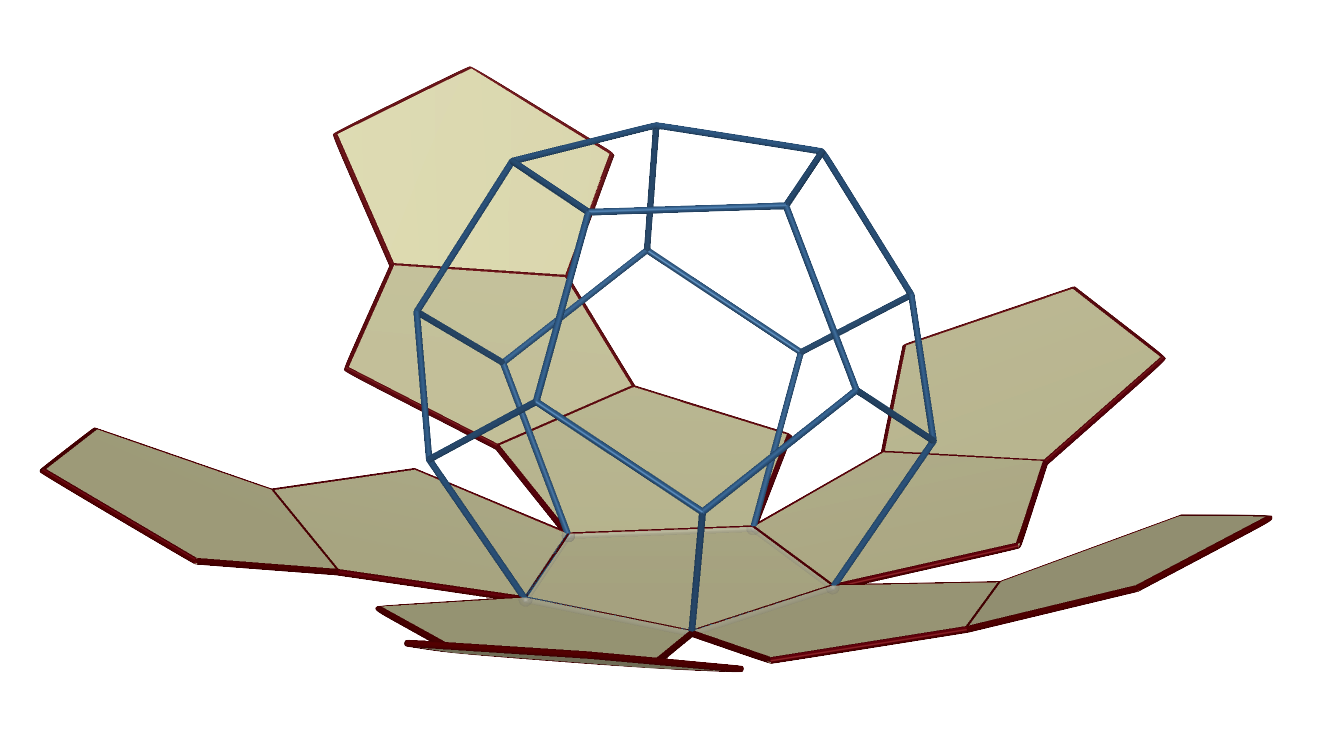
\includegraphics[width=0.9\textwidth]{img-00/portada}

\vspace{1.5cm}

 
\begin{minipage}{0.4\textwidth}
\begin{center}
	\includegraphics*[width=1.2in]{img-00/ies-binissalem-logo}
 
	\small
	
	\noindent \href{www.iesbinissalem.net}{\textbf{www.iesbinissalem.net}}  
 
\end{center}
\end{minipage}
\begin{minipage}{0.4\textwidth}
\begin{flushright}
\textbf{Josep Mulet}

\textit{Departament de Matemàtiques} 

 IES Binissalem
\end{flushright}
\end{minipage} 


\end{center}

\newpage

\vspace*{12.5cm}
 \begin{center}
 	\begin{minipage}{0.5\textwidth}
 		Aquesta és una obra derivada de ``\textit{Matematicas 3º de ESO. Ejercicios y problemas}'' de Marea Verde de matemàtiques. Per tant, està subjecta a les mateixes condicions de llicència CREATIVE COMMONS que l'obra original.
 		
 		 \noindent \textbf{Edició \LaTeX: \quad \textregistered \,  Josep Mulet Pol}
 		
 		 \noindent \textbf{Versió}: \quad 2017-07-23
 		 
 		 \noindent \textbf{Portada}: \quad \textit{Desenvolupament d'un dodecaedre}.
 		 
 		
 		\begin{center}
 		\includegraphics*[width=8cm]{img-00/licencia}
 		\end{center}
 	\end{minipage}
 \end{center}
 
%\clearemptydoublepage
%%\setcounter{page}{1}
%%\fancyfoot[C]{\roman{\thepage}}%

\renewcommand{\thepage}{\Roman{page}}% Roman numerals for page counter
\pagestyle{myheadings}
\thispagestyle{empty}
\renewcommand{\headrulewidth}{0pt}
\renewcommand{\footrulewidth}{0pt}

\pagebreak


\dominitoc

\tableofcontents

\newpage

\vspace*{\fill}
\begin{center}
	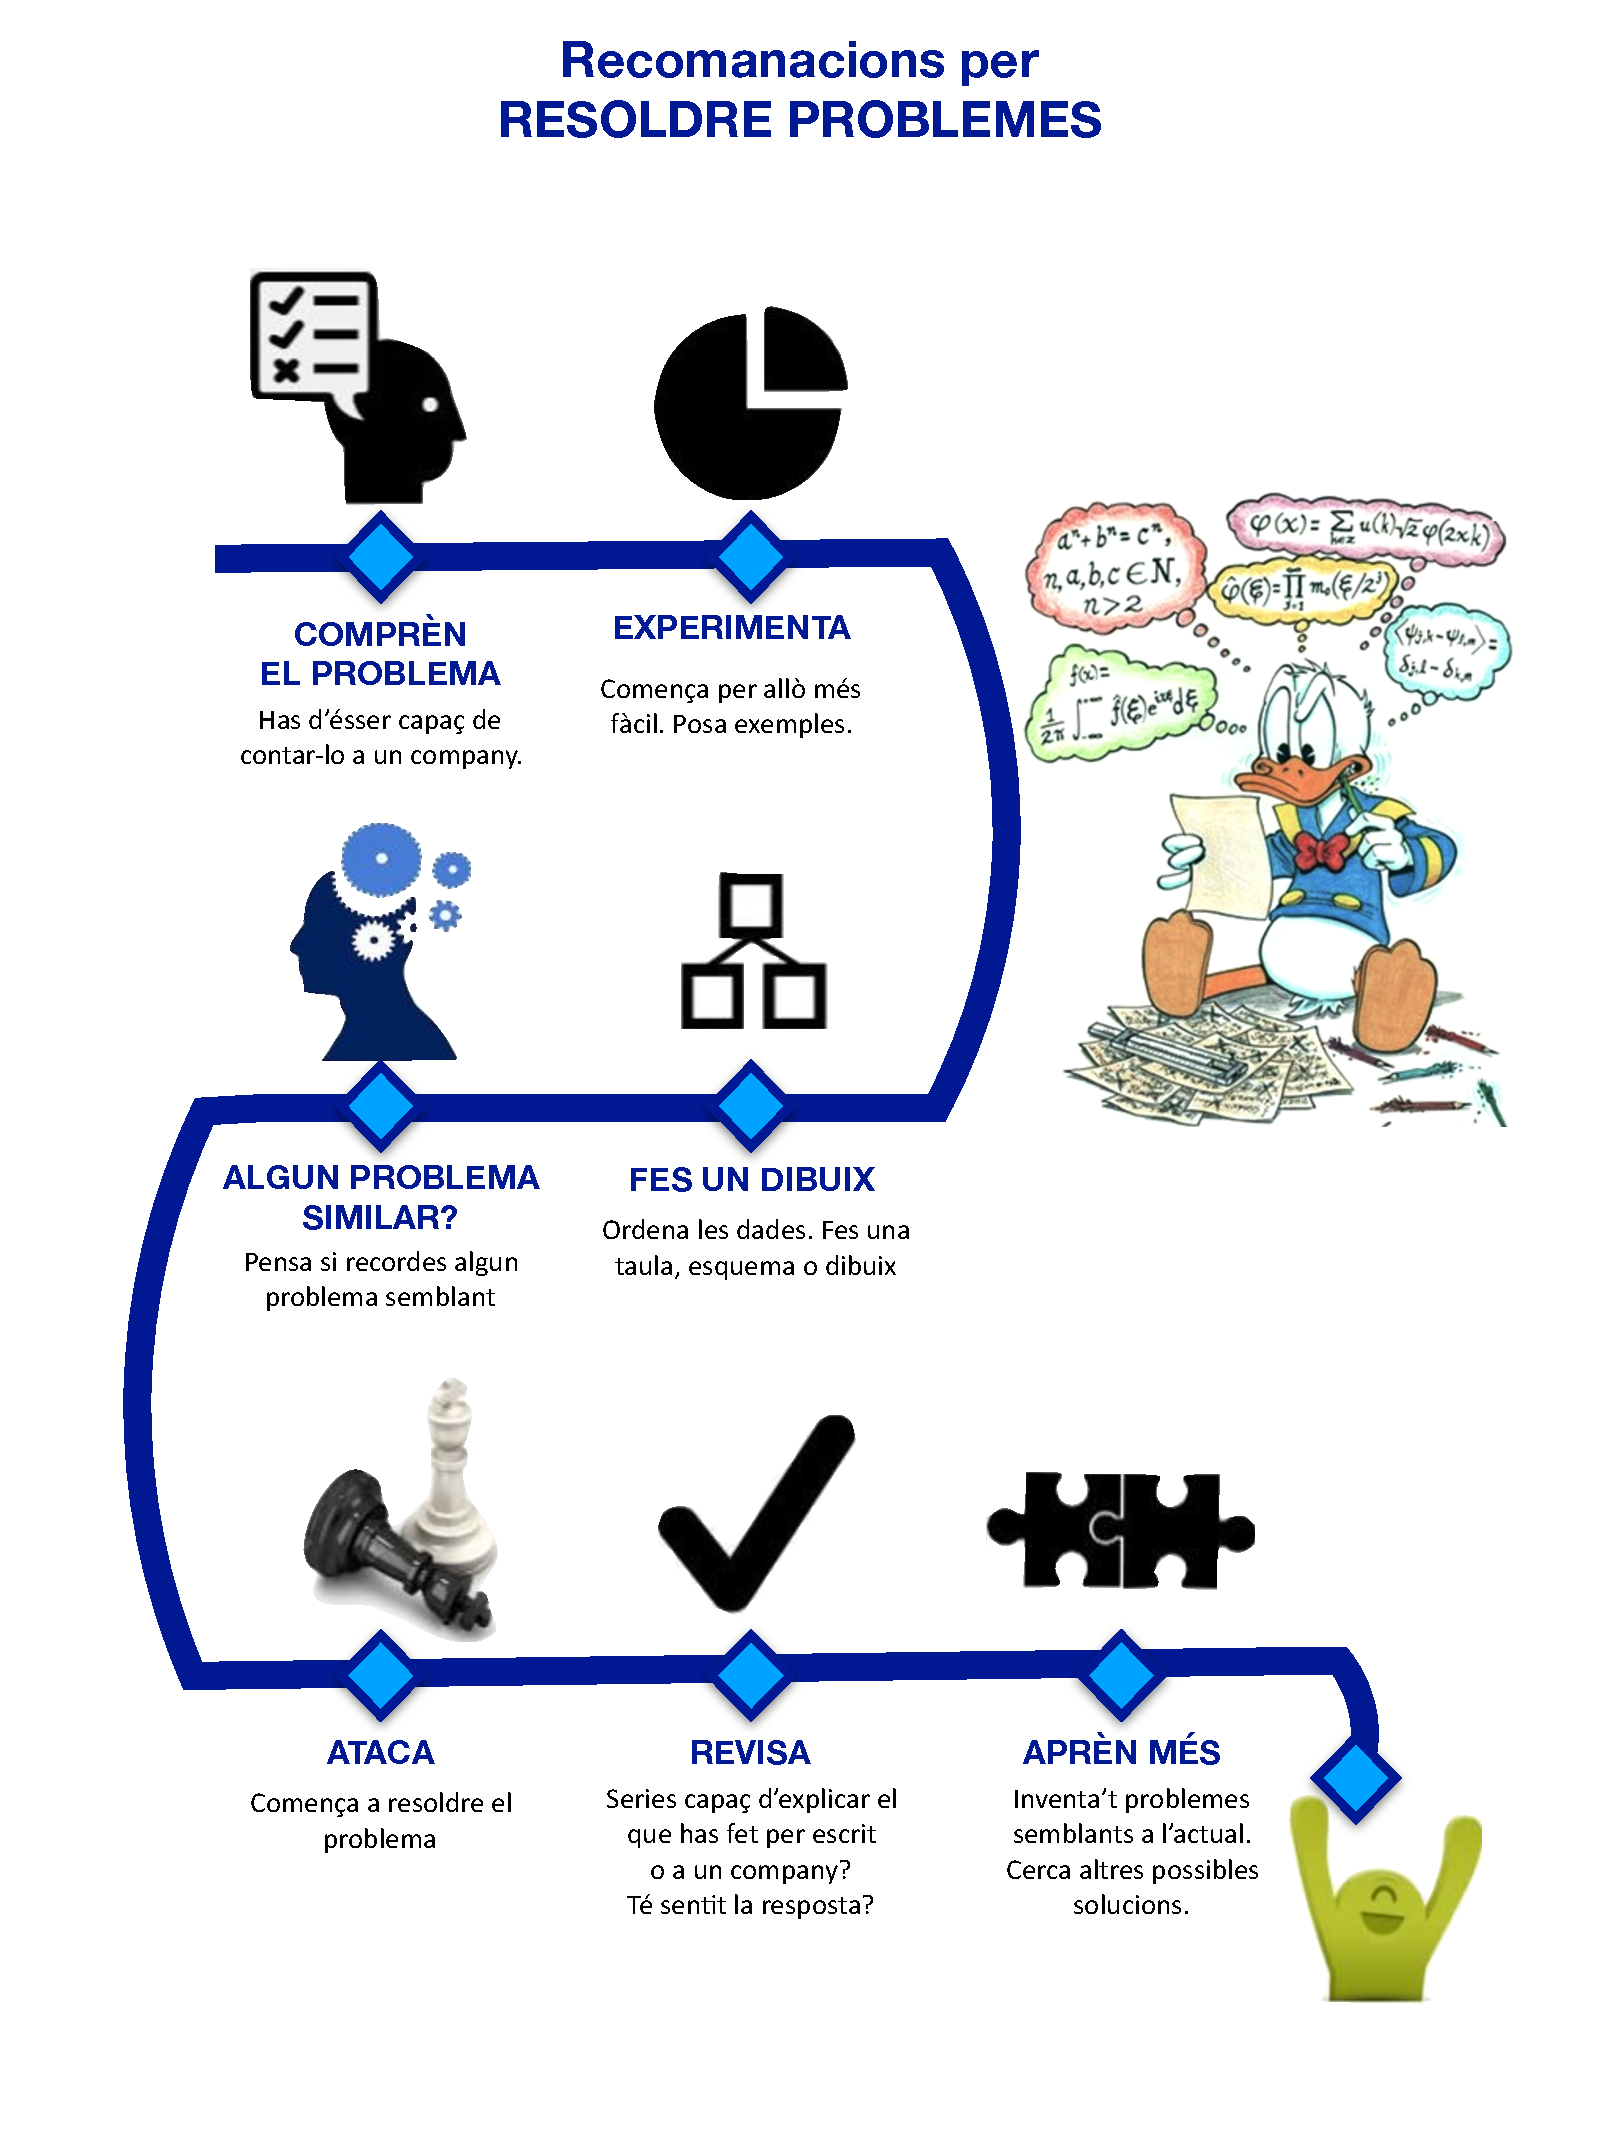
\includegraphics[width=\textwidth]{img-00/resolucio-problemes}
\end{center}
\vspace*{\fill}



\cleartorightpage


\vspace*{2cm} 
\heading{Símbols}

\begin{center}
	\renewcommand{\arraystretch}{1.5}
\begin{longtable}[h]{>{\raggedleft\arraybackslash}p{0.19\textwidth}|p{0.78\textwidth}}
	{\bfseries Símbol} & {\bfseries Significat} \\ \hline
	
	\simbolclau & Problema clau amb solució al final del llibre.  \\ \hline
	
	\simbolcompass & A més de la solució, proporciona orientacions per arribar a ella.  \\ \hline
	
	\simbolsearch & Problema que requereix d'investigació o recerca d'informació.  \\ \hline

	\ggb & Activitat adequada per realitzar amb el programa Geogebra.  \\ \hline
		
	\begin{center}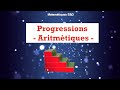
\includegraphics[width=1cm]{img-00/video-132}\par {\footnotesize Vídeo 132:}\end{center} & Explicació en vídeo dels continguts de l'apartat. El número de vídeo correspon a la numeració emprada en https://piworld.es 
	
	\\ \hline
	\hot[2] & Problema amb un cert grau de dificultat. \\ [0.25cm] \hline
	\spen & Activitat que es pot contestar en el llibre mateix. \\ [0.25cm] \hline 
	\mental & Activitat que es pot resoldre mentalment o en veu alta.
\end{longtable}
\end{center}
\vspace{1cm} 
 
\heading{Recursos}

\begin{center}
	\renewcommand{\arraystretch}{1.5}
\begin{longtable}[h]{>{\raggedleft\arraybackslash}p{0.2\textwidth}|p{0.8\textwidth}}
	\hline
	\textbf{piWorld}
	
	
\includegraphics[height=1.5cm]{img-00/piworld}
	 & Plataforma d'aprenentatge. Conté explicacions en vídeo i activitats interactives. Requereix usuari i contrasenya. \newline
	\href{https://piworld.es}{\href{https://piworld.es}{https://piworld.es}}
	\\ \hline
 	\textbf{Geogebra} 
 	
 	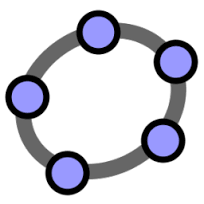
\includegraphics[height=1.5cm]{img-00/geogebra}
 	& Programa lliure de geometria dinàmica en dues i tres dimensions.
 	Ideal pels temes de funcions i geometria.\newline
 	\href{https://www.geogebra.org/download}{\href{https://www.geogebra.org/graphing}{https://www.geogebra.org/graphing}}
 	  \\ \hline
 	  	\textbf{Calculadora WIRIS}
 	 
 	  	
 	  	
\includegraphics[height=2cm]{img-00/wiris}
 	  	& Calculadora per al càlcul simbòlic. Nova versió Web \par \href{https://calcme.com/a}{https://calcme.com/a}
 	  	
 	  	La versió antiga la trobareu a \par \href{http://www.wiris.net/educa.madrid.org/wiris/es/cas.html}{http://www.wiris.net/educa.madrid.org/wiris/es/cas.html}
 	  	
 	  	 Atenció: requereix el plugin de Java i no funciona en dispositius mòbils.
 	  \\ \hline
 
 \end{longtable}
\end{center}
 


\mychapter{Nombres Racionals}
{Nombres Racionals}
{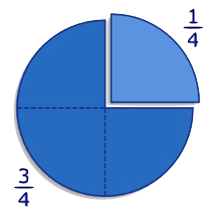
\includegraphics[width=4cm]{img-01/image1.png}}
{chap:racionals}
 
\vspace{1cm}
\begin{iniaval}
	\textbf{Completa:}
	
	\begin{itemize}
		\item En una fracció $\frac{a}{b}$, $a$ es diu ................................... i $b$ s'anomena \dotfill
		
		\item  Quan una fracció no es pot simplificar més es diu \dotfill
		
		\item  Quant val les dues terceres parts de 24?  \dotfill
		
		\item  Una botella de vi de 3/8 de litre; com s'expressa com a número decimal? \dotfill
	\end{itemize}
	
	\vspace{0.5cm}
	\textbf{Calcula i simplifica:}
	
	\begin{tasks}(2)
		\task $\frac{3}{4}+\frac{7}{2}-3=$    \task $\frac{3}{7}\cdot\frac{28}{6}=$
		
		\task $\frac{3}{4}:\frac{7}{2}=$      \task $\frac{3}{7} \text{ de } 42=$
	\end{tasks}	

	\vsoo
	\addanswersline{Avaluació inicial}{0}{$a$: numerador,\par $b$: denominador,\par irreductible,\par $\frac{2}{3} \text{ de } 24=16$,\par $\frac{3}{8}=0.375$ litres,\par
	\begin{tasks}(2)
			 \task $\frac{5}{4}$ \task $2$ \task $\frac{3}{14}$ \task $18$
	\end{tasks}	
	}
\end{iniaval}



\newpage
\section{Operacions amb nombres enters}

\begin{theorybox}[Prioritat de les operacions]
	\begin{tabular}{ll}
		& $3 - (-2)^{2} \cdot ( 4 - 9)$ \\
		\textbf{1r} Efectuam els parèntesi          &     $ 3 - (-2)^{2} \cdot (-5)$ \\
		
		\textbf{2n} Calculam potències i arrels        &    $ 3 - 4 \cdot (-5)$     \\
		
		\textbf{3r} Efectuam les multiplicacions i les divisions &  $ 3 + 20$ \\
		
		\textbf{4t }Finalment, feim les sumes i les restes.       &                      $23$
	\end{tabular}
\end{theorybox}

\begin{mylist}
	\exer  \spen  Calcula:

\begin{tasks}(2)
	\task  $-2 \cdot (-20 + 15)  =$    
	
	\task  $-20 : \left(10 - 2\cdot (-20 + 15) \right) =$      
	
	\task*(2) $\left[-80 -20 : \left(10 - 2\cdot (-20 + 15) \right) \right] \cdot (3 - 2 \cdot 3^{2})$=
	
\end{tasks}
\vso
 	\answers{[$10$, $-1$, $1215$]}



	\exer  \spen  Calcula pas a pas:   $(-5 + 4 \cdot (-2) +7) : (7 - (3 - 4)\cdot (-1))$
\vsoo
	\answers{$-1$}







	\exer  \spen  Calcula:

\begin{tasks}(2)
	\task $-10 + 20 : (-5) =$ 
 
	\task $-100 : \left[ (-20) : (-5) \right]=$ 
 
\end{tasks} 
\answers{[$-14$, $-25$]}



	
\exer[1]  Calcula:

\begin{tasks}(2)
\task $3-(4\cdot 3-2\cdot 5)^{2} -(3-5)^{3} $   \task $5-3^{2} -2\cdot (-5)-(7-9)^{2} $
\task $7-2\cdot (3-5)^{2} +2\cdot (-3)+8-(-2)^{2} $  \task $2-(2\cdot 3-3\cdot 4)^{2} -(2-4)^{3} $
\end{tasks} 
\answers[cols=2]{[$7$, $2$, $-3$, $-26$]}

\end{mylist}

\section{Operacions amb nombres racionals}

\begin{theorybox} 
\begin{multicols}{2}
	\centering
\videonw[ytid=ZzRAv1IAUig]{117}{Nombres racionals, operacions simples.}
\videonw[ytid=GX7auykiAA4]{118}{Nombres racionals, operacions combinades.}  
\end{multicols}
\end{theorybox}

\vspace{2cm}

\begin{mylist}
	
\exer[1] \spen Calcula i simplifica.
 
\begin{tasks}(2)
\task $\frac{3}{2} -\frac{3}{10} -\frac{3}{5} =$                \task  $\frac{7}{12} +\frac{4}{9} -\frac{1}{2} +\frac{3}{4} -\frac{7}{6} =$  

\vsoo

\task $\frac{1}{2} -\frac{3}{4} -\frac{2}{3} +1=$                \task $\frac{1}{11} -\frac{13}{22} -\frac{1}{4} +1=$

%\vsoo

%\task  1 -- $\frac{2}{3} +\frac{2}{5} -\frac{7}{5} =$               \task$\frac{4}{7} +\frac{1}{2} -\frac{8}{21} -\frac{5}{14} =$
\end{tasks}
\vsooo
\answers[cols=2]{[$\frac{3}{5}$, $\frac{1}{9}$, $\frac{1}{12}$, $\frac{1}{4}$]}

 
\exer[1] \spen  Calcula i simplifica.
 
 \begin{example}
 	 a) $\ \ \frac{7}{6} - \left(\frac{1}{2}-\frac{1}{3}\right)=\frac{7}{6}-\left(\frac{3}{6}-\frac{2}{6}\right)=\frac{7}{6}-\frac{1}{6}=\frac{6}{6}=1$
 	 \vspace{0.25cm}
 \end{example}

\begin{tasks}(2)
\task$\frac{7}{6} -\left(\frac{1}{2} -\frac{1}{3} \right)$=                   \task $2-\left(\frac{1}{2} -\frac{1}{3} \right)$=               
\vsoo

\task $\frac{6}{7} -\left(\frac{3}{7} -\frac{11}{14} \right)$=                    \task $\left(\frac{5}{6} +\frac{2}{5} \right)$$-\left(\frac{3}{5} +\frac{1}{6} \right)$=             
\vsoo

\task $\left(\frac{3}{4} +\frac{2}{5} +1\right)-\left(2-\frac{7}{5} \right)$=                 \task $\left(5-\frac{7}{2} \right)-\left(3+\frac{1}{4} \right)+\left(2-\frac{3}{8} \right)$ =
\vsoo

\task $\left(1+\frac{1}{2} +\frac{1}{4} \right)-$$\left(1+\frac{1}{3} +\frac{1}{6} \right)$=          \task $\left(\frac{11}{12} -\frac{3}{4} +\frac{1}{8} \right)-\left(\frac{1}{2} -\frac{2}{3} -\frac{5}{4} \right)$=
\end{tasks}
\vsooo
\answers[cols=2]{[$1$, $\frac{11}{6}$, $\frac{17}{14}$, $\frac{7}{15}$, $\frac{31}{20}$, $-\frac{1}{8}$, $\frac{1}{4}$, $\frac{41}{24}$]}


 
\exer[1]  Opera i simplifica.
 
\begin{tasks}(2)
\task $2\cdot \left(\frac{1}{2} -\frac{1}{6} \right)$=         \task $2:\left(\frac{1}{2} -\frac{1}{4} \right)$  =

\task $\left(\frac{2}{5} -\frac{1}{3} \right)\cdot 5$   =       \task $\frac{3}{7} :\left(1-\frac{1}{7} \right)$ =

\task  $\left(\frac{1}{2} +\frac{1}{4} \right)\cdot \left(1-\frac{1}{3} \right)$ =      \task$\left(1-\frac{1}{5} \right):\left(\frac{1}{2} +\frac{3}{10} \right)=$

\task $\left(5-\frac{1}{2} -\frac{7}{3} \right):\left(\frac{6}{5} -\frac{1}{3} \right)=$     \task $\left(1+\frac{1}{2} +\frac{1}{8} \right)\cdot \left(2-\frac{10}{13} \right)=$

\task $3\cdot \left(\frac{1}{2} +\frac{1}{3} \right)-2\cdot \left(2-\frac{1}{3} \right)=$                          \task $\frac{1}{2} \cdot \left(1+\frac{2}{5} \right)+2\cdot \left(1-\frac{3}{5} \right)=$

\task $\frac{2}{3} \cdot \left(\frac{1}{2} +\frac{2}{3} \right)-2\cdot \left(\frac{2}{3} -\frac{4}{9} \right)=$   \task $\frac{3}{4} \cdot \left[\frac{6}{5} -\frac{2}{7} \cdot \left(1+\frac{2}{5} \right)\right]$=
\end{tasks}
\answers{[$\frac{2}{3}$, $8$, $\frac{1}{3}$, $\frac{1}{2}$, $\frac{1}{2}$, $1$, $\frac{5}{2}$, $2$, $-\frac{5}{6}$, $\frac{3}{2}$, $\frac{1}{3}$, $\frac{3}{5}$]}
 
 \begin{comment}
	\exer  La mitjana harmònica es defineix com a $H(a,b)=\frac{1}{\frac{\frac{1}{a}+\frac{1}{b}}{2}}$, l'invers de la mitjana aritmètica dels inversos.
 

a) Demostra que H(a, b) = $\frac{2ab}{a+b} $  \quad\quad  b) Troba $H\left(\frac{3}{2} ,\frac{11}{3} \right)$ 
\end{comment}
 
	\exer \spen Troba la fracció inversa de $\mathrm{3+}\frac{\mathrm{4}}{\mathrm{5}}\mathrm{:}\frac{\mathrm{6}}{\mathrm{10}}=$
	\answers{$\frac{3}{13}$}
	
	\exer  \spen Opera i simplifica: $\frac{4}{5} \cdot \frac{6}{14} \cdot \frac{10}{12} \cdot \frac{7}{2}=$
	\answers{$1$}
	
	\exer  Resol pas a pas  $\frac{\frac{\mathrm{3}}{\mathrm{5}}\mathrm{-}\frac{\mathrm{2}}{\mathrm{5}}\mathrm{:}\frac{\mathrm{4}}{\mathrm{6}}}{\frac{\mathrm{3}}{\mathrm{5}}\mathrm{:}\left( \frac{\mathrm{1}}{\mathrm{6}}\mathrm{-}\mathrm{2}\right)}=$ 
	\answers{$0$}
	
	\exer \spen Simplifica:  
	\begin{tasks}(2)
	\task $\; \frac{2\cdot 7\cdot 15}{21\cdot 10} = \quad \quad \quad$
	
	%%\task $\; \frac{10+6}{10-2} \quad \quad \quad$ 
	
	\task $\; \frac{2\cdot 3+4}{2\cdot 5+10}= $
	\end{tasks}
	\answers[cols=2]{[$1$, $\frac{1}{2}$]}

	\exer[1]  Calcula: 
 \begin{tasks}(3)
 	\task $\frac{2}{3} \cdot \left(\frac{3}{2} :\frac{1}{3} \right)^{2} +\left(2-\frac{1}{2} \right)^{2} $ 
 	\task $\frac{3}{4} \cdot \left(\frac{3}{2} :\frac{3}{4} \right)^{3} +\left(2-\frac{3}{2} \right)^{2} $ 
 	\task $\frac{8}{3} \cdot \left(\frac{3}{4} :\frac{1}{2} \right)^{2} +\left(\frac{1}{2} -1\right)^{3} $ 
 \end{tasks}
 \answers[cols=2]{[$\frac{67}{4}$, $\frac{25}{4}$, $\frac{47}{8}$]}


\end{mylist}

\newpage
\section{Representació de fraccions sobre la recta numèrica}
 
\begin{theorybox}
\video[rows=4,ytid=FXWcB8irMk8]{153}{Representació de fraccions \vspace{-0.5cm}}

\textbf{Classificam les fraccions en tres tipus:}

- Fraccions \textbf{pròpies} (menors que la unitat): $\frac{1}{2},\frac{2}{3},\frac{5}{9},$ ···

- Fraccions \textbf{iguals a la unitat}: $\frac{2}{2},\frac{3}{3},\frac{4}{4},$ ···

- Fraccions \textbf{impròpies} (majors que la unitat): $\frac{7}{2}, \frac{11}{3}, \frac{-49}{5}, \cdots$·

Les fraccions impròpies es poden expressar com un\textbf{ número mixt}:  
$\frac{7}{3}=\ 2\ +\frac{1}{3}$

\end{theorybox}


\begin{mylist}
	\exer \spen  Passa a forma mixta les següents fraccions: $\frac{50}{7} ;\frac{25}{11} ;\frac{101}{6} $
 \vsooo
	\answers[cols=2]{[$7+\frac{1}{7}$, $2+\frac{3}{11}$, $16+\dfrac{5}{6}$]}
 
	\exer \spen Passa a forma mixta les fraccions $\frac{-30}{7} ;\frac{-50}{13} ;\frac{-100}{21} $ 
 \vsooo
	\answers[cols=2]{[$-4-\dfrac{2}{7}$, $-3-\dfrac{11}{13}$, $-4-\dfrac{16}{21}$]}
 
	\exer \spen Representa en la recta numèrica les fraccions: $\frac{1}{5} ;\frac{3}{7} ;\frac{-5}{8} ;\frac{-3}{4} $ 
	\begin{center}
	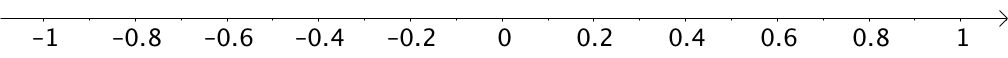
\includegraphics[width=0.9\textwidth]{img-01/rectanum11}
	\end{center}
	\answers{Gràfica:\par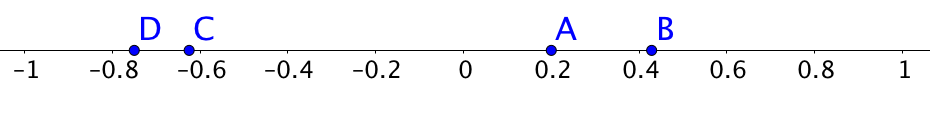
\includegraphics[width=0.45\textwidth]{img-sol/t1-recta1}}
 \vsooo
 
	\exer \spen Passa a forma mixta i representa les fraccions: $\frac{23}{8} ;\frac{-23}{8} ;\frac{180}{50} ;\frac{-26}{6} $ 
	\begin{center}
		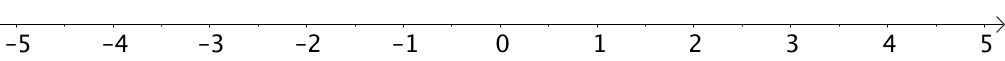
\includegraphics[width=0.9\textwidth]{img-01/rectanum}
	\end{center}
	\answers{Gràfica:\par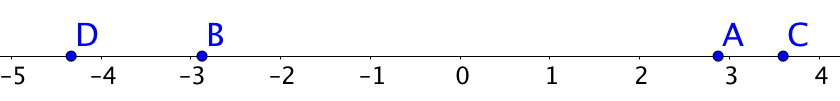
\includegraphics[width=0.45\textwidth]{img-sol/t1-recta2}}
 \vsooo
\newpage
 
	\exer \spen  Troba les fraccions que es corresponen amb els punts \textit{A, B, C, D} i \textit{E, }expressant\textit{ }en forma mixta i com a fracció impròpia les representades pels punts \textit{A, B} i \textit{E}.
 
\includegraphics*[width=0.93\textwidth]{img-01/image4.png}

A=\quad\quad\quad\quad\quad\quad B=\quad\quad\quad\quad\quad\quad  C=\quad\quad\quad\quad\quad\quad  D=\quad\quad\quad\quad\quad\quad E=\quad\quad\quad\quad\quad\quad
 \vsooo
 \answers{$A=-2-\dfrac{2}{9}=-\dfrac{20}{9}$;\par $B=-1-\dfrac{6}{8}=-\dfrac{14}{6}$;\par $C=-\dfrac{3}{4}$;\par $D=\dfrac{3}{5}$;\par $E=2+\dfrac{4}{7}=\dfrac{18}{7}$}

\end{mylist}

\section{Fraccions i decimals}
 
\begin{theorybox}
\video[ytid=12GEHAqGpzA]{119}{Nombres racionals: Relació entre fracció i decimal.}

Els nombres decimals es classifiquen en: 

- \textbf{Exactes}:  com $1,25=\ \frac{125}{100}$

- \textbf{Periòdics}:   Són Fraccions
	
	\quad\quad\quad \textbf{Pur}$\boldsymbol{:}\ 3,626262\textrm{·}\textrm{·}\textrm{·}=3,\widehat{62}$ $=\ \frac{362-3}{99}=\frac{359}{99}$               

	\quad\quad\quad \textbf{Mixt: }$7,19999\textrm{·}\textrm{·}\textrm{·}\textrm{·}=7,1\hat{9}=\frac{719-71}{90}=\frac{648}{90}$

\textbf{- No periòdics}: com el número $\pi$, $\sqrt{2}, \cdots$. No són fraccions.
\end{theorybox}




\begin{mylist}
	\exer  Sense fer la divisió indica si les següents fraccions tenen expressió decimal exacta o periòdica:
 
\begin{tasks}(4)
	\task  $\frac{21}{750} $ 
	\task $\frac{75}{21} $
	\task $\frac{11}{99} $
	\task $\frac{35}{56} $
\end{tasks} 
	\answers[cols=2]{[Exacte, Periòdic, Periòdic, Exacte]}

\textit{Ajuda}: \textit{La divisió és exacta només quan la descomposició del denominador conté únicament 2 o 5.}

 
	\exer Passa a fracció i simplifica:
	\begin{tasks}(3)
		\task 1,4142  
		\task 0,125 
		\task 6,66
	\end{tasks}
 	\answers{[$\dfrac{7071}{5000}$, $\dfrac{1}{8}$, $\dfrac{333}{50}$]}
	
	\exer Passa a fracció i simplifica:
 \begin{tasks}(3)
 	\task 1,41424142{\dots}  
 	\task 0,125125{\dots} 
 	\task 6,666{\dots}
 \end{tasks}
	\answers{[$\dfrac{14141}{9999}$, $\dfrac{125}{999}$, $\dfrac{20}{3}$]}
 
 
	\exer  Passa a fracció i simplifica:
 \begin{tasks}(3)
 	\task 1,04444{\dots} 
 	\task  0,7125125{\dots}
 	\task  6,7666{\dots}
 \end{tasks}
	\answers{[$\dfrac{47}{45}$, $\dfrac{3559}{4995}$, $\dfrac{203}{50}$]}

\vspace{2cm}
 
	\exer  \spen  Completa la taula següent
 
\begin{tabular}{|p{0.28\textwidth}|p{0.28\textwidth}|p{0.28\textwidth}|} \hline 
	\rowcolor{lightgray} Decimal & Fracció & Percentatge \% \\ \hline 
	0,75 &  &  \\ \hline 
	& 6/4 &  \\ \hline 
	&  & 68\% \\ \hline 
\end{tabular}
\answers{
	{\renewcommand{\arraystretch}{1.8}
	\begin{tabular}{|c|c|c|} \hline 
		\rowcolor{lightgray} Decimal & Fracció &  \% \\ \hline 
		0,75 &  $\frac{3}{4}$ & 75 \%  \\ \hline 
		1,5 & $\frac{6}{4}$ & 150 \% \\ \hline 
		0,58 & $\frac{17}{25}$ & 68\% \\ \hline 
	\end{tabular}}
}

 
	\exer  Calcula el número decimal que correspon al percentatge 130\% i el percentatge que correspon a la fracció 7/25.
 \answers{$130$ \%=$0.13$ i $\frac{7}{25}=28$ \%}


 
\exer[1]  Calcula, passant prèviament a fracció cada nombre decimal: 
 \begin{tasks}(3)
 	\task 0,333{\dots} + 0,666{\dots} 
 	\task 0,888{\dots} $\cdot$ 2,5
 	\task 0,65 : 0,656565{\dots}
 \end{tasks}
\answers[cols=3]{[$1$, $\dfrac{20}{9}$, $\dfrac{99}{100}$]}

\end{mylist}

\begin{example}
 
$\mathrm{1,66666\textrm{·}\textrm{·}\textrm{·}\ -\ 1,0222\textrm{·}\textrm{·}\textrm{·}\ =1,}\widehat{\mathrm{6}}\mathrm{-}\mathrm{1,0}\widehat{\mathrm{2}}\mathrm{=}\frac{\mathrm{16-1}}{\mathrm{9}}\mathrm{-}\frac{\mathrm{112-10}}{\mathrm{90}}\mathrm{=}\frac{\mathrm{15}}{\mathrm{9}}\mathrm{-}\frac{\mathrm{102}}{\mathrm{90}}\mathrm{=}\frac{\mathrm{48}}{\mathrm{90}}\mathrm{=}\frac{\mathrm{8}}{\mathrm{15}}$
\vspace{0.25cm}
\end{example}


\begin{mylist} 
 
	\exer  Demostra que 4,999{\dots} = 5. Generalitza: Quant val n,999{\dots}?
 
 	\answers{$4,999{\cdots}=4,\hat{9}=\frac{49-4}{9}=\frac{45}{9}=5$.\par En general:
 	$n,999{\cdots}=n,\hat{9}=\frac{10n+9-n}{9}=\frac{9n+9}{9}=n+1$
 }


 
	\exer  Representa de forma exacta en la recta numèrica: $\frac{760}{240};\ \ 3,125;\ -\frac{46}{14}$; -2,1666{\dots}
	
	\answers{Gràfica:\par 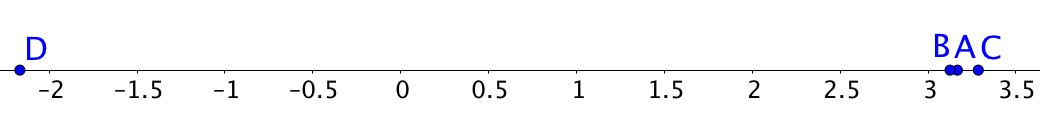
\includegraphics[width=0.5\textwidth]{img-sol/t1-recta3}}
\end{mylist}

\section{Ordenar fraccions}
 

\begin{theorybox}
\video[ytid=I6Arx0Z6o2M]{152}{Nombres racionals.}  

\textbf{Per ordenar fraccions ho podem fer de dues formes diferents:}

- Reduir les fraccions a denominador comú (mín. c. m.)

- Convertir les fraccions a nombre decimal i ordenar els números decimals
\vspace{0.25cm}
\end{theorybox}

\begin{mylist}
	 

 
	\exer  Ordena de menor a major: $\frac{7}{12},\frac{4}{6},\frac{5}{9},\frac{3}{4},\frac{13}{18}$

\end{mylist}	

	\begin{example}[*]
		\textbf{Primer mètode}: Reduir a denominador comú.
				$min.c.m(12, 6, 9, 4, 18) = 36$
		
		$\frac{7}{12},\frac{4}{6},\frac{5}{9},\frac{3}{4},\frac{13}{18}$  \quad $\rightarrow$ \quad $\frac{21}{36},\frac{24}{36},\frac{20}{36},\frac{27}{36},\frac{26}{36}$
		
		Ordenam de menor a major les fraccions originals $\frac{5}{9} < \frac{7}{12} < \frac{4}{6} < \frac{13}{18} < \frac{3}{4}$
		
		\textbf{Segon mètode}: Valor decimal
		
		$\frac{7}{12},\frac{4}{6},\frac{5}{9},\frac{3}{4},\frac{13}{18}$  \quad $\rightarrow$ \quad $0.8\hat{3}, 0.\hat{6}, 0.\hat{5}, 0.75, 0.7\hat{2}$
		
		i ordenam els nombres decimals de menor a major i trobam el mateix resultat que abans.
		
	\end{example}
 


\begin{mylist}


	\exer  Ordena de menor a major: $\frac{8}{9} ;\frac{-8}{9} ;\frac{4}{5} ;\frac{38}{45} ;\frac{77}{90} ;\frac{-9}{8} $
	\answers{$\frac{-9}{8}< \frac{-8}{9}<\frac{4}{5} <\frac{38}{45} <\frac{77}{90}  < \frac{8}{9}$}


 
	\exer  Ordena de menor a major: $\frac{11}{24},\ -\frac{7}{4},\frac{3}{8},\ -\frac{1}{6},\frac{5}{12},\ -\frac{5}{3}$
 \answers{$-\frac{7}{4}<-\frac{5}{3}<-\frac{1}{6}<\frac{3}{8}<\frac{5}{12}<\frac{11}{24}$}
 



 
	\exer  Suposa que tens dues fracció $a$ i $b$ i vols trobar el nombre que es troba just enmig. Explica com ho faràs. Inventat un exemple i representa les tres fraccions sobre la recta numèrica.
	
	\redacta
	\answers{El que començam fent és sumar les dues fraccions $a$ i $b$. Després el resultat en dividim entre dos. D'aquesta forma tenim el nombre que està enmig. Per exemple: si $a=\frac{2}{3}$ i $b=\frac{5}{4}$,
	\[\frac{2}{3} +\frac{5}{4} =\frac{8}{12} + \frac{}{12} = \frac{23}{12} \]	
	Finalment dividim entre dos: La fracció és $ \frac{23}{24} \approx 0,958\hat{3}$
	\par
	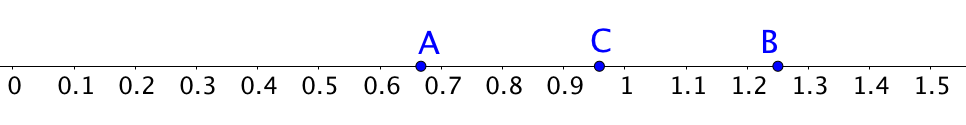
\includegraphics[width=0.5\textwidth]{img-sol/t1-recta4}
}
\end{mylist}
 
\section{Problemes de fraccions}
\begin{theorybox} 
\begin{minipage}{0.5\textwidth}
	\centering
	\videonw[ytid=o9DhLJxyPz0]{120}{Nombres racionals: Problemes tipus Part-Fracció-Total}
\end{minipage}
\begin{minipage}{0.5\textwidth}
	\centering
	\videonw[ytid=O9HQD38HBL8]{154}{Nombres racionals: Problemes típics amb fraccions}
\end{minipage}


\textbf{- Recorda l'essencial:}
\[\text{Fracció} = \frac{Part}{Total} \quad\quad\quad Part=\text{Fracció} \cdot Total   \quad\quad\quad  Total = \frac{Part}{\text{Fracció}}\]
\textbf{- Totes les fraccions de les parts sumen 1}

\end{theorybox}

\begin{mylist}
	\exer \spen  Calcula les dues terceres part de la sisena part del 80\% de 900.
 \vso
 \answers{80}

 
	\exer  \spen  Troba el nombre tal que els seus quatre terços valen 520.
 \vsoo
\answers{390}



 
	\exer  \spen  Quants pots de tres vuitens de litre puc omplir amb 12 litres?
 \vso
\answers{32 pots}
 
	\exer  Inventat un problema on aparegui la fracció $\frac{2}{5}$ i el nombre $200$. Resol aquest problema i comparteix-lo amb el teus companys. 
	 
	 \answers{Per exemple: En el nostre institut les $\frac{2}{5}$ parts dels alumnes de 3r d'ESO són d'Alaró. Si en total hi ha $200$ alumnes a 3r d'ESO, quants són d'Alaró?\par
	 \par Solució: $\frac{2}{5}$  de $200$ = 80 alumnes són d'Alaró.}  
\redacta

\pagebreak
\mbox{}
\vspace{-1cm} 
 
 \exer \begin{minipage}[t]{0.56\textwidth}  Si 100 polzades són 254 cm:
 
\begin{tasks}
	\task Troba el llarg en centímetres d'una televisió si l'altura són 19,2 polzades i llarg/alt = 4/3
	\task Igual però ara llarg/alt = 16/9
\end{tasks}
\answers{[65.024 cm, 86.6986 cm]} 

\end{minipage}
\begin{minipage}{0.44\textwidth}
	\centering
	\vspace{0.5cm}
	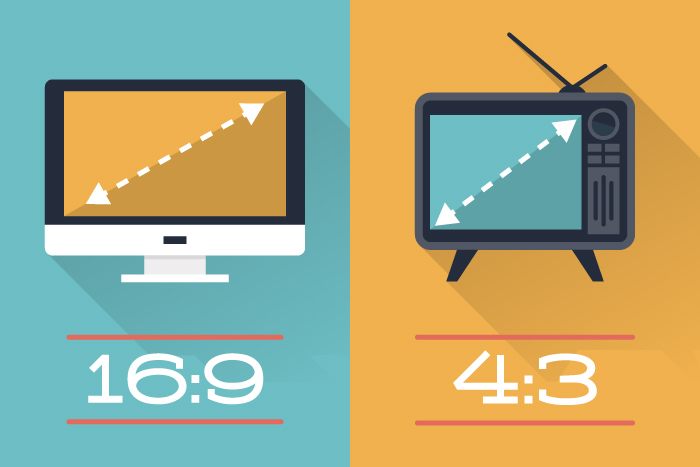
\includegraphics[width=0.7\textwidth]{img-01/tvs}
\end{minipage}

 
	\exer  Si en una classe el 77,777{\dots} \% dels alumnes aproven i hi ha més de 30 alumnes però menys de 40, quants alumnes són i quants aproven? \textit{Ajuda: Passa $77,\hat{7}$ a fracció.}
 
\answers{$77,7...= \dfrac{700}{9}$; Són 36 alumnes en total dels quals aproven 28}


\vspace{-0.75cm}
	\exer  
	\begin{minipage}[t]{0.8\textwidth}
	Després dels resultats de la jornada de futbol d'aquest cap de setmana, el Osasuna ha jugat 24 partits, dels quals ha guanyat 6 i ha empatat els 5/12. Quants partits ha perdut? Quin percentatge representen els 6 partits guanyats sobre el total de partits jugats?
	\end{minipage}
	\begin{minipage}{0.2\textwidth}
		\centering
		\vspace{0.5cm}
		
\includegraphics[width=1.5cm]{img-01/balon}
	\end{minipage}
\answers{Perden 8 partits (10 empatats). $\dfrac{6}{24}=25$ \%}


	\exer  Una fundació té un dipòsit de diners per premiar joves artistes. D'aquests diners, la meitat seran per al primer premi, la tercera part per al segon premi, la dotzena part per al tercer premi i els 2.000 € que, d'aquesta manera, sobren es reservaran per a properes edicions. Quants diners rebrà cada premiat ?
\answers{Total 24000 \euro{}; 1r: 12000 \euro{}, 2n: 8000 \euro{}, 3r: 2000 \euro{} }




	\exer  En una escola hi ha 1800 alumnes, dels quals 860 són noies. Els 3/4 de les noies i els 2/5 dels nois practiquen natació. Quants alumnes en total practiquen natació?

\answers{645 nines + 376 nins = 1021 alumnes practiquen natació.}



	\exer  Una empresa disposa de 7.200 € de pressupost mensual, del qual tres cinquenes parts es dediquen a pagar els sous dels treballadors, una quarta part a cobrir despeses comunes, i amb la resta es fa un fons d'estalvi per possibles imprevistos.


a ) Quina fracció del pressupost es destina a aquest fons d'estalvi? Quin percentatge del sou mensual representa?

b ) Quants diners s'han estalviat a l'acabar l'any ?

\answers{[$\dfrac{3}{20}=15$ \%, $12960$ \euro{}]}


	\exer  Una mare divideix el contingut d'una caixa de llepolies entre els seus tres fills; al primer li dóna la meitat del total, al segon, dues cinquenes parts del total, i al tercer, les 6 que queden. 


a) Quantes llepolies conté la caixa? 

b ) Quantes llepolies toquen a cada un dels fills?
\vspace{0.5cm}

\answers{La caixa conté 60 llepolies. Primer fill 30, segon fill 24 llepolies.}

\end{mylist}

\begin{example}[*]
	Entre els dos primers fills tindran $\frac{1}{2} + \frac{2}{5}= \frac{9}{10}$.
	%%
	Per tant, el tercer fill tindrà $1-\frac{9}{10}= \frac{1}{10}$.
	
	Sabem que aquesta fracció del total $x$ correspon a 6 llepolies.
	$\frac{1}{10} \text{ de } x = 6$ \quad $\rightarrow$ \quad $x=60$.
	
	Ara ja sabem que la caixa conté 60 llepolies. Sabries calcular quantes li toquen al primer i segon fill?
	
\end{example}

\pagebreak


\begin{mylist}
	
	\exer  Marta té 1.500 € al seu compte corrent. Gasta 1/3 en una cadena musical i 2/5 en una reparació del cotxe. Quants diners li queden?
\answers{100 \euro{}}




	\exer  A la selecció per a un concurs televisiu, passen la primera prova 5/12 dels aspirants i en la segona prova passen 4/13 dels que quedaven.


a ) Expressa en forma de fracció els aspirants que han estat seleccionats pel concurs.

b) Si 130 aspirants van passar la primera prova, quants aspirants es van presentar inicialment?
\answers{[7/39, Es van presentar 312 aspirants]}



	\exer   Per a la construcció d'un poliesportiu, l'Ajuntament aporta 1/10 del cost, la Unió Europea, 1/6 parts, el Govern, 4/15 parts, i la resta s'aconsegueix amb un préstec.


a ) Calcula la fracció del cost que representa el préstec.

b ) Si el Govern aporta 416.000 euros, calcula el cost total d'aquesta obra.

\answers{[7/15, 1.560.000 \euro{}]}


	\exer  Un alumne ha de llegir una novel·la en quatre setmanes. La primera setmana llegeix 5/12 de la novel·la, la segona setmana llegeix 5/24 i la tercera setmana llegeix 2/8 de la novel·la.


a ) Quina fracció de la novel·la ha de llegir la quarta setmana ?

b ) Si la novel·la té 216 pàgines, quantes ha llegit cada setmana ?
\answers{[1/8, 90; 45; 54; 27 cada setmana]}


	\exer  
	\begin{minipage}[t]{0.7\textwidth}	
	  Quantes botelles de 3/4 de litre necessit per tenir la mateixa quantitat que en 60 botelles de 3/5 de litre?
\end{minipage}
\begin{minipage}[t]{0.3\textwidth}
	\centering
	\vspace{-1.75cm}
	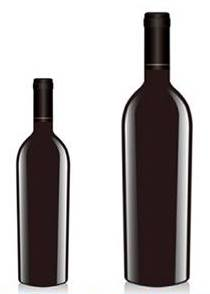
\includegraphics[width=0.4\textwidth,valign=t]{img-01/botellas}
\end{minipage}
\answers{48 botelles}


	\exer  Troba un nombre enter de tal forma que: la seva meitat, la seva tercera part, la seva quarta part, la seva cinquena part, la seva sisena part i la seva setena part siguin nombres enters.
\answers{$2\times 3\times 4\times 5\times 6\times 7=5040$ o també 420.}






	\exer  A la unitat li llevo les seves dues cinquenes parts. Per quina fracció cal multiplicar el resultat per arribar una altra vegada a la unitat?
\answers{Cal multiplicar per la fracció $\dfrac{5}{3}$}




	\exer  Troba la fracció resultant:


a) Llevo 1 terç del que tinc i després afegeixo 1 terç del que queda.

b) Afegeixo 1 terç del que tinc i després llevo 1 terç del resultat.

\answers{[$\dfrac{8}{9}$, $\dfrac{8}{9}$]}




	\exer  Estàs avorrit i decideixes jugar al següent: Avances un metre en línia recta, retrocedeixes la meitat, avances la meitat del que has retrocedit en l'últim pas, retrocedeixes la meitat del que has avançat en l'últim pas, {\dots}


Si ho fas moltes, però que moltes vegades, quant avances en total?
\[1-\frac{1}{2} +\frac{1}{4} -\frac{1}{8} +\frac{1}{16} -\frac{1}{32} +...=\] 
\answers{2/3 de metre.}



\begin{comment}
	\exer  \includegraphics*[bb=0 0 1.24in 1.25in, width=1.24in, height=1.25in, keepaspectratio=false]{img-01/image8.png} La figura del costat és un ``Tangram''.


a) Troba la fracció que es correspon amb cadascuna de les 7 peces.

b) Si el costat del quadrat és de 20 cm, troba l'àrea de cada peça.
\end{comment}

\end{mylist}


\pagebreak

\section{Aproximacions i errors}
 
\begin{theorybox}
Si d'una quantitat sabem el valor exacte i el valor aproximat, definim

L'error absolut és E${}_{A}$ = {\textbar}Valor exacte -- Valor aproximat{\textbar}

L'error relatiu és E${}_{R}$ = E${}_{A}$ / Valor exacte

Per exemple, si aproximem el número $\pi$ per 3,14 els errors comesos són:

E${}_{A}$ = {\textbar}$\pi$ -- 3,14{\textbar} =0,0016

E${}_{R}$ = 0,0016 / $\pi$ = 0,0005    =    0,05 \%

\end{theorybox}

\begin{mylist}
	\exer  \spen  Copia aquesta taula en el teu quadern i arrodoneix amb el nombre de xifres indicat


\begin{tabular}{|p{0.15\textwidth}|p{0.15\textwidth}|p{0.15\textwidth}|p{0.15\textwidth}|p{0.15\textwidth}|} \hline 
	\rowcolor{lightgray} \textbf{} & \multicolumn{4}{|p{2.5in}|}{\textbf{Xifres significatives}} \\ \hline 
	\textbf{Nombre} & 1 & 2 & 3 & 4 \\ \hline 
	\textbf{$\sqrt{10} $} &  &  &  &  \\ \hline 
	\textbf{1/7} &  &  &  &  \\ \hline 
	\textbf{95549} & 100000 &  &  &  \\ \hline 
	\textbf{30000} & 3·10${}^{4}$ &  &  &  \\ \hline 
	\textbf{1,9995} &  &  &  & 2,000 \\ \hline 
\end{tabular}
\answers{\begin{tabular}{|p{0.15\textwidth}|p{0.15\textwidth}|p{0.15\textwidth}|p{0.15\textwidth}|p{0.15\textwidth}|} \hline 
		\textbf{} & \multicolumn{4}{|p{0.6\textwidth}|}{Xifres significatives} \\ \hline 
		\textbf{Nombre} & 1 & 2 & 3 & 4 \\ \hline 
		\textbf{$\sqrt{10} $} & 3  & 3.2 & 3.16 & 3.162 \\ \hline 
		\textbf{1/7} & 0.1 & 0.14 & 0.143  & 0.1429 \\ \hline 
		\textbf{95549} & 100000 & 96000 & 95500 &  95550\\ \hline 
		\textbf{30000} & 3·10${}^{4}$ & 30·10${}^{3}$ & 300·10${}^{2}$ & 3000·10${}^{1}$  \\ \hline 
		\textbf{1,9995} & 2 & 2,0 & 2,00 & 2,000 \\ \hline 
\end{tabular}}


	\exer  Prova que 123,45 amb $E_A = 0,005$ i 0,12345 amb $E_A = 0,000005$ tenen el mateix $E_R$.
	\answers{Els dos tenen com $E_R=4.05\cdot 10^{-3}$}
	
	\exer  Contesta Vertader o Fals i justifica la teva resposta:


a) Per a una mateixa màquina, l'error comès és menor com més petita sigui la mesura.

b) No es poden comparar errors relatius de diferents magnituds.

c) Posar preus com 1,99 €/Kg és un intent d'engany.

d) Comprar a 1,99 €/Kg enfront de 2 €/Kg suposa un estalvi.

e) Posar moltes xifres en un resultat significa que un és un gran matemàtic.

f) La precisió es mesura pel nombre de xifres decimals.

\answers[cols=2]{[Depèn si $E_R$ o $E_A$, F, V, F, F, V]}


	\exer  Aproxima els nombres 32567 i 1,395 amb 2 xifres significatives i digues en quin es comet menor error relatiu.
	\answers{$32567=33000$ amb $E_R=0.013$ i $1,395=1,400$ amb $E_R=0.0036$}
	
	\exer  $\pi$ no pot representar-se mitjançant una fracció d'enters però, pots trobar una fracció que ho aproximi amb 5 xifres significatives? 
	\answers{$3.1416 = \dfrac{31416}{10000}=\dfrac{3927}{1250}$}
	
	\exer  Aproximem $\pi$ per $3+\frac{1}{7+\frac{1}{16} } $:
	

a) Simplifica fins a una fracció impròpia irreductible.

b) Troba l'error absolut i l'error relatiu.

\answers{[$\dfrac{355}{113}$, $E_A=2.67\cdot 10^{-7}$, $E_R=8.5\cdot 10^{-6}$]}

\end{mylist}


\newpage
\begin{autoaval}{51}

\begin{mylist}
	\exer[2]  Resol pas a pas: $(-8 - 7 \cdot (-4 + 6) : (2 + (-3)) + 5 - 4 · 2^{2}) \cdot (-2)$
	\answers{10}


	\exer[2] Ordena de major a menor:
	$\frac{5}{6} \, ;\frac{7}{8} ;\, \frac{-7}{8} ;\frac{-5}{6} ;\, \frac{-5}{4}$
	\answers{$\frac{7}{8}>\frac{5}{6}>\frac{-5}{6}>\frac{-7}{8}>\frac{-5}{4}$}
	
	\exer Representa sobre la recta numèrica:
	$\frac{3}{4} ;\, \frac{17}{6} ;\, \frac{-11}{7} ;\, -0,125$
	
	\exer[2]  Resol pas a pas i simplifica:
	$\frac{\frac{2}{3} -\frac{5}{6} :\left(2-\frac{11}{3} \right)}{\frac{2}{6} } $
	\answers{$\frac{7}{2}$}
	
	\exer[2]  
a) Troba les quatre cinquenes parts dels cinc vuitens de 360.

b) Una ampolla té plenes les seves set vuitenes parts, si conté 840 cm${}^{3}$, quant li cap plena?
	\answers{[180, 960 cm${}^3$]}

	\exer[2]  Aproxima els nombres 9859 i 9,945 amb 2 xifres significatives i calcula els errors relatius comesos (en \%), quin és menor?
	\answers[cols=1]{[9900,$E_A$=41,$E_R$=0.42\%, 9.9,$E_A$=0.045,$E_R$=0,45\% ]}
	
	\exer[2]

a) Digues quins de les següents fraccions tenen expressió decimal exacta i quins periòdica:  $\frac{6}{120} ;\, \frac{5}{180} ;\, \frac{42}{210} $

b) Quants decimals té $\frac{1}{2^{10} \cdot 5^{6} } $ ?

c) Quantes xifres com a màxim pot tenir el període d'1/97?
\answers{[Són exactes $\dfrac{6}{120}$ i $\dfrac{42}{150}$. $\dfrac{5}{180}$ és decimal periòdic, 10 xifres, 96 xifres]}

	\exer[2]  Passa a fracció i simplifica:

a) 2,225 \quad\quad\quad b) 2,2252525... \quad\quad\quad c) $\frac{0,125}{0,125125125...} $ 
\answers{$\frac{89}{40}$, $\frac{2203}{990}$, $\frac{999}{1000}=0,999$}

	\exer[2]

Una medusa creix cada setmana un terç del seu volum.

a) Quantes setmanes han de passar perquè el seu volum es multipliqui per més de 3?

b) Si el seu volum actual és de 1200 cm${}^{3}$, quin era el seu volum fa 3 setmanes?
\answers[cols=2]{[4 setmanes, 506.25 cm${}^{3}$]}

	\exer[2]  A un treballador li baixen el sou la sisena part, del que li queda el 25 \% es va destinat a imposts i finalment de la resta que \textbf{li queda} les dues cinquenes parts les hi gasta a pagar la hipoteca del pis. Si encara té disponibles 450 \euro{}, quant cobrava abans de la baixada de sou?, quant paga d'impostos i d'hipoteca?
	
	\answers{Cobrava 1200 \euro{}. Ara cobra 1000 \euro{}, paga 250 \euro{} d'impostos i 300 \euro{} d'hipoteca. }
\end{mylist}


\end{autoaval}












\newpage

\resum
 \begin{center}
 	\renewcommand{\arraystretch}{1.3}
\begin{longtable}{|p{0.54\textwidth}|p{0.39\textwidth}|} \hline 
	
	\rowcolor{lightgray}\multicolumn{2}{|p{\textwidth}|}{\bf Prioritat de les operacions} \\ \hline
	
	  1r  Parèntesis interiors                            
	  
	  2n Potències i arrels
	  
	  3r Productes i divisions                           
	  
	  4t Sumes i restes. & \[10 - 5 \cdot (4 - 3 \cdot 2^{2}) = 50 \] \\ \hline 
	  
	 	\rowcolor{lightgray}\multicolumn{2}{|p{\textwidth}|}{\bf Signe de la suma} \\ \hline 
	 (+) + (+) = (+) se sumen, 
	 
	 (--) + (--) = (--) se sumen.
	 
	  (+) + (--) = ? se resten i té el signe del més gran. & \[-\frac{7}{3} - \frac{8}{3} = -\frac{15}{3} = -5\] 
	  \[ -\frac{12}{5} + \frac{8}{5} = -\frac{4}{5}\] \\ \hline 
	
		\rowcolor{lightgray}\multicolumn{2}{|p{\textwidth}|}{\bf Signe del producte i la divisió} \\ \hline
 Si tenen igual signe dóna positiu.
 
  \quad (+)·(+) = (--)·(--) = (+)\newline Si tenen signe contrari dóna negatiu. 
 
 \quad (+)·(--) = (--)·(+) = (--) & --4 · (--10) = +40\newline
  +2 · (--15) = --30 \\ \hline 
	
		\rowcolor{lightgray}\multicolumn{2}{|p{\textwidth}|}{\bf Nombre racional} \\ \hline
	Un nombre  $r$ és racional si pot escriure's com a \linebreak \textit{r =$\frac{a}{b}$} amb \textit{a, b} enters i \textit{b}$\ne $ 0.\newline  & 2; \, --7/2 són racionals. També 2,6777... $\sqrt{2} \, i\, \, \pi $ no ho són. \\ \hline 
	
	
		\rowcolor{lightgray}\multicolumn{2}{|p{\textwidth}|}{\bf Fracció irreductible} \\ \hline
	S'obté dividint el numerador i el denominador pel mateix nombre. Numerador i denominador són primers entre si. & \[ \frac{360}{840} = \frac{3}{7} \]  l'última és irreductible. \\ \hline 
	
		\rowcolor{lightgray}\multicolumn{2}{|p{\textwidth}|}{\bf Fraccions equivalents} \\ \hline
  Són equivalents les fraccions que tenen igual expressió decimal. Dues fraccions equivalents representen al mateix nombre racional. Els seus productes creuats valen el mateix. & \[\frac{{\rm 3}}{{\rm 4}} {\rm =}\frac{{\rm 6}}{{\rm 8}} {\rm =}\frac{{\rm 15}}{{\rm 20}} = 0,75\] són equivalents: $3 \cdot 8 = 4 \cdot 6$ \\ \hline 
	
		\rowcolor{lightgray}\multicolumn{2}{|p{\textwidth}|}{\bf Ordenar fraccions} \\ \hline
 Es passen a comú denominador o es troba el seu valor decimal o s'usa la lògica i el truc $\frac{a}{b}<\frac{c}{d}$ si $a\cdot d < b\cdot c$ per a nombres positius. & \[\frac{3}{4} <\frac{4}{5} <\frac{9}{10} \, \text{ ja que } \, \frac{15}{20} <\frac{16}{20} <\frac{18}{20} \] \\ \hline 
	  \newpage
		\rowcolor{lightgray}\multicolumn{2}{|p{\textwidth}|}{\bf Representació sobre la recta numèrica} \\ \hline
  Si és necessari es passen a forma mixta. Per a  \linebreak $n + {a/b}$ dividim la unitat que va de $n$ a   $n + 1$ en  $b$ parts iguals i prenem $a$ trossos.  Per a $-\textit{n} - \textit{a/b}$ dividim la unitat que va de $-\textit{n}$ a $-\textit{n} - 1$ en  $b$ parts iguals i comptem $a$ començant en $-\textit{n}$. & \begin{center}\includegraphics*[bb=0 0 2.00in 0.67in, width=2.00in, height=0.67in, keepaspectratio=false]{img-01/image9.png}\end{center} \\ \hline 
	
		\rowcolor{lightgray}\multicolumn{2}{|p{\textwidth}|}{\bf Suma i resta de fraccions} \\ \hline
	  Es passen a comú denominador i se sumen (resten) els numeradors. & \[\frac{5}{6} -\frac{7}{8} =\frac{20}{24} -\frac{21}{24} =\frac{-1}{24} \] \\ \hline 
	
	
		\rowcolor{lightgray}\multicolumn{2}{|p{\textwidth}|}{\bf Producte i divisió de fraccions} \\ \hline
	  
	  \[ \frac{a}{b} \cdot \frac{c}{d} = \frac{a\cdot c}{ b\cdot d} \]
	    \[ \frac{a}{b} : \frac{c}{d} = \frac{a\cdot d}{ b\cdot c} \]
	  
	    & \[ \frac{2}{7} \cdot \frac{14}{6} =\frac{2\cdot 2\cdot 7}{7\cdot 2\cdot 3} =\frac{2}{3} \] \[ \frac{6}{5} :\frac{14}{10} =\frac{6}{5} \cdot \frac{10}{14} =\frac{6}{7} \]   \\ \hline 
	
		\rowcolor{lightgray}\multicolumn{2}{|p{\textwidth}|}{\bf Fracció d'una quantitat} \\ \hline
	 \[ \frac{a}{b} \text{ de } x = \frac{a}{b} \cdot x = \frac{a\cdot x}{b} \] & \[ \frac{3}{4} \text{ de } 60 = \frac{3}{4} \cdot 60 = 45 \] \[ \frac{3}{4} \text{ de } \frac{4}{5} =  \frac{3}{4}\cdot  \frac{4}{5} =  \frac{3}{5} \]  \\ \hline 
	
	
		\rowcolor{lightgray}\multicolumn{2}{|p{\textwidth}|}{\bf Errors} \\ \hline
	 Error absolut:\newline \quad $E_A = \left|valor\, real\, -\, valor\, aproximat\right|$\newline Error relatiu: $E_R = \frac{E_A}{\left|Valor\, real\right|} $ es multiplica per 100 per obtenir-ho en \%. & $\begin{array}{l} {\frac{2}{3} \approx 0,7\Rightarrow E_A\approx 0,033} \\ {\Rightarrow E_R\approx \frac{0,033}{2/3} \approx 0,050\Rightarrow 5\% } \end{array}$ \\ \hline 
	
		\rowcolor{lightgray}\multicolumn{2}{|p{\textwidth}|}{\bf Fraccions i decimals} \\ \hline
	 L'expressió decimal d'una fracció sempre és exacta o periòdica. Exacta si el denominador només té com a factors primers el 2 o el 5. Periòdica en cas contrari. & 3/40 = 0,075 exacte \newline 1/3=0,3333... periòdic pur \newline 5/12 = 0,41666... periòdic mixt \\ \hline 
	
		\rowcolor{lightgray}\multicolumn{2}{|p{\textwidth}|}{\bf Pas de decimal a fracció} \\ \hline
  Expressió decimal exacta: es divideix el nombre sense la coma entre la unitat seguida de punts zeros com a xifres decimals. \newline Expressió decimal periòdica: Es multiplica \textit{N} per potències de \textit{10} fins aconseguir 2 nombres amb la mateixa part decimal, es resten i s'aïlla \textit{N.} & $3,175 = \frac{3175}{1000} = \frac{127}{40}$\newline\newline \textit{N }= 2,033...  100\textit{N} - 10\textit{N} = 183\newline 90\textit{N }= 183  $\textit{N} = \frac{183}{90}=\frac{61}{30}$. \\ \hline 
\end{longtable}
 
\end{center}

  
\mychapter{Potències i arrels}{Potències i arrels}{

\includegraphics[width=4cm]{img-02/radicales}}{chap:potencies}

 \vsoo
 \begin{iniaval}
 \textbf{Completa:}


\begin{itemize}
\item En una potència $b^n$, $b$ es diu \dotfill i $n$ s'anomena \dotfill

\item  Per multiplicar potències d'igual base, copiam la base i \dotfill els exponents.

\item  Per dividir potències d'igual base, copiam la base i \dotfill els exponents.

\item  Per elevar una potència a una potència, copiam la base i \dotfill els exponents.

\end{itemize}
\vspace{0.5cm}
 \textbf{Sense emprar la calculadora, calcula el valor de:}

\begin{tasks}(3)
\task ${\left(-2\right)}^3=$   \task  ${\left(-2\right)}^4=$   \task  $5^0=$ 

\task  $\sqrt{144}=$   \task $4^{-1}$ =   \task $\sqrt[3]{8}=$
 \end{tasks}

\vspace{0.5cm}
 \textbf{Expressa com una única potència:}
\begin{tasks}[resume=true](3)
\task $ 5^8\textrm{·}5^3\textrm{·}5\ =$ \task ${(-3)}^5:{(-3)}^2=$     \task ${\left(7^3\right)}^5\ =$
\end{tasks}
\vspace{0.5cm}
\end{iniaval}
\addanswersline{Avaluació inicial}{0}{base;\par exponent;\par sumam;\par restam; \par multiplicam.\par \begin{tasks}(2)
		\task --8 \task 16 \task 1 \task 12 \task $\frac{1}{4}$ \task 2 \task $5^{12}$ \task $(-3)^3$ \task $7^{15}$
\end{tasks}	
}


\newpage
\section{Potències}

\begin{center}
	\renewcommand*\baselinestretch {1.25}
	
	\begin{theorybox}
		
		\begin{minipage}{0.75\textwidth}
			\video[ytid=s7moTUkU6w8]{121}{Potències. Definició i propietats}
			
			
			\textbf{\textit{Valor numèric de potències}}
			
			\textbf{Potència d'exponent natural: }
			
			Recorda que $b^{0} = 1$ \, i \, $b^{1} = b$
			
			$(-3)^{2}= (-3)\cdot(-3)=+9$  \quad   mentre que 
			
			$(-3)^{3} = (-3)\cdot(-3)\cdot(-3)=-27$
			
			En general, el signes de les potencies és:
			
		\end{minipage}
		\begin{minipage}{0.25\textwidth}
			\centering
			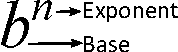
\includegraphics[width=0.7\textwidth]{img-02/potencia}
		\end{minipage}
		
		\begin{longtable}{|p{1.4in}|p{1.3in}|p{1.3in}|} \hline 
			\rowcolor{lightgray}\textbf{$b^{n}$} & \textit{$n$ parell} & \textit{$n$ imparell} \\ \hline 
			\cellcolor{lightgray}\textit{$b$ positiu} & \textbf{+} & \textbf{+} \\ \hline 
			\cellcolor{lightgray}\textit{$b$ negatiu} & \textbf{+} & \textbf{--} \\ \hline 
		\end{longtable}
		
	\end{theorybox}
\end{center}

\begin{mylist}

\exer \mental Determina el signe de les potències:  a) ($-$1)${}^{9}$ \quad b) ${(-5)}^{12}$  \quad c) ($-$12)${}^{5}$ \quad   d) (--8)${}^{4}$ 
\answers{[Negatiu, Positiu, Negatiu, Positiu]}

\exer  \spen Calcula el valor numèric de les potències
\begin{tasks}(2)
 \task ${\left(-3\right)}^4=$ 
 
 \task ${\left(-2\right)}^3=$ 
 
 \task ${\left(-1\right)}^{415}=$ 
 
 \task $\ {\left(-4\right)}^1=$
 
 \end{tasks}
\answers[cols=2]{[$81$, $-8$, $-1$, $-4$]}
  
\end{mylist}

\begin{example}
 \textbf{Potència de base racional: }Com calculam la potència quan la base és una fracció?

    S'eleva el numerador i el denominador a l'exponent ${\left(\frac{3}{5}\right)}^2=\frac{3^2}{5^2}=\ \frac{9}{25}$
\end{example}


\begin{mylist}
\exer \spen Calcula el valor numèric de les potències
\begin{tasks}(2)
\task  ${\left(\frac{3}{2}\right)}^4=$   \task ${\left(\frac{1}{5}\right)}^3=$  \task ${\left(-\frac{9}{4}\right)}^0=$  \task $\ {\left(\frac{-3}{4}\right)}^3=$
 \end{tasks}
\end{mylist}
\answers[cols=2]{[$\dfrac{81}{16}$, $\dfrac{1}{125}$, $1$, $-\dfrac{27}{64}$]}

\begin{theorybox}
 \textbf{Elevar un nombre a $-1$}: Significa calcular la inversa del nombre, per exemple
\[{\mathrm{3}}^{\mathrm{-}\mathrm{1}}\mathrm{=}\frac{\mathrm{1}}{\mathrm{3}};   \quad\quad\quad\quad  {\left(\frac{\mathrm{3}}{\mathrm{5}}\right)}^{\mathrm{-}\mathrm{1}}\mathrm{=}\frac{\mathrm{5}}{\mathrm{3}}\] 
\end{theorybox}

\begin{mylist}

\exer \spen Calcula el valor numèric de les potències
\begin{tasks}(2)
\task  ${\left(-3\right)}^{-1}=$   \task $2^{-1}=$   \task ${\left(-\frac{1}{4}\right)}^{-1}=$   \task $\ {\left(\frac{4}{7}\right)}^{-1}=$
\end{tasks}
\answers[cols=2]{[$-\dfrac{1}{3}$, $\dfrac{1}{2}$, $-4$, $\dfrac{7}{4}$]}
\end{mylist}


\begin{theorybox}

 \textbf{Potència d'exponent negatiu: }Què significa elevar a un exponent negatiu?

 Primer elevam a $-1$ que significa fer la inversa de la base, després elevam a l'exponent positiu:
\[{\mathrm{3}}^{\mathrm{-}\mathrm{2}}\mathrm{=}\frac{\mathrm{1}}{{\mathrm{3}}^{\mathrm{2}}}=\frac{1}{9}     ; \quad\quad\quad\quad {\left(\frac{\mathrm{3}}{\mathrm{5}}\right)}^{\mathrm{-}\mathrm{2}}\mathrm{=}{\left(\frac{\mathrm{5}}{\mathrm{3}}\right)}^{\mathrm{2}}=\frac{5^2}{3^2}=\frac{25}{9}\] 

\end{theorybox}

\begin{mylist}
\exer \spen Calcula el valor numèric de les potències
\begin{tasks}(2)
 \task ${\left(-3\right)}^{-3}=$  \task $2^{-4}=$   \task ${\left(-\frac{1}{4}\right)}^{-2}=$  \task$\ {\left(\frac{4}{7}\right)}^{-3}=$
\task $\left(\frac{5}{4}\right)^{3}$ =  \task $-\left(\frac{2}{7}\right)^{-4}$ =  
\task $\left(-\frac{1}{6}\right)^{4}$ = \task $\left(-\frac{5}{2}\right)^{-2}$ =
 \end{tasks}
\end{mylist}
\answers{[$-\dfrac{1}{27}$, $\dfrac{1}{16}$, $16$, 
	$\dfrac{343}{64}$, $\dfrac{125}{64}$, $-\dfrac{2041}{16}$, $1296$, $\dfrac{4}{25}$]}


\begin{theorybox}[Propietats de les potències]
\begin{minipage}[t]{0.82\textwidth}
	 \begin{tabular}{p{0.4\textwidth}p{0.6\textwidth}}
\textbf{Producte d'igual base:}  & ${\mathrm{b}}^{\mathrm{n}}\mathrm{\textrm{·}}{\mathrm{b}}^{\mathrm{m}}\mathrm{=\ }{\mathrm{b}}^{\mathrm{n+m}}$ \\ [0.25cm]

\textbf{Quocient d'igual base:}  & ${\mathrm{b}}^{\mathrm{n}}\mathrm{:}{\mathrm{b}}^{\mathrm{m}}\mathrm{=}\frac{{\mathrm{b}}^{\mathrm{n}}}{{\mathrm{b}}^{\mathrm{m}}}\mathrm{=\ }{\mathrm{b}}^{\mathrm{n-m}}$
\\[0.25cm]
\textbf{Potència de potencia:    } & ${{\mathrm{(b}}^{\mathrm{n}}\mathrm{)}}^{\mathrm{m}}\mathrm{=\ }{\mathrm{b}}^{\mathrm{n\textrm{·}m}}$
\\[0.25cm]
\textbf{Operacions d'igual exponent:} & ${\mathrm{a}}^{\mathrm{n}}\mathrm{\textrm{·}}{\mathrm{b}}^{\mathrm{n}}\mathrm{=\ }{\left(\mathrm{a\textrm{·}b}\right)}^{\mathrm{n}}$ \quad\quad ${\mathrm{a}}^{\mathrm{n}}\mathrm{:}{\mathrm{b}}^{\mathrm{n}}\mathrm{=\ }{\left(\mathrm{a:b}\right)}^{\mathrm{n}}$
\end{tabular}
\end{minipage}
\fbox{
\begin{minipage}{0.13\textwidth}
	\centering
	\textbf{Recorda:}
	\par
		
		$b^0=1$
		
		$b^1= b$
	
\end{minipage}
}
\end{theorybox}

\begin{mylist}
\exer \spen Expressa en forma d'una única potència:  

\begin{tasks}(2)
\task   ($-$7)${}^{3}$ · ($-$7)${}^{5}$ · ($-$7)${}^{2}$ · ($-$7)${}^{6 }$=    \task   3${}^{2}$ · 3${}^{7}$ · 3 · 3${}^{4}$ · 3${}^{3}$${}^{ }$=

 \task   ($-$6)${}^{4}$ · ${4}^{4}$ · ($-$1)${}^{4}$ · ($-$5)${}^{4}$=   \task  ($-$8)${}^{9}$: ($-$8)${}^{3}$  =

\task   ($-$3)${}^{2}$ :  ($-$3)${}^{7}$ =    \task   (+75)${}^{4}$ : ($-$3)${}^{4}$  =  

 \task  ($-$5)${}^{8}$ : ${8}^{8}$=    \task   (($-$2)${}^{5}$)${}^{6}$${}^{ }$=
\answers{[$(-7)^{16}$, $3^{17}$, $120^4$, $8^6$, $(-3)^{-3}$, $(-25)^4$, $(-5/8)^8$, $(-2)^{30}$]}


 \end{tasks}


\exer  Expressa com a única potència d'exponent positiu:  

\begin{tasks}(2)
\task  (\textbf{$-$}3/4)${}^{3}$ · (\textbf{$-$}3/4)${}^{2}$ · (\textbf{$-$}3/4)\textbf{${}^{-}$}${}^{8}$ =  \task   (1/8)\textbf{${}^{-}$}${}^{5}$· (1/8)${}^{4}$·(1/8)${}^{-}$${}^{2}$${}^{ }$=
\task   (5/4)${}^{6}$ · (\textbf{$-$}2/3)${}^{6}$· (\textbf{$-$}1/7)${}^{6}$ =  \task   (\textbf{$-$}3/5)${}^{-}$${}^{4}$ · (\textbf{$-$}3/8)${}^{-}$${}^{4}$ · (\textbf{$-$}1/4)\textbf{${}^{-}$}${}^{4}$${}^{ }$=
 \task   ($-$2/5)${}^{4}$ : ($-$2/5)${}^{7}$ =   \task    (5/8)${}^{3}$ : (5/8)${}^{-}$${}^{2}$${}^{ }$=
 \task    (1/5)${}^{-}$${}^{3}$ : (2/9)${}^{-}$${}^{3}$ =    \task    ($-$6)${}^{5}$ : (-2/9)${}^{5}$${}^{ }$=
\end{tasks}
 \answers{[$\left(-\frac{4}{3} \right)^{2}$, $\left(\frac{1}{8} \right)^{-3}=8^3$, $\left(\frac{5}{42} \right)^6$, $\left(\frac{160}{9} \right)^4$, $\left(-\frac{5}{2} \right)^3$, $\left(\frac{5}{8} \right)^5$, $\left(\frac{10}{9} \right)^3$, $27^5$]}


\exer Expressa en forma d'única potència:
\begin{tasks}(2)
\task 2${}^{5 }$ · ( -3)${}^{5}$ · ($-$1)${}^{5 }=$    \task ($-$1)${}^{3}$ · ($-$1)${}^{8}$ · ${(-1)}^{5}=$ 
\task  4${}^{3}$ · ($-$2)${}^{3}$· ($-$1)${}^{3 }$· 5${}^{3}=$    \task ($-$5)${}^{2}$ · ($-$5)${}^{4}=$  
\task ($-$9)${}^{2}$ · 9${}^{3}$ · 9${}^{4}$ · 9=     \task ($-$18)${}^{4}$: ($-$3)${}^{4}=$   
\task ${6}^{5} : {6}^{2}=$     \task ($-$3)${}^{2}$: ($-$3)${}^{4}=$
\end{tasks}
\answers{[$6^5$, $1$, $40^3$, $5^6$, $9^{10}$, $6^4$, $6^3$, $(-3)^{-2}$]} 


\exer  Expressa en forma de potència d'exponent positiu:  
\begin{tasks}(2)
 \task ($-$4) ${}^{-}$${}^{3 }$     \task ${9}^{-}$${}^{3}$  \task ($-$2)${}^{5}$: ($-$2)${}^{9}$  \task $(-5) \cdot (-5)^{2} : (-5)^{6}$
\end{tasks}
\answers[cols=2]{[$\left(\frac{-1}{4}\right)^3$, $\left(\frac{1}{9}\right)^3$, $\left(\frac{1}{2}\right)^4$, $\left(\frac{-1}{5}\right)^3$]}

\exer  Expressa en forma d'única potència:
\begin{tasks}(2)
\task  $\left( \frac23 \right)^{3 } \cdot \left( \frac{-1}{5} \right)^{3} \cdot \left( \frac{-4}{9} \right)^{3} \cdot \left( \frac{1}{2} \right)^{3}$    

\task  
$\left( \frac{-1}{4} \right)^3\cdot \left( \frac{-1}{4} \right)^{-2}\cdot \left( \frac{-1}{4} \right)\cdot \left( \frac{-1}{4} \right)^4$

\task $\left( \left( \frac{-1}{3} \right)^4 \right)^{3/2} \cdot \left( \frac{2}{5} \right)^{6}$

\task  $\left( \frac{2}{5} \right)^{1/2}\cdot \left( \frac{2}{5} \right)^{3/4}\cdot \left( \frac{2}{5} \right)^{-1/6}$
%\task (7/8)${}^{3}$${}^{ }$: (1/6)${}^{3}$
\end{tasks}
\answers[cols=2]{[$\left(\frac{4}{135}\right)^3$, $\left(-\frac{1}{4}\right)^6$, $\left(\frac{-2}{15}\right)^6$, $\left(\frac{2}{5}\right)^{12/12}=\frac{2}{5}$]}
\end{mylist}



\section{Notació científica}

	
\begin{theorybox}
	\video[ytid=9JUpIa4ncWg]{158}{Potències de 10. Un zoom còsmic.}
	
	Un número escrit en notació científica és de la forma:
	\[ m \times \ 10^{e} \]
	on l'exponent $e$ s'elegeix perquè el nombre $m$, en valor absolut, sigui major o igual a 1 i menor que 10.
	
	Algunes potències de 10 importants
\begin{center}
	\renewcommand{\arraystretch}{1.2}
\begin{tabular}{|l|c|c|l|l|}
	\hline
	\rowcolor{lightgray} Distància (m) & Ordre & Símbol & Exemple \\
	\hline
	1000000000000 & $10^{12}$ & tera (T) & Distància de Saturn al Sol\\
	\hline
	1000000000 & $10^9$ & giga (G) & Radi del Sol \\
	\hline
	1000000 & $10^6$ & mega (M) & Radi de la Lluna \\
	\hline
	1000 & $10^3$ & kilo (k) & 1 km \\
	\hline
	1 & $10^0$ &  & 1 m \\
	\hline
	0,001 & $10^{-3}$ & mil·li (m) & Gruix d'un cabell \\
	\hline
	0,000001 & $10^{-6}$ & micro ($\mu$) & Cèl·lula \\
	\hline
	0,000000001 & $10^{-9}$ & nano (n) & Mol·lècula \\
	\hline
		0,000000000001 & $10^{-12}$ & pico (p) & Àtom \\
	\hline
\end{tabular} 
\end{center}
\end{theorybox}
 

\begin{blueshaded}
	
	\begin{minipage}{0.7\textwidth}
		\textbf{Notació científica amb la calculadora:}
		
		Per trobar el valor decimal d'una arrel necessitaràs una calculadora científica, com ara la de la figura. Tot seguit et mostram alguns exemples
		
		\begin{tabular}{lrl}
			$1,25\cdot 10^3$:  & \tecla{\quad$1.25$\quad}  \tecla{\quad EXP\quad}  \tecla{\quad$3$\quad}   \tecla{\quad=\quad} & \pantalla{1250} \\ [0.25cm] 
			$2,4\cdot 10^{-2}$:  & \tecla{\quad$2.4$\quad}  \tecla{\quad EXP\quad}  \tecla{\quad$-2$\quad}   \tecla{\quad=\quad} & \pantalla{0.024} \\ [0.25cm] 
		\end{tabular}
	  
	  \vspace{0.25cm}
	  La tecla \tecla{ENG} permet passar de notació normal a científica i viceversa, per exemple:
	  
	  	\begin{tabular}{lrl}
	  	$1250000$:  & \tecla{\quad$1250000$\quad}  \tecla{\quad=\quad}  \tecla{\quad ENG\quad}   & \pantalla{$1.25\times 10^{6}$} \\ [0.25cm] 
	  	$2,5\cdot 10^{-3}$:  & \tecla{\quad$2.5$\quad}  \tecla{\quad EXP \quad}  \tecla{\quad -3 \quad}   \tecla{\quad = \quad} & \\
	  	& \tecla{\quad SHIFT \quad}  \tecla{\quad ENG \quad}     & \pantalla{$0.0025\times 10^{0}$} \\ [0.25cm] 
	  \end{tabular}
		
	\end{minipage}
	\begin{minipage}{0.3\textwidth}
		\centering
		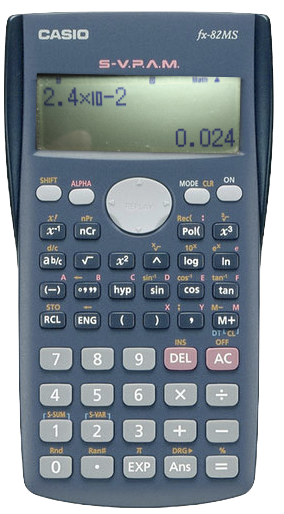
\includegraphics[width=0.9\textwidth]{img-02/fx82ms-a}
	\end{minipage}
	
	
	
\end{blueshaded}

\begin{mylist}

\exer \spen Expressa en notació científica:
\begin{tasks}(2)
\task 140000000 =    \task  32800 =  
\task  71000000000000000 =    \task  0,0000075 =
\task  $-$18000000 =     \task  0,00000000042 =
\task  $-$0,009 =    \task  0,00000000007 =
\end{tasks}
 \answers{[$\cient{1.4}{8}$, $\cient{3.28}{4}$, $\cient{7.1}{16}$, $\cient{7.5}{-6}$, $\cient{-1.8}{7}$, $\cient{4.2}{-10}$, $\cient{-9}{-3}$, $\cient{7}{-11}$]}

\exer  \simbolsearch Cerca informació expressada en notació científica sobre:
\begin{tasks}(2)
\task  La distància entre la Terra i la Lluna  \task  Unitat de massa atòmica
\task  Km que corresponen a un any llum  \task  Un gúgol   
\end{tasks}
\answers[cols=2]{[$\cient{3.84}{8}$ m, $\cient{1.66}{-27}$ kg, $\cient{9.46}{12}$ km, $\cient{10}{100}$]}


\exer[1]  Realitza les operacions i expressa el resultat en notació científica:
\begin{tasks}(2)
\task 4 · 10${}^{3}$ + 2,4 · 10${}^{6}$ -- 1,7 · 10${}^{5}$ -- 3 · 10${}^{3}$ \task 2,3 · 10${}^{-}$${}^{5}$ -- 3,45 · 10${}^{-}$${}^{4}$ + 6 · 10${}^{-}$${}^{3}$
\task  3 · 10${}^{-}$${}^{4}$ · 4,5 · 10${}^{2 }$   \task  1,8 · 10${}^{5}$: 5 · 10${}^{8}$
\end{tasks}
\answers[cols=2]{[$2.231\cdot 10^6$, $5.678\cdot 10^{-3}$, $1.35\cdot 10^{-5}$, $3.6\cdot 10^{-4}$]}


\exer[1]  L'estel Sirius està a uns 8,611 anys llum del nostre planeta. Expressa en metres, mitjançant notació científica la distància que recorreria una nau espacial que realitzés un trajecte d'anada i tornada a Sirius. (\textit{Recorda}: Un any llum, la longitud que recorre la llum en un any, és aproximadament igual a  9,46~$\times$~10${}^{12}$~km (9~460~730~472~580,8~km amb més aproximació))
\answers{$1.629\cdot 10^{17}$ m}

 

\vspace{-2cm}
\exer[1]  \begin{minipage}[t]{0.7\textwidth}  La massa d'un electró en repòs s'estima en 9,11 · 10${}^{-31}$ kg, la d'un protó és d'1,672 $\cdot$ 10${}^{-}$${}^{27}$ kg, i la d'un neutró 1,64 x 10${}^{-}$${}^{27}$ kg. Calcula la massa d'un àtom de carboni 14 (C${}_{14}$) format per sis protons, sis electrons i 6 + 2 = 8 neutrons. (El C${}_{14}$ és un isòtop que té dos neutrons més que el carboni normal i que s'utilitza per datar).
\end{minipage}
\begin{minipage}{0.3\textwidth}
\centering
\vspace{2cm}
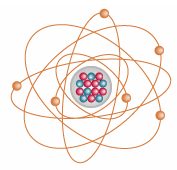
\includegraphics[width=0.6\textwidth]{img-02/carbono14}
\end{minipage}
\answers{La massa de l'isòtop C${}_{14}$ és: $6\times 1,672 \cdot 10^{-27} + 6 \times 9,11 \cdot 10^{-31}+ 8\times 1,64 \cdot 10^{-27}  = 2.32\cdot 10^{-26}$ kg}

 
\vspace{3cm}

\exer  Calcula i expressa en notació científica:
\begin{tasks}(2)
 \task 0,00829 + 4 · 10${}^{-}$${}^{3}$ + 7,45 · 10${}^{-}$${}^{5}$      \task 5 · 10${}^{6}$ -- 2,8 · 10${}^{7}$ -- 3 · 10${}^{5}$
 \task 5 · 10${}^{-}$${}^{2}$ -- 4 · 10${}^{2}$ + 1,4 · 10${}^{-}$${}^{3}$     \task 3 · 10${}^{-}$${}^{5 }$ · (-- 2,7) · 10${}^{-}$${}^{3}$ + 4,2 · 10${}^{-}$${}^{6}$
\end{tasks}
\answers[cols=2]{[$\cient{1.236}{-2}$, $\cient{-2.33}{7}$, $\cient{-3.99}{2}$, $\cient{4.12}{-6}$]}
 


\exer[1]  S'estima que existeixen 40 milions de bacteris en un gram de terra. Expressa en notació científica de forma aproximada el nombre de bacteris que existeixen en uns camions que estan descarregant 50 tones mètriques d'arena en una platja.
\answers{$50 t \cdot \frac{1\,000\,0000 \text{ g}}{1 t} \cdot \frac{40\cdot 10^6 \text{ bacteris}}{1 \text{ g}}=4\cdot 10^{13}$ bacteris}

 


\exer  Si  \textit{x} = 240000; \textit{y =} 0,00058; \textit{z }= 7,2 · 10${}^{6}$: Calcula i expressa en notació científica 
\begin{tasks}(3)
 \task \textit{x·y}      \task 2\textit{x }+ \textit{y}·10${}^{7}$      \task 3\textit{x} -- 5\textit{y}
\end{tasks}
\answers{[$\cient{1.392}{2}$, $\cient{4.86}{5}$, $\cient{7.2}{5}$]}


\exer[1]  Arquimedes, en el seu tractat \textit{El arenario} explica una manera per expressar nombres molt grans, com el nombre de grans d'arena que hi ha en tota la Terra. Anem a estimar-los ara per un altre procediment. Estimem quants grans d'arena necessitem per tenir un gram. Suposa que 50 grans d'arena. S'estima que la massa de la Terra és de:  $M_T$=5 980 000 000 000 000 000 000 000 000 g = 598 \textbf{$\boldsymbol{\cdot}$} 10${}^{25}$ g

 Calcula de forma aproximada el nombre de grans d'arena que hi ha en tota la Terra.
 
\answers{$ 598 \cdot 10^{25} \text{ g} \cdot \frac{50 \text{ grans}}{1 \text{ g}} \approx 3\cdot 10^{29}$ grans d'arena}


 

\vspace{-2cm}
\exer  \begin{minipage}[t]{0.7\textwidth}
	\simbolsearch Cerca a Wikipèdia les masses i els radis dels planetes Júpiter i la Terra
	 % que la massa de Júpiter és d'1,898·10${}^{27}$ kg, i que la massa de la Terra és de 5,972·10${}^{24}$ kg.
	\begin{tasks}
	\task Calcula la relació de massa entre Júpiter i la Terra.
	%
	\task Quants de planetes Terra necessitam per ocupar el mateix volum que el planeta Júpiter? $V=\ofrac{4}{3}\pi R^3$
	%
	\task Calcula la relació de densitat ($d=M/V$) entre Júpiter i la Terra.
	\end{tasks}
	\answers{$M_J=1,898$·$10^{27}$ kg, $M_T=5,972$·$10^{24}$ kg, $R_J=69911$ km, $R_T=6371$ km, \par a) $\dfrac{M_J}{M_T} = 318$,\par b) $\dfrac{V_J}{V_T} = 1321$,   $\dfrac{d_J}{d_T} = 0.24$\par és un planeta gasós (de fet és menys dens que l'aigua).}
	
\end{minipage}
\begin{minipage}{0.3\textwidth}
	\centering
	\vspace{2cm}
	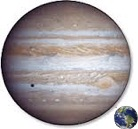
\includegraphics[width=0.6\textwidth]{img-02/jupiter}
\end{minipage}





\exer  Utilitza la calculadora per obtenir la teva edat expressada en segons en notació científica.
\answers{14 anys=$\cient{4.42}{8}$ s;\par 15 anys=$\cient{4.73}{8}$ s;\par 16 anys=$\cient{5.05}{8}$ s}

 


\exer  S'estima que el volum de l'aigua dels oceans és de 1~285~600~000 km${}^{3}$ i el volum d'aigua dolça és de 35~000~000 km${}^{3}$. Escriu aquestes quantitats en notació científica i calcula la proporció d'aigua dolça.
\answers{$\cient{1.2856}{9}$ km${}^{3}$ i $\cient{3.5}{7}$ km${}^{3}$.\par La proporció és 2.72 \%}

 


\exer  Se sap que en un àtom d'hidrogen el nucli constitueix el 99 \% de la massa, i que la massa d'un electró és aproximadament de  $9,109 \cdot 10^{-31}$ kg. Quina massa té el nucli d'un àtom d'hidrogen? (\textit{Recorda}: Un àtom d'hidrogen està format pel nucli, amb un protó, i per un únic electró).
\answers{Si tenim present que l'electró, que pesa 9,109 $\cdot$ 10${}^{-}$${}^{31}$ kg, representa únicament l'1 \%, només cal multiplicar per 100 i obtenim la massa de l'àtom: $\cient{9.109}{-29}$ kg}

 


\exer  A ne'n Joan li han fet una analítica de sang i té 5 milions de glòbuls vermells en cada mm${}^{3}$. Escriu en notació científica el nombre aproximat de glòbuls vermells que té en Joan estimant que té 5 litres de sang. (1 l=1 dm$^3$)
\answers{En Joan té $\cient{2.5}{9}$ glòbuls vermells}

\end{mylist}

\pagebreak
\section{Arrels o radicals}

\begin{theorybox}
	\begin{minipage}{0.35\textwidth}
		\centering
		\videonw[ytid=oIk7H9wenrM]{128}{Arrels: Definició}
	\end{minipage}
\begin{minipage}{0.35\textwidth}
	\centering
	\videonw[ytid=UTYWwJAcJfE]{130}{Radicals: Propietats}
\end{minipage}
\begin{minipage}{0.2\textwidth}
	\centering
	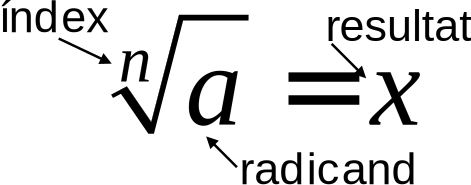
\includegraphics[width=0.9\textwidth]{img-02/radical}
\end{minipage}

\begin{center}
\begin{tabular}{llll}
Deim que l'arrel quadrada & $\sqrt{16}=4$ & perquè & $4^2 = 16$ \\
Deim que l'arrel cúbica  & $\sqrt[3]{125}=5$& perquè& $5^3 = 125$\\
Deim que l'arrel quarta  & $\sqrt[4]{16}=2$ &perquè& $2^4 = 16$\\
$\cdots$ & & & \\
En general l'arrel enèsima &$\sqrt[n]{a}=x$& perquè &$x^n = a$
\end{tabular}
\end{center}
\end{theorybox}

\begin{mylist} 


\exer  \spen  Escriu la llista dels 10 primers quadrats perfectes. 


\begin{longtable}{|p{0.5in}|p{0.3in}|p{0.3in}|p{0.3in}|p{0.3in}|p{0.3in}|p{0.3in}|p{0.3in}|p{0.3in}|p{0.3in}|p{0.3in}|} \hline 
\textbf{$n$} & 1 & 2 & 3 & 4 & 5 & 6 & 7 & 8 & 9 & 10 \\ \hline 
\textbf{$n^{2}$} &  &  &  &  &  &  &  &  &  &  \\ [0.5cm] \hline 
\end{longtable}
\answers{1, 4, 9, 16, 25, 36, 49, 64, 81, 100}

 
 \exer \mental  Calcula \textbf{mentalment} les següents arrels:
 \begin{tasks}(7)
 	\task  $\sqrt{49} $ \task  $\sqrt{25} $  \task  $\sqrt{100} $  \task  $\sqrt{64} $ \task $\sqrt{81} $  \task  $\sqrt{1} $   \task  $\sqrt{0} $
 \end{tasks}
\answers[cols=2]{[7, 5, 10, 8, 9, 1, 0]}
 
 \exer  \mental Calcula \textbf{mentalment} la part entera de les següents arrels:
 \begin{tasks}(7)
 	\task  $\sqrt{51} $ \task  $\sqrt{27} $  \task  $\sqrt{102} $  \task  $\sqrt{63} $ \task  $\sqrt{80} $  \task  $\sqrt{2} $            \task  $\sqrt{123} $
 \end{tasks}
 \answers[cols=2]{[7, 5, 10, 7, 8, 1, 11]}

 
 \end{mylist}

\vspace{0.5cm}

\begin{blueshaded}
	
	\begin{minipage}{0.7\textwidth}
		\textbf{Arrels amb la calculadora:}
		
		Per trobar el valor decimal d'una arrel necessitaràs una calculadora científica, com ara la de la figura. Tot seguit et mostram la combinació de tecles que has d'utilitzar.
		
		\begin{tabular}{lrl}
			$\sqrt[3]{5}$:  & \tecla{SHIFT}   \tecla{\quad$x^3$\quad}  \tecla{\quad5\quad}    \tecla{\quad=\quad} & \pantalla{1.709975947} \\ [0.25cm]
			$\sqrt[4]{3}$:  & \tecla{\quad4\quad}  \tecla{SHIFT}   \tecla{\quad$\wedge$\quad}  \tecla{\quad 3\quad}    \tecla{\quad=\quad} & \pantalla{1.316074013} 
		\end{tabular}
		
		\vspace{0.25cm}
		Les comprovacions de cada arrel són:
		
		
		\begin{tabular}{lrl}
			$1.709975947^3$:  & \tecla{1.709975947}   \tecla{\quad$\wedge$\quad}  \tecla{\quad3\quad}    \tecla{\quad=\quad} & \pantalla{5} \\ [0.25cm]
			$1.316074013^4$:  & \tecla{1.316074013}   \tecla{\quad$\wedge$\quad}  \tecla{\quad 4\quad}    \tecla{\quad=\quad} & \pantalla{3} 
		\end{tabular}
		
		
	\end{minipage}
	\begin{minipage}{0.3\textwidth}
		\centering
		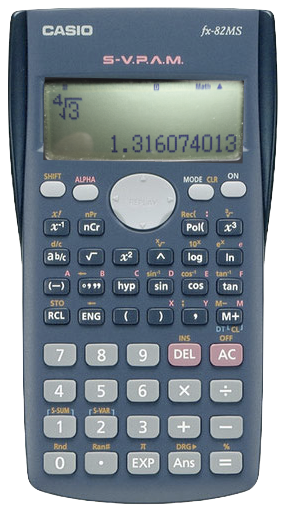
\includegraphics[width=0.9\textwidth]{img-02/fx82ms-b}
	\end{minipage}
	
	
	
\end{blueshaded}


\begin{theorybox}

\begin{center}
	\begin{tabular}{l|c|c}
		 Signe de $\sqrt[n]{a}$ & $a>0$ & $a<0$ \\ \hline
		 $n$ parell & $+$ & No existeix \\ \hline
		 $n$ senar & $+$ & $-$
	\end{tabular}
\end{center}
\end{theorybox}


\begin{mylist}
  \exer \mental Indica quines arrels quadrades són nombres enters, quines nombres irracionals i quines no existeixen:
 \begin{tasks}(4)
 	\task  $\sqrt{36} $ \task  $\sqrt{-25} $  \task  $\sqrt{100} $ \task  $\sqrt{32} $ \task  $\sqrt[5]{-7} $  \task  $\sqrt{10} $            \task  $\sqrt{100}$ \task $\sqrt[3]{-125}$
 \end{tasks}
\answers{[entera, no, natural, irracional, irracional, irracional, entera, entera]}

 \exer  Calcula totes les solucions:  
 \begin{tasks}(5)
 	\task  $\sqrt{121} $   \task  $\sqrt[{3}]{-8} $  \task  $\sqrt[{4}]{10000} $  \task  $\sqrt[{5}]{-1} $      \task  $\sqrt[{7}]{1} $
 \end{tasks}
\answers{[$\pm 11$, --2, $\pm 10$, --1, 1]}
 
\end{mylist}

 \begin{theorybox}
  Tot radical o arrel es pot expressar com a potència d'exponent una fracció:
  $\sqrt[3]{5^2} = 5^{\ofrac{2}{3}}$
  
  i viceversa $2^{\ofrac{5}{4}}=\sqrt[4]{2^5}$. Fixeu-vos que l'índex de l'arrel és el denominador de l'exponent.
 \end{theorybox}
 
 \begin{mylist}
 	
 \exer \spen  Expressa en forma de radical:  
 \begin{tasks}(3)
 	\task  ($-$3)${}^{4/5}=$  \task  8${}^{1/3}=$   \task  5${}^{2/3}=$
 \end{tasks}
 \answers{[$\sqrt[5]{(-3)^4}$, $\sqrt[3]{8}$, $\sqrt[3]{5^2}$]}
 
 \exer \spen Expressa en forma d'arrel: 
 \begin{tasks}(4)
 	\task  ($-$4)${}^{3/5}=$  \task  7${}^{1/6   }=$ \task ${21}^{1/3 }=$  \task  ($-$5)${}^{2/3}=$
 \end{tasks}
\answers{[$\sqrt[5]{(-4)^3}$, $\sqrt[6]{7}$, $\sqrt[3]{21}$, $\sqrt[3]{(-5)^2}$]}
 
 \exer \spen  Expressa en forma de potència:  
 \begin{tasks}(4)
 	\task  $\sqrt[{5}]{6^{3} } $${}^{ }=$\task  $\sqrt{(-7)^{5} }=$ \task  $\sqrt{3^{5} }=$ \task  $\sqrt[{3}]{(-30)^{4} }=$
 \end{tasks}
\answers{[$6^{3/5}$, $(-7)^{5/2}$, $3^{5/2}$, $(-30)^{4/3}$]}
 
 \exer  Calcula: 
 \begin{tasks}(5)
 	\task  $\sqrt{12100} $  \task  $\sqrt{0,64}$   \task  $\sqrt[3]{-0,008}$  \task  $\sqrt[{5}]{-1} $  \task  $\sqrt{0,49} $
 \end{tasks}
\answers{[110, 0.8, --0.2, --1, 0.7]}
 
 \exer  Calcula: 
 \begin{tasks}(4)
 	\task  $\sqrt[{4}]{2,0736} $ \task  $\sqrt[{5}]{-0,00001} $${}^{ }$\task  $\sqrt{33640000} $  \task   $\sqrt[{3}]{-2,7\cdot 10^{-5} } $
 \end{tasks}

\answers{[1.2, --0.1, 5800, --0.03]}

\end{mylist}

\begin{theorybox}[Operacions amb radicals]
\textbf{Suma i resta:} Tan sols podem sumar i restar radicals idèntics
\[\boxed{2\sqrt{5} + 4 \sqrt{5}} - 7\sqrt{3}  = \boxed{ 6\sqrt{5} } - 7\sqrt{3}\]

\textbf{Producte i divisió de radicals d'igual índex:} 
\[ \sqrt{5}\cdot \sqrt{3} = \sqrt{15},  \quad\quad\quad \quad\quad\quad \frac{\sqrt{8}}{\sqrt{2}} = \sqrt{\frac{8}{2}}=\sqrt{4}=2 \]
\end{theorybox}

\vspace{2cm}
\begin{mylist}
 \exer  \spen Redueix:  
 \begin{tasks}(2)
 	\task  $3\sqrt{2} - 2\sqrt{2} + 7 \sqrt{2}=$  
 	
 	\task  $\frac{1}{2}\sqrt{5} + 3\sqrt{5} + \sqrt{5}=$  
 	
 	\task  $\sqrt{2} - 2\sqrt{3} + \frac{3}{4} \sqrt{2}=$
 	
 	\task  $-5\sqrt{7} + 3\sqrt{7} + 3 \sqrt{3}=$
 \end{tasks}
\answers[cols=2]{[$8\sqrt{2}$, $\frac{9}{2}\sqrt{5}$, $\frac{7}{4}\sqrt{2}-2\sqrt{3}$, $-2\sqrt{7}+3\sqrt{3}$]}

\end{mylist} 

\begin{theorybox}[Extreure factors d'un radical]
 En principi, les arrels $\sqrt{5} + \sqrt{20}$ no es poden ajuntar en una perquè són diferents. No obstant això, podem simplificar $\sqrt{20}$ extraient factors. 
 
 El primer que feim és \textbf{descomposar} el nombre en factors primers: $20 = 2^2 \cdot 5$
 
 \[ \sqrt{20} = \sqrt{ \boxed{2^2} \cdot 5} = \boxed{2} \sqrt{5} \]
 

``{  \normalfont \textit{tot el que està elevat a 2 dins una arrel quadrada surt defora de l'arrel sense l'exponent}}"
 
\end{theorybox}

\begin{resolt}[E]{
 Extreu factors 
 
  \[ \text{a) } \sqrt[3]{2 \cdot 5^3 } \]

 \[\text{b) } 5\sqrt{2^5 \cdot 3^2 } \]

 \[\text{c) } \sqrt[4]{162 } \]

 \[\text{d) } \sqrt[3]{32} \]
}

a) Tot el que està elevat a 3 surt de l'arrel cúbica $ \sqrt[3]{2 \cdot 5^3 }=  5 \sqrt[3]{2}$
\vspace{0.25cm}


b) Tot el que està elevat a 2 surt de l'arrel quadrada. Feim ``paquets'' si l'exponent supera a 2:  $  5\sqrt{2^5 \cdot 3^2 } = 5\sqrt{2^2 \cdot 2^2 \cdot 2 \cdot 3^2}=5\cdot 2 \cdot 2 \cdot 3\sqrt{ 2} =12 \sqrt{2}$
\vspace{0.25cm}


c) Descomposam el radicand i treim factors $ \sqrt[4]{162 }= \sqrt[4]{2\cdot 3^4 }= 3 \sqrt[4]{2}$
\vspace{0.25cm}

d) Descomposam el radicand, feim ``paquets'' i treim factors  $ \sqrt[3]{32}=\sqrt[3]{2^5}=\sqrt[3]{2^3 \cdot 2^2}=2\sqrt[3]{2^2}$ 
\end{resolt}

\begin{mylist}
 \exer[1]  Extreu els factors possibles en cada radical:  
 \begin{tasks}(3)
 	\task  $\sqrt[{4}]{a^{6\cdot } b^{5} } $  \task  $\sqrt[{3}]{6^{5} \cdot 3^{4} \cdot 2^{6} } $  \task  $\sqrt{4\cdot 5^{3} \cdot 9^{3} } $
 \end{tasks}
 \answers[cols=2]{[$a\cdot b\,\sqrt[4]{a^2 b}$, $6^2 \cdot 3 \cdot 2^2 \sqrt[3]{3\cdot 6^2}$, $90\,\sqrt{45}$]}
 
 \exer[1]  Extreu factors de cada radical: 
 \begin{tasks}(2)
 	\task  $\sqrt[{3}]{5^7} $   \task  $\sqrt{54} $    \task  $\sqrt{\frac{8}{9} } $        \task $\sqrt{\frac{x^{3} }{y^4} } $
 \end{tasks}
\answers[cols=2]{[$5^3\,\sqrt[{3}]{5}$, $3\sqrt{6}$, $\frac{2}{3}\sqrt{2}$, $\frac{x}{y^2}\sqrt{x }$]}
\end{mylist}

\pagebreak

 \begin{theorybox}[Arrel d'una arrel]
 	Una forma de calcular l'arrel d'una arrel és passar-les a forma de potència i operar les potències. Per exemple:
 	\[ \sqrt[3]{ \sqrt[4]{5} } = \left(5^\ofrac{1}{4}\right)^\ofrac{1}{3} =  \left(5 \right)^\ofrac{1}{12} = \sqrt[12]{5}  \]
 	
 	Una forma més còmoda i ràpida és simplement escriure una arrel d'índex el producte d'índexs:
 	
 	\[ \sqrt[n]{ \sqrt[m]{a} } =  \sqrt[n\cdot m ]{a}  \]
 	
 	
 	
\includegraphics[width=0.75cm]{img-02/warning}  \textbf{Recorda que una arrel quadrada conté un índex 2:  $\sqrt{a}=\sqrt[ {\small 2}]{a}$}
 \end{theorybox}



\begin{mylist} 
 \exer  Expressa en forma d'única arrel:   
 \begin{tasks}(2)
 	\task  $\sqrt[{3}]{\sqrt{18} } $   \task  $\sqrt[{4}]{\sqrt[{3}]{25} } $
 \end{tasks}
\answers{[$\sqrt[6]{18}$, $\sqrt[12]{25}$]}
 
 \exer  Opera expressant prèviament en forma de potència:  
 \begin{tasks}(2)
 	\task  $\sqrt[{4}]{2^{3} } \cdot \sqrt{2^{5} } $   \task  $\frac{\sqrt[{3}]{5} \cdot \sqrt[{4}]{5^{2} } }{\sqrt{5^{3} } } $
 \end{tasks}
\answers{[$2^{13/4}=\sqrt[4]{2^{13}}$, $5^{-2/3}=\sqrt[3]{5^{-2}}$]}
 
 \exer  Simplifica l'expressió (passa primer en forma de potència):   
 \begin{tasks}(2)
 	\task  $\left(\frac{x^{\ofrac{2}{3} } }{\sqrt{x} } \right)^{3} $   \task  $\frac{\sqrt{x^{3} } \cdot \sqrt[{5}]{x^{11} } }{\sqrt[{3}]{x} } $
 \end{tasks}
 \answers{[$x^{1/2}=\sqrt{x}$, $x^{101/30}=\sqrt[30]{x^{101}}$]}
 
 \exer  Extreu tots els possibles factors d'aquests radicals:
 \begin{tasks}(4)
 	\task \textbf{ $\sqrt{3^{3} \cdot 10^{5} \cdot 2} $}  \task  \textbf{$\sqrt[{3}]{6^{9} \cdot 2^{5} } $}${}^{  }$\task  \textbf{$\sqrt[{4}]{x^{11} \cdot y^{5} } $}${}^{  }$\task  \textbf{$\sqrt[{3}]{3^{4} \cdot 5^{6} } $}
 \end{tasks}
\answers[cols=2]{[$300\,\sqrt{60}$, $432\,\sqrt[3]{4}$, $x^2 y\,\sqrt[4]{x^3 y}$, $75\,\sqrt[3]{3}$]}
 
 \exer  Extreu els factors possibles d'aquests radicals:
 \begin{tasks}(4)
 	\task ${}^{ }$\textbf{$\sqrt[{3}]{a^{7} \cdot b^{3} \cdot c^{-6} } $ }${}^{ }$\task  \textbf{$\sqrt{5^{-5} \cdot 3^{-6} } $ } \task  \textbf{$\sqrt[{4}]{10^{5} :6^{8} } $}   \task  \textbf{$\sqrt{x^{3} \cdot x^{8} \cdot x} $}
 \end{tasks}
\answers[cols=2]{[$\frac{a^2 b}{c^2}\,\sqrt[3]{a}$, $\frac{1}{5^2 3^3}\,\sqrt{1/5}$, $\frac{10}{6^2}\,\sqrt[4]{10}$, $x^6$]}
 
 \exer  Simplifica:  
 \begin{tasks}(4)
 	\task  $\sqrt{\left(\frac{2}{5} \right)^{3} } $ \task  $\sqrt[{3}]{\left(\frac{-4}{5} \right)\cdot \left(\frac{-4}{5} \right)^{5} } $${}^{ }$\task  $\sqrt{\frac{x^{3} \cdot y^{4} }{x^{8} \cdot y} } $  \task  $\sqrt[{4}]{\left(\frac{1}{4} \right)^{5} :\left(\frac{4}{3} \right)^{5} } $
 \end{tasks}
\answers[cols=2]{[$\frac{2}{5} \sqrt{\frac{2}{5} } $, $\left(\frac{-4}{5} \right)^2$,  $\frac{y}{x^2} \sqrt{ \frac{y}{x}}$, $\frac{3}{16} \sqrt[4]{\frac{3}{16}}$]}
 
 \exer Expressa en forma d'única arrel:  
 \begin{tasks}(4)
 	\task  \textbf{$\sqrt{\sqrt{48} } $}   \task  \textbf{$\sqrt[{3}]{\sqrt{450} } $}${}^{  }$\task  \textbf{$\sqrt[{4}]{\sqrt[{3}]{9000} } $}  ${}^{ }$\task  \textbf{$\sqrt[{2}]{\sqrt[{5}]{-1} } $} 
 \end{tasks}
\answers[cols=2]{[$\sqrt[4]{48}$, $\sqrt[6]{450}$, $\sqrt[12]{9000}$, $\sqrt[10]{-1}=\nexists$]}
 
 \exer  Simplifica les operacions:  
 \begin{tasks}(3)
 	\task  $\sqrt[{3}]{3^{5} } \cdot \sqrt[{3}]{2^{4} } $${}^{ }$${}^{ }$\task  $\left(\sqrt[{3}]{-27} \right)\cdot 5^{\ofrac{2}{3} } $  \task  $\sqrt[{5}]{2^{12} } :\sqrt[{5}]{3^{8} } $  
 \end{tasks}
 \answers{[$6\,\sqrt[3]{18}$,   $-3\,\sqrt[3]{25}$,   $\frac{4}{3}\,\sqrt[5]{\frac{4}{27}}$]}
 
 \vspace{2cm}
 
 \exer  Simplifica les operacions:  
 \begin{tasks}(2)
 	\task  $\sqrt[{3}]{x^{5} } :\sqrt[{2}]{x^{3} } $   \task  $\sqrt{\sqrt{10^{12} } } $   \task  $\sqrt{5\cdot (-2)^{6} \cdot (-3)^{6} } $ \task  $\sqrt[{5}]{(-6)^{12} } :\sqrt[{5}]{(-6)^{7} \cdot 3^{10} } $ 
 \end{tasks}
\answers{[$\sqrt[6]{x^{19}}$, $10^3$, $6\,\sqrt[3]{5}$, $-\frac{1}{3}$]}
\end{mylist}

\begin{resolt}[E]{
	Operacions amb diferent índex:
	
	\[   \sqrt{3} \cdot \sqrt[3]{2}  \]
}
 Passam tots els radicals en forma de potència

\[ \sqrt{2} \cdot \sqrt[3]{2}= 2^{1/2} \cdot 2^{1/3} \]

tot seguit operam les potències

\[ =2^{1/2} \cdot 2^{1/3} = 2^{1/2+1/3} = 2^{5/6} \]

finalment, tornam a passar a forma d'arrel
$ 2^{5/6} = \sqrt[6]{2^5} $
\end{resolt}

\begin{mylist}
	\exer Opera passant prèviament en forma de potència:
	\begin{tasks}(3)
		\task $\sqrt{5^3} : \sqrt[3]{5}=$
		\task $\sqrt[4]{a^3} \cdot \sqrt[5]{a^2}=$
		\task $\sqrt{a} \cdot \sqrt{\sqrt{a}} : \sqrt[3]{a}=$ 
	\end{tasks}
\answers{[$\sqrt[6]{5^{11}}$, $\sqrt[20]{a^{23}}$, $\sqrt[12]{a^{5}}$]}
\end{mylist}

\vspace{0.25cm}
\begin{autoaval}{30}
\begin{mylist}
\exer[2] Calcula el valor numèric: a)\quad ($-$6)${}^{3}$ · ($-$6)${}^{-5}$ · ($-$6);  \quad b) \quad  ${12}^{7}$: ${12}^{5}$
%\begin{tasks}(3)
%	\task  6  \quad i  \quad 12${}^{2}$              \task  1/6  \quad i  \quad 12${}^{5        }$    \task  $-$1/6${}^{ }$  \quad i  \quad 12${}^{2}$  
%\end{tasks}
\answers{[$-\dfrac{1}{6}$, $144$]}

\exer[2]  Expressa com una potència:  a) \quad ($-$5)${}^{4}$ · ($-$1)${}^{4}$ · ${6}^{4}$;    \quad b)  \quad  $(-8)^7 : {5}^{7}$
%\begin{tasks}(3)
%	\task  ($-$30)${}^{4}$   \quad i  \quad  ($-$3)${}^{7}$         \task  30${}^{4}$  \quad i  \quad ($-$8/5)${}^{7}$         \task  30${}^{4}$  \quad i  \quad ($-$3)${}^{7}$
%\end{tasks}
\answers{[$30^4$, $\left(-\dfrac{8}{5}\right)^7$]}

\exer[2]  Expressa com una potència: a) (($-$2)${}^{5}$)${}^{3}$; \quad b)  \quad    (($-$1)${}^{5}$)${}^{7}$; \quad c)  \quad  (($-$5)${}^{2/3}$)${}^{6}$
%\begin{tasks}(3)
%	\task   ($-$2)${}^{15}$;  \, ($-$1)  \,i  \,  ${5}^{8/3}$  \task  $-$2${}^{15}$;\,  ($-$1) \,   i  \,  $-$5${}^{4}$    \task  ($-$2)${}^{15}$; \, ($-$1)    \, i  \,  ($-$5)${}^{4}$
%\end{tasks}
\answers{[$(-2)^{15}$, $-1$, $(-5)^{4}$]}

\begin{comment}
\exer  Calcula el valor numèric de: ${8}^{-3}$;   \, ($-$2)${}^{-4}$    \, i  \,   (10${}^{5}$)${}^{-2}$
\begin{tasks}(2)
	\task  1/512;\,      1/16  \,  i  \,   1/10${}^{10}$  \task 1/8${}^{3}$;  \,  - 1/2${}^{4}$  \, i  \,   1/10${}^{10}$
\end{tasks}
\end{comment}

\exer[2] Calcula el valor numèric: a) ( 5/3)${}^{-1}$; \, b)  (-1/3)${}^{-2}$;     \, c)      (- 2/5)${}^{-3}$
%\begin{tasks}(2)
%	\task  5${}^{3}$/7${}^{3}$;  \,    1/3${}^{2}$   \, i  \,   -2${}^{4}$/5${}^{4}$  \task  5${}^{3}$/7${}^{3}$;  \,  3${}^{2}$    \, i  \,   2${}^{4}$/5${}^{4}$
%\end{tasks}
\answers{[$\dfrac{3}{5}$, $9$, $-\dfrac{125}{8}$]}

\exer[2]  Simplifica: (2/3)${}^{3}$ · (2/3)${}^{2}$ ·  (2/3)${}^{-5}$
%\begin{tasks}(4)
%	\task   1   \task  2/3   \task  $-$2/3   \task  (2/3) · ($-$3/2)
%\end{tasks}
\answers{1}

\exer[2]  a) Converteix a notació habitual 3,1 · 10${}^{8}$  

 b) Passa a notació científica \quad 0,0000000095 
%\begin{tasks}(3)
%	\task   3100000000  \quad i  \par 9,5 · 10${}^{-10}$ \task   310000000  \quad i  \par 9,5 · 10${}^{-10  }$ \task   310000000  \quad i  \par 9,5 · 10${}^{-9}$
%\end{tasks}
\answers[cols=2]{[310000000, $9.5 \cdot 10^{-9}$]}

\exer[2]  Opera  (0,00098 + 3 · 10${}^{-6}$ -- 4,2 · 10${}^{-4}$) · 2,5 · 10${}^{5}$
%\begin{tasks}(4)
%	\task  124,5  \task  2407,5  \task  107,5   \task  140,75
%\end{tasks}
\answers{140.75}

\exer[2]  Aplica la definició de radical per esbrinar $n$: a) $\sqrt[3]{n}=-5 $; b) $\sqrt[n]{64}=8 $; c) $\sqrt[{5}]{-32}=n$
%\begin{tasks}(3)
%	\task  $-$11, 16, $-$1  \task  11, 16, 1  \task  $-$11, $-$16, $-$1
%\end{tasks}
\answers{[$n=-125$, $n=2$, $n=-2$]}

\exer[2]  Expressa en forma de radical i digues si es poden calcular o no: 

a) ($-$4)${}^{3/5}$ ; \, b) 3${}^{1/2}$;   \, c) \,  ($-$5)${}^{3/4}$
%\begin{tasks}(3)
%	\task  $\sqrt[{5}]{-4^{3} } $;\, $\sqrt{3} $  \, i  \,  $\sqrt[{3}]{-5^{4} } $  \task  $\sqrt[{5}]{\left(-4\right)^{3} } $; $\sqrt{3} $   i   $%\sqrt[{3}]{\left(-5\right)^{4} } $   \task  --$\sqrt[{5}]{4^{3} } $; \,$\sqrt{3} $  \, i  \,  $\sqrt[{3}]{-\left(5^{4} \right)} $
%\end{tasks}
\answers[cols=2]{[$\sqrt[{5}]{\left(-4\right)^{3}}$ Sí, $\sqrt{3}$ Sí, $\sqrt[{4}]{\left(-5\right)^{3} }$ No]}

\exer[2]  Extreu factors d'aquests radicals: a) $\sqrt[{3}]{5^{4} } $;  \quad b)  \quad $\sqrt{2^{3} \cdot 5^{5} } $ 
%\begin{tasks}(3)
%	\task  $(-5)\cdot \sqrt[{3}]{\left(-5\right)} $  \quad i  \par  $2\cdot 5^{3} \sqrt{2\cdot 5} $  \task  $(-5)\cdot \sqrt[{3}]{\left(-5\right)} $  \quad i  \par $50\sqrt{10} $  \task  $(-5)\cdot \sqrt[{3}]{\left(-5\right)} $  \quad i  \par $(-5)\cdot \sqrt[3]{-5}$ 
%\end{tasks}
\answers{[$5\sqrt[3]{5}$, $50\sqrt{10}$]}

\exer[2]  Realitza les següents operacions: a) $\sqrt[{3}]{12}:\sqrt[{3}]{2} +\frac{4}{3}\sqrt[3]{6} $;  \quad b) \quad $\sqrt[{3}]{\sqrt[{5}]{\sqrt{18}} } $  
%\begin{tasks}(3)
%	\task   $\frac{\sqrt[{3}]{-5} }{\sqrt[{3}]{12} } $ \quad i  \quad $\sqrt[{9}]{-18} $${}^{  }$\task  $\frac{\sqrt[{3}]{5} }{\sqrt[{3}]{12} } $ \quad i  \quad $\sqrt[{6}]{-18} $  \task  $\frac{\sqrt[{3}]{-5} }{\sqrt[{2}]{12} } $  \quad i  \quad $\sqrt[{9}]{18} $
%\end{tasks}
\answers{[$\frac{7}{3}\sqrt[3]{6}$, $\sqrt[30]{18}$]}

\end{mylist}
 
\end{autoaval}


\newpage

\resum

\begin{center}
	\begin{longtable}{|p{0.5\textwidth}| p{0.42\textwidth}|}\hline
		
\multicolumn{2}{|p{0.95\textwidth}|}{\cellcolor{lightgray}\textbf{Propietats de les potències}} \\ \hline
		
\begin{itemize}	
\item En el producte de potències d'igual base es sumen els exponents.

\item En el quocient de potències d'igual base es resten els exponents.

\item Potència de potència, multiplicam els exponents.

\item Si els exponents són iguals, primer s'operen les bases i es copia el mateix exponent.	
\end{itemize}
&

\[(-5)^4 \cdot (-5)^2 = (-5)^6\]
\[3^2:3^7=3^{-5}\]
\[\left((-4)^3\right)^5=(-4)^{15}\]
\[2^5\cdot 7^5 = 14^5\]
\[(-5)^3: (4)^3 = (-5/4)^3\]
\\ \hline
\rowcolor{lightgray} \multicolumn{2}{|p{0.95\textwidth}|}{\textbf{Potència d'exponent negatiu}} \\ \hline
\vspace{0.25cm}
$a^{-1}$ significa fer la inversa $a^{-1} = \frac{1}{a}$

$a^{-n}$ significa $a^{-n} = \frac{1}{a^n}$

Per a una fracció $\left(\frac{a}{b}\right)^{-n} = \left(\frac{b}{a}\right)^n$

&
\[ 5^{-3} = \frac{1}{5^3}=\frac{1}{125}\]
\[ \left(\frac{2}{3}\right)^{-2} = \left(\frac{3}{2}\right)^{2}=\frac{9}{4} \]
\\ \hline
 \rowcolor{lightgray} \multicolumn{2}{|p{0.95\textwidth}|}{\textbf{Notació científica}} \\ \hline
\vspace{0.25cm}

$m\cdot 10^{\pm n}$ essent $1\leq m \leq 9$

$+n$ per nombres grans i $-n$ per nombres petits &
\[320000000 = 3,2 \cdot 10^8\]
\[ 0,000009 = 9 \cdot 10^{-6} \]
\\ \hline
\rowcolor{lightgray} \multicolumn{2}{|p{0.95\textwidth}|}{\textbf{Radicals d'índex qualsevol}} \\ \hline
\vspace{0.25cm}

\[\sqrt[n]{a} = x \quad\quad  \text{ si } \quad \quad  x^n = a \] &

\[\sqrt[3]{-8}=-2 \quad \text{ perquè } \quad (-2)^3 = -8\]
\[ \sqrt[4]{81} =3 \quad \text{ perquè } \quad 3^4 = 81 \]
\\ \hline
\rowcolor{lightgray} \multicolumn{2}{|p{0.95\textwidth}|}{\textbf{Potències d'exponent racional}} \\ \hline
\vspace{0.25cm}
Una potència d'exponent racional pot expressar-se en forma d'arrel.


\[ a^{\ofrac{k}{n}} \quad=\quad  \sqrt[n]{a^k} \] &

\[8^{\ofrac{5}{2}} = \sqrt{8^5} \]
\[ \sqrt[5]{3^4} =3^{\ofrac{4}{5}} \]
\\ \hline
\rowcolor{lightgray} \multicolumn{2}{|p{0.95\textwidth}|}{\textbf{Operacions amb radicals}} \\ \hline
\vspace{0.25cm}
Extreure factors: 

Si $k=n\cdot c + r $  llavors $\sqrt[n]{a^k}= a^c \cdot \sqrt[n]{a^r}$

Per multiplicar o dividir: $\sqrt[n]{a} \cdot \sqrt[n]{b}= \sqrt[n]{a \cdot b}$

Radical de radical $\sqrt[n]{\sqrt[m]{a}}=\sqrt[n\cdot m]{a}$ & 

\[ \sqrt[3]{5^7 \cdot 2^3 \cdot 3} = 5^2 \cdot 2 \sqrt[3]{15} \]
\[ \sqrt[3]{\sqrt{5}} = \sqrt[6]{5} \]
\\ \hline
\end{longtable}	
\end{center}

\mychapter{Successions i progressions}{Successions i progressions}{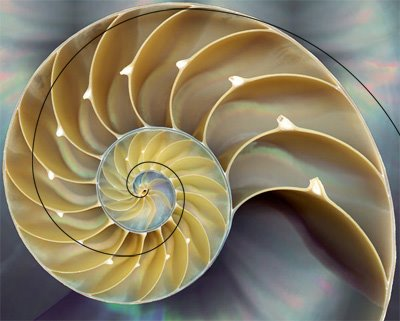
\includegraphics[width=4.3cm]{img-03/nautilus}}{chap:successions}


\vspace*{\fill}


\begin{iniaval}
 \textbf{Esbrina la regla que s'ha emprat i escriu tres nombres més de les llistes següents:}

\begin{tasks}
	\task  1, 3, 5, 7, .... , .... , ....,  $\cdots$
	\task  2, -4, 8, -16, 32, .... , .... , ....,  $\cdots$
	\task  1, 4, 9, 16, 25, 36, .... , .... , ....,  $\cdots$
\end{tasks}

\vspace{0.25cm}
\quad Inventa't una llista semblant i passa-la al teu company perquè endevini els següents termes.
\vspace{0.25cm}

 \textbf{Col·loca les paraules i forma la frase}
\vspace{0.5cm}
\begin{center}
 \textbf{REGLA \qquad\qquad LLISTA  \qquad\qquad  SUCCESSIÓ  \qquad\qquad  FIXADA  \qquad\qquad NOMBRES}
\end{center}
\vspace{0.5cm}
 \textbf{``Una ................. és una .................ordenada de .................obtinguts a partir d'una .................de formació ................''}

\vso
 
\addanswersline[cols=1]{Avaluació inicial}{0}{[Successió dels nombres senars: $1,3,5,7,9,11,13,15,\cdots$, Multiplicam per --2:\par $2,-4,8,-16,32,-64,128,-256,\cdots$, Successió dels quadrats:\par $1,4,9,16,25,36,49,64,81,\cdots$ ]}
\end{iniaval}

\vspace*{\fill}

\pagebreak
\section{ Successions}

\begin{theorybox}
 \video[ytid=MUZZ7aFAIDA]{134}{Successions}
 Una \textbf{successió} és una \textbf{llista ordenada} de nombres obtinguts a partir d'una regla de formació fixada. A cadascun dels nombres se'ls anomena \textbf{terme}. Per exemple, la llista de nombres senars 1, 3, 5, $\cdots$ té com a primer terme $a_1 = 1$, segon terme $a_2=3$, etc.
 
 Una successió es pot donar de diferents formes:
 \begin{itemize}
 	\exer Donants els seus primers termes: 1, 3, 5, 7, $\cdots$
 	\exer A partir del terme general:  $a_n = 2n-1$
 	\exer A partir d'una relació de recurrència:  $a_1 = 1$ i $a_{n+1} = a_n + 2$
 \end{itemize}
\end{theorybox}
\vspace{-0.5cm}
\begin{blueshaded}
	Una manera forma fàcil d'entendre què és una successió és agafar la llista de classe i escriure devora de cada número de llista, per exemple, el mes de naixement de l'alumne:
	
	\begin{minipage}{0.5\textwidth}
	 	\begin{tabular}{lcc}
	 	\textbf{Nom} & $\mathbf{n}$ & $\mathbf{a_n}$ \\ \hline	
	 	\emph{Amengual} & 1 $\rightarrow$ & 2 \\
	 	\emph{Bibiloni} & 2 $\rightarrow$ & 7 \\
	 	\emph{Cerdà}    & 3 $\rightarrow$ & 5 \\
	 	\emph{Deyà}    & 4 $\rightarrow$ & 11
	 \end{tabular}
	\end{minipage}
	\begin{minipage}{0.5\textwidth}	
		En la successió $a_n= 2, 7, 5, 11, \cdots$,
		
		\qquad $\mathbf{a}$ és el valor del mes 
		 
		 \qquad $\mathbf{n}$ és el número de llista.
	\end{minipage}
\end{blueshaded}


\begin{mylist}

\exer  \spen Escriu els deu primers termes de les següents successions:
\begin{tasks}(3)
	\task   $-$1, $-$2, $-$3, $-$4,{\dots}   
	\task  1, 4, 9, 16,{\dots}   
	\task  1, 3, 5, 7,{\dots}
\end{tasks}
\vso
\answers[cols=1]{[$-1,-2,-3,-4,-5,-6,-7,-8,-9,\cdots$, $1,4,9,16,25,36,49,64,81,100,\cdots$, $1,3,5,7,9,11,13,15,17,\cdots$]}

\exer \spen  Escriu el terme que ocupa el lloc 100 de cadascuna de les successions anteriors.
\vso
\answers[cols=1]{[$a_n=-n;\,\,a_{100}=-100$, $a_n=n^2;\,\,a_{100}=100^2=10000$. $a_n=2n-1,\,\,a_{100}=199$]}

\exer  Sabem que un cos que cau lliurement sobre la Terra té una velocitat que augmenta 9,8 m/s cada segon. Si en el primer segon la seva velocitat és de 15 m/s, escriu en el teu quadern la velocitat en els segons indicats en la taula. Observes alguna regla que et permeti conèixer la velocitat al cap de 20 segons? Representa gràficament aquesta funció.
\end{mylist}
\begin{center}
\renewcommand{\arraystretch}{2}
\begin{tabular}{|p{0.25\textwidth}|p{0.2\textwidth}|p{0.2\textwidth}|p{0.2\textwidth}|}\hline 
\textbf{Temps en segons} & 1 & 2 & 3 \\ \hline 
\textbf{Velocitat en m/s} & 15 &  &  \\ \hline 
\end{tabular}
\end{center}

\answers{Les velocitats passats $n$ segons són: $v_n=15+(n-1)\cdot 9.8$.\par 
Passats $n=2$ segons; $v_2=24.8$ m/s. \par Passats $n=3$ segons; $v_3=34.6$ m/s. 
\par Passats $n=20$ segons; $v_{20}=15+(20-1)\cdot 9.8=201.2$ m/s.} 
 
\pagebreak
 
\begin{resolt}[E]{
		Troba els 5 primers termes de la successió donada en forma recurrent:
		
		$a_1 = 2$
		
		$a_2 = 1$
		
		$a_n = 3 a_{n-1} + 2 a_{n-2}$
		
	}
	Ens donen el primer i segon termes i la relació per trobar els següents. El tercer terme s'obté de fer el triple del segon més el doble del primer.
	\[ a_3 = 3 \cdot 1 + 2 \cdot 2 = 7  \]
	\[ a_4 = 3 \cdot 7 + 2 \cdot 1 = 23  \]
	\[ a_5 = 3 \cdot 23 + 2 \cdot 7 = 83  \]
	\[ \cdots \]
\end{resolt}

\begin{mylist}

\exer  Escriu els quatre primers termes de les següents successions: 

 $a_n = 2 n^2+1$  \quad \quad  $b_n = \frac{4n-1}{3n}$ \quad \quad
 %%%%
 $ \begin{array}{c}
c_1\ =\ 1; \\ 
c_n\ =\ 3c_{n-1}\ +\ 5 \end{array}
$
\quad \quad
%%%%
$\begin{array}{c}
d_1=\ 2;\ \ d_2=5; \\ 
d_n\ =\ 2d_{n-1}\ +\ d_{n-2} \end{array}$
 
 \answers[cols=1]{[$a_n=3,9,19,33,\cdots$, $b_n=1,\frac{7}{6},\frac{11}{9},\frac{5}{4},\cdots$, $c_n=1,8,29,92,\cdots$, $d_n=2,5,12,29,\cdots$]}


\exer  Escriu l'expressió del terme general de les següents successions:

\begin{tasks}(2) 
	\task  $\{-1, 1, -1, 1, -1, 1, -1, 1, {\dots}\}$      
	\task  $\{0, 3, 8, 15, 24, 35,{\dots}\}$  
	\task  $\{2, 4, 6, 8, 10,{\dots}\}$       
	\task  $\left\{\frac{1}{4} ,{\rm \; }\frac{3}{5} ,\frac{5}{6} {\rm \; ,}\frac{{\rm 7}}{{\rm 7}} ,\frac{9}{8} ,...\right\}$
\end{tasks}

\answers[cols=2]{[$a_n=(-1)^{n}$, $a_n=n^2-1$, $a_n=2\cdot n$, $a_n=\frac{2\cdot n-1}{3+n}$]}
 
\exer \spen  En una successió el primer terme és 2 i els altres s'obtenen sumant 4 al terme anterior. Calcula els 6 primers termes de la successió.
\vsoo
\answers{Primers termes: $2,6,10,14,18,\cdots$.\par Terme general: $a_n=2+4\cdot(n-1)$}

\exer  Un satèl·lit artificial es va posar en òrbita a les 17:30 hores. Tarda a fer una volta completa a la seva òrbita 1:27 hores.

\begin{minipage}{0.84\textwidth}
\begin{tasks}
\task Completa en el teu quadern la taula adjunta.

	\begin{tabular}{|p{1.5in}|p{0.34in}|p{0.34in}|p{0.34in}|p{0.34in}|p{0.34in}|p{0.34in}|} \hline 
		\textbf{N${}^\circ$  d'òrbites} & \textbf{1} & \textbf{2} & \textbf{3} & \textbf{4} & \textbf{5} & \textbf{6} \\ \hline 
		\textbf{Hora en la qual l'ha completat} &  &  &  &  &  &  \\ \hline 
	\end{tabular}
%
\task Escriu una expressió general que et permeti conèixer l'hora en què ha completat la tornada enèsima.
%
\task Cerca una expressió que et permeti conèixer l'hora en funció de l'hora de l'òrbita anterior.
%
\task Cerca una expressió que et permeti conèixer l'hora en funció de la primera.
%
\task Quantes voltes completes haurà donat 20 dies més tard a les 14:00 hores?
\end{tasks}
\end{minipage}
\begin{minipage}{0.16\textwidth}
	\centering
	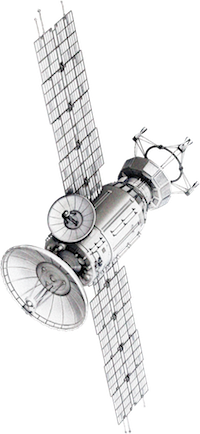
\includegraphics[width=0.8\textwidth]{img-03/satellite}
\end{minipage}

\answers[cols=1]{[Taula: $18:57$; $20:24$; $21:51$; $23:18$; $00:45$; $02:12$, 
		  Expressió general: $t_n = 17:30 + n\cdot 1:27$ on $n$ són el número de voltes completades,
		  Recurrent:  $t_1=18:57$; $t_n=1:27+t_{n-1}$,
		  $t_n = 18:57 + (n-1)\cdot 1:27$ on $n$ són el número de voltes completades,
		  Dividim l'interval 476.5 hores entre el temps d'una volta 1.45 hores: Ha completat 328 voltes a les 13:06.]}

\end{mylist}


\vspace{4cm}

\section{Progressions aritmètiques}

\begin{theorybox}

 \video[ytid=E\_BOmk0n6Eo]{132}{Progressions aritmètiques}

                 Les progressions aritmètiques són successions en què la diferència entre dos termes consecutius (anomenada \textbf{diferència d}) es manté constant. 

      \textbf{Terme General: }  $a_n=\ a_1+d\textrm{·}(n-1)$

 \textbf{Suma dels primers N termes:}  $S_N=N\textrm{·}\frac{(a_1+a_N)}{2}$

\end{theorybox}

 
\begin{mylist}

\exer \spen Assenyala raonadament si la següent successió és una progressió aritmètica: $\{1, 10, 100, 1000, 10000, {\dots}\}$.
\vso
\answers{No és una progressió aritmètica perquè la diferència entre dos termes consecutius no és constant.}

\exer  Calcula els tres primers termes d'una progressió aritmètica sabent que el primer és 1 i la diferència és $-2$.
\vso
\answers{$1,-1,-3,-5,-7,\cdots$}

\begin{resolt}[E]{
		 Calcula el terme 100 \linebreak d'una progressió aritmètica amb diferència 7 i $a_{15} = 165$. 
	}
	Escrivim el terme general de la progressió 
	
	\[a_{15} = 165 = a_1 + 7 \cdot (15 -1)\]
	
	 D'aquí aïllam el valor del primer terme $a_1 = 67$. 
	\vspace{0.25cm}
	
	Ara cercam el terme 100: $a_{100} = 67  + 7 \cdot (100 -1) =760$.
\end{resolt}
 
\exer  Calcula el primer terme d'una progressió aritmètica amb diferència 2 i $a_{30} = 60$. 
\answers{$a_{30}=a_1+2\cdot(30-1)$  $\rightarrow$ $60=a_1+58$, aïllam $a_1=60-58=2$}

\exer  Donada una progressió aritmètica dos dels termes de la qual són: $a_{3} = 4$ i $a_{10} = 18$.

\begin{tasks}(2)
 \task Calcula la seva diferència.
 \task Calcula el seu terme general.
\end{tasks}
\answers[cols=1]{[La diferència és $d=(18-4)/(10-3)=2$, Necessitam el primer terme: $a_1=0$ El terme general és $a_n=0+2\cdot (n-1)$. Efectivament comprovam que $a_{10}=18$]}


\exer  Quin és el terme general d'una progressió aritmètica amb $a_{22} = 45$ i $d = 3$?
\answers{El primer terme és $45=a_1+3\cdot 21$ $\rightarrow$ $a_1 =-18$. El terme general $a_n=-18+3(n-1)$}

\exer  Els costats d'un pentàgon estan en progressió aritmètica de diferència 5. Sabent a més que el seu perímetre és 65, calcula el valor dels costats.
\answers{Recorda que $S=N\cdot \bar x$ on $\bar x$ és el valor mitjà de la progressió aritmètica. $65=5\cdot \bar x$ $\rightarrow$ $x=13$ és el valor d'enmig i els altres les trobam sumant o restant 5: 3; 8; 13; 18 i 23.}

\exer  Calcula els 5 primers termes d'una progressió aritmètica de primer terme 2 i de diferència 3. Representa'ls gràficament. Observa que la seva representació gràfica és un conjunt de punts aïllats que estan sobre una recta.
\answers{2, 5, 8, 11 i 14.}

\exer  Calcula l'expressió general de les progressions aritmètiques:

\begin{tasks}
	\task De diferència $d = 2.5$ i de primer terme 2.
	\task De diferència $d = -2$ i de primer terme 0.
	\task De diferència $d = 1/3$ i de segon terme 5.
	\task  De diferència $d = 4$ i de cinquè terme 1.
\end{tasks}
 \answers[cols=1]{[$a_n=2+2.5(n-1)$, $a_n=0-2(n-1)$, $a_n=\frac{14}{3}+\frac{1}{3}(n-1)$, $a_n=-15+4(n-1)$]}


\exer Quants múltiples de 7 estan compresos entre el 4 i el 893?
\answers{127}

\exer[1]  Suma els 10 primers termes de la progressió aritmètica: $\{-5, 4, 13, 22, 31, 40, {\dots}\}$
\answers{Sumen 355}

\exer[1]  Troba la suma dels 50 primers múltiples de 3.
\answers{Sumen 3825}
	
\begin{comment}
\exer  En una successió aritmètica d'un nombre imparell de termes el central val 12, quant valdrà la suma del primer terme més el darrer terme?

\end{comment}

\exer[1]  L'amo d'un pou contracta a un saurí per conèixer la profunditat a la qual es troba l'aigua i aquest dictamina que a 5 m hi ha aigua en abundància. Demana un pressupost a un contractista, que li diu que el primer metre li costarà 50 euros i per cada mig metre més 6 euros més que pel mig metre anterior. Quant li costarà el pou si es compleixen les prediccions? 
\answers{98 \euro{}}
	
\exer  Antoni s'ha comprat un mòbil, però no pot pagar-ho al comptat. Paga 60 euros cada setmana, però el venedor li puja 5 euros cada setmana en concepte de pagament ajornat. Aconsegueix pagar-ho en 10 setmanes. Quant li va costar? Quant va pagar de més? Quin percentatge suposa aquest recàrrec sobre el preu de venda?
\answers{825, 225, 37.5\%}
	
\exer  Un nedador s'entrena en una piscina de 50 m i vol controlar les pèrdues de velocitat per cansament. Cronometra en cinc dies consecutius els temps que triga a fer 2, 5, 8, 11, 14 llargs. Es demana:

\begin{tasks}
	\task El terme general de la successió $a_n$ que dóna els metres recorreguts en el dia $n$.
	\task  Quants metres haurà nedat en aquests cronometratges?
\end{tasks} 
\answers{[$a_n =100 + 150 (n – 1)$, 100; 250; 400; 550 i 700 metres]}
  

\end{mylist}


%%%%%%%%%%%%%%%%%%%%%%%%%%%%%%%%%%%%%%%%%%%%%%%%%%%%%%%%%%%%%%%%%%%%%%%%%%%%%%%%%%%%%%%%%%%%%%%%%%%%%%%%%%%%%%%%

\section{Progressions geomètriques}

\begin{theorybox}

 \video[ytid=U6kGF1PQEr4]{133}{Progressions geomètriques}

  Les progressions geomètriques són successions en les quals el quocient de dos termes consecutius (anomenat \textbf{raó $r$}) es manté constant. 

  \textbf{Terme general: }  $a_n=\ a_1{\textrm{·}r}^{n-1}$

 \textbf{     Suma dels primers N termes:}  $S_N=\frac{a_1{\textrm{·}(r}^N-1)}{r-1}\ $

 \textbf{     Suma dels infinits termes (si 0$\boldsymbol{<}$r$\boldsymbol{<}$1):} $S_{tots}=\frac{a_1}{1-r}$
\end{theorybox}


\begin{mylist}

\exer \spen Esbrina la raó d'una progressió geomètrica el segon terme de la qual és 27 i el tercer és 3.
\vso
\answers{$r=\frac{3}{27}=\frac{1}{9}$}

\exer \spen  El quart terme d'una progressió geomètrica és $\frac{1}{9}$ i la raó 3. Troba el primer terme.
\vso
\answers{$a_1=\frac{1}{243}$}

\exer  Troba el sisè terme de la següent progressió geomètrica: $\{$$\sqrt{2} $, 2, 2$\sqrt{2} $, 4,{\dots}$\}$
\answers{La raó és $\sqrt{2}$. Els següents termes són: $\{\sqrt{2},2,2\sqrt{2},4,4\sqrt{2},8,8\sqrt{2},16,{\cdots}\}$ }

\end{mylist}

\begin{resolt}[E]{
		D'una progressió geomètrica sabem que $a_1=625$ i $a_4=320$. Troba la raó i el terme cinquè.
	}
	El primer és trobar la raó:
	
	\[ a_4 = a_1 \cdot r^{4-1}  \, \rightarrow \, 320 = 625 \cdot r^3 \, \rightarrow \,  r^3 = 320/625=0,512 \,   \]
	
	La raó és $ r=\sqrt[3]{0,512}=0,8$. Finalment trobam el terme cinquè:
	\[ a_5 = a_1 \cdot r^{5-1}  \, \rightarrow \, a_5 = 625 \cdot (0,8)^4 = 256  \]
	
\end{resolt}

\begin{mylist}
\exer[1]  Donada una progressió geomètrica dos dels termes de la qual són: $a_{3} = -8$ i $a_{5} = -32$. 
\begin{tasks}(2)
	\task   Calcula la seva raó.   \task Calcula el seu terme general.
\end{tasks}
\answers{Raó $-2$, terme general $a_n=(-2)^n$}

\begin{comment}
\exer  Certa classe d'alga, anomenada \textit{clorella}, es reprodueix duplicant la seva quantitat cada dues hores i mitja. Al cap d'altres dues hores i mitja torna a duplicar la seva quantitat, i així successivament. Si es té en el moment inicial un quilo, al cap de dues hores i mitja hi ha dos quilos.


 a) Fes una taula de valors en la qual indiquis per a cada període de reproducció el nombre de quilos de \textit{clorella}.

 b) Indica el terme general.

 c) Al cap de 4 dies, han transcorregut 40 períodes, consideres possible aquest creixement? 
\end{comment}

\exer  Calcula el producte dels 15 primers termes de la progressió: 3, 6, 12, 24, $\cdots$

\answers{Terme general $a_n=3\cdot 2^{n-1}$.\par Terme 15è és $a_{15}=3\cdot 2^{14}=49152$.\par Producte $P_{15}=\sqrt{(3\cdot 49152)^{15}}=5.82\cdot 10^{38}$}

\exer  Un agricultor en la seva granja té 59049 litres d'aigua per donar de beure als animals. Un dia va utilitzar la meitat del contingut, al següent la meitat del que li quedava i així successivament cada dia. Quants litres d'aigua va utilitzar fins al sisè dia?
\answers{$a_1=59049:2=29524.5$. Progressió de raó 1/2 $a_n=29524.5 \cdot (1/2)^{n-1}$.\par El sisè dia consumeix 922.64.\par En total en aquests 6 dies $S_6= \frac{29524.5 \cdot(0.5^6-1)}{0.5-1}=58126.36$ litres. És a dir li queden 922.64 litres.}

\exer[1]  Troba la suma els 15 primers termes d'una progressió geomètrica en la qual $a_{1} = 5$  i $r = \ofrac{1}{2}$.
\answers{Els 15 primers termes sumen $\dfrac{163835}{16384}$}

\exer[1]  Calcula la suma dels infinits termes de la successió: 6, 3, $\frac{3}{2}$, $\frac{3}{4}$, {\dots}
\answers{Els infinits termes sumen 12}

\exer  Tenim a la mà un quadrat d'àrea 1. Tallem les quatre cantonades pels punts mitjans dels costats. El nou quadrat, quina àrea té? Deixem les retallades damunt de la taula. Quina àrea de retallades hi ha sobre la taula? Amb el nou quadrat que tenim a la mà efectuem la mateixa operació de tallar les quatre cantonades i deixar-les sobre la taula, i així successivament. Quina àrea tenen els successius quadrats que tinc a la mà? I les retallades que queden sobre la taula? Troba la suma de les infinites àrees de retallades així obtingudes.
\begin{center}
	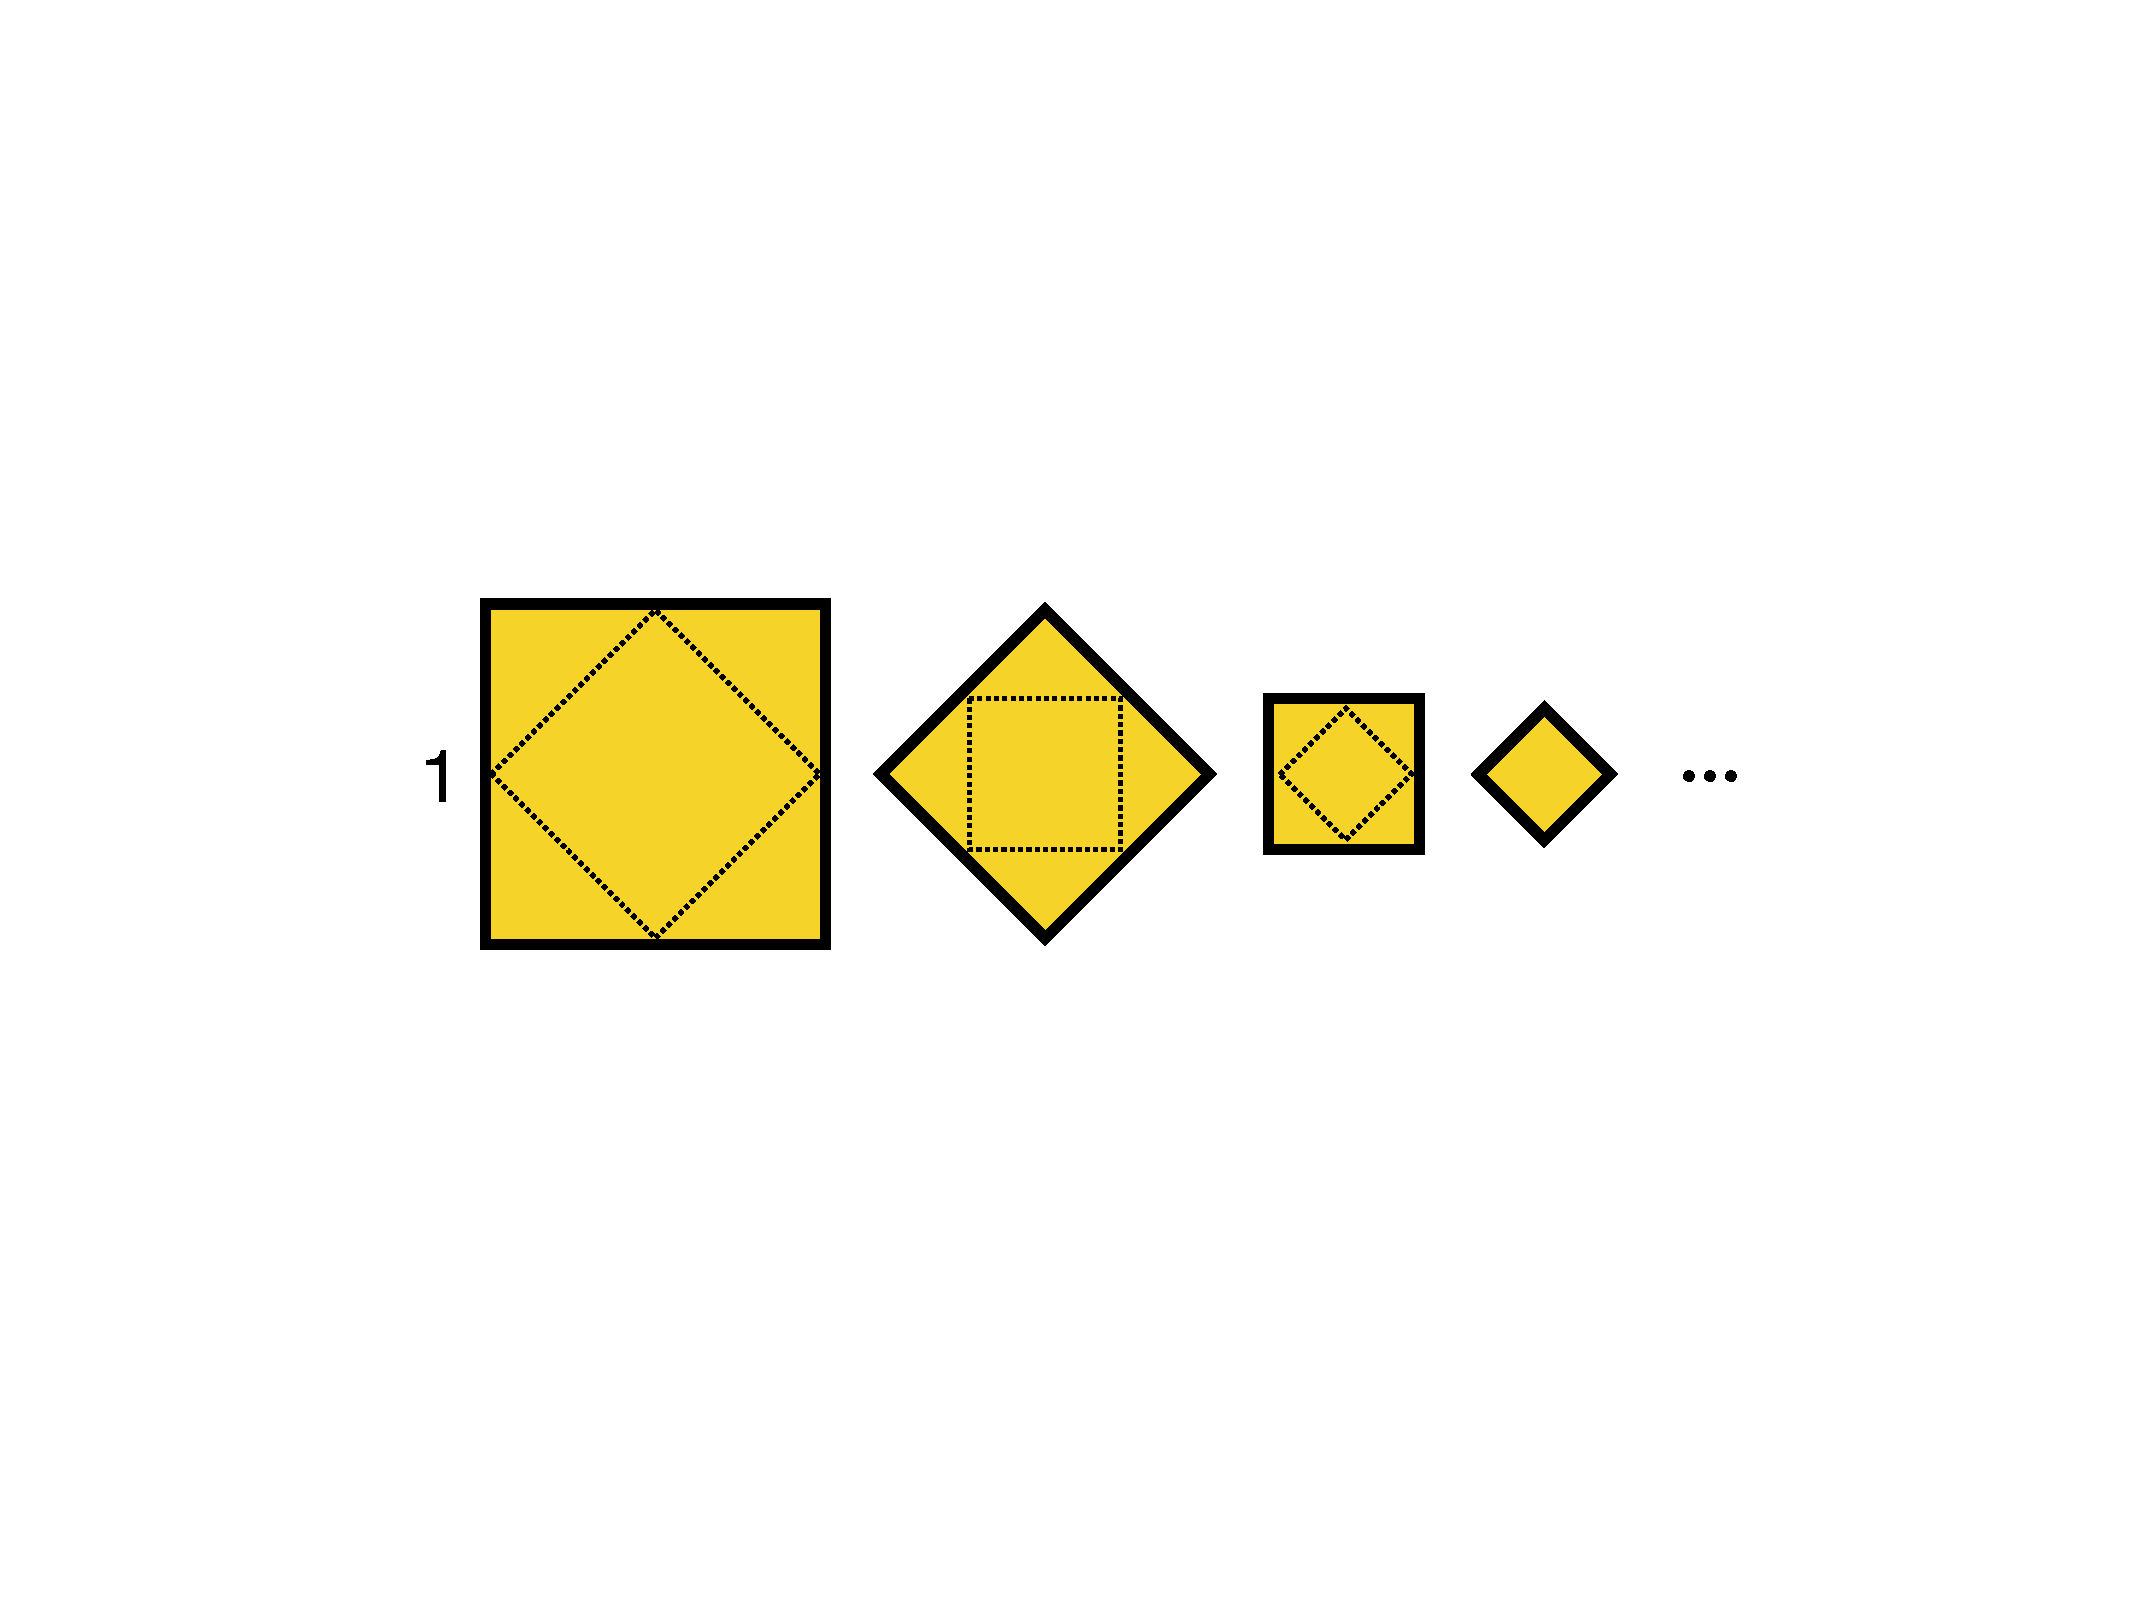
\includegraphics[height=2cm]{img-03/quadrats}
\end{center}
\answers{La successió d'àrees dels quadrats és $1, 1/2, 1/4, 1/8, \cdots$.\par La successió de les retallades és $0, 1/2, 3/4, 7/8, 15/16, \cdots$. \par Veim que la suma de les àrees retallades s'acosta a 1.\par $S_\infy=\frac{0.5}{1-0.5}=1$ }

\begin{comment}
\exer  De nou tenim un quadrat d'àrea 1 a la mà, i ho tallem per les línies de punts com indica la figura. El tros major ho deixem sobre la taula i ens quedem a la mà amb el quadrat, al que tornem a tallar de la mateixa forma. I així successivament. Quina àrea tenen els successius quadrats que tinc a la mà? Creixen o disminueixen? Escriu el terme general de la successió d'àrees que tenim a la mà. I les retallades que queden sobre la taula? Creix l'àrea o disminueix? Anem sumant àrees, calcula la suma d'aquestes àrees si haguéssim fet infinits talls.
\end{comment}

\exer  Calcula la fracció generatriu del número $4,\hat{5}$. Ajuda $4,\hat{5}=4+5\textrm{·}{10}^{-1}+5\textrm{·}{10}^{-2}+\textrm{·}\textrm{·}\textrm{·}$
\answers{$4+5(0.1+0.01+0.001+...)=4+5\frac{0.1}{1-0.1}=4+\frac{5}{9}=\frac{41}{9}$}

\exer  Un empresari acudeix a una entitat financera per informar-se sobre com invertir els 6000 \euro{} de beneficis que ha tingut en un mes. Li plantegen dues opcions.
\begin{tasks}
\task  Mantenir aquest capital durant 5 anys al 3,5 \% anual, 
\task  Rebre el 5 \% del capital durant els dos primers anys i el 3 \% els tres anys restants. 
\end{tasks}
Quina opció li interessa més?
\end{mylist}
\answers{La millor opció és la b) $2\frac{5}{100}\cdot 6000+3\frac{3}{100}\cdot 6000=1140$ euros,\par comparat amb $5\frac{3.5}{100}\cdot 6000= 1050$ euros d'interès.}
\newpage




\begin{activitats}
	
\begin{mylist}
\exer  Calcula el terme 100 d'una progressió aritmètica el primer terme de la qual és 4 i la diferència és 5. 
\answers{$a_{100}=4+5\cdot (100-1)=499$}
 
\exer  El desè terme d'una progressió aritmètica és 45 i la diferència és 4. Troba el primer terme. 
 \answers{$45=a_1+4\cdot (10-1)$ $\,\rightarrow\,$ $a_1=9$}
 
\exer  Sabent que el primer terme d'una progressió aritmètica és 4, la diferència 7 i el terme 88, troba $n$. 
\answers{$88=4+7\cdot(n-1)$ $\,\rightarrow\,$  $n=\frac{88-4}{7}+1=13$}

\exer  Troba el primer terme d'una progressió aritmètica i la diferència, sabent que $a_{3} = 24$ i $a_{10} = 66$. 
\answers{$d=\frac{66-24}{10-3}=6$ $\,\rightarrow\,$  $a_1=24-2\cdot 6=12$}

\exer  El terme sisè d'una progressió aritmètica és 4 i la diferència 1/2. Troba el terme 20. 
\answers{$a_1=1.5$, $a_n=1.5+0.5 (n-1)$. El terme 20 és $a_{20}=1.5+ 0.5 \cdot 19 = 11$}

\exer \hot Calcula els costats d'un triangle rectangle sabent que les seves mesures, expressades en metres, estan en progressió aritmètica de diferència 3. 
\answers{Els costats són  $x-3$, $x$ i $x+3$. Aplicam Pitàgores: $(x+3)^2=(x-3)^2+x^2$, efectuam les identitats notable $x^2-12x=0$, trobam $x=12$. El triangle té costats 9, 12 i 15}

\exer  Calcula la suma dels múltiples de 59 compresos entre 1000 i 2000. 
\answers{Sumen 25075}
\begin{comment}
\exer  El producte de tres termes consecutius d'una progressió aritmètica és 80 i la diferència és 3. Troba aquests termes. 
\end{comment}

\exer  Quants termes cal sumar de la progressió aritmètica 2, 8, 14,... per obtenir com a resultat 1064? 
\answers{S'han de sumar 19 termes}

\exer \hot La suma de \textit{n} nombres naturals consecutius presos a partir d'11 és 1715. Quants termes hem sumat? 
\answers{$\frac{11+11+(n-1)}{2}\cdot n = 1715$. Trobam l'equació $n^2+21n-3430=0$. Hem sumat 49 números}

\exer  Sabent que el cinquè terme d'una progressió aritmètica és 18 i la diferència és 2, troba la suma dels nou primers termes de la successió. 
\answers{Els 9 primers termes sumen 162}

\begin{comment}
\exer  La suma de tres nombres en progressió aritmètica és 33 i el seu producte 1287. Troba aquests nombres. 

\exer  Tres nombres en progressió aritmètica tenen per producte 16640; el més petit val 20. Troba els altres dos. 


\exer  El producte de cinc nombres en progressió aritmètica és 12320 i la seva suma 40. Troba aquests nombres sabent que són enters. 

\exer  Calcula tres nombres sabent que estan en progressió aritmètica, que la seva suma és 18 i que la suma del primer i del segon és igual al tercer disminuït en dues unitats. 

\exer  La suma dels onze primers termes d'una progressió aritmètica és 176 i la diferència dels extrems és 30. Troba els termes de la progressió. 

\exer  La diferència d'una progressió aritmètica és 4. El producte dels quatre primers termes és 585. Troba els termes. 

\exer  En una progressió aritmètica el onzè terme excedeix en 2 unitats al vuitè, i el primer i el novè sumen 6. Calcula la diferència i els termes esmentats. 
\end{comment}
\exer  Sabent que les mesures dels tres angles d'un triangle estan en progressió aritmètica i que un d'ells mesura 100${}^\circ$ , calcula els altres dos. 
\answers{$a_1=100$, $a_2=100-d$, $a_3=100-2d$. La diferència és $40$ i els angles $100^\circ$, $60^\circ$ i $20^\circ$.}

\exer  Troba les dimensions d'un ortòedre sabent que estan en progressió aritmètica, que sumen 78 m i que el volum de l'ortòedre és de 15470 m${}^{3}$. 
\answers{17, 26 i 35}
\begin{comment}
\exer  Els sis angles d'un hexàgon estan en progressió aritmètica. La diferència entre el major i el menor és 60${}^\circ$ . Calcula el valor de cada angle. 
\end{comment}

\exer  Les longituds dels tres costats d'un triangle rectangle estan en progressió aritmètica i sumen 36 metres. Quant mesura cada costat? 
\answers{9, 12 i 15.}

\exer  Un coronel ordena a 5050 soldats que formin un triangle per a una exhibició, de manera que la primera fila tingui un soldat, la segona dues, la tercera tres, etc. Quantes files han d'haver-hi? 
\answers{100 files, perquè $1+2+3+4+\cdots+100=5050$}

\exer  Pel lloguer d'una casa s'acorda pagar 800 euros al mes durant el primer any, i cada any s'augmentarà el lloguer en 50 euros mensuals. Quant es pagarà mensualment al cap de 12 anys? 
\answers{$a_{12}=800+50 (12-1)=1350$ \euro{}.}

\exer  Les edats de quatre germans formen una progressió aritmètica, i la seva suma és 32 anys. El major té 6 anys més que el menor. Troba les edats dels quatre germans. 
\answers{$x$, $x+d$, $x+2d$, $x+3d$. Sabem que $4x+6d=32$ i que $x+3d-x=6$. Llavors $d=2$ i $x=5$. Les edats són $5, 7, 9, 11$ anys.}

\exer  Un esquiador comença la pretemporada d'esquí fent peses en un gimnàs durant una hora. Decideix incrementar l'entrenament 10 minuts cada dia. Quant temps haurà d'entrenar al cap de 15 dies? Quant temps en total haurà dedicat a l'entrenament al llarg de tot un mes de 30 dies? 
\answers{[$a_{15} = 200$ minuts, 6150 minuts en un mes.]}

\exer  En una sala de cinema, la primera fila de butaques dista de la pantalla 86 dm, i la sisena, 134 dm. En quina fila estarà una persona si la seva distància a la pantalla és de 230 dm? 
\answers{$d_n=86+9.6(n-1)$. $230=86+9.6(n-1)$ i aïllam $n$. La fila és la 16}

\exer  Calcula el terme onzè d'una progressió geomètrica el primer terme de la qual és igual a 1 i la raó és 2. 
\answers{$a_{11}=1\cdot 2^{11-1}=2^{10}=1024$}

\exer  En una progressió geomètrica de primer terme 7 i raó 2, un cert terme és 28672. Quin lloc ocupa aquest terme? 
\answers{$28672=7\cdot 2^{n-1}$. Dividim entre 7;\, $4096=2^{n-1}$. Trobam que $n=13$.}

\exer  Sabent que el setè terme d'una progressió geomètrica és 1 i la raó 1/2, troba el primer terme. 
\answers{$1=a_1 \cdot (0.5)^{7-1}$ aïllam $a_1 = \frac{1}{0.5^6}=64$}

\begin{comment}
\exer  El volum d'un ortòedre és de 3375 cm${}^{3}$. Troba la longitud de les seves arestes, sabent que estan en progressió geomètrica i que l'aresta intermèdia mesura 10 cm més que la menor. 


\exer  Troba el producte dels vuit primers termes de la progressió 3, 6, 12, 24,... 
\end{comment}

\exer  Troba la suma dels deu primers termes de la progressió geomètrica 3, 6, 12, 24,... 
\answers{$S_{10}=\frac{3 (2^{10}-1)}{2-1}=3069$}

\exer  Troba la suma dels termes de la progressió il·limitada: 8, 4, 2, 1,... 
\answers{$S_{tots}=\frac{8}{1-0.5}=16$}

\begin{comment}
\exer  Troba tres nombres en progressió geomètrica sabent que la seva suma és 26 i el seu producte 216. 
\end{comment}

\exer  La suma dels set primers termes d'una progressió geomètrica de raó 3 és 7651. Troba els termes primer i setè. 
\answers{$7651=a_1\frac{3^7-1}{3-1}$. Aïllam $a_1=\dfrac{7651}{1093}=7$. El terme 7è $a_7=7\cdot 3^6=5103$.}

\exer \hot  Troba els quatre primers termes d'una progressió geomètrica, sabent que el segon és 20 i la suma dels quatre primers és 425. 
\answers{$r \cdot a_1=20$ i $425=a_1\frac{r^4-1}{r-1}$. Té solució $a_1=5$ i $r=4$ Els termes són: 5, 20, 80 i 320.}

\exer  Les dimensions d'un ortòedre estan en progressió geomètrica. Calcula aquestes dimensions sabent que el seu perímetre és 420 m i el seu volum 8000 m${}^{3}$.
\answers{Les dimensions són 5, 20 i 80}
\begin{comment}
\exer  Divideix el número 221 en tres parts enteres que formen una progressió geomètrica tal que el tercer terme sobrepassa al primer en 136. 
\end{comment}

\exer  La suma de tres nombres en progressió geomètrica és 248 i la diferència entre els extrems 192. Troba aquests nombres. 
\answers{$x+rx+r^2x=248$ i $x(r^2-1)=192$. Els nombres són: 8, 40 i 200} 

\exer  Troba quatre nombres en progressió geomètrica sabent que la suma dels dos primers és 28 i la suma dels dos últims 175. 
 \answers{8, 20, 50 i 125}
 
\exer  Una progressió geomètrica té cinc termes, la raó és igual a la quarta part del primer terme i la suma dels dos primers termes és 24. Troba els cinc termes. 
\answers{$r=x/4$ i $x+rx=24$. Els termes són 8, 16, 32, 64 i 128}

\exer  A una corda de 700 m de longitud se li fan dos talls, de manera que un dels trossos extrems té una longitud de 100 m. Sabent que les longituds dels trossos estan en progressió geomètrica, determina la longitud de cada tros. 
\answers{Els trossos de corda són 100, 200 i 400.}

\exer  Troba la fracció generatriu del nombre decimal 0,737373..., com suma dels termes d'una progressió geomètrica il·limitada.  Ajuda:  $0,737373=73\textrm{·}{100}^{-1}+\ 73\textrm{·}{100}^{-2}+\cdots$
\answers{73/99.}

\exer  Es té una bota de vi que conté 1024 litres. L'1 d'octubre es va buidar la meitat del contingut; l'endemà es va tornar a buidar la meitat del que quedava, i així successivament tots els dies. Quina quantitat de vi es va treure el dia 10 d'octubre? 
\answers{1 litre}

\exer  Donat un quadrat d'1 m de costat, unim dos a dos els punts mitjans dels seus costats; obtenim un nou quadrat, en el qual tornem a efectuar la mateixa operació, i així successivament. Troba la suma de les infinites àrees així obtingudes.
\answers{Les infinites àrees sumen 2 m$^2$} 

\exer  Tres nombres que la seva suma és 36 estan en progressió aritmètica. Troba aquests nombres sabent que si se'ls suma 1, 4 i 43, respectivament, els resultats formen una progressió geomètrica. 
\answers{[PG: 4; 16 i 64, PA: 3; 12 i 21]}

\exer[1] 
\textit{Triangle de Sierpinski}: Anem a construir un fractal. Es parteix d'un triangle equilàter. S'uneixen els punts mitjans dels costats i es formen quatre triangles. S'elimina el triangle central. En cadascun dels altres tres triangles es repeteix el procés. I així successivament. A la figura formada per iteració infinita la hi denomina Triangle de Sierpinski, i és un fractal.
 	\begin{center}
	\includegraphics*[width=0.38\textwidth]{img-03/sierpinski}
\end{center} 

 Imagina que el primer triangle té àrea $A$. Quan apliquem la primera iteració, l'àrea és $(3/4)A$. I en la segona? Escriu la successió de les àrees. És creixent o decreixent? Imagina ara que la longitud de cada costat del triangle inicial és $L$. Escriu la successió de perímetres. És creixent o decreixent? 
 \answers{[$A_n = A \cdot (3/4)^{n-1}$ decreixent, $P_n = 3L \cdot (3/2)^{n-1}$ creixent]}

\end{mylist}
 
\end{activitats}

\pagebreak
\begin{autoaval}{32}

\begin{mylist}

\exer[2]  Quina és la raó de la següent progressió a${}_{ n}$ = 5$\cdot$3\textit{${}^{n}$}${}^{-}$${}^{1}$?
\answers{La raó és 3}

\exer[2]  En la successió $7, 11, 15, 19, 23, \cdots$, quin lloc ocupa el terme 335?
\answers{Posició $n=83$}

\exer[2]  Què val la suma dels deu primers termes de la progressió aritmètica: 7, 13, 19, 25, 31,{\dots}?
 \answers{Sumen 340}
 
\exer[2]  Donada la successió $5, 15, 45, 135, 405, 1215, \cdots$, digues si és una progressió i calcula la seva diferència o raó.
\answers{És una progressió geomètrica. La raó és 3.}

\exer[2]  Calcula el terme general de la successió: $2, 10, 50, 250, 1250, \cdots$.
\answers{Progressió geomètrica $a_{n} = 2 \cdot 5^{n-1}$  }

\exer[2] Quant sumen les potències de 2 compreses entre 2${}^{1}$ i 2${}^{10}$?
\answers{Sumem 2046}
 
\exer[2]  Calcula el terme general de la progressió aritmètica el primer terme de la qual és 1 i la seva diferència 2.
\answers{ $a_{ n} = 2n + 1$ }

\exer[2]  Quin és el valor de la suma: 1 + 3 + 5 + 7 + ... + 999?
\answers{250.000}
 
\exer[2]  Maria està preparant l'examen de selectivitat. Per no deixar tota la matèria per al final ha decidit estudiar cada dia el doble de pàgines que el dia anterior. Si el primer dia va estudiar tres pàgines, quantes haurà estudiat al cap de 7 dies? Quantes pàgines haurà estudiat en total?
\answers{192 pàgines dia 7; 381 pàgines en total}
 
\exer[2]  A n'en Bernat li han tocat 6000 \euro{} en la loteria i decideix dipositar-los al banc a un tipus d'interès compost del 4 \%. Quants diners tindrà al cap de 5 anys?
\answers{$6000\cdot 1,04^5 = 7299,92$ \euro{}}

\end{mylist}

\end{autoaval}

\vsoo

\begin{blueshaded}
	
	La successió de \textbf{Fibonacci} comença amb dos uns i després cada terme s'obté de sumar el dos anteriors. Aquests són els primers termes:
	$
	 1, 1, 2, 3, 5, 8, 13, 21, 34, 55, 89, \cdots
	$
	
	Aquesta successió apareix en molts de casos en la naturalesa, especialment en estructures espirals com ara els caragols, el nombre de pètals de les margalides, els girasols, les pinyes, les galàxies, etc.
	
	\vspace{0.25cm}
	
	\begin{center}
		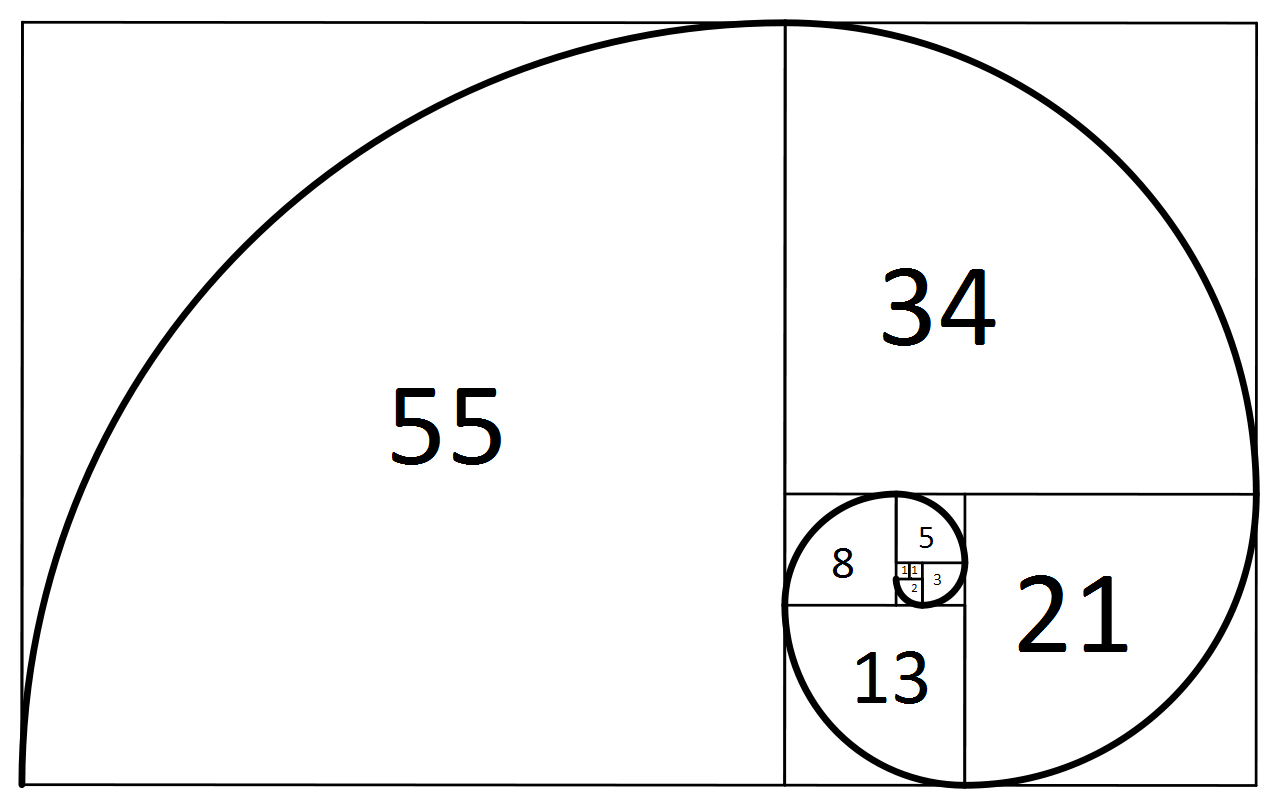
\includegraphics[height=3cm]{img-03/espiral.png}
		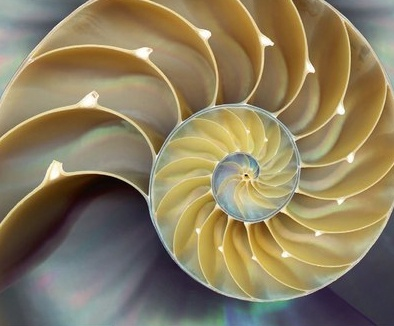
\includegraphics[height=3cm]{img-03/nautilus2.jpg}
	\end{center}

Cerca més informació sobre aquesta successió i  la seva relació amb el nombre auri.
	
	\begin{comment}
	Aquesta successió té una propietat curiosa. Si dividim dos termes consecutius trobam la successió:
	
	\[1, 2, 1.5, 1.6, 1.625, 1.6154, 1.619, 1.617, \cdots\]
	
	Resulta que aquesta successió s'acosta a un nombre que és tan important que se li va donar un nom (\textbf{el nombre auri}) $\Phi = \frac{1+\sqrt{5}}{2} = 1.618034 \cdots$
	\end{comment}
\end{blueshaded}

\newpage
\resum 

\begin{longtable}{|p{0.5\textwidth}|p{0.4\textwidth}|} \hline 
 \rowcolor{lightgray} \multicolumn{2}{|c|}{\textbf{ PROGRESSIÓ ARITMÈTICA}} \\ \hline
 És una successió de nombres reals en la qual la diferència entre dos termes consecutius de la successió és constant. Aquesta constant s'anomena \textbf{diferència} de la progressió i se sol denotar amb la lletra \textit{d}. & 2, 5, 8, 11, 14, 17, {\dots} \\ \hline 
 \rowcolor{lightgray} \multicolumn{2}{|p{0.5\textwidth}|}{\textbf{Terme general}} \\ \hline
\textit{a}${}_{ n}$ = \textit{a${}_{ }$}${}_{1}$ + \textit{d}·(\textit{n $-$ 1}) essent \textit{a}${}_{ 1}$ el primer terme & \[a_n = 2 + 3n \] \\ \hline 
\rowcolor{lightgray} \multicolumn{2}{|p{0.5\textwidth}|}{\textbf{Suma dels $n$ primers termes}} \\ \hline
 \[S_{n} =\frac{n\cdot (a_{1} +a_{n} )}{2} \] & \[S_{8} =\frac{8\cdot (2+(2+3\cdot 8))}{2}  =\] \[ = 4 \cdot (4 + 24) = 4 \cdot 28 = 112 \] \\ \hline \hline 
 \rowcolor{lightgray} \multicolumn{2}{|c|}{\textbf{PROGRESSIÓ GEOMÈTRICA}} \\ \hline
  És una successió de nombres reals en la qual el quocient entre cada terme i l'anterior és constant. A aquesta constant es denomina \textbf{raó} de la progressió i se sol denotar amb la lletra \textit{r}.\newline És a dir, $\frac{a_{i+1} }{a_{i} } =r$ sent \textit{i} un nombre natural. & \[ 3, 6, 12, 24, {\dots} \] \newline \[ 1, 1/2, 1/4, 1/8{\dots}\] \\ \hline 
  \rowcolor{lightgray} \multicolumn{2}{|p{0.5\textwidth}|}{\textbf{Terme general}} \\ \hline
 \[ a_n = a_1 \cdot r^{n-1}\] essent \textit{a${}_{ }$${}_{1}$} el primer terme de la successió & \[ a_n= 3 \cdot 2^{n-1} \]
 
 \[a_n = 1 \cdot (1/2)^{n} \] \\ \hline 
 \rowcolor{lightgray} \multicolumn{2}{|p{0.5\textwidth}|}{\textbf{Suma dels termes  }} \\ \hline
- Per a un \underbar{nombre $n$} de termes: \newline \[ S_n =\frac{r\cdot a_{n} -a_{1} }{r-1}  = \frac{a_{1} (r^{n} -1)}{r-1} \] \newline - Per a  $r<1$, i una \underbar{quantitat il·limitada} de termes:\[ S_{tots}=\frac{a_{1} }{1-r} \] & \[S_{8} = \frac{3(2^{8} -1)}{2-1}  = 3(256 - 1) =   765\] \newline \[S_{tots}=\frac{1}{1-\frac{1}{2} } = 2 \] \\ \hline 
\rowcolor{lightgray} \multicolumn{2}{|p{0.5\textwidth}|}{\textbf{Producte dels $n$ primers termes}} \\ \hline
 \textit{P${}_{n}$} = $\pm \sqrt{\left(a_{1} \cdot a_{n} \right)^{n} } $ = $\pm a_{1} \cdot r^{\ofrac{n-1}{2} } $  & \textit{P}${}_{9}$ = + $\sqrt{(3\cdot (3\cdot 2^{8} ))^{9} } $=(3 $\cdot$ 2${}^{4}$)${}^{9}$\newline  \\ \hline 
\end{longtable}


\begin{extrapage}
	
\setcounter{myenumi}{0}
\heading{FITXA 1: EXERCICIS DE SUCCESSIONS}
\vso

\begin{mylist}
	
	\item Escriu els tres primers termes de les successions
	\begin{tasks}(2)
		\task $a_n = (n-1)^3$
		\task $b_n = n + \frac{3}{n+1}$
		\task $c_n = 3 + 5(n-1)$
		\task $d_n = 3 \cdot \left( \frac{1}{2} \right)^n$
		\task $e_n = (n-1)(n-2)$
		\task $f_n = n^2 - n$
	\end{tasks}
	
	\item Calcula el terme que ocupa el lloc desè de les successions següents:
	\begin{tasks}(3)
		\task $a_n = 3n-1$
		\task $b_n = \frac{n^2+1}{2}$
		\task $c_n = (-1)^n + \frac{1}{n}$
		\task $d_n=\frac{1}{2}+\frac{(-1)^{n+1}}{10}$
		\task $e_n = n (n-1)$
		\task $f_n = \frac{n}{3} + \frac{3}{n}$
	\end{tasks}
	
	\item Forma una successió recurrent amb aquestes dades. Escriure-ne només els 6 primers termes.
	
	\qquad $j_1=2$  \qquad $j_2=3$  \qquad $j_n=j_{n-1} - j_{n-2}$  
 	
	\item Escriu els quatre primers termes de la successió següent: $a_1=\frac{1}{3}$ i $a_n = 2 a_{n-1}+3$.
	
	\item Troba el terme general de cada una de les successions. Calcula el terme 100è.
	\begin{tasks}(2)
		\task 12, 14, 16, 18, $\cdots$
		\task $\frac{1}{2}$, $\frac{2}{3}$, $\frac{3}{4}$, $\frac{4}{5}$, $\cdots$
		\task $-1$ 2, $-3$, 4, $\cdots$
		\task 1, 3, 9, 27, $\cdots$
	\end{tasks}
	
	\item Afegeix un terme nou i escriu la relació de recurrència de la successió següent: 
	$1, 2, 3, 6, 11, 20, \cdots$  (\textit{Pista: relaciona cada terme amb els tres anteriors.})
	
		\item Calcula $a_1$, $a_2$ i $a_{10}$ de cadascuna de les successions següents:
	\begin{center}
		\renewcommand{\arraystretch}{1.5}
		\begin{longtable}{|p{0.03\textwidth}|p{0.3\textwidth}|p{0.1\textwidth}|p{0.1\textwidth}|p{0.1\textwidth}|} \hline 
		\rowcolor{lightgray}	& $\mathbf{a_n}$ & $a_1$ & $a_2$ & $a_{10}$ \\ \hline
		\cellcolor{lightgray}	a) & $a_n = 2n-1$ &  &  &  \\ \hline
		\cellcolor{lightgray}	b) & $a_n = \frac{4n-3}{2}$ & & & \\ \hline
		\cellcolor{lightgray}	c) & $a_n = n^2 -3n+5$ & & & \\  \hline
		\cellcolor{lightgray}	d) & $a_n = 2^{n-1}$ & & & \\  \hline
		\cellcolor{lightgray}	e) & $a_n= (-3)^n$ & & & \\  \hline
		\end{longtable}	
	\end{center}	
\end{mylist}

\end{extrapage}	

\newpage

\begin{extrapage}
	
\setcounter{myenumi}{0}

\heading{FITXA 2: EXERCICIS DE PROGRESSIONS}


\begin{center}
	\textbf{RECORDA:} 
	\textbf{Aritmètica}: $a_n=a_1+d\cdot (n-1)$ \qquad \textbf{Geomètrica}: $a_n= a_1 \cdot r^{n-1}$
\end{center}

\begin{mylist}
	
	\item Digues si són Successió, Progressió aritmètica o Progressió geomètrica. Escriu dos termes més en cada cas. En cas que sigui una progressió digues què val la seva diferència $d$ o la raó $r$.
	
	\begin{longtable}{|p{0.25\textwidth}|p{0.25\textwidth}|p{0.22\textwidth}|p{0.22\textwidth}|} \hline 
	\rowcolor{lightgray}	& \textbf{Succ., PA o PG?} & $\mathbf{a_5}$ & $\mathbf{a_6}$ \\ \hline 
		a) 100, 80, 64, 51.2, ... & & & \\ \hline 
		b) 1, 4, 9, 16, ... & & & \\ \hline 
		c) 1.2, 0.8, 0.4, 0, ...& & & \\ \hline 
		d) 16, 24, 36, 54, ... & & & \\ \hline 
	\end{longtable}

	
	\item Escriu el terme general de les \underline{progressions} de l'exercici anterior.
 	
	\item Calcula el terme 31 de les progressions següents:
	\begin{longtable}{|p{0.33\textwidth}|p{0.31\textwidth}|p{0.31\textwidth}|} \hline 
	\rowcolor{lightgray} & $\mathbf{a_n}$ & $\mathbf{a_{31}}$ \\ \hline 
	a) 3, 6, 12, 24, ... & &  \\ \hline 
	b) 19, 26, 33, 40, ... & &  \\ \hline 
	c) 90, --30, 10, --10/3, ...& &  \\ \hline 
	d) 5, 7, 9, 11, 13, ... & &  \\ \hline 
	e) 80, 8, 0.8, 0.08, ... & &  \\ \hline 
	\end{longtable}	 
	
	\item En una progressió geomètrica sabem que $a_{10}=50$ i $a_{11}=60$. Calcula el primer terme.
	  
	\item El tercer terme d'una progressió geomètrica és 12 i la raó 5; calcula el terme desè.
	
	\item La dosi d'un medicament és de 100 mg el primer dia i 0.5 mg menys cadacun dels dies següents. El tractament dura 120 dies. Quina quantitat de medicament ha près en total el malalt?
	
	\item Un tipus de bacteri es reprodueix per bipartició, és a dir, es duplica cada quart d'hora. Si inicialment hi havia 10 bacteris, quants n'hi haurà passades 6 hores?
	
	\item Calcula les següents sumes:
	\begin{tasks}(2)
		\task 1 + 3 + 5 + $\cdots$ + 999
		\task 3 + 5 + 8 + $\cdots$ + 253
		\task 0.2 + 0.4 + 0.8 + $\cdots$ + 102.4
	\end{tasks}


	\item He decidit estalviar diners, 2 euros per començar i 20 cèntims cada dia. Em demano quants de diners tindré estalviats al cap d'un mes (de 30 dies)?
	
	
	\item La meva cosina ha tornat encantada de les vacances. Ha compartit amb 3 amics les seves fotos en la xarxa social. Cadascun d'ells, al seu torn, les comparteix amb 3 amics més, i així successivament. Quantes persones podran veure les fotos de les vacances de la meva cosina si s'han compartit fins el grau 10è d'amistat?
	
	
\end{mylist}


\end{extrapage} 

 \mychapter{Estadística i Probabilitat}{Estadística i Probabilitat}{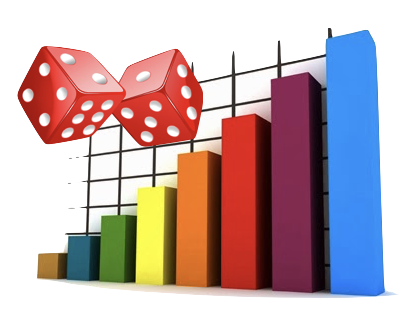
\includegraphics[width=4.5cm]{img-04/icono}}{chap:estadistica}


 \begin{iniaval}

\begin{itemize}
	\item 
 Hem tret aquestes notes d'exàmens de matemàtiques durant el curs: 
\begin{center}
 4 \quad\quad  7,5  \quad\quad  3   \quad\quad  6,2   \quad\quad  5   \quad\quad 4,75   \quad\quad 6,4  
 \end{center}
 Quina és la nota mitjana dels exàmens?
 

\item  Hem demanat el nombre de televisors que tenen les famílies d'un grup de 20 persones i hem obtingut aquests resultats:
\begin{center}
2  \quad 1 \quad 1 \quad 3  \quad2  \quad0  \quad1\quad 1 \quad 1 \quad 2 \quad 2 \quad 2  \quad3  \quad1 \quad 2\quad  1  \quad1  \quad2 \quad 4\quad2 
\end{center}
Construeix una taula de freqüències i dibuixa un diagrama de barres.

\begin{minipage}{0.5\textwidth}
	\begin{center}
	\begin{tabular}{c|c}
		$x$ & $f$	\\  \hline
		0 & 	\\  \hline
		1 & 	\\  \hline
		2 & 	\\  \hline
		3 & 	\\  \hline
		4 &  	
	\end{tabular}
\end{center}	
\end{minipage}
\begin{minipage}{0.5\textwidth}
	\begin{center}
		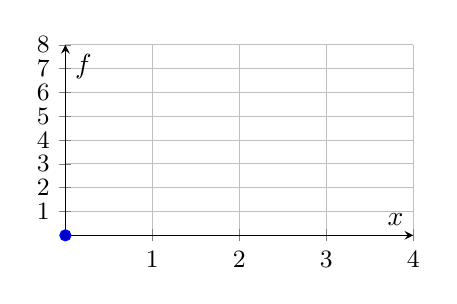
\begin{tikzpicture}
		\begin{axis}[width=6cm,height=4cm, axis background/.style={fill=white}, axis lines=middle, 
		grid = major,
		xlabel=$\small x$,
		ylabel=$\small f$, 
		xtick={0,1,2,3,4},
		ytick={0,1,2,3,4,5,6,7,8},
		tick label style={font=\small},
		xmin=0,
		xmax=4,
		ymax=8,
		legend style={font=\small,legend pos=outer north east},],
		\addplot coordinates {(0, 0)};
		\end{axis}
		
		\end{tikzpicture}
	\end{center}
\end{minipage}
  

\item Quina és la probabilitat de treure un 5 en llançar un dau? I de treure una carta d'oros d'una baralla espanyola?

\vspace{1cm}
\end{itemize}

\addanswersline[cols=1]{Avaluació inicial}{0}{[La mitjana és 5.2643, 
									 \begin{tabular}{c|c}
									 	x & f \\ \hline
									 	0 & 1  \\
									 	1 & 8  \\
									 	2 & 8 \\
									 	3 & 2 \\
									 	4 & 1 \\
									 \end{tabular} 
								 \par
								 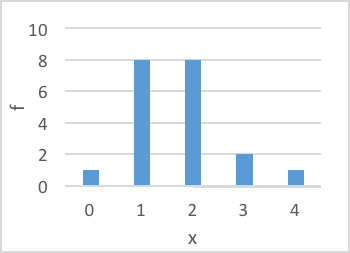
\includegraphics[width=0.4\textwidth]{img-sol/t4-0},
								$P(5)=\frac{1}{6}$ i 	$P(Oros)=\frac{10}{40}$]}

 \end{iniaval}
\newpage

\section{Fases d'un estudi estadístic}

\begin{theorybox}
 \textbf{Definicions:}

\begin{minipage}{0.7\textwidth}
		\begin{itemize}
	\item \textbf{      Individu: }Cadascun dels objectes que s'estudien.
	
	\item \textbf{      Població: }Conjunt de tots els individus que s'estudien.
	
	\item \textbf{      Mostra:} Part de la població de la qual es prendran dades.
	\end{itemize}

\vspace{0.25cm}

	 \textbf{Variable estadística. }És l'aspecte de l'estudi i es\textbf{ classifica en:}
	\begin{itemize}
		\item \textbf{       Qualitativa:} Expressa una qualitat, com ara color, marca, etc.
		\item \textbf{        Quantitativa: }S'expressa amb un nombre.  
		\begin{itemize}
			\item \textbf{Discreta} (el nombre és enter) 
			\item \textbf{Contínua} (el  nombre pot contenir decimals).
		\end{itemize}
	\end{itemize}
\end{minipage}
\begin{minipage}{0.3\textwidth}
	\centering
	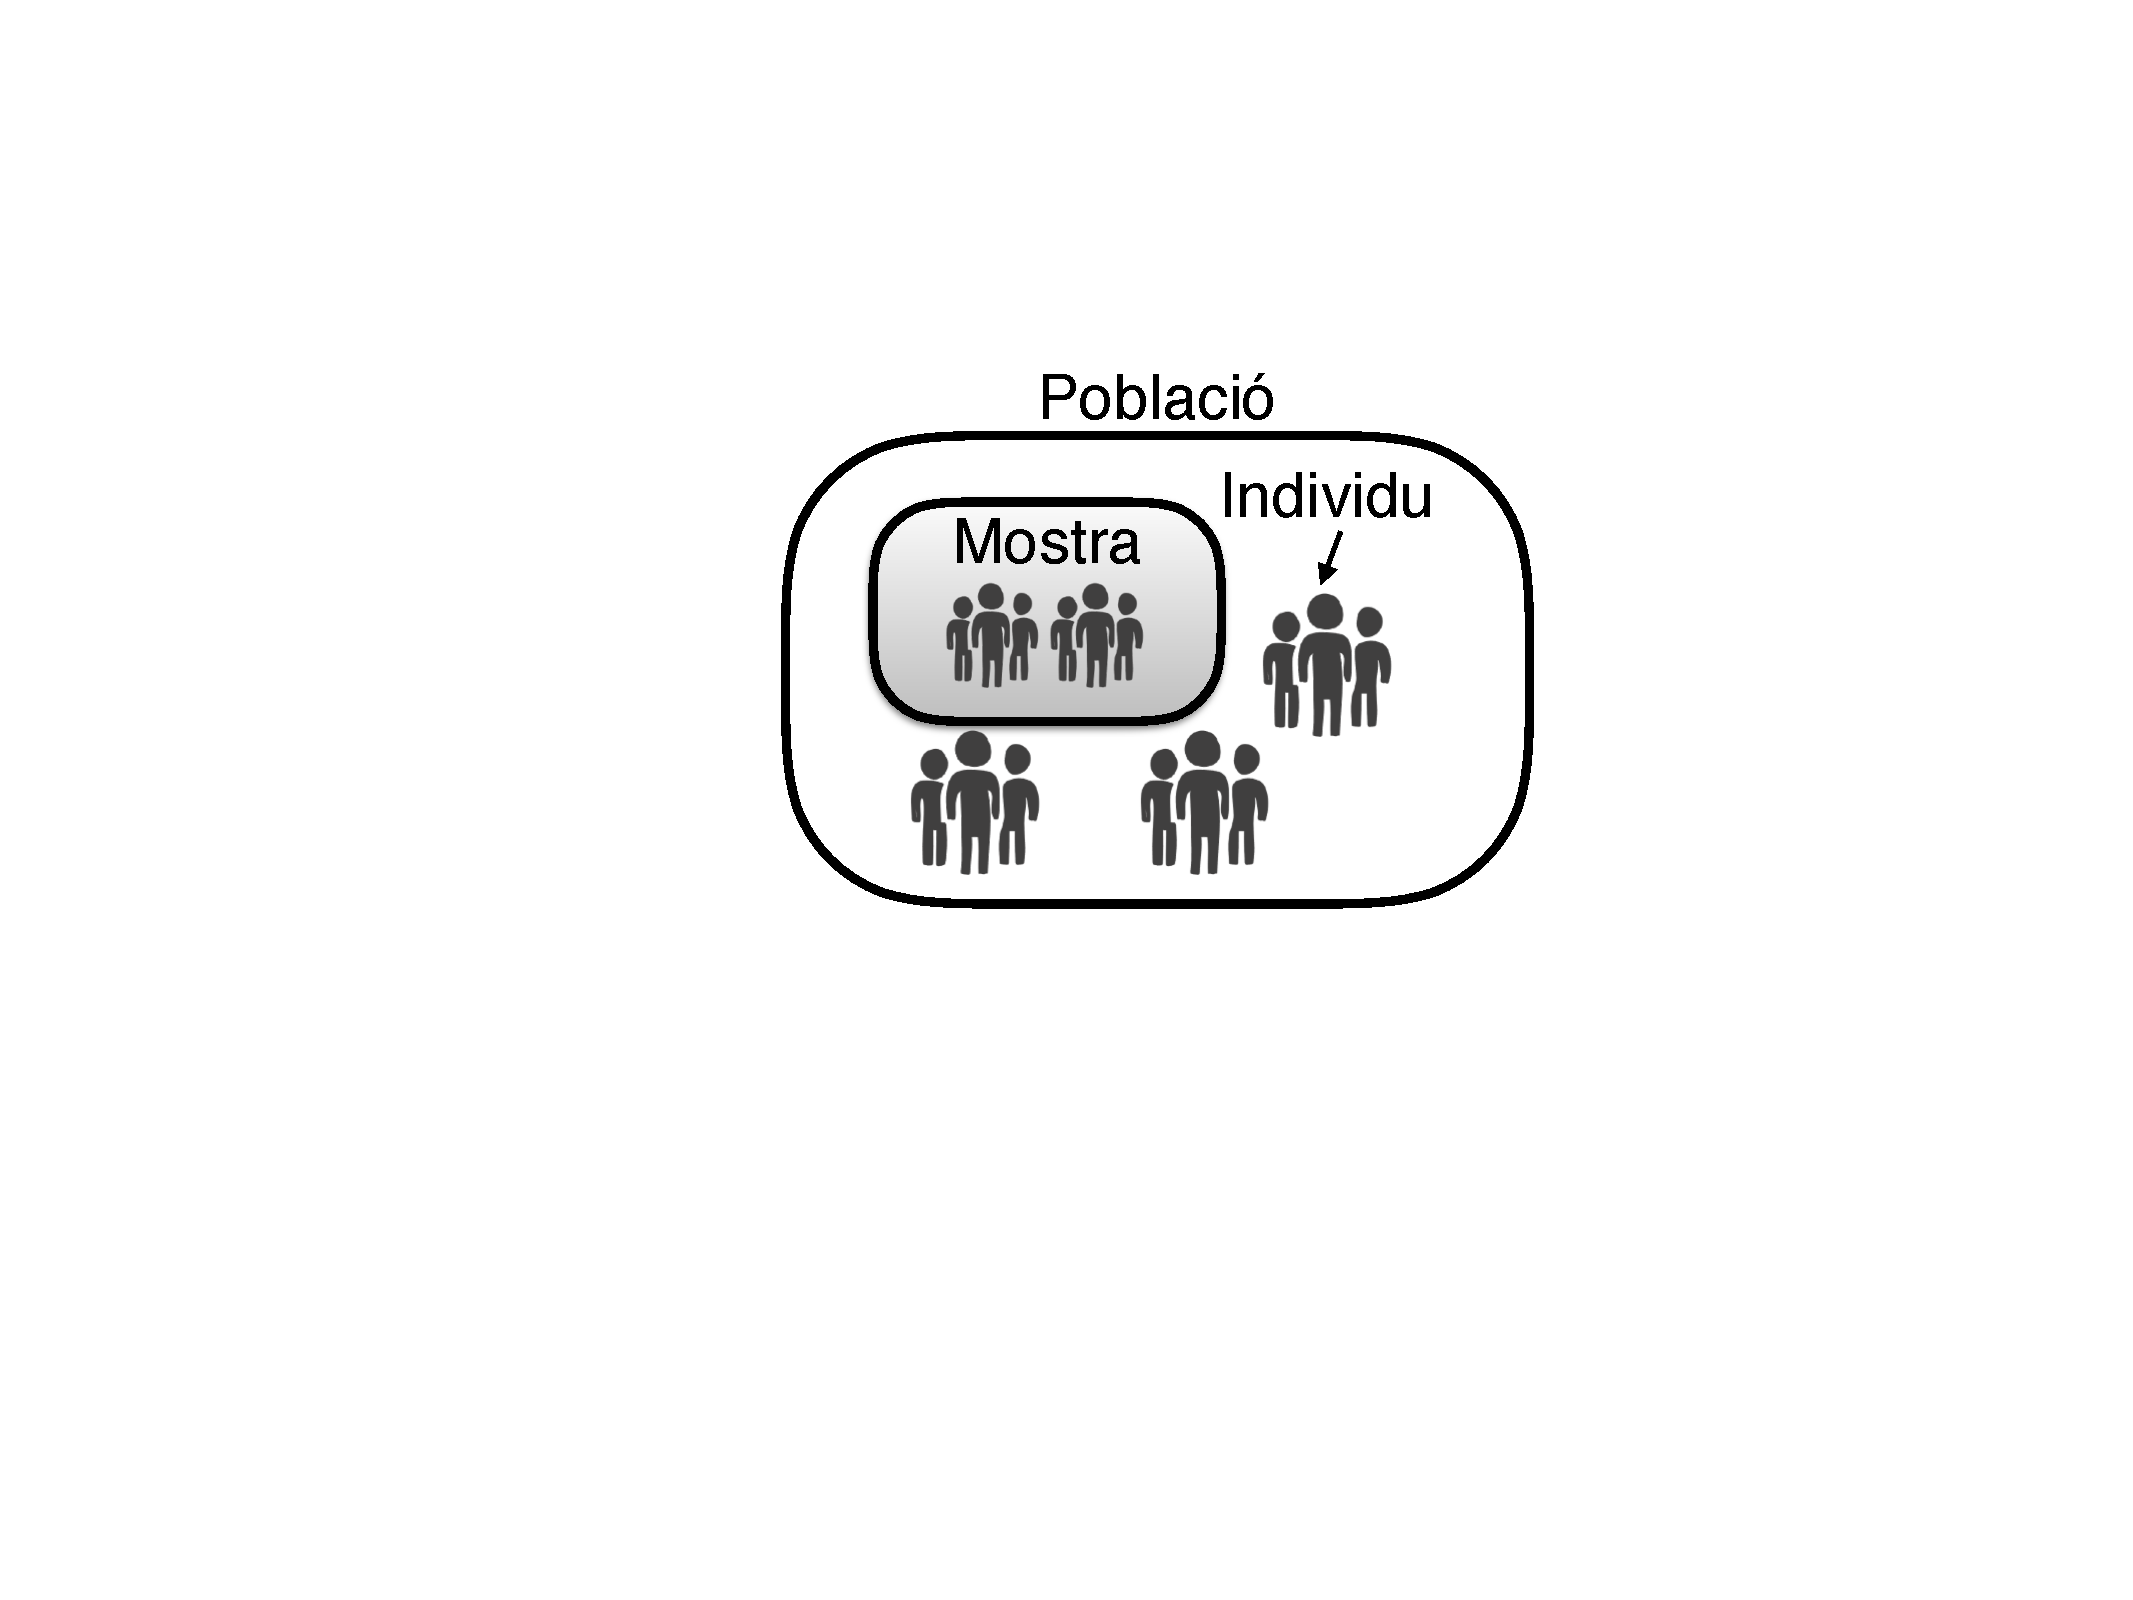
\includegraphics[width=0.9\textwidth]{img-04/mostra}
\end{minipage}




 \textbf{Fases d'un estudi estadístic:}
\begin{enumerate} 
	\item Tenir clara la pregunta i el tipus de variable estadística que es vol estudiar.  
	\item Prendre una mostra representativa.
	\item Recollir les dades (fent una enquesta, etc.) 
	\item  Fer un recompte de dades, càlculs de paràmetres estadístics i gràfics.
	\item Treure conclusions.
\end{enumerate} 
\end{theorybox}

\begin{mylist}

\exer Volem fer un estudi de la quantitat de monedes que duen a la butxaca els estudiants de la classe. Però, per no demanar a tots triam 10 companys a l'atzar i anotam en el quadern quantes monedes duu cadascun.

\begin{tasks}
	\task Quina és la població objecte de l'estudi?
	\task Quina és la mostra triada?
	\task Especifica 5 individus que pertanyin a la població i no a la mostra.
\end{tasks}
 
\answers[cols=1]{[La població són tots els alumnes de la classe, La mostra són els 10 companys triats a l'atzar, Qualssevol alumne de la classe que no hagués estat triat a l'atzar.]}
 
\exer \spen Classifica en variables qualitatives i quantitatives. Per a les quantitatives indica si són contínues o discretes.
\begin{tasks}
\task Quines fruites menges al llarg d'una setmana? \dotfill\hspace{1cm}
\task  Quantes peces de fruita menges al dia? \dotfill\hspace{1cm}
\task  Quantes monedes portes en la butxaca? \dotfill\hspace{1cm}
\task  Quina és la teva altura? \dotfill\hspace{1cm}
%\task  Quantes marques de xocolata recordes?
\task  Quines són les marques de xocolata que recordes? \dotfill\hspace{1cm}
\task  Quants germans tens? \dotfill\hspace{1cm}
\task  Quin és el teu color favorit per a un cotxe? \dotfill\hspace{1cm}
\task  Quant temps passes al dia veient la televisió? \dotfill\hspace{1cm}
\task  Quants seguidors tens en twitter? \dotfill\hspace{1cm}
\end{tasks}
\answers[cols=1]{[Qualitativa, Quantitativa Discreta, Quantitativa Discreta, Quantitativa Contínua, Qualitativa, Quantitativa Discreta, Qualitativa, Quantitativa Contínua, Quantitativa Discreta]}
 

 \exer Assenyala en quin cas és més convenient estudiar la població o una mostra:
\begin{tasks}
 \task El diàmetre dels cargols que fabrica una màquina diàriament. 
%
 \task L'altura d'un grup de sis amics. 
\end{tasks}
\answers[cols=1]{[Millor la mosta, Millor la població]}
 

 \exer Es pot llegir el següent titular en la revista que publica el teu institut: ``\textit{La nota mitjana dels alumnes de 3r ESO és }de 7,9''. Com s'ha arribat a aquesta conclusió? S'ha estudiat a tota la població? Si haguessin seleccionat per al seu càlcul tan sols a les nines, seria representatiu el seu valor?

 \answers{Segurament hauran utilitzat el programa Gestib que ho gestiona tot. En tal cas, estudien tota la població. Si l'estudi
 hagués comptat només amb les alumnes, el resultat no representaria a toda la població.}

 \exer En una sèrie de televisió tenen dubtes sobre què fer amb la protagonista, si que tingui un accident o si ha de casar-se. Volen fer una consulta; a tota la població o seleccionat una mostra representativa? Raona la resposta.

\answers{Seria molt complicat consultar a tota la població (llarg i car). Millor una mostra.}

\end{mylist}

\section{Representació de la informació}

\begin{center}
\boxed{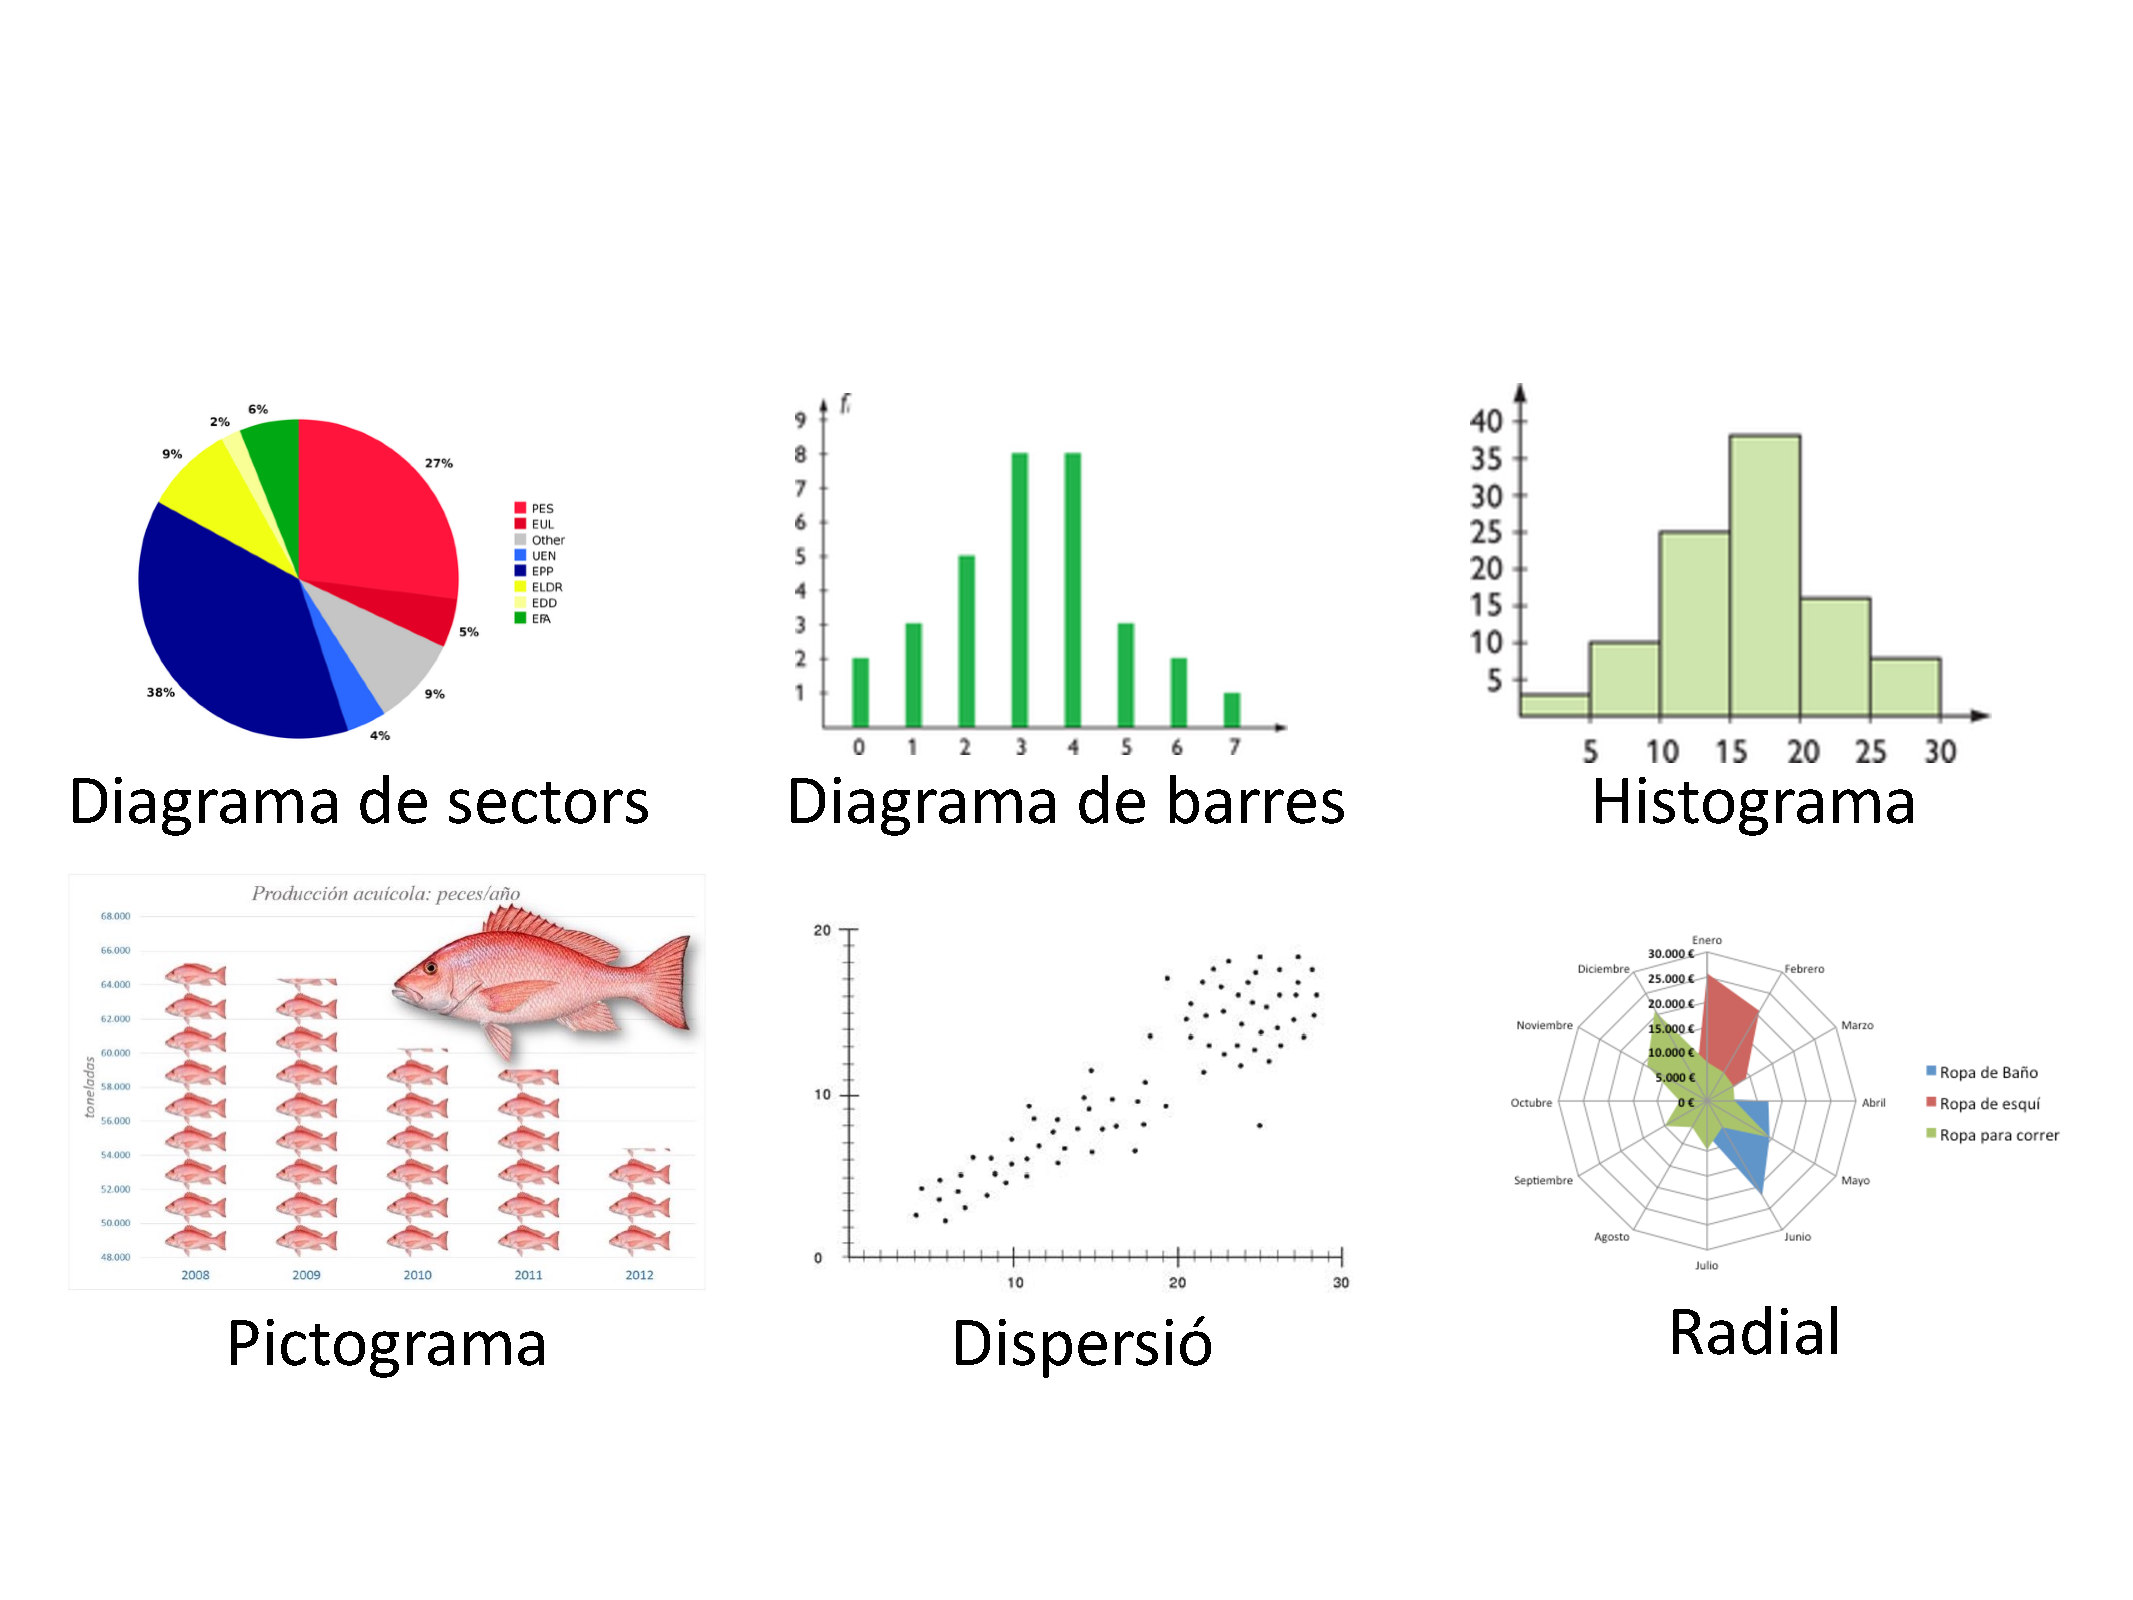
\includegraphics[width=0.9\textwidth]{img-04/grafics}}
\end{center}

\begin{mylist}
 \exer  Reuneix a 10 companys. Compta quantes monedes de cada valor (1 cèntim, 2 cèntims, 5 cèntims, {\dots}) teniu entre tots. Representa mitjançant un gràfic adequat el nombre de monedes de cada tipus que teniu. Hi ha algun altre diagrama que et permeti veure quin tipus de monedes són més abundants en la mostra que has pres?

\answers{Solució oberta. Faríem un diagrama de sectors o de barres.}
  
 \exer En la classe d'Educació Física el professor ha mesurat el temps que tarda cada alumne a recórrer 100 metres. Els resultats estan en aquesta taula:
\begin{center}
\begin{tabular}{|p{0.4in}|p{0.4in}|p{0.4in}|p{0.4in}|p{0.4in}|p{0.4in}|p{0.4in}|p{0.4in}|} \hline 
14'92 & 13'01 & 12'22 & 16'72 & 12'06 & 10'11 & 10'58 & 18'58 \\ \hline
20'07 & 13'15 & 20'10 & 12'43 & 17'51 & 11'59 & 11'79 & 16'94 \\ \hline
16'45 & 10'94 & 16'56 & 14'87 & 17'59 & 13'74 & 19'71 & 18'63 \\ \hline
19'87 & 11'12 & 12'09 & 14'20 & 18'30 & 17'64 & &\\ \hline 
\end{tabular}
\end{center}
Agrupa aquests resultats en intervals començant en 10 segons i de longitud 1 segon. Realitza una taula de freqüències i representa adequadament aquestes dades.

\answers{
\begin{tabular}{c|c}
Interval & f \\ \hline
10 -- 11 &   3    \\ 
11 -- 12 &   3 \\ 
12 -- 13&   4 \\ 
13 -- 14&   3 \\ 
14 -- 15&   3 \\ 
15 -- 16&   0 \\ 
16 -- 17&   4 \\ 
17 -- 18&   3 \\ 
18 -- 19&   3 \\ 
19 -- 20 &  2  \\
20 -- 21 & 2 \\ \hline
 & 30 \\ 
\end{tabular}
\par
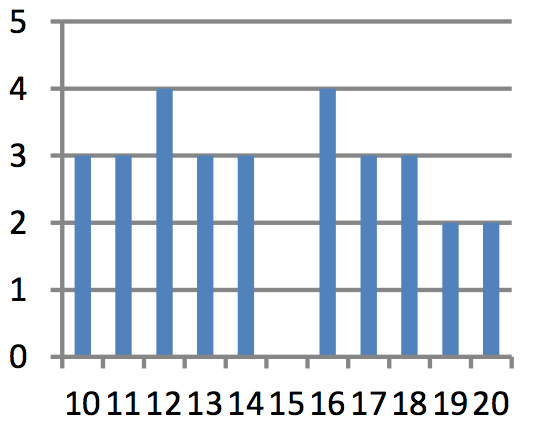
\includegraphics[width=0.35\textwidth]{img-sol/t4-7}
\par \ggblink{https://goo.gl/pWA3K9}
}

\end{mylist}


\section{Paràmetres estadístics}
\begin{theorybox}[Paràmetres estadístics]
	Donada una variable estadística $x_i$ amb cada valor repetit $f_i$ vegades (freqüència), es defineixen	
	
	\begin{minipage}{0.45\textwidth}
	\begin{itemize}
		\item \textbf{Nombre de dades:} $N=\sum_i f_i$
		\item \textbf{Mitjana aritmètica:} $\bar x=\dfrac{\sum_i f_i x_i}{N}$
		\item \textbf{Variància:} $Var=\dfrac{\sum_i f_i x^2_i}{N}-\bar x^2$
		\item \textbf{Desviació típica:} $\sigma=\sqrt{Var}$		
		\item \textbf{Coeficient de variació:} $CV = \dfrac{\sigma_x}{\bar x}$
	\end{itemize}
	\end{minipage}
	\hspace{0.3cm}
	\begin{minipage}{0.44\textwidth}
				\begin{itemize}
				\item \textbf{Moda:} El valor de $x$ més freqüent.
				\item \textbf{Mediana:} Valor de $x$ pel qual la {\normalfont \textit{freqüència acumulada}} assoleix el 50\%.
				\item \textbf{Rang:} La diferència entre els valors major i menor de $x$.
				 
			\end{itemize}
	\end{minipage}
	
	La mitjana és el centre de gravetat de la distribució i la desviació típica ens dóna la \textbf{dispersió}. És a dir, ens diu com d'allunyades estan les dades respecte de la mitjana. 
	Podem pensar que una dada és ``normal'' si es troba dins l'interval de $x$ $(\bar x -\sigma, \bar x + \sigma)$.
\end{theorybox}
	
	\begin{resolt}{Hem demanat pel nombre d'assignatures suspeses a un grup de 15 alumnes i aquestes han estat les respostes:\vspace{0.25cm}
			 \begin{center}
			 \begin{tabular}{cccc}
			 	1 & 0 & 3 & 2 \\
			 	0 & 6 & 2 & 5 \\
			 	3 & 2 & 4 & 3 \\
			 	4 & 1 & 3 & 	
			 \end{tabular}
		\end{center}
		\vspace{0.25cm}
		
			\begin{itemize}
				\item[a)]  Fes un recompte i dibuixa un diagrama de barres.
				
				\item[b)]  Calcula la mitjana i la desviació típica.
			\end{itemize}
		}
		
\begin{center}
\begin{minipage}{0.2\textwidth}
	\centering
	 	\begin{tabular}{|p{0.4in}|p{0.4in}|} \hline 
			$x_i$ & $f_i$ \\ \hline 
			0 & 2\\ \hline 
			1 & 2 \\ \hline 
			2 & 3 \\ \hline 
			3 & 4 \\ \hline 
			4 & 2 \\ \hline 
			5 & 1 \\ \hline 
			6 & 1  \\ \hline
		\end{tabular}
\end{minipage}	
\begin{minipage}{0.4\textwidth} 
	\centering
	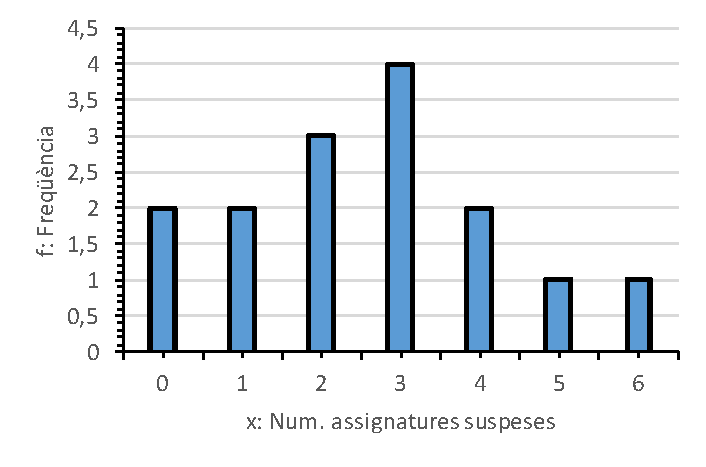
\includegraphics[width=\textwidth]{img-04/histo2}
\end{minipage}
\end{center}

		\vspace{0.24cm}
		
		Per calcular els paràmetres estadístics necessitam calcular dues columnes més $f\cdot x$ i $f\cdot x^2$:
		\begin{center}
			\begin{tabular}{|p{0.7in}|p{0.8in}|p{0.8in}|p{0.8in}|} \hline 
				$x_i$ & $f_i$ & $f_i x_i$ & $f_i x_i^2$\\ \hline 
				0 & 2 & 0 & 0 \\ \hline 
				1 & 2 & 2 & 2 \\ \hline 
				2 & 3 & 6 & 12\\ \hline 
				3 & 4 & 12 & 36 \\ \hline 
				4 & 2 & 8 &  32\\ \hline
				5 & 1 & 5 &  25\\ \hline
				6 & 1 & 6 &  36\\ \hline\hline
				\rowcolor{lightgray} SUMES & 15 &  39  & 143 \\ \hline 
			\end{tabular}
		\end{center}	\vspace{0.24cm}
		
		La mitjana s'obté de $\bar x = \dfrac{39}{15}=2.6$
		
		La desviació típica  $\sigma = \sqrt{ \dfrac{143}{15}-2.6^2 }=1.67$
		
		El coeficient de variació és $CV = \dfrac{1.67}{2.6}=0.64$, aproximadament un 64\%.
		
	\end{resolt}
	\vspace{1cm}
	
	\newpage
	
	
	\begin{resolt}{En un barri s'ha trobat que les famílies residents s'han distribuït, segons el número de membres, de la forma següent:\vspace{0.25cm}
			
			\begin{tabular}{|p{0.7in}|p{0.8in}|} \hline 
				\textbf{\textit{membres}} & \textbf{\textit{nº famílies}} \\ \hline 
				0-2 & 110 \\ \hline 
				2-4 & 200 \\ \hline 
				4-6 & 90 \\ \hline 
				6-8 & 75 \\ \hline 
				8-10 & 25 \\ \hline 
			\end{tabular}
			\vspace{0.25cm}
			
			\begin{itemize}
				\item[a)]  Representa un histograma.
				
				\item[b)]  Calcula la mitjana i la desviació típica.
			\end{itemize}
		}
		
		\begin{wrapfigure}{R}{0.3\textwidth} 
			\vspace{-0.75cm}
			\begin{center}
				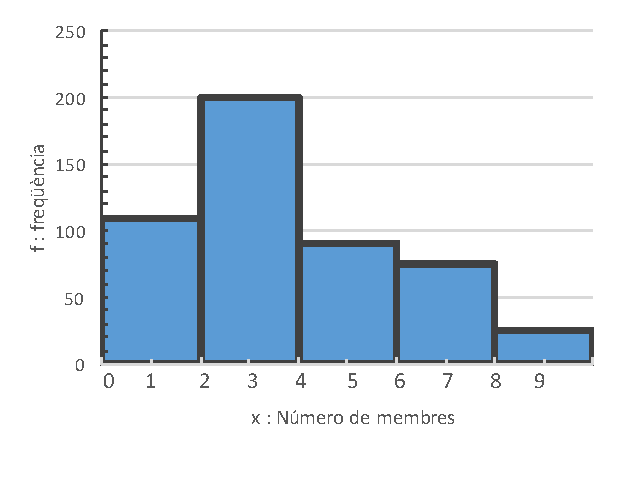
\includegraphics[width=0.26\textwidth]{img-04/histo1}
			\end{center}
			\vspace{-0.5cm}
		\end{wrapfigure}
		
		a)
		\vspace{0.24cm}
		
		Es tracta d'una variable discreta (número de membres) que s'ha agrupat en intervals. El número de famílies és la freqüència. Aleshores, el gràfic més adequat és fer un histograma.
		\vspace{0.24cm}
		
		Per calcular els paràmetres estadístics necessitam calcular \textbf{la marca de classe} que és el punt mitjà de cada interval.
		\begin{center}
			\begin{tabular}{|p{0.7in}|p{0.8in}|p{0.8in}|p{0.8in}|} \hline 
				$x_i: marca$ & $f_i$ & $f_i x_i$ & $f_i x_i^2$\\ \hline 
				1 & 110 & 110 & 110 \\ \hline 
				3 & 200 & 600 & 1800 \\ \hline 
				5 & 90 & 450 & 2250\\ \hline 
				7 & 75 & 525 & 3675 \\ \hline 
				9 & 25 & 225 & 2025 \\ \hline\hline
				\rowcolor{lightgray} SUMES & 500 & 1910 & 9860\\ \hline 
			\end{tabular}
		\end{center}	\vspace{0.24cm}
		
		b)
		\vspace{0.24cm}
		
		
		La mitjana s'obté de $\bar x = \dfrac{1910}{500}=3.82$
		
		La desviació típica  $\sigma = \sqrt{ \dfrac{9860}{500}-3.82^2 }=2.26$
		
		El coeficient de variació és $CV = \dfrac{2.26}{3.82}=0.57$, aproximadament un 60\%.
		
	\end{resolt}
	\vspace{1cm}

\begin{mylist}
	
\exer[1]  En una excursió de muntanya participen 25 persones amb les següents edats: 
\begin{center}
	\begin{tabular}{|p{0.27in}|p{0.27in}|p{0.27in}|p{0.27in}|p{0.27in}|p{0.27in}|p{0.27in}|p{0.27in}|p{0.27in}|p{0.27in}|p{0.27in}|p{0.27in}|p{0.27in}|} \hline
		8 & 10 & 10 & 11& 12& 36& 37& 37& 38& 40& 42& 43& 43 \\ \hline  
		44 & 45 & 47 & 48& 50& 52& 53& 55& 58& 61& 63& 67&  \\ \hline 
\end{tabular}
\end{center}
\begin{tasks}
\task Fes una taula de freqüències classificant les edats en 6 intervals que comencen en 7,5 i acaben en 67,5. Troba, a partir de la taula, els paràmetres $\bar{x}$, $\sigmaup$  i CV.
\task Calcula $\bar{x}$, $\sigmaup$  i CV  introduint els 25 dades en la calculadora, és a dir, sense agrupar-los en intervals.
\task Prescindint dels 5 nins, obtenim un col·lectiu de 20 persones. Calcula de nou els seus paràmetres $\bar{x}$, $\sigmaup$ i CV,  i compara amb els obtinguts en el grup inicial.
\end{tasks}

\answers[cols=1]{[$\bar x=40.5$; $\sigma=16.5$; $CV=0.407$,  $\bar x=40.4$; $\sigma=17.11$; $CV=0.424$, $\bar x=46.5$; $\sigma=9.74$; $CV=0.21$ \par \ggblink{https://goo.gl/JfqFSu}]}

\end{mylist}


\newpage

 \section{Problemes d'estadística}

\begin{mylist}
	
 \exer[1] S'han recollit les dades sobre el nombre de fills que tenen 20 matrimonis. Com és la variable utilitzada? Escriu una taula de freqüències de les dades recollides i representa les dades en un diagrama de sectors:  
\begin{center}
3, \quad 1,\quad 1, \quad2,\quad0, \quad2, \quad3, \quad1,\quad 1,\quad 1,\quad 1, \quad0, \quad3, \quad2, \quad1,\quad 2,\quad 1,\quad 2,\quad 2,\quad 3
\end{center}
 Amb aquestes dades calcula la moda, la mitjana, la variància i la desviació típica. 
  
\answers{$M_o =1$; $\bar x=1.6$; $Var=0.84$; $\sigma=0.92$\par
\ggblink{https://goo.gl/nKce19}}

\vso

 \exer[1] Es demana a un grup de persones pel nombre de televisors que hi ha en casa seva i els resultats han estat: 

\begin{longtable}{|p{1.2in}|p{0.2in}|p{0.2in}|p{0.2in}|p{0.2in}|p{0.2in}|p{0.2in}|} \hline 
Nombre de \par televisors & 0 & 1 & 2 & 3 & 4 & 5 \\ \hline 
Nombre de llars & 2 & 27 & 15 & 4 & 2 & 1 \\ \hline 
\end{longtable}

Quin tipus de variable és? Representa les dades en la representació que et sembli més adequada. Calcula la mitjana i la desviació típica.

\answers{Variable quantitativa discreta;\par $\bar x=1.6078$; $\sigma=0.9717$\par \ggblink{https://goo.gl/9tu6n7}}

\vso

\exer[1] En un centre escolar s'ha recollit informació sobre el nombre d'ordinadors a les cases de 100 famílies i s'han obtingut els següents resultats: 

\begin{longtable}{|p{1.3in}|p{0.3in}|p{0.3in}|p{0.3in}|p{0.3in}|p{0.3in}|} \hline 
Nombre \par d'ordinadors & 0 & 1 & 2 & 3 & 4 \\ \hline 
Nombre de \par famílies: & 24 & 60 & 14 & 1 & 1 \\ \hline 
\end{longtable}

Representa les dades en un diagrama de barres i calcula la mitjana, la mediana i la moda.
\answers{$\bar x=0.95$;  $M_o=1$; $M_e$ = 1; $Q_1 = 1$; $Q_3= 1$
	\par
	\ggblink{https://goo.gl/nFytiW}
}
 
\exer Amb les dades del problema anterior calcula el rang, la desviació mitjana, la variància i la desviació típica. 


\answers{Rang = 4. Desviació mitjana = 0,456. Variància = 0,299. Desviació típica = 0,5473; \par \ggblink{https://goo.gl/nFytiW}}

\vso

 \exer Es demana a un grup de persones pel nombre de vegades que han visitat al dentista en l'últim any. Les respostes obtingudes es recullen en la següent taula: 

\begin{longtable}{|p{1.5in}|p{0.5in}|p{0.5in}|p{0.5in}|p{0.5in}|p{0.5in}|} \hline 
Nombre de visites: & 1 & 2 & 3 & 4 & 5 \\ \hline 
Nombre de persones: & 13 & 18 & 7 & 5 & 7 \\ \hline 
\end{longtable}

\begin{tasks}
	\task Representa les dades en un diagrama de sectors i calcula la mitjana, la mediana i la moda.
	\task Calcula el rang, la desviació mitjana, la variància i la desviació típica.	
\end{tasks}

\answers{[Mitjana = 2.5; Mediana = 2; Moda = 2; Var=1.81; $\sigma=1.345$;  CV=0.538, 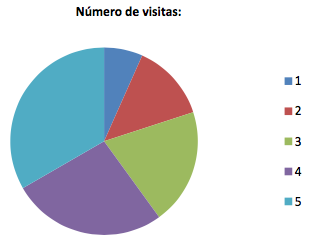
\includegraphics[width=0.35\textwidth]{img-sol/t4-13}\par \ggblink{https://goo.gl/RtMKif}]}
 
\newpage

\exer  En un control de velocitat en carretera s'obtingueren les dades següents

\begin{longtable}{|p{1.3in}|p{0.5in}|p{0.5in}|p{0.5in}|p{0.5in}|p{0.7in}|p{0.7in}|} \hline 
Velocitat (km/h): & 60--70 & 70--80 & 80--90 & 90--100 & 100-110 & 110-120 \\ \hline 
Nombre de cotxes: & 5 & 15 & 27 & 38 & 23 & 17 \\ \hline 
\end{longtable}

\begin{tasks}
	\task Calcula la mitjana i la desviació típica de la velocitat dels cotxes. {\textit Ajuda: } La marca de classe de l'interval 60--70 és 65.
	\task Quin percentatge circula a més de 90 km/h?
\end{tasks}
 
 \answers{[$\bar x=93.8$; $\sigma=13.3$; $CV=0.142$,  62.4 \% \par \ggblink{https://goo.gl/t62BLv}]}

\vso
\exer  La següent taula expressa les alçades, en metres, de 1000 soldats: 

\begin{longtable}{|p{0.9in}|p{0.5in}|p{0.5in}|p{0.5in}|p{0.5in}|p{0.5in}|p{0.5in}|} \hline 
Talla & 1,50 -- 1,56 & 1,56 -- 1,62 & 1,62 -- 1,68 & 1,68 - 1,74 & 1,74 - 1,80 & 1,80-1,86 \\ \hline 
Nº de soldats & 10 & 140 & 210 & 340 & 210 & 90 \\ \hline 
\end{longtable}

\begin{tasks}
	\task Representa les dades en un histograma.
	\task Calcula la mitjana i la desviació típica. 
	\task Determina l'interval on es troba la mediana.
\end{tasks}
\answers{[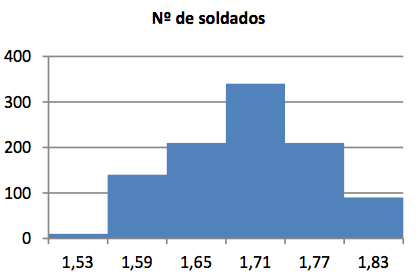
\includegraphics[width=0.35\textwidth]{img-sol/t4-15},
		Mitjana = 1.7049. Desviació típica =0.07132,
Mediana. Per a calcular l'interval on es troba miram, en
 la taula de les freqüències acumulades, estan els 500 soldats. És l'interval 1,68 – 1,74.\par 
 \ggblink{https://goo.gl/QVSssH}
 ]}
 

 \begin{comment}
 \exer En les eleccions de 2014 al Parlament Europeu es van obtenir els següents escons per grup parlamentari (DM: demòcrata -- cristians; S: socialistes; L: Liberals; V: verds; C: conservadors; I: esquerra unitària; LD: Llibertat i democràcia; NI: No inscrits; Uns altres). 

\begin{longtable}{|p{0.7in}|p{0.3in}|p{0.3in}|p{0.3in}|p{0.3in}|p{0.3in}|p{0.3in}|p{0.3in}|p{0.3in}|p{0.4in}|p{0.4in}|} \hline 
Partits & DM & S & L & V & C & I & LD & NI & Uns altres & Total \\ \hline 
Escons & 213 & 190 & 64 & 52 & 46 & 42 & 38 & 41 & 65 & 751 \\ \hline 
\end{longtable}

Quina representació de les dades et sembla més adequada? Pots calcular la mitjana o el rang? Quin tipus de variables és la de la taula?


\exer  En les eleccions de 2014 al Parlament Europeu es van obtenir els següents escons per algun dels estats membre: 

\begin{longtable}{|p{0.5in}|p{0.5in}|p{0.5in}|p{0.5in}|p{0.5in}|p{0.5in}|p{0.5in}|p{0.5in}|p{0.5in}|p{0.5in}|p{0.5in}|} \hline 
Estat & Alemanya & Espanya & França & Itàlia & Polònia & Regne Unit & Portugal & Grècia & Uns altres & Total \\ \hline 
Escons & 96 & 54 & 74 & 73 & 51 & 73 & 21 & 21 &  & 751 \\ \hline 
\end{longtable}

Quina representació de les dades et sembla més adequada? Pots calcular la mitjana o el rang? Quin tipus de variables és la de la taula? Determina el nombre d'escons dels altres països membres de la Unió Europea.
\end{comment}

\vso
 \exer En les eleccions de 2004, 2009, 2014 al Parlament Europeu es van obtenir els següents percentatges de vots per alguns dels estats membres: 

\begin{longtable}{|p{0.4in}|p{0.6in}|p{0.5in}|p{0.4in}|p{0.4in}|p{0.4in}|p{0.5in}|p{0.4in}|p{0.5in}|p{0.5in}|} \hline 
Estat & Alemanya & Espanya & França & Itàlia & Regne Unit & Portugal & Grècia & Bèlgica & \% total \\ \hline 
2004 & 43 & 45'14 & 42'76 & 71'72 & 38'52 & 38'6 & 63'22 & 90'81 & 45'47 \\ \hline 
2009 & 43'27 & 44'87 & 40'63 & 65'05 & 34'7 & 36'77 & 52'61 & 90'39 & 43 \\ \hline 
2014 & 47'6 & 45'9 & 43'5 & 60 & 36 & 34'5 & 58'2 & 90 & 43'09 \\ \hline 
\end{longtable}

Quina representació de les dades et sembla més adequada? Pots calcular la mitjana o el rang? Quin tipus de variables és la de la taula? Ordena als països de major a menys percentatge de votants en les eleccions de 2014.
\vso
\answers{Es pot representar mitjançant un diagrama de barres amb colors diferents per a cada any. La variable és
	quantitativa contínua i es poden calcular paràmetres estadístics. L'ordre dels països és Bèlgica$>$
	Itàlia $>$ Grècia $>$ Espanya $>$ Alemanya $>$ França $>$ Portugal $>$ Regne Unit.\par  
\ggblink{https://goo.gl/Z6UoWb}}

\exer  En les eleccions de 2014 al Parlament Europeu els resultats d'Espanya han estat: 

\begin{longtable}{|p{0.9in}|p{0.9in}|p{0.9in}|p{0.9in}|p{0.9in}|} \hline 
Cens & Total de votants & Abstenció & Vots nuls & Vots en blanc \\ \hline 
35.379.097 & 15.620.815 & 19.058.282 & 290.189 & 409.811 \\ \hline 
\end{longtable}

Representa en un diagrama de sectors aquestes dades. Fes una taula de percentatges: el cens és el 100 \%. Determina els altres percentatges. Consideres que ha guanyat l'abstenció?

\answers{ 
	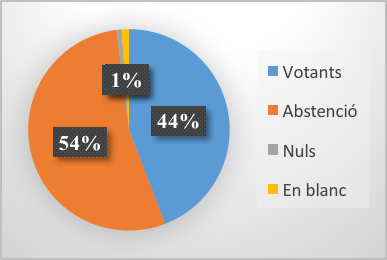
\includegraphics[width=0.4\textwidth]{img-sol/t4-17}
	 \par
	Cens=100 \%;\par
	Total de votants=
	44,152 \%; \par
	Abstenció=
	53,87 \%; \par
	Vots nuls=
	0,82022727 \%; \par
	Vots en blanc=
	1,1583\%; \par
	Ha guanyat l'abstenció, amb més de la meitat del cens.\par 
\ggblink{https://goo.gl/JjcnL4}}
   
\begin{comment}
 \exer En les eleccions de 2014 al Parlament Europeu els resultats d'Espanya han estat: 

\begin{longtable}{|p{0.7in}|p{0.7in}|p{0.7in}|p{0.7in}|p{0.7in}|p{0.7in}|p{0.7in}|} \hline 
\textbf{PP} & \textbf{PSOE} & \textbf{Esquerra plural} & \textbf{Podemos} & \textbf{UPyD} & \textbf{Uns altres} & \textbf{Total de votants} \\ \hline 
4.074.363 & 8.001.754 & 1.562.567 & 1.245.948 & 1.015.994 &  & 15.920.815 \\ \hline 
\end{longtable}

Determina el nombre de vots dels altres partits. Representa en un diagrama de barres aquestes dades. Fes una taula de percentatges per a cada partit. Has de distribuir 54 escons, com els distribuiries per partits?
\end{comment}
\end{mylist} 

\newpage

\section{Introducció al càlcul de probabilitats}
\begin{theorybox}
 \video[ytid=R9ZSI6Rq9Yw]{155}{Introducció a la probabilitat}

                 - Experiències deterministes i \textbf{aleatòries} (hi intervé l'atzar).                                     
                 
                 \textbf{- Espai Mostral E}: Conjunt de tots els possibles resultats d'un experiment aleatori.

 La \textbf{probabilitat} és una mesura de quant freqüent és un \textbf{succés}. Es quantifica amb un nombre que com a mínim val 0 (succés impossible) i com a màxim 1 (succés segur).

 La probabilitat (experimental) és el valor de la \textbf{freqüència relativa} (freqüència / nombre de repeticions) quan repetim l'experiment moltes vegades.

 Si $S'$ i $S$ són \textbf{successos contraris}, es compleix que $P(S')=1-P(S)$.
\end{theorybox}
                                               
\begin{mylist}
\exer \mental Per a cadascun d'aquests experiments indica si és determinista o aleatori.
\begin{tasks} 
	\task  Treim una carta a l'atzar d'una baralla espanyola i mirem el pal.
	\task  Treim una bola d'una bossa que només conté boles vermelles i miram el color.
	\task  Mesurem la quantitat de gasoil que cap en dipòsit el nostre cotxe.
	\task  Cronometram el temps que tardam d'anar de casa al col·legi en diferents dies.
	\task  Llancem dos daus i mirem si ha sortit igual puntuació en els dos.
\end{tasks}
\answers[cols=1]{[Aleatori, Determinista, Determinista, Aleatori, Aleatori]}

\exer  Una baralla francesa té 52 cartes, distribuïdes en 13 cartes de piques, 13 de cors, 13 de trèvols i 13 de diamants. Les piques i els trèvols són cartes negres mentre que els cors i els diamants són cartes vermelles. Es barreja la baralla, es talla i es fa el següent experiment: agafar les dues cartes que han quedat a dalt del tot i observar de quin color són. Descriu l'espai mostral. 
\answers{E=$\{VV, VN, NV, NN \}$}
  
\vspace{-2cm}
\exer \simbolsearch \begin{minipage}[t]{0.7\textwidth} \textit{\bf Experiment llançament de monedes}. Agafa una moneda d'un euro per exemple. Primer de tot, decideix quina banda és cara (C) i quina creu (X). Ara llança la moneda 10 vegades i compta quantes cares han sortit.  Tot seguit, el professor anirà demanant a cada grup quins han estat els resultats i els apuntarem en aquesta taula
	\end{minipage}
\begin{minipage}{0.3\textwidth}
	\vspace{2cm}
	\centering
	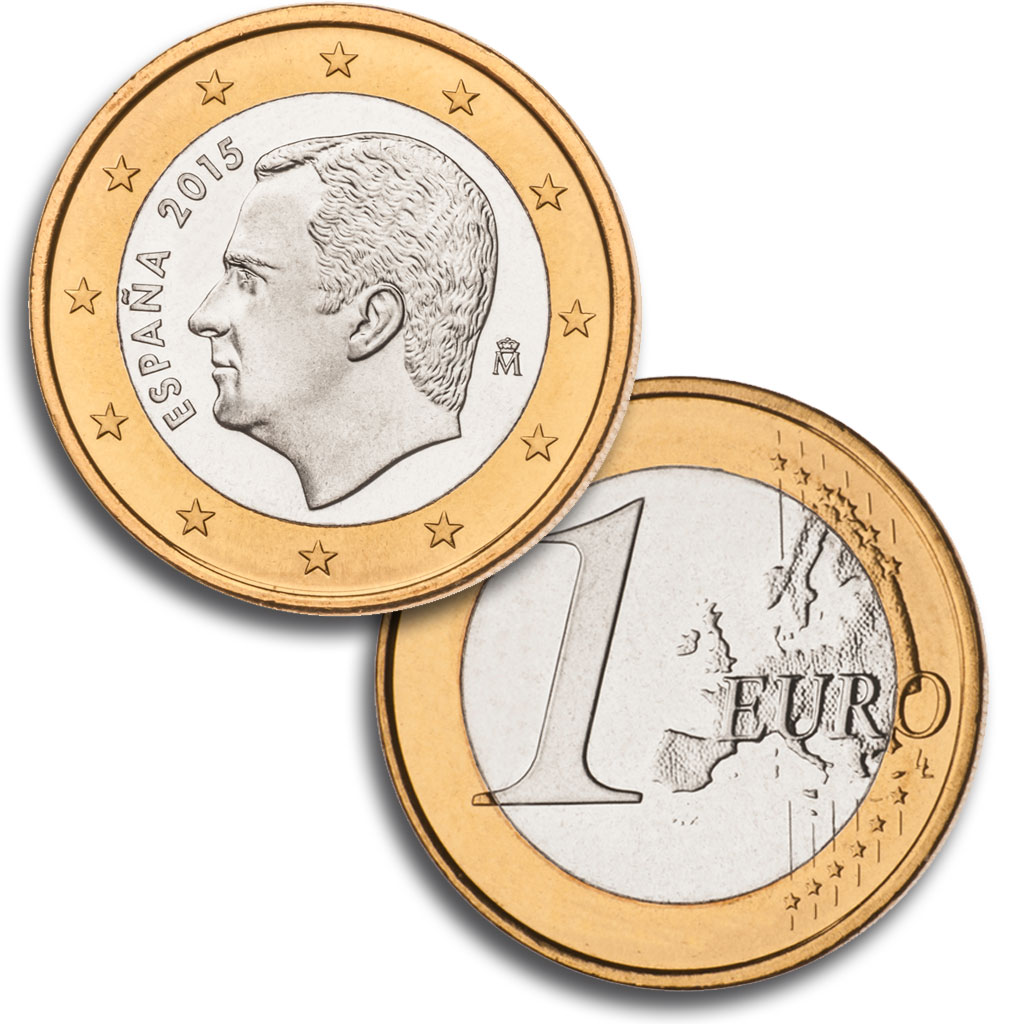
\includegraphics[width=0.7\textwidth]{img-04/monedes}
\end{minipage}
	

\begin{longtable}{|p{0.7in}|p{0.2in}|p{0.2in}|p{0.2in}|p{0.2in}|p{0.2in}|p{0.2in}|p{0.2in}|p{0.2in}|p{0.2in}|p{0.2in}|p{0.2in}|p{0.2in}|p{0.2in}|p{0.2in}|} \hline 
N. Tirades & 10 & 20 & 30 & 40 & 50 & 60 & 70 & 80 & 90 & 100 & 110 & 120 & 130 & 140 \\ \hline 
N. Cares &  &  &  &  &  &  &  &  &  &  &  &  &  &  \\ \hline 
Freq.\newline relativa &  &  &  &  &  &  &  &  &  &  &  &  &  &  \\ \hline 
\end{longtable}
  En la segona fila de la taula, anirem acumulant el nombre de cares que han anat sortint a cada grup. En la tercera fila, calcularem la freqüència relativa, és a dir, el nombre de cares dividit pel nombre de tirades. Amb aquests resultats contesta:
\begin{tasks} 
\task Quina és la probabilitat experimental d'obtenir cara? I d'obtenir creu?
\task Són equiprobables els successos treure cara i treure creu? Per què?
\end{tasks}

\answers{\href{https://piworld.es/\#!/home/activity/71/0}{Simulació}:\par
	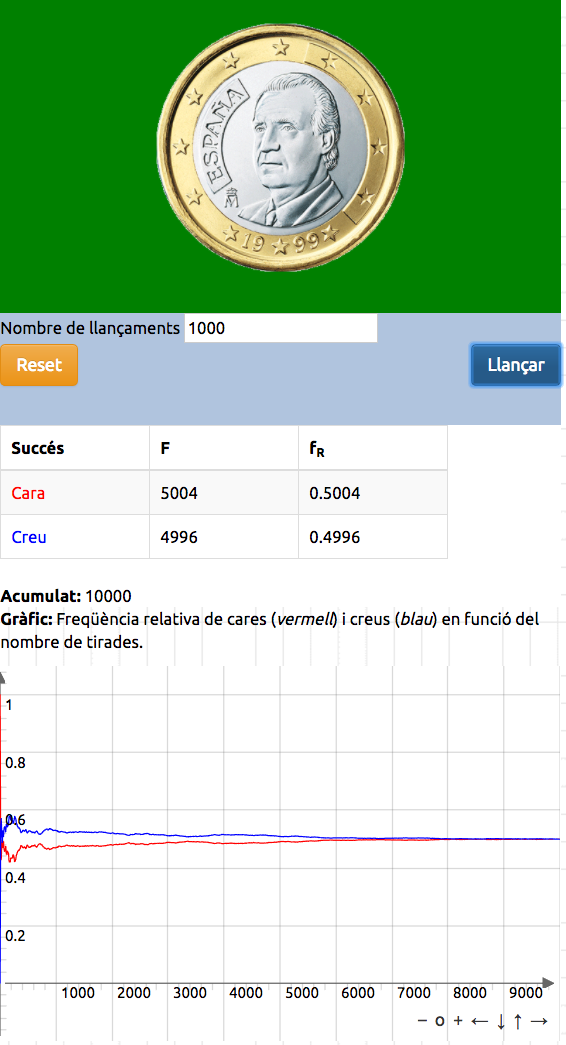
\includegraphics[width=0.4\textwidth]{img-sol/t4-sim-monedes} \par
\begin{tasks} \task Pel nombre més alt de tirades, cerca la freqüència relativa. Aquesta és la millor aproximació a la probabilitat d'obtenir cara. La probabilitat de treure creu és $P(X)=1-P(C)$ \task Sí. Són equiprobables. Perquè la moneda és simètrica i no està trucada.\end{tasks}}

\pagebreak
 
 \mbox{}
\vspace*{-2.5cm}
\exer \simbolsearch \begin{minipage}[t]{0.7\textwidth}  \textit{\bf Experiment llançament de xinxetes}. Agafa una xinxeta i fixeu-vos que pot caure de dues formes: punxa per amunt o de costat. Ara llança la xinxeta 10 vegades i compta quantes han sortit punxa per amunt. Tot seguit, el professor anirà demanant a cada grup quins han estat els resultats i els apuntarem en aquesta taula
	\end{minipage}
\begin{minipage}{0.3\textwidth}
\vspace{2cm}
\centering
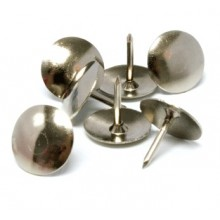
\includegraphics[width=0.8\textwidth]{img-04/xinxetes}
\end{minipage}

\begin{longtable}{|p{0.7in}|p{0.2in}|p{0.2in}|p{0.2in}|p{0.2in}|p{0.2in}|p{0.2in}|p{0.2in}|p{0.2in}|p{0.2in}|p{0.2in}|p{0.2in}|p{0.2in}|p{0.2in}|p{0.2in}|} \hline 
	N. Tirades & 10 & 20 & 30 & 40 & 50 & 60 & 70 & 80 & 90 & 100 & 110 & 120 & 130 & 140 \\ \hline 
	N. Amunt &  &  &  &  &  &  &  &  &  &  &  &  &  &  \\ \hline 
	Freq.\newline relativa &  &  &  &  &  &  &  &  &  &  &  &  &  &  \\ \hline 
\end{longtable}

En la segona fila de la taula, anirem acumulant el nombre de pics que cau la punxa per amunt. En la tercera fila, calcularem la freqüència relativa, és a dir, el nombre de punxes per amunt dividit pel nombre de tirades. Amb aquests resultats contesta:

\begin{tasks}
\task Quina és la probabilitat experimental de caure punxa per amunt? I  de caure de costat?
\task Són equiprobables els dos successos? Per què?
\end{tasks}

\answers[cols=1]{[Pel nombre més alt de tirades, cerca la freqüència relativa. Aquesta és la millor aproximació a la probabilitat de caure per amunt. La probabilitat de caure de costat és $P(costat)=1-P(amunt)$, No són equiprobables. Perquè la xinxeta pesa més d'una banda que de l'altre. Les dues bandes no són  simètriques.]}
\vso
 

\exer \mental En una bossa tenim 10 boles vermelles numerades de l'1 al 10. Es fan els dos experiments següents: 

 \quad EXPERIMENT A: Es treu una bola de la bossa i es mira el seu color.

 \quad EXPERIMENT B: Es treu una bola de la bossa i es mira el seu nombre.

 Quin d'aquests experiments no és un experiment aleatori? Per què?

 Pel cas que sigui un experiment aleatori, descriu el seu espai mostral.
\answers{L'experiment A és determinista perquè segur que surt bola vermella. L'experiment B és aleatori perquè no sabem el nombre que sortirà abans de fer l'experiment. L'espai mostral és E=\{1, 2, 3, 4, 5, 6, 7, 8, 9, 10\}}
\end{mylist}


  
\section{Probabilitats simples (Regla de Laplace)}

\begin{theorybox}
\video[ytid=hpag1\_CTp4k]{156}{Probabilitat: Regla de Laplace}  

                 Si tots els possibles resultats d'un experiment aleatori tenen la mateixa probabilitat (són \textbf{equiprobables}), podem aplicar la \textbf{regla de Laplace}:
\[P\left(S\right)=\frac{Nombre\ de\ casos\ favorables\ a\ S}{Nombre\ de\ casos\ totals}\] 
    \vspace{0.5cm}
\end{theorybox}
 
\pagebreak
 \begin{mylist}

\exer \spen  Troba la probabilitat d'obtenir un 2 i la probabilitat d'obtenir un 5, en llançar un dau correcte en cada un d'aquests casos:

\begin{longtable}{p{1.5in}p{1.2in}p{1.2in}} 
	\centering 
a) Dau cúbic (6 cares)\newline \includegraphics*[bb=0 0 0.66in 0.70in, width=0.66in, height=0.70in, keepaspectratio=false]{img-04/image3.png} & b) Dau tetraèdric (4 cares)\newline \includegraphics*[bb=0 0 0.73in 0.74in, width=0.73in, height=0.74in, keepaspectratio=false]{img-04/image4.png} & c) Dau octaèdric (8 cares)\newline \includegraphics*[bb=0 0 1.13in 0.89in, width=0.78in, height=0.76in, keepaspectratio=false, trim=0.31in 0.04in 0.04in 0.09in]{img-04/image5.png} \\ [0.5cm] \quad P(2) = ........ & \quad P(2) =......... & \quad P(2)=.......... \\  [0.2cm] \quad P(5) = ........ & \quad P(5) =......... & \quad P(5).......... \\
\end{longtable}

\answers{[$P(2)=\frac{1}{6}$; $P(5)=\frac{1}{6}$,  $P(2)=\frac{1}{4}$; $P(5)=0$,  $P(2)=\frac{1}{8}$; $P(5)=\frac{1}{8}$]}


  \exer \spen En una bossa hi ha 6 boles vermelles, 4 de blaves, 7 de verdes, 2 de grogues i una de negra. En treim una a l'atzar, calcula la probabilitat de que
\begin{tasks}(2)
	\task  Sigui blava.    
	\task  No sigui negra.
	\task  Sigui vermella o verda.   
	\task  No sigui groga ni negra.
\end{tasks}
\answers{[$\frac{4}{20}$, $\frac{19}{20}$, $\frac{13}{20}$, $\frac{17}{20}$]}
 

\exer  Raona de quina de les bosses següents és més probable treure una bola negra:
\begin{center}
 \includegraphics*[  width=2.91in ]{img-04/image6.png}
\end{center}
\answers{De la bossa I. Perquè P(I)=$\frac{2}{3}=0.666...$, P(II)=$\frac{4}{7}=0.571$ i P(III)=$\frac{3}{5}=0.6$}

\exer \spen Llançam un dau regular. Calcula les probabilitats que el resultat sigui:
\begin{tasks}(2)
	\task    Múltiple de  3   
	\task  Múltiple de 2
	\task    Major que 1    
	\task  Menor que 5
	\task    Menor que 1   
	\task   Potència de 2
\end{tasks}
 \answers{[$\frac{2}{6}$, $\frac{3}{6}$, $\frac{5}{6}$, $\frac{4}{6}$, 0, $\frac{3}{6}$]}

\exer \spen  Extreim una carta d'una baralla espanyola de 40 naips. Calcula la probabilitat que:
\begin{tasks} 
\task  La carta sigui de BASTOS
\task  La carta NO sigui ni AS ni FIGURA
\task  La carta sigui menor que 6
\task  La carta sigui d'OROS o FIGURA
\end{tasks}
\answers{[$\frac{10}{40}$, $\frac{24}{40}$, $\frac{20}{40}$, $\frac{19}{40}$]}
 
 \exer  Extreim una carta d'una baralla espanyola de 40 naips. Troba la probabilitat que:
 \begin{tasks}(2)
 	\task  Sigui un CINC    
 	\task  No sigui un CAVALL
 	\task     Sigui d'OROS o de COPES   
 	\task  No sigui d'ESPASES
 \end{tasks}
 \answers{[$\frac{4}{40}$, $\frac{36}{40}$, $\frac{20}{40}$, $\frac{30}{40}$]}
\newpage

 \exer[1] En un llibre de 120 pàgines, hem comptat el nombre d'errades en cadascuna de les pàgines. Els resultats han estat: 

\begin{longtable}{|p{2.3in}|p{1.4in}|} \hline 
\textbf{Nº d'errades} & \textbf{Nº de pàgines} \\ \hline 
0 & 58 \\ \hline 
1 & 42 \\ \hline 
2 & 16 \\ \hline 
3 & 3 \\ \hline 
4 & 1 \\ \hline 
\end{longtable}

Si triam una pàgina a l'atzar:
\begin{tasks} 
	\task  Quina és la probabilitat que no tingui cap errada?
	\task  Quina és la probabilitat que tingui exactament dues errades?
	\task  I la probabilitat que tingui alguna errada? I que tingui més de tres?
\end{tasks}
\answers[cols=3]{[$\dfrac{58}{120}$, $\dfrac{16}{120}$, $\dfrac{62}{120}$  i $\dfrac{1}{120}$ ]}
 

  

\exer  D'aquesta urna extreim una bola i n'observam el nombre i el color. Calcula les probabilitats dels successos següents:
\begin{center}
	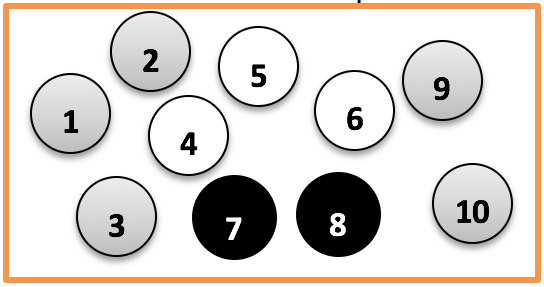
\includegraphics[width=5cm]{img-04/image11}
\end{center}
\begin{tasks} 
	\task  Obtenir una bola blanca amb un nombre parell
	\task  Obtenir bola negra amb nombre parell
	\task  Obtenir bola grisa o negre
	\task  Obtenir una bola amb nombre més gran que 7
\end{tasks}

\answers{[$\frac{1}{10}$, $\frac{1}{10}$, $\frac{7}{10}$, $\frac{3}{10}$]} 

\exer  D'una bossa amb 7 boles vermelles, 5 de verdes, 3 de grogues, 11 de negres i 3 de blaves, en treim una a l'atzar. Quina és la probabilitat que 
\begin{tasks} 
	\task    Sigui vermella?    
	\task  No sigui negra?
\end{tasks}
\answers{[$\frac{7}{29}\approx 0.24$, $\frac{18}{29}\approx 0.62$]}

\end{mylist}


\section{Probabilitat composta}

\begin{theorybox}
 \videonw[ytid=zLGB4hZyNeI]{157}{Probabilitat successos composts independents}

                      Si A i B són successos independents, es compleix que \textbf{P(A i B) = P(A)·P(B)                           }
                      
                      \normalfont{\textit{Per exemple}}: Treure dues cartes\textbf{ amb reemplaçament} (les tornam a ficar).

\videonw[ytid=3v1p6nXos\_s]{159}{Probabilitat successos composts dependents} 

                     \normalfont{\textit{Per exemple}}: Treure dues cartes \textbf{sense reemplaçament} (no les tornam a ficar). Utilitzam la tècnica de    \textbf{ diagrames d'arbre}.
\end{theorybox}

\subsection{Successos independents}

\begin{resolt}[E]{
	
Llançam un dau i treim una carta d'una baralla espanyola de 40 cartes. Quina és la probabilitat d'obtenir múltiple de 3 al dau i rei a la carta?
	
}
	\textbf{Compost independent}

	\[P(\text{\boxed{3,6} i \boxed{rei}})= P(\text{\boxed{3,6}}) \cdot P(\text{\boxed{rei}}) = \frac{2}{6}\cdot \frac{4}{40}=\frac{1}{30} \]
	
\end{resolt}

\begin{mylist}
	

\exer Llançam un dau i una moneda. Calcula les probabilitats:
\begin{tasks}(2)
	\task  Treure un 6 i cara     
	\task  Treure parell i creu.
\end{tasks}
\answers{[$\frac{1}{6}\cdot \frac{1}{2}=\frac{1}{12}$, $\frac{3}{6}\cdot \frac{1}{2}=\frac{1}{4}$]}


\exer  Es considera l'experiment aleatori de tirar un dau dues vegades. Calcula les probabilitats següents:  
\begin{tasks}(2)
	\task  Treure algun 1.     
	\task  La suma dels dígits és 8. 
	\task  No treure cap 2.    
	\task  Treure algun 1 o bé no treure cap 2.
\end{tasks}
 \answers{Si $A$=\{1,2,3,4,5,6\}, cal calcular el producte cartesià $A\times A$.\par
\begin{tasks}(2) \task $\frac{11}{36}$ \task  $\frac{5}{36}$ \task  $\frac{25}{36}$ \task  $\frac{31}{36}$\end{tasks}}
  
\exer[1]  Es considera l'experiment aleatori de tirar una moneda tres vegades. Calcula les probabilitats següents:  
\begin{tasks}(2) 
	\task  Treure cara en la primera tirada.   
	\task  Treure cara en la segona tirada.
	\task  Treure cara en la tercera tirada.  
	\task  Treure alguna cara. 
	\task  No treure cap cara.     
	\task  Treure tres cares. 
\end{tasks}
\answers[cols=3]{[$\frac{1}{2}$, $\frac{1}{2}$, $\frac{1}{2}$, $1-\dfrac{1}{8}=\dfrac{7}{8}$, $\frac{1}{8}$, $\frac{1}{8}$]}

 \exer[1]  Es considera l'experiment aleatori treure dues cartes de la baralla espanyola amb reemplaçament. Calcula la probabilitat de:  
 \begin{tasks}(2)
 	\task  Treure algun rei.        
 	\task  Obtenir almenys un basto. 
 	\task  No obtenir cap basto.       
 	\task  No obtenir el rei de bastos. 
 	\task  Treure figura: sota, cavall, rei o as.     
 	\task  No treure cap figura.
 \end{tasks}
 \answers[cols=3]{[0.19, 0.44, 0.56, 0.95, 0.65, 0.35]}

\newpage

\exer  En llançar quatre monedes a l'aire,  
\begin{tasks}
	\task  Quina és la probabilitat que les quatre siguin cares?
	\task  Quina és la probabilitat d'obtenir com a màxim tres cares? 
	\task  Quina és la probabilitat de tenir exactament 3 cares?
\end{tasks}
\answers[cols=1]{[$\left(\frac{1}{2}\right)^4= \frac{1}{16}$, $1-P(CCCC)=1-\frac{1}{16}=\frac{15}{16}$, $4 P(XCCC)=4\left(\frac{1}{2}\right)^4=\frac{1}{4}$]}
  

 \exer[1] \label{list:boles} En una urna hi ha 6 boles blanques i 14 boles negres. Es treuen dues boles amb reemplaçament. Determina la probabilitat que: 
\begin{tasks}(2)
	\task  Les dues siguin negres.  
	\task  Hi hagi almenys una negra.  
	\task  Cap sigui negra.
\end{tasks}
\answers[cols=3]{[$\dfrac{49}{100}$, $\dfrac{91}{100}$, $\dfrac{9}{100}$]}

\subsection{Successos dependents. Diagrames d'arbre}

\begin{resolt}[E]{
	 Dos tiradors al plat tenen unes marques ja conegudes. El primer encerta amb una probabilitat de 0,7 i el segon de 0,4. Es llança un plat i tots dos disparen. Expressa mitjançant un diagrama d'arbre i les diferents possibilitats: 
	 \vspace{0.5cm}
	 
	 \begin{tasks}
	 	\task  Calcula la probabilitat que cap encerti.
	 	\task  Calcula la probabilitat que els dos encertin.
	 	\task  Quina probabilitat hi ha que un dels tiradors doni en el plat?
	 \end{tasks}
}
	Per resoldre aquest problema, utilitzam la tècnica del diagrama d'arbre 
	
	Recorda: Les probabilitats d'un camí de l'arbre es multipliquen. Diferents camins es sumen:
	
	\begin{center}
	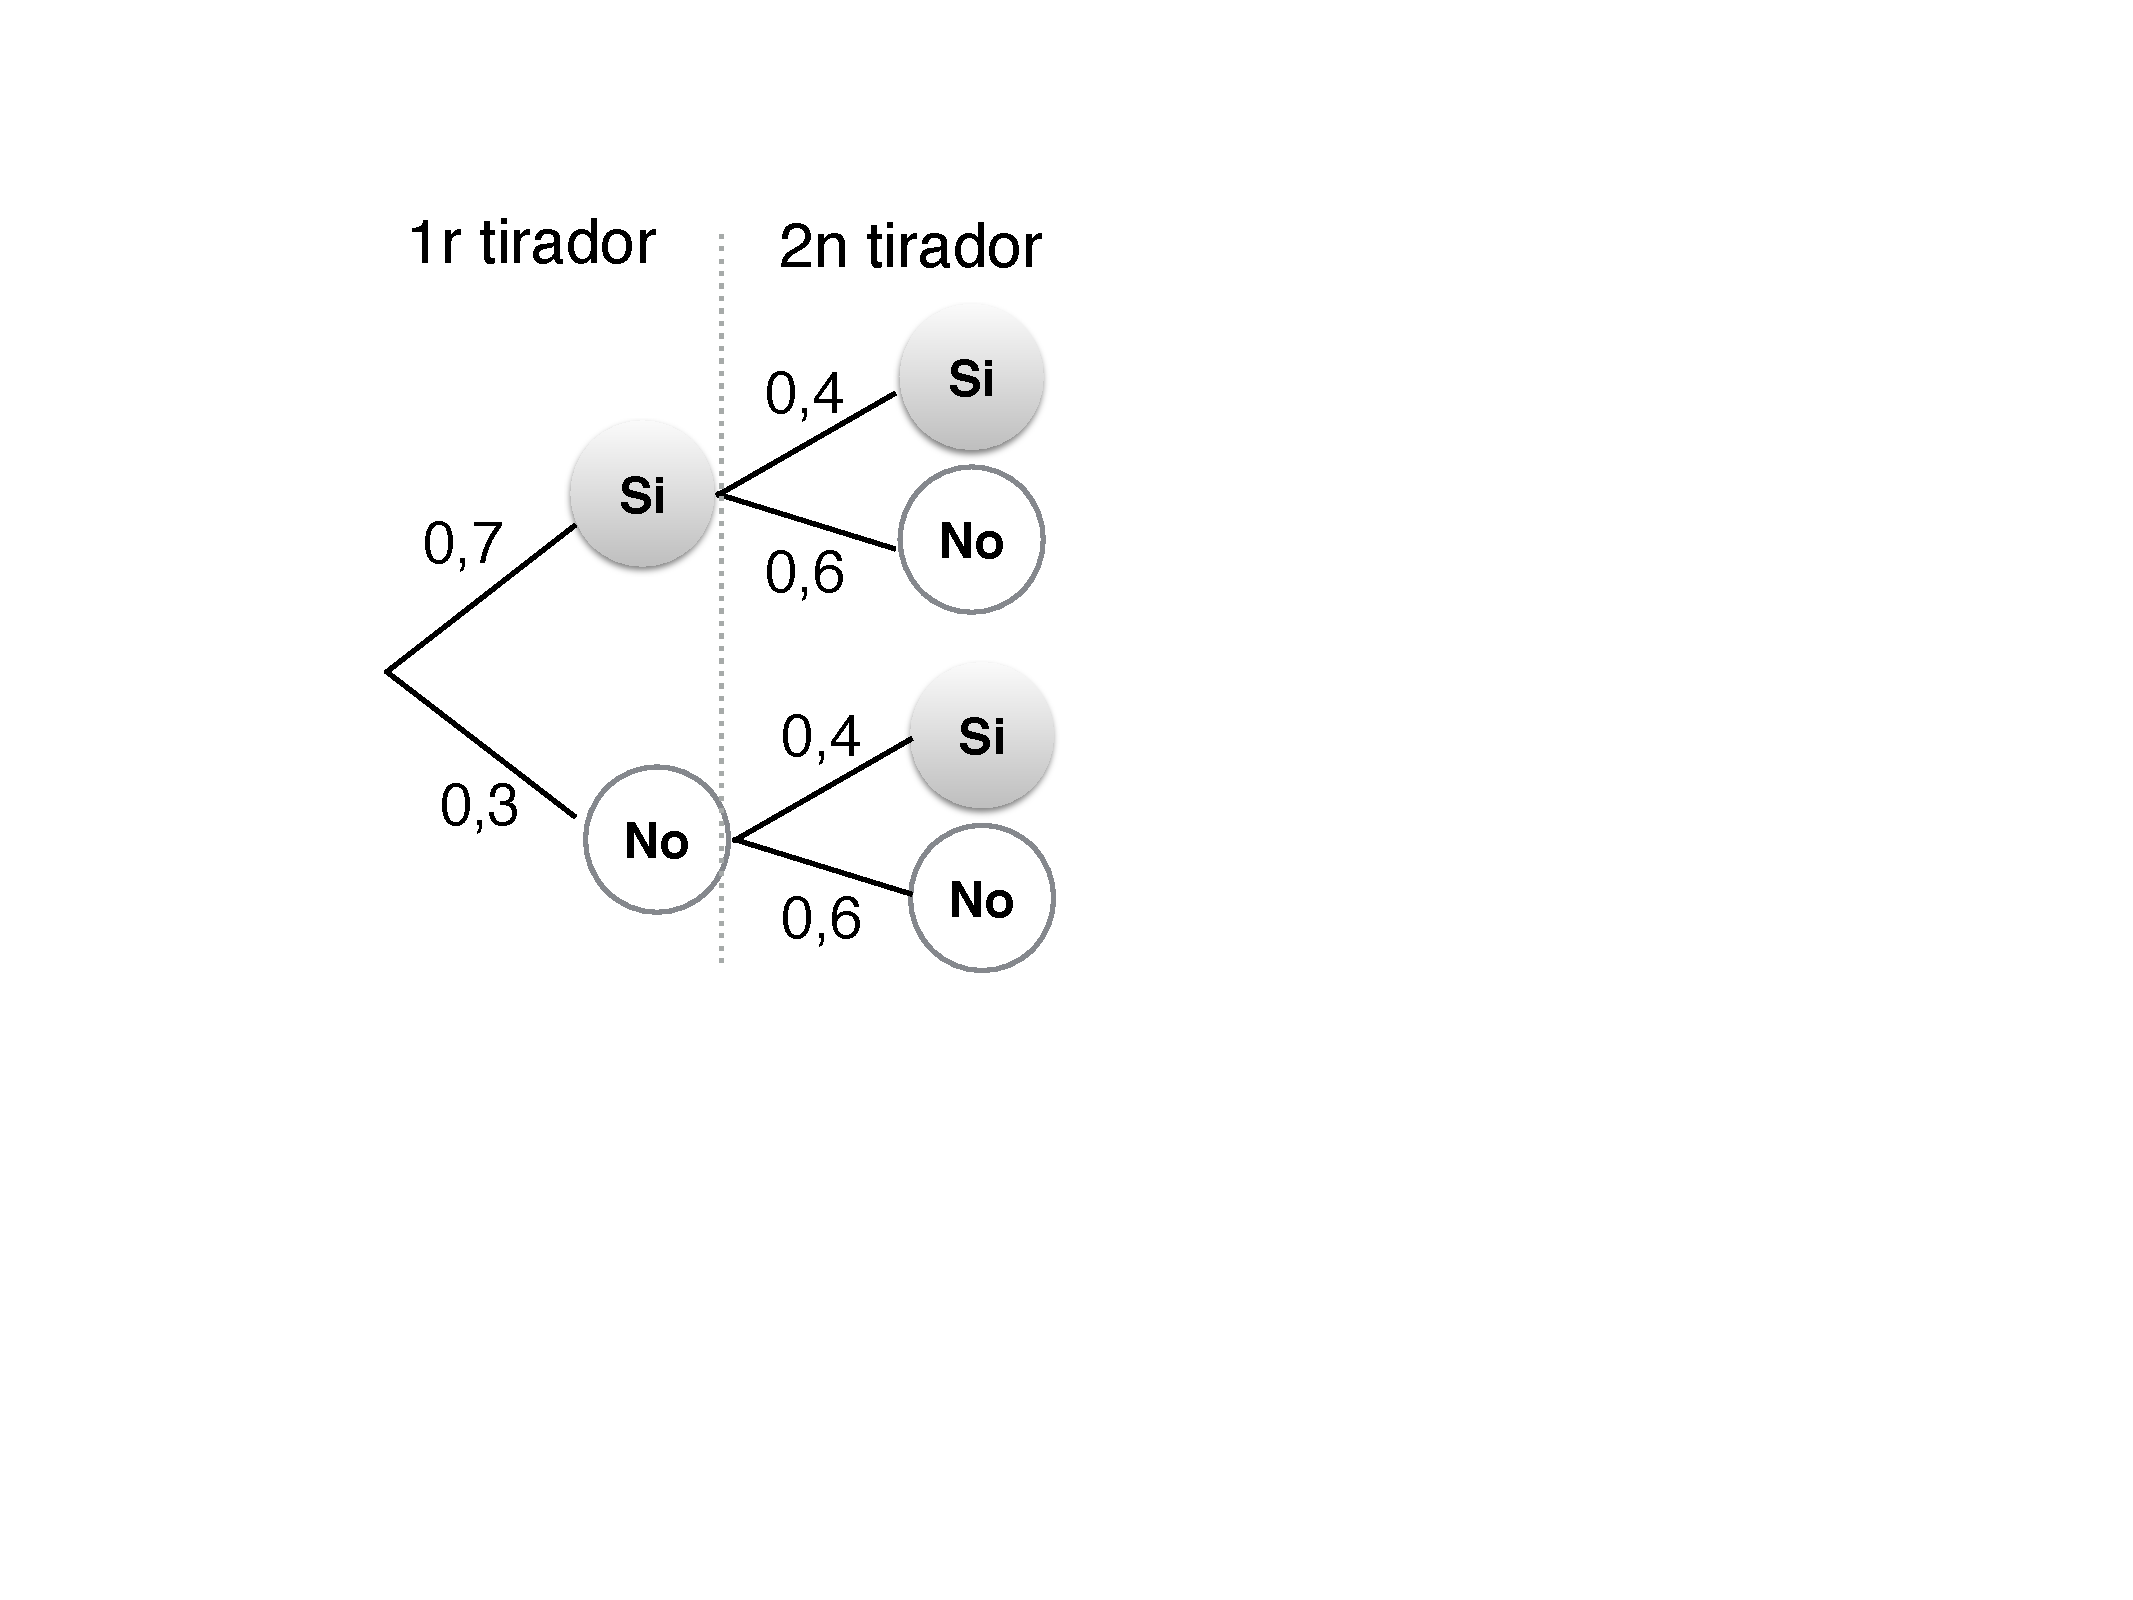
\includegraphics[width=4.5cm]{img-04/arbre}
	\end{center}
	
	a) $P(No-No)=0,3 \cdot 0,6 = 0,18$
	
	b) $P(Si-Si)=0,7 \cdot 0,4 = 0,28$
	
	c) $P(Un)= P(No-Si)+P(Si-No) = 0,3 \cdot 0,4 + 0,7\cdot 0,6 = 0,54$
	
\end{resolt}
 
\exer[1]  En una urna hi ha 6 boles blanques i 14 boles negres. Es treuen dues boles sense reemplaçament. Determina la probabilitat que: 
\begin{tasks}
	\task  Les dues siguin negres. 
	\task  Hi hagi almenys una negra.
	\task  Cap sigui negra.
	\task  Compara els resultats amb els de l'activitat \ref{list:boles}.
\end{tasks}
\answers[cols=3]{[$\dfrac{91}{100}$, $\dfrac{35}{38}$, $\dfrac{3}{38}$]}

 \exer Amb una baralla espanyola es fa l'experiment de treure tres cartes, amb reemplaçament, quina és la probabilitat de treure tres reis? I si l'experiment es fa sense reemplaçament, quin és ara la probabilitat de tenir 3 reis? 
 
 \answers[cols=1]{[Amb reemplaçament $P(RRR)=\frac{4}{40}\cdot \frac{4}{40} \cdot \frac{4}{40} =\frac{1}{1000}=0.001$,
 	Sense reemplaçament $P(RRR)=\frac{4}{40}\cdot \frac{3}{39} \cdot \frac{2}{38} =\frac{1}{2470}=0.0004$]}
 
 \newpage
\exer  Es llança una moneda fins que aparegui cara dues vegades seguides. 

\begin{tasks}
	\task  Calcula la probabilitat que l'experiment acabi en el segon llançament.
	\task  Calcula la probabilitat que acabi en el tercer llançament.
\end{tasks}
\answers[cols=1]{[$P(CC)=\frac{1}{4}$, $P(XCC)=\frac{1}{8}$]}
 

\exer[1]  En el llançament de naus espacials s'han instal·lat tres dispositius de seguretat A, B i C. Si falla A se posa automàticament en marxa el dispositiu B, i si falla aquest, s'engega C. Se sap que la probabilitat que falli A és 0,1, la probabilitat que B funcioni és 0,98 i la probabilitat que falli C és 0,05. Calcula la probabilitat que tot funcioni bé. 
\answers{$P=0.9999$}
  

 \exer Es fa un estudi sobre els incendis forestals d'una zona i es comprova que el 40 \% són intencionats, el 50 \% es deuen a negligències i el 10 \% a causes naturals. S'han produït tres incendis,  quina és la probabilitat que

 
 \begin{minipage}{0.8\textwidth}
	\begin{tasks}
		\task  almenys un hagi estat intencionat?
		\task  els tres incendis es deguin a causes naturals.
		\task  cap incendi sigui per negligències.
	\end{tasks}
\end{minipage}
\begin{minipage}{0.15\textwidth}
	\centering
	
\includegraphics[width=0.7\textwidth]{img-04/incendi}
\end{minipage}

\answers{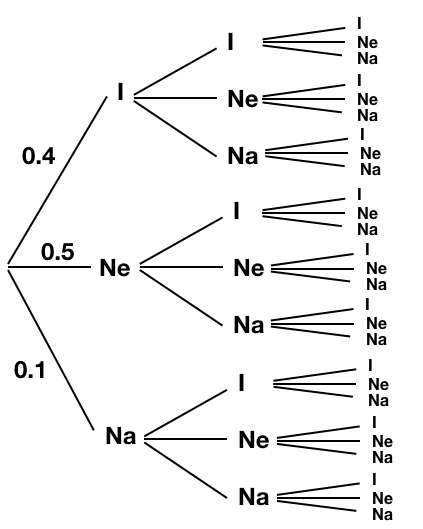
\includegraphics[width=0.35\textwidth]{img-sol/t4-42} \par
\begin{tasks} \task $P=1 – P(cap intencionat) = 1 – 0.63 = 0.784$ \task $P=(0.1)^3=0.001$, $P=0.5^3=0.125$ \end{tasks}}

\exer  Es llança dues vegades un dau equilibrat amb sis cares. Trobar la probabilitat que la suma dels valors que apareixen en la cara superior sigui múltiple de tres. 
\answers{Fer el producte cartesià.\par S'obté $P=\frac{12}{36}=\frac{1}{3}$}
  

 \exer \hot Se sap que s'han eliminat diverses cartes d'una baralla espanyola que té quaranta. La  probabilitat d'extreure un as entre les que queden és 0,12, la probabilitat que surti una copa és 0,08 i la probabilitat que no sigui ni As ni copa és 0.84. 

 Calculau la probabilitat que la carta sigui l'as de copes. Es pot afirmar que entre les cartes que no s'han eliminat està l'as de copes?
\answers{\begin{tabular}{c|ccc}
		 & As & No As & \\  \hline
	Copa & 0.04 & 0.04 & 0.08 \\
	No copa & 0.08 & 0.84 & 0.92 \\
	  & 0.12 & 0.88 & 1 \\
\end{tabular}
\par
P(As copes)=0.04; No s'ha eliminat l'as de copes.}
 

\exer[1] Una persona despistada té vuit mitjons negres, sis blaus i quatre vermells, tots ells solts. Un dia amb molta pressa, tria dos mitjons a l'atzar. Trobau la probabilitat de:  

\begin{minipage}{0.65\textwidth}	
	\begin{tasks}
		\task  que els dos mitjons siguin negres. 
		\task  que els dos mitjons siguin del mateix color.
		\task  que  almenys un d'ells sigui vermell.
		\task  que un sigui negre i l'altre no.
	\end{tasks}
\end{minipage}
\begin{minipage}{0.29\textwidth}
	\centering
	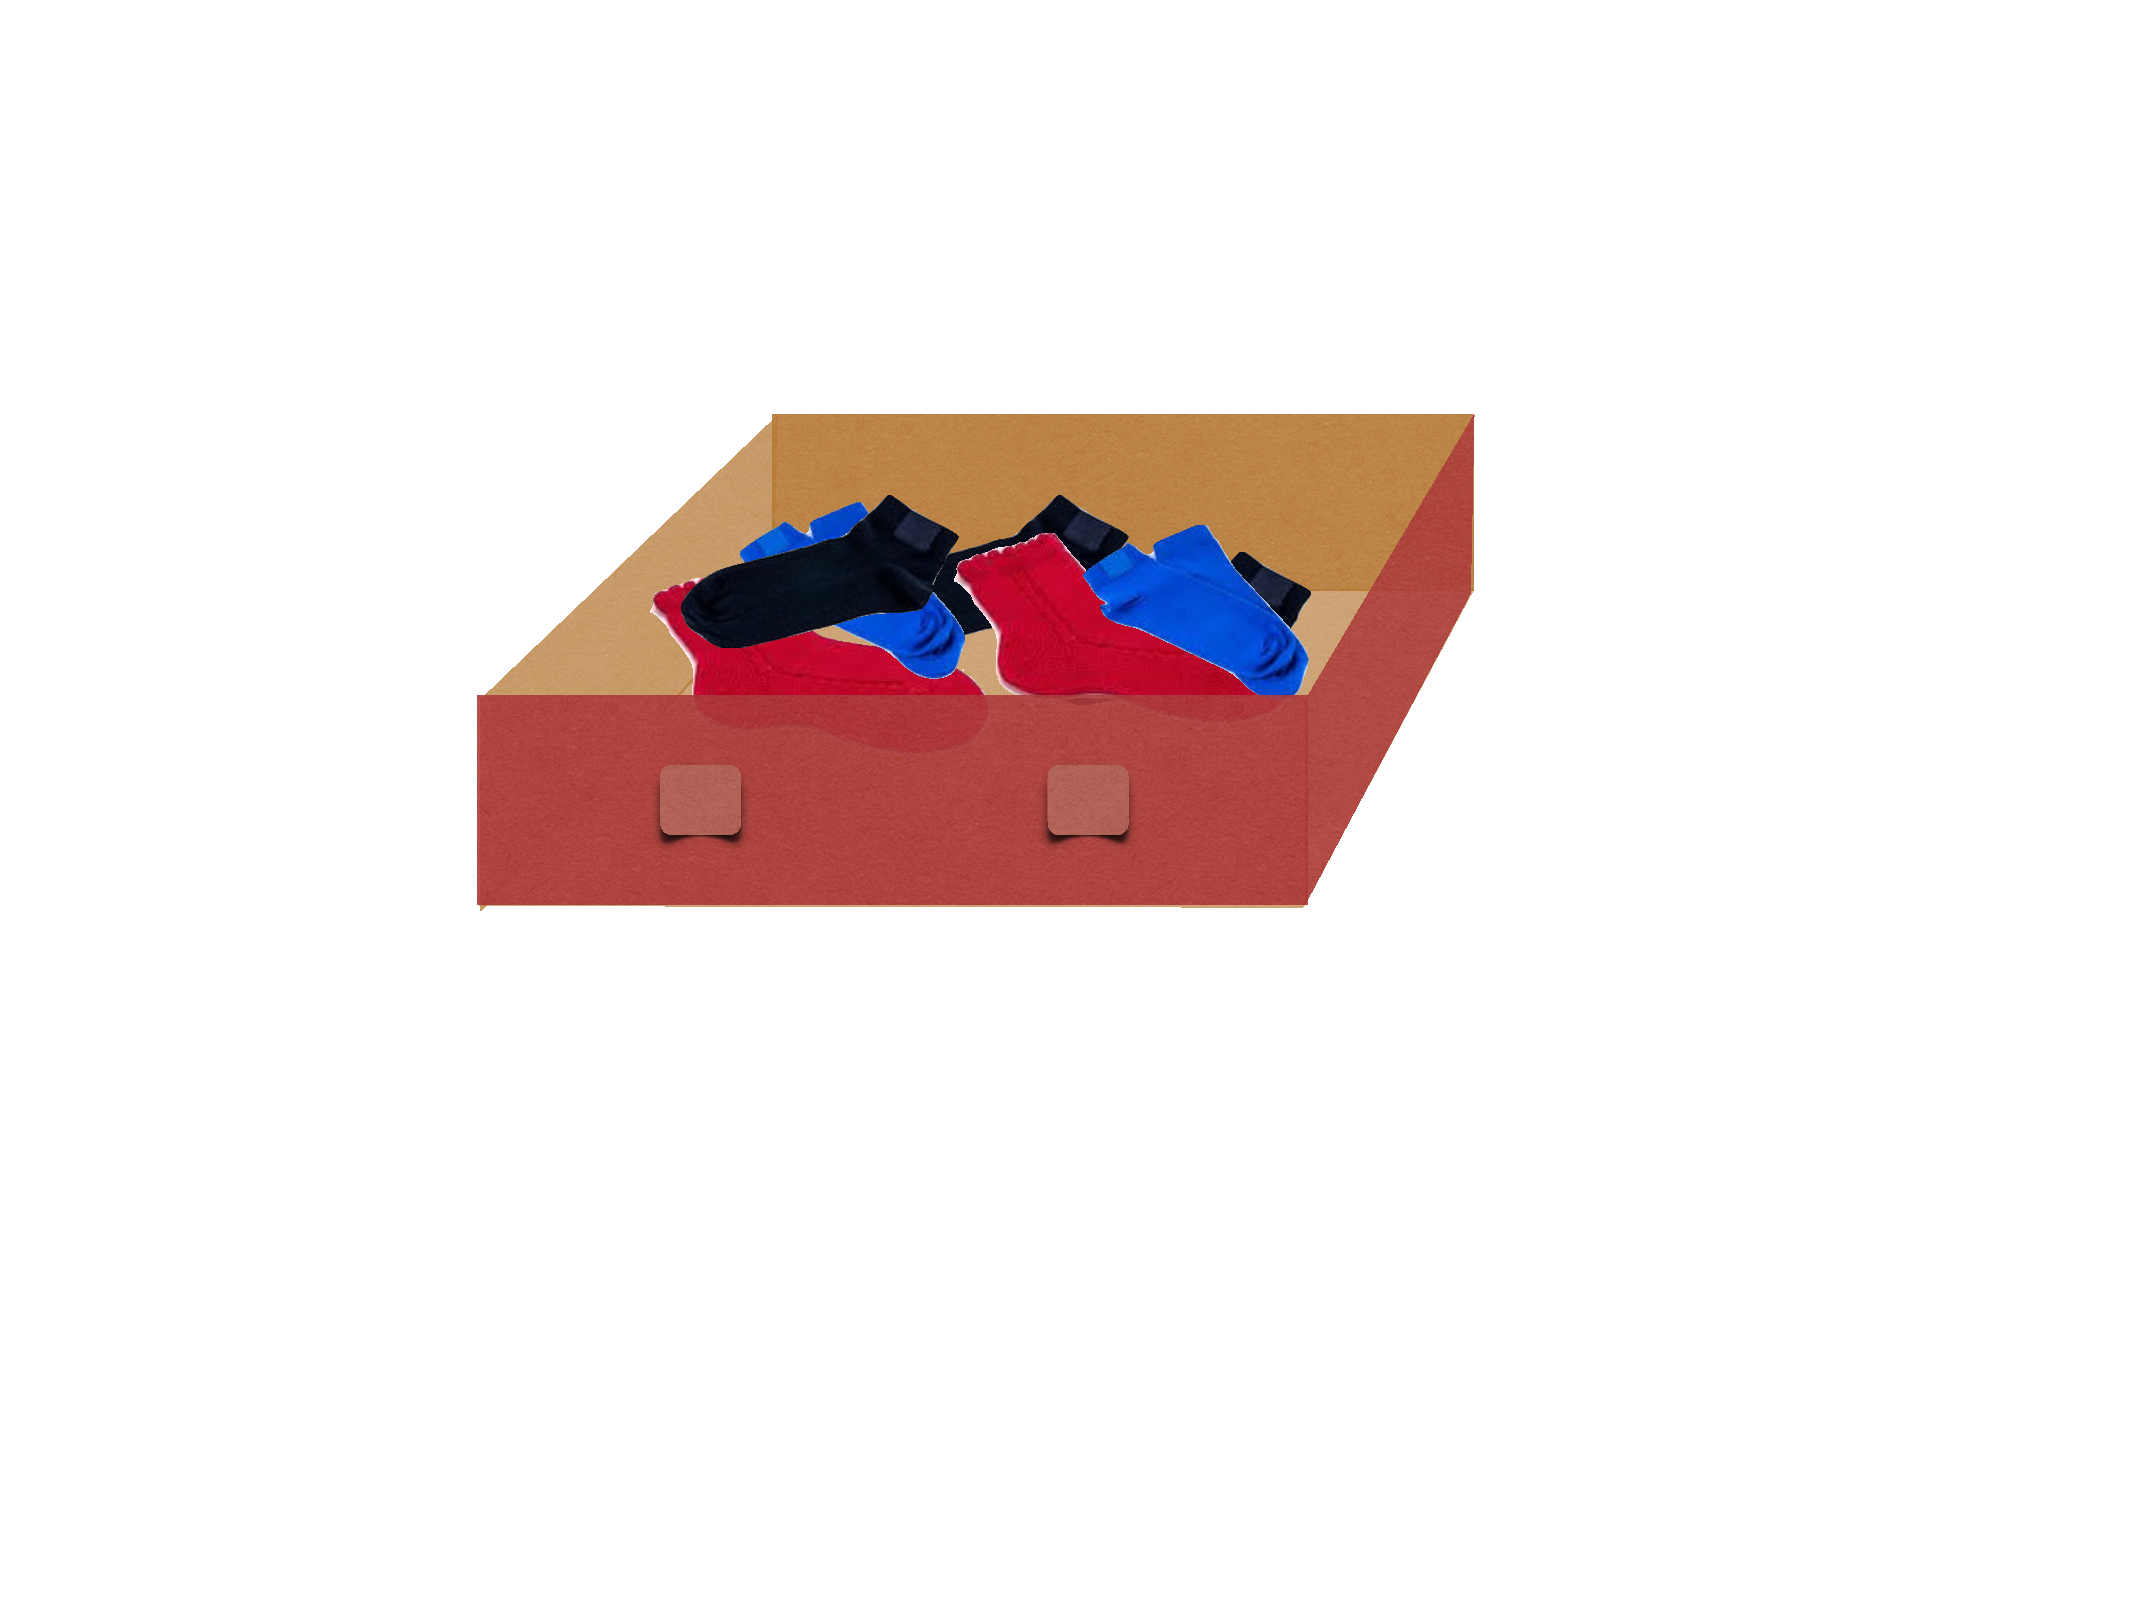
\includegraphics[width=0.94\textwidth]{img-04/calcetins}
\end{minipage}

\answers[cols=1]{[$\dfrac{28}{153}$, $\dfrac{49}{153}$, $\dfrac{62}{153}$, $\dfrac{80}{153}$]}
 

 \exer Tres persones viatgen en un cotxe. Si suposam que la probabilitat de néixer en un dia qualsevol de l'any és la mateixa i sabem que cap d'elles ha nascut en un any de traspàs, 
\begin{tasks}
	\task  trobau la probabilitat que només una d'elles celebri el seu aniversari aquest dia.
	\task  calculau la probabilitat que almenys dues compleixin anys aquest dia.
\end{tasks}
\answers[cols=1]{[$3\left(\dfrac{1}{365}\right)\left(\dfrac{364}{365}\right)^2 = 0,008174203184$, 
  $3 \left(\dfrac{1}{365}\right)^2 \left(\dfrac{364}{365}\right)+ \left(\dfrac{1}{365}\right)^3 = 0,000022456602$
 ]}
\end{mylist}

\pagebreak

\begin{autoaval}{51}
\begin{mylist}
 \exer[2] Es fa un estudi sobre el color que prefereixen els habitants d'un país per a un cotxe. La variable utilitzada és:
\begin{tasks}(4)
	\task  quantitativa  
	\task  qualitativa  
	\task  quantitativa discreta  
	\task  quantitativa contínua
\end{tasks}
\answers{\textbf{--10.}: Claus de l'autoavaluació: 1b;  2c; 3c; 4b; 5d; 6a; 7a; 8b; 9d; 10c}

\begin{comment}
 \exer En un histograma de freqüències relatives l'àrea de cada rectangle és: 
\begin{tasks}(4)
	\task  proporcional a l'àrea     
	\task  igual a la freqüència absoluta 
	\task  proporcional a la freqüència relativa   
	\task  proporcional a la freqüència acumulada 
\end{tasks}
\end{comment}

\exer En un equip de futbol de 11 jugadors, la mitjana de les edats és de 28 anys. A mitjan partit, l'arbrit expulsa a un jugador i ara la mitjana és de 27 anys. Quina és l'edat d'aquest jugador?  
\begin{tasks}(4)
	\task  27  
	\task  28  
	\task  38  
	\task  No es pot saber
\end{tasks}

 \exer Anna ha obtingut en Matemàtiques les següents notes: 7, 8, 5, 10, 8, 10, 9 i 7. La seva nota mitjana és de:
\begin{tasks}(4)
	\task  7,6  
	\task  8,2  
	\task  8  
	\task  9
\end{tasks}

 \exer En les notes anteriors d'Anna la desviació típica és:
\begin{tasks}(4)
	\task 0,89 
	\task 1,58  
	\task 2,50 
	\task 7,64
\end{tasks}

 \exer En les notes anteriors d'Anna la moda és:
\begin{tasks}(4)
	\task  10  
	\task  8  
	\task  7 
	\task  7, 8 i 10
\end{tasks}

 \exer L'espai mostral de successos elementals equiprobables de l'experiment ``tirar dues monedes i comptar el nombre de cares'' és:
\begin{tasks}(4)
	\task  $\{2C, 1C, 0C\}$  
	\task  $\{CC, CX, XC, XX\}$  
	\task  $\{XX, XC, CC\}$  
	\task  $\{CC, CX, XC, CC\}$
\end{tasks}

\exer Tirem dos daus i sumem els punts de les cares superiors. La probabilitat que la suma sigui 7 és:
\begin{tasks}(4)
	\task  1/6  
	\task  7/36  
	\task  5/36  
	\task  3/36
\end{tasks}

 \exer En treure una carta d'una baralla espanyola (de 40 cartes), la probabilitat que sigui un or o bé un rei és:
\begin{tasks}(4)
	\task  14/40  
	\task  13/40  
	\task  12/40  
	\task  15/40
\end{tasks}

 \exer En una bossa hi ha 7 boles vermelles, 2 negres i 1 bola blanca. Es treuen 2 boles sense reemplaçament. La probabilitat que les dues siguin vermelles és:
\begin{tasks}(4)
	\task  49/100  
	\task  42/100  
	\task  49/90 
	\task  7/15
\end{tasks}

 \exer Tirem tres monedes a l'aire. La probabilitat que les tres en caure siguin cares és:
\begin{tasks}(4)
	\task  1/5 
	\task  1/7 
	\task  1/8  
	\task  1/6
\end{tasks}
\end{mylist}
\end{autoaval}

\newpage
\resum
\begin{center}
\renewcommand{\arraystretch}{1}
\begin{longtable}{|p{0.19\textwidth}|p{0.38\textwidth}|p{0.36\textwidth}|} \hline 
 \rowcolor{lightgray} &  & \textit{Exemples} \\ \hline 
\cellcolor{lightgray} \textbf{Població} & Col·lectiu sobre el qual es  fa l'estudi & \textit{Estudiants de totes les Balears} \\ \hline 
\cellcolor{lightgray} \textbf{Mostra} & Subconjunt de la població que permeti obtenir característiques de la població completa. & \textit{Alumnes es 3r d'ESO seleccionats} \\ \hline 
\cellcolor{lightgray} \textbf{Individu} & Cadascun dels elements de la població o mostra & \textit{Joan Font} \\ \hline 
\cellcolor{lightgray} \textbf{Variables} 
	
\textbf{estadístiques} & Quantitativa discreta \newline Quantitativa contínua\newline Qualitativa & Nombre de peu que calça\newline Alçada\newline Esport que practica \\ \hline 
\cellcolor{lightgray} \textbf{Gràfics} 
	
\textbf{estadístics } &  Diagrama de barres\newline Histograma de freqüències\newline Polígon de freqüències\newline Diagrama de sectors & \  \\ \hline 
\cellcolor{lightgray} \textbf{Mitjana} & \textit{  }  $\overline{x}=\frac{\sum{f_i\textrm{·}x_i}}{N}\mathrm{=}\frac{x_{\mathrm{1}}\mathrm{\ }\mathrm{+\ }x_{\mathrm{2}}\mathrm{\ }\mathrm{+\ \dots +\ }x_N}{N}$ & Amb les dades: 8, 2, 5, 10 i 10\newline $\bar x$  = 35/5 = 7 \\ \hline 
\cellcolor{lightgray} \textbf{Moda} & És el valor més freqüent & \textit{Mo }= 10 \\ \hline 
\cellcolor{lightgray} \textbf{Mediana} & Queda per davall la meitat  & 4 $<$ 6 $<$ \textbf{8} $<$ 10 = 10.\textit{ Me =} 8. \\ \hline 
\cellcolor{lightgray} \textbf{Rang o }
	
\textbf{recorregut} & És la diferència entre la dada major i la dada menor.  & 10 -- 2 = 8 \\ \hline 
\cellcolor{lightgray} \textbf{Desviació }
	
\cellcolor{lightgray} \textbf{mitjana} & És la mitjana de les distàncies de les dades a la mitjana de les dades dels quals disposem.\newline \[DM = \frac{\sum |x_i - \bar x|}{N} \]  & 

 $\frac{\left|{\rm 8- 7}\right|{\rm +}  \left|{\rm 2- 7}\right| \cdots  {\rm +}\left|{\rm 10- 7}\right|}{{\rm 5}} = $  

$=\frac{1+5+2+3+3}{5} =\frac{14}{5}$\\ \hline 
\cellcolor{lightgray} \textbf{Variància} & És la mitjana dels quadrats de les distàncies de les dades a la mitjana: $Var=\frac{\sum{fx^2}}{N}-{\overline{x}}^2$ & ${\rm Var}=\frac{{\rm 1}+2{\rm 5}+{\rm 4}+{\rm 9}+{\rm 9}}{5} =\frac{47}{5} ={\rm 9},{\rm 4}$ \\ \hline 
\cellcolor{lightgray} \textbf{Desviació típica} & És l'arrel quadrada de la variància  $\sigma =\sqrt{Var}$ & Coeficient de variació (C.V.) $C.V. = \sigma / \bar x$  \\ \hline 
\cellcolor{lightgray} \textbf{Probabilitat} & Valor entre 0 i 1 que ens dóna una mesura del factible que sigui que es produeixi un determinat succés.  & $P(3) = 1/6$ en tirar un dau \\ \hline 
\cellcolor{lightgray} \textbf{Espai mostral} & El conjunt de tots els casos possibles  & $\{ 1, 2, 3, 4, 5, 6 \}$ \\ \hline 
\cellcolor{lightgray} \textbf{Succés} & Subconjunt de l'espai mostral & Treure parell: $\{ 2, 4, 6 \}$ \\ \hline 
\cellcolor{lightgray} \textbf{Llei de Laplace} & $P(S)=\frac{\text{N. casos favorables a S}}{\text{N. casos totals}} $ & \textit{P}(parell) = 3/6 = 1/2. \\ \hline 
\end{longtable}

\end{center}


 




 


 
 
\mychapter{Àlgebra: Polinomis}{Àlgebra: Polinomis}{ \centering
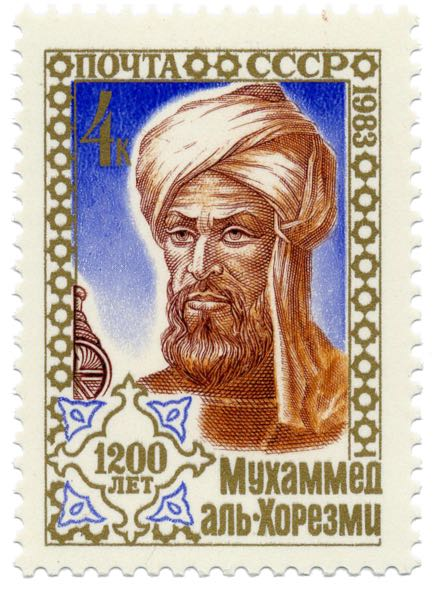
\includegraphics[height=4cm]{img-05/juarismi} \par \footnotesize Al Juarismi (segle IX d.C) \par Pare de l'àlgebra.}{chap:algebra}
 
\vspace*{\fill} 
 
\begin{iniaval}  
\textbf{Classifica en vertaderes o falses les següents expressions:}

\begin{center}
	
\def\arraystretch{4}
\begin{longtable}{|p{1.1in}|p{1.1in}|p{1.1in}|p{1.1in}|} \hline 
\cellcolor{red!50}$\boldsymbol{a}\boldsymbol{+}\boldsymbol{a}\boldsymbol{\ =\ }\boldsymbol{2}\boldsymbol{\ }{\boldsymbol{a}}^{\boldsymbol{2}}$  & 
\cellcolor{green!50}$\boldsymbol{a}\boldsymbol{+}\boldsymbol{a}\boldsymbol{\ =\ }\boldsymbol{2}\boldsymbol{\ }\boldsymbol{a}$  & \textbf{2}$\boldsymbol{a}\boldsymbol{\textrm{·}}\boldsymbol{a}\boldsymbol{\ =\ }\boldsymbol{2}\boldsymbol{\ }{\boldsymbol{a}}^{\boldsymbol{2}}$  & $\boldsymbol{3}\boldsymbol{a}\boldsymbol{\textrm{·}}\boldsymbol{4}\boldsymbol{b}\boldsymbol{\ =\ }\boldsymbol{7}\boldsymbol{\ }\boldsymbol{ab}$  \\ \hline 
$\boldsymbol{a}\boldsymbol{\textrm{·}}\boldsymbol{b}\boldsymbol{\ =\ }\boldsymbol{ab}$  & $\boldsymbol{3}\boldsymbol{b}\boldsymbol{-}\boldsymbol{2}\boldsymbol{=}\boldsymbol{b}$  & $\boldsymbol{a}\boldsymbol{+}\boldsymbol{b}\boldsymbol{=}\boldsymbol{ab}$  & $\boldsymbol{a}\boldsymbol{:}\boldsymbol{2}\boldsymbol{=}\frac{\boldsymbol{a}}{\boldsymbol{2}}$  \\ \hline 
$\boldsymbol{b}\boldsymbol{\textrm{·}}\boldsymbol{3}\boldsymbol{\textrm{·}}\boldsymbol{a}\boldsymbol{\ =\ }\boldsymbol{3}\boldsymbol{\ }\boldsymbol{ab}$  & $\boldsymbol{3}\boldsymbol{a}\boldsymbol{\textrm{·}}\boldsymbol{4}\boldsymbol{b}\boldsymbol{\ =\ }\boldsymbol{12}\boldsymbol{\ }\boldsymbol{ab}$  & $\boldsymbol{2}\boldsymbol{a}\boldsymbol{+}\boldsymbol{b}\boldsymbol{\ =\ }\boldsymbol{2}\boldsymbol{\ }\boldsymbol{ab}$  & $\boldsymbol{2}\boldsymbol{\textrm{·}}\boldsymbol{a}\boldsymbol{\textrm{·}}\boldsymbol{a}\boldsymbol{\textrm{·}}\boldsymbol{b}\boldsymbol{=}\boldsymbol{2}{\boldsymbol{a}}^{\boldsymbol{2}}\boldsymbol{b}$  \\ \hline 
$\boldsymbol{3}\boldsymbol{b}\boldsymbol{-}\boldsymbol{3}\boldsymbol{b}\boldsymbol{=}\boldsymbol{b}$  & $\boldsymbol{3}\boldsymbol{\textrm{·}}\boldsymbol{a}\boldsymbol{\textrm{·}}\boldsymbol{a}\boldsymbol{\ =\ }\boldsymbol{6}\boldsymbol{\ }\boldsymbol{a}$  & $\boldsymbol{3}\boldsymbol{a}\boldsymbol{=}\boldsymbol{2}\boldsymbol{a}\boldsymbol{+}\boldsymbol{a}$  & $\boldsymbol{2}\boldsymbol{a}\boldsymbol{+}\boldsymbol{1}\boldsymbol{\ =\ }\boldsymbol{3}\boldsymbol{a}$  \\ \hline 
\end{longtable}

\end{center}


\addanswersline{Avaluació inicial}{0}{N'hi ha 8 de falses:\par $a+a=a^2$,\par $3a\cdot 4b=7ab$,\par $3b-2=b$,\par $a+b=ab$,\par $2a+b=2ab$,\par $3b-3b=b$,\par $3a\cdot a=6a$,\par $2a+1=3a$}

\end{iniaval}

\vspace*{\fill} 

\pagebreak

\section{El llenguatge algebraic}


\begin{theorybox}
	 \video[ytid=PJbIHC08-ho]{168}{El llenguatge algebraic} 
	 El llenguatge algebraic es caracteritza per utilitzar \textbf{números i lletres} (indeterminades). Normalment empram $x$, $y$, $\cdots$ per a les lletres.
	 
	 Si falta el signe de l'operació s'entén que hi ha una multiplicació. Primer s'escriu el número i després la lletra
	 \begin{center}
	 \be \quad \quad $\boxed{3\,x}$	\quad \quad\quad \quad \quad \quad  \malament  \quad \quad $\boxed{x\cdot3}$
	 \end{center}
 
	 Algunes expressions habituals són:
	 \begin{tasks}(2)
	 	\task[-] El doble d'un nombre: $2x$
	 	\task[-] Un nombre al quadrat: $x^2$
	 	\task[-] La meitat d'un nombre: $\frac{y}{2}$
	 	\task[-] L'anterior d'un nombre: $n-1$
	 	\task[-] Un nombre augmentat en 5 unitats: 
	 	
	 	$k+5$
	 	\task[-] El quadrat de la diferència de dos nombres: $(a-b)^2$
	 	\task[-] La diferència dels quadrats de dos nombres: $a^2 - b^2$
	 	\task[-] La mitjana de dues notes: $\frac{x+y}{2}$
	 \end{tasks}
	          
\end{theorybox}

\begin{mylist}



\exer  Escriu les expressions algebraiques que ens proporcionen l'àrea d'un quadrat i la longitud d'una circumferència.

\answers{l'àrea d'un quadrat = $x^2$ i la longitud d'una circumferència = $2\pi r$. Són monomis de grau 2 i 1 respectivament.}

\exer \spen  Escriu, en llenguatge algebraic, els següents enunciats, referits a dos nombres qualssevol \textit{x} i \textit{y}:
\begin{tasks}(1)
	\task  El triple de la seva diferència  \dotfill 
	\task  La suma dels seus quadrats   \dotfill
	\task  El quadrat de la seva suma  \dotfill
	\task  L'invers del seu producte  \dotfill 
	\task  La suma dels seus oposats  \dotfill 
	\task  El producte dels seus quadrats \dotfill
\end{tasks}

\answers{[$3(x-y)$, $x^2+y^2$, $(x+y)^2$, $\frac{1}{x\cdot y}$, $-x+(-y)$, $x^2\cdot y^2$]}

\exer  Suposem que tenim un contracte amb una companyia de telefonia mòbil pel qual paguem 5 cèntims d'euro per minut, així com 12 cèntims per establiment de cridada.  A la fi de cada mes l'empresa de telefonia mòbil ens proporciona la factura mensual. En ella apareix molta informació, en particular, el nombre total de cridades realitzades (\textit{N}) així com la quantitat total de minuts de conversa (\textit{M}). Troba una expressió que doni l'import de les cridades efectuades segons $N$ i $M$.

\redacta

\answers{L'import de la factura és $0,12 \cdot N + 0,05\cdot M$ euros.}


\exer  Una botiga de roba anuncia en els seus aparadors que està de rebaixes i que tots els seus articles estan rebaixats un 30~\% sobre el preu imprès en cada etiqueta. Escriu el que pagarem per una peça en funció del que apareix en la seva etiqueta. 

\answers{Pagarem el 70\% de $x=0.7 x$}

\exer  \spen Indica, en cada cas, el valor numèric de l'expressió $x-2y+3z$:  
\begin{tasks}(1)
	\task   $x=1,y=2,z=1$    \quad \examplebox{ \textbf{Exemple}: \quad    $x-2y+3z=1-2\cdot 2 + 3 \cdot 1=0$}
	\task   $x=2,y=0,z=-1$    
	\task   $x=0,y=1,z=0$    
\end{tasks}

\answers{[$0$, $-1$, $-2$]}

\exer  Calcula el valor numèric de les següents expressions algebraiques per al valor o els valors que s'indiquen:
\begin{tasks}(1)
	\task  \makebox[4cm]{ $\textit{x}{}^{2} + 2\textit{x} - 7$}   quan   $ x = 2$   
	\task \makebox[4cm]{  $\frac{a-3}{b+1}$}   quan    $a = -2$ i $\textit{b} = 4$   
	\task  \makebox[4cm]{$\textit{c}^{2} + 3\textit{c} + 7$ }   quan    $c = 1$
\end{tasks}

\answers{[$1$, $-1$, $11$]}

\exer  Calcula el valor numèric de les següents expressions algebraiques per al valor o valors que s'indiquen:
\begin{tasks}(1)
	\task  \makebox[5cm]{ $-3x^{2} +\frac{4}{x} -5$}  quan  $x=\frac{1}{2}$   
	\task \makebox[5cm]{  $3b+\frac{a+b}{2-b^{3} } +a\cdot b^{2} -1$ }  quan $a=3 $ i $b=1$
\end{tasks}

\answers{[$\frac{9}{4}$, $9$]}

\vspace{-3.75cm}
\exer \begin{minipage}[t]{0.75\textwidth}
	\simbolsearch Llança 2 daus. El resultat de cadascun serà el valor numèric de $x$ i $y$. Tot seguit, troba el valor numèric de les següents expressions amb els nombres que has obtingut: \vspace{0.25cm}
	
	\begin{tasks}(1)
		\task $x=\square$, \qquad $y=\square$ \qquad per a \quad  { $x+4y=$  }      \vspace{0.25cm}
		\task $x=\square$, \qquad $y=\square$ \qquad per a \quad  {  $(x+y)^2 - (x-y)^2=$ }   \vspace{0.25cm}
		\task $x=\square$, \qquad $y=\square$ \qquad per a \quad  {  $4x\cdot (1-y)=$ }    \vspace{0.25cm}
		\task $x=\square$, \qquad $y=\square$ \qquad per a \quad  {  $-x-(x^2+y^2)=$ }   \vspace{0.25cm}
	\end{tasks}
\end{minipage}
\begin{minipage}{0.24\textwidth}
	\centering
	\vspace{4.5cm}
	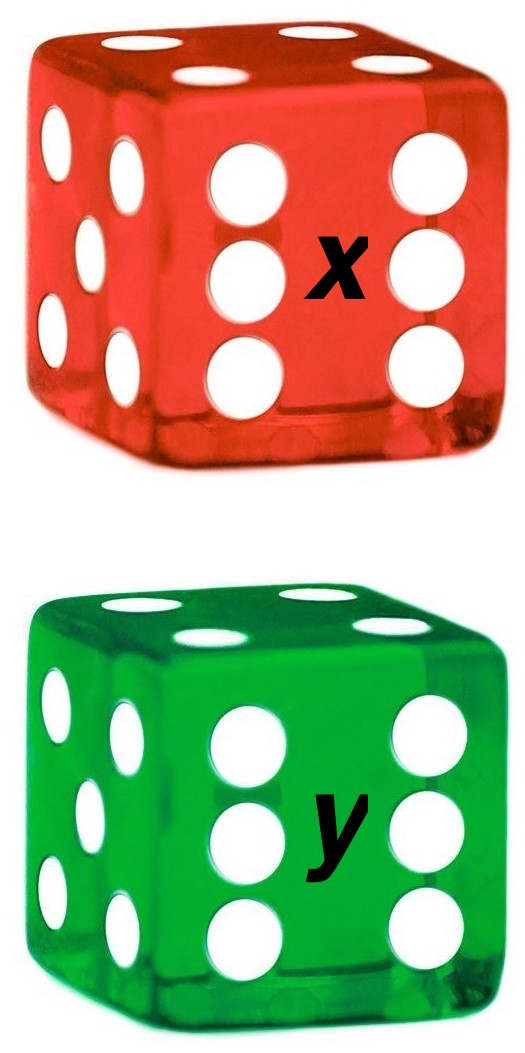
\includegraphics[width=0.5\textwidth]{img-05/color-dice}
\end{minipage}
Ara suma tots els resultats obtinguts i compara'l amb el teu company. Guanya la suma més gran. Quin deu ésser el valor més gran possible d'aquesta suma? Demana si algú de la classe ha obtingut aquest valor.
\answers{L'expressió simplificada de la suma és $4(x+y)-x^2-y^2$ i presenta un màxim a $x=y=2$. El valor màxim d'aquesta suma és 8.}
 
\end{mylist}

\section{Monomis}

\begin{theorybox}

\video[ytid=COY431F1xds]{169}{Monomis. Definició i operacions}  

Un \textbf{monomi} està format per un únic terme:   $-5\ xy^2$                 

\textbf{Coeficient}: $-5$,   \textbf{Part literal}: $xy^2$,

\textbf{Grau }(és la suma d'exponents): 3

\vspace{0.75cm}

\end{theorybox}

\vspace{2cm}
\begin{mylist}


\exer \spen En cadascun dels següents monomis escriu el seu coeficient, la seva part literal i el seu grau:

\begin{center}
\renewcommand*{\arraystretch}{1.4}
\begin{longtable}{|p{1.2in}|p{1.1in}|p{1.0in}|p{1.0in}|} \hline 
\rowcolor{lightgray} Monomi & Coeficient & Part literal & Grau \\ \hline 
$-12x^{3} $ &  &  &  \\ \hline 
$a^{4} b^{3} c$ &  &  &  \\ \hline 
$4xy^{2} $ &  &  &  \\ \hline 
\end{longtable}
\end{center}

\answers{ \begin{tabular}{|c|c|c|c|} \hline 
			\rowcolor{lightgray} Monomi & Coef & P.literal & Grau \\ \hline 
			$-12x^{3} $ & -12 & $x^3$ & 3 \\ \hline 
			$a^{4} b^{3} c$ & 1 & $a^{4} b^{3} c$ &  8  \\ \hline 
			$4xy^{2} $ & 4 & $xy^2$ & 3 \\ \hline 
		\end{tabular}
}

 \end{mylist}    

 

\subsection{Operacions amb monomis}

\begin{theorybox}


 \textbf{- Suma o resta de monomis:}           Només poden sumar o restar monomis amb la mateixa part literal. Sumam o restam els coeficients i copiam la part literal.

\begin{center}
	$\ 2x^2+5x^2-x^2=6x^2$    \quad\quad en canvi,\quad\quad    $2x^2+5x-y$  no es pot efectuar.
\end{center}
\vspace{0.25cm}

\textbf{- Producte de monomis: ``}\textit{Multiplicam coeficient amb coeficient i lletres amb lletres.''} 
\[2x^2\textrm{·}5x^3=2\textrm{·}5\ x^2\textrm{·}x^3=\ 10\ x^5\] 


\textbf{- Quocient de monomis: ``}\textit{Dividim coeficient amb coeficient i lletres amb lletres.''} 
\[4x^8:5x^5=\frac{4\ x^8}{5\ x^5}=\frac{4}{5}x^3\] 
\end{theorybox}

\begin{mylist}

\exer \spen Suma i resta els monomis equivalents.
\begin{tasks}(2)
\task $3x+5x =$ \examplebox{$8x$}
\task $11y+21y-7y =$ \examplebox{$25y$}
\task $5ab-18ab+7ab=$ \examplebox{$-6ab$}
\task $3x^5+7x^5=$
\task $4z^2+\frac{1}{2}z^2=$
\task $-x^2+\frac{1}{4}x^2=$
\task $x^4y^3+ \frac{1}{2}x^4y^3+\frac{1}{3}x^4y^3=$
\task $a-4a-(-8a+3a)+3a=$
\end{tasks}

\answers[cols=2]{[$8x$, $25y$, $-6ab$, $10x^5$, $\frac{9}{2}z^2$, $-\frac{3}{4}x^2$, $\frac{11}{6}x^4y^3$, $5a$]}

\exer \spen Fes el producte de monomis.
\begin{tasks}(2)
	\task $2x\cdot x \cdot x^2=$ \examplebox{$2x^4$}
	\task $4x^5\cdot 2x^7 =$ \examplebox{$8x^{12}$}
	\task $ \frac{1}{3}y^4 \cdot \frac{2}{5}y^2 =$
	\task $(-8x^2)\cdot \frac{1}{8}=$
	\task $(-\frac{3}{2}x^7)\cdot(-\frac{1}{3}x^4)\cdot (-x)=$
	\task $3x \cdot xy=$
	\task $5xy \cdot 3y^3 \cdot x^2y^2=$
	\task $a^2b^2 \cdot ab=$
\end{tasks}

\answers[cols=2]{[$2x^4$, $8x^{12}$, $\frac{2}{15}y^6$, $-x^2$, $-\frac{1}{2}x^{12}$, $6x^2 y$, $15x^3 y^6$, $a^3 b^3$]}

\newpage
\exer \spen Fes el quocient de monomis
 \begin{tasks}(2)
	\task $x^2:x=$\examplebox{$x$}
\task $x^3:2x^2=$\examplebox{$\frac{x}{2}$}
\task $3x^5:x^2=$
\task $\frac{8x^7}{2x^5}=$
\task $x^3:(2x^3)=$
\task $(-3)x^8:(-2x^3)=$
\task $\frac{-12x^3}{4x}=$
\task $3x^7:(-x^4)=$
\task $-9a:(3a)=$
\task $-10x^3y^2:(x^2y)=$
\task $21x^5:(-7x^4)=$
\task $-5a^4b^3:(2a^3b)=$
\end{tasks}

\answers[cols=2]{[$x$, $\frac{x}{2}$, $3x^3$, $4x^2$, $\frac{1}{2}$, $\frac{3}{2}x^5$, $-3x^2$, $-3x^3$, $-3$, $-10xy$, $-3x$, $-\frac{5}{2}a b^2$]}

\exer \spen Fes les operacions combinades. 
 \begin{tasks}(2)
	\task $(4x^2:2x)\cdot x=$\examplebox{$2x^2$}
	
\task $(-2x\cdot 5x^2):(2x)=$\examplebox{$-5x^2$}

\task $xy\cdot (x+3x)=$

\task $(12 x^3y^3 -7x^3y^3): (3x^2y)=$

\task $2\frac{x^5}{x^3}+ 2 \frac{x^4}{x^2} + 2 \frac{x^2}{x^0}=$

\task $(ab^2)\cdot a + (a^2 b)\cdot (3b)=$

\task $(ab):a - (7b^2+b^2):b=$

\task $\frac{\frac{x^2y^2}{xy}+\frac{3}{2}xy+\frac{7x^4y}{3x^3}}{\frac{3}{2}y}=$
 \end{tasks}

\answers[cols=2]{[$2x^2$, $-5x^2$, $4x^2 y$, $\frac{5}{3} x y^2$, $6x ^2$, $4 a^2 b^2$, $-7b$, $\frac{29}{9}x$]}

\end{mylist}


\section{Operacions amb polinomis}

\begin{theorybox}
\begin{multicols}{2}
	\centering
 \videonw[ytid=dOSn5n9k09]{170}{Polinomis: Definició. Suma i resta.}
 \videonw[ytid=3M7-s6U2oXw]{171}{Producte de polinomis}                     
 \end{multicols}

 Un \textbf{polinomi} està format per la suma o resta de \textbf{molts} de \textbf{monomis}. 
 
 Per exemple $9x^2-2x+5$, està format per 3 termes. Té grau 2 que és el major grau dels seus monomis. El seu terme independent és 5 (correspon al terme de grau 0) .
\end{theorybox}

\newpage
\begin{mylist}
	
	
\exer \spen Completa la taula

\begin{center}
	\renewcommand*{\arraystretch}{1.6}
	\begin{longtable}{|p{1.2in}|p{1.1in}|p{1.0in}|p{1.0in}|} \hline 
		\rowcolor{lightgray} Polinomi & N. Termes & Grau & Terme \par independent \\ \hline 
		$5x^{4} +7x^{2}$ &  &  &  \\ \hline 
		$6x^{2} +10-2x^{3} $ &  &  &  \\ \hline 
		$3x^{4}-5x^{3}+x^2+1 $ &  &  &  \\ \hline 
		$2xy^{3} -x^{5} +7x^{2} y^{2}$ &  &  &  \\ \hline 
	\end{longtable}
\end{center}
 
 \answers{\par 	\begin{tabular}{|c|c|c|c|} \hline 
 			\rowcolor{lightgray} Poli. & Termes & Grau & T.I. \\ \hline 
 			$5x^{4} +7x^{2}$ & 2 & 4 & 0 \\ \hline 
 			$6x^{2} +10-2x^{3} $ & 3  & 3 &  10 \\ \hline 
 			$3x^{4}-5x^{3}+x^2+1 $ & 4 & 4 & 1 \\ \hline 
 			$2xy^{3} -x^{5} +7x^{2} y^{2}$ & 4 & 5 & 0 \\ \hline 
 		\end{tabular}}

\exer \spen Sigui el polinomi $P(x)=x^{3} -3x+2$. Troba els següents valors numèrics de $P(x)$:


 $P(0)=$
  
  $P(1)=$
  
   $P(-1)=$
   
   $P(-2)=$ 
   
   
    $P(1/2)=$   


\answers{[$2$, $0$, $4$, $0$, $\frac{5}{8}$]}


\exer \spen  Realitza les següents sumes de polinomis:

\begin{tasks}(1)
	\task  $(-x^{3} +x-5)+(2x^{2} +5x+4)+(-4x^{3} -2x^{2} +3x)=$
	
	\task   $(x^{2} +4)+(-2x+4)+(-6x^{3} +3x^{2} +x+1)-x^{2}= $
\end{tasks}

\answers{[$-5x^3+9x-1$, $-6x^3+3x^2-x+9$]}


\exer  \spen Realitza les següents diferències. (Canvia tots els signes del subtrahend) 
\begin{tasks}(1)
\task   $(5x^{2} +2)-(-2x)=$

\task   $(-2x^{3} +4x)-(-2x-1)=$            

\task  $ (7x^{2} -2x)-(3x^{3} +4x^{2} -x+1)=$
\end{tasks}

\answers{[$5x^2+2x+2$, $-2x^3+6x+1$, $-3x^3+3x^2-x-1$]}

\begin{comment}

\exer  Escriu el polinomi oposat (canviat de signe) de cadascun dels següents polinomis: 
\begin{tasks}(3)
    \task $2x^{3} -2x^{2} -3x+9$   
	\task  $-5x$   
	\task  $-x^{3} +7x$ 
\end{tasks}


\exer  Obté el valor del polinomi $P(x)= 4x^{3} -x^{2} +1$ en $x=2$. Quin valor pren el polinomi oposat de  $P$ en $x=2$? 

\end{comment}

\exer  Considera els polinomis $P(x)= x^{2} -x+1$, $Q(x)= -x^{3} +2x-3$, així com el polinomi suma $S=P+Q$. Troba els valors de cadascun d'ells per a $x=-2$, és a dir, calcula $P(-2)$, $Q(-2)$ i $S(-2)$. Investiga si existeix alguna relació entre aquests tres valors.   

\answers{El polinomi suma $S(x)=-x^3+x^2+x-2$; els valors numèrics $P(-2)=7$, $Q(-2)=1$ i $S(-2)=8$. Es compleix que $S(-2)=P(-2)+Q(-2)$. }

\exer  Fes aquestes multiplicacions de monomi per polinomi:
\begin{tasks}(2)
	\task $x\cdot (x^2+3x-1)=$
	\task $3x\cdot (-2x+5)=$
	\task $-2x^2\cdot (3x^5 - 4x^2 + 8x)=$
	\task $\frac{3}{2}x^3\cdot (6x^4 + 2)=$
\end{tasks}  

\answers{[$x^3+3x^2-x$, $-6x^2+15x$, $-6x^7+8x^4-16x^3$, $9x^7+3x^3$]}

\exer \spen De cadascun dels següents polinomis extreu els factors que siguin comuns als seus monomis:

\begin{tasks}(2)
	\task  $2x^2+2x+2=$ \examplebox{$2\cdot (x^2+x+1)$}
	\task  $x^2+x=$ \examplebox{$x\cdot (x+1)$} 
	\task  $15x^2+5x=$
	\task  $-16x^2-4x-8=$   
	\task  $-10x^{3} -15x^{2} +20x=$   	
	\task  $30x^{4} +24x^{2}=$
\end{tasks}

\answers{[$2(x^2+x+1)$, $x(x+1)$, $5x(3x+1)$, $-4(4x^2+x+2)$, $-5x(2x^2+3x-4)$, $6x^2(5x^2+6)$]}

\exer  Efectua els següents productes de polinomis:
\begin{tasks}(2)
	\task $(-2x)\cdot (3x^{2} -4)=$
	\task $(2x^{3} +1)\cdot (-4x+5)=$
	\task $(4x^{3} -x^{2} -1)\cdot (2x+6)=$
	\task $(-1)\cdot (8x^{2} +7x-9)=$
\end{tasks}  

 \answers{[$-6x^3+8x$, $-8x^4+10x^3-4x+5$, $8x^4+22x^3-6x^2-2x-6$, $-8x^2-7x+9$]}

\exer  Calcula i simplifica els següents productes: 

\begin{tasks}(2)
	\task   $x\cdot (-2x+4)$     
	\task   $(2x-3)\cdot (3x+2)$    
	\task   $(a-2)\cdot (4-3a)$  
	\task   $(3a-b^{2} )\cdot (2b-a^{2} )$ 
\end{tasks}

\answers{[$-2x^2+4x$, $6x^2-5x-6$, $-3a^2+10a-8$, $-3a^3 + a^2b^2+6ab-2b^3$]}


\exer[1]  Realitza els següents productes de polinomis:

\begin{tasks}(2)
	\task  $x\cdot (-3x^{2} +4x+2)\cdot x^{2} $  
	\task $(-2x+1)\cdot (5x^{2} -x+3)\cdot (-x)$  
	\task  $(3a-1)\cdot (2-a)\cdot (5-4a)$
\end{tasks}
\answers[cols=1]{[$-3x^5+4x^4+2x^3$, $10x^4-7x^3+7x^2-3x$, $12\,a^3-43\,a^2+43\,a-10$]}

\end{mylist}

\subsection{Divisió de polinomis}

\begin{theorybox}
	\begin{multicols}{2}
		\centering
	 \videonw[ytid=YBETI9pfbRc]{46}{Divisió de polinomis. Regla general}
	 \videonw[ytid=_R9YJW_bwus]{47}{Divisió de polinomis. Regla de Ruffini}                     
	 \end{multicols}
En una divisió de dos polinomis
\[ 
	\begin{array}{lll}
	D(x) & & |\underline{d(x)\quad} \\
	\underbrace{R(x)} & & Q(x)
	\end{array}
\]

$D(x)$ s'anomena dividend, $d(x)$ divisor, $Q(x)$ quocient i $R(x)$ el residu. En el cas que el residu sigui zero, es diu que la \textbf{divisió és exacta}.

La comprovació que una divisió està ben feta és:
\[ \boxed{ D(x)= Q(x)\cdot d(x) + R(x)}  \]

Si el divisor és de la forma $x-a$ o $x+a$, aleshores podem utilitzar la \textbf{regla de Ruffini}. Recorda que quan falta algun terme en el dividend cal afegir zeros quan feim Ruffini.
   

   
\end{theorybox}

\pagebreak

\begin{example}
 	$\bullet$ Comprova que els càlculs que tens a continuació reflecteixen la divisió del polinomi
	
	 $p(x)=6x^{4} +5x^{3} +x^{2} +3x-2$ entre el polinomi $q(x)=2x^{2} -x+3$:
	
	
	\[ \begin{array}{l} {\, \, \, \, 6x^{4} +5x^{3} +x^{2} +3x-2\quad \quad \quad \quad \underline{|}\underline{\quad 2x^{2} -x+3}\underline{\quad }} \\ {\underline{-6x^{4} +3x^{3} -9x^{2} }\, \, \, \, \, \, \, \, \, \, \, \, \, \, \, \, \, \, \, \, \, \, \, \, \, \, \, \, \, \, \, \, \, \, \, \, \, \, \, \, \quad 3x^{2} +4x-2\, } \\ {\, \, \, \, \, \, \, \, \, \, \, \, \, \, \, \, 8x^{3} -8x^{2} +3x-2} \\ {\, \, \, \, \, \, \, \, \, \, \, \, \underline{-8x^{3} +4x^{2} -12x}} \\ {\, \, \, \, \, \, \, \, \, \, \, \, \, \, \, \, \, \, \, \, \, \, \, \, -4x^{2} -9x-2} \\ {\, \, \, \, \, \, \, \, \, \, \, \, \, \, \, \, \, \, \, \, \, \, \, \, \, \, \, \, \underline{4x^{2} -2x+6}} \\ {\, \, \, \, \, \, \, \, \, \, \, \, \, \, \, \, \, \, \, \, \, \, \, \, \, \, \, \, \, \, \, \, \, \, \, \underbrace{-11x+4} } \end{array} \]
	
	
	$\bullet$ Realitza aquesta divisió $(x^3+5x-2) : (x-4)$ per la regla de Ruffini:
	
	\[ \begin{array}{r|rrrr}  & 1 & 0 & 5 & -2\\ 4 &  & 4 & 16 & 84 \\ \hline  & 1 & 4 & 21 & \examplebox{ 82 }\end{array} \]
	
	El quocient és $Q(x)=x^2+4x+21$ i el residu de la divisió $R=82$.
	\end{example}

\begin{mylist}

\exer[1]  Divideix els següents polinomis:   
\begin{tasks} 
   \task \makebox[6cm]{$3x^{3} +4x^{2} -9x+7$} entre \quad $x^{2} +2x-1$
   \task \makebox[6cm]{$-6x^{3} +2x^{2} +3x+4$} entre \quad $3x^{3} +x^{2} -2x+1$
   \task \makebox[6cm]{$-6x^{4} -13x^{3} -4x^{2} -13x+7$} entre\quad $-3x^{2} -2x+1$ 
   \task \makebox[6cm]{$3x^{5} -9x^{4} +7x^{3} +4x^{2} -14x+14$} entre \quad $x^{3} -2x^{2} -x+3$ 
   \task \makebox[6cm]{$x^{5} -4x-6$} entre \quad $x^{2} +3$ 
\end{tasks}
\answers[cols=1]{[$Q=3x-2$; $R=-2x+5$, $Q=-2$; $R=4x^2-x+6$, $Q=2x^2+3x$; $R=-16x+7$, $Q=3x^2-3x+4$; $R=-x+2$, $Q=x^3-3x$; $R=5x-6$]}

\exer[1]  Efectua les següents operacions utilitzant \textbf{la regla de Ruffini} i indica quines d'elles són exactes.
\begin{tasks} 
  \task  $\left(3x^2-\ 2x\ +\ 5\right):\left(x+3\right)$
  \task  $\left(x^4-\ 16\right):\left(x-2\right)$
  \task  $\left(x^4-x^3+x^2-x+1\right):\left(x-1\right)$
   \task $\left(7x^5-\ 4x^3+7x-\ 5\right):\left(x+2\right)$
\end{tasks}
\answers[cols=1]{[$Q=3x-11$; $R=38$, $Q=x^3+2x^2+4x+8$; $R=0$, $Q=x^3+x$; $R=1$, $Q=7x^4-14x^3+24x^2-48x+103$; $R=-211$]}


 


\exer  Efectua les divisions de polinomis pel mètode que creguis més convenient: 

\begin{tasks} 
	\task  \makebox[6cm]{$2x^{3} +x^{2} -12x+7$} entre \quad $x+3$    
	\task  \makebox[6cm]{$-4x^{4} +8x^{3} +7x^{2} -21x+8$} entre \quad $2x^{2} -3x+1$
	\task  \makebox[6cm]{$-3x^{5} -2x^{3} +9x^{2} +6x-14$} entre \quad $-x^{3} -2x+3$
\end{tasks}

\answers[cols=1]{[$Q=2x^2-5x+3$; $R=-2$, $Q=-4x^4+8x^3+7x^2-21x+8$; $R=2x^2-3x+1$, $Q=3x^2-4$; $R=-2x-2$]}

\exer  Troba dos polinomis tals que en dividir-los obtinguem $q(x)=x^{2} -2x-1$ com a polinomi quocient i $r(x)=2x^{2} -3$ com a residu. 

\answers{Hi ha infinites solucions. Per exemple, si ens inventam el divisor=$2x+3$, el dividend=quocient·divisor + residu = $(x^2-2x-1)(2x+3)+2x^2-3=2x^3+x^2-8x-6$} 

\end{mylist}


\section{Identitats notables}


\begin{theorybox}
	
	\video[ytid=xfVp1cXpKb4]{172}{Identitats notables}
	
	\makebox[4cm][l]{Quadrat d'una suma:}   ${\left(\boldsymbol{a}\boldsymbol{+}\boldsymbol{b}\right)}^{\boldsymbol{2}}\boldsymbol{=\ }{\boldsymbol{a}}^{\boldsymbol{2}}\boldsymbol{+}\boldsymbol{2}\boldsymbol{\textrm{·}}\boldsymbol{a}\boldsymbol{\textrm{·}}\boldsymbol{b}\boldsymbol{+}{\boldsymbol{b}}^{\boldsymbol{2}}$ 
	
	\makebox[4cm][l]{Quadrat d'una diferència:}   ${\left(\boldsymbol{a}\boldsymbol{-}\boldsymbol{b}\right)}^{\boldsymbol{2}}\boldsymbol{=\ }{\boldsymbol{a}}^{\boldsymbol{2}}\boldsymbol{-}\boldsymbol{2}\boldsymbol{\textrm{·}}\boldsymbol{a}\boldsymbol{\textrm{·}}\boldsymbol{b}\boldsymbol{+}{\boldsymbol{b}}^{\boldsymbol{2}}$       
	
	\makebox[4cm][l]{Suma per diferència:} $\left(\boldsymbol{a}\boldsymbol{+}\boldsymbol{b}\right)\boldsymbol{\textrm{·}}\left(\boldsymbol{a}\boldsymbol{-}\boldsymbol{b}\right)\boldsymbol{=\ }{\boldsymbol{a}}^{\boldsymbol{2}}\boldsymbol{-}{\boldsymbol{b}}^{\boldsymbol{2}}$
	\vspace{0.5cm}
\end{theorybox}

\begin{mylist}

\exer \spen  Desenvolupa les identitats:

\begin{tasks}(2)
	\task  $(1+x)^{2}= $    
	
	\task  $(-x+2)^{2}= $     
	
	\task  $(x-2)^{2} =$ 
	
	\task  $(2a-3)^{2}= $      
	
	\task $\left(x^{2} +1\right)^{3}= $      
	
	\task $(2b-4)^{3}= $
\end{tasks}

\answers[cols=2]{[$1+2x+x^2$, $x^2-4x+4$, $x^2-4x+4$, $4a^2-12a+9$, Atenció 3: $x^6+3x^4+3x^2+1$, Atenció 3: $8b^3-48b^2+96b-64$]}


\exer \spen  Efectua aquests productes:

\begin{tasks}(2)
	\task  $(3x+2)\cdot (3x-2)=$    

	\task  $(2x+4y)\cdot (2x-4y)=$   

	\task  $(4x^{2} +3)\cdot (4x^{2} -3)=$

	\task  $(3a-5b)\cdot (3a+5b)=$   
	
	\task  $(x^{3} -4)\cdot (x^{3} +4)=$ 

	\task  $\left(-x^{2} +5x\right)\cdot \left(x^{2} +5x \right)=$ 
\end{tasks}

\answers{[$9x^2-4$, $4x^2-16y^2$, $16x^4-9$, $9a^2-25b^2$, $x^6-16$, $-x^4+25x^2$]}

\exer \spen  Desenvolupa les següents potències: 

\begin{tasks}(2)
	\task  $(3x-y)^2=$
	
	\task  ${\left(2a\ +\ \frac{x}{2}\right)}^2=$   
	
	\task  ${\left(4y-\ \frac{2}{y}\right)}^2=$ 
	
	\task  $\left(5a+a^2\right)^2=$
	 
	\task  $\left( -a^2+2b^2 \right)^2=$ 
	 
	\task  ${\left(\frac{2}{3}y-\ \frac{1}{y}\right)}^2=$ 
\end{tasks}

\answers{[$9x^2-6xy+y^2$, $4a^2+2ax+\frac{x^2}{4}$, $16y^2-16+\frac{4}{y^2}$, $25a^2+10a^3+a^4$, $a^4-4a^2b^2+4b^4$, $\frac{4y^2}{9}-\frac{4}{3}+\frac{1}{y^2}$]}

\pagebreak
\exer \spen Expressa com quadrat d'una suma o d'una diferència les següents expressions algebraiques:

\begin{tasks}(2)
	\task  ${a}^{2} - 6{a +} 9 = \left(\square - \square \right)^2$   
	\task  $4{x}^{2} + 4x + 1 =$   
	\task  ${b}^{2} - 10{b} + 25=$
	\task  $4{y}^{2} - 12{y} + 9 =$   
	\task  ${a}^{4} + 2{a}^{2} +1=$    
	\task  ${y}^{4} + 6x{y}^{2} + 9{x}^{2}=$
\end{tasks}

\answers{[$(a-3)^2$, $(2x+1)^2$, $(b-5)^2$, $(2y-3)^2$, $(a^2+1)^2$, $(y^2+3x)^2$]}

\vspace{0.5cm}

\exer \spen  Expressa com suma per diferència les següents expressions

\begin{tasks}(2)
	\task  $9x^2-25 = \left(\square + \triangle \right) \cdot \left(\square - \triangle \right)  $    
	\task  $4 a^4 - 81 b^2 =$   
	\task  $49-25x^2 =$ 
	\task  $100 a^2 -64=$
\end{tasks}

 \answers{[$(3x+5)(3x-5)$, $(2a^2+9b)(2a^2-9b)$, $(7+5x)(7-5x)$, $(10a+8)(10a-8)$]} 
\vspace{0.5cm}

\exer  Realitza les següents divisions de polinomis a partir de la conversió del dividend en la potència d'un binomi o en un producte de la forma suma per diferència:

\begin{tasks}(2)
	\task $x^{2} +12x+36$    entre $x+6$      
	\task  $4x^{4} -16x^{2} $ entre $2x^{2} -4x$ 
	\task  $9x^{2} -24x+16$ entre $3x-4$     
	\task  $x^{2} -4$  entre $x+2$   
\end{tasks}

\answers[cols=1]{[$(x+6)^2 / (x+6)=x+6$, $(2x^2+4x)(2x^2-4x)/(2x^2-4x)=2x^2+4x$, $(3x-4)^2/(3x-4)=3x-4$, $(x+2)(x-2)/(x+2)=x-2$]}
\vspace{0.5cm}


\exer \hot  Obté les fórmules dels quadrats dels següents trinomis:

\begin{tasks}(2)
	\task $(a+b+c)^{2} $    
	\task  $(a-b+c)^{2} $ 
\end{tasks}

\answers{[$a^2+b^2+c^2+2ab+2ac+2bc$, $a^2+b^2+c^2-2ab+2ac-2bc$]}


\end{mylist}


\section{Introducció a les fraccions algebraiques}

\begin{theorybox}

 Una fracció algebraica és el quocient de dos polinomis $\frac{D\left(x\right)}{d\left(x\right)}$

 Si la divisió $D(x):d(x)$ és exacta, la fracció serà en realitat un polinomi.

 Per \textbf{sumar/restar fraccions} necessitam denominador comú:
\[\frac{2x}{x-1}+\frac{3}{x+2}=\frac{2x\textrm{·}(x+2)}{(x-1)(x+2)}+\frac{3(x-1)}{(x-1)(x+2)}=\frac{2x\textrm{·}\left(x+2\right)+3\left(x-1\right)}{(x-1)(x+2)}=\frac{2x^2+7x-3}{x^2+x-2}\] 
Per \textbf{multiplicar fraccions}, multiplicam ``en línia´´:
\[\frac{2x}{x-1}\textrm{·}\frac{3(x+2)}{x+1}=\frac{2x\textrm{·}3(x+2)}{(x-1)(x+1)}=\frac{6x^2+12x}{x^2-1}\] 
Per \textbf{dividir fraccions}, multiplicam ``en creu´´:
\[\frac{2x}{x-1}:\frac{3(x+2)}{x+1}=\frac{2x\textrm{·}(x+1)}{3(x-1)(x+2)}=\frac{2x^2+2x}{3x^2+3x-6}\] 
\end{theorybox}

\begin{mylist}

\exer[1]  Efectua els següents càlculs: 

\begin{tasks}(2)
	\task  $\frac{1}{x+2} +\frac{2}{x-1} $   
	\task $\frac{x-2}{x^{2} -x} -\frac{5}{x} $   
	\task $\frac{-x+1}{x+3} \cdot \frac{3x^{2} }{x+1} $   
	\task $\frac{2+x}{x^{2} } :\frac{x}{x-3} $
\end{tasks}
\answers{[$\frac{3x+3}{x^2+x-2}$, $\frac{-4x+3}{x^2-x}$, $\frac{-3x^3+3x^2}{x^2+4x+3}$, $\frac{x^2-x-6}{x^3}$]}

\exer[1]  Realitza les següents operacions alterant, en cada apartat, solament un dels denominadors, i el seu respectiu numerador: 

\begin{tasks}(2)
	\task $\frac{-2x^{2} -x+1}{x^{3} } +\frac{3x+1}{x^{2} } $    
	\task $\frac{2x-1}{x^{2} -2x} -\frac{3}{x-2} $
\end{tasks}
\answers{[$\frac{x^2+1}{x^3}$, $\frac{-x-1}{x^2-2x}$]}

\exer  Calcula els següents quocients (treu factor comú del numerador):  

\begin{tasks}(2)
	\task  (2\textit{x}${}^{3}$ $-$ 8\textit{x}${}^{2}$ + 6\textit{x}) : 2\textit{x    }
	\task  (5\textit{a}${}^{ 3}$ + 60\textit{a${}^{ 2}$} $-$ 20) : 5  
	\task  (16\textit{x}${}^{3}$ + 40\textit{x}${}^{2}$) : 8${x}^{2 }$   
	\task  (6\textit{x}${}^{2}$y${}^{3}$ $-$ 4\textit{xy${}^{2}$}) : \textit{xy}${}^{2}$
\end{tasks}
\answers{[$x^2-4x+3$, $a^3+12a^2-4$, $2x+5$, $6xy-4$]}


\end{mylist}
 
\begin{resolt}{Simplifica la fracció algebraica \[ \frac{x^2-2x}{x^2 - 4} \]}
	La primera passa consisteix en factoritzar el numerador i el denominador. Per això ens fixam si podem treure factor comú i/o identificam alguna identitat notable.
	
	\[ \frac{x^2-2x}{x^2 - 4} = \frac{x \cdot \cancel{(x-2)}}{(x + 2)\cdot \cancel{(x-2)}} = \frac{x}{x + 2} \]
	
	Finalment, hem eliminat els factors que estan repetits al numerador i denominador.
\end{resolt}
 
\begin{mylist}

\exer  Comprova les següents identitats simplificant l'expressió del costat esquerre de cada igualtat: 

\begin{tasks}(2)
	\task $\frac{6a^{8} b^{2} }{2a^{3} b} =3a^{5} b$    
	\task  $\frac{8x^{3} y-2xy^{2} }{4xy} =2x^{2} -\frac{1}{2} y$ 
	\task $\frac{4x^{2} +2x}{2x-8} =\frac{2x^{2} +x}{x-4} \quad $   
	\task  $\frac{6a^{2} b^{2} -4a^{2} b^{3} +4ab}{2ab^{2} -8a^{2} b} =\frac{3ab-2ab^{2} +2}{b-4a} $
\end{tasks}

\exer  Simplifica les següents fraccions traient factor comú:

\begin{tasks}(2)
	\task  $\frac{3x^{2} +6x}{9x^{2} +18} $   
	\task  $\frac{a^{3} -7a^{2} }{3a^{3} +5a^{2} } $   
	\task  $\frac{x^{2} y^{2} -7xy^{2} }{2xy} $   
	\task $\frac{a^{2} b^{2} -ab}{a^{3} b+ab} $
\end{tasks}


\answers[cols=1]{[$\frac{3x(x+2)}{3(3x^2+6)}=\frac{x(x+2)}{3x^2+6}$,
	$\frac{a^2(a-7)}{a^2(3a+5)}=\frac{a-7}{3a+5}$,
	$\frac{ay(xy-7y)}{2xy}=\frac{y(x-7)}{2}$,
	$\frac{ab(ab-1)}{ab(a^2+1)}=\frac{ab-1}{a^2-1}$]}


\exer[1] En cadascuna de les següents fraccions algebraiques escriu, quan sigui possible, el polinomi numerador, o denominador, en forma de potència d'un binomi o de suma per diferència per, posteriorment, poder simplificar cada expressió: 

\begin{tasks}(4)
	\task  $\frac{x^{2} -4}{3x+6} $    
	\task $\frac{2x^{2} -16x+32}{x^{2} -16} $   
	\task  $\frac{6-4a}{4a^{2} -9} $
	\task  $\frac{x^2+2x}{x^2-4}$
\end{tasks}
\answers[cols=2]{[$\frac{x-2}{3}$, $\frac{2(x-4)}{x+4}$, $\frac{-2}{2a+3}$, $\frac{x}{x-2}$]}
\end{mylist}




\pagebreak
\begin{activitats}
	
\begin{mylist}

\exer  Una empresa majorista de viatges està confeccionant una oferta per distribuir-la en diferents agències de viatges. Es tracta d'un viatge amb avió, d'anada i tornada, a Madrid el preu de la qual dependrà del nombre final de viatgers. Les dades concretes són: 

\begin{tasks}
	\task[-]  Si no hi ha més de 100 persones interessades, el vol costarà 150 euros per persona.
	\task[-]  Si hi ha més de 100 persones interessades, per cada viatger que passi del centenar el preu del viatge es reduirà en 1 euro. No obstant això, el preu del vol en cap cas serà inferior a 90 euros.
\end{tasks}
Estudia i determina el preu final del vol, per persona, en funció del nombre total de viatgers. Així mateix, expressa la quantitat que ingressarà l'empresa segons el nombre de viatgers. 

\answers{	Anomenarem $n$ al nombre de viatgers, $p$ al preu per viatger i $T$ a la quantitat total ingressada per l'empresa.\par
	Tots els valors de les variables són nombres enters.\par
	Si $n <101$: $P = 150$; $T = 150N$\par
	Si $n = 100 + x (0 <x <61)$: $p = 150 - x$; $T = 15 000 + 50x - x^2$\par
	Si $n> 160$: $p = 90$; $T = 90N.$}

\exer  En aquest exercici es mostra un \textit{truc} mitjançant el qual anem a endevinar el nombre que resulta després de manipular repetidament un nombre desconegut. Converteix en una expressió algebraica les successives alteracions del nombre desconegut i justifica el que ocorre.  
  
  \begin{itemize}
 \item Digues-li a un company que escrigui en un paper un nombre parell i que no ho mostri   

 \item Que ho multipliqui per 5

\item Que al resultat anterior li sumi 5 

\item  Que multipliqui per 2 el resultat

 \item Que al resultat anterior li sumi 10

 \item Que multipliqui per 5 

 \item  Que divideixi entre 100 la darrera quantitat 
 
 \item  Que al resultat precedent li resti la meitat del nombre que va escriure

\end{itemize} 

Independentment del nombre desconegut original quin nombre ha sorgit?

\answers{	Si anomenam $2n$ al nombre parell inicial, la seqüència d'operacions dóna lloc a $\frac{[(10n+5)\cdot 2 -10]\cdot 5}{100}-n = 0$. 
}

\exer  Els responsables d'una empresa, en previsió d'uns futurs alts i baixos en les vendes dels productes que fabriquen, pensen proposar als seus treballadors a la fi de l'any 2014 el següent: 
\begin{itemize}
\item  La disminució dels sous, per al proper any 2015, en un 10\%. 

\item  Per 2016 ofereixen augmentar un 10\% els salaris de 2015.

\item  En general, suggereixen que el sou disminueixi un 10\% cada any imparell i que augmenti un 10\% cada any parell. 
\end{itemize}

 Si finalment s'aplica aquest pla, estudia si els treballadors recuperaran l'any 2016 el salari que tenien en 2014. Analitza què ocorre amb els sous després del pas de molts anys.

\answers{  Si anomenem $s$ al salari de 2014, els salaris dels anys successius són:\par
	$0,9 s$; $0,99 s$; $0,891 s$; $0,9801 s$; $0,88209 s$; $0,970299 s$; ...
	Els salaris són cada vegada menors que dos anys abans.}


\begin{comment}
\exer  Els responsables de l'anterior empresa, després de rebre l'informe d'una consultora, alteren la seva intenció inicial i van a proposar als seus treballadors, a la fi de l'any 2014, el següent: 


\exer 
\exer  Un augment dels sous, per al proper any 2015, d'un 10\%. 

\exer  Per 2016, una reducció del 10\% sobre els salaris de 2015.

\exer  En general, suggereixen que el sou augmenti un 10\% cada any imparell i que disminueixi un 10\% cada any parell. 




 Si s'aplica el nou pla, analitza si el salari dels treballadors de l'any 2016 coincidirà amb el que tenien en 2014. Estudia com evolucionen els sous després del pas de molts d'anys.

\end{comment}



\exer  Observa si hi ha nombres pels quals les següents expressions no poden ser avaluades:

\begin{minipage}{0.22\textwidth}
	\begin{tasks}
		\task  $\frac{x-3}{x+1} $  
		\task $\frac{2x-1}{(x-5)\cdot (2x+7)} $   
		\task $\frac{x}{x^{2} -2x+1} $   
		\task $\frac{x+y-2}{x^{2} +3y^{2} } $
	\end{tasks}
\end{minipage}
\begin{minipage}{0.2\textwidth}
	\centering
	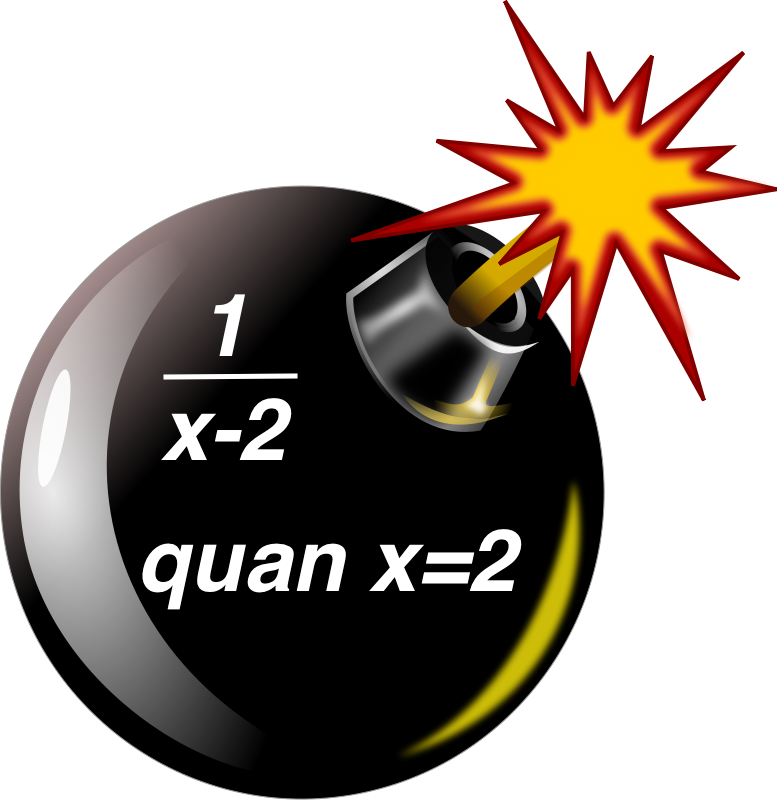
\includegraphics[width=0.85\textwidth]{img-05/bomb}
\end{minipage}

\answers{[Per a $x=-1$, Per a $x=5$ ni $x=-7/2$, Per a $x=1$, Es pot avaluar per tot $x$; $y$]}

\begin{comment}
\exer  Una persona té estalviats 3000~€ i decideix dipositar-los en un producte bancari amb un tipus d'interès anual del 2,5~\%. Si decideix recuperar els seus estalvis al cap de dos anys, quin serà la quantitat total de la qual disposarà?
\end{comment}

\exer  Construeix un polinomi de grau 2, $P(x)$, tal que $P(-2)=6$.

\answers{Per exemple: $(x+2)^2 + 6 = x^2 + 4x + 10$}

\exer  Considera els polinomis $p(x)=2x^{3} -x^{2} +4x-1$, $q(x)=-x^{4} -3x^{3} +2x^{2} -x-5$ i $r(x)=x^{2} -3x+2$ . Fes les següents operacions:  

\begin{tasks}(2)
	\task  $p+q+r$   
	\task $p-q$   
	\task $p\cdot r$   
	\task $p\cdot r-q$
\end{tasks}

\answers[cols=1]{ $p+q+r=-x^4-x^3+2\,x^2-4$, \par
	 $p-q=x^4+5\,x^3-3\,x^2+5\,x+4$,    \par
	 $p\cdot r=2\,x^5-7\,x^4+11\,x^3-15\,x^2+11\,x-2$,    \par
	 $p\cdot r-q=2\,x^5-6\,x^4+14\,x^3-17\,x^2+12\,x+3$}

\pagebreak
\exer  Calcula els productes:

\begin{tasks}
	\task  $\left(\frac{3ax}{2} -\frac{y}{5} \right)\cdot \left(\frac{-by}{3} \right)$  
	\task  $\left(0'1x+0'2y)\right)\cdot \left(0'3x-0'2y\right)$  
	\task  $\left(x-y\right)\cdot \left(y-1\right)\cdot \left(x+a\right)$
\end{tasks}

\answers{[$\frac{by^2}{15}-\frac{1}{2}abxy$, $0.03x^2 + 0.04 xy - 0.04 y^2$, $a x y - a x - a y^2 + a y + x^2 y - x^2 - x y^2 + x y$]}

\exer  Calcula els quocients: 
\begin{tasks}
	\task  $(4x^{3} ):(x^{2} )$ 
	\task  $\left(4x^{3} y^{3} z^{4} \right):\left(3x^{2} yz^{2} \right)$  
	\task  $\left(x^{4} -4x^{2} y+4y^{2} \right):\left(x^{2} -2y\right)$
\end{tasks}

\answers[cols=2]{[$4x$, $\frac{4}{3}xy^2 z^2$, $x^2-2y$]}

\exer  Realitza les operacions amb les fraccions algebraiques:  

\begin{tasks}
	\task  $\frac{x-1}{x^{2} } +\frac{2x-1}{x} $  
	\task  $\frac{2x+3}{x} +\frac{5}{x+1} $  
	\task $\frac{x-1}{x^{2} -3x} -\frac{2-x}{x} $
	\task $\frac{x-1}{x^{2} -3x} \cdot \frac{2-x}{x} $  
	\task $\frac{x-1}{x^{2} -3x} :\frac{2-x}{x} $
\end{tasks}

\answers[cols=2]{[$\frac{2x^2-1}{x^2}$, $\frac{2x^2+10x+3}{x(x+1)}$,
	 $\frac{x^2-4x+5}{x(x-3)}$, $\frac{-x^2+3x-2}{x^2 (x-3)}$, $\frac{x-1}{(x-3)(2-x)}$]}

\exer  Troba un polinomi $p(x)$ tal que en dividir $p(x)$ entre $q(x)=x^{3} -x^{2} +2x-3$ s'obtingui com a residu $r(x)=-3x^{2} +1$.  

\answers{Hi ha infinites solucions. Ens inventam un quocient, per exemple quocient=$x+1$, aleshores dividend = quocient·divisor + residu $\rightarrow$ dividend = $(x+1)(x^3-x^2+2x-3)+(-3x^2+1)=x^4-2x^2-x-2$}


\exer  Calcula les potències: 
\begin{tasks}
	\task  $(x+2y-z)^{2} $  
	\task  $(x-3y)^{3} $  
	\task  $\left(\left. a+\frac{b}{3} \right)\right. ^{2} $  
	\task  $(x^{2} -2z^{3} )^{2} $
\end{tasks}


\answers[cols=1]{[$x^2+4xy-2xz+4y^2-4yz+z^2$, $x^3-9x^2y+27xy^2-27y^3$, $a^2+\frac{2ab}{3}+\frac{b^2}{9}$, $x^4-4x^2 z^3 + 4z^6$]}

\exer  Analitza si els següents polinomis han sorgit del desenvolupament de potències de binomis o d'un producte \textit{suma per diferència}. En cas afirmatiu expressa la seva procedència.   

\begin{tasks}(2)
 	\task $x^{2} -6x+9$    
	\task  $x^{4} +8x^{2} +16$   
	\task  $x^{2} -25$   
 	\task $x^{2} +5$     
	\task $5x^{2} -1$   
	\task $x^{2} -8y^{2} $    
 	\task $x^{4} -1$     
	\task $x^{2} -y^{2} $    
%	\task $x^{2} -2y^{2} z^{2} $
\end{tasks}

\answers[cols=2]{[$(x-3)^2$, $(x^2+4)^2$, $(x+5)(x-5)$, $x^2+5$, $(\sqrt{5}x+1)(\sqrt{5}x-1)$, $(x+\sqrt{8}y)(x-\sqrt{8}y)$, $(x^2+1)(x^2-1)=(x^2+1)(x+1)(x-1)$, $(x+y)(x-y)$, $(x+\sqrt{2}yz)(x-\sqrt{2}yz)$]}


\exer  Analitza si el numerador i el denominador de les següents expressions algebraiques procedeixen del desenvolupament d'un binomi, o d'un producte suma per diferència, i simplifica-les:

\begin{tasks}
\task  $\frac{x^{2} +2x+1}{x^{2} -1} $   \task  $\frac{x^{4} -2x^{2} y^{2} +y^{4} }{x^{2} +y^{2} } $    \task  $\frac{xy^{3} -yx}{y^{4} -1} $
\end{tasks}

\answers[cols=1]{[$\frac{(x+1)^2}{(x+1)(x-1)}=\frac{x+1}{x-1}$, $\frac{(x^2-y^2)^2}{x^2+y^2}$, $\frac{xy(y^2-1)}{(y^2+1)(y^2-1)}=\frac{xy}{y^2+1}$]}


\exer   Efectua les següents operacions i simplifica tot el possible:

\begin{tasks}
	\task  $\frac{3}{x(3-x)} -\frac{1}{2(3-x)} $   
	\task  $3x^{4} -5x^{3} +\frac{x^{4} -1}{x^{3} } \cdot \frac{x^{5} }{x^{2} +1} $   
	\task  $\frac{x-2y}{a-b} +\frac{4x+5y}{3a-3b} $
\end{tasks}

\answers[cols=1]{[$\frac{x-6}{2x(x-3)}$, $4x^4-5x^3-x^2$, $\frac{7x-y}{3(a-b)}$]}

\exer  Simplifica tot el possible:

\begin{tasks}
 	\task  $\left(yx^{4} -\frac{y}{x^{2} } \right):\left(x^{2} +\frac{1}{x} \right)$   
	\task  $\frac{b^{3} +3ab^{2} +3a^{2} b+a^{3} }{b-a} :\frac{b+a}{b-a} $
	\task $\left(\frac{a+b}{a-b} -\frac{a-b}{a+b} \right):\frac{4}{a-b} $
\end{tasks}

\answers[cols=1]{[$\frac{y(x^3 -1)}{x}$, $(a+b)^2=a^2+2ab+b^2$, $\frac{ab}{a+b}$]}

\begin{comment}
\exer  Simplifica tot el possible:

\begin{tasks}
	\task  $\frac{\frac{1}{a+y} -\frac{1}{x} }{\frac{1}{a+y} +\frac{1}{x} } :\frac{\frac{1}{a} -\frac{1}{x+y} }{\frac{1}{a} +\frac{1}{x+y} } $   
	\task  $\left(1+\frac{1}{x} +\frac{2}{x^{2} } +\frac{3}{x^{3} } \right):\left(\frac{1}{x} -\frac{2}{x^{2} } -\frac{3}{x^{3} } \right)$   
	\task  $\frac{\frac{2}{x} -\frac{1}{y} }{\frac{3}{x} +\frac{2}{y} } \cdot \frac{\frac{1}{x} -\frac{3}{y} }{\frac{1}{x} -\frac{2}{y} } $
\end{tasks}
\end{comment}
 
\end{mylist}
 
\end{activitats}
 

 

 
\newpage
\begin{autoaval}{49}

\begin{mylist}

\exer[2]  Tradueix al llenguatge algebraic:  

\begin{tasks}(1)
	\task  Sumar 5 al triple d'un nombre  
	\task  El quadrat de la suma de dos nombres   
	\task  La tercera part d'un nombre parell 
\end{tasks}
\answers{[$3x+5$, $(x+y)^2$, $\frac{2n}{3}$]}


\exer[2]  Expressa mitjançant una expressió algebraica el volum d'un prisma de base quadrada de costat $x$ i d'altura 7 cm.
\answers{$V=7\,x^2$}

\exer[2] Calcula el valor numèric de l'expressió $\frac{x+7}{4-2y^{2} } +6xz^{2} -\frac{3}{z} $ en $x=1,\, \, y=2,\, \, z=-1$.  
\begin{comment}
\begin{tasks}(4)
\task  $-11$   
\task  $7$   
\task  $1$  
\task  $-5$
\end{tasks}
\end{comment}

\answers{7}


\exer[2]  Opera els següents monomis:
\begin{tasks}(3)
   \task $(3x)\cdot (5x^{2} )=$  
	\task  $(5x^{2} yz):(-3xz)=$  
	\task  $a^{2} b+3a^{5} b:a^{3} -2ab\cdot a=$
\end{tasks}
\answers{[$15x^3$, $-\frac{5}{3}xy$, $2a^2 b$]}

\exer[2]  Del polinomi $5x^{4} -8x^{2} -x+9$ indica el seu grau, terme independent i els monomis que ho integren. 
\answers{Grau 4; terme independent 9; 4 termes}

\exer[2]  Efectua les divisions de polinomis 

\begin{tasks}(2)
	\task  $(2x^{4} -x^{3} +4):(x^{2} +2x+2)$  
	\task $(3x^{4} -5x^{2} +x-2):(x-3)$
\end{tasks}
\answers[cols=1]{[$Q=2x^2-5x+6$; $R=-2x-8$, $Q=3x^3+9x^2+22x+67$; $R=199$]}


\exer[2]  Calcula utilitzant les identitats notables

\begin{tasks}(2)
	\task  $\left(\frac{2}{5} x-\frac{1}{3} y\right)^{2} =$  
	\task  $\left(x^{2} -1\right)\cdot \left(x^{2} +1\right)=$  
	\task  $\left(3x+2\right)^{2} =$ 
	\task   $\left(x^{2} +2\right)\cdot \left(x^{2} -2\right)-\left(x^{2} -1\right)^{2} =$
\end{tasks}
\answers[cols=2]{[$\frac{4}{25}x^2 - \frac{4}{15}xy + \frac{y^2}{9}$, $x^4 - 1$, $9x^2+12x+4$, $2x^2 -5$]}

\exer[2]  Extreu factor comú en cada expressió
\begin{tasks}(2)
   \task $5x^{2} -15x^{3} +25x^{4} =$  
	\task  $2x^{3} y^{5} -3x^{2} y^{4} +2x^{7} y^{2} +7x^{3} y^{3} =$
\end{tasks}
\answers[cols=1]{[$5x^2 \cdot (1-3x+5x^2)$, $x^2 y^2 \cdot (2 xy^3 - 3y^2 + 2 x^5 + 7xy)$]}

\exer[2]  Extreu factor comú i expressa com una identitat notable quan sigui possible
\begin{tasks}(3)
	\task $x^{3} +2x^{2} +x=$   
	\task  $x^{4} -x^{2} =$   
	\task  $3x^{4} -24x^{3} +48x^{2} =$
\end{tasks}
\answers[cols=2]{[$x (x+1)^2$, $x^2 (x+1)(x-1)$, $3x^2 (x^2-8x+16)$]}

\exer[2]  Opera i simplifica les fraccions algebraiques $(x+1):\frac{x^{2} -1}{2x} =$
\answers{$\frac{2x}{x-1}$}

\exer[2]  Efectua $\frac{3-x}{x^{2} } +\frac{1}{x} -\frac{x+5}{2x} $ =  \quad (\textit{Ajuda el mcm és} $2x^{2} $)
\answers{$\frac{-x^2-5x+6}{2x^2}$}

\end{mylist}

\end{autoaval}




\newpage
\setcounter{myenumi}{0}

\heading{FITXA DE REPÀS: OPERACIONS AMB POLINOMIS}

\begin{mylist}
\exer Suma els polinomis següents:
\begin{tasks}(2)
	\task  $\left(4x^{2} +2x-4\right)+\left(x^{2} +3x+6\right)=$  
	                
	\task  $\left(3x^{2} -2x+2\right)+\left(x^{2} -3x+6\right)=$  
	                                                         
	\task  $\left(-3x^{2} -5\right)+\left(2x^{2} +2x+6\right)=$   
	        
	\task $\left(3x^{3} +6x-5\right)+\left(2x^{3} -x^{2} +2x-2\right)=$             
\end{tasks}
\answers[cols=2]{[$5x^2+5x+2$, $4x^2-5x+8$, $-x^2+2x+1$, $5x^3-x^2+8x-7$]}

\exer  Donats els següents polinomis:  $A=x^{2} +3x-2$ i $B=-3x^{2} +5x-1$, calcula al teu  quadern.
\begin{tasks}(3)
	\task  $A-B$,   
	\task  $A+B$   
	\task $B-A$
\end{tasks}
\answers[cols=3]{[$4x^2-2x-1$, $-2x^2+8x-3$, $-4x^2+2x+1$]}

\exer  Efectua les operacions següents:
\begin{tasks}(2)
	\task   $3\cdot \left(3x^{3} +2x+5\right)=$        
	                                
	\task   $-3\cdot \left(2x^{2} -3x-4\right)=$
	
	\task   $3x^{2} \cdot \left(x^{3} +2x-6\right)=$
	
	\task   $-4x^{2} \cdot \left(6x^{4} -2x^{3} -6x\right)=$
\end{tasks}
\answers[cols=2]{[$9x^3+6x+15$, $-6x^2+9x+12$, $3x^5+6x^3-18x^2$, $-24x^6+8x^5+24x^3$]}

\exer  Extreu factor comú a cada un dels polinomis següents: 
\begin{tasks}(2)
	\task  $3x+3y+3z=$
	
	\task  $a^{2} +3a=$
	
	\task  $2x+4y+6z=$
	
	\task  $4x-8x^{2} +12x^{3} =$
	
	\task  $9a^{} +6a^{2} +3a^{3} =$
	
	\task  $2a^{2} -5a^{3} +a^{4} =$
\end{tasks}
\answers[cols=2]{[$3(x+y+z)$, $a(a+3)$, $2(x+2y+3z)$, $4x(1-2x+3x^2)$, $3a(3+2a+a^2)$, $a^2(2-5a+a^2)$]}

\exer  Realitza les multiplicacions d'aquests polinomis:                               
\begin{tasks}(2)
	\task  $\left(2x^{2} +3x+1\right)\cdot \left(x-1\right)=$   
	\task $\left(3x^{2} +x+2\right)\cdot \left(-7x+2\right)=$                                 
	\task  $\left(x^{2} +2x\right)\cdot \left(2x^{2} -2x-3\right)=$     
	\task $\left(-2x^{3} +x\right)\cdot \left(-x^{2} +3x+1\right)=$    	   
\end{tasks}
\answers[cols=1]{[$2x^3+x^2-2x-1$, $-21x^3-x^2-12x+4$, $2x^4+2x^3-7x^2-6x$, $2x^5-6x^4-3x^3+3x^3+x$]}

\exer  Simplifica les expressions següents:
\begin{tasks}(2)
	\task  $\left(x-1\right)\cdot \left(x+1\right)+\left(x^{2} +4\right)=$  	      
	\task  $\left(x-2\right)^{2} -\left(2x^{2} +1\right)=$	
	\task  $\left(x^{2} +2\right)^{2} -\left(x+1\right)\cdot \left(x-1\right)=$   	    
	\task  $3\cdot \left(x+1\right)^{2} -\left(2x+3\right)^{2} =$
\end{tasks}
\answers[cols=2]{[$2x^2+3$, $-x^2-4x+3$, $x^4+3x^2+5$, $-x^2-6x-6$]}

\exer  Descompon en factors.
\begin{tasks}(2)
	\task $x^{2} -6x+9=$                                                             
	\task   $x^{3} -9x=$	
	\task  $3x^{2} +6x+3=$                                                              
	\task  $x^{4} -x^{2} =$
\end{tasks}
\answers[cols=2]{[$(x-3)^2$, $x(x+3)(x-3)$, $3(x+1)^2$, $x^2(x+1)(x-1)$]}

 \end{mylist}
 

 

 

 
 \newpage
\vspace*{-0.5cm}
\resum
\begin{center}
	\renewcommand*{\arraystretch}{1.2}	
	\begin{longtable}{|P{0.2\textwidth}|p{0.35\textwidth}|p{0.35\textwidth}|} \hline 
		\rowcolor{lightgray} \textit{Noció} & \textit{Descripció} & \textit{Exemples} \\ \hline 
		\cellcolor{lightgray} \textbf{Expressió algebraica} & Es construeix amb nombres i les operacions matemàtiques bàsiques de suma, resta, multiplicació i/o divisió & \newline $\frac{-3x}{2x+y^{3} } -x\cdot y^{2} \cdot z$ \\ \hline 
		\cellcolor{lightgray} \textbf{Variable, indeterminada} & El no concretat en una expressió algebraica & Les variables, o indeterminades, de l'exemple anterior són \textit{x}, \textit{y}, \textit{z} \\ \hline 
		\cellcolor{lightgray} \textbf{Valor numèric d'una expressió algebraica} & En fixar un valor concret per a cada indeterminada, o variable, d'una expressió algebraica s'obté un nombre, el \textbf{valor numèric} d'aquesta expressió algebraica per a tals valors de les indeterminades. & Si feim \textit{x }= 3, \textit{y =} $-$2, \textit{z }= 1/2, obtenim 
		
		\par
		$\frac{-3\cdot 3}{2\cdot 3+(-2)^{3} } -3\cdot (-2)^{2} \cdot \frac{1}{2} =\frac{-3}{2} $ \\ \hline 
		\cellcolor{lightgray} \textbf{Monomi} & Expressió donada pel producte de nombres i indeterminades. & $-5\cdot x\cdot y^{3} \cdot z^{2} $, $7\cdot x^{2} $ \\ \hline 
		\cellcolor{lightgray} \textbf{Coeficient d'un monomi} & El nombre que multiplica a la indeterminada, o indeterminades, del monomi & Els coeficients dels anteriors monomis són, respectivament, $-$5 i 7 \\ \hline 
		\cellcolor{lightgray} \textbf{Part literal d'un monomi} & La indeterminada, o producte d'indeterminades, que multiplica al coeficient del monomi & La part literal de $-5\cdot x\cdot y^{3} \cdot z^{2} $  és $x\cdot y^{3} \cdot z^{2} $  \\ \hline 
		\cellcolor{lightgray} \textbf{Grau d'un monomi} & Quan hi ha una única indeterminada és l'exponent d'aquesta indeterminada. Si apareixen diverses, el grau del monomi serà la suma dels exponents d'aquestes indeterminades. & Els graus dels monomis precedents són 6 i 2, respectivament \\ \hline 
		\cellcolor{lightgray} \textbf{Polinomi} & Expressió construïda a partir de la suma de monomis. & $-x^{3} +4x^{2} +8x+6$ \\ \hline 
		\cellcolor{lightgray} \textbf{Grau d'un polinomi} & El major grau dels seus monomis & L'anterior polinomi és de grau 3 \\ \hline 
		\cellcolor{lightgray} \textbf{Suma, resta i producte de polinomis} & El resultat sempre és un altre polinomi & $\begin{array}{l} {p\equiv x+3\, ,\, \, \, q\equiv x^{2} -2} \\ {p+q\equiv x^{2} +x+1} \\ {p-q\equiv -x^{2} +x+5} \\ {p\cdot q\equiv x^{3} +3x^{2} -2x-6} \end{array}$ \\ \hline 
		\cellcolor{lightgray} \textbf{Divisió de dos polinomis} & S'obtenen altres dos polinomis, els polinomis quocient \textit{Q}(\textit{x}) i residu \textit{R}(\textit{x}), lligats als polinomis inicials: els polinomis dividend \textit{D}(\textit{x}) i divisor \textit{d}(\textit{x})  & \newline $D(x)=Q(x)\cdot d(x)+R(x)$ \\ \hline 
	\end{longtable}
\end{center}
\mychapter{Equacions i sistemes d'equacions}{Equacions i sistemes}{}{chap:equacions}
  \vso
  
\begin{iniaval}
	\textbf{Resol les següents equacions}
	
	\begin{tasks}(2)
		\task  $\boldsymbol{2}\boldsymbol{x}\boldsymbol{+}\boldsymbol{5}\boldsymbol{=}\boldsymbol{2}\boldsymbol{-}\boldsymbol{x}$
		
		
		\task
		$ \boldsymbol{2}\left(\boldsymbol{x}\boldsymbol{-}\boldsymbol{1}\right)\boldsymbol{=}\boldsymbol{3}\boldsymbol{-}\boldsymbol{(}\boldsymbol{1}\boldsymbol{-}\boldsymbol{x}\boldsymbol{)}$ 
		
		\vso
		\vso
	 	
		
		\task
		${\boldsymbol{x}}^{\boldsymbol{2}}\boldsymbol{+}\boldsymbol{5}\boldsymbol{x}\boldsymbol{+}\boldsymbol{4}\boldsymbol{=}\boldsymbol{0}$
		
		
		\task \textbf{Què val cada fruita?}
		
		\includegraphics[width=0.43\textwidth]{img-06/tutifruti}
		
		
	\end{tasks}
	\vso
	
	
	\addanswersline[cols=1]{Avaluació inicial}{0}{[$x=-1$, $x=4$, $x=-4$, cirera=9 punts i síndria=11 punts]}
\end{iniaval}



\pagebreak

\section{ Concepte d'equació }

\begin{mylist}




\exer  La balança de la figura està equilibrada. Què pesa un quadrat si sabem que les boles grosses fan 2 kg i les petites 1 kg?

\begin{center}
\includegraphics[width=6cm]{img-06/balanza02}
\end{center}

Si anomenam $x$ al pes d'un quadrat, podries plantejar una equació per resoldre el problema?

\answers{$2x+5+2=3+10$, aïllam $x$,\par $2x=13-7$\par $x=\frac{6}{2}=3$ kg cada quadrat}

\begin{comment}
\exer  Copia en el teu quadern la següent taula i completa-la:

\begin{center}
	\renewcommand*{\arraystretch}{1.2}
\begin{longtable}{|p{1.2in}|p{1.2in}|p{1.2in}|p{1.2in}|} \hline 
\textbf{Equació} & \textbf{Primer membre} & \textbf{Segon membre} & \textbf{Incògnites} \hline 
8\textit{x} -- 1 = 4\textit{x} -- 7 &  &  &  \hline 
 & 5\textit{x} + 9 & 3\textit{x} -- 1 &  \hline 
2\textit{a +} 3 = 32 &  &  &  \hline 
 & 2\textit{x} -- 5\textit{y} & 5 + 4\textit{y} &  \hline 
\end{longtable}
\end{center}
\end{comment}

\exer \mental Indica el nombre d'incògnites de les següents equacions:
\begin{tasks}(2) 
	\task  4 \textit{x} -- 5\textit{y =} 7\textit{x} + 6  
	\task  2\textit{x }+ 8\textit{y${}^{2}$ }= 5  
	\task  3\textit{a + }6\textit{a${}^{ }$}${}^{2}$ = 3  
	\task  4\textit{x }+ 8\textit{x${}^{2}$ }= 12
\end{tasks}

\answers{[Una incògnita, Dues incògnita, Una incògnita, Una incògnita]}

\exer \mental  Indica el grau de les següents equacions:

\begin{tasks}(2)
	\task  2\textit{x} -- 4 = 6\textit{x} + 8   
	\task  3\textit{x} + 9\textit{y${}^{2}$ }= 12  
	\task  5\textit{x} + 10\textit{x${}^{2}$ }= 30  
	\task  2\textit{x} + 2\textit{xy${}^{2}$ }= 3
\end{tasks}

 \answers{[Primer grau, Segon grau, Segon grau, Tercer grau]}

\end{mylist}



\section{Equacions de primer grau}

\begin{theorybox}[Transposar termes]
	\begin{tabular}{llcl}
{\normalfont\it Si és positiu passa negatiu} & $x \, \boxed{+3}=5$ & $\rightarrow$ & $x=5-3$ \\  
{\normalfont\it Si negatiu passa positiu} & $x \, \boxed{-3}=5$ & $\rightarrow$ & $x=5+3$ \\  
{\normalfont\it Si multiplica la $x$ passa dividint} & $\boxed{3} \, x=15$ & $\rightarrow$ & $x=\frac{15}{3}$ \\  
{\normalfont\it Si divideix la $x$ passa multiplicant} & $\frac{x}{\boxed{2}}=8$ & $\rightarrow$ & $x=2\cdot 8$ \\  
\end{tabular}
\end{theorybox}

\begin{mylist}
\exer  \spen Resol aquestes equacions aquí.

\begin{tasks}(2) 
	\task  ${ 4x}={ 20}$      
	\task  $x+{ 3}={ 5}$    
	\task  $x-{ 1}=-{ 8}$    
	\task  $3x=12$     
	\task  $\frac{x}{{ 3}} ={ 2}$     
	\task  $x+{ 4}={ 8}$     
\end{tasks}

\answers{[$x=5$, $x=2$, $x=-7$, $x=4$, $x=6$, $x=4$]}

\pagebreak

\exer[1]  Resol:
\begin{tasks}(2)
	\task ${ 2x}-{ 1}=x+{ 2}$                  
	\task ${ 3x}+{ 2}=x+{ 6}$                     
	\task ${ 2x}+{ 1}={ 5x}-{ 5}$                   
	\task ${ 1}-x={ 4}-{ 2x}$                  
	\task $x-{ 6}={ 5x}-{ 2}$                      
	\task ${ 3}+{ 7x}={ 2x}+{ 5}$ 
	\task ${ 6x}-{ 2}+x={ 2x}+{ 3}$        
	\task ${ 8x}+{ 3}-{ 5x}={ 7}-{ 2x}-{ 1}$      
	\task ${ 4x}+{ 5}+x={ 7}+{ 3x}-{ 3}$ 
	\task ${ 8}-x+{ 1}={ 4x}-{ 1}-{ 7x}$     
	\task ${ 7x}-{ 4}-{ 3x}={ 2}+{ 4x}-{ 6}$     
	\task ${ 2}+{ 3x}-{ 5}={ 4x}-{ 2}-x$
\end{tasks}

\answers[cols=4]{[3, 2, 2, 3, --1, 2/5, 1, 3/5, -1/2, -5, I.S., S.S.]} 


\end{mylist}

\begin{minipage}{0.4\textwidth}
	\begin{example}
		\begin{tabular}{rcl}
			a) \quad\quad\quad  ${ 2x}-{ 1}$ &=& $x+{ 2}$ \\
			$ 2x-x$ &=& $2+1$ \\
			$ x$ &=& $\boxed{3}$ \\
			
		\end{tabular}
	\end{example}
\end{minipage}
\hspace{0.5cm}
\begin{minipage}{0.5\textwidth}
	\vspace{0.3cm}
	\begin{warningbox}
		Si trobes $0\cdot x = 0$ \, $\rightarrow$ \, Té $\infty$ solucions.
		\vspace{0.4cm}
		
		Si trobes $0\cdot x = 1$ \, $\rightarrow$ \, No té cap solució.
		
	\end{warningbox}
\end{minipage}

\begin{mylist}

\exer[1] Resol en cada cas:

\begin{tasks}(2)
	\task  ${ 1}-{ 2}({ 2x}-{ 1})={ 5x}-({ 5}-{ 3x})$                        
	\task $x-\left({ 1}-{ 3x}\right)={ 8x}-{ 1}$                      
	\task  ${ 1}-({ 3x}-{ 9})={ 5x}-{ 4x}+{ 2}$          
	\task ${ 13}x-{ 15}-{ 6x}={ 1}-({ 7x}+{ 9})$      
	\task ${ 7x}-({ 4}+{ 2x})={ 1}+(x-{ 2})$           
	\task ${ 2}({ 3x}-{ 1})-{ 5x}={ 5}-({ 3x}+{ 11})$   
	\task  $x-{ 7}={ 6}-(x-{ 3})$      
	\task ${ 7}-({ 2x}+{ 9})={ 11}x-{ 5}({ 1}-x)$         
	\task ${ 4}({ 5x}-{ 3})-{ 7x}={ 3}({ 6x}-{ 4})+{ 10}$        
	\task ${ 4}-{ 7}({ 2x}-{ 3})={ 3x}-{ 4}({ 3x}-{ 5})$   
	\task ${ 16}x-{ 7}(x+{ 1})={ 2}-{ 9}({ 1}-x)$            
	\task ${ 6}-({ 8x}+{ 1})={ 4x}-{ 3}({ 2}+{ 4x})$
\end{tasks}
\answers[cols=4]{[2/3, 0, 2, 1/2, 3/4, --1, 8, 1/6, --2, 1, I.S., S.S.]}

\end{mylist}

\begin{example}
	\begin{tabular}{lrcl}
		a) \quad\quad\quad\quad\quad\quad\quad\quad\quad\quad\quad & $1-2(2x-1)$ &=& $5x-(5-3x)$ \\
		Eliminam parèntesis & $ 1-4x+2$ &=& $5x-5+3x$ \\
		Transposam termes& $ -4x-5x-3x$ &=& $-5-1-2$ \\
		Simplificam & $-12x$ &=& $-8$ \\
		Canviam signes& $12x$ &=& $8$ \\
		Solució & $x$ &=& $\frac{8}{12}=\boxed{\frac{2}{3}}$ \\
	\end{tabular}
\end{example}


\begin{mylist}
	

\exer[1]  Resol al teu quadern les següents equacions amb denominadors:
\begin{tasks}(2)
	\task ${ 1}+\frac{{ 2x}}{{ 5}} =\frac{{ 1}}{{ 5}} -{ 2x}$                                         
	\task  $\frac{{ 2x}}{{ 3}} +\frac{{ 5}}{{ 3}} =\frac{{ 1}}{{ 3}} $                    
	\task  ${ 4}-\frac{{ 2x}}{{ 3}} =x+\frac{{ 2}}{{ 3}} $              
	\task   $\frac{x}{{ 5}} +\frac{{ 1}}{{ 5}} =\frac{{ 4}}{{ 5}} $ 
	\task  $\frac{{ 1}}{{ 4}} -x=\frac{{ 3x}}{{ 4}} -{ 1}$           
	\task  $\frac{{ 3x}}{{ 2}} +{ 5}={ 2x}-\frac{{ 1}}{{ 2}} $           
\end{tasks}
\answers[cols=4]{[--1/3, --2, 2, 3, 5/7, 11]} 

\end{mylist}

\begin{example}
	\begin{tabular}{lrcl}
		a) \quad\quad\quad\quad\quad\quad\quad\quad\quad\quad\quad & ${ 1}+\frac{{ 2x}}{{ 5}}$ &=& $\frac{{ 1}}{{ 5}} -{ 2x}$  \\[0.25cm]
		Multiplicam tot pel mcm=5 & $5\cdot{ 1}+5\cdot\frac{{ 2x}}{{ 5}}$ &=& $5\cdot\frac{{ 1}}{{ 5}} -5\cdot{ 2x}$ \\[0.25cm]
		Eliminam denominadors & $5 +2x$ &=& $1 -10x$ \\ [0.25cm]
		Transposam termes& $ 2x+10x$ &=& $1-5$ \\[0.15cm]
		Simplificam & $12x$ &=& $-4$ \\[0.15cm]
		Solució & $x$ &=& $\frac{-4}{12}=\boxed{\frac{-1}{3}}$ \\
	\end{tabular}
\end{example}


\begin{mylist}

\exer[1]  Resol en cada cas:

\begin{tasks}(2)
	\task  $\frac{{ 3x}}{{ 4}} +\frac{{ 2x}}{{ 5}} +\frac{x}{{ 10}} ={ 1}$            
	\task  $\frac{{ 3x}}{{ 2}} -\frac{{ 1}}{{ 5}} =\frac{{ 3x}}{{ 5}} -\frac{{ 1}}{{ 2}} $           
	\task  $\frac{x}{{ 2}} +\frac{{ 1}}{{ 3}} =\frac{x}{{ 3}} +\frac{{ 1}}{{ 4}} $         
	\task  $\frac{x}{{ 2}} -\frac{{ 5}}{{ 6}} =\frac{x}{{ 3}} -\frac{x}{{ 5}} +{ 1}$  
	\task $x-\frac{{ 3x}}{{ 4}} +\frac{{ 1}}{{ 10}} =\frac{{ 4x}}{{ 5}} -\frac{x}{{ 2}} $           
	\task   $\frac{x}{{ 2}} +\frac{{ 1}}{{ 6}} -\frac{x}{{ 3}} =\frac{x}{{ 6}} -\frac{{ 2}}{{ 3}} +\frac{{ 5}}{{ 6}} $      
\end{tasks}
\answers[cols=4]{[4/5, --1/3, --1/2, 5, 2, I.S., S.S.]} 




\exer  Resol les següents equacions de primer grau amb denominadors:

\begin{tasks}(2)
	\task  $\frac{x-1}{2} -\frac{x+1}{3} =10$   
	\task   $\frac{x-3}{3} +\frac{-x+1}{7} =3$  
	\task  $\frac{x+1}{5} +\frac{2x+6}{10} =2$
	\task  $\frac{1-x}{2} +\frac{3x-1}{3} =\frac{1}{3} $   
	\task  $\frac{2x-8}{5} -\frac{3x-9}{10} =x-1$  
	\task  $\frac{2x+3x}{5} -\frac{3x-6}{10} =1$
\end{tasks}

\answers{[$x=65$, $x=\frac{81}{4}$, $x=3$, $x=\frac{1}{3}$, $x=\frac{1}{3}$, $x=\frac{4}{7}$]}

\end{mylist}

\begin{example}
	\begin{tabular}{lrcl}
		a) \quad\quad\quad\quad\quad\quad\quad\quad\quad\quad\quad & $\frac{x-1}{2} -\frac{x+1}{3}$ &=& $10$  \\[0.25cm]
		Multiplicam tot pel mcm=6 & $6\cdot\frac{(x-1)}{2} -6\cdot\frac{(x+1)}{3}$ &=& $6\cdot 10$ \\[0.25cm]
		Eliminam denominadors & $3\cdot(x-1) -2\cdot(x+1)$ &=& $60$ \\ [0.25cm]
		Eliminam parèntesis & $3x-3 -2x-2$ &=& $60$ \\ [0.25cm]
		Transposam termes& $ 3x-2x$ &=& $60+2+3$ \\[0.15cm]
		Reduïm & $x$ &=& $\boxed{65}$ \\[0.15cm] 
	\end{tabular}
\end{example}


\pagebreak
\subsection{Problemes d'equacions de primer grau}

\begin{mylist}
\exer  La tercera part de la meva edat sumada a la seva meitat són 15 anys. Quina edat tinc?  

\answers{Anomenam $x$: La meva edat. Plateig: $\frac{x}{3}+\frac{x}{5}=15$. Solució $x=18$ anys}

\exer  Un empleat d'un concessionari de cotxes guanya 850 euros cada mes, més un plus de 53 euros per cada cotxe que ven. Quants cotxes ha venut si en total aquest mes ha guanyat 1.221 euros? 

\answers{Anomenam $x$: num. de cotxes. Plateig: $850+53x=1221$. Solució $x=7$ cotxes} 

\exer  A una caminada popular hi participen 16 dones més que homes. Si en total hi han participat 204 persones, quants homes i quantes dones hi han participat? 

\answers{Anomenam $x$: homes i $x+16$ dones. Plateig: $x+x+16=204$. Solució $x=94$ homes i $110$ dones}

\exer  El meu germà té 10 euros menys que jo, i la meva germana, el doble que el meu germà. Entre tots tenim 470 euros. Quants euros té cadascun? 

\answers{Anomenam $x$: \euro{} jo; $x-10$ germà; $2(x-10)$ germana. Plateig: $x+x-10+2(x-10)=470$. Solució $x=125$ \euro{} jo; 115 \euro{} germà; 230 \euro{} germana }

\exer  El triple de l'edat que tenia en Jordi fa 4 anys és el doble de la que tindrà d'aquí a 8 anys. Quina és l'edat actual d'en Jordi? 

\answers{Anomenam $x$: edat actual Jordi; $x-4$: edat fa 4 anys; $x+8$: edat d'aquí 8 anys. Plateig: $3(x-4)=2(x+8)$. Solució $x=28$ anys}
 
\exer[1]  En la primera prova d'una oposició queda eliminat el 53\% dels participants. En la segona prova, s'elimina al 25\% dels restants. Si el nombre total de persones suspeses és de 518, quantes persones es van presentar a l'oposició?
 \answers{En total 800 persones. Suspenen 424 en la primera prova i 94 en la segona.}
 
\exer  En un rectangle, un costat és quatre vegades més gran que l'altre, i el perímetre és 100 cm. Calcula les longituds de cada costat.

\answers{Anomenam $x$: un costat; $4x$ l'altre costat. Plateig: $x+x+4x+4x=100$. Solució $x=10$ cm i $40$ cm.}
 
\exer  El perímetre d'un rectangle és 26 cm. Si la base mesura 3 cm més que l'altura, quines són les dimensions del rectangle? 

\answers{Anomenam $x$: altura; $x+3$ base. Plateig: $x+x+x+3+x+3=26$. Solució $x=5$ cm altura i base 8 cm.}

\exer  Hem de repartir 152 cromos entre tres nens, de manera que el segon en tingui 8 més que el primer i que el tercer en tingui 16 més que el segon. Com ho farem? 

\answers{Anomenam $x$: cromos 1r nen; $x+8$ el segon; $x+8+16$ el tercer. Plateig: $x+x+8+x+8+16=152$. Solució $x=40$ cromos al primer; 48 al segon; 64 al tercer.}

\exer[1] Per comprar 7 discos compactes em falten 12 €, però si només compro 5, em sobren 18 €. Si tots els compactes valen igual, quant en val un? 
\answers{cada disc 15 \euro{}; total 93 \euro{}}

\exer  En una competició d'atletisme hi ha el doble d'atletes dels EUA que d'Alemanya. Si en total hi ha 213 atletes, quants participants hi ha de cada un d'aquests dos països? 
\answers{Anomenam $x$: Atletes Alemanya i $2x$ atletes EUA. Plateig: $x+2x=213$. Solució $x=71$ atletes d'Alemanya i 142 d'EUA.}

\exer[1]  Una prova consta de 20 qüestions. Per cada qüestió contestada correctament, un alumne guanya 3 punts; però per cada qüestió contestada malament o no contestada, en perd 2. Si al final de la prova un alumne va aconseguir 30 punts, quantes qüestions va contestar correctament?
\answers{14 bé i 6 malament} 

\exer[1]  Tinc 20 monedes, unes de 0,50 euros i altres de 2 euros. Quantes monedes tinc de cada si sumen un total de 22 euros?
\answers{12 monedes de 0.50 \euro{} i 8 monedes de 2 \euro{}} 

\exer[1] Un dromedari té un gep, i un camell en té dos. En un ramat de camells i dromedaris hem comptat 86 caps i 148 geps. Quants camells i dromedaris hi ha? 
\answers{24 dromedaris i 62 camells}

\exer[1]  En arribar 32 persones a una reunió s'observa que ara el nombre d'assistents és igual al triple dels que hi havia menys 14. Quantes persones hi havia inicialment a la reunió? 
\answers{23 persones}

\end{mylist}


\section{Equacions de segon grau}

\begin{theorybox}
	\begin{multicols}{2}
		\centering
 \videonw[ytid=o1OZj3A8qb4]{26}{Equacions de 2n grau completes}
 \videonw[ytid=HA9ZB75NPJw]{23}{Equacions de 2n grau incompletes}
 \end{multicols}
 
 \textbf{ Equació de 2n grau completa: } $ax^2+bx+c\ =\ 0$.  
 \begin{center}
 Fórmula: $\boxed{ x=\frac{-b\pm \sqrt{b^2-4\cdot  a\cdot  c}}{2a} }$
 \end{center}
  \textbf{Discriminant} $\Delta =b^2-4\cdot a \cdot c$. 
 
 Si $\Delta >0$ té dues solucions diferents. Si $\Delta =0$ té una solució doble. Si $\Delta <0$ no té solució.
 
 \textbf{Exemples:}
 
 L'equació $x^2-x+3=0$ té discriminant $\Delta ={(-1)}^2-4\cdot1\cdot3=-11$ és negatiu, aleshores no té cap solució.
 
 L'equació${\ x}^2+2x+1=0$ té discriminant $\Delta =2^2-4\cdot1\cdot1=0$  és zero, aleshores té una solució repetida.
 
 L'equació${\ x}^2-5x+6=0$ té discriminant $\Delta ={(-5)}^2-4\cdot1\cdot6=1$  és positiu, aleshores té dues solucions diferents.
 

\end{theorybox}


\begin{mylist}
\exer  \mental Indica si són equacions de segon grau les següents equacions:
\begin{tasks}(2)
 \task $5x^{2} -\sqrt{2} x+8=0$  \task  8\textit{x}${}^{2}$ $-$ 9 = 0   \task  $2x^{2} -\frac{3}{x} =0$ 
\task  3\textit{xy}${}^{2}$ $-$ 5 = 0    \task  8 $-$ 7,3\textit{x} = 0   \task  $2x^{2} -3\sqrt{x} +4=0$
 \end{tasks}

\answers{[Si, Sí, No. 3r grau, No. 3r grau, No. 1r grau, No]}

\exer  En les següents equacions de segon grau, indica què valen $a$, $b$ i $c$. Calcula el discriminant i digues quantes solucions tenen.

\begin{tasks}(2) 
	\task  3 + 4\textit{x}${}^{2}$ + 5\textit{x} = 0   
	\task  $-$3\textit{x}${}^{2}$ + 5\textit{x} = 0   
	\task  2\textit{x}${}^{2}$ $-$ 3 = 0   
	\task  4\textit{x}${}^{2}$ $-$ 4\textit{x} + 1= 0
\end{tasks}

\answers[cols=1]{[ $a=4$,\;$b=5$ i $c=3$; $\Delta=-23<0$; Cap solució,
			$a=-3$,\;$b=5$ i $c=0$; $\Delta=5>0$; Dues solucions,
		$a=2$,\;$b=0$ i $c=-3$; $\Delta=24$; Dues solucions,
		$a=4$,\;$b=-4$ i $c=1$; $\Delta=0$; Una solució doble]}

\end{mylist}

\begin{example}
	a)	$3 + 4\textit{x}^{2} + 5\textit{x} = 0$ primer convé ordenar l'equació de major a menor grau:
		
		$4x^2+5x+3=0$  \quad  \quad $\rightarrow$  \quad \quad $a=4$, $b=5$ i $c=3$.
		
			
		El discriminant és $\Delta = 5^2 - 4 \cdot 4 \cdot 3 = -23$, negatiu llavors no té solució.	
\end{example}



\pagebreak


\begin{mylist}
	
\exer  Esbrina quantes solucions tenen les següents equacions de 2n grau:
\begin{tasks}(2)
	\task  \textit{x}${}^{2}$ + \textit{x} + 4 = 0    
	\task  \textit{x}${}^{2}$ $-$ 6\textit{x} + 9 = 0   
	\task  \textit{x}${}^{2}$ $-$ 6\textit{x} $-$ 7 = 0  
	\task \textit{ x}${}^{2}$ $-$ 3\textit{x} + 5 = 0
\end{tasks}

\answers{[Cap, $x=3$, $x=-1$ i $x=-7$, Cap]}

\exer  Resol les següents equacions de 2n grau completes:

\begin{tasks}(2)
	\task  \textit{x}${}^{2}$ $-$ 7\textit{x} + 10 = 0   
	\task  2\textit{x}${}^{2}$ + 2\textit{x} $-$ 24 = 0   
	\task  3\textit{x}${}^{2}$ $-$ 9\textit{x} + 6 = 0  
	\task \textit{ x}${}^{2}$ $-$ 4\textit{x} $-$ 12 = 0
\end{tasks}

\answers{[$x=2$ i $x=5$, $x=-4$ i $x=-3$, $x=1$ i $x=2$, $x=-2$ i $x=6$]}

\end{mylist}

\begin{example}
	a) \textit{x}${}^{2}$ $-$ 7\textit{x} + 10 = 0   
	
	Sabem que $a=1$, $b=-7$ i $c=10$
	
	$x=\frac{-(-7)\pm \sqrt{(-7)^2-4\cdot  1\cdot  10}}{2\cdot 1}=\frac{7\pm \sqrt{9}}{2}=\frac{7\pm 3}{2}=\left\{ \begin{array}{l} \frac{7 + 3}{2}=\boxed{5} \\ [0.25cm] \frac{7- 3}{2}=\boxed{2} \end{array} \right.$
	
\end{example}


\begin{theorybox}[ Equacions de segon grau incompletes]

 \textbf{Falta la \textit{b}},  $ax^2+c=0$:  Aïllar la $x$ i fer l'arrel quadrada $x=\pm \sqrt{-\frac{c}{a}}$.
 
 
  \textbf{Falta la \textit{c}},  $ax^2+bx=0$:  Treure $x$ factor comú. Les solucions són $x=0$ i $x=-\frac{b}{a}$  .
\end{theorybox}
 

 
\begin{mylist}

\exer[1]  Resol les següents equacions de 2n grau incompletes:

\begin{tasks}(2)
	\task  3\textit{x}${}^{2}$ + 6\textit{x} = 0    
	\task  3\textit{x}${}^{2}$ $-$ 27 = 0   
	\task  \textit{x}${}^{2}$ $-$ 25 = 0   
	\task  2\textit{x}${}^{2}$ + \textit{x} = 0    
	\task  4\textit{x}${}^{2}$ $-$ 9 = 0    
	\task  5\textit{x}${}^{2}$ $-$ 10\textit{x} = 0
\end{tasks}
\answers[cols=2]{[$x=0$ i $x=-2$, $x=\pm 3$, $x=\pm 5$, $x=0$ i $x=-1/2$, $x=-3/2$, $x=0$ i $x=2$]}

\end{mylist}

\begin{example}
	
	a) 3\textit{x}${}^{2}$ + 6\textit{x} = 0 \quad\quad   $\rightarrow$ \quad\quad $3x \cdot ( x+2)=0$ $\rightarrow$ \quad\quad $x=0$ i $x=-2$
	
	b) 3\textit{x}${}^{2}$ $-$ 27 = 0   \quad\quad   $\rightarrow$ \quad\quad $x^2 = 27/3 = 9$ $\rightarrow$ \quad\quad $x=-3$ i $x=3$
	
\end{example}


\begin{mylist}
	

\exer \mental  Resol mentalment les següents equacions de 2n grau:

\begin{tasks}(2)
	\task  \textit{x}${}^{2}$ + 6\textit{x} = 0    
	\task  \textit{x}${}^{2}$ + 2\textit{x} $-$ 8 = 0   
	\task  \textit{x}${}^{2}$ $-$ 25 = 0 
	\task  \textit{x}${}^{2}$ $-$ 9\textit{x} + 20 = 0   
	\task  \textit{x}${}^{2}$ $-$ 3\textit{x} $-$ 4 = 0   
	\task  \textit{x}${}^{2}$ $-$ 4\textit{x} $-$ 21= 0
\end{tasks}

\answers{[$x=0$ i $x=-6$, $x=-4$ i $x=2$, $x=-5$ i $x=5$, $x=4$ i $x=5$, $x=-1$ i $x=4$, $x=-3$ i $x=7$]}

\exer  El perímetre d'un rectangle mesura 16 cm i la seva àrea 15 cm${}^{2}$. Calcula les seves dimensions.

\answers{$x+y=16/2=8$ i $x\cdot y =15$. Els costats han d'ésser 5 i 3 cm}

\exer  Si 3 és una solució de ${x}^{2}- 5x + a= 0$, quant val \textit{a}?

\answers{${3}^{2}- 5\cdot 3 + a= 0$ aleshores $a=6$}

\end{mylist}

\subsection{Problemes d'equacions de segon grau}

\begin{mylist}
	
	
	\exer  Quin nombre multiplicat per 3 és 40 unitats menor que el seu quadrat?
	
	\answers{$3x+40=x^2$, poden ésser $x=-5$ o $x=8$}
	
	\exer  Calcula tres nombres consecutius tals que la suma dels seus quadrats sigui 365.
	
	\answers{$x^2+(x+1)^2+(x+2)^2=365$, queda l'equació de segon grau $3x^2+6x-360=0$ que té dues solucions $x=10$i $x=-12$. Els nombres poden ésser:
	\{10, 11, 12\} o bé \{-12, -11, -10\} }
	
	\exer  El triple del quadrat d'un nombre més el seu doble és 85. Quin és el nombre?
	
	\answers{$3x^2+2x=85$, el nombre és $x=5$ o $x=-\frac{17}{3}$}
	
	\exer  Un triangle isòsceles té un perímetre de 20 cm i la base mesura 4 cm, calcula els costats del triangle i la seva àrea.
	
	\answers{És un problema de 1r grau. Anomenam $x$ al costat igual del triangle. $2x+4=20$, que dóna $x=8$ cm. L'altura del triangle per Pitàgores 
		$h=\sqrt{8^2-2^2}=7.746$ cm l'àrea és $A=15.492$ cm$^2$}
\end{mylist}	


\section{ Equacions biquadrades i factoritzades}


\begin{theorybox}

 Una equació factoritzada és el producte de diferents termes igualat a zero.
 
 \begin{center}
 \textbf{                                     
	(Una cosa) · (Altre cosa) · (Més coses) = 0} 
\end{center}

L'única possibilitat que un producte sigui zero és que algun dels termes ho sigui. Així que per resoldre aquestes equacions \textbf{igualam a zero cadascun dels parèntesi}.
\end{theorybox}


\begin{example}
 \textbf{Per exemple:} Si volem resoldre l'equació $(x\ -\ 3)\cdot(x\ +\ 2)\cdot(2x\ -\ 1)=0$ miram per quin valor de $x$ cada parèntesi és fa igual a zero. 
 
 Això passa per $x=3$, $x=-2$ i $x=1/2$. Així doncs, aquesta equació té 3 arrels o solucions.
\end{example}

\begin{mylist}



\exer \mental  Resol mentalment les equacions següents, després desenvolupa les expressions i utilitza la fórmula general per tornar a resoldre-les.

\begin{tasks}(2)
	\task  (\textit{x} -- 2)$\cdot$(\textit{x} -- 6) = 0   
	\task  (\textit{x} + 1)$\cdot$(\textit{x} -- 3) = 0    
	\task  (\textit{x} -- 9)$\cdot$(\textit{x} -- 3) = 0
	\task  (\textit{x} -- 1)$\cdot$(\textit{x} + 4) = 0  
	\task  (\textit{x} + 7)$\cdot$(\textit{x} -- 2) = 0   
	\task  (\textit{x} -- 4)$\cdot$(\textit{x} + 6) = 0
\end{tasks}

\answers{[2 i 6, --1 i 3, 9 i 3, 1 i --4, --7 i 2, 4 i --6]}

\exer \mental Resol les equacions següents: 

\begin{tasks}
	\task     (\textit{x} -- 7) $\cdot$ (\textit{x} -- 2) $\cdot$ (\textit{x} + 5) $\cdot$ (\textit{x} -- 3) $\cdot$ (\textit{x} -- 11) = 0  
	\task    3(\textit{x} -- 5) $\cdot$ (\textit{x} -- 7) $\cdot$ (\textit{x} + 2) $\cdot$ (\textit{x} -- 3) $\cdot$ (\textit{x} -- 4) = 0
\end{tasks}

\answers{[7; 2; --5; 3; 11, 5; 7; --2; 3; 4]}

\end{mylist}


\begin{theorybox}

 \video[ytid=AdUszJxuNPk]{53}{Equacions biquadrades.}

 Les\textbf{ equacions biquadrades} són de la forma:   $ax^4+bx^2+c\ =\ 0$.  

 Si feim el canvi de nom $t=x^2$ es transforma en una equació de segon grau:        $at^2+bt+c\ =\ 0$, que podem resoldre amb la fórmula 
 
 $t=\frac{-b\pm \sqrt{b^2-4\cdot a \cdot c}}{2a}$.
 
 Finalment, si \textbf{feim l'arrel quadrada de les \textit{t}} trobam les x:   $x=\pm \sqrt{t}$.

 Una equació biquadrada pot tenir 4, 2 o cap solucions.

\end{theorybox}

 

\begin{example}

 \textbf{Per exemple}: Ens demanen resoldre l'equació $x^4-8x^2-9=0$
 
 La primera passa és convertir-la en una de segon grau:  $t^2-8t-9=0$, que podem resoldre amb la fórmula:
 
  $t=\frac{8\pm \sqrt{8^2-4\cdot1\cdot(-9)}}{2\cdot1}=\left\{ \begin{array}{lcl}
  t=9  &\rightarrow& x=\pm \sqrt{9} = \pm 3 \\
  t=-1 &\rightarrow& x=\pm \sqrt{-1} \quad \text{No dóna solució} 
  \end{array} \right.$
\end{example}

\begin{mylist}
	\exer[1]  Resol les següents equacions biquadrades:

\begin{tasks}(3)
	\task  \textit{x}${}^{4}$ -- 3\textit{x}${}^{2 }$+ 2 = 0   
	\task  \textit{x}${}^{4}$ + 12\textit{x}${}^{2 }$+ 35 = 0   
	\task  \textit{x}${}^{4}$ -- 4\textit{x}${}^{2}$ -- 12 = 0
\end{tasks}
\answers[cols=1]{[$x=\pm 1$ i $x=\pm \sqrt{2}$, S.S., $x=\pm \sqrt{6}$]}

\exer  Resol les equacions biquadrades següents:

\begin{tasks}(2)
	\task  \textit{x}${}^{4}$ -- 13\textit{x}${}^{2}$ + 36 = 0  
	\task  \textit{x}${}^{4}$ -- 29\textit{x}${}^{2}$ + 100 = 0   
	\task  \textit{x}${}^{4}$ -- 10\textit{x}${}^{2}$ + 9 = 0  
	\task  \textit{x}${}^{4}$ -- 26\textit{x}${}^{2}$ + 25 = 0
\end{tasks}
\answers[cols=1]{[$x=\pm 2$ i $x=\pm 3$, $x=\pm 2$ i $x=\pm 5$, $x=\pm 1$ i $x=\pm 3$, $x=\pm 1$ i $x=\pm 5$]}

\end{mylist}

 
\section{Sistemes d'equacions}

\begin{mylist}
\exer \mental Raona si són o no sistemes d'equacions lineals els següents sistemes:
\begin{tasks}(2)
	\task  $\left\{\begin{array}{c} {xy+2y=6} \\ {2x-3y=1} \end{array}\right. $   
	\task  $\left\{\begin{array}{c} {5y-x=4} \\ {2x-3y=-1} \end{array}\right. $   
	\task  $\left\{\begin{array}{c} {4x-2=y} \\ {3x+5y=2} \end{array}\right. $   
	\task  $\left\{\begin{array}{c} {x^{2} +y=2} \\ {3x+y^{2} =4} \end{array}\right. $
\end{tasks}
\answers{[No lineal, Lineal, Lineal, No lineal]}

\exer Comprova si els nombres que es donen són solució del sistema d'equacions.
\begin{tasks}(1)
	\task \makebox[3.5cm][l]{$x=2$, $y=2$}    \makebox[3.5cm][l]{$x=1, y=1$}  per a $\left\{\begin{array}{c} {2x+y=3} \\ {x-y=0} \end{array}\right. $   
	\task  \makebox[3.5cm][l]{$x=2$, $y=-1$}   \makebox[3.5cm][l]{$x=3, y=0$}  per a $\left\{\begin{array}{c} {-5x+3y=-13} \\ {x-y=3} \end{array}\right. $   
	\task   \makebox[3.5cm][l]{$x=0$ i $y=-5$}   \makebox[3.5cm][l]{$x=5, y=-1$}  per a $\left\{\begin{array}{c} {-3x-2y=10} \\ {2x-3y=11} \end{array}\right. $  
\end{tasks}
\answers{[No--Sí, Sí--No, No--No]}

\exer  Resol els següents sistemes pel mètode de substitució:

\begin{tasks}(3)
	\task  $\left\{\begin{array}{c} {3x+4y=-7} \\ {x-2y=1} \end{array}\right. $   
	\task  $\left\{\begin{array}{c} {2x+4y=0} \\ {3x+y=5} \end{array}\right. $  
	\task  $\left\{\begin{array}{c} {3x-2y=2} \\ {2x+3y=10} \end{array}\right. $
\end{tasks}
\answers{[$(-1,-1)$, $(2,-1)$, $(2,2)$]}


\exer  Resol els següents sistemes pel mètode d'igualació:
\begin{tasks}(3)
	\task  $\left\{\begin{array}{c} {3x+y=2} \\ {-2x+3y=-5} \end{array}\right. $  
	\task  $\left\{\begin{array}{c} {2x-3y=-5} \\ {4x+2y=14} \end{array}\right. $ 
	\task  $\left\{\begin{array}{c} {7x-4y=3} \\ {3x+2y=5} \end{array}\right. $
\end{tasks}
\answers{[$(1,-1)$, $(2,3)$, $(1,1)$]}


\end{mylist}

\begin{theorybox}
	\begin{multicols}{3}
		\centering
 \videonw[ytid=3FHhPLVUt9o]{87}{Mètode de substitució}
 \videonw[ytid=lTRANviJWEY]{88}{ Mètode d'igualació}
 \videonw[ytid=v6iKv3QXqNs]{89}{Mètode de reducció}
 \end{multicols}
\end{theorybox}
\vspace{-0.5cm}

\begin{example}[*]

	\textbf{\large \underline{Mètode de susbtitució}}  \quad\quad\quad\quad
	$\genfrac{}{}{0pt}{0}{\text{  1a  equaci\'o}:}{\text{  2a  equaci\'o}:} \left\{\genfrac{}{}{0pt}{0}{x+y=1}{3x-2y=13}\right.$


 \begin{enumerate}
 \item Hem de triar una equaci\'o, la m\'es senzilla possible, i triar una lletra d'aquesta. 
 
 \textbf{Recomanaci\'o}! Si \'es possible, triau la lletra que no estigui multiplicada  per cap nombre.
 Per exemple, nosaltres triarem la $y$ de la 1a equaci\'o.


\item  A\"illam la incognita que hem triat:   $y=1-x$


\item 	 \textbf{ Substitu\"im la }\textbf{\textit{y}}\textbf{ dins l'altra equaci\'o. }Nom\'es ha de quedar una lletra.
\[3x-2(1-x)=13\]
\item Ara queda una equaci\'o de 1r grau que s'ha de resoldre: Eliminam par\`entesis i a\"illam la $x$
\[3x-2+2x=13   \rightarrow \quad \quad 	5x=15  \quad \quad \rightarrow \quad \quad x=3  \]
 
\item  Calculam la \textbf{inc\`ognita que falta}. Del 2n pas:  $y=1-x=1-3=-2$ 
 
\item \textbf{Comprovam la soluci\'o}: $\boxed{x=3, \ \ y=-2}$ Si substitu\"im $x$ i $y$ dins el sistema inicial s'han de complir les dues equacions a l'hora.

\end{enumerate}	
\end{example}
\vspace{-0.5cm}

\begin{example}[*]
		\textbf{\large \underline{Mètode d'igualació}}  \quad\quad\quad\quad
		$\genfrac{}{}{0pt}{0}{\text{  1a  equaci\'o}:}{\text{  2a  equaci\'o}:} \left\{\genfrac{}{}{0pt}{0}{x+y=1}{3x-2y=13}\right.$
		
		
			\begin{enumerate}
				\item  Hem de triar de cada equaci\'o la \textbf{mateixa lletra}. Si \'es possible, triau la lletra que  
				no estigui multiplicada per cap nombre.
		Per exemple, nosaltres triarem la $y$ de cada equaci\'o.  
				
				
				\item  A\"illam la incògnita que hem triat de cada equaci\'o: \ \  $\left\{ \begin{gathered}y=1-x\\y=\frac{3x-13}{2}\end{gathered} \right.$ 
				
				
				\item 	 \textbf{  IGUALAM les dues} $y$. Ara nom\'es ha de quedar una lletra: \quad $1-x=\frac{3x-13}{2}$
		
					\item  Queda una equaci\'o de 1r grau que s'ha de resoldre: Eliminam denominadors i a\"illam la $x$
			
		{\centering 
		$2-2x=3x-13$   $\rightarrow $  $x=3$
	 }
				
				\item 
					  Calculam la \textbf{inc\`ognita que falta}. Del 2n pas:  $y=1-x=1-3=-2$ 
			 
				
				\item
					\textbf{ Comprovam la soluci\'o}: $\boxed{x=3,\ \ y=-2}$  Si substitu\"im $x$ i $y$ dins el sistema inicial s'han de complir les dues equacions a l'hora.
				
			\end{enumerate}	
\end{example}

\vspace{-0.5cm}
\begin{example}[*]
	\textbf{\large \underline{Mètode de reducció}}  \quad\quad\quad\quad
	$\genfrac{}{}{0pt}{0}{\text{  1a  equaci\'o}:}{\text{  2a  equaci\'o}:} \left\{\genfrac{}{}{0pt}{0}{x+y=1}{3x-2y=13}\right.$
	
	
	\begin{enumerate}
		\item  El m\`etode de reducci\'o \'es basa en tenir dues equacions amb un terme igual 
	 per\`o canviat de signe. Si sumam les equacions, desapareix una inc\`ognita. 
	 Si aix\`o no passa, podem multiplicar cadascuna de les equacions per un nombre. 
		
		
		\item  Per exemple, si multiplicam per  $-3$ la primera se'n va la  $x$ o per 2 la primera i se'n va la  $y$. 
		
		
		\item 	 La  1a equaci\'o  \textbf{per 2} i la 2a equaci\'o \textbf{igual} \ 
		$\genfrac{}{}{0pt}{0}{\text{ 1a  equaci\'o}:}{\text{ 2a  equaci\'o}:}\ \ \left\{\genfrac{}{}{0pt}{0}{2x+2y=2}{3x-2y=13}\right.$
		
		\item  Sumam les dues equacions i \textbf{s'en van les } $y$.  Nom\'es ha de quedar
		una lletra.
		
	 \[
	  \begin{gathered}+ \genfrac{}{}{0pt}{0}{2x+2y=2}{3x-2y=13}\\  \overline{ \quad \quad \ \ \ \ 5x\ \ \ \quad / \ \ \ \ =15 \quad} \end{gathered} \]
		
		\item Ara queda una equaci\'o de 1r grau f\`acil de resoldre:   $5x=15$   $\rightarrow $   $x=3$ 
		
		\item Substitu\"im dins una equaci\'o i a\"illam l'altra inc\`ognita:  $3+y=1\;\;\rightarrow \;\;y=-2$
		\item
		\textbf{ Comprovam la soluci\'o}: $\boxed{x=3,\ \ y=-2}$  Si substitu\"im $x$ i $y$ dins el sistema inicial s'han de complir les dues equacions a l'hora.
		
	\end{enumerate}	
\end{example}



\begin{mylist}


\exer  Resol els següents sistemes pel mètode de reducció:

\begin{tasks}(3)
	\task  $\left\{\begin{array}{c} {3x+y=4} \\ {2x-5y=14} \end{array}\right. $   
	\task  $\left\{\begin{array}{c} {5x+3y=2} \\ {4x+y=7} \end{array}\right. $   
	\task  $\left\{\begin{array}{c} {2x+3y=0} \\ {3x-2y=13} \end{array}\right. $
\end{tasks}
\answers{[$(2,-2)$, $(\frac{19}{7},\frac{-27}{7})$, $(5,-2)$]}


\exer  Resol gràficament els següents sistemes i classifica'ls:

\begin{tasks}(3)
	\task  $\left\{\begin{array}{c} {x+3y=4} \\ {-2x+y=-1} \end{array}\right. $   
	\task  $\left\{\begin{array}{c} {2x-y=3} \\ {-y+2x=1} \end{array}\right. $  
	\task  $\left\{\begin{array}{c} {x-3y=3} \\ {2x-6y=6} \end{array}\right. $
\end{tasks}
\answers{[$(1,1)$, No té solució, $\infty$ solucions]}


\exer  Resol de forma \underbar{gràfica} els següents sistemes 

\begin{tasks}(3)
	\task  $\left\{\begin{array}{c} {x+y=7} \\ {x-y=1} \end{array}\right. $   
	\task  $\left\{\begin{array}{c} {4x+3y=4} \\ {x-6y=1} \end{array}\right. $  
	\task  $\left\{\begin{array}{c} {9x-5y=13} \\ {-7x+5y=-9} \end{array}\right. $
\end{tasks}
\answers{[$(4,3)$, $(1,0)$, $(2,1)$]}

\end{mylist}


\subsection{Problemes de sistemes d'equacions}

\begin{mylist}
\exer  En un hotel hi ha 47 habitacions simples i dobles. Si en total té 57 llits, quantes habitacions són simples i quantes són dobles?
\answers{$x=$Simples , $y=$Dobles. Planteig: $\left\{\begin{array}{l}
		x+y = 47 \\
	x+2y = 57 \\
	\end{array} \right.$. Solució: $x=37$ simples i $y=10$ dobles}

\exer  En una granja hi ha 100 animals entre gallines i conills, i entre tots els animals sumen 280 potes. Quantes gallines hi ha en la granja?
\answers{$x=$gallines , $y=$conills. Planteig: $\left\{\begin{array}{l}
	x + y= 100 \\
	2x+4y=280  \\
	\end{array} \right.$. Solució: $x=60$ gallines i $y=40$ conills}

\exer  La suma de les edats de Raquel i Lluís són 65 anys. L'edat de Lluís més quatre vegades l'edat de Raquel és igual a 104. Quina edat tenen cadascun?
\answers{$x=$edat Raquel , $y=$edat Lluís. Planteig: $\left\{\begin{array}{l}
	x+y=65 \\
	y+4x=104  \\
	\end{array} \right.$. Solució: $x=13$ na Raquel i $y=52$ en Lluís anys}

\exer  La suma de les edats de Maria i Albert és 32 anys. D'aquí de 8 anys, l'edat de n'Albert serà dues vegades l'edat de na Maria. Quina edat té cadascun en l'actualitat?
\answers{$x=$edat actual Maria , $y=$edat actual Albert. Planteig: $\left\{\begin{array}{l}
	x+y=32 \\
	y+8= 2(x+8) \\
	\end{array} \right.$. Solució: $x=8$ Maria i $y=24$ Albert}

\exer  Troba dos nombres la diferència dels quals sigui 24 i la seva suma sigui 123.
\answers{$x=y=$nombres. Planteig: $\left\{\begin{array}{l}
	x-y= 24\\
	x+y=123  \\
	\end{array} \right.$. Solució: $x=\frac{147}{2}$ i $y=\frac{99}{2}$}

\end{mylist}


\begin{theorybox}[Mètode gràfic]
	\begin{minipage}{0.4\textwidth}
		\centering
	\videonw[ytid=r-H\_5NFwKrU]{188}{Mètode gràfic}
\end{minipage}
	 \begin{minipage}{0.6\textwidth}
	 	\centering
	 	$\genfrac{}{}{0pt}{0}{\text{  1a  equaci\'o}:}{\text{  2a  equaci\'o}:} \left\{\genfrac{}{}{0pt}{0}{x+y=1}{3x-2y=13}\right.$
	 	
	 \end{minipage}
	
	\begin{enumerate}
		\item  Hem d'a\"illar la $y$ de cada equaci\'o  
				$    y=1-x  \quad\quad	y=\frac{3x-13}{2}  $
				
		\item 	 Feim una \textbf{taula de valors} per a cada equaci\'o. Per a \textit{x} podeu agafar els valors que vulgueu. Les $y$ es troben a partir de cada f\'ormula.
				\begin{center}
			\begin{tabular}{p{1.201cm}|p{1.201cm}}
			  x & y \\ \hline
			  -1 & 2 \\
			0 & 1 \\
			3 &	-2 \\  
			\end{tabular}
		\quad\quad\quad\quad
		\begin{tabular}{p{1.201cm}|p{1.201cm}}
		x & y \\ \hline
		1 & -5 \\
		3 & -2 \\
		5 &	1 \\  
	\end{tabular}
		\end{center}
		
		\item  Representam gràficament els punts de cada taula i dibuixam dues línies rectes. El punt on es tallen és la solució del sistema.
	\begin{center}
	  \includegraphics[width=5cm]{img-06/sistemagrafic}
	\end{center}
	 
	 
	\item	\textbf{ Comprovam la soluci\'o}: $\boxed{x=3,\ \ y=-2}$  Si substitu\"im $x$ i $y$ dins el sistema inicial s'han de complir les dues equacions a l'hora.
		
	\end{enumerate}	
	
\end{theorybox}

\begin{theorybox}
	Els sistemes es classifiquen en:
	
	\begin{multicols}{3}
	\centering
		\includegraphics[width=3cm]{img-06/scd}
		
		1 solució - Compatible determinat
		
		\includegraphics[width=3cm]{img-06/si}
		
		Cap solució - Incompatible
		
		\includegraphics[width=3cm]{img-06/sci}
		
		Infinites solucions - Compatible indeterminat
	\end{multicols}
\end{theorybox}	
 
\newpage 

\begin{activitats}

\begin{mylist}

\exer  Resol les següents equacions de 2n grau

\begin{tasks}
	\task  $-$\textit{x}${}^{2}$ $-$ 6\textit{x} $-$ 8 = 0   
	\task  \textit{x}($-$ 1 + \textit{x}) = 6    
	\task  7\textit{x}${}^{2}$ = 70\textit{x}
	\task  2(\textit{x} + 3) $-$ \textit{x}(2\textit{x} + 1) = 5  
	\task  5(2\textit{x} $-$ 1) + \textit{x}(\textit{x} $-$ 1) = 5   
	\task \textit{ }12(\textit{x}${}^{2}$ $-$ 1) -- 6(2 + \textit{x}) = $-$ 18
	\task  (2\textit{x }+ 3)$\cdot$(\textit{x} $-$ 1) = $-$\textit{x} $-$ 3  
%	\task  \textit{x}$\cdot$(\textit{x} + 2) = 168   
	%\task  6(2\textit{x}${}^{2}$ $-$ 3\textit{x} + 1) $-$ \textit{x}(2\textit{x} -- 1) = --1
\end{tasks}
\answers{[$x=$--4 i --2, $x=$--2 i 3, $x=0$ i 10, $x=$--1/2 i 1, $x=$--10 i 1, $x=$--1/2 i 1, $x=$--1 i 0]}


\exer  Resol les següents equacions de 2n grau amb denominadors:

\begin{tasks}
	\task  $\frac{x^{2} -1}{2} -\frac{x+1}{3} =10$   
	\task   $\frac{x^{2} -3}{3} +\frac{x^{2} -x+1}{7} =3$  
	\task  $\frac{x^{2} +1}{5} +\frac{2x+6}{10} =2$
	\task  $\frac{1-x^{2} }{2} +\frac{3x-1}{3} =\frac{1}{3} $   
	\task  $\frac{2x^{2} -8}{5} -\frac{3x-9}{10} =x-1$  
	\task  $\frac{2x+3x^{2} }{5} -\frac{3x-6}{10} =1$
\end{tasks}
\answers{[$x=-\frac{13}{3}$ i 5, $x=-\frac{27}{10}$ i 3, $x=-3$ i 2, $x=\frac{3\pm \sqrt{6}}{3}$, $x=\frac{1}{4}$ i 3, $x=\frac{-1\pm\sqrt{97}}{12}$]}

\exer  Resol les següents equacions de 2n grau:

\begin{tasks}
	\task  \textit{x}${}^{2}$ $-$ 7\textit{x} + 10 = 0   
	\task  \textit{x}($-$1 + \textit{x}) = 0    
	\task  2\textit{x}${}^{2}$ = 50
	\task  \textit{x}${}^{2}$ $-$ 3\textit{x} $-$ 10 = 0   
	\task  \textit{x}${}^{2}$ + 3\textit{x} $-$ 10 = 0    
	\task  \textit{x}${}^{2}$ + 7\textit{x} + 10 = 0
	\task  \textit{x}${}^{2}$ $-$ 5\textit{x} + 6 = 0   
%	\task  \textit{x}${}^{2}$ $-$ \textit{x} $-$ 6 = 0     
%	\task  \textit{x}${}^{2}$ + \textit{x} $-$ 6 = 0
\end{tasks}
\answers{[$x=$,2 i 5 $x=$0 i 1, $x=\pm 5$, $x=$--2 i 5, $x=$--5 i 2, No té solució, $x=$2 i 3]}

\begin{comment}
\exer  Factoritza les equacions del problema anterior. Així, si les solucions són 2 i 5, escriu: 


\textit{x}${}^{2}$ $-$ 7\textit{x} + 10 = 0 \includegraphics*[bb=0 0 0.23in 0.17in, width=0.23in, height=0.17in, keepaspectratio=false]{img-06/image4.png} (\textit{x} -- 2)$\cdot$(\textit{x} -- 5) = 0.

Observa que si el coeficient de x${}^{ 2}$ fos diferent d'1 els factors han d'estar multiplicats per aquest coeficient.


\exer  Quan el coeficient \textit{b} és parell (\textit{b} = 2\textit{B}), pots simplificar la fórmula:  
\[x=\frac{-b\pm \sqrt{b^{2} -4ac} }{2a} =\frac{-2B\pm \sqrt{4B^{2} -4ac} }{2a} =\frac{-2B\pm 2\sqrt{B^{2} -ac} }{2a} =\frac{-B\pm \sqrt{B^{2} -ac} }{a} \] 


Així per resoldre \textit{x}${}^{2}$ $-$ 6\textit{x} + 8 = 0 basta dir $x=3\pm \sqrt{9-8} =3\pm 1$, i llavors les seves solucions són 2 i 4. Utilitza aquesta expressió per resoldre:

\begin{tasks}(2)
\task  \textit{x}${}^{2}$ $-$ 8\textit{x} $-$ 12 = 0   \task   \textit{x}${}^{2}$ $-$ 10\textit{x}  + 24 = 0    \task   \textit{x}${}^{2}$ + 4\textit{x} + 7 = 0
\end{tasks}

\end{comment}


\begin{comment}
\exer  Determina el nombre de solucions reals que tenen les següents equacions de segon grau calculant el seu discriminant, i després resol-les.

\begin{tasks}
	\task  \textit{x}${}^{2}$ + 3\textit{x} $-$ 4 = 0   
	\task  7\textit{x}${}^{2}$ + 12\textit{x} $-$ 4 = 0    
	\task  3\textit{x}${}^{2}$ + 7\textit{x} + 10 = 0
	\task  \textit{x}${}^{2}$ $-$ \textit{x} + 5 = 0   
	\task  6\textit{x}${}^{2}$ $-$ 2\textit{x} $-$ 3 = 0     
	\task  5\textit{x}${}^{2}$ + 8\textit{x} $-$ 6 = 0
\end{tasks}
\end{comment}


\exer  Escriu tres equacions de segon grau que no tinguin cap solució real. Ajuda: Utilitza el discriminant.
\answers{Per exemple, $x^2+1=0$, $x^2+x+1=0$ i $x^2-x+8=0$, cap d'elles tenen solució perquè els discriminants són $\Delta=-4$, $\Delta=-3$ i $\Delta=-31$ respectivament.}
\begin{comment}

\exer  Escriu tres equacions de segon grau que tinguin una solució doble.

\exer  Escriu tres equacions de segon grau que tinguin dues solucions reals i diferents.

\exer  Podries escriure una equació de segon grau amb únicament una solució real que no fos doble?
\end{comment}
\end{mylist}


 
\begin{mylist}


\exer  Resol els següents sistemes pel mètode de substitució:

\begin{tasks}
	\task  $\left\{\begin{array}{c} {2x-5y=-4} \\ {3x-y=7} \end{array}\right. $  
	\task  $\left\{\begin{array}{c} {3x+y=4} \\ {2x+5y=7} \end{array}\right. $  
	\task  $\left\{\begin{array}{c} {6x+5y=7} \\ {2x+3y=1} \end{array}\right. $
\end{tasks}
\answers{[$(3,2)$, $(1,1)$, $(2,-1)$]}

\exer  Resol els següents sistemes pel mètode d'igualació:

\begin{tasks}
	\task  $\left\{\begin{array}{c} {-2x+3y=13} \\ {3x-7y=-27} \end{array}\right. $  
	\task  $\left\{\begin{array}{c} {5x-2y=-3} \\ {4x-y=0} \end{array}\right. $  
	\task  $\left\{\begin{array}{c} {9x-5y=4} \\ {-8x+3y=-5} \end{array}\right. $
\end{tasks}
\answers{[$(-2,3)$, $(1,4)$, $(1,1)$]}


\exer  Resol els següents sistemes pel mètode de reducció:

\begin{tasks}
	\task  $\left\{\begin{array}{c} {3x-5y=1} \\ {2x+y=5} \end{array}\right. $   
	\task  $\left\{\begin{array}{c} {4x+3y=14} \\ {-x-6y=7} \end{array}\right. $  
	\task  $\left\{\begin{array}{c} {9x-5y=4} \\ {-7x+5y=-2} \end{array}\right. $
\end{tasks}
\answers{[$(2,1)$, $(5,-2)$, $(1,1)$]}


\exer  Copia en el teu quadern i completa els següents sistemes incomplets de manera que es compleixi el que es demana en cadascun:
\begin{tasks}
\task Compatible indeterminat 

 $\left\{\begin{array}{c} {\Box  x+3y=\Box } \\ {2x-y=3} \end{array}\right.$
\task  Incompatible 

 $\left\{\begin{array}{c} {-5x+y=2}  \\ {\Box x+y=6} \end{array}\right. $  
\task  La seva solució sigui $x = 2$ i $y = 1$ 

$\left\{\begin{array}{c} {3x-y=\Box } \\ {\Box x+y=7} \end{array}\right. $
\task   Compatible indeterminat 

$\left\{\begin{array}{c} {\Box x+6y=\Box }\\ {2x+3y=-2} \end{array}\right. $
\end{tasks}
\answers{[$\Box=$--6 i --9, $\Box=$--5, $\Box=$5 i 3, $\Box=$4 i --4]}
 


\exer  Resol els següents sistemes pel mètode que creguis més convenient:

\begin{tasks}
	\task  $\left\{\begin{array}{c} {\frac{4x-1}{3} -\frac{2y+2}{5} =-1} \\ {\frac{x+3}{2} +\frac{4y-1}{3} =7} \end{array}\right. $   
	\task  $\left\{\begin{array}{c} {\frac{3x-1}{2} -\frac{y+3}{5} =-3} \\ {3x+y=-1} \end{array}\right. $  
	\task  $\left\{\begin{array}{c} {\frac{x+1}{2} +\frac{y+2}{3} =2} \\ {3x-2y=1} \end{array}\right. $
\end{tasks}
\answers[cols=1]{[Sistema:\par $\left\{ \begin{array}{l} 10x-3y=-2\\ 3x+8y=35 \end{array} \right.$. Solució: $(1,4)$, 
	Sistema:\par $\left\{ \begin{array}{l} 15x-2y=-19 \\ 3x+y=-1 \end{array} \right.$. Solució: $(-1,2)$, 
	Sistema:\par $\left\{ \begin{array}{l} 3x+2y=5 \\ 3x-2y=1 \end{array} \right.$. Solució: $(1,1)$]}

\begin{comment}
\exer  Escriu tres sistemes lineals que siguin incompatibles.

\exer  Escriu tres sistemes lineals que siguin compatibles indeterminats.

\exer  Escriu tres sistemes lineals que siguin compatibles determinats.

\end{comment}

\exer  Resol els següents sistemes pel mètode d'igualació i comprova la solució gràficament. De quin tipus és cada sistema?

\begin{tasks}
	\task  $\left\{\begin{array}{c} {-2x+6y=13} \\ {x-3y=8} \end{array}\right. $   
	\task  $\left\{\begin{array}{c} {x-y=-3} \\ {4x-4y=-12} \end{array}\right. $   
	\task  $\left\{\begin{array}{c} {x-y=4} \\ {-x+3y=-5} \end{array}\right. $
\end{tasks}
\answers{[Incompatible, Compatible indeterminat,  Compatible determinat $x = 9/2$, $y = –1/2$]}

 
\exer  En una botiga lloguen bicicletes i tricicles. Si tenen 51 vehicles amb un total de 133 rodes, quantes bicicletes i quants tricicles tenen?
\answers{$x=$Bicicletes , $y=$Tricicles. Planteig: $\left\{\begin{array}{l}
	 x+y=51\\
 2x+3y=133\\
	\end{array} \right.$. Solució: $x=20$ bicicletes  i $y=31$ tricicles }

\exer  Quina és l'edat d'una persona si en multiplicar-la per 15 li falten 100 unitats per completar el seu quadrat?
\answers{$15x+100=x^2$, $x=20$ anys}

%\exer  Descompon 8 en dos factors que la seva suma sigui 6

%\exer  El triple del quadrat d'un nombre augmentat en el seu doble és 85. Quin nombre és?

\exer  La suma dels quadrats de dos nombres imparells consecutius és 394. Determina aquests nombres. 
\answers{$(2x-1)^2+(2x+1)^2=394$. Els nombres són --15 i 13; o bé 13 i 15}

\exer  Van carregats un ase i un mul. L'ase es queixava del pes que portava damunt. El mul li va contestar: Si jo portés un dels teus sacs, portaria el doble de càrrega que tu, però si tu prens un dels meus, els dos portarem igual càrrega. Quants sacs porta cadascun?
\answers{$x=$Ase , $y=$Mul. Planteig: $\left\{\begin{array}{l}
	y+1=2(x-1)\\
	y-1=x+1\\
	\end{array} \right.$. Solució: $x=5$ ase  i $y=7$ mul (sacs) }

%\exer  Quin nombre multiplicat per 3 és 40 unitats menor que el seu quadrat?

\exer  Calcula tres nombres consecutius que la seva suma de quadrats és 365
\answers{$x+(x+1)^2+(x+2)^2=365$. Els nombres són --12, --11,--10 o bé 10, 11, 12.}

\exer  D'aquí d'11 anys, l'edat de'n Mario serà la meitat del quadrat de l'edat que tenia fa 13 anys. Quina edat té Mario?
\answers{$x:$ edat actual de'n Mario. $x+11=\frac{(x-13)^2}{2}$. Mario té 21 anys.}

%\exer  Dos nombres naturals es diferencien en 2 unitats i la suma dels seus quadrats és 580. Quins són aquests nombres?

\exer  La suma de dos nombres és 5 i el seu producte és $-$84. De quins nombres es tracta?
\answers{$x=$,$y=$els nombres. Planteig: $\left\{\begin{array}{l}
	x+y=5\\
	x\cdot y=-84\\
	\end{array} \right.$. Solució: $x=12$; $y=-7$  i viceversa.}

\exer  Maria vol formar safates d'un quilogram amb massapans i polvorons. Si els polvorons li costen a 5 euros el quilo i els massapans a 7 euros el quilo, i vol que el preu de cada safata sigui de 6 euros, quina quantitat haurà de posar de cada producte? Si vol formar 25 safates, quina quantitat de polvorons i de massapans necessitarà?
\answers{$x=$kg polvorons, $y=$kg massapà. Planteig: $\left\{\begin{array}{l}
	x+y=1\\
	5x+7y=6\\
	\end{array} \right.$. Solució: A cada safata: $x=0.5$ kg de polvorons  i $y=0.5$ kg de massapà. En total necessitarà $12.5$ kg de cada producte.}

\exer  Determina els catets d'un triangle rectangle que la seva suma és 7 cm i la hipotenusa d'aquest triangle mesura 5 cm.
\answers{$x=$,$y=$catets. Planteig: $\left\{\begin{array}{l}
	x+y=7\\
	x^2+y^2=25\\
	\end{array} \right.$. Solució: $x=3$  i $y=4$ (o viceversa) }

\exer  El producte de dos nombres és 4 i la suma dels seus quadrats 17. Calcula aquests nombres
\answers{$x=$,$y=$els nombres. Planteig: $\left\{\begin{array}{l}
	x\cdot y = 4\\
	x^2+y^2=17\\
	\end{array} \right.$. Solució: $x=-4$, $y=-1$ o viceversa, o  $x=1$, $y=4$ o viceversa. En total 4 solucions. }

%\exer  La suma de dos nombres és 20. El doble del primer més el triple del segon és 45. De quins nombres es tracta?

\exer  En un garatge hi ha 30 vehicles entre cotxes i motos. Si en total hi ha 100 rodes, quants cotxes i motos hi ha en el garatge?
\answers{$x=$cotxes , $y=$motos. Planteig: $\left\{\begin{array}{l}
	x+y=30\\
	4x+2y=100\\
	\end{array} \right.$. Solució: $x=20$ cotxes  i $y=10$ motos}

\exer  L'edat actual d'en Pere és el doble de la de Raquel. D'aquí de 10 anys, les seves edats sumaran 65. Quants anys tenen actualment en Pere i na Raquel?
\answers{$x=$Edat Pere, $y=$Edat Raquel. Planteig: $\left\{\begin{array}{l}
	x=2y\\
	x+10+y+10=65\\
	\end{array} \right.$. Solució: $x=30$ anys Pere  i $y=15$ Raquel  }

\exer  En la meva classe hi ha 35 persones. Ens han regalat a cada nina 2 bolígrafs i a cada nin 1 quadern. Si en total hi havia 55 regals. Quants nins i nines som en classe?
\answers{$x=$Nines , $y=$Nins. Planteig: $\left\{\begin{array}{l}
	x+y=35\\
	2x+y=55\\
	\end{array} \right.$. Solució: $x=20$ nines  i $y=15$ nins }

\exer  Entre el meu avi i el meu germà tenen 56 anys. Si el meu avi té 50 anys més que el meu germà, quina edat té cadascun?
\answers{$x=$Edat avi , $y=$Edat germà. Planteig: $\left\{\begin{array}{l}
	x+y=56\\
	x=50+y\\
	\end{array} \right.$. Solució: $x=53$ anys l'avi  i $y=3$ el germà }

\exer  Dos entrepans i un refresc costen 5€. Tres entrepans i dos refrescs costen 8€. Quin és el preu de l'entrepà i el refresc?
\answers{$x=$\euro{} Entrepà , $y=$\euro{}  Refresc. Planteig: $\left\{\begin{array}{l}
	2x+y=5\\
	3x+2y=8\\
	\end{array} \right.$. Solució: $x=2$ \euro{} entrepà  i $y=1$ el refresc}

\exer  En una granja hi ha pollastres i vaques. Si es compten els caps, són 50. Si es compten les potes, són 134. Quants pollastres i vaques hi ha en la granja?
\answers{$x=$Pollastres, $y=$vaques. Planteig: $\left\{\begin{array}{l}
	x+y=50\\
	2x+4y=134\\
	\end{array} \right.$. Solució: $x=33$ pollastres  i $y=17$ vaques}

%\exer  Un rectangle té un perímetre de 172 metres. Si el llarg és 22 metres major que l'ample, quines són les dimensions del rectangle?

\exer  En una bossa hi ha monedes de 1€ i 2€. Si en total hi ha 40 monedes i 53€, quantes monedes de cada valor hi ha en la bossa?
\answers{$x=$monedes de 1, $y=$monedes de 2. Planteig: $\left\{\begin{array}{l}
	x+y=40\\
	x+2y=53\\
	\end{array} \right.$. Solució: $x=27$ monedes d'1\euro{}  i $y=13$  de 2 \euro{}}

\columnbreak

\exer  En una baralla entre aranyes i vespes, hi ha 70 caps i 488 potes. Sabent que una aranya té 8 potes i una vespa 6, quantes vespes i aranyes hi ha en la baralla?
\answers{$x=$aranyes , $y=$vespes. Planteig: $\left\{\begin{array}{l}
	x+y=70	\\
	8x+6y=488\\
	\end{array} \right.$. Solució: $x=34$ aranyes  i $y=36$ vespes.}
%\exer  Una classe té 32 estudiants, i el nombre nines és triple al de nins, quants nins i nines hi ha?

\exer  Iolanda té 6 anys més que el seu germà Pau, i la seva mare té 50 anys. D'aquí 2 anys, l'edat de la mare serà doble de la suma de les edats dels seus fills. Quines edats tenen?
\answers{$x=$edat actual Iolanda, $y=$edat actual Pau. Planteig: $\left\{\begin{array}{l}
	x = y +6\\
	52 = 2 ( x+2 \, +\, y+2 )\\
	\end{array} \right.$. Solució: $x=14$ anys Iolanda  i $y=8$ Pau }

\end{mylist}
\end{activitats}

 
 
\begin{autoaval}{40}
	\begin{mylist}

\exer[2] Resol l'equació 3(\textit{x}${}^{2}$ -- 1) + 2(\textit{x}${}^{2}$ -- 2\textit{x}) = 9.
\begin{comment}
\begin{tasks}(4)
\task  \textit{x} = 2 i \textit{x} = 1   
\task  \textit{x} = 1 i \textit{x} = --3 
\task  \textit{x} = 1 i \textit{x} = --2/3  
\task  \textit{x} = 2 i \textit{x} = --6/5
\end{tasks}
\end{comment}
\answers{$x=2$ i $x=-6/5$}

\exer[2] Resol 156 = \textit{x}(\textit{x} -- 1) 
\begin{comment}
\begin{tasks}(4)
	\task  \textit{x} = 11 i \textit{x} = --13  
	\task  \textit{x} = 13 i \underbar{x} = --12  
	\task  \textit{x} = 10 i \textit{x} = 14  
	\task  \textit{x} = --12 i \textit{x} = --11
\end{tasks}
\end{comment}
\answers{$x=13$ i $x=-12$}

\exer[2] Resol l'equació 3x${}^{ 2}$ -- 14x + 15 = 0  
\begin{comment}
\begin{tasks}(4)
	\task  \textit{x} = 2 i \textit{x} = 2/3  
	\task  \textit{x} = 1/3 i \textit{x} = 4  
	\task  \textit{x} = 1 i \textit{x} = 4/3  
	\task  x = 5/3 i \textit{x} = 3
\end{tasks}
\end{comment}
\answers{$x=5/3$ i $x=3$}

\exer[2] Resol l'equació (\textit{x} -- 14)${}^{2}$ + \textit{x}${}^{2}$ = (\textit{x} + 2)${}^{2}$ 
\begin{comment} 
\begin{tasks}(4)
	\task  \textit{x} = 24 i \textit{x} = 8  
	\task  \textit{x} = 21 i \textit{x} = 3  
	\task  \textit{x} = 5 i \textit{x} = 19  
	\task  \textit{x} = 23 i \textit{x} = 2
\end{tasks}
\end{comment}
\answers{$x=24$ i $x=8$}

\exer[2] Resol l'equació $2(x+2)-x(2-x)=0$ 
\begin{comment}
\begin{tasks}(4)
	\task  Infinites   
	\task  \textit{x} = 9 i \textit{x} = 5   
	\task  no té solució  
	\task  \textit{x} = 1 i \textit{x} = 4
\end{tasks}
\end{comment}
\answers{No té solució}

\exer[2] Com són les rectes que formen el sistema $\left\{\begin{array}{c} {2x+3y=3} \\ {5x-4y=9} \end{array}\right. $ ?
\begin{comment}
\begin{tasks}(4)
	\task  Secants   
	\task  Paral·leles   
	\task  Coincidents  
	\task  Es creuen
\end{tasks}
\end{comment}
\answers{Secants}

\exer[2] Resol el sistema $\left\{\begin{array}{c} {3x-4y=2} \\ {6x-8y=12} \end{array}\right. $ 
\begin{comment}
\begin{tasks}(4)
	\task  \textit{x} = 2 i \textit{y =} 1   
	\task  \textit{x} = 1 i \textit{y =} 1   
	\task  \textit{x} = 3 i \textit{y =} 2   
	\task  No té solució
\end{tasks}
\end{comment}
\answers{No té solució}

\exer[2] Resol el sistema $\left\{\begin{array}{c} {3x+4y=2} \\ {5x-y=11} \end{array}\right. $
\begin{comment}
\begin{tasks}(4)
	\task  \textit{x} = 4 i \textit{y =} 2   
	\task  \textit{x} = 3 i \textit{y =} 3   
	\task  \textit{x} = 2 i \textit{y =} $-$1   
	\task  \textit{x} = 5 i \textit{y =} 1
\end{tasks}
\end{comment}
\answers{$x=2$ i $y=-1$}

\exer[2] En una granja, entre pollastres i porcs hi ha 27 animals i 76 potes. Quants pollastres i porcs hi ha en la granja?
\begin{comment}
\begin{tasks}(3)
	\task  16 pollastres i 11 porcs     
	\task  15 pollastres i 12 porcs        
	\task  13 pollastres i 14 porcs
\end{tasks}
\end{comment}
\answers{16 pollastres i 11 porcs}

\exer[2] Quina és l'edat d'una persona si en multiplicar-la per 15, li falten 100 unitats per arribar al seu quadrat?
\begin{comment}
\begin{tasks}(4)
	\task  16 anys   
	\task  17 anys   
	\task  20 anys   
	\task  18 anys 
\end{tasks}
\end{comment}
\answers{20 anys}
 
\end{mylist}
\end{autoaval}


\pagebreak
\vspace*{-1cm}
\resum
\begin{center}
	\renewcommand{\arraystretch}{1.1}

\begin{longtable}{|P{0.2\textwidth}|p{0.38\textwidth}|p{0.38\textwidth}|} \hline 
	
\cellcolor{lightgray}\textbf{Equació de primer grau} & És una equació algebraica en la qual la major potència de la incògnita és 1. & $-$ 5\textit{x} + 6 = 0\textit{} \\ \hline 

\cellcolor{lightgray}\textbf{Equació de segon grau} & És una equació algebraica en la qual la major potència de la incògnita és 2. Té la forma: \textit{ax}${}^{2}$ + \textit{bx} + \textit{c} = 0, on \textit{a, b } i \textit{ c} són nombres reals, amb $a\neq 0$. & $-$3\textit{x}${}^{2}$ + 7\textit{x} $-$8 = 0 \\ \hline

\cellcolor{lightgray} \textbf{Resolució d'equacions de 2n grau completes} & S'utilitza la fórmula:\par $x=\frac{-b\pm \sqrt{b^{2} -4ac} }{2a} $ & $x^2-5x+6=0$:\par  $x=\frac{5\pm \sqrt{25-4\cdot 1\cdot 6} }{2\cdot 1} =\frac{5\pm 1}{2} $ \par $x_1=3$, $x_2=2$ \\ \hline

\cellcolor{lightgray} \textbf{Discriminant} & $\Delta$ = \textit{b}${}^{2}$\textit{ }-- 4\textit{ac} & $\Delta$ = ($-$5)${}^{2}$ $-$ 4$\cdot$1$\cdot$6 = 25 $-$24 =1 \\  \hline 

\cellcolor{lightgray}\textbf{Nombre de solucions d'una equació de 2n grau} & Si $\Delta$  = \textit{b}${}^{2}$\textit{ }-- 4\textit{ac} $>$ 0, té dues solucions reals i diferents\newline Si $\Delta$  = \textit{b}${}^{2}$\textit{ }-- 4\textit{ac} = 0, té una solució doble.\newline Si $\Delta$  = \textit{b}${}^{2}$\textit{ }-- 4\textit{ac} $<$ 0, l'equació no té solució & \textit{x}${}^{2}$ $-$ 4\textit{x} $-$ 5 = 0: $\Delta$ =36 $>$ 0, té dues solucions 5 i $-$1.\newline \textit{x}${}^{2}$ $-$ 2\textit{x} + 1 = 0: $\Delta$ = 0, té una arrel doble: \textit{x} = 1.\newline \textit{x}${}^{2}$ + 3\textit{x} + 8 = 0: $\Delta$ = $-$23. No té solució real \\ \hline 

\cellcolor{lightgray}\textbf{Resolució d'equacions de 2n grau incompletes} & Si \textit{b} = 0, \textit{ax}${}^{2}$ + \textit{c} = 0, buidem la incògnita: $x=\pm \sqrt{\frac{-c}{a} } $.\newline Si \textit{c} = 0, \textit{ax}${}^{2}$ + \textit{bx} = 0: \textit{x} = 0 i $x=\frac{-b}{a} $ & 2\textit{x}${}^{2}$ $-$ 18 = 0:\textbf{\textit{ $x=\pm \sqrt{9} =\pm 3$\newline }}\newline 3\textit{x}${}^{2}$ $-$ 15\textit{x} = 0 $\Rightarrow$ 3\textit{x}(\textit{x} -- 5) = 0 $\Rightarrow$ \newline \textit{x${}_{1}$} = 0; \textit{x${}_{2}$} = 5. \\\hline 

\cellcolor{lightgray}\textbf{Suma i producte d'arrels} & \textit{x}${}_{1}$\textit{ x}${}_{2}$ = $\frac{c}{a} $; \textit{x}${}_{1}$ +\textit{ x}${}_{2}$ = $\frac{-b}{a} $ & \textit{x}${}^{2}$ $-$ 5\textit{x} + 6 = 0 $\Rightarrow$ \textit{x${}_{1}$}= 2; \textit{x${}_{2}$}= 3 \\ \hline 

\cellcolor{lightgray}\textbf{Sistema d'equacions} & $\left\{\begin{array}{c} {ax+by=c} \\ {a'x+b'y=c'} \end{array}\right. $ & $\left\{\begin{array}{c} {x+2y=3} \\ {7x-3y=4} \end{array}\right. $ \\\hline 

\cellcolor{lightgray}\textbf{Classificació} & \multicolumn{2}{|p{3.8in}|}{\textbf{Compatible determinat}: Una única solució, el punt d'intersecció. Les rectes són \textbf{secants}:\newline  $\left\{\begin{array}{c} {x+3y=4} \\ {-2x+y=-1} \end{array}\right. $\newline \textbf{Compatible indeterminat}: Infinites solucions, per la qual cosa les rectes són \textbf{coincidents: }$\left\{\begin{array}{c} {x-3y=3} \\ {2x-6y=6} \end{array}\right. $\textbf{\newline Incompatible}: No té solució, les rectes són \textbf{paral·leles: $\left\{\begin{array}{c} {x-3y=3} \\ {2x-6y=2} \end{array}\right. $\newline }}\\ \hline 

\cellcolor{lightgray}\textbf{Mètodes de resolució} & \multicolumn{2}{|p{0.75\textwidth}|}{\textbf{Substitució:} aïllar una incògnita i substituir en l'altra equació. \newline \textbf{Igualació:} aïllar la mateixa incògnita de les dues equacions.\newline \textbf{Reducció:} sumar les dues equacions, multiplicant-les per nombres adequats.\newline \textbf{Gràficament}: representar les dues funcions lineals i determinar el punt $(x, y)$ on es tallen}\\ \hline 
\end{longtable}
\end{center}


 





\mychapter{Proporcionalitat i percentatges}{Proporcionalitat i percentatges}{}{chap:proporcionalitat}
 
 \vso
 
 \begin{iniaval}
 	 	
 
 	\textbf{Resol aquests problemes de proporcionalitat:}
 	
 	\begin{itemize}
 	\item[a)] Si per 3 còmics he pagat 15 \euro, quant hauré de pagar per 5 còmics?
 	\vso
 	\item[b)] Si caminant a 3 km/h tard una hora per arribar a casa, quan tardaré si vaig a 5 km/h?
 	\end{itemize}
 
  	\vso
\begin{minipage}{0.8\textwidth}
 	\textbf{Raona aquestes qüestions:}
 	\vspace{0.25cm}
 	\begin{itemize}
 		\item[c)] Què val el 25\% de 50 =
 		\vso
 		\item[d)] Si d'una calculadora de 25 \euro{}  ens fan un descompte del 10\%, que haurem de pagar?
 	\end{itemize}
 \end{minipage}
\begin{minipage}{0.2\textwidth}
	\vspace{-1.25cm}
	\includegraphics[width=0.8\textwidth]{img-07/porcentage}
\end{minipage}
 \vso
 	\vso
 	
 	\addanswersline[cols=1]{Avaluació inicial}{0}{[25 \euro{}, 0.6 hores=36 minuts, 12.5, 22.50 \euro{}]}
 \end{iniaval}
 
 
 \pagebreak

\section{Proporcionalitat directa i inversa simple}

\begin{theorybox}
  Anomenam \textbf{raó} al quocient de dos nombres qualsevol
  \(\frac{a}{b}\).

  Dues \textbf{raons estan en proporció} si
  \(\frac{a}{b} = \frac{a'}{b'}\) , ho llegim com `` \emph{a} és a
  \emph{b} com \emph{a'} és a \emph{b' ''}.

  Dues magnituds A i B estan relacionades amb una regla de
  \textbf{proporcionalitat directa} si:

  - Quan es \textbf{multiplica A} per un factor, \textbf{B resulta
  multiplicat} pel mateix factor o\\
  - Quan es \textbf{divideix A} per un factor, \textbf{B resulta
  dividit} pel mateix factor.
\end{theorybox}


\begin{mylist}
\exer
  Calcula els termes que falten per completar les proporcions:
	\begin{tasks}(3)
		\task $\frac{24}{100}=\frac{30}{x}$
		\task $\frac{x}{80}=\frac{46}{12}$
		\task $\frac{3,6}{12,8}= \frac{x}{60}$	
	\end{tasks}

\answers{[125, $\frac{920}{3}=306.666$, 16.875]}

\exer
  En una recepta ens diuen que per fer una confitura de maduixa
  necessitem un quilogram de sucre per cada dos quilograms de maduixes.
  Volem fer 5 quilograms de melmelada, quants quilograms de sucre i
  quants de maduixes hem de posar?

\answers{$\dfrac{10}{3} = 3,33$ kg de maduixes i $\dfrac{5}{3} = 1,66$ kg de sucre.}
  
\vspace{-1.25cm}
\exer \begin{minipage}[t]{0.7\textwidth}
	  L'altura d'un arbre és proporcional a la seva ombra (a una mateixa
	hora). Un arbre que mesura 1,2 m té una ombra de 2,3 m. Quina altura
	tindrà un arbre l'ombra del qual mesuri 4,2 m?
\end{minipage}
\begin{minipage}{0.3\textwidth}
	\centering
	\vspace{1.5cm}
	\includegraphics[width=0.9\textwidth]{img-07/arbre}
\end{minipage}

 \answers{Altura arbre $h=\frac{4.2 \cdot 1.2}{2.3}=2.1$ m.}
 

\exer
  Un llibre de 420 pàgines pesa 200 g. Quant pesarà un llibre de la
  mateixa col·lecció de 300 pàgines?
\exer \spen
  Completa la taula de proporció directa.
  Calcula la raó de proporcionalitat.
 
\begin{center}
\begin{tabular}[]{@{}p{1cm}|p{1cm}|p{1cm}|p{1cm}|p{1cm}|p{1cm}|p{1cm}@{}}
\toprule
Litres & 16 & 4,5 & & 1 & & 50\tabularnewline
\midrule
Euros & 36 & & 8,10 & & 10 &\tabularnewline
\bottomrule
\end{tabular}
\end{center}

\answers{
	\begin{tabular}{|c|c|c|c|c|c|c|}
		\hline
		Litres & 16 & 4,5 & 3,6& 1 & 4,44 & 50\tabularnewline\hline
		Euros & 36 &10,125 & 8,10 &2,5 & 10 & 112,5\tabularnewline\hline
	\end{tabular}
	\par
	La raó és $r=\frac{16}{36}=\frac{4}{9}=0.44\cdots$
}


\exer
  Hem gastat 72 l de benzina per recórrer 960 km. Quants litres
  necessitarem per a una distància de 1500 km?
  
  \answers{$\frac{1500\cdot 72}{960}=112,5$ litres}
  
  
\exer
  El meu cotxe gasta 6 litres de benzina cada 100 km, quants litres
  gastarà en un viatge de 1250 km?

\answers{$\frac{1250\cdot 6}{100}=75$ litres}

\exer
  Sis persones realitzen un viatge de vuit dies i paguen en total 40800
  \euro{}. Quant pagaran 15 persones si el seu viatge dura 5 dies?

\answers{És compost, però ho reduïm a simples\par
$\frac{\frac{40800}{6} \cdot 5}{8} 15 = 63750 \euro{}$}

\exer
  La distància real entre dos pobles és 18,5 km. Si en el mapa estan a
  10 cm de distància. A quina escala està dibuixat?

\answers{A escala $1:185\,000$}

\exer
  Quina altura té un edifici si la seva maqueta construïda a escala 1 :
  300 presenta una altura de 12 cm?

\answers{$h =300\times 12=3600$ cm $= 36$ m}


\exer
  Dibuixa l'escala gràfica corresponent a l'escala 1:60000.

\answers{Solució:\par \includegraphics[width=3.4cm]{img-sol/t7-11}}

\exer
  Les dimensions d'una superfície rectangular en el plànol són 6 cm i 14
  cm. Si està dibuixat a escala 1 : 40, calcula les seves mesures reals.


\answers{$6\times 40 =   240$ cm;  $14\times  40=   560$ cm}

\end{mylist}

\begin{theorybox}
  Dues magnituds A i B estan relacionades amb una regla de
  \textbf{proporcionalitat inversa} si:

  - Quan es \textbf{multiplica A} per un factor, \textbf{B resulta
  dividit} pel mateix factor o

  - Quan es \textbf{divideix A} per un factor, \textbf{B resulta
  multiplicat} pel mateix factor.
\end{theorybox}

\begin{mylist}
\exer \spen
 Calcula la raó de
  proporcionalitat i completa la taula de proporcionalitat inversa:

\begin{center}
\begin{tabular}[]{@{}p{2.5cm}|p{1cm}|p{1cm}|p{1cm}|p{1cm}|p{1cm}|p{1cm}@{}}
\toprule
Magnitud A & 36 & 0,09 & & 12 &\tabularnewline
\midrule
Magnitud B & 0,25 & & 6 & & 72\tabularnewline
\bottomrule
\end{tabular}
\end{center}

\answers{\begin{tabular}{|c|c|c|c|c|c|c|}\hline
	 	Magnitud A & 36 & 0,09 & 1,5& 12 & 0,125\tabularnewline\hline
		 Magnitud B & 0,25 & 100 & 6 & 0,75 & 72\tabularnewline\hline
\end{tabular}\par
Raó $r'=36\cdot 0.25 = 9$
}


\exer
  En tallar una quantitat de fusta hem aconseguit 6 panells de 2,25 m de
  llarg. Quants panells aconseguirem si ara fan 1,5 m de llarg?
  
  \answers{$\frac{2,25\times 6}{1,5}=9$ panells de fusta}
  
  
\exer
  Per omplir un dipòsit s'obren tres aixetes que donen 2 litres per
  minut cadascuna i triguen 6 hores. Quant temps trigaran 4 aixetes
  similars que donen 5 litres per minut cadascun?

\answers{$\frac{3\times 2 \times 6}{4 \times 5}=1,8$ hores. És a dir, tardarà 1 hora i 48 minuts.}

\begin{comment}
\exer
Tres màquines fabriquen 1200 peces funcionant 5 hores diàries. Quantes
màquines s'han de posar a funcionar per aconseguir 6000 peces durant 9
hores diàries?
\end{comment}

\exer
  En la construcció d'un pont de 900 m s'han utilitzat 250 bigues, però
  l'enginyer no està  segur i decideix reforçar l'obra afegint 75
  bigues més. Si les bigues es col·loquen uniformement al llarg de tot
  el pont, a quina distància es col·locaran?

\answers{$\frac{900}{75}=12$ m.}

\begin{comment}
\exer
  Aquest mateix hort necessita 1200 caixes per envasar les seves
  mandarines en caixes d'un quilogram. Quantes caixes necessitaria per
  envasar-les en caixes de mig quilogram? I per envasar-les en caixes de
  2 quilograms?
\end{comment}

\end{mylist}


\section{Proporcionalitat composta}


\begin{mylist}
	\exer El lloguer de 2 cotxes durant 9
dies costa 675 \euro{}. Quant costarà llogar 5 cotxes durant 7 dies?
\end{mylist}
	\vspace{-0.25cm}
	
\begin{example}
	\begin{minipage}{0.6\textwidth}
		Plantejam el problema amb les tres magnituds que apareixen ``cotxes", ``Dies'' i ``Preu". 
		Ara ens fixam quina és la relació entre la magnitud que ens demanen ``Preu" amb cadascuna de les altres.
		Com més cotxes, major el preu (Directa). Com més dies lloguem, major el preu (Directa).
		
	\end{minipage}
	\begin{minipage}{0.4\textwidth}
		\centering
		\includegraphics[width=5cm]{img-07/proporcionalitat}
	\end{minipage}
	
	\[ \frac{675}{x} = \frac{2}{5} \cdot \frac{9}{7} \quad \rightarrow \quad \text{Aïllam la }x \quad x=\frac{675\cdot 5 \cdot 7}{2\cdot 9}= 1312,50 \text{ \euro}  \]
\end{example}
 
 
 \begin{mylist}
 
 \exer
 Una barra de metall de 10 m de llarg i 2 cm\textsuperscript{2} de
 secció pesa 8,45 kg. Quant pesarà una barra del mateix material de 5 m
 de llarg i 7 cm\textsuperscript{2} de secció.
 
 \answers{D-D $\frac{10}{5} \cdot  \frac{2}{7} =  \frac{8.45}{x}$ $\, \rightarrow \, x=14.79$ kg}
 
 \exer
 Sabem que dues màquines funcionant 6 hores diàries consumeixen 1500
 kW/h al dia. Durant quantes hores al dia haurien de treballar 5
 màquines si volem que el consum no superi els 5000 kW/h?
 
 \answers{I-D $\frac{5}{2} \cdot  \frac{1500}{5000} =  \frac{6}{x}$ $\, \rightarrow \, x=0.8$ hores =  36 minuts}
 
 \exer
 Si 12 excavadores fent feina 10 dies han remogut 360
 m\textsuperscript{3} de terra, quants de dies tardaran 8 excavadores a
 remoure 620 m\textsuperscript{3} de terra?
 
 \answers{I-D $\frac{8}{12} \cdot  \frac{360}{620} =  \frac{10}{x}$ $\, \rightarrow \, x=25.83$ dies}
  
\exer Tres treballadors recullen 300 kg de raïm en 2 dies. Quant tardaran 4 treballadors a recollir 500 kg del mateix raïm?
 

\end{mylist}

\begin{example}
	
	\begin{minipage}{0.6\textwidth}
		Plantejam el problema amb les tres magnituds que apareixen ``Treballadors", ``Kg raïm'' i ``Dies". 
		Ara ens fixam quina és la relació entre la magnitud que ens demanen ``Dies" amb cadascuna de les altres.
		Com més treballadors, menys dies (Inversa). Com més Kg, més dies (Directa).
		
	\end{minipage}
	\begin{minipage}{0.4\textwidth}
		\centering
		\includegraphics[width=5cm]{img-07/proporcionalitat2}
	\end{minipage}
	
	\[ \frac{2}{x} = \boxed{ \frac{4}{3} } \cdot \frac{300}{500} \quad \rightarrow \quad \text{Aïllam la }x \quad x=\frac{2\cdot 3 \cdot 500}{4\cdot 300}= 2,5 \text{ dies}  \]
	
\end{example}
 
 
 \begin{mylist}
 	

\exer
  Un total de 18 operaris, fent feina 6 hores diàries, han tardat 6 dies
  a instal·lat 300 m de cable. Quantes hores diàries han de fer feina 24
  operaris durant 14 dies per instal·lar 700 m de cable?

 \answers{I-I-D $\frac{24}{18} \cdot  \frac{14}{6} \cdot  \frac{300}{700}=  \frac{6}{x}$ $\, \rightarrow \, x=4.5$ hores diàries}

\exer
  L'any passat teníem un pressupost per al menjador de l'escola de
  34.000 \euro{} mensuals per alimentar 262 alumnes. Si aquest any hi ha
  22 alumnes més però el pressupost només ha augmentat en 1.200 \euro{}
  mensuals, durant quants de dies podrem oferir el servei de menjador?
 \answers{D-I $\frac{34000}{35200} \cdot  \frac{262}{284} =  \frac{k}{x}$ $\, \rightarrow \, x=0.9551\, k$; si entenem $k=30$ dies $x=28.65$; si $k=31$ dies $x=29.6$; i si $k=365$ dies $x=348.61$ dies}

\exer
  Sabem que 9 ordinadors encesos durant 10 hores diàries produeixen una
  despesa de 2340 \euro{} anuals. Quina seria la despesa si
  s'encenguessin 6 ordinadors més durant una hora menys al dia?

 \answers{D-D $\frac{9}{15} \cdot  \frac{10}{9} =  \frac{2340}{x}$ $\, \rightarrow \, x=3510$ \euro{}/anuals}

\exer
  Una família de sis membres consumeix 2 kg de pa cada 5 dies. Quants de
  dies els durarien 3 kg de pa a una família de 8 membres amb un consum
  similar?

 \answers{I-D $\frac{8}{6} \cdot  \frac{2}{3} =  \frac{5}{x}$ $\, \rightarrow \, x=5.6$ dies}

\exer
  Amb quatre fotocopiadores es fan 30.000 còpies fent feina 3 hores
  diàries. Quantes còpies es podrien fer amb 5 fotocopiadores fent feina
  durant 2 hores diàries?

 \answers{D-D $\frac{4}{5} \cdot  \frac{3}{2} =  \frac{30000}{x}$ $\, \rightarrow \, x=25\,000$ còpies.}

\end{mylist}


\section{Repartiments proporcionals}

\begin{mylist}
	\exer
	Cinc persones comparteixen loteria, amb 10, 6, 12, 7 i 5
	participacions respectivament. Si han obtingut un premi de
	18000~\euro{}, quant correspon a cadascun?
	
	\answers{Directa: $10 + 6+ 12+ 7 + 5=40$; $\frac{10}{40} 18000=4500$, $\frac{6}{40} 18000=2700$, $\frac{12}{40} 18000=5400$, $\frac{7}{40} 18000=3150$, $\frac{5}{40} 18000=2250$ \euro{}}
	
	\exer
	En el testament, l'avi estableix que vol repartir entre els seus néts
	22200 \euro{}, de manera proporcional a les seves edats, 12, 15 i 18
	anys, mirant que la major quantitat sigui per als néts majors. Quant
	rebrà cadascun?
	
	\answers{Directa: $12+15+18=45$. Rebran $\frac{12}{45}\,22200=5920$,  $\frac{15}{45}\,22200=7400$,
	$\frac{18}{45}\,22200=8880$ \euro{}}
	
	\exer
	Tres pagesos s'encarreguen del cultiu de la vinya. El primer va treballar 32 hores, el segon 24 i el tercer 14. Els beneficis són de 7350 \euro{}. Quant li toca a cadascun?
	
	\answers{$32+24+14=70$; Rebran: $\frac{32}{70}\, 7350=3360$, $\frac{24}{70}\, 7350=2520$ i $\frac{14}{70}\, 7350=1470$ \euro{} }
\end{mylist}

\pagebreak

\begin{resolt}{
Un avi decideix repartir 6.000 € entre els seus tres néts, però en comptes de donar-los un terç a cadascun prefereix fer-ho de forma proporcional a l'edat de cada nét, que tenen 7, 12 i 21 anys. Quant rebrà cadascun d'ells?
	}
	El total d'anys és 7+12+21 = 40. El repartiment proporcional directe per cada nét és:
	
	Pel de 7 anys: $\frac{7}{40} \,\, de\,\,  6000 =1050$ \euro. 
	
	Pel de 12 anys: $\frac{12}{40} \,\, de \,\, 6000 =1800$ \euro. 
	
	Pel de 21 anys: $\frac{21}{40} \,\, de\,\,  6000 =3150$ \euro. 
\end{resolt}

\begin{mylist}


\exer
  En el testament, l'avi estableix que vol repartir entre els seus néts
  22200 \euro{}, de manera proporcional a les seves edats, 12, 15 i 18
  anys, cuidant que la major quantitat sigui per als néts menors. Quant
  rebrà cadascun?
  
  		\answers{Inversa: $\frac{1}{12}+\frac{1}{15}+\frac{1}{18}=\frac{15}{180}+\frac{12}{180}+\frac{10}{180}=\frac{37}{180}$. Cadascun rebrà: $\frac{15}{37}\, 22200=9000$, $\frac{12}{37}\, 22200=7200$, $\frac{10}{37}\, 22200=6000$ \euro{}}
  	
\exer
  Tres socis han invertit 20000 \euro{}, 34000 \euro{} i 51000 \euro{}
  aquest any en la seva empresa. Si els beneficis a repartir a final
  d'any ascendeixen a 31500 \euro{}, quant correspon a cadascun?

	\answers{$\frac{20000}{105000} \,31500=6000$, $\frac{34000}{105000} \,31500=10200$, $\frac{51000}{105000} \,31500=15300$ \euro{}}

\exer
  Calcula el preu del quilo de barreja de dos tipus de cafè: 3,5 kg a
  4,8 \euro{}/kg i 5,20 kg a \linebreak 6 \euro{}/kg.

	\answers{$\frac{3.5\cdot 4.8 + 5.2 \cdot 6}{3.5+5.2}=5.52$ \euro{} }
	
\exer
  Quants litres de suc d'aranja de 2,40 \euro{}/l han de barrejar-se amb
  4 litres de suc de taronja a 1,80 \euro{}/l per obtenir una barreja a
  2,13 \euro{}/l?
  
  	\answers{$\frac{x\cdot 2.4 + 1.8 \cdot 4}{x+4}=2.13 \quad \rightarrow \quad x=\frac{1.32}{0.27}=4.89$ litres. }
  	
  \exer
  En un concurs s'acumula puntuació de forma inversament proporcional al
  nombre d'errors. Els quatre finalistes, amb 6, 5, 2, i 1 error, han de
  repartir-se els 1400 punts. Quants punts rebrà cadascun?
  
  	\answers{Inversa: $\frac{1}{6}+\frac{1}{5}+\frac{1}{2}+\frac{1}{1}=\frac{5}{30}+\frac{6}{30}+\frac{15}{30}+\frac{30}{30}=\frac{56}{30}$. Cadascú rebrà: $\frac{5}{56} \, 1400=125$, $\frac{6}{56} \, 1400=150$, $\frac{15}{56} \, 1400=375$, $\frac{30}{56} \, 1400=750$ punts}
  
  \begin{comment}
\exer
  Calcula la llei d'una joia sabent que pesa 110 g i conté 82 g d'or
  pur. \emph{Nota: La \textbf{llei} d'un \textbf{aliatge} és la relació
  entre el pes del metall més valuós i el pes total.}
\exer
  Quants quirats, aproximadament té la joia anterior? \emph{Cerca a
  internet la conversió entre quirats i mg.}
\end{comment}
\end{mylist}

 
\section{Percentatges}

%  \emph{FONT: Proves d'accés a cicles de grau mitjà} 
\begin{theorybox}
	Si tenim una quantitat total, una part i un percentatge $p$, aquests tres estan relacionat per:
	
	\textbf{Percentatge:}  $ p = \frac{Part}{Total} \cdot 100$ \%
	\quad
	\textbf{Part:}  $ Part = \frac{p}{100} \cdot Total$
	\quad
	\textbf{Total:} $ Total = \frac{100}{p} \cdot Part$
	
	Si ens fan un \textbf{rebaixa} del r \% damunt una quantitat, el preu final és
	$ Final = \frac{100-r}{100} \cdot Inicial $
	
	Si ens fan una \textbf{pujada} del r \% damunt una quantitat, el preu final és
	$ Final = \frac{100+r}{100} \cdot Inicial$
	 
	Al número $i=\frac{100\pm r}{100}$ s'anomena \textbf{índex de variació}.
\end{theorybox}


\begin{mylist}
\exer
  Una finca consta de dos pisos i un local. El tant per cent de
  propietat és del 30 \%, 30 \% i del 40\% respectivament. a) Quina
  fracció de propietat correspon a cada un? b) Les despeses comuns del
  trimestre passat són de 448 euros. Quant li correspon pagar a cada un?
  \answers{[$\frac{3}{10}$; $\frac{3}{10}$, $\frac{4}{10}$, 
  			$134.4$; $134.4$, $179.2$ \euro{}]}
  		
\exer
  Els preus dels articles indicats a una pàgina d'internet no tenen el
  IVA inclòs. Volem comprar 4 bosses de te a 4,25 \euro{} cadascuna i 6
  bosses de cacau a 3,50 \euro{} cadascuna. Si l'IVA que s'aplica a
  aquests productes és del 15\% , Quant haurem de pagar en total?
  
  \answers{$4\cdot 4.25+ 6\cdot 3.50 = 38$; $38\cdot 1.15=43.7$ \euro{}}
  
\exer
  L'any passat un club tenia 250 membres i cada membre va pagar 100
  \euro{} de quota anual. Aquest any el nombre de socis ha augmentat un
  4\% respecte a l'any passat i la quota anual ha augmentat un 10\%
  també respecte a l'any passat. Quants diners ingressarà aquest any el
  club en concepte de quotes de socis?
  
    \answers{$1.04\cdot 250=260$ socis; $1.10\cdot 100 = 110$ \euro{} de quota anual; Ingressarà en total $260 \cdot 110 = 28600$ \euro{}}
  
\exer
  Un medicament val, sense IVA, 14 \euro{}. Amb una recepta mèdica hem
  de pagar el 40\% del preu total. Si sabem que l'IVA és del 4 \%, quant
  haurem de pagar si duim la recepta?
  
    \answers{$1.04 \cdot 0.40 \cdot 14= 5.82$ \euro{}}
    
\exer
  Ricard compra a la peixateria tres quarts de quilo de calamars a 8,60
  \euro{} / Kg i un lluç de 650 grams a 5,80 \euro{} / Kg.

  a ) Quants diners li tornaran si paga amb un bitllet de 20 \euro{} ?

  b ) Si s'ha gastat el 20 \% dels diners que duia, amb quants diners
  ha sortit de casa ?
  
    \answers{[$0.75\cdot 8.60 + 0.650\cdot 5.80 = 10.22$ li ha costat; li tornaran $9.78$ \euro{},  
    	Tenia $0.2\,x = 10.22 \quad \rightarrow \quad x=51.10$ \euro{}]}
    
\exer
  a) Quan a un porc, un cop sacrificat, li treuen les vísceres i els
  budells, queda la canal que pesa un 78 \% del que pesava el porc viu.
  La sobrassada que s'obté de aquest animal correspon a un 52\% del pes
  de la canal. Quants quilos de sobrassada s'obtenen d'un porc que, viu,
  pesava 148 kg?

  b ) Per fer sobrassada es posen 21 grams de sal i 45 grams de pebre
  vermell per cada quilo de pasta. Quants quilos de sal i de pebre
  vermell es necessiten per fer la sobrassada que s'obté del porc de 148
  kg?
  
    \answers{[$0.78 \cdot 0.52 \cdot 148 = 60$ kg de sobrassada,
    		$0.021\cdot 60=1.26$ kg de sal; i $0.045\cdot 60=2.7$ kg de pebre vermell]}
  
\exer
  En un centre hi ha tres grups de 3r d'ESO. S'ajunten per fer una coral
  els que tenen facilitat per entonar. A 3r A hi ha 30 alumnes, en 3r B
  hi ha 28, i en 3r C hi ha 32. Hi participen a la coral el 40 \% dels
  alumnes de 3r A, el 25 \% dels de 3r B, i el 75\% dels de 3r C. a)
  Quants alumnes formen la coral? b ) Els que formen el coral, quin
  percentatge del total d'alumnes de 3r d'ESO representen?
  
    \answers{[$0.4\cdot 30 + 0.25\cdot 28 + 0.75 \cdot 32 = 43$ alumnes participen a la coral,
    El total d'alumnes és $30+28+32=90$; $\frac{43}{90}\cdot 100=47.78$ \% del total]}
    
\exer
  L'aire és una mescla de gasos. En l'atmosfera la seva composició és
  aproximadament: el 78\% de nitrogen, 21\% d'oxigen, 0,04\% de diòxid
  de carboni i la resta són gasos nobles.

  a) Quin és el percentatge de gasos nobles que hi ha a l'aire?

  b) Comptant que una persona adulta normal inspira 500 ml d'aire cada
  vegada que respira, i suposant que respira 15 vegades per minut,
  calcula quants litres de cadascun dels gasos esmentats s'inspira en
  una hora.
  
   \answers{[$100-78-21-0.04=0.96$ \% de gasos nobles,
   			$\frac{0.96}{100}\,500 \cdot 15 \cdot 60 = 4320$ ml/hora = 4.32 l/hora]}
    
\exer
  a) Una persona compra un equip de música que val a 500 \euro{}. Li fan
  un 20\% de descompte però ha de pagar un 16 \% d'IVA. Quant li costarà?

  b) Si paga al comptat un 25 \% del preu i la resta en un any sense
  interessos, quant haurà de pagar cada mes?
  
    \answers{[$0.8\cdot 1.16\cdot 500=464$ \euro{}, $\frac{0.75\cdot 464}{12}=29$ \euro{}/mensuals]}

  \begin{comment}
\exer
  a) Una persona compra una finca per 32.000 \euro{}. La gestoria , per
  fer els tràmits, li cobra l'equivalent a un 1,5 \% d'aquesta quantitat
  ; i el notari, un 1,2 \%. Quant ha de pagar en total?

  b ) D'aquesta quantitat paga un 75\% al comptat i la resta, al cap
  d'un any, amb un recàrrec del 4 \%. Quant pagarà per aquest segon
  rebut?

\exer
  Una botiga de roba fa la següent publicitat: Si compra per valor
  superior a 160 \euro{} li descomptem un 25\% i si el valor de la
  compra és entre 100 i 160 \euro{}, li descomptem un 15 \%. Per a
  imports inferiors no hi ha descompte. Vull comprar-me una tovallola de
  bany i uns vestits de bany. Estic dubtant entre una tovallola blava
  que costa 75 \euro{} i una altra de dos colors que val 95 \euro{}. Els
  banyadors que jo vull valen 71 \euro{}. Quant em costaria en cada cas?
\end{comment}
\end{mylist}

\pagebreak

\section{Interès bancari}

\begin{theorybox}
	Si $C_i$ és el \textbf{capital} inicial que deixam al banc durant $t$ anys a un \textbf{rèdit} $r$ (\%), el capital final s'obté de sumar-li els \textbf{interesos} $C_f = C_i + I$.
	
	Si \textbf{l'interès és simple}, els interesos s'obtenen de la fórmula $I = \frac{r}{100}  \cdot C_i \cdot t $.
	
	Si \textbf{l'interès és compost}, el capital final és directament $C_f=C_i \left( 1 + \frac{r}{100}\right)^t$
\end{theorybox}

\begin{mylist}

\exer
  Calcula l'interès simple que produeixen 105000 \euro{} al 4,8 \%
  durant 750 dies.
  
  \answers{$\frac{105000\cdot 4.8 \cdot 750}{36000}=10500$ \euro{}}
  
\exer
  Al 5 \% d'interès compost durant 12 anys, quin serà el capital final
  que obtindrem en dipositar 39500 \euro{}? Ajuda: també pots utilitzar
  el full de càlcul.
  
    \answers{$39500 \left(1+\frac{5}{100}\right)^{12} = 70936.32$  \euro{}}
    
\exer
  Quin capital cal dipositar a l'1,80 \% durant 6 anys per obtenir un
  interès simple de 777,6 \euro{}?

  \answers{$\frac{C \cdot 1.8 \cdot 6}{100}=777.6$; $C=7200$ \euro{}}
\end{mylist}

%%%%%%%%%%%%%%%%%%%%%%%%%%%%%%%%%%%%%%%%%%%%%%%

\begin{activitats}

\begin{mylist}
\exer
  Copia en el teu quadern, calcula la raó de proporcionalitat i completa
  la taula de proporcionalitat directa:

\begin{tabular}[]{@{}llllll@{}}
\toprule
\textbf{litres} & 6,25 & & 0,75 & 1,4 &\tabularnewline
\midrule
\textbf{euros} & & 15 & 2,25 & & 4,5\tabularnewline
\bottomrule
\end{tabular}

\answers{\begin{tabular}{|c|c|c|c|c|c|}
		\hline
		\textbf{l.} & 6,25 & 5 & 0,75 & 1,4 &\tabularnewline
			\hline
		\textbf{\euro{}} & 18,75 & 15 & 2,25 &4,2 & 4,5\tabularnewline
			\hline
\end{tabular}\par 
$k=\frac{0.75}{2.25}=\frac{1}{3}$
}


\exer
  Amb 76 \euro{} hem pagat 12,5 m de tela, quant ens costaran 22,5 m?
\answers{136.8 \euro{}}

\exer
  Cada setmana paguem 82 \euro{} en transport. Quant gastarem els mesos
  de juny i juliol?
\answers{Suposant 4 setmanes per mes: $82\cdot 8 =656$ \euro{}. Suposant 9 setmanes en total, $82\cdot 9 =738$ \euro{}. Més precís (per dies): $\frac{82\cdot 61}{7}=714.57$ \euro{} }

\exer
  Per tapissar cinc cadires he utilitzat 2,3 m de tela, quantes
  cadires podré entapissar amb la peça completa de 23 m?
\answers{50 cadires}


\exer
  Un camió ha transportat en 3 viatges 220 sacs de patates de 24 kg
  cadascun. Quants viatges seran necessaris per transportar 550 sacs de
  30 kg cadascun?
  \answers{9,3 = 10 viatges}
  
  
\exer
  Una edició de 350 llibres de 210 pàgines cadascun aconsegueix un pes
  total de 70 kg. Quants kg pesarà una altra edició de 630 llibres de
  140 pàgines cadascun?
  \answers{84 kg}
  
  
\exer
  Sabent que la raó de proporcionalitat directa és $\frac{A}{B}
  = 1,8$, copia en el teu quadern i completa la següent taula:


\begin{tabular}[]{@{}llllll@{}}
\toprule
\textbf{Magnitud A} & 12,6 & & & 4,14 &\tabularnewline
\midrule
\textbf{Magnitud B} & & 9 & 0,1 & & 2,7\tabularnewline
\bottomrule
\end{tabular}

\answers{\begin{tabular}{|c|c|c|c|c|c|}
		\toprule
		\textbf{A} & 12,6 &  16,2 & 0,18 & 4,14 & 4,86\tabularnewline
		\midrule
		\textbf{B} & 7 & 9 & 0,1 & 2,3 & 2,7\tabularnewline
		\bottomrule
\end{tabular}}




\exer
  El model de telèfon mòbil que costava 285 \euro{} + IVA està ara amb
  un 15 \% de descompte. Quin és el seu preu rebaixat? (IVA 21 \%)
  \answers{293,12 \euro{}}
  
  
\exer
  Per retardar-se dos mesos en el pagament d'un deute de 1520 \euro{},
  una persona ha de pagar un recàrrec del 12\%, quant ha de retornar en
  total?
  \answers{1702,40 \euro{}}
  
  
\exer
  Quin tant per cent de descompte s'ha aplicat en una factura de 1820
  \euro{} si finalment es van pagar 1274 \euro{}?
  \answers{30 \%}
  
  
\exer
  En comprar un televisor he obtingut un 22 \% de descompte, per la qual
  cosa al final he pagat 483,60 \euro{}, quin era el preu del televisor
  sense descompte?
  \answers{620 \euro{}}
  
  
 \pagebreak
  
\exer
  Per liquidar un deute de 3500 \euro{} abans del previst, una persona
  paga finalment 3080 \euro{}, quin percentatge del seu deute s'ha
  estalviat?
  \answers{S'han estalviat 420 \euro{}; El percentatge és 12 \%}
  
  
\exer
  El preu d'un viatge s'anuncia a 907,50 \euro{} IVA inclòs. Quin era el
  preu sense IVA? (IVA 21 \%)
  \answers{El preu sense IVA és 750 \euro{}}
  
  
\exer
  Quin increment percentual s'ha efectuat sobre un article que abans
  valia 38 \euro{} i ara es paga a 47,12 \euro{}?
  \answers{24 \%}
  
  
%\exer
%  Un mapa està dibuixat a escala 1:700000. La distància real entre dues
%  ciutats és 21 km. Quin és la seva distància en el mapa?
\exer
  La distància entre Oviedo i La Corunya és de 340 km. Si en el mapa
  estan a 10 cm, quina és l'escala a la qual està dibuixat?
 \answers{1 : 3400000}
 


\exer
 Completa la següent taula:


\begin{tabular}[]{@{}l|l|l@{}}
\toprule
\textbf{Dibuix} & \textbf{Real} &
\textbf{Escala}\tabularnewline  
\midrule
24 cm $\times$ 5 cm & & 1:25000\tabularnewline \hline
6 cm & 15 km &\tabularnewline \hline
& 450 m & 1:30000\tabularnewline 
\bottomrule
\end{tabular}
\answers{6 km llarg i 1.25 km d'ample; 1:250000; 1.5 cm}




\exer
  Copia en el teu quadern, calcula la raó de proporcionalitat inversa i
  completa la taula:

\begin{tabular}[]{@{}l|l|l|l|l|l@{}}
\toprule
\textbf{Magnitud A} & 4 & 7,5 & & 3,6 &\tabularnewline
\midrule
\textbf{Magnitud B} & & 12 & 0,18 & & 10\tabularnewline
\bottomrule
\end{tabular}

\answers{\begin{tabular}{|c|c|c|c|c|c|}
		\hline
		\textbf{ A} & 4 & 7,5 & 500 & 3,6 & 9\tabularnewline
		\hline
		\textbf{ B} & 22.5 & 12 & 0,18 & 25& 10\tabularnewline
		\hline
\end{tabular}\par 
$k'=7.5\times 12 = 90$}




\exer
  Quina velocitat ha de portar un automòbil per recórrer en 4 hores
  certa distància si a 80 km/h ha trigat 5 hores i 15 minuts?
  
  \answers{Espai recorregut 420 km. Velocitat 105 km/h}
  
  
  
  \begin{comment}
  \exer
  La raó de proporcionalitat inversa entre A i B és 5,4. Copia en el teu
  quadern i completa la taula següent:


\begin{tabular}[]{@{}l|l|l|l|l|l@{}}
\toprule
\textbf{A} & 18 & & 9 & & 10,8\tabularnewline
\midrule
\textbf{B} & & 0,03 & & 2,7 &\tabularnewline
\bottomrule
\end{tabular}

\end{comment}



\exer
  En la granja es fa la comanda de farratge per alimentar a 240 vaques
  durant 9 setmanes. Si ven 60 vaques, quantes setmanes li durarà el
  farratge? I si en lloc de vendre, compra trenta vaques? I si decideix
  rebaixar la ració una quarta part amb les 240 vaques?
  
  \answers{12 setmanes; 8 setmanes; 12 setmanes}
  
  
\exer
  Amb dotze paquets de 3,5 kg cadascun poden menjar 80 gallines
  diàriament. Si els paquets fossin de 2 kg, quants necessitaríem per
  donar de menjar a les mateixes gallines?
  \answers{42 kg en total; Número de paquets 21.}
  
  
  
  \begin{comment}
\exer
  Determina si les dues magnituds són directa o inversament
  proporcionals i completa la taula en el teu quadern:


\begin{tabular}[]{@{}l|l|l|l|l|l|l@{}}
\toprule
\textbf{A} & 24 & 8 & 0,4 & 6 & & 50\tabularnewline
\midrule
\textbf{B} & 3 & 9 & 180 & & 20 &\tabularnewline
\bottomrule
\end{tabular}
\end{comment}

\exer
  Si la jornada laboral és de 8 hores necessitem a 15 operaris per
  realitzar un treball. Si rebaixem la jornada en mitja hora diària,
  quants operaris seran necessaris per realitzar el mateix treball?
  \answers{16 operaris}
  
  
  
\exer
  En un magatzem es guarden reserves de menjar per 80 persones durant 15
  dies amb 3 racions diàries, quants dies duraria el mateix menjar per a
  75 persones amb 4 racions diàries?

\answers{12 dies}


\exer
  Deu operaris instal·len 3600 m de tanca en 6 dies. Quants dies
  trigaran 12 operaris a instal·lar 5040 m de tanca?

\answers{7 dies}


\exer
  En un concurs el premi de 168000 \euro{} es reparteix de forma
  directament proporcional als punts aconseguits. Els tres finalistes
  van aconseguir 120, 78 i 42 punts. Quants euros rebran cadascun?
\answers{84000 \euro{}; 54600 \euro{}; 29400 \euro{}}



\exer
  Un treball es paga a 3120 \euro{}. Tres operaris ho realitzen aportant
  el primer 22 jornades, el segon 16 jornades i el tercer 14 jornades.
  Quant rebrà cadascun?
\answers{1320 \euro{}; 960 \euro{}; 840 \euro{}}


\exer
  Cinc persones comparteixen un microbús per realitzar diferents
  trajectes. El cost total és de 157,5 \euro{} més 20 \euro{} de
  suplement per servei nocturn. Els quilòmetres recorreguts per cada
  passatger van ser 3, 5, 7, 8 i 12 respectivament. Quant ha d'abonar
  cadascun?
\answers{Suposant un repartiment proporcional de 177.5 \euro{}, cadascú ha de pagar: 15.21 \euro{}; 25.36 \euro{}; 35.5 \euro{}; 40.57 \euro{}; 60.86 \euro{}.}


\exer
  S'ha decidit penalitzar a les empreses que més contaminen. Per a això
  es reparteixen 2350000 \euro{} per subvencionar a tres empreses que
  presenten un 1 \%, 9\% i 15\% de grau de contaminació. Quant rebrà
  cadascuna?
\answers{9791666,7 \euro{};  5875000 \euro{};  7833333.3 \euro{}}


\exer
  Barregem 3 kg d'ametlles a 14 \euro{}/kg, 1,5 kg de nous a 6
  \euro{}/kg, 1,75 kg d'anacards a 18 \euro{}/kg. Calcula el preu final
  del paquet de 250 g de barreja de fruita seca.
\answers{Preu per kg: 13.2 \euro{}; preu del paquet 3.3 \euro{}}

   
\exer
  Calcula el preu del litre de suc que s'aconsegueix barrejant 8 litres
  de suc de pinya a 2,5 \euro{}/l, 15 litres de suc de taronja a 1,6
  \euro{}/l i 5 litres de suc de raïm a 1,2 \euro{}/l. A quant ha de
  vendre's una ampolla de litre i mig si se li aplica un augment del
  40~\% sobre el preu de cost?

\answers{Preu per litre de mescla: 1.79 \euro{}; Preu per botella: 2.69 \euro{}; Amb l'augment 3.75 \euro{}.}

%\exer
%  Per aconseguir un tipus de pintura es barregen tres productes 5 kg del
%  producte X a 18 \euro{}/kg, 19 kg del producte Y a 4,2~\euro{}/kg i 12
%  kg del producte Z a 8 \euro{}/kg. Calcula el preu del kg de barreja.

\pagebreak

\exer
  Quin capital cal dipositar al 3,5 \% de rèdit en 5 anys per obtenir un
  interès simple de 810 \euro{}?

\answers{4628,57 \euro{}}


\exer
  Quin és el capital final que es rebrà per dipositar 25400 \euro{} a
  l'1,4 \% en 10 anys?

\answers{28956 \euro{}}

\exer
  Quants mesos ha de dipositar-se un capital de 74500 \euro{} al 3 \%
  per obtenir un interès de 2980\euro{}?
 
\answers{16 mesos}


\end{mylist}
\end{activitats}



\begin{autoaval}{46}

\begin{mylist}

\exer[2]
  Completen la taula de proporcionalitat directa:

\begin{center}
\begin{tabular}[]{|p{1.2cm}|p{1.2cm}|p{1.2cm}|p{1.2cm}|p{1.2cm}|p{1.2cm}|}
\hline
\cellcolor{lightgray}
\begin{minipage}[b]{0.16\columnwidth}\raggedright\strut

\textbf{A}
\strut
\end{minipage} & \begin{minipage}[b]{0.16\columnwidth}\raggedright\strut

8
\strut
\end{minipage} & \begin{minipage}[b]{0.16\columnwidth}\raggedright\strut

0,75
\strut
\end{minipage} & \begin{minipage}[b]{0.16\columnwidth}\raggedright\strut
\strut
\end{minipage} & \begin{minipage}[b]{0.16\columnwidth}\raggedright\strut

4,5
\strut
\end{minipage} & \begin{minipage}[b]{0.16\columnwidth}\raggedright\strut

100
\strut
\end{minipage}\tabularnewline \hline
\cellcolor{lightgray}
\begin{minipage}[t]{0.16\columnwidth}\raggedright\strut

\textbf{B}
\strut
\end{minipage} & \begin{minipage}[t]{0.16\columnwidth}\raggedright\strut
\strut
\end{minipage} & \begin{minipage}[t]{0.16\columnwidth}\raggedright\strut

15
\strut
\end{minipage} & \begin{minipage}[t]{0.16\columnwidth}\raggedright\strut

6
\strut
\end{minipage} & \begin{minipage}[t]{0.16\columnwidth}\raggedright\strut
\strut
\end{minipage} & \begin{minipage}[t]{0.16\columnwidth}\raggedright\strut
\strut
\end{minipage}\tabularnewline
\hline
\end{tabular}
\end{center}

\begin{comment}
\begin{tasks}(3)
	\task  160; 0,3; 90; 2000 
	\task  16, 3, 90, 200 
	\task  160, 3, 9, 20
\end{tasks}
\end{comment}
\answers{160; 0.3; 90; 2000}



\exer[2]  Amb 450 \euro{} paguem les despeses de gas durant 8 mesos.
Què pagarem en 30 mesos?

\begin{comment}
\begin{tasks}(3)
	\task  1850 \euro{} 
	\task  1875 \euro{} 
	\task  1687,5 \euro{}
\end{tasks}
\end{comment}
\answers{1687.5 \euro{}}


\exer[2]  Un ordinador que costava 1600 \euro{} s'ha rebaixat a 1400
\euro{}. Quin és el percentatge de rebaixa aplicat?

\begin{comment}
\begin{tasks}(4)
	\task  12,5 \% 
	\task  14 \% 
	\task  15,625 \% 
	\task  16,25 \%
\end{tasks}
\end{comment}
\answers{12.5 \%}


\exer[2]  Per envasar 360 litres d'aigua, quantes botelles
necessitarem si volem utilitzar envasos de tres quarts de litre?

\begin{comment}
\begin{tasks}(4)
	\task  440 botelles 
	\task  280 botelles 
	\task  480 botelles 
	\task  360 botelles
\end{tasks}
\end{comment}
\answers{480 botelles}


\exer[2]  Tres agricultors es reparteixen els quilograms de la collita
de forma proporcional a la grandària de les seves parcel·les. La major,
que mesura 15 ha rep 24 tones. Què rebran la segona  i la tercera si tenen una superfície de  10 ha de 8 ha respectivament?

\begin{comment}
\begin{tasks}(4)
	\task  16 t i 5 t 
	\task  12,8 t i 16 t 
	\task  16 t i 12,8 t 
	\task  16 t i 11 t
\end{tasks}
\end{comment}
\answers{16 t i 12.8 t}


\exer[2]  A quina escala s'ha dibuixat un mapa en el qual 3,4 cm
equivalen a 1,02 km?

\begin{comment}
\begin{tasks}(4)
	\task  1:34000 
	\task  1:3000 
	\task  1:30000 
	\task  1:300
\end{tasks}
\end{comment}
\answers{1:30\,000}


\exer[2]  Amb 4 rotllos de paper de 5 m de llarg, puc folrar 32
llibres. Quants rotllos necessitarem per folrar 16 llibres si ara els
rotllos de paper són de 2 m de llarg?

\begin{comment}
\begin{tasks}(4)
	\task  3 rotllos 
	\task  5 rotllos 
	\task  4 rotllos 
	\task  2 rotllos
\end{tasks}
\end{comment}
\answers{5 rotllos}


\exer[2]  
Quin és el preu final de la mescla formada per 5 kg de farina classe A,
a 1,2 \euro{}/kg, 2,8 kg classe B a 0,85 \euro{}/kg i 4 kg classe C a 1
\euro{}/kg?

\begin{comment}
\begin{tasks}(4)
	\task  1,12\euro{} 
	\task  0,98 \euro{} 
	\task  1,03\euro{} 
	\task  1,05\euro{}
\end{tasks}
\end{comment}
\answers{1,05\euro{}}


\exer[2]  Per transportar 40 tones de mercaderies en 8 dies es
necessiten 24 camions. Quants de camions fan falta per transportar el
doble de mercaderies en 6 dies?
 
\begin{comment}
\begin{tasks}(4)
	\task  64 camions 
	\task  42 camions 
	\task  18 camions 
	\task  12 camions
\end{tasks}
\end{comment}
\answers{64 camions}


\exer[2] En quant es converteixen 1400 \euro{} col·locats al 2~\% d'interès simple durant 6 anys?

\begin{comment}
\begin{tasks}(4)
	\task  16225,35 \euro{} 
	\task  16329,35 \euro{} 
	\task  16240,00 \euro{} 
	\task  14550,00 \euro{}
\end{tasks}
\end{comment}
\answers{16329,35 \euro{}}

\end{mylist}
\end{autoaval}



\pagebreak
\mbox{}
\vspace*{-0.4cm}
\resum
 
\begin{longtable}{|p{0.2\textwidth}|p{0.35\textwidth}|p{0.38\textwidth}|} \hline
\cellcolor{lightgray}\begin{minipage}[t]{0.22\columnwidth}\raggedright\strut
\textbf{Proporcionalitat directa}\strut
\end{minipage} & \begin{minipage}[t]{0.35\columnwidth}\raggedright\strut
Dues magnituds són \textbf{directament} \textbf{proporcionals} quan en
multiplicar o dividir a la primera per un nombre, la segona queda
multiplicada o dividida pel mateix nombre.

La \textbf{raó de proporcionalitat directa} \emph{\textbf{k}}: és
el quocient del valors d'una
variable entre l'altra.\strut
\end{minipage} & \begin{minipage}[t]{0.38\columnwidth}\raggedright\strut
Per empaperar 300 m\textsuperscript{2} hem utilitzat 24 rotllos de
paper, si ara la superfície és de 104 m\textsuperscript{2}, necessitarem
8.32 rotllos, \emph{ja que}

 $k = 300/24 = 12.5$  i  $12.5 = 104/x$
 
 
\emph{per tant} $x = 104/12.5 = 8.32$.\strut
\end{minipage}\tabularnewline \hline

	

\cellcolor{lightgray}
\begin{minipage}[t]{0.22\columnwidth}\raggedright\strut
\textbf{Proporcionalitat inversa}\strut
\end{minipage} & \begin{minipage}[t]{0.35\columnwidth}\raggedright\strut
Dues magnituds són \textbf{inversament} \textbf{proporcionals} quan en
multiplicar o dividir a la primera per un nombre, la segona queda
dividida o multiplicada pel mateix nombre.

La \textbf{raó de proporcionalitat inversa} \emph{k´} és el producte de
cada parell de magnituds:

k' = a · b = a'· b'\strut
\end{minipage} & \begin{minipage}[t]{0.38\columnwidth}\raggedright\strut
Dues persones pinten un habitatge en 4 dies treballant 9 h diàries. Per
pintar el mateix habitatge, 3 persones, treballant 8 h diàries
trigaran\ldots{} 3 dies\strut
\end{minipage}\tabularnewline\hline

\cellcolor{lightgray}
\textbf{Percentatges } & Raó amb denominador 100. & El 87 \% de 2400 és
$\frac{87\cdot 2400}{100}= 2088$\tabularnewline\hline

\cellcolor{lightgray}
\textbf{Escales} & L'escala és la proporció entre les mesures del dibuix
i les mesures en la realitat. & A escala 1:50000, 35 cm són 17,5 km en
la realitat.\tabularnewline\hline

	
\cellcolor{lightgray}
\begin{minipage}[t]{0.22\columnwidth}\raggedright\strut	
\textbf{Repartiment proporcional directe}\strut
\end{minipage} & \begin{minipage}[t]{0.32\columnwidth}\raggedright\strut
Rep més quantitat qui més parts té.\strut
\end{minipage} & \begin{minipage}[t]{0.32\columnwidth}\raggedright\strut
Repartir directament a 6,10 i 14, 105000 \euro{}

6 + 10 + 14 = 30;
105000 : 30 = 3500

\quad 6 · 3500 = 21000 \euro{};

\quad 10 ·3500 = 35000 \euro{}

\quad 14 · 3500 = 49000 \euro{}\strut
\end{minipage}\tabularnewline\hline

	
	\cellcolor{lightgray}
	\begin{minipage}[t]{0.22\columnwidth}\raggedright\strut
\textbf{Repartiment proporcional}

\textbf{Invers}\strut
\end{minipage} & \begin{minipage}[t]{0.35\columnwidth}\raggedright\strut
Rep més quantitat qui menys parts té.\strut
\end{minipage} & \begin{minipage}[t]{0.38\columnwidth}\raggedright\strut
Repartir 5670 inversament a 3, 5 i 6; 

$1/3 + 1/5 + 1/6 = 10/30 + 6/30 +5/30$

\quad 5670 : 21 = 270

\quad\quad 270 · 10 = \textbf{2700;} 

\quad\quad 270 · 6 = \textbf{1620} 

\quad\quad 270 · 5 =\textbf{1350}\strut
\end{minipage}\tabularnewline\hline
 

	
	\cellcolor{lightgray}
	\begin{minipage}[t]{0.22\columnwidth}\raggedright\strut
\textbf{Interès simple}\strut
\end{minipage} & \begin{minipage}[t]{0.35\columnwidth}\raggedright\strut

L'interès és el benefici que s'obté en dipositar un capital en una
entitat financera a un determinat tant per cent durant un temps
\strut
\end{minipage} & \begin{minipage}[t]{0.38\columnwidth}\raggedright\strut
C = 3600; r = 4,3 \%; t = 8 anys

$I = \frac{3600 \cdot 4,3 \cdot 8}{100} = 1238,4$ \euro{}\strut
\end{minipage} \\ \hline
\end{longtable}

 \mychapter{Funcions i gràfics}{Funcions i gràfics}{\includegraphics[width=4.5cm]{img-08/portada}}{chap:funcions}

\section{Sistemes de representació en el pla}

\begin{theorybox}

 Per representar punts en el pla utilitzam un sistema d'eixos perpendiculars (\textbf{Eixos cartesians}) que es tallen a un punt \textbf{O(0, 0)} anomenat \textbf{origen}. 
 
 L'eix horitzontal s'anomena eix de les \textbf{abscisses (eix X)}.
 	
 L'eix vertical és l'eix de les \textbf{ordenades (eix Y)}.
\end{theorybox}

 
\begin{mylist}

\begin{comment}
\exer  \includegraphics*[bb=0 0 2.75in 1.86in, width=2.75in, height=1.86in, keepaspectratio=false]{img-08/image1.png}

Fixa't en el mapa següent, localitza els països o ciutats que es demanen i indica en el teu quadern:


 a) Els quadrants on es troben els següents països:

 Mèxic:  Madagascar: Índia:  Xile:  Espanya:  Argentina:

 Austràlia: Japó: Aràbia Saudita:

 Alemanya: EUA: Marroc:

 b) Les coordenades (aproximades) de les següents ciutats:

 Ciutat del Cap: Pequín:  Londres:

 Nova York: Rabat:  Còrdova(Mèxic):

 Rio de Janeiro: Sidney:  Oviedo:   Alacant:

\end{comment}
 

\vspace{-3cm}
\exer  \begin{minipage}[t]{0.5\textwidth} a) Copia en el teu quadern i indica les coordenades de tots els punts que estan representats en el gràfic: 

 b) Representa gràficament en el teu quadern els següents punts del pla: 

\begin{tabular}{lllll}
 A(0,-2) &  B(-2,0) & C(4,0) & D(-6,0) \\
 E(0,6) & F(1,7) & G(7,1) & H(-4,8) \\
  I(-1,-4) & J(-4,-1) &  K(5,-3) &  L(9,6) \\
  % M(-2,1)  & N(7,-4) & Ñ(-3,-3) &  O(0,0) \\
  %  P(-2,-1) & Q(2,1) & R(2,-1) & S(-1,1) 
\end{tabular}

\end{minipage}
\begin{minipage}{0.5\textwidth}
	\vspace{3cm}
 \includegraphics*[width=0.9\textwidth]{img-08/punts}
\end{minipage} 


\answers{a) A(--4,2); B(--2,0); C(--3,--2); D(--1, 3); E(1,2); F(1,--1); G(3,0); H(3,4); I(4,--2); J(5,--3)}

\exer   Representa en un gràfic els punts següents, triant una escala en els eixos que permeti dibuixar-los tots de forma còmoda: \textit{A}( 5,4); \textit{B}(0,2); \textit{C}(--2,0); \textit{D}(3,--1.3); \textit{E}(1.5,0); \textit{F}(0,0); \textit{G}(--1,--2/3). Assenyala en cada cas a quin quadrant pertany el punt o, si escau, sobre quin eix està.

\vspace{2cm}
\exer  Situa en un sistema de referència cartesià els punts següents: 

A(0, 4); B(0, 2.3); C(0, --2); D(0, --1). Què tenen en comú tots ells?

\answers{Tots ells es troben sobre l'eix de les ordenades.}

\exer \mental Digues les coordenades de tres punts situats en el tercer quadrant.

\answers{Per exemple (--3, --2); (--1, --5); (--2;--2). Les dues coordenades són negatives.}

\exer  \mental Digues les coordenades de tres punts de l'eix d'ordenades. Què tenen en comú? 

\answers{Per exemple (0,3); (0,--5); (0,1). Tots tenen la primera coordenada igual a zero.}

\end{mylist}



\section{Concepte de funció}


\begin{theorybox}
\video[ytid=2v2DOKGk\_PI]{190}{Introducció a les funcions}
 Una \textbf{funció} és una \textbf{relació} entre dues variables $x$ (variable independent) i $y$ (variable dependent) de tal forma que per cada $x$ trobam un \textbf{únic} valor de $y$.

 Una funció es pot donar de diverses formes:
\begin{itemize}
	\item A través d'una gràfica 
	\item Amb un enunciat 
	\item Amb una taula de valors
	\item Amb una fórmula (expressió analítica)
\end{itemize}
\end{theorybox}


\begin{mylist}
 
\exer \mental De les següents relacions entre dues variables, raona quines són funcionals i quines no:
\begin{tasks}(1)
   \task $x:$ Edat i $y:$ altura de la persona al llarg de la seva vida \hspace{1cm} \dotfill \hspace{1cm}
   \task $x:$ Altura i $y:$ edat de la persona \hspace{1cm} \dotfill \hspace{1cm}
   \task $x:$ Preu de la benzina i $y:$ dia del mes \hspace{1cm} \dotfill \hspace{1cm}
   \task $x:$ Dia del mes i $y:$ preu de la benzina \hspace{1cm} \dotfill \hspace{1cm}
   \task $x:$ Un nombre i $y:$ la seva cinquena part \hspace{1cm} \dotfill \hspace{1cm}
   \task $x:$ Un nombre i $y:$ el seu quadrat \hspace{1cm} \dotfill \hspace{1cm}
   \task $x:$ Un nombre i $y:$ la seva arrel quadrada \hspace{1cm} \dotfill \hspace{1cm}
\end{tasks}

\answers{[Sí, No, No, Sí, Sí, Sí, No]}

\exer  Realitza en el teu quadern el dibuix de dues gràfiques, una que correspongui a una funció i l'altra no. Identifica cadascuna i explica el perquè. 


\exer  Indica quines de les següents relacions són funcions:
\begin{tasks}(1)
	\task    A cada nombre natural se li associen els seus divisors primers.
	\task   A cada circumferència del pla se li associa el seu centre.
\end{tasks}

\answers[cols=1]{[ No (pot tenir més d'un divisor), Sí (cada circumferència només té 1 centre)]}

\exer  Raona si els valors de la següent taula poden correspondre als d'una funció i per què:


\begin{longtable}{|p{0.4in}|p{0.4in}|p{0.4in}|p{0.4in}|p{0.4in}|p{0.4in}|} \hline 
\cellcolor{lightgray}	\textit{x} & $-$13 & $-$7 & 10 & $-$13 & 24 \\ \hline 
\cellcolor{lightgray}	\textit{f(x)} & $-$15 & 0 & 14 & 3 & 0 \\ \hline 
\end{longtable}

\answers{No és funció. Per una $x=-13$, trobam dos valors de $y=-15$ i $3$}



\exer  L'altura i l'edat dels components d'un equip de bàsquet estan relacionats segons mostra la següent gràfica:

\begin{minipage}{5cm}
	\includegraphics[width=4.5cm]{img-08/graf44}
\end{minipage}
\begin{minipage}{9cm}
	\begin{tasks}
		\task  Si en Joan té 14 anys, quina pot ser la seva altura? 
		\task  Si Maria mesura 180 cm, quina pot ser la seva edat? 
		\task  La relació entre l'altura i l'edat dels diferents components de l'equip, és una relació funcional? Per què?
		\task  I la relació entre l'edat i l'altura? Realitza una gràfica similar a l'anterior per representar aquesta situació.
	\end{tasks}
\end{minipage}
\end{mylist}

\answers[cols=1]{[125 o 160 cm, 13 anys, No és una relació funcional perquè per una edat trobam diverses altures, Tampoc és funcional perquè una una altura trobam diferents edats.]}

\section{La funció lineal i afí}
 

\begin{theorybox}
	

\video[rows=5,ytid=1BMng0\_9LK4]{191}{Funcions lineals i afins}
	
 Totes les gràfiques de les funcions $y=\text{''Polinomi de 1r grau''}$ són línies rectes.
 	
 Les funcions $y=mx$ són de \textbf{proporcionalitat directa o lineals}. \linebreak $m$ s'anomena el \textbf{pendent}.
 
 \begin{center}
 \begin{tabular}{lcl}
 	$m$ positiu & $\rightarrow$ & la recta és creixent \\
 	$m$ negatiu & $\rightarrow$  & la recta és decreixent \\
 	$m=0$ & $\rightarrow$  & la recta és constant o horitzontal.
 \end{tabular}
\end{center}

El pendent d'una recta s'obté de dividir el canvi de les $y$ entre el canvi de les $x$: $m=\frac{\Delta y}{\Delta x}$
 
\end{theorybox}

 


\subsection{Funcions lineals}

\begin{mylist}	
	
	\exer Representa aquestes funcions:
	\begin{tasks}(4)
		\task $y=2x$
		\task $y=\frac{3}{2}x$
		\task $y=-3x$
		\task $y=-\frac{4}{5}x$
	\end{tasks}
Indica en cada cas el seu pendent.
\answers{[$m=2$, $m=\frac{3}{2}$, $m=-3$, $m=\frac{-4}{5}$]}
	
	\exer  Escriu tres funcions que les seves gràfiques siguin tres rectes que passin per l'origen de coordenades i els seus pendents siguin 3, $-$2, i 1/2 respectivament.
\answers{$y=3x$; $y=-2x$; $y=\frac{1}{2}x$ }
	
	\exer Representa la recta que passa pels punts següents i calcula'n el seu pendent. Escriu l'equació de cada recta.
		\begin{tasks}(2)
		\task $A(0, 0)$ i $B(3, 1)$
		\task $A(-1, -2)$ i $B(2, 4)$
		\task $A(0, 0)$ i $B(-2, 5)$
		\task $A(-3, 4)$ i $B(3, -4)$
	\end{tasks}

\answers{[$m=\frac{1}{3}$; $y=\frac{1}{3}x$, $m=2$; $y=2x$, $m=-5/2$; $y=-\frac{5}{2}x$, $m=-4/3$; $y=-\frac{4}{3}x$]}
 
\exer  Un metre de certa tela costa 1,35 €, quant costen 5 metres? I 10 m? I 12,5 m? Quant costen ``\textit{x}'' metres de tela? Escriu la fórmula d'aquesta situació.
\answers{6.75 \euro{}, 13.5 \euro{}, 16.88 \euro{}. En general $y=1.35 x$}


\exer  Si el canvi d'euros a dollars està 1 € = 1,37\$, completa en el teu quadern la següent taula d'equivalència entre les dues monedes:

\begin{longtable}{|p{0.2in}|p{0.6in}|p{0.6in}|p{0.6in}|p{0.6in}|p{0.6in}|} \hline 
	\cellcolor{lightgray}\textbf{\euro{}} & 2 & 5 & 10 & 27 & 60 \\ [0.3cm] \hline 
	\cellcolor{lightgray}\textbf{\$} &  &  &  &  &  \\ [0.3cm] \hline 
\end{longtable}
Expressa mitjançant una fórmula la relació que existeix entre ambdues monedes. Es pot expressar de forma única aquesta relació? És una funció? Si realitzes el canvi en una oficina, et cobren una petita comissió fixa per realitzar l'operació d'1,5 €. Com quedarien les fórmules en aquest cas?

\answers{
	\begin{tabular}{|c|c|c|c|c|c|} \hline 
		\cellcolor{lightgray}\textbf{\euro{}} & 2 & 5 & 10 & 27 & 60 \\ [0.3cm] \hline 
		\cellcolor{lightgray}\textbf{\$} &2.74  & 6.85 & 13.70 & 36.99 &  82.20 \\ [0.3cm] \hline 
\end{tabular}\par
En general: $y=1.37 x$. És una funció.\par
Si aplicam comissió: $y=1.37 (x - 1.5)=1.37 x -2.06$; igual que abans però et lleven \$ 2.06
}

\exer  Un fabricant vol construir tassons cilíndrics mesuradors de volums, que tinguin de radi de la base 4 cm i d'altura total del tassó 24 cm. Escriu una fórmula que indiqui com varia el volum en anar variant l'altura del líquid. Construeix una taula amb els volums corresponents a les altures preses de 3 en 3 cm. Escriu també una fórmula que permeti obtenir l'altura coneixent els volums. A quina altura caldrà col·locar la marca per tenir un decilitre?

\answers{\begin{tabular}{|c|c|c|c|c|c|} \hline 
		\cellcolor{lightgray}\textbf{h} & 0 & 3 & 6 & 9 & 12 \\ [0.3cm] \hline 
		\cellcolor{lightgray}\textbf{V} & 0 & 151 & 301.4 & 452  & 603  \\ [0.3cm] \hline 
	\end{tabular}\par
$V=\pi r^2 h = 50.24 h$. $h=\frac{V}{50.24}$. 1 dl = 100 cm$^3$, aleshores aproximadament s'ha de col·locar la marca a 2 cm d'altura.
}

\exer  La distància, \textit{d}, recorreguda per un tren depèn del nombre de voltes, \textit{n}, que dóna cada roda de la locomotora. 
\begin{tasks}(1)
	\task Escriu la fórmula que permet obtenir \textit{d} conegut \textit{n}, sabent que el diàmetre de les rodes de la locomotora és de 78 cm.
	\task  Dibuixa la gràfica.
	\task Quina distància haurà recorregut el tren quan la roda hagi donat mil voltes? (pren com a valor de $\piup$ el número 3,14).
	\task Quantes voltes haurà donat la roda al cap de 7 km?
\end{tasks}

\answers[cols=1]{[$d=78\pi n$, Solució gràfica: una recta que passa per l'origen i té pendent $78\pi=245.04$, $d=78\pi\,1000=245\,044$ cm =2.45 km, 2856.6 voltes]}

\end{mylist}	
		
\subsection{Funcions afins}	

\begin{theorybox}
	 Les funcions del tipus $y=mx+n$ són línies rectes. $m$ s'anomena \textbf{pendent} i $n$ l'\textbf{ordenada a l'origen}. L'ordenada a l'origen és el punt on la recta talla l'eix de les Y.
	
	Les funcions $y=n$ són rectes horitzontals i s'anomenen funcions \textbf{constants}.  El seu pendent és igual a 0.
	
\end{theorybox}

\begin{mylist}		
	\exer  Fes una taula de valors i representa gràficament en el teu quadern: 
	\begin{tasks}(4)
		\task \textbf{$y=3x+2$}
		\task \textbf{$y=x-3$}
		\task \textbf{$y=-2x-1$}
		\task \textbf{$y=-\frac{x}{2}+4$}
	\end{tasks}
Indica en cada cas què val el pendent i l'ordenada a l'origen de cada recta.

\answers[cols=1]{[Pendent 3; ordenada 2, Pendent 1; ordenada --3, Pendent --2; ordenada --1, Pendent $-\frac{1}{2}$; ordenada 4]}

	\exer \mental Com són entre sí dues rectes d'igual pendent i diferent ordenada en l'origen?
	
	\answers{Són rectes paral·leles.}
	
	\exer  Dibuixa en els mateixos eixos de coordenades les rectes que passen pels següents punts:
	
	\begin{center}
	$A(0,0)$ i $B(1,-2)$  \quad \quad\quad \quad   $A(1,1)$ i $B(0,3)$    \quad \quad\quad \quad  $A(-2,0)$ i $B(0,-4)$
	\end{center}
	
	\begin{tasks}
		\task  Com són les rectes? 
		\task  Calcula l'equació de les tres rectes de l'apartat anterior. Què tenen en comú les equacions de les rectes?
	\end{tasks}

\answers[cols=1]{[Totes les rectes són paral·leles (i decreixents), $y=-2x$; $y=-2x+3$; $y=-2x-4$. Totes elles comparteixen el mateix pendent ($m=-2$) ]}


		
	\exer Troba l'equació i dibuixa la gràfica de les rectes següents:
	\begin{tasks}(1)
		\task   El seu pendent és 2 i la seva ordenada en l'origen és 3.
		\task   Passa pels punts \textit{A}( 1, 3) i \textit{B}(0, 4).
		\task   La seva ordenada en l'origen és 0 i el seu pendent és 0.
		\task   Passa pels punts \textit{C}($-$1, 3) i \textit{D}($-$2, 5).
	\end{tasks}
	

\answers{[$y=2x+3$, $y=-x+4$, $y=0$, $y=-2x+1$]}	
	
	\exer  Dibuixa en el teu quadern i calcula l'equació de les rectes següents:
	\begin{tasks}
		\task   De pendent 3 i ordenada en l'origen 0.
		\task   Passa pels punts $A( 2, 3)$ i $B(4, 1)$.
		\task   El seu pendent és 2 i Passa  pel punt (4, 5).
	\end{tasks}
	
\answers{[$y=3x$, $y=-x+5$, $y=2x-3$]}
	
	
\exer  Realitza en el teu quadern una taula de valors de la funció $e(\textit{t}) = 5\textit{t} + 20$, representa'ls gràficament i indica la figura que determinen. Si aquesta funció representa l'espai (en quilòmetres) que recorre una persona que duu caminats 20 km i camina a una velocitat de 5 km/h, en funció del temps que triga a recórrer-ho (en hores), indica quins serien els valors que no tindria sentit donar a la variable independent i en què es tradueix això en la gràfica. 
 
 
 \answers{\begin{tabular}[]{|c|c|c|c|c|c|c|}\hline
 		$t$ & 0 & 1 & 2 & 3 & 4 & 5 \\ \hline
 		$e$ & 20 & 25 & 30 & 35 & 40 & 45 \\ \hline
 \end{tabular} \par 
És una recta que passa per (0,20) i té pendent 5. No té sentit per temps negatius.
}
 
 \vspace{-4.5cm}
 \exer \begin{minipage}[t]{0.82\textwidth}
 	Un globus sonda utilitzat pel Servei Meteorològic dels Pirineus per mesurar la temperatura a diferents altures duu incorporat un termòmetre. S'observa que cada 180 m d'altura la temperatura disminueix un grau. Cert dia la temperatura en la superfície és de 9º C. Determina:\vspace{0.2cm}
 	
 	\begin{tasks}(1)
 		\task Quina temperatura hi haurà a 3 km d'altura? \vspace{0.1cm}
 		\task  A quina altura hi haurà una temperatura de $-$30º C? \vspace{0.1cm}
 		\task  Escriu una fórmula que permeti calcular la temperatura \textit{T} coneixent l'altura \textit{A}. Confecciona una taula i dibuixa la gràfica. Quin tipus de funció és? \vspace{0.1cm}
 		\task  Si la temperatura en la superfície és de 12º C, quina és llavors la fórmula? Quin tipus de funció és?
 	\end{tasks}
 \end{minipage}
 \hspace{0.5cm}
 \begin{minipage}{0.1\textwidth}
 	\centering
 	\vspace{4.5cm}
 	\includegraphics[width=\textwidth]{img-08/globo-sonda}
 \end{minipage}
 
 \answers[cols=1]{[--7.6 $^\circ$C, 7020 m, $t=9-\frac{a}{180}$, $t=12-\frac{a}{180}$. Les dues funcions afins representen rectes paral·les.]}

 \exer  Una empresa de lloguer de vehicles ofereix dues fórmules diferents. 
 
 \textit{Fórmula 1:} Lloga per 300 euros al dia amb quilometratge il·limitat. 
 
 \textit{Fórmula 2:} Lloga per 200 euros al dia i 7 euros el quilòmetre. 
 
 Volem fer un viatge de 10 dies i mil quilòmetres, quant ens costarà amb cadascuna de les fórmules? Com no sabem el quilometratge exacte que acabarem fent, ens interessa fer un estudi per saber la fórmula més beneficiosa. Escriu les fórmules d'ambdues situacions i dibuixes les seves gràfiques. Raona, a partir d'aquestes gràfiques, quina fórmula és més rendible segons el nombre de quilòmetres que anem a fer.
 
 \answers{Fórmula 1: $y=3000d$. Fórmula 2: $y=200d + 7x$. El cost de la fórmula 1: 3000 \euro{}. El cost de la fórmula 2: 2000+7000=9000 \euro{}. En general és més econòmica l'opció 1; però si hem de fer menys de 14 km diaris surt més econòmica la fórmula 2.}
 
 
\exer \ggb  Calcula dos punts de les rectes d'equacions: $y=2x+2$ i $y=-\frac{x}{2} +2$, per dibuixar-les amb Geogebra. Indica dues propietats comunes d'ambdues gràfiques. 

Representa, també, les rectes d'equacions: $y=-3x+1$ i $y=\frac{x}{3} -3$. 

Quina condició compleixen els pendents de dues rectes perpendiculars?

\answers{Les parelles de rectes són perpendiculars. La condició que han de complir és $m \cdot m' = -1$}
 
\exer  Escriu l'equació de la recta paral·lela a  $y=4x + 2$  d'ordenada en l'origen 6.

\answers{$y=4x+6$}

\exer  Sense representar-los gràficament, digues si estan alineats els punts \textit{A}( 3, 4), \textit{B}(7, 9) i \textit{C}(13, 15). \textit{Ajuda: } Els pendents $m_{AB}$ i $m_{BC}$ han d'ésser iguals.

\answers{No estan alineats. Els punts A,B estan sobre una recta de pendent 5/4, mentre que els punts B,C estan sobre una recta de  1.}

\end{mylist}




\section{La funció quadràtica o paràbola}

\begin{theorybox}
	\video[ytid=03sdgaI3drg]{192}{Funcions quadràtiques o paràboles}


Tots els polinomis de segon grau com $y=ax^2+bx+c$ són \textbf{funcions quadràtiques o paràboles}. 
Possiblement et recordi la forma que té una antena parabòlica.


$a$ controla l'obertura i la forma de la paràbola. 
\begin{itemize}
	\item Si $a$ és positiu la paràbola és \textbf{còncava} $\cup$. Té un mínim.
	\item Si $a$ és negatiu la paràbola és \textbf{convexa} $\cap$. Té un màxim.
\end{itemize}

El \textbf{màxim o mínim} de la paràbola s'anomena el \textbf{vèrtex}.

En canvi, els nombres $b$ i $c$ controlen la \textbf{posició del vèrtex}, que podem obtenir de la fórmula:

\begin{minipage}{0.7\textwidth}
\begin{equation*}
x_v = \frac{-b}{2a}
\end{equation*}
La $y_v$ s'obté substituint la $x_v$ dins de l'equació de la paràbola.

Les paràboles compleixen que són \textbf{simètriques} respecte del vèrtex.
\end{minipage}
\begin{minipage}{0.25\textwidth}
	\centering
	\includegraphics[width=0.9\textwidth]{img-08/parabola}
\end{minipage}
\end{theorybox}	


\begin{mylist}


\exer  Dibuixa en el teu quadern les gràfiques de les paràboles: 
\begin{tasks}(2)
	\task  $y =  \textit{x}^{2}$   
	\task  $y = 2 \textit{x}^{2}$
	%\task  $y = 1/3\textit{x}^{2}$
	\task  $y =\textit{$-$x}^{2}$
	%\task  $y = $-$1/2\textit{x}^{2}$;
	\task  $y = -3\textit{x}^{2}$. 
\end{tasks}
Indica si són còncaves o convexes. Comprova que totes elles passen per l'origen.

\answers{a), b) còncaves. c), d) convexes.\par \includegraphics[width=0.45\textwidth]{img-sol/t8-29}}

\exer  Fes una taula de valors i representa gràficament en el teu quadern: 
\begin{tasks}(3)
\task { $y=1 - x^2$}
\task  {$y=2x^{2} -8$}
\task {$y=-3x^{2} +6x-4$}
\end{tasks}
 \answers{Gràfics:\par \includegraphics[width=0.38\textwidth]{img-sol/t8-30}}
 
 \exer  Determina el vèrtex de les següents paràboles i dibuixa la seva gràfica:
 
 \begin{tasks}(2)
 	\task  \textit{y =} 2\textit{x}${}^{2}$ + 8\textit{x} + 2                       
 	\task  \textit{y =} --2\textit{x}${}^{2}$ + 8\textit{x} -- 10            
 	\task  \textit{y =} 2\textit{x}${}^{2}$ -- 4\textit{x} + 2  
 	\task  \textit{y =} 2\textit{x}${}^{2}$ + 6\textit{x}
 \end{tasks}

\answers{[$V(-2,4)$, $V(2,-2)$, $V(1,0)$, $V(-\frac{3}{2},-\frac{9}{2})$]}

\end{mylist}
  \vspace{-0.4cm}
 \begin{example}
 	
	 a)  \textit{y =} 2\textit{x}${}^{2}$ + 8\textit{x} + 2. Aquesta paràbola té $a=2$ i $b=8$.  
	 L'abscissa del vèrtex s'obté de \linebreak $x_v =\frac{-8}{2\cdot 2}=-2$.
	  La $y_v = 2 \cdot (-2)^2 + 8\cdot(-2) + 2  = -6$. El vèrtex es troba en el punt $V(-2, -6)$. 
 	
 	Per representar la paràbola feim una taula de valors al voltant del vèrtex:
 	
 	\begin{minipage}{0.4\textwidth}
 		\centering
 		\begin{tabular}{l|l}
 			x & y \\
 			\hline 
 			-4 & 2\\
 			-3 & -4\\
 			-2 & -6\\
 			-1 & -4\\
 			0 & 2\\
 		\end{tabular}
 	\end{minipage}
 	\begin{minipage}{0.4\textwidth}
 		\centering
 		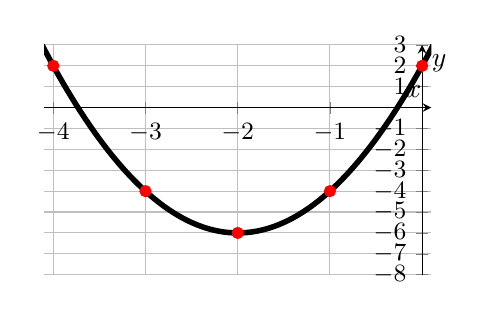
\begin{tikzpicture}[]
 		\begin{axis}[width=6.5cm,height=4.5cm, axis background/.style={fill=white}, axis lines=middle, 
 		grid = major,
 		xlabel=$\small x$,
 		ylabel=$\small y$, 
 		xtick={-5,-4,...,3},
 		ytick={-8,-7,...,3},
 		ymin = -8,
 		ymax = 3,
 		tick label style={font=\small},
 		legend style={font=\small,legend pos=outer north east},]
 		\addplot[ samples=201, line width=2pt]{2*x^2+8*x+2};
 		\addplot[red, mark=*, only marks] coordinates{(-4,2) (-3,-4) (-2,-6) (-1,-4) (0,2) };	
 		\end{axis}
 		\end{tikzpicture}
 	\end{minipage}
 \end{example}

\begin{mylist}
	

\exer  Calcula el vèrtex, l'eix de simetria i els punts d'intersecció amb els eixos de les següents paràboles. Dibuixa les seves gràfiques.

\begin{tasks}(2)
	\task  \textit{y =} \textit{x}${}^{2}$ + 8\textit{x} -- 13                          
	\task  \textit{y =} --\textit{x}${}^{2}$ + 8\textit{x} -- 13          
	\task  \textit{y =} \textit{x}${}^{2}$ -- 4\textit{x} + 2  
	\task  \textit{y =} \textit{x}${}^{2}$ + 6\textit{x                                  }
%	\task  \textit{y =} --\textit{x}${}^{2}$ + 4\textit{x} -- 7 \textit{}
\end{tasks}


\answers[cols=1]{[$V(-4,-29)$; talls $(-9.39,0)$ $(1.39,0)$ $(0,-13)$,
		  $V(4,3)$; talls $(2.27,0)$ $(5.73,0)$ $(0,-13)$,
		  $V(2,-2)$; talls $(0.59,0)$ $(3.41,0)$ $(0,2)$,
		  $V(-3,-9)$; talls $(-6,0)$ $(0,0)$ ]}


\exer \spen Completa aquest resum. En la gràfica de $y = ax^{2}$:
\begin{tasks} 
\task Si  $a > 0$ llavors té curvatura \quad \textsc{còncava} / \textsc{convexa}.
%
\task  Si $a > 1$ llavors té una obertura \quad \textsc{menor} / \textsc{major} \quad que $y=x^{2}$.
%
\task Si  $a < 0$ llavors té curvatura \quad \textsc{còncava} / \textsc{convexa}.
%
\task Si $-1<a<0$ llavors té una obertura \quad \textsc{menor} / \textsc{major} \quad que $y=x^{2}$.
\end{tasks}

\answers{[còncava, menor, convexa, major]}

	\vspace{-2.5cm}
\exer  \begin{minipage}[t]{0.65\textwidth}
	El pont \textit{Golden Gate} permet la comunicació entre els dos costats de la badia de San Francisco. Les seves torres, de 746~peus d'altura, estan separades per una distància d'uns 4200 peus. La calçada, que té una amplada de 90 peus i es troba a una altura de 220 peus sobre el nivell de l'aigua, està subjecta a les torres mitjançant dos cables, de 3 peus de diàmetre, que tenen forma de \textbf{paràbola} i que toquen la calçada en el centre del pont. 
\end{minipage}
\begin{minipage}{0.25\textwidth}
	\vspace{2.5cm}
	\raggedright
	\includegraphics*[width=1.1\textwidth]{img-08/goldenbridge}
\end{minipage}

\begin{tasks} 
%	\task  Realitza un dibuix on quedin reflectits les dades més significatives del problema.
	\task  Determina la relació que existeix entre l'altura a la qual es troba un punt del cable i la distància de la seva projecció vertical al  centre del pont. 
	\task  Aplica aquesta fórmula per calcular l'altura d'un punt del cable que la seva vertical està a 1000 peus del centre del pont.
\end{tasks}

\answers{[Respecte el centre el pont $y=0.0001193 x^2$, 119.27 peus d'altura]}

\end{mylist}
 

\begin{mylist}
	
	\exer  Escriu l'equació d'una paràbola d'igual forma que \textit{y =} \textit{x}${}^{2}$, però traslladada 5 unitats en sentit horitzontal a la dreta i 3 unitats en sentit vertical cap amunt. Quines coordenades té el seu vèrtex?
	
	\answers{$y=(x-5)^2+3 = x^2-10x+28$. El nou vèrtex és $V(5,3)$.}
	
	\exer  Un rectangle té un perímetre de 100 cm. Si anomenam \textit{x} a la longitud d'un dels seus costats, escriu la fórmula que dóna l'àrea en funció de \textit{x} . Dibuixa la seva gràfica. Quin tipus de funció és?
	
	\answers{$A=-x^2+50x$. És una funció quadràtica que talla a l'eix de les abscisses a $x=0$ i $x=50$ i vèrtex $V(25, 625)$ } 
	
	\exer  Una caixa quadrada té una altura de 20 cm. Com depèn el seu volum del costat de la base? Dibuixa la gràfica de la funció que resulta.
	
	\answers{$V=20x^2$}
	
	\exer  Amb un full de paper de 32 cm de llarg i 22 cm d'ample es retalla un quadrat de 2 cm de costat en cadascuna de les cantonades, es doblega i es construeix una caixa. Quin és el volum de la caixa? I si es retallen quadrats de 3 cm? Quin és el volum si el costat del quadrat retallat és\textit{ x}? Escriu la fórmula i dibuixa la gràfica.

\answers{$V = (32 – 2x) \cdot (22 – 2x)\cdot x$; $V(3) = 1248$ cm$^3$; $V(2) = 1 008$ cm$^3$}





\end{mylist}
 


\section{Interpretació i característiques de les funcions}


\begin{mylist}
	
	\exer  Assenyala totes les característiques que puguis de les funcions representades mitjançant les seves gràfiques: domini i recorregut, simetria, punts d'intersecció amb els eixos de coordenades, continuïtat, creixement i decreixement, màxims i mínims, periodicitat.
\begin{center}
\begin{tabular}{|c|c|} \hline 
 \rowcolor{lightgray}	GRÀFICA 1 & GRÀFICA 2 \\ \hline
	{\includegraphics[width=0.35\textwidth]{img-08/graf1}} & {\includegraphics[width=0.35\textwidth]{img-08/graf2}} \\ \hline
	\rowcolor{lightgray} GRÀFICA 3 & GRÀFICA 4 \\ \hline 
	 {\includegraphics[width=0.35\textwidth]{img-08/graf3}} & {\includegraphics[width=0.35\textwidth]{img-08/graf4}} \\ \hline 
\end{tabular}
\end{center}

\answers[cols=1]{[Gràfica 1: Dom $f=\Re$; Rec $f=[1,+\infty]$; Simetria parell; Talla eix OY a (0,1); És contínua; És decreixent $(-\infy,0)$ i creixent de $(0,+\infty)$; Té un mínim a (0,1),
		Gràfica 2: Dom $f=\Re$; Rec $f=\Re$; Simetria senar; Talla eix OX (--2,0) (0,0) (2,0) i l'eix OY a (0,0); És contínua; És decreixent $(-1,1)$ i creixent de $(-\infty,-1)\cup(1,+\infty)$; Té un màxim a (-1,3) i un mínim a (1,-3),
		Gràfica 3: Dom $f=\Re$-{0}; Rec $f=\Re-{0}$; Simetria senar; No hi ha talls amb eixos; No és contínua a x=0; Sempre decreixent; No té extrems,
		Gràfica 4: Dom $f=\Re$; Rec $f=[-1,1]$; Simetria senar; Talla l'eix OX a cada nombre enter; És contínua; És periòdica amb període 2. Presenta màxims a $0.5+2n$ i mínims $1.5+2n$ 
		]}


\exer  Joaquim ha arribat a un acord amb el seu pare per rebre la seva paga. Cobrarà 20~€ al mes el primer any, i 5~€ més per cada any que passi. Quant li correspondrà dins de 7 anys? Fes una taula de valors i representa la seva gràfica. És contínua? Indica els punts de discontinuïtat i el seu tipus. Busca una fórmula que permeti calcular la paga quan hagin passat \textit{n} anys.

\answers{
	D'aquí a 7 anys cobrarà 50 euros. És una funció esglaonada, ja que cobra el mateix durant tot un any, i després augmenta 5 euros:\par  $P =\left\{ \begin{array}{cl} 20 & \text{1r any} \\
	25 & \text{2n any} \\ 30 & \text{3r any} \\ \cdots & \\ 20 + 5(n-1) & \text{any }n  \end{array} \right.$}

	\exer  
	El consum de benzina i gasoil d'un cotxe per cada 100 km ve representat mitjançant la gràfica.
	
	\begin{minipage}{0.4\textwidth}
		\centering
		\includegraphics[height=4.5cm]{img-08/consumo}
	\end{minipage}
	\begin{minipage}{0.55\textwidth}
	\begin{tasks}(1)
		\task  Quina és la variable depenent? 
		\task  I la independent?
		\task  Quin és el consum per a una velocitat de 160 km/h?
		\task  A quina velocitat el consum és de 7 l/100 km?
		\task  Utilitza la gràfica per explicar com vària el consum de combustible depenent de la velocitat del cotxe.
	\end{tasks}
	\end{minipage}

\answers[cols=1]{[El consum en litres/100 km, La velocitat en km/h, Gasoil: 9.50 l/100 km; Benzina: 13 l/100 km, Gasoil: 135 km/h; Benzina: 105 km/h, El consum en general augment amb la velocitat i sempre és major el consum de benzina que no pas el de Gasoil.]}
  
 \exer La següent gràfica resumeix l'excursió que hem realitzat per la serra de Tramuntana:
		
	\begin{minipage}{0.4\textwidth}
		\centering
		\includegraphics[width=6.2cm]{img-08/graf45}
	\end{minipage}
	\begin{minipage}{0.53\textwidth}
	\begin{tasks}
		\task Quant temps va durar l'excursió?
		\task  Quant temps es va descansar? A quines hores?
		\task  Quants quilòmetres es van recórrer?
		\task  En quins intervals de temps es va anar més ràpid que entre les 11 i les 13 hores?
		\task  Fes una breu descripció del desenvolupament de l'excursió.
		%\task  Construeix una taula de valors a partir dels punts assenyalats en la gràfica.
		%\task  Si en l'eix d'ordenades representéssim la variable ``distància al punt de partida'', seria la mateixa gràfica? Amb les dades que disposes, pots fer-la?
	\end{tasks}
	
\end{minipage}

\answers[cols=1]{[12 hores, 3 hores de descans: entre les 14 i les 15 i entre les 18 i les 19 hores, Es van recórrer 80 km, En tots els altres excepte quan descansaven, lliure]} 

\exer  Durant un viatge, la velocitat del cotxe varia depenent del tipus de carretera, de les condicions en què es troba, del temps meteorològic{\dots} La següent gràfica reflecteix la velocitat d'un vehicle en cada instant del trajecte que ha seguit.
 
 
	\begin{minipage}{0.5\textwidth}
	\begin{tasks}
	\task  És funcional la relació de dependència entre el temps i la velocitat?
	\task  Quina és la variable independent? I la depenent?
	\task  A quina velocitat anava quan duia una hora de viatge? En quins moments anava a una velocitat de 40 km/h?
		\task  Indica els intervals en els quals la velocitat ha augmentat i disminuït. Ha estat constant en algun moment? Quan? Durant quant de temps?
	\end{tasks}
	\end{minipage}
	\begin{minipage}{0.5\textwidth}
		\centering
		\includegraphics[width=6.5cm]{img-08/graf43.pdf}
	\end{minipage}
\begin{tasks}
	\task[e)]  Quins són els màxims i mínims relatius de la funció? 
\end{tasks}

 
 \answers[cols=1]{[Sí. Es funcional, Independent: temps; Dependent: Velocitat, Anava a 90 km/h; Anava a 40 km/h als 20 i 110 minuts, Creixent $(0,40)\cup (50,70)$; Decreixent $(40,50)\cup (70,80)\cup (100,120)$; Constant: $(80,100)$ durant 20 minuts, 
 	Els màxims relatius són (40,80) i (70,120); El mínim relatiu és (50,60). ]} 
 
\vspace{-1.75cm}
\exer \begin{minipage}[t]{0.7\textwidth}
	 Una ciutat té implantada l'ordenança de regulació de l'aparcament (ORA). La norma indica que s'ha de pagar una certa quantitat per cada minut d'aparcament i que hi ha d'haver un mínim de preu. En Joan posa 1,35 \euro{} i el parquímetre indica que disposa de 45 minuts. Sara amb 0,84 \euro{} només té 28 minuts.

\end{minipage}
\begin{minipage}{0.3\textwidth}
	\centering
	\vspace{1.5cm}
	\includegraphics[width=0.5\textwidth]{img-08/ora}
\end{minipage}
	\begin{tasks}(1)
	\task Troba l'equació de la funció lineal $y=mx+n$ que relaciona el temps $x$ amb el preu $y$.
	\task Quant hem de pagar per un aparcament de 55 minuts?	
	\task Si hem pagam 2,40 \euro{} de quant de temps disposam?
\end{tasks}
 
\answers[cols=1]{[$y=0.03 x$, $1.65$ \euro{}, 80 minuts]}
 

\exer  En estudiar el creixement d'una planta observem que durant els primers 30 dies ho fa molt de pressa, en els 15 dies següents el creixement és més lent i després es manté amb la mateixa altura. Realitza un esbós de la gràfica que relaciona el temps amb l'altura aconseguida per la planta.


 Si tenim més informació podem millorar l'esbós. Per exemple, fes la taula i la gràfica en el cas que el creixement de la planta s'ajusti a les següents fórmules (el temps s'expressa en dies i l'altura en centímetres):
\begin{tasks}(1)
\task  Durant els primers 30 dies:  altura = 4 $\cdot$ temps
\task En els dies 30 a 45: altura = 90 + temps
 \end{tasks}

\answers{Gràfica: \par \includegraphics[width=0.45\textwidth]{img-sol/t8-45}}

\begin{comment}
\exer  Un viatge realitzat per un tren, en un cert interval de temps, ve donat de la següent forma:
\begin{itemize}
 \exer Durant les dues primeres hores, la distancia ``$d$'' (en quilòmetres) al punt de partida és $2t+1$, on ``$t$'' és el temps (en hores) de durada del trajecte.

 \exer Entre la 2a i 3a hora, aquesta distància ve donada per $-t+7$.

 \exer Entre la 3a i 4a hora, ambdues inclusivament, $d=4$.

 \exer Des de la 4a i fins a la 6a (inclusivament), la distància s'ajusta a $3t-8$.
\end{itemize}

Realitza una taula i una gràfica que reculli aquest viatge de la forma més precisa possible (per a això has de calcular, com a mínim, els valors de la variable temps en els instants 0, 2, 3, 4 i 6).
\begin{tasks}(1)
   \task Explica si la relació anteriorment explicada entre la distància recorreguda i el temps trigat a recórrer-la és funcional.
   \task La relació anterior, presenta alguna discontinuïtat?
   \task En quin moment la distància al punt de partida és de 7 km?
   \task Què indiquen els punts de tall de la gràfica amb els eixos?
   \task Determina els intervals on la funció és creixent, decreixent i constant.
   \task Troba els punts on la funció assoleix els seus màxims i mínims relatius i absoluts. Interpreta el significat que puguin tenir.
\end{tasks}



\exer  Representa gràficament les següents funcions, estudiant en ella totes les característiques que s'han treballat en el tema: monotonia, extrems, simetria i periodicitat.
\begin{tasks}(1)
  \task Valor absolut d'un nombre: $f\left(x\right)=\left|x\right|$.
   \task Oposat i invers d'un nombre: $f\left(x\right)=\frac{-1}{x} $.
   \task \textit{Mantissa} (a cada nombre li correspon la diferència entre aquest nombre i la seva part enter
  : $M\left(x\right)=x-E\left(x\right)$.
\end{tasks}


\exer  Les gràfiques següents mostren l'evolució, un dia qualsevol, de la temperatura aconseguida entre les 7 del matí i les 4 de la tarda en quatre ciutats (Madrid, Granada, Valladolid i Sevilla):


\begin{longtable}{|p{0.24\textwidth}|p{0.24\textwidth}|p{0.24\textwidth}|p{0.24\textwidth}|} \hline 
\includegraphics[width=0.2\textwidth]{img-08/image13.png} & \includegraphics*[width=0.2\textwidth]{img-08/image14.png} & \includegraphics*[width=0.2\textwidth]{img-08/image15.png} & \includegraphics*[width=0.2\textwidth]{img-08/image16.png} \\ \hline 
\end{longtable}

\begin{tasks}
\task  Estudia la monotonia de totes les gràfiques.
\task   En alguna ciutat la temperatura s'ha mantingut constant durant tot l'interval? I en part d'ell?
\task   Quina ciutat creus que presenta un canvi de temperatura més suau al llarg de tot el matí?
\task   Tenint en compte que a Madrid l'increment de la temperatura ha estat sempre lineal, a Granada la temperatura mínima s'ha aconseguit després de les 7 h i a Valladolid a partir del mig dia la temperatura va baixar, indica quina gràfica correspon a cadascuna de les ciutats i explica quins han estat les temperatures màximes i mínimes en cadascuna d'elles.
\end{tasks}
\end{comment}
\end{mylist}


\begin{autoaval}{38}
\begin{mylist}

 
\exer[2] L'únic punt que té ordenada negativa i es troba al 3r quadrant és:
\begin{tasks}(4)
\task $(-1,1)$
\task $(-1,-1)$
\task $(-1,0)$
\task $(1,-1)$
\end{tasks}  
\answers{\textbf{--6.} Autoavaluació: 1b; 2d; 3a; 4c; 5b; 6b}

\exer L'única taula que no correspon a una relació funcional és:
\begin{tasks}(4)
\task \begin{tabular}{|c|c|}
	\hline
	\rowcolor{lightgray} $x$ & $y$ \\
	\hline
 	0 & 1 \\ 
	\hline 
	1 & 2 \\ 
	\hline 
	2 & 3 \\ 
	\hline 
	3 & 4 \\ 
	\hline 
\end{tabular} 
\task  \begin{tabular}{|c|c|}
	\hline
	\rowcolor{lightgray} $x$ & $y$ \\
	\hline
	0 & 1 \\ 
	\hline 
	1 & 1 \\ 
	\hline 
	2 & 1 \\ 
	\hline 
	3 & 1 \\ 
	\hline 
\end{tabular} 
\task  \begin{tabular}{|c|c|}
	\hline
	\rowcolor{lightgray} $x$ & $y$ \\
	\hline
	0 & --1 \\ 
	\hline 
	1 & --1 \\ 
	\hline 
	2 & --2 \\ 
	\hline 
	3 & --3 \\ 
	\hline 
\end{tabular} 
\task  \begin{tabular}{|c|c|}
	\hline
	\rowcolor{lightgray} $x$ & $y$ \\
	\hline
	0 & 0 \\ 
	\hline 
	1 & 1 \\ 
	\hline 
	2 & 2 \\ 
	\hline 
	0 & --3 \\ 
	\hline 
\end{tabular}  
\end{tasks}

  
 
\exer  L'única funció afí que passa per l'origen de coordenades és 
\begin{tasks}(4)
\task $y = -4x$
\task $y = 3x + 1 $
\task $y = -2x + 3$
\task $y = -x - 1$
\end{tasks}

\exer L'única funció quadràtica és:
\begin{tasks}(4)
\task $y = -2x$
\task $y = 3x + 1 $
\task $y = -2x^2 + 3x$
\task $y = -x^3 - 1$
\end{tasks}
 

\exer La funció quadràtica que té el seu vèrtex en el punt (3, 9) és:
\begin{tasks}(4)
	\task $y = -2x^{2}$
	\task $y = -x^{2} +6x$
	\task $y = 3x^{2}-x + 1$
	\task $y = -2x^{2} + 3x$
\end{tasks}
 
\exer La única funció que és periòdica és:
\begin{tasks}(4)
	\task
	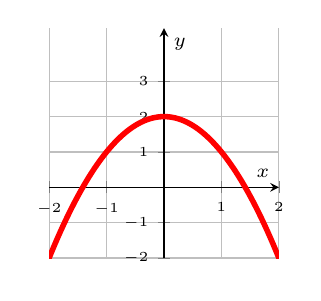
\begin{tikzpicture}[]
	\begin{axis}[width=4.5cm,height=4.5cm, axis background/.style={fill=white}, axis lines=middle, 
	grid = major,
	xlabel=$\scriptstyle x$,
	ylabel=$\scriptstyle y$, 
	xtick={-3,-2,...,5},
	ytick={-3,-2,...,3},
	ymin = -2,
	ymax = 4.5,
	tick label style={font=\tiny},
	legend style={font=\footnotesize,legend pos=outer north east},]
	\addplot[red, samples=201, line width=2pt]{-x^2+2};	
	\end{axis}
	\end{tikzpicture}
	\task 	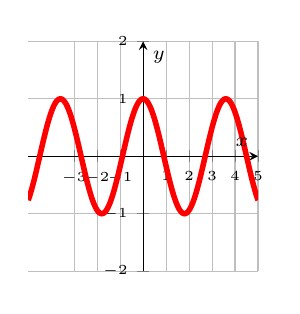
\begin{tikzpicture}[]
	\begin{axis}[width=4.5cm,height=4.5cm, axis background/.style={fill=white}, axis lines=middle, 
	grid = major,
	xlabel=$\scriptstyle x$,
	ylabel=$\scriptstyle y$, 
	xtick={-3,-2,...,5},
	ytick={-2,-1,...,2},
	ymin = -2,
	ymax = 2,
	tick label style={font=\tiny},
	legend style={font=\footnotesize,legend pos=outer north east},]
	\addplot[red, samples=201, line width=2pt]{cos(100*x)};	
	\end{axis}
	\end{tikzpicture}
	\task 	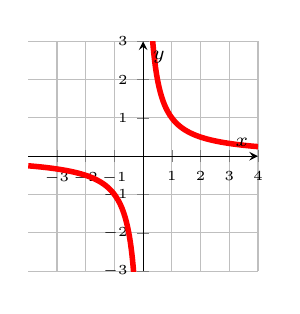
\begin{tikzpicture}[]
	\begin{axis}[width=4.5cm,height=4.5cm, axis background/.style={fill=white}, axis lines=middle, 
	grid = major,
	xlabel=$\scriptstyle x$,
	ylabel=$\scriptstyle y$, 
	xtick={-3,-2,...,5},
	ytick={-3,-2,...,3},
	ymin = -3,
	ymax = 3,
	tick label style={font=\tiny},
	legend style={font=\footnotesize,legend pos=outer north east},]
	\addplot[red, domain=-4:-0.01, samples=201, line width=2pt]{1/x};
	\addplot[red, domain=0.01:4, samples=201, line width=2pt]{1/x};		
	\end{axis}
	\end{tikzpicture}
	\task 	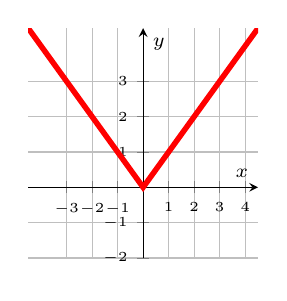
\begin{tikzpicture}[]
	\begin{axis}[width=4.5cm,height=4.5cm, axis background/.style={fill=white}, axis lines=middle, 
	grid = major,
	xlabel=$\scriptstyle x$,
	ylabel=$\scriptstyle y$, 
	xtick={-3,-2,...,5},
	ytick={-3,-2,...,3},
	ymin = -2,
	ymax = 4.5,
	tick label style={font=\tiny},
	legend style={font=\footnotesize,legend pos=outer north east},]
	\addplot[red, samples=201, line width=2pt]{abs(x)};	
	\end{axis}
	\end{tikzpicture}
\end{tasks}

 
\end{mylist}
\end{autoaval}

\newpage

\begin{extrapage}
	\heading{Taxi}

	Un taxi cobra una quantitat fixa per pujar-hi i 1,50\euro el quilòmetre recorregut. Sabem que ens ha
	costat 16,50\euro per fer un viatge de 10 km.

	\begin{tasks}(1)
		\task Escriu la funció que expressa el preu del viatge segons els quilòmetres recorreguts. 
			 Representau-la gràficament.
		\task Quin és el preu fix per pujar al taxi?
		\task Si feim un recorregut de 7 km, quant hem de pagar?
		\task Si disposam de 30 \euro dins la butxaca, quin és el desplaçament màxim podem realitzar?
	\end{tasks}

	\vspace{0.5cm}

	\heading{Reserva d'hotel}
	
	L'agència \textit{Bon Viatge}  ofereix un paquet de 7 dies d'allotjament per a dues persones a 
	l'\textit{hotel la Sirena} per 3500\euro, amb l'opció d'allargar l'estada fins un màxim de 10 dies 
	pagant un plus de 600 \euro per dia.
	
	Un altre operador turístic, \textit{Travelindo}, ofereix allotjament en el mateix hotel, 
	també per a dues persones per 530\euro dia, per un mínim de 4 dies d'allotjament.

	Una altra opció és contractar directament amb l'hotel, el qual ofereix una tarifa de 600\euro dia sense 
	restriccions de temps d'estada.

	\begin{tasks}(1)
		\task Si es pensa passar 8 dies a l'hotel, quina agència convé contractar?
		\task Si es pensa passar només 3 dies, quina opció convé més?
		\task Si disposam de 15 dies de vacances, quina agència convé?
		\task Quina és la forma més eficaç de representar la informació per decidir sobre
			  l'opció millor en cada cas? Generalitza les respostes anteriors per un nombre 
			  indeterminat de dies $x$.

		\task Hi ha algun nombre de dies pel qual les diferents opcions siguin equivalents? 
	\end{tasks}

	\vspace{0.5cm}

	\heading{Impressió de llibres}
	
	En Manel vol imprimir la seva novel·la i demana pressupost a una imprenta. Li diuen que el cost 
	d'impressió per cada llibre seria:
	
	\begin{itemize}
		\item \textbf{5,50 \euro / llibre} si decideix imprimir de 0 a 100 llibres.
		\item \textbf{5,00 \euro / llibre} si decideix imprimir una quantitat superior a 100 i inferior a 300 llibres.
		\item \textbf{4,50 \euro / llibre} si imprimeix una quantitat superior a 300 llibres.
	\end{itemize}
	
	\begin{tasks}(1)
		\task Quant ha de pagar en Manel si imprimeix 60 llibres? I si n'imprimeix 220? I 400?
		\task Representau la gràfica de la funció que proporciona el cost d'impressió segons el nombre de llibres.
		\task Calcula les equacions de les rectes que apareixen a l'apartat b).
		\task Si sabem que en Manel va pagar 850\euro, quants de llibres va decidir imprimir?
	\end{tasks}


\end{extrapage}
 
\newpage
\resum
\begin{center}
	\renewcommand{\arraystretch}{1.5}
\begin{longtable}{|p{0.2\textwidth}|p{0.35\textwidth}|p{0.3\textwidth}|} 
	\hline 
	\cellcolor{lightgray}\textbf{Punts}
	 & \vspace{-0.25cm}
	 \begin{center}\includegraphics[width=0.32\textwidth]{img-08/image23.png}\end{center}\vspace{-0.25cm} & \vspace{-0.25cm} \begin{center}\includegraphics[width=0.32\textwidth]{img-08/image24.png}\end{center} \vspace{-0.25cm} \\ \hline
	 
	\rowcolor{lightgray} \multicolumn{3}{|p{\textwidth}|}{\textbf{Funció}} \\ \hline
 	 
\multicolumn{2}{|p{0.55\textwidth}|}{ Una \textbf{funció }és una relació entre dues magnituds de manera que a un valor qualsevol d'una (\textbf{variable independent}) li fem correspondre, com a molt, un únic valor de l'altra (\textbf{variable depenent}).} & 
\newline

$\begin{array}{l} {y=f\left(x\right)=0,59\, \cdot \, x} \\ {f\left(2\right)=0,59\, \cdot \, 2=1,18} \\ {f\left(5\right)=0,59\, \cdot \, 5=2,95} \end{array}$ \\ \hline 

	\rowcolor{lightgray} \multicolumn{3}{|p{\textwidth}|}{\textbf{Gràfica d'una funció}} \\ \hline

\multicolumn{2}{|p{0.55\textwidth}|}{ La \textbf{gràfica d'una funció }és la representació en el pla cartesià de tots els parells ordenats en els quals el primer valor correspon a un qualsevol de la variable independent i el segon al que s'obté en transformar-ho mitjançant la funció:\newline $\{$(\textit{x}, \textit{y}) $\in$ \textbf{$\Re$}, \textit{y =} \textit{f}(\textit{x})$\}$} & 
\textit{Gràfica: } 

\begin{center}
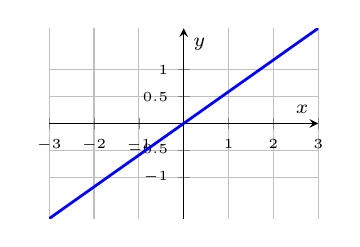
\begin{tikzpicture}[]
\begin{axis}[width=5cm,height=4cm, axis background/.style={fill=white}, axis lines=middle, 
 grid = major,
xlabel=$\scriptstyle x$,
ylabel=$\scriptstyle y$, 
xtick={-3,-2,...,3},
ytick={-1,-0.5,...,1},
tick label style={font=\tiny},
legend style={font=\footnotesize,legend pos=outer north east},]
\addplot[blue,domain=-3:3,samples=201, line width=1pt]{.59*x};	
\end{axis}
\end{tikzpicture}

$y=f(x)=0,59 x$
\end{center}
\\ \hline 

	\rowcolor{lightgray} \multicolumn{3}{|p{\textwidth}|}{\textbf{Funció afí, funció lineal i funció constant}} \\ \hline
	
 \multicolumn{2}{|p{0.55\textwidth}|}{
Una \textbf{funció afí} és aquella funció en la qual la relació entre les dues variables ve donada per un polinomi de grau menor o igual a 1: 
\[y=mx+n\]
La representació gràfica és una recta. 

``\textit{m}''\textit{ }rep el nom de \textbf{pendent} i ``\textit{n}''\textit{ }\textbf{ordenada a l'origen.}

Una \textbf{funció lineal } o \textbf{ de proporcionalitat directa} és una funció afí amb ordenada en l'origen nul·la: \textit{y = mx }(passa per l'origen).


Una \textbf{funció constant }és una funció afí amb pendent nul: \textit{y = n} (sempre pren el mateix valor i la seva gràfica és una recta horitzontal).} &
\begin{center}
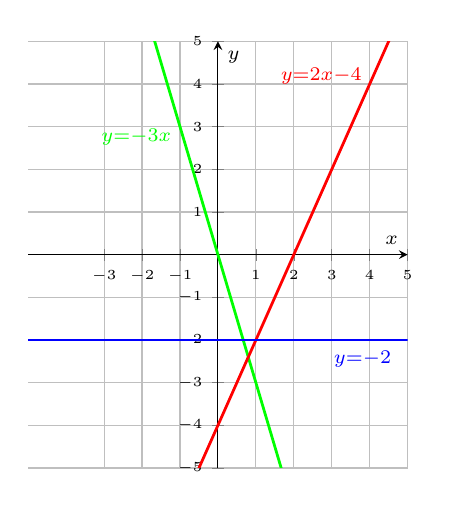
\begin{tikzpicture}
\begin{axis}[width=6.4cm,height=7cm, axis background/.style={fill=white}, axis lines=middle, 
 grid = major,
xlabel=$\scriptstyle x$,
ylabel=$\scriptstyle y$, 
xtick={-3,-2,...,5},
ytick={-5,-4,...,5},
ymin = -5,
ymax = 5,
tick label style={font=\tiny},
legend style={font=\footnotesize,legend pos=outer north east},]
\addplot[green, domain=-2:2, samples=201, line width=1pt]{-3*x} node[above, pos=1, xshift=-2cm, yshift=4.5cm] {$\scriptstyle y=-3x$};
\addplot[red, samples=201, line width=1pt]{2*x-4} node[anchor=north east,yshift=-0.75cm, xshift=-0.45cm] {$\scriptstyle y=2x-4$};
\addplot[blue, samples=201, line width=1pt]{-2} node[anchor=north east,xshift=-0.075cm] {$\scriptstyle y=-2$};	
\end{axis}
\end{tikzpicture}
\end{center}
 \\ \hline 
 
 \end{longtable}

 \pagebreak
 
 \renewcommand{\arraystretch}{2.5}
 \begin{longtable}{|p{0.2\textwidth}|p{0.35\textwidth}|p{0.3\textwidth}|} 
 	\hline 
 	\rowcolor{lightgray} \multicolumn{3}{|p{\textwidth}|}{\textbf{Funció quadràtica}} \\ \hline
 
  \multicolumn{2}{|p{0.55\textwidth}|}{Una funció quadràtica és aquella funció en la qual la relació entre les dues variables ve donada per un polinomi de grau dos:
\[y=f(x)=a x^2+b x + c\]
La gràfica d'aquest tipus de funcions es diu paràbola.

 El punt més significatiu de la paràbola és el \textbf{vèrtex} i es calcula donant-li a la variable independent el valor $x_v= -b/2a$
 
  Si el coeficient de $x^{ 2}$ és positiu, el vèrtex és un mínim i, si és negatiu, un màxim.} & 
\begin{center}
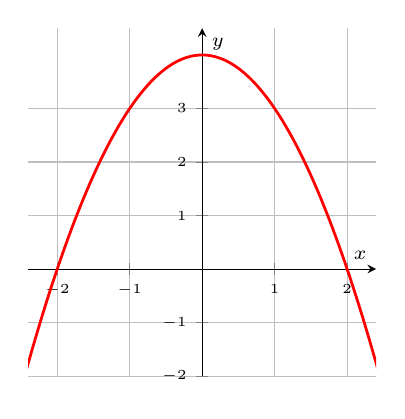
\begin{tikzpicture}[]
\begin{axis}[width=6cm,height=6cm, axis background/.style={fill=white}, axis lines=middle, 
 grid = major,
xlabel=$\scriptstyle x$,
ylabel=$\scriptstyle y$, 
xtick={-3,-2,...,5},
ytick={-3,-2,...,3},
ymin = -2,
ymax = 4.5,
tick label style={font=\tiny},
legend style={font=\footnotesize,legend pos=outer north east},]
\addplot[red, samples=201, line width=1pt]{4-x^2};	
\end{axis}
\end{tikzpicture}

$y=4-x^2$
\end{center}
 \\ 
\hline 

	\rowcolor{lightgray} \multicolumn{3}{|p{\textwidth}|}{\textbf{Continuïtat, Monotonia, Extrems, Simetria  i Periodicitat}} \\ \hline
 
  \multicolumn{2}{|p{0.55\textwidth}|}{
  Una funció pot ser:
  
  \begin{itemize}
   \item contínua en un interval si la seva gràfica no sofreix ``ruptures'' (anomenades \textbf{discontinuïtats})
   
   \item \textbf{creixent }(\textbf{decreixent}) si el seu valor augmenta (disminueix) quan ho fa la variable independent
   
   \item \textbf{constant }quan sempre pren el mateix valor
   
   \item \textbf{parell} si la imatge de la variable independent coincideix amb el del seu oposat, \textbf{imparell} quan el valor de la funció per a l'oposat de la variable independent també és l'oposat 
   
   \item \textbf{periòdica} si les imatges dels valors obtinguts en sumar una quantitat fixa (\textbf{període}) a la variable independent coincideixen.
\end{itemize}
} &
\begin{center} \includegraphics*[width=0.4\textwidth]{img-08/image28.png}
\end{center}\\ \hline 
\end{longtable}
\end{center}




\mychapter{Geometria en el pla}{Geometria en el pla}{\begin{center}\includegraphics[width=0.9\textwidth]{img-09/pitagoras} \footnotesize Demostració del teorema de Pitàgores\end{center}}{chap:geo2d}

\begin{iniaval}
	
    \begin{minipage}{0.6\textwidth}
			Hem anat a la copisteria i hem fet una fotocòpia ampliada del logo del nostre centre.
			
			\begin{tasks}
			 \task Quina ampliació ens han fet?
			 \task Què valdran les mesures que falten?
			 \task Què val l'àrea del cercle ampliat?
			 \end{tasks}
	\end{minipage}
	\begin{minipage}{0.4\textwidth}
		\centering
			\includegraphics[width=\textwidth]{img-09/ampliacio1}
	\end{minipage}
	 
	 \vso\vso
	
	 \begin{minipage}{0.65\textwidth}
	  d) A casa, estam dissenyant un logo similar amb les mides que apareixen en la figura. Ens agradaria saber quina quantitat de cartolina necessitam per poder fer la figura.  Ens ajudes?

	 \end{minipage}
	 \begin{minipage}{0.35\textwidth}
	 	\centering
	 	\includegraphics[width=0.9\textwidth]{img-09/ampliacio2}
	 \end{minipage}
	 \vsoo
	 
	 \addanswersline[cols=1]{Avaluació inicial}{0}{[La raó és $r=\dfrac{3}{2}=1.5$. Han ampliat un 150 \%, Les mesures són 1.5 cm i 6 cm, L'àrea del cercle ampliat és 7.1 cm$^2$, $A=1079$ cm$^2$.]}
\end{iniaval}

\newpage
\section{Semblança}

\begin{theorybox}
	\begin{wrapfigure}{R}{0.3\textwidth}
		\centering
			\includegraphics[width=0.28\textwidth]{img-09/trig-semblant}
	\end{wrapfigure}
	
	Dues figures són semblants si són una còpia ampliada o reduïda una de l'altre (sense deformar-la). 
	
	Dues figures semblants \textbf{conserven tots els angles}. Els seus costats són tots proporcionals i la constant de proporcionalitat s'anomena \textbf{raó de la semblança} $r$.
	
	\textbf{Teorema de Tales}: Dos triangles $ABC$ i $A'B'C'$ són semblants si: 
	
	\begin{itemize}
		\item Té dos angles iguals $\hat A = \hat A'$  i $\hat B = \hat B'$ o
		\item Els seus costats són proporcionals $\frac{a}{a'}=\frac{b}{b'}=\frac{c}{c'}=r$
	\end{itemize}
	

\end{theorybox}

\begin{mylist}
\exer  Indica si són semblants els següents parells de triangles:



\begin{tasks}
	\task  Un angle de 80${}^\circ$  i un altre de 40${}^\circ$ . Un angle de 80${}^\circ$  i un altre de 60${}^\circ$ . 
	\task  Triangle isòsceles amb angle desigual de 70${}^\circ$ . Triangle isòsceles amb angle igual de 50${}^\circ$ .
	\task  \textit{A =} 30${}^\circ$ , \textit{b} = 7 cm, \textit{c} = 9 cm. \textit{A'}= 30${}^\circ$ , \textit{b}' = 3.5 cm, \textit{c}' = 4.5 cm
	\task  \textit{a =} 4 cm, \textit{b} = 5 cm, \textit{c} = 7 cm. \textit{a'} = 10 cm, \textit{b'} = 12.5 cm, \textit{c'} = 24.5 cm
\end{tasks}

\answers[cols=1]{[Sí perquè tenen tots els angles iguals, 
	No perquè els seus angles respectius són 70; 55; 55 i 80; 50; 50,
 	Si perquè tenen un angle igual i els costats que els formen són proporcionals (la meitat).
	No perquè $\dfrac{a'}{a} = \dfrac{b'}{b} = 2.5$ però $\dfrac{c'}{c} = 3.5$]}


\exer  Calcula el valor desconegut perquè els triangles siguin semblants:

\begin{tasks}
	\task  \textit{a =} 9 cm, \textit{b} = 6 cm, \textit{c} = 12 cm. \textit{a}' = 6 cm, \textit{b'} = 4 cm, \textit{c'=}?
	\task  \textit{A =} 45${}^\circ$ , \textit{b} = 8 cm, c = 4 cm. \textit{A'} = 45${}^\circ$ , \textit{b'} = 8 cm, \textit{a'=}?
\end{tasks}

\answers{[$c'=8$ cm, $c'=8$ cm]}

\exer  Na Maria mesura 160~cm i la seva ombra mesura 90~cm. En aquest mateix instant es mesura l'ombra d'un edifici i mesura 7,2~m. Quant mesura l'edifici?

\answers{L'edifici mesura 12.8 m.}

\exer  Un triangle té costats de 6 cm, 7 cm i 7 cm. Un triangle semblant a ell té un perímetre de 60 cm. Quant mesuren els seus costats?

\answers{Primer trobam la raó de semblança $\dfrac{60}{(6+7+7)}=3$. Els nous costats s'obtenen de multiplicar per 3 els originals: 18 cm, 21 cm i 21 cm}

\begin{resolt}[E]{
	Calcula $\overline{CD}$ i $\overline{BC}$ de la figura:
	
	\begin{center}
		\includegraphics[width=0.2\textwidth]{img-09/sampleTales}
	\end{center}	

sabent que  $\overline{AC}=15$ cm, $\overline{CE}=11$ cm, $\overline{BD}=6.4$ cm i $\overline{AE}=18$ cm.
}
		
		Aplicam que els triangles $\widehat{ACE}$ i $\widehat{BCD}$ són semblants i, per tant, tots els seus costats són proporcionals.
		
		\[ \frac{18}{6.4} = \frac{11}{\overline{CD}}  \quad \rightarrow \quad \overline{CD} = \frac{6.4 \cdot 11}{18} = 3.9 \text{ cm } \]
		
		\quad i
		
		
		\[ \frac{15}{\overline{BC}} = \frac{11}{\overline{3.9}}  \quad \rightarrow \quad \overline{BC} = \frac{15 \cdot 3.9}{11} = 5.3 \text{ cm } \]
\end{resolt}
\newpage

\exer[1]  Calcula els valors de  $x$ i $y$ en les següents figures. 

\begin{tasks}(2)
	\task   \includegraphics[width=0.3\textwidth]{img-09/trig-semblant2}
	\task    \includegraphics[width=0.35\textwidth]{img-09/trig-semblant5}
\end{tasks}
\answers[cols=1]{[$x=4$ i $y=3$ cm, $x=6$ i $y=18$ cm]}

\exer  Un pal alt es subjecta amb cables d'acer que van del seu extrem superior al sòl. La distància de l'ancoratge d'un dels cables a la base del pal és 6 metres. Posem una barra de 120 centímetres de manera que està perpendicular al sòl i just toca el sòl i el cable. La seva distància a l'ancoratge del cable és 90 centímetres. Calcula la longitud del pal i la longitud del cable d'acer.

 \answers{Esquema:\par \includegraphics[width=0.3\textwidth]{img-sol/t9-5}\par El pal mesura   8 m i el cable 10 m.}

\exer  Calcula les longituds que s'indiquen:
\begin{tasks}(2)
	\task    \includegraphics[width=0.35\textwidth]{img-09/trig-semblant3}
	\task   \includegraphics[width=0.4\textwidth]{img-09/trig-semblant4}
\end{tasks}

\answers[cols=1]{[$x=2$; $y=1.375$ cm,  $x=9$; $y=3$; $z=4.5$ cm]}

\end{mylist}
 


\section{Angles, longituds i àrees}

\begin{theorybox}
	Per qualsevol triangle, la suma dels seus angles és $\hat A + \hat B+ \hat C = 180^\circ$.
	
	\begin{minipage}{0.6\textwidth}
		Si un triangle té un angle de 90$^\circ$, \textbf{triangle rectangle}, podem aplicar el \textbf{teorema de Pitàgores}:
		\[a^2 = b^2 + c^2 \]
		on $a$ és la \textbf{hipotenusa} (el costat més llarg) i $b$ i $c$ els \textbf{catets}.
	\end{minipage}
\begin{minipage}{0.4\textwidth}
	\centering
	\includegraphics[width=0.8\textwidth]{img-09/pitagores}
\end{minipage}

Si sabem els catets, la hipotenusa s'obté de  $a=\sqrt{b^2+c^2}$.

Si ens falta un catet, aquest s'obté de $b=\sqrt{a^2-c^2}$  o $c=\sqrt{a^2-b^2}$ .
\end{theorybox}
 

\begin{mylist}
\exer  És possible trobar un triangle rectangle els catets del qual mesurin 5 i 12 cm i la seva hipotenusa 24 cm? Si la teva resposta és negativa, troba la mesura de la hipotenusa d'un triangle rectangle els catets del qual mesuren 5 i 12 cm. Utilitza calculadora per resoldre aquesta activitat si et resulta necessària. 

\answers{Sí. La hipotenusa ha de mesurar 13 cm}

\exer  Calcula la longitud de la hipotenusa dels següents triangles rectangles de catets:

\begin{tasks}(2)
	\task  6 cm i 8 cm   
	\task  4 m i 3 m
	\task  8 dm i 15 dm  
	\task  13,6 km i 21,4 km.
\end{tasks}
\answers[cols=2]{[10 cm, 5 m, 17 dm, 25.4 km]}

\exer  Calcula la longitud del catet que falta en els següents triangles rectangles d'hipotenusa i catet:

\begin{tasks}(2)
	\task  26 cm i 10 cm   
	\task  17 m i 8 m
	\task  37 dm i 35 dm  
	\task  14,7 km i 5,9 km
\end{tasks}
\answers[cols=2]{[24 cm,  15 m, 12 dm, 13.5 km]}

\exer[1] \hot  Calcula el costat $x$ del quadrat de la figura següent:
\begin{center}
 \includegraphics[width=0.2\textwidth]{img-09/fig6}
\end{center}
\answers{$x=8$ cm}

\end{mylist}
	
\begin{theorybox}[Fórmules àrees]	
	Trobareu un resum de les àrees de les figures planes a la pàgina \pageref{sec:resumarees}.
\end{theorybox}


\begin{mylist}

\exer  Calcula l'àrea d'un triangle equilàter de costat 9 m. 
\answers{$A=\frac{81}{4}\sqrt{3}=35.74$ cm$^2$.}

\exer  Calcula l'àrea d'un hexàgon regular de costat 2 cm. 
\answers{L'apotema és $a_p=1.732$. $A=6\sqrt{3}=10.39$ cm$^2$}

\exer  \hot Calcula el volum d'un tetraedre regular de costat 7 dm.
\answers{$V=\frac{1}{3}A_{base}H$. $A_{base}=21.218$, l'altura cau a 1/3 del costat la base $H=\frac{\sqrt{6}}{3}c=5.715$. $V=40.42$ dm$^3$}

\exer  Calcula la longitud de la diagonal d'un quadrat de costat 3 m.
\answers{$3\sqrt{2}=4.24$ m}

\exer  Calcula la longitud de la diagonal d'un rectangle de base 15 cm i altura 8 cm.
\answers{17 cm}

\exer  Una porteria de futbol mesura 7,32~m d'ample per 2,44~m d'alt. El punt de penal està a 10 metres. Calcula la distància que recorre la pilota en:

\begin{tasks}(2)
	\task  Un tir directe a la base del pal.

 
	\task  Un tir directe a l'esquadra.
\end{tasks}
\answers{[10.65 m, 10.92 m]}


\exer  Demostra que el diàmetre d'un quadrat de costat \textit{x} és $d=\sqrt{2} x$.
 

\exer  Demostra que l'altura d'un triangle equilàter de costat \textit{x} és $d=\frac{\sqrt{3} }{2} x$. 
 

\exer  Calcula els angles central i interior del triangle equilàter, quadrat, pentàgon regular, hexàgon regular i enneàgon regular.
\answers{120${}^\circ$ i 60${}^\circ$; 90${}^\circ$ i 90${}^\circ$; 72${}^\circ$ i 108${}^\circ$; 60${}^\circ$ i 120${}^\circ$; 40${}^\circ$ i 140${}^\circ$.}

\exer  Justifica que un hexàgon regular es pot descompondre en 6 triangles equilàters.
\answers{
	L'angle central mesura 60${}^\circ$. El triangle format per dos radis consecutius i el costat corresponent és
	isòsceles perquè tots els radis són iguals. L'angle suposadament desigual d'aquest triangle isòsceles
	mesura 60${}^\circ$ així que els altres dos angles també han de mesurar 60. Un triangle amb els tres angles iguals
	és equilàter.}

\exer  Dos angles d'un triangle isòsceles mesuren 35${}^\circ$  i 72${}^\circ$ , quant pot mesurar l'angle que falta?
\answers{Mesura 73${}^\circ$}

\exer  Dos angles d'un trapezi isòsceles mesuren 35${}^\circ$  i 72${}^\circ$ , quant mesuren els angles que falten?

\answers{En un trapezi isòsceles els angles són iguals dos a dos i han de ser dos aguts i dos obtusos persumar en total 360. Aquest trapezi no pot ser isòsceles.}

\exer  Quant mesura la suma dels angles interiors d'un decàgon irregular? 
\answers{Els angles interiors sumen 1440${}^\circ$.}

\exer  Calcula l'àrea i el perímetre d'un trapezi isòsceles de bases 50 cm i 26 cm i altura 5 cm.
\answers{Àrea: 190 cm$^2$; perímetre: 128 cm.}

\exer  Calcula l'àrea i perímetre d'un trapezi rectangle de bases 100~cm i 64~cm, i d'altura 77~cm.
\answers{Àrea: 574 cm$^2$; perímetre: 326 cm}
 
\exer  Calcula l'àrea i el perímetre d'un trapezi isòsceles de bases 100 cm i 60~cm i costats laterals 29~cm.
\answers{Àrea: 1 470 m$^2$; perímetre: 198 cm.}

\vspace{-1.5cm}
\exer[1] \begin{minipage}[t]{0.66\textwidth}
	 Utilitza el teorema de Pitàgores per determinar l'àrea i el perímetre de la zona ombrejada de la figura.
\end{minipage}
\begin{minipage}{0.3\textwidth}
	\centering
	\vspace{1.5cm}
\includegraphics[width=0.8\textwidth]{img-09/fig7}
\end{minipage}
 \answers{$A=4.5$ cm$^2$, $P=15.62$ cm}
 
\exer  Tenint en compte que un hexàgon regular es pot dividir en sis triangles equilàters (l'altura de la qual és l'apotema de l'hexàgon regular), calcula l'àrea d'un hexàgon regular de 5 cm de costat.
\answers{El radi també és 5 cm i l'apotema $a_p=4.33$. L'àrea és: 64.95 cm$^2$}

\exer  Volem cobrir el pla amb polígons regulars de 100 cm${}^{2}$. Les úniques opcions possibles són el triangle equilàter, el quadrat i l'hexàgon. Calcula quina d'aquestes tres figures té menor perímetre. Quin animal aplica aquest resultat? [Utilitza la relació entre costat i altura d'un triangle equilàter obtinguda anteriorment]
\answers{L'hexàgon. Les abelles construeixen cel·les hexagonals.}

\exer  Tales va observar que en qualsevol triangle rectangle el circumcentre sempre estava en el punt mitjà de la hipotenusa. Comprova aquest resultat.
\answers{
	Veure la resposta següent.\par \includegraphics[width=0.34\textwidth]{img-sol/t9-32} \par La bisectriu de l'angle recte va del vèrtex al punt
	mitjà de la hipotenusa.}

\vspace{-1.5cm}
\exer \begin{minipage}[t]{0.7\textwidth}
	Un angle inscrit en la circumferència que abasta un diàmetre és un angle recte. Per què? Raona la resposta.
\end{minipage}
\begin{minipage}{0.3\textwidth}
	\centering
	\vspace{1.5cm}
\includegraphics[width=0.7\textwidth]{img-09/fig8}
\end{minipage}

\answers{L'angle inscrit mesura la meitat que l'angle central. En aquest cas, la meitat de 180 és 90.} 

\exer  En quines posicions té un futbolista el mateix angle de tir que des del punt de penal?
\answers{
	Des de qualsevol punt de la circumferència circumscrita al triangle format per
	el punt de penal i les bases dels pals de la porteria. \par \includegraphics[width=0.35\textwidth]{img-sol/t9-33}}

\begin{comment}
\exer  \textit{Una altra demostració. Intenta comprendre-la. }Tracem un angle inscrit en la circumferència  CAB que tingui un costat que passi pel centre O de la circumferència. Tracem la seva central COB. El triangle OAC és isòsceles ja que dos dels seus costats són radis de la circumferència. Tracem per   O una recta paral·lela a AC. L'angle CAO és igual a l'angle DOB ja que tenen els seus costats paral·lels. L'angle ACO és igual a l'angle COD per alterns interns entre paral·leles, i és igual a l'angle CAO per ser el triangle isòsceles. Per tant el central mesura el doble que l'angle inscrit. 


\exer   Les circumferències de grandària real de la il·lustració del marge tenen com a radi, la menor 1 cm, la següent, una mica més fosca 2 cm, la clara següent 3 cm, i així, augmenta un centímetre. Calcula les longituds de les 10 primeres circumferències. 7

\end{comment}
 


\exer  La Terra és aproximadament una esfera de radi 6.379 km. Quant mesura l'Equador?
\answers{$L=2\pi \cdot 6379 = 40080.44$ km}

\exer  Antigament es definia un metre com: \textit{``la deu milionèsima part del quadrant del meridià terrestre que passa per París}''. Segons aquesta definició, quant mesura (en metres) el diàmetre terrestre? 
\answers{6366 km}

\exer   Un far gira descrivint un arc de 170${}^\circ$ . A una distància de \textit{5 km}, quina és la longitud de l'arc de circumferència en el qual es veu la llum?
\answers{Aproximadament 14.8 km}

\exer  Determina l'àrea  del triangle equilàter de 10 cm de radi.
\answers{$A=43.3$ cm$^2$}

\exer  Calcula l'àrea tancada per una circumferència de radi 9 cm.
\answers{$A=254.47$ cm$^2$}

\exer  Calcula l'àrea de la corona circular de radis 12 i 5 cm.
\answers{$A=119\pi=376.85$ cm$^2$}

\exer  Calcula l'àrea del sector circular i del segment circular de radi 6 cm i que forma un angle de 60${}^\circ$ . 
\answers{Sector: 18.85 cm$^2$ i el segment 3.26 cm$^2$}

\exer  Calcula l'àrea del sector de corona circular de radis 25 cm i 18 cm i que forma un angle de 60${}^\circ$ . 
\answers{$301\frac{\pi}{6}=157.60$ cm$^2$}

\exer[1]  Calcula l'àrea tancada entre aquests cercles de 5~cm de radi.
\begin{center}
	\includegraphics[width=0.2\textwidth]{img-09/fig9}
\end{center}
 \answers{$A=10^2-\pi 5^2=21.46$ cm$^2$}

\vspace*{-1.5cm}
\exer \begin{minipage}[t]{0.7\textwidth}
	Una figura típica de l'arquitectura gòtica es dibuixa a partir d'un triangle equilàter traçant arcs de circumferència amb centre en cadascun dels seus vèrtexs i que passen pels dos vèrtexs restants. Calcula l'àrea d'una d'aquestes figures si es construeix a partir d'un triangle equilàter de 2 metres de costat. Calcula l'àrea tancada entre aquests cercles de 5~cm de radi.
\end{minipage}
\begin{minipage}{0.3\textwidth}
	\centering
	\vspace{2cm}
	\includegraphics[width=0.6\textwidth]{img-09/fig10}
\end{minipage}

\answers{En general $\frac{R^2}{2}(\pi - \sqrt{3})=1.41$ m$^2$}
  
 \vspace*{-1.5cm}
 \exer \begin{minipage}[t]{0.7\textwidth}
 	Calcula l'àrea i el perímetre de la figura formada per un triangle equilàter de 8~cm de costat sobre el qual es construeix un sector circular. 
 \end{minipage}
 \begin{minipage}{0.3\textwidth}
 	\centering
 	\vspace{1.5cm}
 	\includegraphics[width=0.5\textwidth]{img-09/fig11}
 \end{minipage}
 
 \answers{$64\cdot \left(\frac{5\pi}{6} + \frac{\sqrt{3}}{4} \right)=195.26$ cm$^2$}
 
\vspace*{-1.5cm}
\exer \begin{minipage}[t]{0.7\textwidth}
	 Hi ha 5 circumferències inscrites en una circumferència de 12~cm de radi tal com indica la figura. Quant val l'àrea ombrejada?
\end{minipage}
\begin{minipage}{0.3\textwidth}
	\centering
	\vspace{1.5cm}
	\includegraphics[width=0.5\textwidth]{img-09/fig12}
\end{minipage}
 
 \answers{$A=\pi \cdot 12^2 - 5 \pi \cdot 4^2=64 \cdot \pi=201.06$ cm$^2$}
 
\vspace*{-1.5cm}
\exer \begin{minipage}[t]{0.7\textwidth}
	Un formatge cilíndric té una base circular de 14~cm de diàmetre i una etiqueta circular de 8~cm de diàmetre. Es talla un tascó de 70${}^\circ$ . Quina àrea té el tros d'etiqueta tallada? 
	
\end{minipage}
\begin{minipage}{0.3\textwidth}
	\centering
	\vspace{1.5cm}
	\includegraphics[width=0.5\textwidth]{img-09/formatge}
\end{minipage}
 
 \answers{$A=\frac{24\pi}{9}=9.77$ cm$^2$}
  
\pagebreak
\mbox{}
 
\vspace*{-1.5cm}
\exer[1] \begin{minipage}[t]{0.62\textwidth}
	A partir d'un triangle rectangle isòsceles de 3~cm de catet construïm un sector circular. Calcula l'àrea de la figura.
\end{minipage}
\begin{minipage}{0.3\textwidth}
	\centering
	\vspace{1.5cm}
	\includegraphics[width=0.7\textwidth]{img-09/fig14}
\end{minipage}
 \answers{$A=\frac{9}{2}+ \frac{135}{360} \cdot \pi \cdot 18 = 25.71$ cm$^2$}
 
 
\vspace{-1.5cm}
\exer \begin{minipage}[t]{0.62\textwidth}
	En dues rectes que formen 60${}^\circ$  s'inscriuen dues circumferències tangents entre si.  La primera té el centre a 2~centímetres del vèrtex i el radi de 1~centímetre. La segona  té de radi 3~centímetres. Quant val l'àrea ombrejada? 
	
\end{minipage}
\begin{minipage}{0.3\textwidth}
	\centering
	\vspace{1.5cm}
	\includegraphics[width=0.99\textwidth]{img-09/fig16}
\end{minipage}
 
 \answers{$A=9\sqrt{3}-4\pi=3.02$ cm$^2$}
 
 \vspace{-1.5cm}
 \exer[1] \begin{minipage}[t]{0.62\textwidth}
 	 Tracem tres arcs circulars des de tres vèrtexs d'un hexàgon de 5~cm de costat. Calcula l'àrea i el perímetre de la figura.
 \end{minipage}
 \begin{minipage}{0.3\textwidth}
 	\centering
 	\vspace{1.5cm}
 	\includegraphics[width=0.6\textwidth]{img-09/fig15}
 \end{minipage}
\answers{$P=62.83$ cm i $A=222.03$ cm$^2$}
  
 
\end{mylist}
 
\section{Llocs geomètrics}

\begin{theorybox}
	Un \textbf{lloc geomètric} està format per un conjunt de punts del pla que compleixen una determinada condició.
	
	\begin{itemize}	
		\item \textbf{Circumferència}: Està format per tots els punts del pla que equidisten d'un punt anomenat centre. Aquesta distància li deim radi.
		
		\item \textbf{Mediatriu}: Conjunt de punts que equidisten dels extrems d'un segment $\overline{AB}$. És una recta que passa pel punt mitjà $M=\frac{A+B}{2}$ del segment i és perpendicular a ell.
		
		\item \textbf{Bisectriu}: Conjunt de punts que equidisten de dues rectes. És una recta que divideix un angle en dues parts iguals.
\end{itemize} 
\end{theorybox}

\begin{theorybox}
		
		\begin{multicols}{3}
			\footnotesize
			\centering
			
			\includegraphics[height=2.5cm]{img-09/cercle}
			
			Circumferència
			
			\includegraphics[height=2.5cm]{img-09/mediatriu}
			
			Mediatriu
			
			\includegraphics[height=2.5cm]{img-09/bisectriu}
			
			Bisectriu
		\end{multicols}

\end{theorybox}

\pagebreak

\begin{theorybox}
	Considerau un triangle de vèrtexs $ABC$:
	\begin{itemize}	
		\item \textbf{Mediana al costat $AB$}: és la recta que passa pel punt mitjà del segment $\overline{AB}$ i pel vèrtex oposat $C$.
		
		\item \textbf{Altura al costat $AB$}: És la recta que passa pel vèrtex oposat $C$ i és perpendicular al segment $\overline{AB}$.
	\end{itemize}
	
	Si en un triangle hi dibuixam les tres \textbf{mediatrius} als seus treus costats veim que es tallen en un punt anomenat \textbf{circumcentre} (O). El circumcentre és el centre de la circumferència circumscrita en el triangle.
	
	Si en un triangle hi dibuixam les tres \textbf{bisectrius} interiors als seus treus angles veim que es tallen en un punt anomenat \textbf{incentre} (I). L'incentre és el centre de la circumferència inscrita en el triangle.
	
	Si en un triangle hi dibuixam les tres \textbf{medianes} als seus treus costats veim que es tallen en un punt anomenat \textbf{baricentre} (G). El baricentre és el centre de gravetat del triangle.
	
	Si en un triangle hi dibuixam les tres \textbf{altures} als seus treus costats veim que es tallen en un punt anomenat \textbf{ortocentre} (H). 
	
	\begin{multicols}{2}
		\footnotesize
		\centering
		
		\includegraphics[height=3.5cm]{img-09/circumcentre}
		
		Mediatrius -- Circumcentre
		
		\includegraphics[height=3.5cm]{img-09/incentre}
		
		Bisectrius -- Incentre
		
		\includegraphics[height=3.5cm]{img-09/baricentre}
		
		Medianes -- Baricentre
		
		
		\includegraphics[height=3.5cm]{img-09/ortocentre}
		
		Altures -- Ortocentre
		
	\end{multicols}
	
\end{theorybox}
 
\begin{mylist}
 
	\exer  Dibuixa un triangle isòsceles amb l'angle desigual de 40${}^\circ$ . Traça les rectes notables per al costat desigual i per a un dels costats iguals. Què passa?
	
	\answers{
		L'altura corresponent al costat desigual és també mitjana, mediatriu i bisectriu. Les altres rectes
		notables no coincideixen.}
	
	\exer  Volem situar un fanal en una plaça triangular. On el posaríem?
	
	\answers{	Si la posem al circumcentre, els tres vèrtex rebran la mateixa llum, però pot ser molt poca si es
		tracta d'un triangle obtusangle (el circumcentre quedarà fora de la plaça). Si la posem en l'incentre,
		tindrem un cercle complet de bona llum dins de la plaça, però no necessàriament en els vèrtexs.}
	
	\exer  Una formiga camina per una mediana d'un triangle partint del vèrtex. Quan arriba al baricentre ha recorregut 8 centímetres. Quina distància li falta per arribar al punt mitjà del costat oposat al vèrtex d'on va partir?
	
	\answers{Ha recorregut 4 cm}
	
	\exer  Tenim un camp triangular sense tancar i volem lligar una cabra de manera que no surti del camp però que accedeixi al màxim de pastura possible. On posaríem el pal?
	
	\answers{En l'incentre}
	
	\exer  Na Iaissa i al seu germà Aitor els encanta el pastís. La seva mare els ha fet un triangular. Iassa l'ha de tallar però Aitor triarà primer el seu tros. Com hauria de tallar Iaissa el pastís?
	
	\answers{Ha de seguir una de les medianes}
	
	\exer  Comprova que el circumcentre d'un triangle rectangle està sempre en el punt mitjà de la hipotenusa. On està l'ortocentre?
	
	\answers[cols=1]{[
		L'angle central corresponent a un angle inscrit d'90$^\circ$ mesura 180$^\circ$. Per tant la hipotenusa del triangle ha de ser un diàmetre de la circumferència., L'ortocentre es troba en el vèrtex de l'angle recta.]}
	
	\exer  El baricentre és el centre de gravetat. Construeix un triangle de cartolina i dibuixa el seu baricentre. Si poses el triangle horitzontalment en l'aire només subjectat per la punta d'un llapis en el baricentre comprovaràs que se subjecta. 
	
	\answers{Solució manipulativa}
	
	\exer  Calcula el costat d'un triangle equilàter inscrit en una circumferència de 10~cm de radi. [\textit{Ajuda}: Aplica que en aquest cas el circumcentre coincideix amb el baricentre i que aquest últim està al doble de distància del vèrtex que del costat oposat.] 
	
	\answers{$20\sqrt{3}$ cm}
	
	\exer \ggb El \textit{baricentre} divideix a la mediana en dues parts, essent una part dos terços de l'altra. Comprova-ho.
	
	\answers{Solució manipulativa utilitzant Geogebra}
	
	\exer \simbolsearch La recta de \textit{Euler} passa \textit{pel circumcentre}, el \textit{baricentre} i l'ortocentre, però l'incentre no sempre pertany a la recta de \textit{Euler}. Com ha de ser el triangle perquè hi pertanyi? 
		
	\answers{Solució manipulativa utilitzant Geogebra: El triangle ha d'ésser isòscels}
 
	\exer  Un agricultor troba en el seu camp una bomba de la Guerra Civil. Les autoritats estableixen una distància de seguretat de 50 metres. Com s'ha d'acordonar la zona?
	
	\answers{Una circumferència en centre la bomba i radi 50 m.}
	
	\exer  Un joc de dos participants consisteix que se situen a una distància de dos metres entre ells i es posen diverses banderes a la mateixa distància de tots dos. La primera a 5 metres, la segona a 10 metres, la tercera a 15 i així successivament. Sobre quina línia imaginària estarien situades les banderes?
	
	
	\answers{A la mediatriu del segment, els extrems són els dos participants.}
	
	
	\exer  Quan en una acampada ens seiem al voltant del foc ho fem formant un cercle. Per què?
	
	 
	\answers{Ens trobam a igual distància del centre i per tant rebem la mateixa quantitat de calor.}
	
	\exer  Utilitza regla i compàs per dibuixar la bisectriu d'un angle i la mediatriu d'un segment.
	
	\answers{Resposta gràfica}
	
	\exer  Dibuixa en el teu quadern un triangle de costats 7, 6 i 4 cm. Traça en ell les circumferències inscrites i circumscrites.
	
	\answers{Resposta gràfica}
	
	\exer  Dibuixa en el teu quadern un triangle de costat 8 cm i angles adjacents al mateix de 40${}^\circ$  i 30${}^\circ$ . Troba el seu ortocentre i el seu baricentre.
	
	\answers{Resposta gràfica i manipulativa}
	
	\exer  Dibuixa en el teu quadern un triangle amb un angle de 40${}^\circ$  comprès entre dos costats de 6 i 4 cm. Obté el seu circumcentre i el seu incentre.
	
	\answers{Resposta gràfica i manipulativa}
	
	\exer  Com són les rectes i els punts notables en un triangle equilàter?
	
	\answers{
		Les medianes són també mediatrius, bisectrius i altures. Els quatre punts notables coincideixen.}
	
\end{mylist}

 
\pagebreak

\begin{activitats}


\subsection{Semblança}
\begin{mylist}
\exer  Indica si són semblants els següents parells de triangles:

\begin{tasks}
	\task  Un angle de 70${}^\circ$  i un altre de 20${}^\circ$ . Un angle de 90${}^\circ$  i un altre de 20${}^\circ$ . 
	\task  Triangle isòsceles amb angle desigual de 80${}^\circ$ . Triangle isòsceles amb un angle igual de 50${}^\circ$ .
	\task  \textit{A =} 40${}^\circ$ , \textit{b} = 8 cm, \textit{c} = 10 cm. \textit{A'}= 40${}^\circ$ , \textit{b}' = 4 cm, \textit{c}' = 5 cm
	\task  \textit{a =} 3 cm, \textit{b} = 4 cm, \textit{c} = 6 cm. \textit{a'} = 9 cm, \textit{b'} = 12 cm, \textit{c'} = 19 cm 
\end{tasks}

\answers[cols=2]{[Sí, Sí, Sí, No]}

\exer  Calcula el valor desconegut perquè els triangles siguin semblants:

\begin{tasks}
	\task  \textit{a =} 15 cm, \textit{b} = 9 cm, \textit{c} = 12 cm. \textit{a}' = 10 cm, \textit{b'} = 4 cm, \textbf{\textit{c'=}?}
	\task  \textit{A =} 50${}^\circ$ , \textit{b} = 6 cm, c = 4 cm. \textit{A'} = 50${}^\circ$ , \textit{b'} = 18 cm, \textbf{\textit{a'=}?}
\end{tasks}
\answers[cols=1]{[No es pot trobar $c'$ perquè no són semblants $\frac{15}{10}\neq \frac{9}{4}$, $a'=12$ cm]}


\exer  Les longituds dels costats d'un triangle són 12 cm, 14 cm i 14 cm. Un triangle semblant a ell té un perímetre de 90 cm. Quant mesuren els seus costats?
\answers{27, 31.5 i 31.5 cm}

\exer  Dibuixa en el teu quadern un pentàgon regular. Traça les seves diagonals. El triangle format d'una banda del pentàgon i les dues diagonals del vèrtex oposat es denomina triangle auri, ja que en dividir el costat major entre el menor s'obté el nombre d'or, quant mesuren els seus angles? Cerca en la figura que has traçat altres triangles auris. Quina és la relació de proporcionalitat? 
\answers{Els angles són 36, 72 i 72 graus.}

\exer  L'ombra d'un edifici mesura 15 m, i la del primer pis 2 m. Sabem que l'altura d'aquest primer pis és de 3 m, quant mesura l'edifici?
\answers{L'edifici fa 22.5 m}
 
\exer 
	En el museu de Bagdad es conserva una tauleta en la qual apareix dibuixat un triangle rectangle \textit{ABC}, de costats \textit{a =} 60, \textit{b} = 45 i \textit{c}= 75, subdividit en 4 triangles rectangles menors \textit{ACD}, \textit{CDE}, \textit{DEF} i \textit{EFB}, i l'escriba calcula la longitud del costat \textit{AD} com 27. Ha utilitzat la semblança de triangles? Com es podria calcular? Quines dades necessites? Calcula l'àrea del triangle \textit{ABC} i del triangle \textit{ACD}. Determina la longitud dels segments \textit{CD}, \textit{DE i}  \textit{EF}. 
 
\begin{center}
	\includegraphics[width=0.38\textwidth]{img-09/fig17}
\end{center}
 
 \answers{Area ABC=1350; Area ACD=486; CD=36; DE=28.8; EF=23.04}
 
 \exer  Unint els punts mitjans dels costats d'un triangle s'obté un altre triangle. Com són? Quina relació hi ha entre els seus perímetres? I entre les seves àrees?
 
 \begin{center}
 	\includegraphics[width=0.38\textwidth]{img-09/fig20}
 \end{center}

\answers{Són semblants. El perímetre és la meitat i l'àrea la quarta part.}

\exer  Demostra que en dos triangles semblants les medianes són proporcionals. 

\answers{Si els costats són proporcionals, necessàriament les medianes també.}

\exer  Un triangle rectangle isòsceles té un catet de longitud 7 cm, igual a la hipotenusa d'un altre triangle semblant al primer. Quant valen les àrees de tots dos triangles?

\answers{24.5 cm$^2$ i 12.25 cm$^2$}

\exer  El mapa a escala 1:3000000 d'un poble té un àrea de 2500 cm${}^{2}$, quant mesura la superfície vertadera d'aquest poble?

\answers{$2500 \text{ cm}{}^2 \cdot \frac{(3\cdot 10^6)^2 \text{ cm}{}^2}{1 \text{ cm}{}^2}\cdot \frac{1 \text{ km}{}^2}{10^{10} \text{ cm}{}^2} = 2.25 \cdot 10^6 \text{ km}^2$}

\exer  L'altura i la base d'un triangle rectangle mesuren respectivament 4 i 7 cm; i és semblant a un altre de base 26 cm. Calcula l'altura del nou triangle i les àrees de tots dos.

\answers{L'altura $\frac{104}{7}=14.86$ cm; Les àrees són: 14 cm$^2$ i 193.14 cm$^2$}

\item \simbolsearch Per determinar el radi del Sol realitzam el següent experiment. Dirigim l'aparell de la figura cap el Sol i mesuram la mida de la taca es forma sobre la pantalla. Sabent que la llargària de l'aparell és de 1 m i la mida de la taca és aproximadament 1 cm, troba el radi del Sol. Hauràs de menester la distància entre la Terra i el Sol \linebreak 1 u.a.=150\, 000\, 000 km. 
\begin{center}
	\includegraphics[width=6.7cm]{img-09/experiment-sol}
\end{center}
\end{mylist}
 
\answers{Per semblança $\frac{0.05}{R}=\frac{1}{1 500 000}$, $R=750 000$ km. El diàmetre del Sol és 1.5 milions de km.}
 


\subsection{Angles, longituds i àrees}

\begin{mylist} 
	
\exer Explica com es pot trobar el valor de l'angle desconegut $\alpha$ en cadascun dels casos següents:

\begin{center}
	\includegraphics[width=0.4\textwidth]{img-09/angles}
\end{center}

\redacta

\answers{[$\alpha= 180 - (A+180-B)=B-A$, $2A+2\alpha=360$; $\alpha=180-A$]}

\exer  Calcula la longitud del costat d'un octògon regular inscrit en una circumferència de radi 5 cm.

\answers{El costat fa 3.8 cm}

\exer  Calcula l'apotema d'un hexàgon regular costat 7 cm.
\answers{$a_p=\frac{7}{2}\sqrt{3}=6.1$ cm}

\exer  Calcula l'àrea d'un cercle la circumferència del qual mesura 50 cm.
\answers{$A=\frac{25^2}{\pi}=198.94$ cm$^2$}

\exer  Calcula la longitud d'una circumferència el cercle de la qual té una superfície de mesura 50 cm${}^{2}$.
\answers{$L=10\sqrt{2\pi}=25.1$ cm$^2$}

\exer  La Terra fa una volta cada 24 hores, a quina velocitat es mou un punt sobre l'Equador?
\answers{L'equador fa 40000 km; La velocitat $v=50 000/3$ km/h}

\exer \hot Quina relació hi ha entre les àrees un triangle inscrit en un cercle i la del cercle?
\answers{Si el triangle és equilàter $\frac{3\sqrt{3}}{4\pi}$; sinó falten dades.}

\begin{comment}
\exer  Els grecs coneixien les dos següents possibles formes de construir un triangle rectangle amb els seus tres costats de longitud un nombre natural, sense més que donar valors a n. Comprova si es verifiquen per a n = 1, 2, {\dots}. 


\begin{tasks}
	\task  Catets: 2\textit{n} i \textit{n}${}^{2}$ -- 1, hipotenusa: \par \textit{n}${}^{2}$ + 1.  
	\task  Catets: 2\textit{n} + 1 i 2\textit{n}${}^{2}$ + 2\textit{n}, hipotenusa: 2\textit{n}${}^{2}$ + 2\textit{n} + 1.
\end{tasks}
\end{comment}

\exer  En augmentar en 3 cm el costat d'un quadrat la seva àrea augmenta 32 cm${}^{2}$. Quant mesura el costat de aquests quadrats?
\answers{$c=23/6$}

\exer  Es vol cobrir un terreny circular de 25 m de diàmetre amb graveta, tirant 10 kg per cada metre quadrat. Quanta graveta es necessita?
\answers{Necessita $4908.74$ kg. Aprox. 5 tones.}

\exer  Una escala de 4 m de longitud està recolzada sobre una paret. El peu de l'escala dista 1,5 m de la paret. Quina altura aconsegueix l'escala sobre la paret?
\answers{Arriba a una altura de 3.71 m}

\exer  Calcula l'àrea de la circumferència circumscrita a un rectangle de costats 7 i 9 cm.
\answers{$A=102.1$ cm$^2$}

\exer  Calcula l'àrea d'un hexàgon regular de 3 cm de costat. Allarga els costats de l'hexàgon i dibuixa un hexàgon estrellat. Calcula la seva àrea.
\answers{Hexàgon: 23.38 cm$^2$; Hexàgon estrellat: 46.77 cm$^2$}

\vspace{-1.5cm}
\exer \begin{minipage}[t]{0.3\textwidth}
	 El senyal de tràfic de STOP té forma d'octògon regular. La seva altura mesura 90 cm, i el seu costat 37 cm, quant mesura la seva superfície?
\end{minipage}
\begin{minipage}{0.15\textwidth}
	\centering
	\vspace{1.5cm}
	\includegraphics[width=0.75\textwidth]{img-09/stop}
\end{minipage}
\answers{Aprox. 6600 cm$^2$}

\exer \hot Calcula l'altura del trapezi de la figura. Després calcula'n l'àrea.

\begin{center}
	\includegraphics[width=6cm]{img-09/trapezi-exer}
\end{center}
\answers{$\left. \begin{array}{l} 25^2=x^2+h^2 \\ 17^2 =(28-x)^2+h^2 \end{array} \right\}$ \par
$x=20$ m i $h=15$ m.  L'àrea és $A=390$  m$^2$.}

\exer  Calcula l'àrea d'un triangle equilàter de costat 10 cm.
\answers{43.30 cm$^2$}

\exer  Calcula l'àrea d'un hexàgon regular de perímetre 60 cm.
\answers{259.81 cm$^2$}

\exer  Calcula l'àrea d'un trapezi isòsceles de base menor 5 cm, costat 3 cm i altura 4 cm.
\answers{Aquesta figura és impossible ja que l'altura 4 és major que el costat 3. Queda un triangle rectangle on la hipotenusa mesuraria menys que un catet.}

\exer  Calcula l'àrea d'un trapezi isòsceles de bases 8 i 6 cm i costat 3 cm.
\answers{$A=19.80$ cm$^2$}

\exer  Calcula l'àrea i el perímetre d'un rectangle de costat 4 cm i diagonal 7 cm.
\answers{$A=29.98$ cm$^2$ i $P=19.49$ cm}

\exer  Calcula l'àrea i el perímetre d'un quadrat de diagonal 9 cm.
\answers{$A=40.5$ cm$^2$ i $P=25.46$ cm}

\exer  Calcula l'àrea i el perímetre d'un triangle isòsceles de base 8 cm i altura 6 cm.
\answers{$A=24$ cm$^2$ i $P=22.42$ cm}

\exer  Un triangle mesura d'altura $\pi$ i de base $\pi$ + 1. És rectangle?
\answers{Estrictament no. Si suposam que $\pi=3$ i que la base i l'altura són els catets, llavors sí.}

\exer  Dibuixa un triangle rectangle isòsceles de catets de longitud 1, quant mesura la hipotenusa? Prenent aquesta hipotenusa com a catet i amb l'altre catet igual a 1 dibuixa un nou triangle rectangle. Quant mesura la nova hipotenusa? Continua el procés 4 vegades, quant mesura l'última hipotenusa?
\answers{$\sqrt{2}$, $\sqrt{3}$, $\sqrt{4}=2$, $\sqrt{5}$, $\sqrt{6}$}

\exer  Dibuixa un triangle rectangle de catets de longitud 1 i 2 cm, quant mesura la hipotenusa? Prenent aquesta hipotenusa com a catet i amb l'altre catet de longitud 1 cm dibuixa un nou triangle rectangle. Quant mesura la nova hipotenusa? Continua el procés 3 vegades, quant mesura la darrera hipotenusa?
\answers{$\sqrt{5}$, $\sqrt{6}$ i $\sqrt{7}$ cm}

\exer  Calcula l'altura d'una piràmide regular quadrangular de costat de la base 10 m i d'aresta 15 m.
\answers{$H=5\sqrt{7}=13.23$ cm$^2$}

\exer  Calcula la generatriu d'un con de radi de la base 5 m i d'altura 7 m.
\answers{$g=\sqrt{74}=8.602$ m}

\exer  Dos ascetes hindús viuen a la part alta d'un penya-segat de 10 m d'altura el peu del qual està a 200 metres del poble més proper. Un dels ascetes baixa del penya-segat i va al poble. L'altre, que és mag, ascendeix una distancia $x$ i viatja volant en línia recta al poble. Tots dos recorren la mateixa distància. Quant ha ascendit el mag?
\answers{$-10+10\sqrt{41}=54.03$ m}

\exer  Quant mesura l'aresta de la base de la piràmide de Kheops si mesura 138 m d'altura i 227 m d'aresta?
\begin{center}
	\includegraphics[width=0.3\textwidth]{img-09/keops}
\end{center}
\answers{$x=211.681$}

\end{mylist}


\subsection{Llocs geomètrics}

\begin{mylist}
	\exer  Dibuixa en el teu quadern un triangle de costats 2 cm, 3 cm i 4 cm. Traça en ell, utilitzant regla i compàs, les mediatrius i bisectrius. Determina el circumcentre i l'incentre. Traça les circumferències inscrites i circumscrites.
	
	\exer  Dibuixa en el teu quadern un triangle de costat 5 cm i angles adjacents al mateix de 30${}^\circ$  i 50${}^\circ$ . Traça en ell, utilitzant regla i compàs, les medianes i les altures. Determina el seu ortocentre i el seu baricentre.
	
	\exer  Dibuixa en el teu quadern un triangle amb un angle de 50${}^\circ$  comprès entre dos costats de 5 i 8 cm. Obté el seu circumcentre i el seu incentre.
	
	\exer  Com són les rectes i punts notables d'un triangle rectangle?
	
	\exer  Com són les rectes i punts notables d'un triangle isòsceles?


\end{mylist}
\end{activitats}

\pagebreak
\begin{autoaval}{50}
\begin{mylist}
\exer[2]  Tots els punts que estan a la mateixa distància de dos punts donats estan en:

\begin{tasks}(4)
	\task  una bisectriu   
	\task  una circumferència   
	\task  una el·lipse   
	\task  una mediatriu 
\end{tasks}
\answers{\textbf{--10.} Autoavaluació: 1d; 2b; 3c; 4a; 5d; 6a; 7a; 8c; 9d; 10a}

\exer  Les tres medianes d'un triangle es tallen en el:

\begin{tasks}(4)
	\task  ortocentre   
	\task  baricentre   
	\task  incentre   
	\task  circumcentre 
\end{tasks}


\exer  El circumcentre és el centre de:

\begin{tasks}(2)
	\task  gravetat del triangle  
	\task  la circumferència inscrita   
	\task  la circumferència  circumscrita 
\end{tasks}


\exer  Dos triangles són semblants si:

\begin{tasks}(2)
	\task  tenen dos angles iguals    
	\task  tenen dos costats proporcionals
	\task  tenen un angle igual    
	\task  les seves àrees són semblants
\end{tasks}


\exer  Sabem que els triangles \textit{ABC} i \textit{A'B'C'} són semblants. Calcula el valor de a'  i \textit{c'} perquè el siguin, sabent que \textit{a =} 10 cm, \textit{b} = 6 cm, \textit{b'} = 3 cm, \textit{c} = 8 cm: 

\begin{tasks}(2)
	\task  \textit{a '} = 4 cm i \textit{c'} = 6 cm    
	\task  \textit{a'} = 5 cm i \textit{c'} = 6 cm 
	\task  \textit{a'} = 4 cm i \textit{c'} = 4 cm    
	\task  \textit{a'} = 5 cm i \textit{c'} = 4 cm
\end{tasks}


\exer  Si la hipotenusa d'un triangle rectangle mesura 7 cm i un catet mesura 3 cm, llavors l'altre catet mesura aproximadament:

\begin{tasks}(4)
	\task  6,3 cm    
	\task  5 cm    
	\task  5,8 cm   
	\task  6,9 cm
\end{tasks}


\exer  La suma dels angles interiors d'un polígon irregular de deu costats val:

\begin{tasks}(4)
	\task  1440${}^\circ$     
	\task  1620${}^\circ$     
	\task  1800${}^\circ$    
	\task  1260${}^\circ$ 
\end{tasks}


\exer  L'àrea d'un rombe de costat 5 cm i una diagonal de 8 cm mesura:

\begin{tasks}(4)
	\task  48 cm${}^{2}$  
	\task  36,7 cm${}^{2}$  
	\task  24 cm${}^{2}$   
	\task  21,2 cm${}^{2}$
\end{tasks}

 


\exer  L'angle central de l'inscrit en la circumferència que abasta un angle de 72${}^\circ$  mesura: 

\begin{tasks}(4)
	\task  720${}^\circ$     
	\task  108${}^\circ$      
	\task  36${}^\circ$     
	\task  144${}^\circ$ 
\end{tasks}


\exer  La longitud de la circumferència i l'àrea del cercle de radi 3 cm són respectivament:

\begin{tasks}(4)
	\task  6$\pi$ cm i 9$\pi$ cm${}^{2}$ 
	\task  9$\pi$ cm i 6$\pi$ cm${}^{2}$  
	\task  3$\pi$ cm i 3$\pi$ cm${}^{2}$  


	\task  18 cm i 27 cm${}^{2}$
\end{tasks}

\end{mylist}

\end{autoaval} 


\newpage
\resum \label{sec:resumarees}
\begin{center}
	\renewcommand{\arraystretch}{1.6}
	\begin{tabular}{|P{0.46\textwidth}|p{0.46\textwidth}|} \hline
		\rowcolor{lightgray} \textbf{Triangle} &   \textbf{Quadrat} \\ \hline
			\begin{tabular}{m{0.25\textwidth}m{0.2\textwidth}}
			\begin{center} \includegraphics[width=0.25\textwidth]{img-09/triangle} \end{center} &  \begin{center} 	$Area = \frac{b\cdot h}{2}$   \end{center}
		\end{tabular}
		& 
		\begin{tabular}{m{0.25\textwidth} m{0.2\textwidth}}
			\centering \includegraphics[width=0.25\textwidth]{img-09/quadrat} &   \begin{center} $Area = c^2$ \end{center}
		\end{tabular}
		\\ \hline
		
		
			\rowcolor{lightgray} \textbf{Rectangle} &   \textbf{Paral·lelogram} \\ \hline
		\begin{tabular}{m{0.25\textwidth}m{0.2\textwidth}}
			\begin{center} \includegraphics[width=0.25\textwidth]{img-09/rectangle} \end{center} &  \begin{center} 	$Area =b \cdot h$   \end{center}
		\end{tabular}
		& 
		\begin{tabular}{m{0.25\textwidth} m{0.2\textwidth}}
			\centering \includegraphics[width=0.25\textwidth]{img-09/parallelogram} &   \begin{center} $Area =b\cdot h$ \end{center}
		\end{tabular}
		\\ \hline
		
		
			\rowcolor{lightgray} \textbf{Rombe} &   \textbf{Trapezi} \\ \hline
		\begin{tabular}{m{0.25\textwidth}m{0.2\textwidth}}
			\begin{center} \includegraphics[width=0.25\textwidth]{img-09/rombe} \end{center} &  \begin{center} 	$Area = \frac{D\cdot d}{2}$   \end{center}
		\end{tabular}
		& 
		\begin{tabular}{m{0.21\textwidth} m{0.2\textwidth}}
			\centering \includegraphics[width=0.22\textwidth]{img-09/trapezi} &   \begin{center} $Area = \frac{(B+b)\cdot h}{2}$ \end{center}
		\end{tabular}
		\\ \hline
		
			\rowcolor{lightgray} \textbf{Poligon regular} &   \textbf{Cercle} \\ \hline
		\begin{tabular}{m{0.2\textwidth}m{0.2\textwidth}}
			\begin{center} \includegraphics[width=0.23\textwidth]{img-09/poligon} \end{center} &  \begin{center} 	$Area = \frac{P\cdot a_p}{2}$ \par $P$: perímetre \par $a_p$: apotema   \end{center}
		\end{tabular}
		& 
		\begin{tabular}{m{0.2\textwidth} m{0.2\textwidth}}
			\centering \includegraphics[width=0.2\textwidth]{img-09/cercle} &   \begin{center} $Area = \pi\, R^2$ \par $L=2\pi \, R$ \end{center}
		\end{tabular}
		\\ \hline
		
		
			\rowcolor{lightgray} \textbf{Sector circular} &   \textbf{Corona circular} \\ \hline
		\begin{tabular}{m{0.2\textwidth}m{0.2\textwidth}}
			\begin{center} \includegraphics[width=0.2\textwidth]{img-09/sector} \end{center} &  \begin{center} 	$Area = \pi R^2 \frac{\alpha}{360}$ \par  $L = 2 \pi R \frac{\alpha}{360}$    \end{center}
		\end{tabular}
		& 
		\begin{tabular}{m{0.2\textwidth} m{0.2\textwidth}}
			\centering \includegraphics[width=0.2\textwidth]{img-09/corona} &   \begin{center} $Area = \pi (R^2-r^2)$ \end{center}
		\end{tabular}
		\\ \hline
	 
		  
	\end{tabular}
\end{center}
 \mychapter{Moviments en el pla i l'espai}{Moviments en el pla i l'espai}{\begin{center}\includegraphics[width=1.1\textwidth]{img-10/especular} \footnotesize Simetria especular. És la imatge que forma un mirall.\end{center}}{chap:moviments}
 

\begin{iniaval}
	
	Observa les imatges. Descriu en cada cas com s'han obtingut els diferents personatges a partir de l'inicial.
	
	\begin{center}
		\includegraphics[width=0.9\textwidth]{img-10/iniaval}
	\end{center}

	Sabries col·locar el nom de cada transformació? 
	
	\begin{center}
		 \textbf{ Homotècia, Simetria central, Translació, Simetria axial, Gir. }
	\end{center}
	\addanswersline[cols=1]{Avaluació inicial}{0}{[Translació, Homotècia, Simetria axial, Simetria central, Rotació, Rotació de $270^\circ$ + simetria axial]}
\end{iniaval}

\section{Transformacions geomètriques}


\begin{theorybox}
	Una \textbf{transformació geomètrica} converteix cada punt del pla en un altre punt. Una figura es transforma en una altra figura.
	
	Les transformacions que estudiarem són: La translació, l'homotècia, la simetria axial i central i els girs o rotacions.
\end{theorybox}

\begin{mylist}
\exer  En el teu quadern dibuixa un triangle. Calca-ho i copia la figura calcada de nou en el teu quadern. Mesura tots els costats de les figures homòlogues. Mesuren el mateix? Mesura tots els seus angles. Mesuren el mateix?

\answers{Gràfica:\par\includegraphics[width=0.34\textwidth]{img-sol/t10-1}\par Hem fet una translació: Tots els costats i tots els angles mesuren el mateix que el triangle original. }

\exer  Dibuixa en el teu quadern una lletra \textbf{B} i fes un disseny amb ella, traslladant-la, girant-la o dibuixant lletres \textbf{B} simètriques.

\answers{Gràfica:\par\includegraphics[width=0.34\textwidth]{img-sol/t10-2}}

\exer  En el teu quadern dibuixa una lletra \textbf{b} minúscula, i a continuació una altra lletra \textbf{b} minúscula el doble de gran. Com són les seves longituds i els seus angles? És una semblança?

\answers{Els costats són el doble de grans i els angles són iguals. És una semblança de raó 2:\par\includegraphics[width=0.4\textwidth]{img-sol/t10-3}}

\exer  Dibuixa ara una lletra \textbf{d} minúscula. És semblant a la lletra \textbf{b} anterior?

\answers{La lletra \textbf{d} minúscula és una simetria especular de la \textbf{b} anterior.}

\exer  En el teu quadern marca una trama formada per quadrats de dos quadradets de costat. En un quadradet dibuixa una taca, una poligonal, una línia corba{\dots} Dibuixa la simètrica prenent com a eix de simetria un costat del quadrat. Dibuixa la figura simètrica del conjunt obtingut prenent com a eixos sempre els costats de la trama inicial. Acoloreix la figura obtinguda. Trasllada-la horitzontal i verticalment.

\answers{Gràfica:\par\includegraphics[width=0.34\textwidth]{img-sol/t10-5}}

\end{mylist}
 
\section{Translacions}
\vspace{-0.25cm}
\subsection{Vectors}
\vspace{-0.25cm}
\begin{theorybox}
	\begin{minipage}{0.6\textwidth}
			Donats dos punts $A$ i $B$, definim el vector fix $\overrightarrow{AB}$ com el segment orientat que els uneix. $A$ és el punt d'\textbf{origen} i $B$ és l'\textbf{extrem} del vector.
		
		Per calcular el vector restam les components dels punts. 
		
		Per exemple, si $A(-1, 2)$ i $B(3, -1)$, $\overrightarrow{AB}=B-A =(3, -1)-(-1, 2)=(4, -2)$. Això significa que per anar de $A$ cap a $B$ avançam 4 unitats en $x$ i baixam 2 unitats en $y$.
	\end{minipage}
\begin{minipage}{0.4\textwidth}
	\centering
	\includegraphics[width=0.7\textwidth]{img-10/vector-example}
\end{minipage}

\end{theorybox}

\begin{mylist}
\exer  Dibuixa en el teu quadern els punts de coordenades \textit{A}(  $-$5, 2), \textit{B} ($-$1, 6) i \textit{C} (2, $-$3). Troba les coordenades dels vectors fixos $\overrightarrow{AB}$, $\overrightarrow{AC}$, $\overrightarrow{BC}$, $\overrightarrow{CA}$ i $\overrightarrow{CB}$. Comprova en el teu dibuix que aquestes són les seves coordenades.
\answers{Gràfica:\par\includegraphics[width=0.34\textwidth]{img-sol/t10-6}\par
$\overrightarrow{AB}=B-A=(4, 4)$, $\overrightarrow{AC}=C-A=(7, -5)$, $\overrightarrow{BC}=C-B=(3,-9)$, $\overrightarrow{CA}=A-C=(-7,5)$ i $\overrightarrow{CB}=B-C=(-3,9)$}
 
\exer  El vector fix $\overrightarrow{AB}$ té de coordenades (4, 2), calcula les coordenades del seu origen \textit{A} sabent que les coordenades del seu extrem \textit{B} són ($-$1, 1). Representa-ho gràficament.
\answers{Gràfica:\par\includegraphics[width=0.34\textwidth]{img-sol/t10-7}\par
	$\overrightarrow{AB}=B-A$ $\rightarrow$, $(4,2)=B-(-1,1)$ del qual aïllam $B=(4,2)+(-1,1)=(3,3)$.} 

\vspace{-1.8cm}
\exer \begin{minipage}[t]{0.5\textwidth}
	Escriu les coordenades dels vectors fixos de la figura i indica quins són representants d'un mateix vector lliure.
\end{minipage}
\begin{minipage}{0.5\textwidth}
	\centering
	\vspace{1.5cm}
	\includegraphics[width=0.6\textwidth]{img-10/vectors}
\end{minipage}
\answers{$\vec a =(1,1)$; $\vec b=(0,-3)$; $\vec u=(3,1)$; $\vec v=(3,1)$; $\vec w=(1,-3)$. Els vectors $\vec u$ i $\vec v$ són representats del mateix vector lliure.}


 \exer  Les coordenades de A són (2, 3) i les del vector fix $\overrightarrow{AB}$ són (4, $-$2). Calcula les coordenades del punt \textit{B}. Representa-ho gràficament.
 \answers{Gràfica:\par\includegraphics[width=0.34\textwidth]{img-sol/t10-9}\par
 	$\overrightarrow{AB}=B-A$ $\rightarrow$, $(4,-2)=B-(2,3)$ del qual aïllam $B=(4,-2)+(2,3)=(6,1)$.} 

\exer  Dibuixa en el teu quadern quatre vectors equipol·lents al vector fix amb origen en  $A( -3, 4)$ i extrem $B(5, 0)$, amb orígens en els punts \textit{C} (0, 3), \textit{D} (5, 2), \textit{E}($-$4, 0) i \linebreak \textit{F} ($-$2, $-$5). 

\answers{Solució gràfica:\par\includegraphics[width=0.4\textwidth]{img-sol/t10-equipolent}} 


\exer  Dibuixa en el teu quadern els punts \textit{A}( $-$2, 2), \textit{B} ($-$3, 0), \textit{C} (2, 4), \textit{D} (6, 2), \textit{E} (2, 0), \linebreak \textit{F} (6, $-$2) i \textit{G }(2, $-$4). Amb els vectors fixos d'origen i extrem en aquests punts, indica quins d'ells són equipol·lents.

\exer  Amb els punts de l'exercici anterior, calcula les coordenades dels vectors fixos $\overrightarrow{DE}$ i $\overrightarrow{FG}$. Com són? Són dos representants d'un mateix vector lliure?

\answers{$\overrightarrow{DE}=D-E=(-4,-2)$ i $\overrightarrow{FG}=G-F=(-4,-2)$ són equipol·lents. Sí. Són representants d'un mateix vector lliure.}

\exer  Dibuixa en el teu quadern un sistema de referència cartesià i assenyala en ell els punts de coordenades: \textit{A} (4, 5), \textit{B}~(-5,~6) i \textit{C} (2, --5).


\begin{tasks}
	\task  Anomena $\vec u$ al vector fix $\overrightarrow{AB}$ i indica els seus components.
	\task  Anomena $\vec v$ al vector fix $\overrightarrow{BC}$ i indica els seus components.
	\task  Calcula les components del vector $\vec w$= $\vec u$ + $\vec v$.
	\task  Representa en el teu quadern els vectors lliures $\vec u$ i $\vec v$ amb origen en l'origen de coordenades i representa també al vector suma $\vec w$. Observa que està sobre la diagonal del paral·lelogram construït sobre $\vec u$ i $\vec v$.
\end{tasks}

\answers[cols=1]{[$\vec u = (-9,-11)$, $\vec v=(7,-11)$, $\vec w=(-2,-10)$]}

\end{mylist}

\begin{theorybox}[Operacions amb vectors lliures]
Donats els vectors $\vec v =(-2, 3)$ i $\vec u=(5, 4)$ podem realitzar les següents operacions
\begin{itemize}
	\item  Multiplicar un vector per un número:  $5 \vec v = 5 (-2, 3)=(-10, 15)$ 
	\item Sumar dos vectors:  $\vec v + \vec u = (-2, 3) + (5, 4) = (3, 7)$
	\item Restar dos vectors:  $\vec v - \vec u = (-2, 3) - (5, 4) = (-7, -1)$
	\item Fer una combinació lineal:  $3\vec v - 2\vec u = 3(-2, 3) - 2(5, 4) = (-6, 9) - (10, 8) = (-16, 1)$ 
\end{itemize}
\end{theorybox}

\begin{mylist}


\exer[1]  Efectua les següents operacions amb els vectors $\vec u$\textit{ }= (--5, 6), $\vec v$= (4, --7) i $\vec w$ = (3, 4):

\begin{tasks}(3)
	\task  2$\vec u$ -- ($\vec v$+ $\vec w$)   
	\task  3$\vec w$ -- 2$\vec u$ + $\vec v$   
	\task   2($\vec u$ + $\vec v$) -- 3$\vec w$
\end{tasks}
\answers[cols=1]{[$(-17,15)$, $(23,-7)$, $(-11,-14)$]}

\exer  Dibuixa en el teu quadern el punt \textit{A} (1, 2), dibuixa ara el vector $\vec u$ = (2, 3) amb origen en A , i el vector $\vec v$ = (4, $-$1) també amb origen en A. Calcula les coordenades del vector suma $\vec u$+ $\vec v$, i dibuixa-ho amb origen en A . El resultat coincideix amb el que has obtingut gràficament? Observa que el vector suma és la diagonal d'un paral·lelogram construït sobre $\vec u$ i $\vec v$.

\answers{El vector $\vec u + \vec v = (6,2)$. Si el dibuixam en origen el punt $A(1,2)$, aleshores el vector suma té extrem en el punt $B(7,4)$}

\exer  Efectua les següents operacions amb vectors:

\begin{tasks}(2)
	\task   (5, --9) -- [(6, 3) + (--4, --6)]   
	\task    $3\cdot \left(\frac{1}{3} ,\; -\frac{5}{6} \right)+\frac{1}{2} \cdot (4,\; 8)$      
	\task  5·[(--1, 0) -- (--2, 3)] + (--3)·[(4, --2)]   
	\task  9'3·(2, 6) + (3'7, 5'2)
\end{tasks}

 \answers{[$(3,-6)$, $(3,\frac{3}{2})$, $(65,-99)$, $(22.3,61)$]}

\end{mylist}

\subsection{Translacions}

\begin{theorybox}
	
	 
 	\begin{minipage}{0.5\textwidth}
		Una translació de vector $\vec t$ és una transformació que fa correspondre a cada punt $P$ de la figura inicial el nou punt $P'=P+\vec t$.
	\end{minipage}
	\begin{minipage}{0.5\textwidth}
		\centering
	 
		\includegraphics[width=0.95\textwidth]{img-10/translacio}
	\end{minipage}
	
	Si a una figura li feim una translació $\vec t_1$ seguida d'una translació $t_2$, el resultat és equivalent a fer una única translació de vector $\vec t = \vec t_1 + \vec t_2$.
	
	
\end{theorybox}

\begin{mylist}
	
	
	
	
	\exer Dibuixa en el teu quadern una figura i utilitza escaire i cartabó per traslladar-la 5 centímetres cap a la dreta.
	
	\exer  Dibuixa en el teu quadern una figura. (Si no se t'ocorre cap altra, dibuixa la lletra G). Col·loca damunt un paper vegetal i calca-la. Desplaça en línia recta el paper vegetal i torna a calcar la figura. Les dues figures que has obtingut, tenen totes les seves mesures, tant longituds com a angles, iguals? Traça les rectes que uneixen parells de punts corresponents, com són aquestes rectes? Quina trajectòria han seguit els punts en el desplaçament?
	
	\answers{Les dues figures tenen totes les seves longituds i angles iguals. Aquestes rectes són
		paral·leles. Han seguit un vector lliure.}
	
	\exer[1]  Trasllada una figura (per exemple una lletra L) mitjançant el vector \linebreak $\vec t_1= (-4, 5)$ i repeteix el procés amb la figura traslladada emprant el vector  $\vec t_2= (3, -6)$. Quin moviment utilitzes per anar de la primera figura a l'última? És una translació? Quin és el seu vector?
	\answers{És una translació de vector $\vec t_1 + \vec t_2 = (-1,-1)$}
	
	\exer  Utilitza paper quadriculat i dibuixa en el teu quadern una lletra F de 2 quadradets d'alt i 1 quadradet d'ample. A aplica-li una translació de vector (2, 5). 
	
	\exer  Dibuixa en el teu quadern uns eixos cartesians i el triangle de vèrtexs \textit{A} (3, 1), \linebreak \textit{B} (3, 3) i \textit{C} (1, 3). Aplica-li la translació de vector (4, 2): 4 unitats a la dreta i 2 unitats cap amunt. Quines són les coordenades dels punts traslladats \textit{A'}, \textit{B'} i \textit{C'}?
	
	\answers{$A’ = (7, 3)$; $B’ = (7, 5)$; $C’ = (5, 5)$}
	

%\exer  Amb ajuda de paper quadriculat transforma mitjançant una translació una recta, una circumferència, un segment, un triangle, dues rectes paral·leles i dues rectes perpendiculars. En què es transformen? Analitza els resultats.

\exer Representa gràficament la recta $r: \, y=4x-3$ i el vector $\vec t(1,4)$. Comprova que si traslladam la recta $r$ segons el vector $\vec t$ obtenim la mateixa recta. 
 
 	\answers{Gràfica:\par \includegraphics[width=0.35\textwidth]{img-sol/t10-23}}
 	
\end{mylist}
 

\pagebreak

\section{Girs o rotacions}

\begin{theorybox}[Girs]
	 
	\begin{minipage}{0.5\textwidth}
		Un gir de centre $O$ i angle $\alpha$ és una transformació que fa correspondre a cada punt $P$ de la figura inicial el nou punt $P'$, tal que:
		\[  \overline{OP}=\overline{OP'}  \text{  i  }  \widehat{POP'}=\alpha \]
		
		Quan l'angle és positiu, el gir és en sentit antihorari (contrari a les agulles del rellotge).
	\end{minipage}
	\begin{minipage}{0.5\textwidth}
		\centering
		\includegraphics[width=0.985\textwidth]{img-10/rotacio}
		
	\end{minipage}
	
	
\end{theorybox}

\begin{mylist}
\exer  Dibuixa en el teu quadern un punt \textit{O} i un altre punt diferent \textit{A}. Gira al punt \textit{A} amb centre en  O un angle de 30º en sentit positiu i denomina \textit{A'} el punt girat.

\exer  Dibuixa en el teu quadern un punt \textit{O} i dos segments, un \textit{OA} que passa per\textit{ }O , i un altre \textit{BC} que no passa per O . Dibuixa els segments girats \textit{OA'} i \textit{B'C'} del gir de centre \textit{O} i angle 60º.

\exer[1]  Dibuixa en el teu quadern el triangle de vèrtexs \textit{A} (4, 2), \textit{B} (3, $-$2) i \textit{C} (5, 0). Dibuixa el triangle que s'obté en girar-ho amb centre en l'origen de coordenades un angle de 90º en sentit positiu. Quines són les coordenades dels vèrtexs \textit{A'}, \textit{B'} i \textit{C'} del triangle girat?
\answers{\textit{A'} (2, 4), \textit{B'} ($-$2, 3) i \textit{C'} (0, 5)}

\exer  Amb ajuda de paper quadriculat, transforma mitjançant un gir, una recta, una circumferència, un segment, un triangle, dues rectes paral·leles i dues rectes perpendiculars. En què es transformen? Analitza els resultats.

\answers{	Mitjançant el gir la recta es transforma en una recta, la
	circumferència, el segment i el triangle en una circumferència, un
	segment i un triangle igual, respectivament. Dues rectes paral·leles en dos
	rectes paral·leles, i dues rectes perpendiculars, en dues rectes
	perpendiculars.}


\exer  Dibuixa en el teu quadern dos punts qualssevol \textit{P} i \textit{P'}. Troba el seu centre de simetria.

\exer[1]  Què ocorre en aplicar un gir de 60º a una figura? Hi ha rectes invariants? I en un gir de 180º? Les rectes que passen pel centre de gir, en quines rectes es transformen? I amb un gir de 0º? I amb un gir de 360º?
\answers{
	Un gir de $60^\circ$ no deixa cap recta invariant. Un gir de $180^\circ$ deixa invariants les rectes que passen del centre de gir. Les rotacions de $0^\circ$ i $360^\circ$ són la identitat, deixen la figura original. 
 }

\exer  Dibuixa un triangle \textit{ABC} i el seu simètric \textit{A'B'C'} respecte un punt \textit{O}. Com són els seus costats? Són iguals? I els seus angles? Es manté el sentit dels angles? Comprova com és l'angle \textit{ABC} i l'angle \textit{A'B'C'}. És un moviment directe?

\answers{Recorda que la simetria central en el pla és un gir de 180$^\circ$, llavors és un moviment
	directe. Els costats i els angles d'un triangle i el seu girat 180 són iguals, i amb el mateix sentit.}

\exer  Anem a analitzar les lletres majúscules. Indica quines de les següents lletres no tenen simetria central i quines si la tenen, indicant llavors el seu centre de simetria: B, H, N, O, P, S, T, X, Z. Recorda, cerques un punt tal que la simetria central de centre en aquest punt deixi invariant a la lletra.

 \answers{No tenen simetria central: B, P, T. Si la tenen: H, N, O, S, X, Z.}

\exer  Mitjançant un gir en l'espai, en què es transforma un pla? I una esfera? I un con? I dos plans paral·lels? I dos plans ortogonals? Analitza els resultats.

\answers{El pla es transforma en un pla, una esfera en una esfera igual, un con en un altre con igual, els plans
	paral·lels es transformen en plans paral·lels i els ortogonals en plans ortogonals.
}
\end{mylist}
 

\pagebreak
\section{Simetries}

\begin{theorybox}
	S'anomena una \textbf{simetria d'eix $e$} a una transformació que fa correspondre a cada punt $P$ un altre punt $P'$ de tal forma que la recta $e$ és la mediatriu del segment $\overline{PP'}$
	
	S'anomena una \textbf{simetria central} a una transformació que fa correspondre a cada punt $P$ un altre punt $P'$ de tal forma que l'origen de coordenades $O(0,0)$ és el punt mitjà del segment $\overline{PP'}$. Aquesta simetria equival a un gir de 180${}^\circ$ respecte l'origen.
	
	\begin{center}
		\includegraphics[width=\textwidth]{img-10/simetries}
			\footnotesize
		Diferent tipus de simetries: D'eix vertical, eix horitzontal, eix oblic i simetria central.
	\end{center}
\end{theorybox}

\begin{mylist}

\exer  Dibuixa en el teu quadern un eix \textit{r} de simetria oblic, i un punt P . Dibuixa el punt P' simètric respecte de r . Comprova que la recta \textit{r} és la mediatriu del segment \textit{PP'.} (\textit{Recorda}: La mediatriu d'un segment és la perpendicular pel punt mitjà).

\answers{A forma d'exemple:\par \includegraphics[width=0.35\textwidth]{img-sol/t10-33}}

\exer  Dibuixa en el teu quadern dos punts qualssevol \textit{P} i \textit{P'}. Dibuixa l'eix de simetria \textit{r} respecte al que són simètrics. 

\answers{L'eix de simetria és la mediatriu del segment $\overline{PP'}$}

\exer  Dibuixa en paper quadriculat una lletra \textbf{L} i un eix de simetria vertical. Dibuixa una \textbf{L} simètrica respecte a aquest eix. Calca una d'elles, i mou el paper de calc per intentar fer-les coincidir. Nota que és impossible; perquè la simetria és un moviment invers. 


\exer  Dibuixa en el teu quadern una figura. Dibuixa un eix de simetria oblic i dibuixa la figura simètrica.
 
\answers{A forma d'exemple:\par \includegraphics[width=0.35\textwidth]{img-sol/t10-36}}

\exer[1]  Troba les coordenades dels vèrtexs del triangle simètric respecte de l'eix d'ordenades $OY$ del triangle $A(3, -4)$, $B(5, 6)$ i $C(-4, 5)$. Repeteix per l'eix d'abscisses.
\answers{i)  $A'(-3,-4)$, $B'(-5,6)$ i $C'(4,5)$;\par  ii)  $A'(3,4)$, $B'(5,-6)$ i $C'(-4,-5)$}

\answers{Eix d'ordenades: $A’ ( 3,  4)$, $B’ ( 5, 6)$, $C’ (4, 5)$;\par Eix d'abscisses: $A’’ (3, 4)$, $B’’ (5,  6)$, $C’’ ( 4,  5)$}

\vspace{-2.5cm}
\exer \begin{minipage}[t]{0.6\textwidth}
	Reprodueix en el teu quadern la figura de l'ocell P del marge. 
	
	\begin{tasks}
		\task  Dibuixa l'ocell P' simètric respecte a l'eix d'ordenades.
		\task  Dibuixa l'ocell P'' simètric respecte a l'eix d'abscisses. 
		\task  Existeix alguna simetria axial que transformi P' en P''? Existeix alguna simetria central que transformi P' en P''?
	\end{tasks}
\end{minipage}
\begin{minipage}{0.4\textwidth}
	\centering
	\vspace{2.5cm}
	\includegraphics[width=0.8\textwidth]{img-10/ocell}
\end{minipage}

\begin{tasks}[resume=true]
	\task  Si el bec de l'ocell P tingués unes coordenades ($-2$, $2$), quines coordenades tindria el bec de l'ocell P'? I el de l'ocell P''?
\end{tasks}
 
 \answers{a, b) Solució gràfica:\par \includegraphics[width=0.35\textwidth]{img-sol/t10-38}\par c) No existeix cap simetria aixal. Sí. Una simetria central en centre l'origen. \par d) $P'(2,2)$ i $P''(-2,-2)$}
 
\exer \mental Indica quines de les lletres majúscules són simètriques, i si ho són, indica si els seus eixos de simetria són horitzontals o verticals: A, B, D, F, K, M, N, R, T, O, V, W.

\answers{Eix de simetria horitzontal: B, D. Eix de simetria vertical: A, M, T, U, V, W.}

\exer  Amb ajuda de paper quadriculat, transforma mitjançant una simetria, una recta, una circumferència, un segment, un triangle, dues rectes paral·leles i dues rectes perpendiculars. En què es transformen? Analitza la resposta.

\answers{Mitjançant una simetria la recta es transforma en una recta, la circumferència, el
	segment i el triangle en una circumferència, un segment i un triangle igual, respectivament. dos
	rectes paral·leles a dues rectes paral·leles, i dues rectes perpendiculars, en dues rectes perpendiculars.}

\exer  Dibuixa un rectangle \textit{ABCD}. Dibuixa l'eix de simetria que transforma \textit{AB} en \textit{CD}, i l'eix de simetria que transforma \textit{AD} en \textit{BC}.

\answers{ El rectangle té dos eixos de simetria, les mediatrius dels segments AB i BC}

\exer  Dibuixa un hexàgon regular i dibuixa els seus eixos de simetria. Quants té? Fes el mateix per un pentàgon regular.

\answers{ L'hexàgon té 6 eixos de simetria, 3 van de vèrtex a vèrtex oposat, i 3 van de
	centre de costat a centre de costat oposat.\par El pentàgon té 5 eixos de simetria, que van de vèrtex al centre del costat oposat.}

\exer  Dibuixa en el teu quadern dos eixos de simetria paral·lels i una lletra F. Dibuixa la composició d'ambdues simetries a aquesta lletra, comprovant que la composició d'elles és una translació i determina el vector de translació.

\answers{El vector de translació és perpendicular a la direcció de les rectes, de sentit de la
	primera recta a la segona i de mòdul, el doble de la distància entre les rectes.}

\exer  Dibuixa en el teu quadern dos eixos de simetria secants i una lletra F. Dibuixa la composició d'ambdues simetries a aquesta lletra, comprovant que la composició d'elles és un gir i determina el centre i l'angle de gir.

\answers{El centre de gir és el punt d'intersecció de les rectes, i l'angle de gir té
	d'amplitud el doble de l'angle que formen les rectes i de sentit, de la primera recta a la segona.}

\exer  Si apliquem una simetria a una figura, quina transformació hem d'aplicar-li per obtenir la figura inicial?

\answers{La mateixa simetria. Les simetries són involutives, és a dir $S \circ S=$Identitat.}
 
\exer  La composició de dues simetries planes d'eixos secants és un gir. Com han de ser els eixos perquè sigui un gir de $180^\circ$ (o una simetria central)?

\answers{Cal que els eixos siguin ortogonals}

\exer   Escriu cinc objectes que estiguin al teu al voltant que siguin simètrics i indica el seu pla de simetria. Mira a l'aula i busca simetries. Són simètriques les cadires, el llum, la finestra, les taules...? Quin és el seu pla de simetria?

\answers{ Per exemple: la meva cadira, la taula, el meu ordinador, el llum, un llapis.}
 
\exer  Defineix els plans de simetria i els eixos de rotació de les següents figures:
\begin{tasks}
	\task  Un prisma recte de base quadrada. I si és oblic?
	\task  Una piràmide recta de base quadrada.
	\task  Si el prisma i la piràmide són rectes, però les seves bases són rectangles, quines simetries es mantenen?
\end{tasks}

\answers[cols=1]{[Té 5 plans de simetria; 2 passen per 4 vèrtexs i 2 arestes laterals; 2
	passen pels punts mitjans de 4 arestes de la base; 1 passa pels punts
	mitjans de les arestes laterals. Té un eix de rotació de 90$^\circ$, 180$^\circ$ i 270$^\circ$ que
	va de centre de la base quadrada a centre de l'altra base. \par Si és unn prisma oblic; no en té cap.,
	%%
	Piràmide de base
	quadrada té 4 plans de simetria;  2 passen per 2 vèrtexs de la base i el vèrtex i els altres 2; pels punts
	mitjans de les arestes de la base i el vèrtex. Té un eix de rotació de 90$^\circ$, 180$^\circ$ i 270$^\circ$ que passa pel vèrtex i el centre de quadrat de la base,
	%%
	Es perden els plans de simetria que passen per dues arestes.
	]}


\exer   Determina els plans de simetria i els eixos de rotació d'aquestes figures:
\begin{tasks}
	\task  Un prisma recte la base del qual és un triangle equilàter.
	\task  Una piràmide recta de base un triangle equilàter. I si és obliqüa?
	\task  Si el prisma i la piràmide són rectes però de base un triangle isòsceles, quines simetries es mantenen?
\end{tasks}

\answers[cols=1]{[3 Plans que passin per una aresta i la meitat d'una cara
	rectangular; 1 pla que passi per la meitat de les arestes laterals, 
	%%
	3 Plans que passin per una aresta i la meitat d'una cara lateral; Si és oblic no té cap pla de simetria,
	%%
	1 pla que divideixi la base en dos triangles iguals i 1 pla que passi per la meitat de les arestes laterals]}

\exer  Mitjançant una simetria especular, en què es transforma un pla? I una esfera? I un con? I dos plans paral·lels? I dos plans ortogonals? Analitza els resultats.

\answers{El pla es transforma en un pla, una esfera en una esfera igual, un con en un altre con igual, els plans
	 paral·lels es transformen en plans paral·lels i els ortogonals en plans ortogonals.}

\exer  Quins són els punts invariants d'una simetria axial? I les rectes invariants?

\answers{Els punts sobre l'eix de simetria. Rectes invariants, a més de l'eix, que és una recta invariant de
	punts invariants, són rectes invariants les rectes ortogonals a l'eix de simetria.}

\end{mylist}

\begin{comment}
\subsection{Utilitza Geogebra per estudiar vectors i translacions.}

\begin{enumerate}
	
\exer \ggb   En un arxiu \textit{de Geogebra} \textbf{Visualitza }els eixos, la quadrícula i la finestra algebraica.

\exer  \includegraphics*[bb=0 0 2.37in 1.50in, width=2.37in, height=1.50in, keepaspectratio=false]{img-10/image10.png}Amb l'eina \textbf{Nou Punt} defineix l'origen de coordenades com \textit{A }i el punt de coordenades (6, 2) com a \textit{B. }i amb l'eina \textbf{Vector entre dos punts} determina el vector \textit{u} d'origen \textit{A} i extrem \textit{B} que tindrà coordenades (6, 2).\textit{}

\exer \textit{ }Defineix amb \textbf{Nou Punt} \textit{C} ($-$4, 1), \textit{D} ($-$1, 2) i \textit{E} ($-$3, 3) i amb \textbf{Polígon} dibuixa el triangle que té per vèrtexs aquests punts.

\exer  Observa que els punts que has dibuixat apareixen en la finestra algebraica com a objectes lliures i el triangle com a objecte depenent.

\exer  Utilitza l'eina \textbf{Translació segons un vector }per traslladar el triangle \textit{CDE} segons el vector \textit{u}, s'obté el triangle \textit{C'D'E'}.


 Quin tipus de quadrilàters són els polígons \textit{ACC'B, ADD'B i AEE'B}? 

 


\exer  Comprova en la finestra algebraica que:

\exer  Les coordenades dels punts \textit{C', D' i E'} s'obtenen respectivament en sumar a les coordenades dels punts \textit{C, D, i E} les coordenades del vector \textit{u.}

\exer \textit{ }La longitud de cada costat del triangle és la mateixa que la del seu traslladat i les àrees  dels triangle \textit{CDE} i \textit{C'D'E'} coincideixen 

\exer  Dibuixa amb \textbf{Recta que passa per 2 punts}, la recta \textit{A }que passa pels punts C i \textit{D} i comprova, amb l'equació de la recta, que \textit{C'} i \textit{D'} estan en la mateixa recta.

\exer  Trasllada ara la recta \textit{a} segons el vector \textit{u}, apareix, denominada \textit{b}, la mateixa recta.

 \exer \includegraphics*[bb=0 0 0.14in 0.14in, width=0.14in, height=0.14in, keepaspectratio=false]{img-10/image11.png} \textit{Quina propietat té la recta a perquè romangui invariant mitjançant la translació? Una conjectura és que la recta a és paral·lela al vector u.}

\exer \textit{ }\includegraphics*[bb=0 0 2.42in 1.32in, width=2.42in, height=1.32in, keepaspectratio=false]{img-10/image12.png}Per comprovar la conjectura defineix un \textbf{Nou Punt} \textit{F} (-1, 1) i amb \textbf{Recta paral·lela} dibuixa una recta \textit{f} que passi \textit{per} F i paral·lela al vector \textit{u}.

\exer  Trasllada la recta \textit{f }segons el vector \textit{u} i veuràs que apareix la recta \textit{g} que coincideix amb ella. Dibuixa altres rectes paral·leles al vector u i comprova que la translació les deixa invariants.

\exer  Mou amb el punter el punt \textit{B}, perquè el vector \textit{u} tingui diferent adreça i observa com la recta \textit{a} ja no té la mateixa adreça que el vector \textit{u} i la seva traslladada, la recta \textit{b}, és diferent i paral·lela a ella, no obstant això la recta \textit{f} té la mateixa adreça que el vector \textit{u} i la seva traslladada \textit{g} coincideix amb ella.

\exer  Investiga si algun punt del pla roman invariant mitjançant translacions segons diferents vectors.

\exer  Quins són els punts invariants d'una simetria axial? I les rectes invariants?

\exer  Utilitza l'eina \textbf{Rotació al voltant d'un punt, }per estudiar els girs en el pla. Defineix un punt \textit{O} com a centre de gir, per exemple, el centre de coordenades. Defineix tres punts per determinar amb \textbf{Angle} un de 45º.

\exer  Dibuixa rectes i polígons i observa com es transformen mitjançant aquest gir. 

\exer  Investiga si en realitzar un gir existeixen punts i/o rectes que romanen invariants.

\exer  Utilitza l'eina \textbf{Simetria central} per estudiar la simetria central. Defineix un punt \textit{O} com a centre de simetria, per exemple, el centre de coordenades. 

\exer  Dibuixa rectes i polígons i observa com es transformen per una simetria central. 

\exer  Comprova que una simetria central equival a un gir de 180º. 

\exer  Investiga si en una simetria central hi ha punts i/o rectes que romanen invariants.

\end{enumerate}
\end{comment}

\pagebreak
\section{Mosaics, frisos i rosasses}

\begin{theorybox}
	
	Un \textbf{mosaic o teselació} és una obra composada per una sèrie de figures que s'ajusten perfectament a les seves veïnes per a cobrir completament una superfície sense deixar forats ni produir solapaments. S'obtenen a partir de translacions d'un motiu elemental.
	
	
	Es diu \textbf{fris o sanefa} a un cobriment de la regió de l'espai limitada per dues rectes paral·leles. Els frisos són cobriments de regions de longitud infinita però d'amplada finita.  S'obtenen a partir de translacions d'una figura elemental.
	
	Una \textbf{rosassa o rosetó} és element decoratiu que s'utilitza majoritàriament en esglèsies i catedrals. Un rosetó important és el de la seu de Mallorca. S'obtenen a partir de girs d'una figura elemental.
	
	\begin{multicols}{3}
		\centering
		\footnotesize
		\includegraphics[height=2.5cm]{img-10/mosaico}
		
		Mosaic
		
		\includegraphics[height=2.5cm]{img-10/friso}
		
		Fris
		
		\includegraphics[height=2.5cm]{img-10/roseto}
		
		Rosetó
	\end{multicols}
	
	
\end{theorybox}

 

\begin{mylist}
	
	\vspace{-1.5cm}
	\exer \begin{minipage}[t]{0.5\textwidth}
		Observa el fris de l'imatge. És una figura que es repeteix per translació. Quina direcció té el vector de translació? D'on a on aniria?
	\end{minipage}
	\begin{minipage}{0.5\textwidth}
		\centering
		\vspace{1.5cm}
		\includegraphics[width=0.7\textwidth]{img-10/fris}
	\end{minipage}
	
	\vspace{-4.5cm}
	\exer \begin{minipage}[t]{0.55\textwidth}
		En la façana d'aquesta torre mudèjar de Terol podem veure diferents translacions. En la part superior hi ha dos conjunts de quatre finestretes. Un és traslladat de l'altre. I cada finestreta forma a les altres quatre mitjançant una translació. Si seguim baixant, els dos arcs es traslladen formant altres dos arcs. Observa, en aquest cas totes les translacions tenen un vector de translació horitzontal. Continua descrivint les translacions que veus en el disseny d'aquesta torre.
	\end{minipage}
	\begin{minipage}{0.45\textwidth}
		\centering
		\vspace{4.5cm}
		\includegraphics[width=0.4\textwidth]{img-10/mudejar}
	\end{minipage}

	\vspace{-2.5cm}
	\exer \begin{minipage}[t]{0.7\textwidth}
		El mosaic del marge està confeccionat utilitzant un motiu mínim que es desplaça per tot el mosaic. Si utilitzes com a motiu mínim l'estel de sis puntes,  determina els vectors de translació de dues translacions, una horitzontal i una altra vertical, que mitjançant composicions et permetin tenir la resta del mosaic. Observa que en sumar la translació horitzontal amb la vertical obtens translacions obliqües. Dibuixa en el teu quadern una figura i trasllada-la de forma similar per obtenir un mosaic.
	\end{minipage}
	\begin{minipage}{0.24\textwidth}
		\centering
		\vspace{2.5cm}
		\includegraphics[width=0.9\textwidth]{img-10/mosaic}
	\end{minipage}
	
	
	
	\exer  En edificació s'utilitzen molt les translacions. Pensa en les finestres d'un edifici i tria una. Pots obtenir una altra diferent mitjançant translació? Fes un dibuix que representi aquesta situació.
	
	
	
	
\end{mylist}


\begin{mylist}
 
\exer \spen Completa el següent mosaic, fris i rosetó:
\begin{center}
	\includegraphics[height=4cm]{img-10/completa1}
	\includegraphics[height=4cm]{img-10/completa2}
	\includegraphics[height=4cm]{img-10/completa3}
\end{center}
	
\exer  Les puntes es dissenyen a partir d'un motiu que s'ha anat traslladant a tot el llarg. Dibuixa en el teu quadern un motiu, una flor, una V, un zig-zag{\dots} i trasllada-ho component diverses translacions d'un mateix vector de translació. Has dibuixat un fris.

 
\exer  Utilitza una trama de triangles, o dibuixa una en el teu quadern, per dissenyar un mosaic semblant a l'anterior. Marca en la trama els centres de girs de 60º, de 180º i de 30º. Dibuixa un motiu mínim senzill, per exemple una poligonal o una fulla, i mou-lo usant aquestes transformacions.

	\exer   Generació d'un mosaic mitjançant girs i translacions. Observa com primer dibuixa una trama de quadrats, dibuixa un motiu mínim format per dos segments, després li aplica isometries a aquest motiu: girs de 90º, amb els quals dibuixa l'estel, que per simetria completa la cel·la unitat a la qual finalment la trasllada per tot el mosaic. 
	
	
	
	\exer  Utilitza una trama de quadrats, o dibuixa una en el teu quadern per dissenyar un mosaic. Marca en la trama els centres de girs de 90º i de 180º. Marca els eixos de simetria. Dibuixa un motiu mínim senzill, per exemple una poligonal, i mou-lo usant aquestes transformacions. Completa primer la cel·la unitat, i després trasllada-la.
	
	\vspace{-1.5cm}
	\exer \begin{minipage}[t]{0.65\textwidth}
		 \textbf{Anàlisi de mosaics de l'Alhambra}: Observa el mosaic del marge. Imagina que és infinit, que completa tot el pla. Pots prendre com a motiu mínim un parell de fulletes. Per passar d'un parell de fulletes a l'altre parell adjacent, quina transformació has utilitzat? És una simetria? És un gir? Hi ha centres de gir de 60º? I d'180º? I de 30º? 
	\end{minipage}
	\begin{minipage}{0.3\textwidth}
		\centering
		\vspace{1.5cm}
		\includegraphics[width=0.85\textwidth]{img-10/granada}
	\end{minipage}

	\answers{Respecte l'estrella \textbf{*}, les fulles s'obtenen per simetria central. També \textbf{*} és el centre de gir de les fulles negres d'amplitud 180$^\circ$. Si no tenim en compte el color de les fulles, també tenim simetria de gir d'amplitud $360/12=30^\circ$}


\exer  Hem format frisos utilitzant les lletres de l'alfabet. Tots ells es formen per translació. Però en ocasions hi ha altres isometries.

\begin{tasks}(4)
\task[L1. ] \quad LLLLL
\task[L2. ] \quad NNNNN
\task[L3. ] \quad VVVVV
\task[L4. ] \quad CCCCC
\task[L5. ] \quad HHHHH
\task[L6. ] \quad pbpbpb
\task[L7. ] \quad Pqdbpqdbp
\end{tasks}

\begin{tasks}
	\task  En quins hi ha una simetria d'eix horitzontal?  I d'eix vertical?     
	\task  En quins hi ha girs de 180º.   
	\task  Hi ha simetries amb lliscament?
	\task  Assenyala totes les famílies de simetries respecte a un eix, de girs i de translacions per les quals un punt del fris es transforma en un altre punt del mateix (suposat que es perllongui fins a l'infinit).
\end{tasks}

\answers[cols=1]{[ En L4 i L5, L2 i L5, L3; L5 i L7, Sí; en L6 i L7, Translació; simetria horitzontal; simetria vertical;
	gir de 180$^\circ$  i simetria amb lliscament.]}


\exer \simbolsearch Surt al carrer o a casa teva i busca frisos. Fotografia reixes, puntes i greques{\dots} i fes un estudi dels diferents frisos que trobis. Dibuixa en el teu quadern el seu disseny i intenta classificar-los segons l'esquema de les lletres del problema anterior, segons les transformacions que utilitzin. Per a això fes-te les següents preguntes:

\begin{tasks}
\task Té girs? Si la resposta és NO, llavors:
%
\task Té simetria horitzontal? Si la resposta és SI, és un L4, que com el fris format per la lletra C o la lletra D, no té girs i si té simetria d'eix horitzontal. Si la resposta és NO, llavors:
%
\task Té simetria vertical? Si la resposta és SI, és un L3, com el fris format per la lletra V o la lletra A, que no té ni girs, ni simetria horitzontal i si té simetria vertical. Si la resposta és NO, llavors:
%
\task Té simetria amb lliscament? Si té és un L6, i si no és un L1. Però si té girs pot tenir també simetria horitzontal i és un L5, o tenir simetria amb lliscament i ser un L7, o només tenir el gir i ser un L2, com el fris format per la lletra N o la lletra S. 
 \end{tasks}


\exer  En els frisos de la dreta assenyala totes les famílies de simetries respecte a un eix, de girs i de translacions per les quals un punt del fris es transforma en un altre punt del mateix (suposat que es perllongui fins a l'infinit).

a) \includegraphics[height=1.2cm]{img-10/fr1}
 b)   \includegraphics[height=1.2cm]{img-10/fr2}
 c)   \includegraphics[height=1.2cm]{img-10/fr3}
 d) \includegraphics[height=1.2cm]{img-10/fr4}
  e)  \includegraphics[height=1.2cm]{img-10/fr5}
 % f)  \includegraphics[height=1.2cm]{img-10/fr6}


\answers{En aquests frisos s'han utilitzat: 
	Translació, simetria horitzontal, simetria vertical, gir de 180$^\circ$, i
	simetria amb lliscament.\par 
	a) en el primer únicament hi ha translació \par
	b) girs de 180$^\circ$; \par
	c) simetria d'eix vertical\par
	d) Simetria d'eix horitzontal \par
	e)  simetries d'eix horitzontal i d'eix vertical, i per tant
	girs de 180$^\circ$}

\exer \simbolsearch \textbf{Anàlisi de tapaboques:} 

\begin{minipage}{0.4\textwidth}
	\begin{center}
		\centering
		\begin{tabular}{p{1in} p{1in}}
			\includegraphics[height=1.2in]{img-10/tapacubos1}\par 1 &
			\includegraphics[height=1.2in]{img-10/tapacubos2}\par 2 \\
			\includegraphics[height=1.2in]{img-10/tapacubos3}\par 3 &
			\includegraphics[height=1.2in]{img-10/tapacubos4}\par 4 \\
			\includegraphics[height=1.2in]{img-10/tapacubos5}\par 5 &
			\includegraphics[height=1.2in]{img-10/tapacubos6}\par 6 \\
		\end{tabular}
	\end{center}
\end{minipage}
\begin{minipage}{0.5\textwidth}
	
	Observa els següents tapaboques. Indica, per a cadascun d'ells, les següents qüestions: 
	\vspace{0.25cm}
	
	\begin{tasks}
		\task Té simetria central?
		
		\task Té eixos de simetria axial. Quants?
		
		\task Té centre de gir, quin és el menor angle de gir que ho deixa invariant?
		
		\task Surt al carrer i fotografia o dibuixa els tapaboques que vegis i et semblin interessants. Fes un estudi d'ells.
		
	\end{tasks}

\answers[cols=1]{[Té simetria central 2; 3 i 5, Tenen simetria axial tots excepte el 4., Tots tenen centre de gir, Solució oberta]}
\end{minipage}

\begin{comment}
\begin{longtable}{|p{0.8in}|p{0.8in}|p{0.8in}|p{0.8in}|p{0.8in}|p{0.8in}|} \hline 
	\centering
	\includegraphics[width=0.8in]{img-10/image590}\par 1 &
	\includegraphics[width=0.8in]{img-10/image591}\par 2 &
	\includegraphics[width=0.8in]{img-10/image592}\par 3 &
	\includegraphics[width=0.8in]{img-10/image593}\par 4 &
	\includegraphics[width=0.8in]{img-10/image594}\par 5 &
	\includegraphics[width=0.8in]{img-10/image595}\par 6 \\ \hline
	
	\includegraphics[width=0.8in]{img-10/image596}\par 7 &
	\includegraphics[width=0.8in]{img-10/image597}\par 8 &
	\includegraphics[width=0.8in]{img-10/image598}\par 9 &
	\includegraphics[width=0.8in]{img-10/image599}\par 10 &
	\includegraphics[width=0.8in]{img-10/image600}\par 11 &
	\includegraphics[width=0.8in]{img-10/image601}\par 12 \\ \hline
	
\end{longtable}

\begin{tasks}
   \task Té simetria central?
   \task Té eixos de simetria axial. Quants?
   \task Té centre de gir, quin és el menor angle de gir que ho deixa invariant?
   \task Surt al carrer i fotografia o dibuixa els tapaboques que vegis i et semblin interessants. Fes un estudi d'ells.
\end{tasks}
\end{comment}


\end{mylist}


\begin{comment}
 
\begin{activitats}

\subsection{Translació}

\begin{mylist}
\exer  Dibuixa en el teu quadern un paral·lelogram sobre un sistema de referència i una quadrícula. Tens quatre segments orientats. Determina les coordenades dels vectors sobre aquests segments. Quins tenen les mateixes coordenades?

\exer  Dibuixa en el teu quadern un paral·lelogram sobre un sistema de referència i una quadrícula. Tens quatre segments orientats. Determina les coordenades dels vectors sobre aquests segments. Quins tenen les mateixes coordenades?

\exer  Tenim els punts \textit{A} (0, 5), \textit{B} (3, 6), \textit{C} (4, -2) i \textit{D} (7, 3). Calcula les coordenades dels vectors $\overrightarrow{AB}$; \textbf{\textit{AC}}; \textbf{\textit{AD}}; $\overrightarrow{BC}$; \textbf{\textit{BD}}; \textbf{\textit{CD}}; \textbf{\textit{DC}}; \textbf{\textit{BA}}. 

\exer  Determina el vector de translació que trasllada el punt \textit{A} (3, 7) al punt \textit{A'} (1, 5).

\exer  Per la translació de vector $\vec u$ = (2, 8) es trasllada el punt \textit{A} (9, 4) al punt \textit{A'}. Quins són les coordenades de A' ?

\exer  Per la translació de vector $\vec u$ = ($-$3, $-$1) es trasllada el punt \textit{A} a el punt \textit{A'} (3, 3). Quins són les coordenades de  A ?

\exer  Traslladem la circumferència de centre \textit{C} (5, 2) i radio 3 unitats amb la translació de vector $\vec u$ = ($-$5, $-$2). Determina el centre i el radi de la circumferència traslladada.

\exer  Dibuixa en el teu quadern uns eixos de coordenades i en ells un quadrat de costat 2 unitats al que anomenes \textit{C}, li apliques una translació segons el vector $\vec u$ = (4, 1) i anomenes \textit{C'} al seu traslladat. Ara apliques a \textit{C'} una translació segons el vector $\vec v$~=~($-$2, 4). La isometria que transforma \textit{C} en \textit{C''}, és una translació? Escriu les coordenades del seu vector. Mitjançant aquesta translació, en quin punt es transforma l'origen de coordenades?

\exer  El vèrtex inferior esquerre d'un quadrat és A (3, 1) i el vèrtex superior esquerre és B (1, 3). Li apliques una translació de vector $\vec u$ = ($-$2, 4), quins són les coordenades dels quatre vèrtexs del quadrat transformat?

\exer  Dibuixa la imatge que resulta d'aplicar al trapezi de la figura la translació de vector \textbf{\textit{OA}}~=~($-$1,~2). Determina les coordenades dels punts transformats de  A$-$( 1, 2), \textit{B} (1, 1), \textit{C}~(4,~2) i \textit{D} (5, 4) per aquesta translació. 

\begin{center}
	\includegraphics[width=0.35\textwidth]{img-10/ex1}
\end{center}

\exer  Aplica la translació de vector $\vec u$ = ($-$3, 4) al triangle \textit{ABC} de vèrtexs \textit{A} (3, 1), \textit{B }(4, 4), \textit{C} (6, 5), i calcula les coordenades del triangle transformat.

\exer  Dibuixa en el teu quadern un cercle de centre l'origen i radi 2 unitats. 

\begin{tasks}
	\task  Trasllada-ho amb la translació de vector $\vec u$ = (3, 0).
	\task  Trasllada-ho després mitjançant la translació de vector $\vec v$ = (0, 4).
	\task  Indica les coordenades del centre del segon cercle traslladat.
	\task  Indica les coordenades del traslladat del punt (0, 2) en aplicar-li cadascuna de les dues translacions.
\end{tasks}


\exer  Traslladem el triangle \textit{ABC} de vèrtexs \textit{A} (6, 1), \textit{B} ($-$3, 4) i \textit{C} (0, 8), mitjançant la translació de vector $\vec u$ = (7, 1), i després mitjançant la translació de vector $\vec v$ = (2, 8). Determina les coordenades del triangle transformat analítica i gràficament.

\exer  La composició de dues translacions té per vector (5, 9). Si una d'elles és la translació de vector $\vec u$ = (7, 3), quins components té l'altre vector de translació?

\exer  a) Dibuixa en el teu quadern un triangle \textit{ABC} i trasllada-ho 5 cm a la dreta. Denomina \textit{A'B'C'}${}_{ }$al triangle obtingut.

\exer  Trasllada \textit{A'B'C'} ara 4 cm cap amunt i denomina \textit{A''B''C''} al nou triangle. 

\exer  Dibuixa el vector que permet passar directament del triangle \textit{ABC} a l'A''B''C''  i mesura la seva longitud. Quines són les seves coordenades?

\exer  Determina el vector de translació de la translació inversa a la de vector $\vec u$ = ($-$2, 5).

\exer  a) Dibuixa en el teu quadern una figura, i repeteix el dibuix traslladant la figura 4 vegades amb la mateixa translació. En fer-ho, dibuixaràs un fris. 

\exer  Un fris confeccionat amb lletres L és: L L L L L. Dibuixa un fris confeccionat amb lletres J. Un altre confeccionat amb lletres M. A més de translació, té simetries?

\exer  Busca un fris. Mira les reixes del teu carrer, un brodat o una punta, les greques d'uns taulells{\dots} i dibuixa el seu disseny en el teu quadern.

\exer  Mitjançant una translació en l'espai, en què es transforma un pla? I una esfera? I un con? I dos plans paral·lels? I dos plans ortogonals? Analitza els resultats.

\end{mylist}
 


\subsection{Girs}

\begin{mylist}
\exer  Dibuixa en el teu quadern el punt \textit{A} (5, 4). Indica les coordenades del punt \textit{A' }que s'obté en girar 180º i amb centre l'origen el punt \textit{A}. Indica les coordenades del punt \textit{A''} obtingut en girar \textit{A'   }90º amb el mateix centre de gir.

\exer  Dibuixa una figura en el teu quadern, calca-la, retalla-la i pega-la inclinada al costat de la inicial. Les dues figures, tenen totes les longituds iguals?, i els seus angles? Determina, amb compàs i transportador, el centre i l'angle de gir.

\exer  Dibuixa en el teu quadern una lletra F i la lletra F girada 30º amb centre de gir el seu punt més inferior.

\exer  Dibuixa en el teu quadern un triangle rectangle isòsceles i amb centre en el vèrtex d'un dels angles aguts aplica-li un gir de 45º en sentit positiu. Després aplica-li un altre gir de 45º, i així successivament fins a arribar al triangle inicial. Quins girs has estat fent?

\exer  Dibuixa en el teu quadern un cercle de centre \textit{O}, dos diàmetres perpendiculars \textit{AB}  \textit{i CD} i una corda \textit{CB}. Sobre el mateix dibuix traça les figures obtingudes fent girar la figura formada pels dos diàmetres i la corda, amb girs de centre \textit{O} i angles 45º, 90º, 135º, 180º, 225º, 270º i 315º. Hauràs fet la composició de girs de 45º diverses vegades.

\exer  La lletra H té centre de simetria? Indica tres objectes quotidians que tinguin simetria central.

\exer  Sobre uns eixos cartesians representa els punts \textit{A} (2, 6), \textit{B} ($-$2, 5), \textit{C} (5, 3) i els seus simètrics respecte a l'origen \textit{A', B'} i \textit{C'}. Quines coordenades tenen \textit{A'}, \textit{B'} i \textit{C'}?

\exer  Dibuixa en el teu quadern el triangle de vèrtexs \textit{A} (3, 7), \textit{B} (5, $-$5) i \textit{C} (7, 2). Dibuixa el triangle que s'obté en girar-lo amb centre en el punt \textit{D} (8, 8) un angle de 180º. És una simetria central. Quines són les coordenades dels vèrtexs \textit{A'}, \textit{B'} i \textit{C'} del nou triangle?

\exer  Dibuixa en un sistema de referència un punt  P i el seu simètric \textit{P'} respecte de l'origen. Si les coordenades de P són (\textit{x},~y), quines són les de \textit{P'}?

\exer  Donat el triangle \textit{A}( 3, $-$4), \textit{B} (5, 6), \textit{C} ($-$4, 5), troba les coordenades dels vèrtexs del triangle simètric respecte de l'origen.

\exer  Dibuixa un triangle equilàter \textit{ABC} i amb centre en el vèrtex \textit{A} aplica-li un gir d'angle 60º. El triangle donat i el transformat, quina figura formen? Torna a aplicar al triangle transformat el mateix gir de centre \textit{A}, quins girs has estat fent? Quants girs has d'aplicar al triangle inicial perquè torni a ocupar la posició inicial?

\exer  Dibuixa en el teu quadern els quatre punts de la figura. Determina, amb regla, compàs i transportador, el centre i l'angle de gir sabent que els punts \textit{A}  \textit{i B} s'han transformat mitjançant un gir en \textit{A'} i \textit{B'}.

\begin{center}
	\includegraphics[width=0.3\textwidth]{img-10/ex2}
\end{center}


\exer  Dibuixa la imatge que resulta d'aplicar al triangle de la figura el gir de centre \textit{O} que transforma el punt \textit{A} en el punt \textit{B}. 


\begin{center}
	\includegraphics[width=0.3\textwidth]{img-10/ex3}
\end{center}

\exer  Utilitza un transportador d'angles, regla i compàs, per girar una recta 60º respecte a un punt \textit{O} exterior a ella (és suficient girar dos punts d'aquesta recta). Mesura els angles que formen les dues rectes, la inicial i la girada. Observes alguna regularitat? Investiga un mètode per girar una recta transformant un sol punt. Quin punt has de triar i per què? 

\exer   \textbf{Joc per a dos jugadors}: Forma sobre la taula un polígon regular utilitzant monedes (o fitxes o boletes de paper) com a vèrtexs. Alternativament cada jugador retira o una moneda o dues monedes adjacents. Guanya qui retiri l'última moneda. (\textbf{\textit{Ajuda}}: És un joc d'estratègia guanyadora que pots descobrir utilitzant la simetria central). 

 
\exer  En el disseny d'aquest mosaic s'han utilitzat girs en el pla. No ho veiem complet, però podem imaginar que fos infinit. Indica els centres de gir que vegis. En el centre de la figura hi ha un centre de gir claríssim, de quin angle? Hi ha girs de 45º? Quins són els seus centres de gir? Hi ha centres de simetria? Indica'ls. 
 

\exer  Per a cadascun dels següents polígons indica el centre de gir i el mínim angle de gir que deixen invariants a cadascun d'ells:

\begin{tasks}
	\task  Pentàgon regular   
	\task  Hexàgon regular    
	\task  Decàgon regular
	\task  Triangle equilàter   
	\task  Rectangle    
	\task  Quadrat
	\task  Rombe     
	\task  Paral·lelepípede   
	\task  Octògon regular
\end{tasks}



\exer  Indica si el mosaic de l'Alhambra de sota té centre de gir, i determina quin és el menor angle de gir que fa que el mosaic se superposi (sense tenir en compte els canvis de color). Hi ha centres de simetria?

\begin{center}
	\includegraphics[width=3cm]{img-10/image606}
\end{center}

\exer  Amb ajuda de paper quadriculat transforma mitjançant una simetria central, una recta, una circumferència, un segment, un triangle, dues rectes paral·leles i dues rectes perpendiculars. En què es transformen? Analitza els resultats.

\exer  Quin nombre mínim de quadrats és necessari pintar de verd perquè el quadrat gran de l'esquerra tingui un centre de simetria?

\begin{center}
	\includegraphics[width=0.15\textwidth]{img-10/quadradets}
\end{center}

\exer  Hem girat el punt \textit{A} (3, 5) i hem obtingut el punt \textit{A'} (7, $-$2). Determina el centre de gir i l'angle utilitzant regla, compàs i transportador d'angles.

\exer  Quins dels polígons estrellats de la figura de sota tenen centre de simetria? Indica el centre de gir i el mínim angle de gir que deixa invariants a cadascun d'ells. 

\begin{center}
	\includegraphics[width=0.4\textwidth]{img-10/estrelles}
\end{center}

\exer  Determina tres objectes quotidians que tinguin algun eix de gir.

\exer  En la simetria central de centre (2, 3) hem vist que el simètric del punt \textit{A} (8, 1) és el punt \textit{A'} ($-$4, 5). Calcula els simètrics dels punts \textit{B} (12, 7), \textit{C} (9, 10), \textit{D} (5, 8) i \textit{E }(7, 6).
 
 

\end{mylist}


\subsection{Simetries}

\begin{mylist}

\exer  Dibuixa en el teu quadern un sistema de referència i una lletra B. Dibuixa la lletra simètrica de  B respecte de l'eix d'abscisses i respecte de l'eix d'ordenades.

\exer  Classifica les lletres majúscules de l'alfabet.

\begin{tasks}
	\task  les que són simètriques respecte d'un eix de simetria horitzontal i un eix de simetria vertical.
	\task  les que només són simètriques respecte d'un eix de simetria vertical,
	\task  les que només ho són respecte de l'eix de simetria horitzontal,
	\task  les que no tenen cap eix de simetria.
	\task  Comprova que les lletres que tenen dos eixos de simetria tenen centre de simetria. La raó ja la saps: La composició de dues simetries d'eixos secants és un gir.
\end{tasks}




\exer  Quines de les següents successions de lletres tenen un únic eix de simetria? Quines tenen dos eixos? Quines cap? Quines tenen centre de simetria?

\begin{tasks}(2)
	\task  ONO  
	\task  NON 
	\task  DODO 
	\task  OIO   
	\task  HEMO  
	\task  HOOH
\end{tasks}



\exer  Indica els eixos de simetria de les següents figures: 

\begin{tasks}(2)
	\task  Quadrat   
	\task  Triangle equilàter.  
	\task  Trapezi isòsceles.  
	\task  Hexàgon.   
	\task  Circumferència.   
	\task  Rectangle.   
	\task  Rombe.    
	\task  Pentàgon.
\end{tasks}



\exer  Considera que els vèrtexs del quadrilàter de la figura tenen de coordenades: (1, 3), (2, 3), (3, 2) i (2, 4). Aplica-li dues simetries axials d'eixos  paral·lels, la primera respecte a l'eix \textit{r} i la segona respecte a l'eix \textit{s}. 

\begin{center}
	\includegraphics[width=0.3\textwidth]{img-10/axial1}
\end{center}

\begin{enumerate}
 
\exer  Indica les coordenades dels vèrtexs de les figures transformades per aquesta composició de simetries.


 Si anomenem \textit{C} al quadrilàter inicial, \textit{C'} al seu simètric respecte a l'eix \textit{r} i \textit{C''} al simètric de \textit{C'} respecte a l'eix \textit{s}:


\exer  Quina isometria ens permet transformar directament \textit{C }en \textit{C''}.

\exer  Quins elements la defineixen? 

\exer Què ocorre si apliquem les dues simetries en diferent ordre, primer respecte a l'eix \textit{s} i després respecte a l'eix \textit{r}? Quines són ara les coordenades dels vèrtexs de la figura \textit{C'''} transformada?


\end{enumerate}

 
\exer  Considera que els vèrtexs del quadrilàter de la figura tenen de coordenades: (1, 3), (2, 3), (3, 2) i (2, 4). Aplica-li dues simetries axials d'eixos secants, la primera respecte a l'eix \textit{r} i la segona respecte a l'eix \textit{s}. 

\begin{center}
	\includegraphics[width=0.35\textwidth]{img-10/axial2}
\end{center}

\begin{enumerate}
 
\exer  Indica les coordenades dels vèrtexs de les figures transformades per la composició de simetries.

\exer  Si anomenem \textit{C} al polígon inicial, \textit{C'} al simètric respecte a l'eix \textit{r} i \textit{C''} al simètric de \textit{C'} respecte a l'eix \textit{s}: Quina isometria ens permet transformar directament \textit{C} en \textit{C''}. Quins elements la defineixen? 

\exer  Què ocorre si apliquem les dues simetries en diferent ordre, primer respecte a l'eix \textit{s} i després respecte a l'eix \textit{r}? Quina isometria tenim ara? Quins elements la defineixen? 

\exer  Indica les coordenades dels vèrtexs de la figura transformada si primer apliquem la simetria d'eix \textit{s }i després la d'eix  \textit{r}.

\end{enumerate}

\exer  Dibuixa en un paper el contorn d'una figura irregular, en almenys cinc posicions. (Si no se t'ocorre cap figura, dibuixa una lletra G).

\begin{tasks}
	\task  Són iguals aquestes figures? Explica el teu raonament.
	\task  Com pots passar d'una figura a una altra?
	\task  Acoloreix amb el mateix color totes les figures que pots aconseguir des de la posició inicial, desplaçant la figura sense aixecar-la. Utilitza un altre color per a les restants.
\end{tasks}


 Es pot passar sempre d'una figura a una altra del mateix color, lliscant la figura sense donar-li la volta? Canvien les dimensions de la figura?


\exer   El triangle equilàter T de la figura s'ha transformat en el triangle T' mitjançant una simetria axial d'eix \textit{r}. a) Copia el dibuix en el teu quadern i assenyala en el dibuix a \textit{A'}, \textit{B'} i \textit{C'}, que són els transformats de A, \textit{B }i\textit{ C} respectivament. b) Troba un gir que transformi T en T', indicant el centre i l'angle de gir, quins són ara els transformats dels vèrtexs \textit{A, B i C}?

\begin{center}
	\includegraphics[width=0.35\textwidth]{img-10/axial3}
\end{center}

\exer  \textbf{Llibre de miralls:} Utilitza un llibre de miralls per obtenir simetries. Pots construir un amb dos rectangles de metacrilat units amb cinta d'embalar. Mira pel llibre de miralls un segment, una circumferència, diferents figures{\dots}

\exer \textbf{La simetria en l'escriptura de Leonardo da Vinci: } Sabies que, si mires l'escrit per Leonardo da Vinci en un mirall pots llegir-lo amb facilitat? És un bon exemple de simetria especular. Recordes algun altre cas on s'utilitza aquesta simetria?


\begin{center}
	\includegraphics[width=0.45\textwidth]{img-10/leonardo}
\end{center}
\end{mylist}

\begin{comment}

\subsection{Problemes}

\begin{mylist}
\exer  Indica els punts invariants i les rectes invariants en cadascun dels següents moviments.

\exer  \includegraphics*[bb=0 0 1.25in 1.18in, width=1.25in, height=1.18in, keepaspectratio=false]{img-10/image52.png}Una translació segons el vector (1, 3).

\exer  Una simetria axial respecte a l'eix d'ordenades.

\exer  Una simetria central respecte al centre de coordenades.

\exer  En la figura adjunta l'hexàgon 1, denominat H1, ha canviat de posició mitjançant moviments.

\begin{tasks}
	\task  Indica el tipus de moviment: translació, gir o simetria que transforma H1 en cadascun dels altres hexàgons.
	\task  Determina, en cada cas, els elements bàsics que defineixen cada transformació indicant les coordenades de cadascun dels vèrtexs d'H1 quines coordenades té en cadascun dels transformats, i si és possible, generalitza. 
\end{tasks}


\exer  Sabem que les translacions no deixen cap punt invariant, però,

\begin{tasks}
 \task  deixa alguna recta invariant?
 \task  La simetria central deixa un punt invariant, el centre, però, quines rectes deixa invariants una simetria central en el pla? I una simetria central en l'espai?
 \task  Una simetria axial deixa invariants tots els punts del seu eix, que és una recta invariant de punts invariants, però quines altres rectes invariants deixa una simetria axial? I quins altres punts?
 \task  Una simetria especular, en l'espai, deixa un pla invariant de punts invariants, el pla de simetria, quins altres pla deixa invariants? Quines altres rectes? Quins altres punts?
\end{tasks}
 

 


\exer  Copia en el teu quadern i completa les següents taules:


\begin{tabular}{|p{1.1in}|p{0.9in}|p{0.9in}|p{1.5in}|} \hline 
\textbf{Taula I: En el pla} & \textbf{Punts invariants} & \textbf{Rectes invariants} & \textbf{Rectes invariants de punts invariants} \\ \hline 
\textbf{Translació} &  &  &  \\ \hline 
\textbf{Simetria central} &  &  &  \\ \hline 
\textbf{Gir} &  &  &  \\ \hline 
\textbf{Simetria axial} &  &  &  \\ \hline 
\textbf{Simetria amb lliscament} &  &  &  \\ \hline 
\end{tabular}



\begin{tabular}{|p{1.1in}|p{1.1in}|p{1.1in}|p{1.1in}|} \hline 
\textbf{Taula II: En l'espai} & \textbf{Punts invariants} & \textbf{Rectes invariants} & \textbf{Plans invariants} \\ \hline 
\textbf{Translació} &  &  &  \\ \hline 
\textbf{Simetria central} &  &  &  \\ \hline 
\textbf{Gir} &  &  &  \\ \hline 
\textbf{Simetria especular} &  &  &  \\ \hline 
\textbf{Simetria amb lliscament} &  &  &  \\ \hline 
\end{tabular}


\exer  Dibuixa el triangle T de vèrtexs \textit{A }(2, 1), \textit{B }(4, 2) i \textit{C }(1, 3)

\exer  Aplica a T una translació segons el vector $\vec u$ = ($-$3, 2), anomena T' al seu transformat i indica les coordenades dels seus vèrtexs.

\exer  Dibuixa el triangle T'' que resulta d'aplicar a T un gir de 270º respecte a l'origen de coordenades i indica les coordenades dels seus vèrtexs.

\exer  Dibuixa el quadrat \textit{K} de vèrtexs \textit{A }(2, 1), \textit{B }(4, 2) \textit{C }(1, 3) i \textit{D }(3, 4).

\exer  Aplica a  K una translació segons el vector $\vec u$ = ($-$3, $-$1), anomena \textit{K}' al seu transformat i indica les coordenades dels seus vèrtexs.

\exer  Dibuixa el quadrat \textit{C}'' que resulta d'aplicar a   C una simetria central respecte al punt (3, 0) i indica les coordenades dels seus vèrtexs.


 
\end{mylist}
 
\end{activitats}

\end{comment}


\newpage
\begin{autoaval}{52}

\begin{mylist}
\exer[2] Amb la translació de vector $\vec u = (-3, 8)$ traslladem el punt  $P (5, -4)$ fins al punt \textit{P'} i les coordenades de \textit{P'} són:
\begin{tasks}(4)
	\task  (8, 4)    
	\task  (2, 4)    
	\task  (2, 12)   
	\task  (6, 3)
\end{tasks}
\answers{\textbf{--10. } Autoavaluació: 1b; 2c; 3b; 4d; 5c; 6b; 7b; 8b; 9d; 10b;}

\exer En traslladar \textit{A}(  $-$1, 8) fins a \textit{A'} (4, 6) s'utilitza el vector $\vec u$:
\begin{tasks}(4)
	\task  $\vec u$ = (3, 2)   
	\task  $\vec u$ = (3, $-$2)   
	\task  $\vec u$ = (5, $-$2)   
	\task  $\vec u$ = (5, 14)  
\end{tasks}

\exer La transformació que converteix el punt \textit{A} (2, 0) en el punt \textit{A'} (0, 2) \textbf{no} pot ser:
\begin{tasks}(2)
	\task  Un gir de centre l'origen i angle 90º  
	\task  Una translació de vector $\vec u$ = (2, 2)
	\task  Un gir de centre l'origen i angle 270º  
	\task  Una simetria d'eix \textit{y = x}.
\end{tasks}

\exer La transformació identitat també es diu:
\begin{tasks}(4)
	\task  Simetria central   
	\task  Simetria axial  
	\task  Gir de 180º   
	\task  Translació de vector nul (0, 0)
\end{tasks}

\exer Com ha de ser un triangle per tenir més de dos eixos de simetria?
\begin{tasks}(4)
	\task  rectangle    
	\task  isòsceles    
	\task  equilàter
	\task  rectangle isòsceles
\end{tasks}

\exer La simetria central en el pla és un gir de:
\begin{tasks}(4)
	\task  360º    
	\task  180º    
	\task  90º    
	\task  0º
\end{tasks}

\exer En el pla, la composició de dues simetries d'eixos secants sempre és:
\begin{tasks}(2)
	\task  una translació   
	\task  un gir   
	\task  una altra simetria  
	\task  la simetria central
\end{tasks}

\exer Les coordenades del punt simètric al punt \textit{A} (3, 7) respecte de l'eix d'ordenades són:
\begin{tasks}(4)
	\task  \textit{A'} ($-$3, 7)   
	\task  \textit{A'} (3, $-$7)    
	\task  \textit{A'} ($-$3, $-$7)  
	\task \textit{ A'} (7, 3)
\end{tasks}

\exer Indica quina de les següents lletres \textbf{no }té simetria central:
\begin{tasks}(4)
	\task  O     
	\task  H    
	\task  S   
	\task  D
\end{tasks}

\exer Sempre s'obté un gir fent successivament:
\begin{tasks}(2)
	\task  Dos girs de diferent centre   
	\task  Dues simetries d'eixos secants
	\task  Un gir i una simetria    
	\task  Dues simetries d'eixos paral·lels.
\end{tasks}

\end{mylist}
\end{autoaval}

\newpage
\resum
\begin{center}
	\renewcommand{\arraystretch}{1.8}
\begin{longtable}{|p{0.2\textwidth}|p{0.36\textwidth}|p{0.36\textwidth}|} \hline 
	
\cellcolor{lightgray} \textbf{Homotècia} & Transformació geomètrica  que conserva els angles i les distàncies són proporcionals. & Un fotocopia reduïda \\ \hline 

\cellcolor{lightgray} \textbf{Translació} & Ve determinada pel seu vector de translació.\newline Són isometries directes.\newline La composició de dues translacions és una translació. & El traslladat del punt P (1, 2) per la translació de vector $\vec v$ = (4, 5) és P'~(5,~7). \\ \hline 

\cellcolor{lightgray} \textbf{Gir o rotació en el pla}\newline\textbf{ Gir en l'espai} & Ve determinat pel centre de gir i l'angle de gir.\newline Ve determinat per l'eix de gir i l'angle & El girat del punt P (1, 2) pel gir de centre l'origen i angle 90º és \newline P' ( 2, $-$1) \\ \hline 

\cellcolor{lightgray} \textbf{Simetria axial}\newline \textbf{Simetria especular} & Es coneix pel seu eix de simetria\newline Es coneix pel seu pla de simetria & El simètric del punt P (1, 2) per la simetria d'eix l'eix d'ordenades és P'~($-$1,~2) \\ \hline 

\cellcolor{lightgray} \textbf{ Isometries} & Són transformacions geomètriques que conserven les distàncies i els angles. & Translacions, girs i simetries \\ \hline 

\cellcolor{lightgray} \textbf{Composició d'isometries}  & \multicolumn{2}{|p{0.74\textwidth}|}{La composició de dues isometries directes és una isometria directa.\newline La composició de dues isometries inverses és una isometria directa.\newline La composició d'una isometria directa amb una inversa és una isometria inversa.} \\ \hline 

\cellcolor{lightgray} \textbf{Composició d'isometries en el pla} & \multicolumn{2}{|p{0.74\textwidth}|}{La composició de dos girs del mateix centre és un gir del mateix centre.\newline La composició de dues simetries és un gir o una translació.} \\ \hline 

\cellcolor{lightgray} \textbf{Elements invariants en el pla} & \multicolumn{2}{|p{0.74\textwidth}|}{La \textbf{translació} no deixa \textbf{cap} punt invariant.\newline El \textbf{gir} deixa invariant \textbf{un} punt, el centre de gir.\newline La \textbf{simetria} deixa invariant una \textbf{recta}, l'eix de simetria\newline La \textbf{identitat} deixa invariant \textbf{tot} el pla.}   \\ \hline 

\cellcolor{lightgray} \textbf{Elements invariants en l'espai} & \multicolumn{2}{|p{0.74\textwidth}|}{La \textbf{translació} no deixa \textbf{cap} punt invariant.\newline La \textbf{simetria central} deixa invariant \textbf{un} únic punt, el centre de simetria.\newline El \textbf{gir} deixa invariant una \textbf{recta}, l'eix de gir.\newline La \textbf{simetria} deixa invariant el \textbf{pla} de simetria\newline La \textbf{identitat} deixa invariant \textbf{tot} l'espai.} \\ \hline 

\end{longtable}
 
\end{center}
 \mychapter{Geometria a l'espai}{Geometria a l'espai}{\begin{center}\includegraphics[width=0.9\textwidth]{img-11/dodecaedre} \footnotesize Dodecaedre. Polígon regular de \linebreak 12 cares\end{center}}{chap:geo3d}

\section{Perpendicularitat i paral·lelisme a l'espai}

\begin{mylist}
	
\vspace{-2.5cm}
\exer \begin{minipage}[t]{0.6\textwidth}
Cerca a l'habitació en la qual et trobes, exemples de:
	
	\begin{tasks}
		\task  Plans paral·lels i perpendiculars. 
		
		\task  Rectes paral·leles, rectes perpendiculars i coplanàries, rectes perpendiculars i no coplanàries.
		
		\task  Recta paral·lela al pla, recta i plans secants, recta continguda en pla.
	\end{tasks}

\end{minipage}
\begin{minipage}{0.3\textwidth}
	\centering
	\vspace{2.5cm}
	\includegraphics[width=0.97\textwidth]{img-11/habitacio}
\end{minipage}

\answers[cols=1]{[El terra i el sòtil són plans paral·lels. El terra i una paret són plans perpendiculars, El rodapeus de cada banda de classe són rectes paral·leles, etc.]}


\exer  Les fulles d'una porta giratòria formen entre sí 5 angles diedres consecutius i iguals. Quant mesura cadascun d'ells?
\answers{Angle de 72$^\circ$}

\exer  Des d'un punt interior a una sala de planta hexagonal regular es traça una recta perpendicular a cada paret. Quant mesurarà l'angle que formen dues perpendiculars consecutives?
\answers{Angle de 60$^\circ$}

\exer  Dos triedres tenen les tres cares iguals, es pot assegurar que són iguals? Raona la resposta.
\answers{Han d'ésser iguals els tres diedres que el formen.}

\end{mylist}
 
\pagebreak

\section{ Poliedres }

\begin{theorybox}
 Un poliedre és un cos geomètric format per cares planes. Una aresta és allà on s'ajunten dues cares. Un vèrtex és el punt on es troben dues arestes.

 \begin{multicols}{2}
 	 	\centering
 	 \textbf{Poliedre còncau}
 	
 	\includegraphics[height=2cm]{img-11/poliedro-concavo}
 	
  {\scriptsize	Algunes de les seves cares no es poden recolçar sobre un pla.}
 	
 	\textbf{Poliedre convex}
 		
 	\includegraphics[height=2cm]{img-11/poliedro-convexo}
 	
 	{\scriptsize	Totes les seves cares sí es poden recolçar sobre un pla.}
 \end{multicols}
	
 La \textbf{relació d'Euler} estableix una relació entre el nombre de cares ${C}$, arestes $A$ i vèrtex $V$ que pot tenir un \textbf{políedre convex}:	
 \[C+V=A+2\]
 
\end{theorybox}

\begin{mylist}
\exer \mental Investiga si els següents cossos són poliedres i, en cas afirmatiu, si compleixen el teorema de \textit{Euler}. Indica també si són còncaus o convexos


\begin{longtable}{p{0.9in}p{0.9in}p{0.9in}p{1.0in}p{0.8in}} 
a) \includegraphics[width=1in]{img-11/prisma1} & 
b) \includegraphics[width=1in]{img-11/tronc11} & 
c) \includegraphics[width=1in]{img-11/esfera} & 
d) \includegraphics[width=1in]{img-11/raro} & e) 
\includegraphics[width=1in]{img-11/prisma2} \\ 

Poliedre?\par Convex?\par C=\par V=\par A=\par Euler? & Poliedre?\par Convex?\par C=\par V=\par A=\par Euler? & Poliedre?\par Convex?\par C=\par V=\par A=\par Euler? & Poliedre?\par Convex?\par C=\par V=\par A=\par Euler? & Poliedre?\par Convex?\par  C=\par V=\par A=\par Euler? \\
\end{longtable}

\answers[cols=1]{[Poliedre. No convex. $C=7$; $V=10$; $A=15$. Euler $7+10 = 15+2$,
	 Poliedre. Convex. $C=8$; $V=12$; $A=18$. Sí Euler $8+12=18+2$,
	 No Poliedre.,
	 Poliedre. Convex. $C=13$; $V=14$; $A=25$. Sí Euler $13+14=25+2$,
	 Poliedre. No convex. $C=10$; $V=16$; $A=24$. Euler $10+16=24+2$]}

\end{mylist}

\begin{theorybox}
	Un políedre és regular si totes les seves cares són igual i si a cada vèrtex hi conflueix el mateix nombre cares i d'arestes.
	
	Només existeixen 5 políedres regulars (sòlids platònics):
	\begin{center}
		\begin{tabular}{|c|c|c|c|c|}\hline
			\rowcolor{lightgray} Tetraedre & Cub & Octaedre & Dodecaedre & Icosaedre \\ \hline
			\includegraphics[width=0.15\textwidth]{img-11/tetraedro} &
			\includegraphics[width=0.15\textwidth]{img-11/poliedro-convexo} &
			\includegraphics[width=0.15\textwidth]{img-11/octaedre} &
			\includegraphics[width=0.15\textwidth]{img-11/dodecaedre} &
			\includegraphics[width=0.15\textwidth]{img-11/icosaedre} \\
			4 triangles &   6 quadrats  & 8 triangles &  12 pentàgons & 20 triangles  \\ \hline
		\end{tabular}
	\end{center}
\end{theorybox}

\begin{comment}
\exer  \includegraphics*[bb=0 0 1.54in 1.20in, width=1.54in, height=1.20in, keepaspectratio=false]{img-11/image6.png}És possible demostrar amb un trencaclosques el teorema de Pitàgores en l'espai. Et proposem que ho intentis. Podràs trobar en la revista i entre els recursos per imprimir les peces que t'ajudaran. En la fotografia es mostra el puzle resolt. 
\end{comment}

%\exer  És possible construir un prisma còncau triangular? I un prisma còncau regular? Raona les respostes.

%\exer  Entre els poliedres regulars, hi ha algun que sigui prisma? En cas afirmatiu classifica-ho.
\begin{mylist}
\exer  És suficient que un paral·lelepípede tingui dues cares rectangulars perquè sigui un prisma recte?
\answers{No. Si les bases són dos rectangles iguals i les cares laterals són romboides es tracta d'un prisma
	oblic.}

\exer  Dibuixa un prisma pentagonal regular i comprova que compleix la relació de Euler.
\answers{ Té set cares, quinze arestes i deu vèrtexs: 7 + 10 =  15 + 2.}

 
\exer \mental  Classifica els següents poliedres convexos en regulars o irregulars


	\begin{longtable}{p{1in}p{1in}p{1in}p{1.0in}p{1in}}
a) \includegraphics[width=0.8in]{img-11/prisma-triangular} & 
b)\includegraphics[width=0.8in]{img-11/octaedre} & 
c)\includegraphics[width=0.8in]{img-11/dodecaedre} & 
d)\includegraphics[width=0.78in]{img-11/ortoedre} & 
e) \includegraphics[width=0.7in]{img-11/prisma-hexagonal} \\ 
\end{longtable}
\answers{[Irregular, Regular, Regular, Irregular, Irregular]}

%\exer  Hi ha alguna piràmide regular que sigui poliedre regular? I piràmides amb cares paral·leles? En cas afirmatiu posa un exemple i en cas negatiu, justifica les teves respostes.

\exer  Dibuixa una piràmide hexagonal regular i distingeix l'apotema de la piràmide de l'apotema de la base. Dibuixa també el seu desenvolupament.

\answers{Resposta gràfica:\par \includegraphics[width=0.4\textwidth]{img-sol/t11-14a}\par \includegraphics[width=0.4\textwidth]{img-sol/t11-14b}}
 

\end{mylist}
\subsection{Teorema de Pitàgores a l'espai}

\begin{mylist}
\exer[1]  Una caixa té forma cúbica de 2 dm d'aresta. Quant mesura la seva diagonal?
\answers{Teorema de Pitàgores a l'espai:\par $D=\sqrt{2^2+2^2+2^2}=3.46$ dm}

\exer[1]  Calcula la mesura de la diagonal d'una sala que té 10 metres de llarg, 4 metres d'ample i 3 metres d'altura.
\answers{Teorema de Pitàgores a l'espai:\par $D=\sqrt{10^2+4^2+3^2}=11.18$ m}
\end{mylist}
 


\subsection{Àrea lateral i total de poliedres}

\begin{theorybox}
	Trobareu un resum de les fórmules que heu de menester al resum de la pàgina \pageref{sec:resum11}.
\end{theorybox}

\begin{mylist}
	
\exer Calcula les àrees lateral i total d'un prisma triangular regular sabent que les arestes de les bases mesuren 2 cm i cada aresta lateral 8 m. \textbf{Atenció} 8 m = 800 cm!
\answers{$A=4800  + 2 \sqrt{3}$ cm$^2 =   4803,4641$ cm$^2$}

\exer  L'àrea lateral d'un prisma regular de base quadrada és 63 m${}^{2}$ i té 7 m d'altura. Calcula el perímetre de la base.
\answers{El perímetre de la base són 9 m}

\exer  El costat de la base d'una piràmide hexagonal regular és de 6 cm i l'altura de la piràmide 10 cm. Calcula l'apotema de la piràmide i la seva àrea total.
\answers{Apotema = $\sqrt{127}\approx  11,13$ cm; i Àrea = $18 \sqrt{127}+   108\sqrt{3} \approx   389,91$ cm$^2$.}

\vspace{-1cm}
\exer[1]  \begin{minipage}[t]{0.7\textwidth} Calcula l'àrea \underline{lateral} d'un tronc de piràmide regular, sabent que les seves bases són dos octògons regulars de costats 4 i 7 dm i que l'altura de cada cara lateral és de 8 dm. 
	%L'apotema de la base en un octògon és $a_p =1.21 \, c $.
\end{minipage}
\begin{minipage}{0.25\textwidth}
	\vspace{1cm}
	\centering
\includegraphics*[width=2.5cm]{img-11/tronc-octogon.png}
\end{minipage}
\answers{$A_L=352$ cm$^2$}

\exer[1]  \hot Si l'àrea lateral d'una piràmide quadrangular regular és 104 cm${}^{2}$, calcula l'apotema de la piràmide i la seva altura.
 \answers{Totes les arestes mesuren $x=7.75$, l'altura d'una cara lateral $a_P=6.71$ i l'altura de la piràmide $H=5.48$ cm}
 
\end{mylist}


\section{Cossos de revolució}

\begin{theorybox}
	Els cossos de revolució són: El cilindre, el con i l'esfera. Tots ells s'obtenen de fer girar al voltant d'un eix una corba anomenada \textbf{generatriu}.
	\begin{center}
		\includegraphics[height=2.5cm]{img-11/cilindro} \quad
			\includegraphics[height=2.5cm]{img-11/cono}  \quad
				\includegraphics[height=2.5cm]{img-11/esfera} 
	\end{center}
	
\end{theorybox}

\begin{mylist}
\exer Una columna cilíndrica té 76 cm de diàmetre i 4 m d'altura. Quina és la seva àrea lateral?
\answers{$A_L=\frac{76}{25}\pi \approx 9.550442$ m$^2$}

\exer  El radi de la base d'un cilindre és de 38 cm i l'altura és el triple del diàmetre. Calcula la seva àrea total.
\answers{$A_T = 2016 \pi \approx 63510.44$ cm$^2$}

\exer[1]  Calcula l'àrea lateral d'un con recte sabent que la seva generatriu mesura 50 dm i el radi de la base 30 dm.
\answers{$A_L=4712.4$ dm$^2$}

\exer  La circumferència de la base d'un con mesura 6,25 m i la seva generatriu 8 m. Calcula l'àrea total.
\answers{$A_T=\left( \frac{625}{64 \pi} + 25 \right) \approx 28.108495$ m$^2$}

\exer  Una esfera té 4 m de radi. Calcula: a) la longitud de la circumferència màxima; b) l'àrea de l'esfera.
\answers{[$L=8\pi=25.133$ m, $64\pi=201.062$ m$^2$]}

 
\end{mylist}


\section{Volum de cossos geomètrics}

\begin{theorybox}
	Trobareu un resum de les fórmules que heu de menester al resum de la pàgina \pageref{sec:resumvolums}.
\end{theorybox}

\begin{mylist}
\exer Calcula el volum d'un prisma recte de 12 dm d'altura la base de la qual és un hexàgon de 4 dm de costat.
\answers{$V=288\sqrt{3}=408.83$ dm$^3$}

\exer  Calcula la quantitat d'aigua que hi ha en un recipient amb forma de cilindre sabent que la seva base té 12 cm de diàmetre i que l'aigua aconsegueix 1 dm d'altura. 
\answers{$V=360\pi=1130.97$ cm$^3$. En capacitat $1$ dm$^3$=1 l, llavors aprox. 1,13 litres.}

\exer[1]  El dipòsit de gasoil de la casa d'Irene és un cilindre d'1 m d'altura i 2 m de diàmetre. Irene ha cridat al subministrador de gasoil perquè en el dipòsit només hi queden 140 litres.

\begin{tasks}
   \task Quin és, en dm${}^{3}$, el volum del dipòsit? (Utilitza 3,14 com a valor de $\pi$).
   \task Si el preu del gasoil és de 0,80 \euro{} per litre, quant haurà de pagar la mare d'Irene per omplir el dipòsit?
\end{tasks}
\answers{[$V=1000\pi=3140$ dm$^3$=litres, costarà 2400 \euro{}]}

\exer   Comprova que el volum de l'esfera de radi 5 dm sumat amb el volum d'un con del mateix radi de la base i 10 dm d'altura, coincideix amb el volum d'un cilindre que té 10 dm d'altura i 5 dm de radi de la base. 
\answers{Els dos volums són iguals a $\frac{500 \pi}{3}=523.6$ dm$^3$}

\end{mylist}
 


\section{Globus terraqüi}

\begin{mylist}
\exer Un avió recorre 20${}^\circ$ en direcció Oest al llarg de l'Equador. Si arriba a un punt la longitud del qual és de 170${}^\circ$Est, quines són les coordenades del lloc de partida?

\answers{$0^\circ$ de latitud i $170^\circ$ Oest}

\exer  Joan surt de la seva casa i recorre 10 km en direcció sud, 20 km cap a l'est i 10 km cap al nord. Si es troba de nou a casa, on està situada la seva casa?

\answers{En el pol nord exactament}

\exer  En l'esfera terrestre, quin paral·lel mesura més?, quin meridià mesura més? Raona les teves respostes.

\answers{El paral·lel major és l'equador. Tots els meridians són iguals (si menyspream el fet que la Terra no sigui perfectament esfèrica; clar).}

\exer  Cerca les coordenades geogràfiques del lloc en el qual vius.


\begin{center}
 \includegraphics*[width=12cm]{img-11/planisferi.png} 
\end{center} 

\answers{Binissalem: Latitud=39.688035${}^\circ$ Nord; Longitud=2.8439975${}^\circ$ Est}
 
\end{mylist}



\begin{activitats}


\subsection{Angles polièdrics. Paral·lelisme i perpendicularitat. Poliedres.}

\begin{mylist}


\exer Si estem en una habitació sense columnes, atenent al terra i a les seves quatre parets, quants angles diedres es formen?
\answers{Dotze diedres si l'habitació té sòtil. 8 sense sòtil.}

\exer  Doblega per la meitat un full de paper, construeix un angle diedre i traça el seu rectilini. Podries mesurar l'amplitud de diferents angles diedres mitjançant aquest rectilini?
\answers{Solució oberta i manipulativa}

\exer  Determina l'amplitud dels angles diedres que formen les cares laterals d'un poliedre que és un prisma recte de base un octògon regular.
\answers{135$^\circ$}

\exer  Dues cares d'un triedre mesuren 60${}^\circ$ i 118${}^\circ$, Entre quins valors pot oscil·lar l'altra?
\answers{Entre 0$^\circ$ i 182$^\circ$, ambdós exclosos}

\exer  Es pot formar un angle poliedre amb un angle d'un triangle equilàter, dos d'un rectangle i un d'un pentàgon regular?
\answers{Sí es pot. $60^\circ + 2 \cdot 90^\circ + 108^\circ = 348^\circ < 360^\circ$}

\exer  Podrà existir un poliedre regular que les seves cares siguin hexagonals? Raona la resposta.
\answers{No es pot. $120^\circ \cdot 3 = 360^\circ$}

\exer  Quantes diagonals pots traçar en un cub? I en un octàedre?
\answers{En un cub 4, en un octaedre 3}

\exer  Pots trobar dues arestes paral·leles en un tetraedre? I en cadascun dels restants poliedres regulars?
\answers{En el tetraedre no. En tots els demés, sí}

\exer  Perllonga una parella d'arestes en una piràmide pentagonal, de manera que s'obtinguin rectes no coplanàries.
\answers{Solució oberta\par
	\includegraphics[width=0.45\textwidth]{img-sol/t11-41}}

\exer  Dibuixa un prisma regular de base quadrada i assenyala: a) dues arestes que siguin paral·leles, b) dues arestes que siguin perpendiculars i coplanàries, c) dues arestes perpendiculars i no coplanàries, d) dues cares paral·leles, e) dues cares perpendiculars.
\answers{Solució gràfica: \par \includegraphics[width=0.45\textwidth]{img-sol/prisma-cuadrangular}}

\exer  Si un poliedre convex té 16 vèrtexs i 24 arestes, quantes cares té? Podria ser una piràmide? I un prisma?
\answers{Ha de tenir 20 cares. Una piràmide convexa té tantes cares com vèrtexs, així que no pot ser una piràmide. Un prisma convex de 20 cares tindria dues bases i 18 cares laterals. En aquest cas hauria 54 arestes i 36 vèrtexs.}

\exer  Amb 12 varetes de 5 cm de llarg cadascuna, usant totes les varetes quins poliedres regulars es poden construir?
\answers{Es pot construir un cub, un octàedre o dos tetraedres}

\exer  D'un prisma sabem que el nombre de vèrtexs és 16 i que el nombre d'arestes és 24, quantes cares té?
\answers{Té 10 cares. És un prisma octogonal.}

\exer  Classifica els següents cossos geomètrics i indica, quan siguin poliedres, el nombre de vèrtexs, cares i arestes que tenen. Quins compleixen el teorema de Euler?
\begin{tasks}(2) 
\task \includegraphics[width=1in]{img-11/con}
\task \includegraphics[width=1in]{img-11/piramide-hexagonal}
\task \includegraphics[width=1in]{img-11/poliedre11}
\task \includegraphics[width=1in]{img-11/raro}
%\task \includegraphics*[bb=0 0 0.58in 0.72in, width=0.58in, height=0.72in, keepaspectratio=false]{img-11/image18.png} 
\end{tasks}
\answers[cols=1]{Con, Piràmide hexagonal regular. Compleix Euler, Piràmide pentagonal còncava. Compleix Euler, Poliedre format per 13 cares; 14 vèrtexs; 19 arestes. Compleix Euler}

\exer  Descriu la diferència entre un prisma recte i un prisma oblic. És suficient que un paral·lelepípede tingui dues cares paral·leles rectangulars perquè sigui un ortoedre?

\answers{En un prisma recte totes les cares laterals són rectangles; en l'oblic algunes no els són.
	Un prisma amb base un rombe o un romboide té quatre cares laterals que són rectangles paral·lels dos a dos i no és un ortoedre.}
 
\end{mylist}

\columnbreak
\subsection{Teorema de Pitàgores en l'espai}

\begin{mylist}
\exer Dibuixa un paral·lelepípede les arestes del qual mesurin 4 cm, 5 cm i 6 cm que no sigui un ortoedre. Dibuixa també el seu desenvolupament.

\answers{Solució gràfica oberta}

\exer  Si el paral·lelepípede anterior fos un ortoedre, quant mesuraria la seva diagonal? 

\answers{$D=\sqrt{4^2+5^2+6^2}=8.77$ cm}

\exer  Un tassó de 12 cm d'altura té forma de tronc de con en el qual els radis de les bases són de 5 i 4 cm. Quant ha de mesurar com a mínim una cullereta perquè sobresurti del tassó almenys 2 cm?

\begin{center}
\includegraphics[width=3cm]{img-11/tasso}
\end{center}

\answers{17 cm}

\exer  És possible guardar en una caixa amb forma de ortoedre d'arestes 4 cm, 3 cm i 12 cm un bolígraf de 13~cm de longitud?


\answers{La diagonal d'aquest ortoedre mesura 13 cm. Si el bolígraf té diàmetre diferent de zero en les seves dues extrems, no hi cap.}

\exer  Calcula la diagonal d'un prisma recte de base quadrada sabent que el costat de la base mesura 6 cm i l'altura del prisma 8 cm.

\answers{$D=2\sqrt{34}=11.7$ cm}

\exer  Si un ascensor mesura 1 m d'ample, 1,5 m de llarg i 2,2 m d'altura, és possible introduir en ell una escala de 3 m d'altura?

\answers{La diagonal de l'ortoedre mesura aproximadament 2.844 m. L'escala no hi cap.}

\exer  Quin és la major distància que es pot mesurar en línia recta en una habitació que té 6 m d'ample, 8 m de llarg i 4 metres d'altura?

\answers{$2\sqrt{29}=10.77$ m}

\exer  Calcula la longitud de l'aresta d'un cub sabent que la seva diagonal mesura 3,46 cm.

\answers{Aproximadament 2 cm}

\exer  Calcula la distància màxima entre dos punts d'un tronc de con les bases del qual tenen radis 5 cm i 2 cm, i altura 10 cm.

\answers{$\sqrt{149}=12.2$ cm} 
 
 
\end{mylist}

\subsection{Àrea lateral, total i volum de cossos geomètrics}
 
\begin{mylist}
\exer Identifica a quin cos geomètric pertanyen els següents desenvolupaments:


a)  \includegraphics[height=2.2cm]{img-11/desenvolupa1}
b) \includegraphics[height=2.2cm]{img-11/desenvolupa2}

c)\includegraphics[height=2.2cm]{img-11/desenvolupa3}
d)\includegraphics[height=2.2cm]{img-11/desenvolupa4}
% \includegraphics*[bb=0 0 0.72in 0.79in, width=0.72in, height=0.79in, keepaspectratio=false]{img-11/image26.png} \\ \hline 
 
\answers[cols=1]{[Prisma quadrangular regular, Prisma hexagonal regular, Tronc d'un con, Tetraedre]}

\exer  Un prisma de 8 dm d'altura té com a base un triangle rectangle de catets 3 dm i 4 dm. Calcula les àrees lateral i total del prisma.

\answers{$A_L=96$ dm$^2$ i $A_T=108$ dm$^2$}

\exer  Dibuixa un prisma hexagonal regular que tingui 4 cm d'aresta basal i 1 dm d'altura i calcula les àrees de la base i total.

\answers{$A_B=24\sqrt{3}=41.57$ i $A_T=48(5+\sqrt{3})=323.14$ cm$^2$}

\exer  Un prisma pentagonal regular de 12 cm d'altura té una base de 30 cm${}^{2}$ d'àrea. Calcula el seu volum.

\answers{$V=360$ cm$^3$}

\exer  Calcula l'àrea total d'un ortoedre de dimensions 3.5 dm, 8.2 dm i 75 cm.

\answers{$A_T=232.9$ dm$^2$}

\exer  Calcula la superfície total i el volum d'un cilindre que té 8 m d'altura i 5 cm de radi de la base.

\answers{Atenció passa l'altura a cm! $A_T=8950\pi=28\,117.25$ cm$^2$ i $V=20\,000\pi=62\,831.85$ cm$^3$}

\exer  Calcula l'àrea total d'una esfera de 5 cm de radi.

\answers{$A_T=100\pi=314.16$ cm$^2$}

\exer  Calcula l'apotema d'una piràmide hexagonal regular sabent que el perímetre de la base és de 32~dm i l'altura de la piràmide és de 4 dm. Calcula també l'àrea total i el volum d'aquesta piràmide.

\answers{$a_{piram}=\frac{4\sqrt{21}}{3}=6.11$ dm. $A_T=171.66$ dm$^2$; $V=\frac{512\sqrt{3}}{9}=98.53$ dm$^3$. On s'ha calculat també l'apotema de la base $a_{base}=4.6188$ dm i l'àrea de la base $A_B=73.9008$  dm$^2$}

\exer[1]  Calcula l'apotema d'una piràmide regular sabent que la seva àrea lateral és de 120 m${}^{2}$ i la seva base és un hexàgon de 5 m de costat.
\answers{Apotema piràmide 4 m}

\begin{center}
	\includegraphics[width=0.25\textwidth]{img-11/piramide6}
\end{center}


\exer  Un triangle rectangle de catets 12 cm i 5 cm gira al voltant d'un dels seus catets generant un con. Calcula l'àrea lateral, l'àrea total i el volum.

\answers{
	Si l'eix de gir és el catet més gran:\par
	Àrea lateral: $65\pi = 204,20$ cm$^2$; àrea total: $90\pi = 282,74$ cm$^2$.
	Volum: $100\pi = 314,159$ cm$^3$.\par
	Si l'eix de gir és el catet menor:\par
	Àrea lateral: $156\pi = 480,09$ cm$^2$; àrea total: $300\pi = 942,48$ cm$^2$.
	Volum $240\pi=753,982$ cm$^3$}

\exer  Tres boles de metall de radis 12 dm, 0,3 m i 4 m es fonen en una sola, Quin serà el diàmetre de l'esfera resultant?

\answers{$D=2\sqrt[3]{65755}=80.72$ dm}

\exer  Quin és la capacitat d'un pou cilíndric d'1,20 m de diàmetre i 20 metres de profunditat?

\answers{$V=\frac{36\pi}{5}=22.619$ m$^3$ o $22\,619$ litres}
 
\exer  Quant cartró necessitarem per construir una piràmide quadrangular regular si volem que el costat de la base mesuri 10 cm i que la seva altura sigui de 25 cm?

\answers{$A_T=100(1+\sqrt{26})=609.91$ cm$^2$}

\exer  Calcula el volum d'un cilindre que té 2 cm de radi de la base i la mateixa altura que un prisma la base del qual és un quadrat de 4 cm de costat i 800 cm${}^{3}$ de volum.

\begin{center}
	\includegraphics[width=0.4\textwidth]{img-11/pp}
\end{center}

\answers{$V=200\pi=628.319$ cm$^3$}

\exer  Quina és l'àrea de la base d'un cilindre d'1,20 m d'alt i 248 dm${}^{3}$ de volum?

\answers{$A_B=\frac{31}{150}=0.206$ $m^2$ és a dir, té un radi de $R=\sqrt{\frac{0.206}{\pi}}=0.256$ m}

\exer  L'aigua d'una font es condueix fins a uns dipòsits cilíndrics que mesuren 12 m de radi de la base i 20 m d'altura. Després s'embotella en bidons de 2,5 litres. Quants envasos s'omplen amb cada dipòsit? 

\answers{S'omplen $3 619 144$ envasos.}

\exer  Calcula la quantitat de cartolina necessària per construir un anell de 10 tetraedres cadascun dels quals té 2 cm d'aresta. 
\begin{center}
	\includegraphics[width=0.44\textwidth]{img-11/image655}
\end{center}

\answers{Retallant tots els tetraedres, $A_T=40\sqrt{3}=69.28$ cm$^2$}

\exer En fer el desenvolupament d'un prisma triangular regular de 8 dm d'altura, va resultar un rectangle d'1 metre de diagonal com a superfície lateral. Calcula l'àrea total.

\answers{$A_T=48+2\sqrt{3}=51.46$ cm$^2$}

\exer  Determina la superfície mínima de paper necessària per embolicar un prisma hexagonal regular d'1~m de costat de la base i 2 m d'altura.

\answers{L'àrea total de la figura és $12+3\sqrt{3}=17.194$ m$^2$. Si el volem embolicar amb un rectangle de paper, ha de mesurar 6 m de llarg i 3.74 m d'ample. }


\exer  L'ajuntament ha col·locat unes jardineres de pedra als seus carrers que tenen forma de prisma hexagonal regular. La cavitat interior on es diposita la terra, té 80 cm de profunditat i el costat de l'hexàgon interior és de 60 cm. Calcula el volum de terra que ompliria una jardinera per complet.

\begin{center}
\includegraphics[width=0.3\textwidth]{img-11/jardinera}
\end{center}

\answers{$V=432\sqrt{3}=748.246$ dm$^3$ = litres. L'apotema de la base $a_p=51.96$ cm i l'àrea de la base $A_B=9353.074$ cm$^2$.}

\exer  Una habitació té forma de ortoedre i les seves dimensions són directament proporcionals als nombres 3, 5 i 7. Calcula l'àrea total i el volum si a més se sap que la diagonal mesura 14,5 m.

\answers{Anomenam $r$ a la raó de proporcionalitat. Els costats són $3r$, $5r$ i $7r$. La diagonal és $\sqrt{9r^2+25r^2+49r^2}=14,5$. Obtenim $r=\frac{14,5}{\sqrt{83}}=1.592$. Llavors els costats reals són aproximadament: 4.776, 23.88 i 33.432. \par Amb aquestes dades, l'àrea total $A_T=360$ i el volum $V=423.66$}

\exer  Un ortoedre té 1~dm d'altura i 6~dm${}^{2}$ d'àrea total. La seva longitud és el doble de la seva amplària, quin és el seu volum?

\answers{$V=\frac{21-3\sqrt{33}}{4}=0.942$ dm$^3$}

\exer  Si el volum d'un cilindre de 10 cm d'altura és de 314 cm${}^{3}$, calcula el radi de la base del cilindre. (Utilitza 3,14 com a valor de $\pi$).

\answers{$R=\sqrt{10}=3.2$ cm}
 
\exer  Han instal·lat a casa d'en Joan un dipòsit d'aigua de forma cilíndrica. El diàmetre de la base mesura 2 metres i l'altura és de 3 metres. a) Calcula el volum del dipòsit en m${}^{ 3}$. (Preneu $\pi$=3,14). b) Quants litres d'aigua caben en el dipòsit?

\answers[cols=1]{[$V=3\pi=9.4247$ m$^3$, $9424.8$ litres]}

\exer  Un envàs d'un litre de llet té forma de prisma, la base és un quadrat que té 10 cm de costat. a) Quin és, en cm${}^{3}$, el volum de l'envàs? b) Calcula l'altura de l'envàs en cm.

\answers[cols=1]{[$1$ l = $1000$ cm$^3$, l'altura és 10 cm (és un cub)]}

\exer  Una circumferència de longitud 2,24 cm gira al voltant d'un dels seus diàmetres generant una esfera. Calcula el seu volum. (Preneu$\pi$=3,14).

\answers{Aproximadament 5,885 cm$^3$}

\exer  Una porta fa 2 m d'alt, 80 cm d'ample i 4 cm d'espessor. El preu d'instal·lació és de 200 \euro{} i es cobra 6 \euro{} per m${}^{2}$ en concepte de envernissat, a més del cost de la fusta, que és de 300 \euro{} cada m${}^{ 3}$.

\begin{tasks}
	\task  Calcula el volum de fusta d'una porta. 
	\task  El cost de la fusta d'una porta més la seva instal·lació. 
	\task  El cost del envernissat de cada porta, si només es cobra el envernissat de les dues cares principals. 
\end{tasks}

\answers[cols=1]{[$0.064$ m$^3$, $219.2$ \euro{}, $19.2$ \euro{}]}

\exer  L'aigua continguda en un recipient cònic de 18 cm d'altura i 24 cm de diàmetre de la base s'aboca en un tassó cilíndric de 10 cm de diàmetre. Fins a quina altura arribarà l'aigua?

\answers{$H=34.46$ m}

\exer  Segons Arquimedes quines dimensions té el cilindre circumscrit a una esfera de 5 cm de radi que té la seva mateixa àrea? Calcula aquesta àrea.

\answers{10 cm diàmetre i 10 cm d'altura. L'àrea són $100\pi=314.16$ cm$^2$}

\exer El cristall d'un fanal té forma de tronc de con de 50 cm d'altura i bases de radis 20 i 30 cm. Calcula la seva superfície.
\answers{
	Àrea lateral: $500\pi\sqrt{26} = 8009.52$ cm$^2$.\par
	Si les bases són de vidre, mesuren respectivament $400\pi$ i $900\pi$.  En total serien aproximadament $12093.59$ cm$^2$.}

\exer  Quin és el volum d'una esfera en la qual una circumferència màxima mesura 31,40 m?

\answers{Aproximadament $V=522.803$ cm$^3$}

\exer  Calcula el radi d'una esfera que té 33,51 dm${}^{3}$ de volum.
 
 \answers{$R=2$ dm}
 
\exer  Una piscina mesura 20 m de llarg, 5 m d'ample i 2 m d'alt.

\begin{tasks}
	\task Quants litres d'aigua són necessaris per omplir-la?
	\task Quant costarà recobrir el sòl i les parets amb PVC si el preu és de 20 \euro{}/m${}^{2}$?
\end{tasks}

\answers[cols=1]{[200 m$^3$=200\,000 litres, 4000 \euro{} ]}

\exer[1]  Calcula l'àrea lateral i el volum dels següents cossos geomètrics
\answers[cols=1]{[$A=480$ cm$^2$ i $V=448$ cm$^3$, $A=226.19$ cm$^2$ i $V=282.743$ cm$^3$, $A=$depèn de l'inclinació i $V=125.66$ cm$^3$, $A=277.24$ cm$^2$ i $V=368.61$ cm$^3$]}

\begin{tabular}{cc}	
a) & \includegraphics[height=3.5cm]{img-11/87a} \\
\end{tabular}


\begin{tabular}{cc}
b) & \includegraphics[height=3.5cm]{img-11/87b} \\

c) &  \includegraphics[height=3.2cm]{img-11/87c} \\

d) &  \includegraphics[height=3.2cm]{img-11/87d} \\
\end{tabular}


\exer  En la construcció d'un globus aerostàtic de radi de 2,5 m s'empra lona que té un cost de 300 \euro{}/m${}^{2}$. Calcula l'import de la lona necessària per a la seva construcció.

\answers{Àrea de l'esfera $A=25\pi=78.54$ m$^2$. El cost és 23\,561.95 \euro{}.}

\exer  S'ha pintat per dins i per fora un dipòsit cilíndric sense tapadora de 8 dm d'alt i 3 dm de radi. Tenint en compte que la base només es pot pintar per dins, i que s'ha utilitzat pintura de 2~\euro{}/dm${}^{2}$, quants diners ha costat en total?

\answers{Ha costat 659.73 \euro{}}

\exer  El preu de les teules és de 14,30 \euro{}/m${}^{2}$ Quant costarà re-teular un habitatge la teulada del qual té forma de prisma quadrangular regular de 4 metres d'altura i 8 metres de costat de la base?

\answers{El preu de la piràmide és 1\,294.29 \euro{}}

\exer  S'enrotlla una cartolina rectangular de costats 30 cm i 25 cm de les dues formes possibles, fent coincidir costats oposats. Quin dels dos cilindres resultants té major volum?

\answers{
	Si fem coincidir els costats llargs, el volum és $\frac{9375}{\pi}=2984.15$ cm$^3$. Si fem coincidir
	els costats curts, el volum és $\dfrac{11250}{\pi}=3580.96$ cm$^3$. Aquest darrer és el major.}

\exer  Calcula l'àrea lateral i el volum dels següents cossos geomètrics

\begin{center}
	\scriptsize
	
	\begin{tabular}{p{1cm}p{4cm}}
		
		a) & \includegraphics[height=3.5cm]{img-11/88a} \\ & La base és quadrada  \\
		
		b) & \includegraphics[height=3.5cm]{img-11/88b} \\ &  Tetraedre de 5cm d'aresta \\
	\end{tabular}
\end{center}		
	
\begin{center}
	\scriptsize	
		\begin{tabular}{p{1cm}p{4cm}}	
		
		c) &  \includegraphics[height=3.2cm]{img-11/88c} \\ & Octàedre de 6cm d'aresta \\
		
		
		d) &  \includegraphics[height=3.2cm]{img-11/88d} \\ & Piràmides construïdes a l'interior d'un cub de 5 dm d'aresta. \\
	\end{tabular}
\end{center}

\answers[cols=1]{[$A=274.45$ cm$^2$; $V=326.6$ cm$^3$,  
				$A=162.06$ cm$^2$; $V=116.64$ cm$^3$, 
				$A=124.71$ cm$^2$; $V=101.82$ cm$^3$, 
				$A=59.15$ dm$^2$; $V=41.6$ dm$^3$]}

\exer  En un recipient cilíndric de 8 dm de diàmetre i que conté aigua, s'introdueix una bola. Quin és el seu volum si després de la immersió puja 0,3 metres el nivell de l'aigua?

\answers{$V=48\pi=150.8$ dm$^3$}

\exer  L'\textit{Atomium} és un monument de Brussel·les que reprodueix una molècula de ferro. Consta de 9 esferes d'acer de 18 m de diàmetre que ocupen els vèrtexs i el centre d'una estructura cúbica de 103 m de diagonal, realitzada amb cilindres de 2 metres de diàmetre. Si utilitzem una escala 1:100 i tant les esferes com els cilindres són massissos, quina quantitat de material necessitarem? 
\begin{center}
	\includegraphics[width=0.25\textwidth]{img-11/atomium}
\end{center}

\answers{En primer lloc hem de calcular el costat del quadrat $x$, per Pitàgores a l'espai $\sqrt{x^2+x^2+x^2}=103$ $\rightarrow$ $x=\frac{103}{\sqrt{3}}=59.47$ m. En segon lloc si l'escala és 1:100 simplement basta reemplaçar la unitat de metres per centímetres. Anem a calcular el volum total de la figura:\par
$V=9 \times \frac{4}{3}\pi 9^3+4\times \pi 1^2 103 + 12 \times \pi 1^2 + 59.47 =9873.64 \pi = 31\,018.95$ cm$^3$ $=0.031$ m$^3$}


\exer \hot Quina de les dues campanes extractores de la figura esquerra té un cost d'acer inoxidable menor?
\vspace{-0.25cm}
\begin{center}
	\hspace{-1cm}\includegraphics[width=0.45\textwidth]{img-11/campanes}
\end{center}

\answers{La campana circular $A_T=2\pi 20\cdot 40 + \pi \left[ 40\sqrt{40^2+150^2} - 20\sqrt{20^2+75^2} \right]=6257.25\pi=19\,657.74$  cm$^2$ mentre que la campana rectangular $A_T=4\cdot 40\cdot 45 + 4 \cdot \frac{80+40}{2}\cdot 72.801=24\,672.24$. En aquest darrer cas hem hagut de cercar l'altura del trapezi lateral per Pitàgores que ha resultat esser $h=72.801$ cm.\par  L'opció amb menys cost d'acer és la campana circular.}

\exer  Cadascun dels cubs de la figura té 2 cm d'aresta. Quants cal afegir per formar un cub de 216 cm${}^{3}$ de volum? 
\begin{center}
	\includegraphics[width=0.3\textwidth]{img-11/cubs}
\end{center}

\answers{17 cubs}

\exer  Un tub d'assaig té forma de cilindre obert en la part superior i rematat per una semiesfera en la inferior. Si el radi de la base és d'1,5 cm i l'altura total és de 15 cm, calcula quants centilitres de líquid caben en ell. 

\answers{$V=\frac{261\pi}{8}=102.49$ cm$^3$= $10.249$ cl}

\exer  Un pot cilíndric de 10 cm de radi i 40 cm d'altura té en el seu interior quatre pilotes de radi 3,5 cm. Calcula l'espai lliure que hi ha en el seu interior.

\begin{center}
\includegraphics[width=0.2\textwidth]{img-11/ous}
\end{center}

\answers{$V=\frac{11314 \pi}{3}=11\,847.993$ cm$^3$}

\exer  La lona d'una ombrel·la oberta té forma de piràmide octogonal regular \linebreak d'1 m d'altura i 45 cm de costat de la base. Es fixa un pal en el sòl en el qual s'encaixa i el vèrtex de la piràmide queda a una distància d'1,80 m del terra. En el moment en què els rajos de sol són verticals, quina superfície d'ombra determina?  
\begin{center}
	\includegraphics[width=0.3\textwidth]{img-11/lona}
\end{center}

\answers{L'ombra és igual al octògon de la base. L'àrea d'un octògon de costat $a$ és
	$A=\frac{2a^2}{\sqrt{3-2\sqrt{2}}}$. Fent que $a=45$ cm, obtenim l'àrea aproximada és de $9\,777.56$ cm$^2$.}

\exer  Construïm un con amb cartolina retallant un sector circular de 120${}^\circ$ i radi 20 cm. Calcula el volum del con resultant.

\answers{$V=\frac{16000\pi}{81}=877.607$ cm$^3$.}

\exer  Un embut cònic de 20 cm de diàmetre ha de tenir 2 litres de capacitat, quina serà la seva altura?

\answers{$H=\frac{60}{\pi}=19,2$ cm}

\exer  En un dipòsit amb forma de cilindre de 25 cm de radi, una aixeta aboca 15 litres d'aigua cada minut. Quant augmentarà l'altura de l'aigua després d'un quart d'hora?

\answers{$H=\frac{360}{\pi}=114.6$ cm}

\exer Una peixera amb forma de prisma recte i base rectangular s'omple amb 56 litres d'aigua. Si té 48 cm de llarg i 36 cm d'ample, quin és la seva profunditat?

\answers{$H=\frac{875}{27}=32.41$ cm}

\exer  Si s'enrotlla una cartolina rectangular de costats 30 cm i 25 cm de les dues formes possibles, quin dels dos cilindres resultants té major volum?

\answers{Veure problema anterior. Aquest està repetit.}

\exer  Un rectangle d'1 m de base i 10 m d'altura gira 360º al voltant d'una recta paral·lela a l'altura, que està situada a 2 m de distància. Calcula la superfície i el volum del cos que resulta.

\answers{$A_T=2 A_B + A_L = 2 \pi (3^2-2^2) + 2\pi 10 (3+2)=110\pi=345.58$ m$^2$ i $V=\pi(3^2-2^2)\cdot 10=157.08$ m$^3$}

\exer  En un gelat de cucurutxo la galeta té 15 cm d'altura i 5 cm diàmetre. Quina és la seva superfície? Si el cucurutxo està completament ple de gelat i sobresurt una semiesfera perfecta, quants grams de gelat conté?

\answers{Superfície de galeta: $\frac{25\pi  \sqrt{37}}{4} =  119,43$ cm$^2$. El volum de gelat és $\frac{125\pi}{4} =  98,175$ cm$^3$. La massa depèn de la densitat del gelat.
 }
 
\end{mylist}

\subsection{Fusos horaris}

 
\begin{mylist}
\exer Quina diferència de longitud existeix entre dues ciutats si la diferència horària entre ambdues és de 5 hores? Podem saber si existeix diferència entre les seves latituds?

\answers{Té $75^\circ$ de longitud. De la latitud no en sabem rés.}

\exer  Un avió emprèn viatge cap a una  ciutat imaginària situada a l'oest de Palma. El viatge dura 10 hores i el seu rumb manté en tot moment la latitud de partida. Si la diferència de longitud entre Palma i la ciutat d'arribada és de 45º i l'avió surt de l'aeroport Son Sant Joan a les 9 del matí. A quina hora local aterrarà a la ciutat de destinació?

\answers{A les 16 hores.}

\exer  La distància entre Londres i Pequín és de 8149 Km i la distància entre Londres i Sao Paulo és de 9508 Km, no obstant això a Pequín el rellotge marca 7 hores més que a Londres i en Sao Paulo 3 hores menys que a Londres. Com expliques aquesta diferència?

\answers{És deu a la diferència de latitud entre els dos llocs.}


\end{mylist}
\end{activitats}

\begin{comment}
\begin{tabular}{|p{1.7in}|p{1.1in}|p{1.1in}|} \hline 
\rowcolor{lightgray}	CIUTAT & LONGITUD & LATITUD \\ \hline 
\cellcolor{lightgray}	LONDRES & 0${}^\circ$ & 51${}^\circ$ 30´ latitud N \\ \hline 
\cellcolor{lightgray}	PEKIN & 116${}^\circ$ longitud E & 40${}^\circ$ latitud N \\ \hline 
\cellcolor{lightgray}	SAO PAULO & 46${}^\circ$ 30´ longitud W & 23${}^\circ$ 30´ latitud S \\ \hline 
\end{tabular}
\end{comment}

\newpage
\begin{autoaval}{55}
\begin{mylist}
	
	\vspace{-2.5cm}
	\exer[2] \begin{minipage}[t]{0.6\textwidth}
		Cadascuna de les rectes r, s, t i p passa per dos vèrtexs consecutius d'un octàedre tal com s'observa en la figura. Assenyala quina afirmació de les següents és vertadera:
		
		
		\begin{tasks}
			\task  Les rectes r i s són coplanàries i secants.
			\task  Les rectes t i p no són coplanàries.
			\task  Les rectes r i p es creuen.
			\task  r i s contenen arestes d'una mateixa cara de l'octàedre 
		\end{tasks}
	
	\end{minipage}
	\begin{minipage}{0.4\textwidth}
		\centering
		\vspace{2.5cm}
		\includegraphics[width=0.7\textwidth]{img-11/octaedrerectes}
	\end{minipage}
	
 	\answers{\textbf{--9.} Autoavaluació: 1c; 2a; 3d; 4b; 5a; 6d; 7b; 8a; 9c.}



\exer  Observa els següents cossos geomètrics i selecciona l'opció vertadera:
	\hspace{-0.25cm}
\begin{center}
	\begin{tabular}{cccccc}
		I) & II) & III) & IV) & V) & VI) \\
      \includegraphics[height=2cm]{img-11/image672} &
 \includegraphics[height=1.5cm]{img-11/image673} &
  \includegraphics[height=1.5cm]{img-11/image674} &
   \includegraphics[height=1.5cm]{img-11/image675} &
    \includegraphics[height=1.5cm]{img-11/image676} &
     \includegraphics[height=1.5cm]{img-11/image677}
    \end{tabular}
 \end{center}
 
     \begin{tasks}(2)
	\task*  Els cossos I), II), IV) i V) compleixen la relació de Euler.
	\task*  Hi ha dos cossos de revolució III) i VI).
	\task  Són poliedres regulars II) i IV).
	\task  Són còncaus I) i V).
\end{tasks}


\exer  Si l'altura d'un prisma de base quadrada és 10 cm i el costat de la base és 4 cm, la seva àrea total és:

\begin{tasks}(4)
	\task  160 cm${}^{2}$    
	\task  320 cm${}^{2}$   
	\task  400 cm${}^{2}$   
	\task  192 cm${}^{2}$
\end{tasks}


\exer  Un dipòsit d'aigua té forma de prisma hexagonal regular de 5 m d'altura i costat de la base 1 m. Si només conté les tres quartes parts de la seva capacitat, el nombre aproximat de litres d'aigua que hi ha en ell és:

\begin{tasks}(4)
	\task  13000 l    
	\task  9750 l   
	\task  3750 l 
	\task  3520 l
\end{tasks}


\exer  La teulada d'una caseta té forma de piràmide quadrangular regular d'1,5 m d'altura i 80 cm de costat de la base. Si es necessiten 15 teules per metre quadrat per recobrir la teulada, en total s'utilitzaran: 

\begin{tasks}(4)
	\task  38 teules   
	\task  76 teules   
	\task  72 teules 
	\task  36 teules
\end{tasks}

	\exer  Una caixa de dimensions 30~x~20~x~15~cm, està plena de cubs d'1 cm d'aresta. Si s'utilitzen tots per construir un prisma recte de base quadrada de 10 cm de costat, l'altura mesurarà:

\begin{tasks}(4)
	\task  55 cm    
	\task  65 cm   
	\task  75 cm   
	\task  90 cm
\end{tasks}


\end{mylist}
\end{autoaval}
\newpage

\begin{autoaval}{15}
	\setcounter{myenumi}{6}
	\begin{mylist}
		
	
\exer  El radi d'una esfera que té el mateix volum que un con de 5 dm de radi de la base i 120 cm d'altura és:

\begin{tasks}(4)
	\task  $5\sqrt{3} $ dm  
	\task  $\sqrt[{3}]{75} $ dm   
	\task  150 cm   
	\task  $\sqrt[{3}]{2250} $ cm
\end{tasks}


\exer  Es distribueixen 42,39 litres de dissolvent en llaunes cilíndriques de 15 cm d'altura i 3 cm de radi de la base. El nombre d'envasos necessari és: 

\begin{tasks}(4)
	\task  100    
	\task  10    
	\task  42    
	\task  45
\end{tasks}


\exer  L'àrea lateral d'un tronc de con que té 20 cm d'altura i bases de radis 30 i 15 cm, és:

\begin{tasks}(4)
	\task  2250 $\pi$ cm${}^{2}$   
	\task  900 $\pi$ cm${}^{2}$   
	\task  1125 $\pi$ cm${}^{2}$   
	\task  450 $\pi$ cm${}^{2}$ 
\end{tasks}

\begin{comment}

\exer  De les coordenades geogràfiques de les ciutats A, B, C  quina afirmació és correcta


\begin{longtable}{|p{1.1in}|p{1.1in}|p{1.1in}|} \hline 
\rowcolor{lightgray} CIUTAT & LONGITUD & LATITUD \\ \hline 
A & 15${}^\circ$ E & 15${}^\circ$ N \\ \hline 
B & 15${}^{o }$W & 15${}^\circ$ N \\ \hline 
C & 15${}^\circ$ E & 15${}^\circ$ S \\ \hline 
\end{longtable}
\begin{tasks}
\task  Les ciutats A i B tenen la mateixa hora i la ciutat C dues hores menys.
\task  Les ciutats A i B tenen la mateixa hora i la ciutat C dues hores més.
\task  Les ciutats A i C tenen la mateixa hora i la ciutat B dues hores més.
\task  Les ciutats A i C tenen la mateixa hora i la ciutat B dues hores menys.
\end{tasks}

\end{comment}

\end{mylist}
\end{autoaval}

\vspace{2cm}

 \resum
\label{sec:resum11}

\begin{center}
	\renewcommand{\arraystretch}{1.3}
\begin{longtable}{|p{0.6\textwidth}|p{0.35\textwidth}|} \hline 
	
   \rowcolor{lightgray}\multicolumn{2}{|p{\textwidth}|}{\textbf{Poliedre. Elements d'un poliedre.  Tipus de poliedres}} \\ \hline 
   
   Un poliedre és una regió tancada de l'espai limitada per polígons. Els seus principals elements són: cares, arestes, vèrtexs, angles diedres i poliedres, així com les diagonals.\newline Els poliedres poden ser còncaus i convexos depenent que alguna de les seves cares sigui un polígon còncau o cap ho sigui.\newline Entre els poliedres destaquen poliedres regulars, prismes i piràmides. & 
\begin{center}
\includegraphics[height=2cm]{img-11/cubs}
\includegraphics[height=2cm]{img-11/piramide6}

\includegraphics[height=2cm]{img-11/dodecaedre}
\includegraphics[height=2cm]{img-11/prisma-hexagonal}
\end{center}
\\ \hline 

  \rowcolor{lightgray}\multicolumn{2}{|p{\textwidth}|}{\textbf{Teorema d'Euler}} \\ \hline 


 En tot poliedre convex el nombre de cares més el nombre de vèrtexs és igual al nombre d'arestes més 2. & \[C + V = A + 2\] \\ \hline
 
   \rowcolor{lightgray}\multicolumn{2}{|p{\textwidth}|}{\textbf{Poliedres regulars}} \\ \hline 
  
 Un poliedre regular és un poliedre que compleix que totes les seves cares són polígons regulars iguals i que els seus angles poliedres són iguals.\newline  Hi ha cinc poliedres regulars: tetraedre (4 cares), cub (6 cares), octàedre (8 cares), dodecaedre (12 cares) i  icosàedre (21 cares) & 
 \begin{center}
 	\includegraphics[height=1.5cm]{img-11/tetraedro}
 	\includegraphics[height=1.5cm]{img-11/poliedro-convexo}
 	\includegraphics[height=1.5cm]{img-11/octaedre}
 	
 	\includegraphics[height=2cm]{img-11/dodecaedre}
 	\includegraphics[height=2cm]{img-11/icosaedre}
 \end{center}
 
  \\ \hline 
 
   \rowcolor{lightgray}\multicolumn{2}{|p{\textwidth}|}{\textbf{Prismes}} \\ \hline 
  
   Un prisma és un poliedre determinat per dues cares paral·leles que són polígons iguals i tantes cares laterals com a costats tenen les bases.\newline Poden ser còncaus o convexos; rectes o oblics, regulars o irregulars; triangulars, quadrangulars, pentagonals{\dots}\  &
   
    \begin{center}
   	\includegraphics[height=2.2cm]{img-11/prisma-hexagonal}
   	\includegraphics[height=2.2cm]{img-11/desenvolupa2}
   \end{center}
   
 \\ \hline 
   
     \rowcolor{lightgray}\multicolumn{2}{|p{\textwidth}|}{\textbf{Teorema de Pitàgores a l'espai}} \\ \hline 
   
   
  La diagonal d'un ortoedre és l'arrel quadrada de la suma dels quadrats de les seves arestes 
  \[D^2 = a^2 + b^2 + c^2 \]
   & 
    \begin{center}
   	\includegraphics[height=3cm]{img-11/pitagores-espai}
   \end{center}
    \\ \hline 
    

    \rowcolor{lightgray}\multicolumn{2}{|p{\textwidth}|}{\textbf{Piràmides}} \\ \hline 
  
  
Una piràmide és un poliedre determinat per una cara poligonal denominada base i tantes cares triangulars amb un vèrtex comú, com a costats té la base.\newline Poden ser còncaves o convexes; rectes o obliqües, regulars o irregulars; triangulars, quadrangulars, pentagonals{\dots} & 
  \begin{center}
	\includegraphics[height=2.5cm]{img-11/piramide6}
\end{center}
\vspace{-1cm}
 \\ \hline 

  \rowcolor{lightgray}\multicolumn{2}{|p{\textwidth}|}{\textbf{Tronc de piràmide}} \\ \hline 

  Un tronc de piràmide és el poliedre resultant en tallar una piràmide per un pla paral·lel a la base. Les bases són polígons semblants i les cares laterals són trapezis. & 
    \begin{center}
  	\includegraphics[height=2cm]{img-11/tronc11}
  \end{center}\vspace{-1cm}
    \\ \hline 
  
    \rowcolor{lightgray}\multicolumn{2}{|p{\textwidth}|}{\textbf{Cossos de revolució}} \\ \hline 
  
 Els cossos de revolució són cossos geomètrics que s'obtenen en fer girar una línia al voltant d'una recta fixa denominada \textit{eix}. La línia que gira es diu \textit{generatriu}.\newline Entre els cossos de revolució destaquen cilindres, cons i esferes. &  
  \begin{center}
 	\includegraphics[height=2cm]{img-11/cilindro}
 	\includegraphics[height=2cm]{img-11/cono}
 	\includegraphics[height=2cm]{img-11/esfera}
 \end{center}\vspace{-1cm}
  \\ \hline 
  \newpage
   \rowcolor{lightgray}\multicolumn{2}{|p{\textwidth}|}{\textbf{Àrees lateral i total d'un prisma}} \\ \hline 
 
 
  \[A_{Lateral} =\textbf{Perímetre}_{Base} \; \cdot \; Altura\]  \[A_{total} =\quad\text{Àrea}_{Lateral} \; +\; 2 \text{Àrea}_{Base} \] & \begin{center} \includegraphics[height=2.3cm]{img-11/despliegue1} \end{center} \vspace{-0.5cm}\\ \hline 
  
  \rowcolor{lightgray}\multicolumn{2}{|p{\textwidth}|}{\textbf{Àrees lateral i total d'una piràmide regular}} \\ \hline 
  
  
  \[ A_{Lateral} =\frac{\textbf{Perímetre}_{Base} \; .\; Apotema_{\textbf{piràmide}} }{2}\]   \[A_{total} =\quad \text{Àrea}_{Lateral} \; +\; \text{Àrea}_{Base} \] & \begin{center} \includegraphics[height=2.5cm]{img-11/despliegue2} \end{center} \vspace{-0.5cm}\\ \hline 


   \rowcolor{lightgray}\multicolumn{2}{|p{\textwidth}|}{\textbf{Àrees lateral i total d'un tronc de piràmide regular}} \\ \hline 


 \[ A_{Lateral} =\frac{\textbf{Perímetre}_{Base} \; .\; Apotema_{tronc} }{2}\]   \[A_{total} =\quad \text{Àrea}_{Lateral} \; +\; \text{Àrea}_{Base\; 1} +\; \text{Àrea}_{Base\; 2} \] & \begin{center} \includegraphics[height=2cm]{img-11/tronc11}  \includegraphics[height=2.5cm]{img-11/desenvolupa6} \end{center}\vspace{-0.5cm} \\ \hline 
 

  \rowcolor{lightgray}\multicolumn{2}{|p{\textwidth}|}{\textbf{Àrees lateral i total d'un cilindre}} \\ \hline 
 
 
  \[A_{Lateral} =\quad 2\; \pi \; R\; H\] \[A_{total} =\quad 2\; \pi \; R\; H\; \; +\; \; 2\; \pi \; R^{2} \] & \begin{center} \includegraphics[height=2cm]{img-11/cilindro} \includegraphics[height=2cm]{img-11/desenvolupa5}  \end{center}\vspace{-0.5cm} \\ \hline 
  
    \rowcolor{lightgray}\multicolumn{2}{|p{\textwidth}|}{\textbf{Àrees lateral i total d'un con}} \\ \hline 
  
\[A_{Lateral} =\quad \pi \; R\; G\] \[A_{total} =\quad \pi \; R\; G+\; \pi \; R^{2}\] & \begin{center} \includegraphics[height=2cm]{img-11/cono} \includegraphics[height=2cm]{img-11/desenvolupa7} \end{center} \\ \hline 

  \rowcolor{lightgray}\multicolumn{2}{|p{\textwidth}|}{\textbf{Àrees lateral i total d'un tronc de con}} \\ \hline 

\[A_{Lateral} =\quad \left(\pi \; R+\pi \; r\right)\; G\] \[A_{Total}= A_{Lateral} + \pi R^2 + \pi r^2 \] & \begin{center} \includegraphics[height=2cm]{img-11/desenvolupa3} \end{center}\vspace{-0.5cm} \\ \hline 



  \rowcolor{lightgray}\multicolumn{2}{|p{\textwidth}|}{\textbf{Àrea i volum d'una esfera}} \label{sec:resumvolums} \\ \hline 

  \[ A_{total} =\quad 4\; \pi \; R^{2}\] \[Volum=\quad \frac{4}{3} \pi \; R^{3}\] & \begin{center} \includegraphics[height=2cm]{img-11/esfera} \end{center}\vspace{-0.5cm}\\ \hline

  \rowcolor{lightgray}\multicolumn{2}{|p{\textwidth}|}{\textbf{Volum d'un prisma i d'un cilindre}} \\ \hline 
   
 \[Volum=\quad \text{Àrea}_{base} \; \cdot\; Altura\] & \begin{center} \includegraphics[height=2cm]{img-11/ortoedre} \includegraphics[height=2cm]{img-11/cilindro} \end{center}\vspace{-0.5cm} \\ \hline 


  \rowcolor{lightgray}\multicolumn{2}{|p{\textwidth}|}{\textbf{Volum d'una piràmide i d'un con}} \\ \hline 
  
 \[Volum=\quad \frac{\text{Àrea}_{base} \; \cdot \; Altura}{3} \] &  \begin{center} \includegraphics[height=2cm]{img-11/piramide6} \includegraphics[height=2cm]{img-11/cono} \end{center} \vspace{-0.5cm} \\ \hline 

  
  \rowcolor{lightgray}\multicolumn{2}{|p{\textwidth}|}{\textbf{Coordenades geogràfiques}} \\ \hline 
  
  
 \textbf{Latitud}: Distància del punt geogràfic a l'Equador mesurada sobre el meridià que passa pel punt.\newline \textbf{Longitud:} Distància del punt geogràfic al meridià zero o de Greenwich, mesurada sobre el paral·lel que passa pel punt. & \begin{center} \includegraphics[height=2.2cm]{img-11/coordenadas} \end{center}  \vspace{-0.5cm}\\ \hline 

  \rowcolor{lightgray}\multicolumn{2}{|p{\textwidth}|}{\textbf{Fusos horaris}} \\ \hline 

 Cada \textbf{fus horari} és una zona del globus terraqüi compresa entre dos meridians que es diferencien en 15${}^{\circ}$ de longitud.  & \begin{center} \includegraphics[height=2.2cm]{img-11/planisferi} \end{center}\vspace{-0.5cm}  \\ \hline 
\end{longtable}
\end{center}
 


\setcounter{chapter}{12}
\def\currentname{Síntesi}


\partsintesi{Activitats de síntesi}{Activitats de síntesi}



\begin{mylist}
 
	
	 \exer[2] Efectua les operacions:
	
	\begin{tasks}(2)
		\task $\frac{5}{4}-\left(\frac{3}{2}-\frac{1}{4}\mathrm{:}\frac{-3}{2}\right)=$ 
		\task $\frac{\ofrac{2}{5}- \left(\ofrac{3}{2}:\ofrac{8}{5}\right)^{-1}}{2-\left(\ofrac{2}{3}\right)^{2}}=$
	\end{tasks}
	\answers{ a) $\frac{-5}{12}$;\quad b) $\frac{-3}{7}$}
	
	\exer[2]  Expressa com a potència única ${\left[5^2 \cdot 25^2 \right]}^3 : 5^{-2}=$
 	\answers{ $5^{20}$}
 
 	
	 \exer[2] Un estudiant de 3r d'ESO es proposa el dia 1 de setembre repassar matemàtiques durant una quinzena, fent cada dia 2 exercicis més que el dia anterior. Si el primer dia va començar fent 1 exercici, quants d'exercicis va fer dia 15? Quants exercicis va fer en total?
	 	\answers{a) 29 exercicis dia 15; \par b) 225 exercicis en total.}
 
 	
	 \exer[2] El nombre de vegades que un grup d'alumnes de 3r ESO ha anat al cinema el darrer mes ve donat  per la següent taula:
	 
	 \answers{ a) $N=25$; $\sum f_i x_i = 41$; $\sum f_i x_i^2 =83$;\par c) $Mo=2$; $\bar x=1,64$; $\sigma=0,79$; $CV=0,48$ (48 \%).}
	\begin{enumerate}
		\item Completa la taula

	\begin{tabular}{|p{1.2in}|p{1.2in}|p{1.2in}|p{1.2in}|} \hline 
	 \rowcolor{lightgray}	\textbf{ $x_i$ -- pics al cine} & \textbf{$f_i$ -- n. alumnes} & $f_i \cdot x_i$ & $f_i \cdot x_i^2$ \\ \hline 
		0 & 2 &  &   \\ \hline 
		1 & 8 &  &  \\ \hline 
		2 & 12 &  &  \\ \hline 
		3 & 3 &  &  \\ \hline 
		\rowcolor{lightgray} \textbf{SUMES} & \textbf{N=} & $\sum f_i x_i$= & $\sum f_i x_i^2$= \\ \hline 
	\end{tabular}
	
	\item Representa un diagrama de barres. 
	
\item Calcula la Moda (Mo),  Mitjana Aritmètica ($\bar x$) ,  la Desviació Típica ($\sigma$)  i el  coeficient de Variació (CV)  de la variable.
		\end{enumerate}
	
	 
	
	\exer[2] Una urna té 3 bolles blanques i 7 negres. Extreim dues bolles amb reemplaçament. Fes un diagrama d'arbre. Trobau la probabilitat de treure:
	\begin{tasks}(2)
		\task almenys una bolla blanca
		\task les dues bolles de diferent color
	\end{tasks} 
	\answers{ a) 0,51; b) 0,42}
 
	\exer[2] Donats els polinomis : $p(x)=3x^4+7x^3-3x^2+3x-6$, $q(x)=-2x^3+5x^2-7x-1$i $r(x)=2x+3$, calculau:
	\begin{tasks}(4)
		\task $p(x)+q(x)+r(x)$
		\task $p(x)-q(x)$
		\task $q(x)\cdot r(x)$
		\task $r(x)^2$
	\end{tasks}
\answers{ a) $3x^4+5x^3+2x^2-2x-4$; \par b) $3x^4+9x^3-8x^2+10x-5$; \par c) $-4x^4+4x^3+x^2-23x-3$; \par d) $4x^2+12x+9$}
	 
	 \exer[2] Resol les equacions:
	\begin{tasks}(2)
		\task $\frac{x\cdot (x+2)}{3}=x+\frac{1}{2}$  
		\task ${(x-2)}^2=9$
	\end{tasks} 
\answers{  a) $x=1,82$ i $x=-0,82$; \par b) $x=-1$ i $x=5$}
	
	\exer[2] Resol el sistema pel mètode més adient: $\left \{ \begin{array}{c}
	2x+y=1 \\ 
	y+3x=-2 \end{array}
	\right.$ 
	\answers{ $x=-3$ i $y=7$}
	
	\exer[2] Dues màquines funcionant 6 hores consumeixen 1500 kWh. Quant consumiran 3 màquines funcionant 8 hores?
	\answers{ Consumeixen $3000$ kWh}
	
	\exer[2] Pel lloguer d'un cotxe cobren 100 \euro\ \ diaris més 0.30 \euro\ \ per kilòmetre recorregut. Troba l'equació que relaciona els kilòmetres i el preu i representa-la. Si un dia s'han fet 300 km, quant s'haurà de pagar? Si un altre dia vàrem pagar 119,5 \euro\ \, quants kilòmetres varem fer?
	\answers{  $y=0.30 \cdot x + 100$; \quad $y=190$ €; \quad $x=65$ km}
	
	 
	
	 \exer[2] Calcula el vèrtex i representa gràficament la paràbola $y=-x^2+5x-2$.
	 \answers{ Paràbola convexa en vèrtex al punt $x=5/2$, $y=17/4$}
	 
 	
		\exer[2]  Sabem que per trobar el nombre \textit{x} que està enmig de dos donats \textit{a} i \textit{b}, basta calcular la seva mitjana $\overline{x}=\frac{a+b}{2}$. Quin és el nombre que està en enmig de 1.8585··· i 2.888····.\textit{Ajuda: Passa cada nombre a fracció i opera les fraccions.}
	\answers{  $1.8585\cdots= \frac{184}{99}$  i $2.888 \cdots= \frac{26}{9}$. La mitjana  és $x=\frac{235}{99}$. }
	
	\vspace*{-1.5cm}
	\exer[2] \begin{minipage}[t]{0.7\textwidth}
		A na Marta li descompten la cinquena part del sou en concepte de \textit{IRPF} i la sisena part per a la \textit{Seguretat Social}. Si sabem que cobra 600 \euro\ \ nets, quin és el seu sou brut? \textit{Ajuda: Comença comprovant que després dels descomptes només li queden les 19/30 parts del sou.}
	\end{minipage}
	\begin{minipage}{0.3\textwidth}
		\centering
		\vspace{1.5cm}
		\includegraphics[width=0.5\textwidth]{img-12/image1}
	\end{minipage}
	 \answers{  947,37 \euro{} \ de sou brut}
	
 \vspace{-1.5cm}
 \exer[2] \begin{minipage}[t]{0.7\textwidth}
 	 Contesta:
 	 \begin{tasks}
 	 	\task La mida d'un bacteri 0,00000247 en notació científica.
 	 	\task El valor decimal de $\sqrt[6]{7,2\cdot {10}^{-3}}$
 	 	\task  El que mesura un costat d'un cub de volum 125 cm${}^{3}$. Recorda $V=c^3$
 	 \end{tasks}
 \end{minipage}
 \begin{minipage}{0.3\textwidth}
 	\centering
 	\vspace{1.5cm}
 	\includegraphics[width=0.5\textwidth]{img-12/image2}
 \end{minipage}
 	\answers{  a) $2,47\cdot 10^{-6}$   \quad b) $0,43943\cdots$ \quad c) 5 cm perquè $5^{3}$=125}
 
	
 
	
	
		\exer[2]  Calcula la teva edat en segons expressada en notació científica.
	\answers{ Per exemple, 17 anys = $5,36\cdot 10^{8}$ s}
	
	
  \vspace{-1.25cm}
  \exer[2] \begin{minipage}[t]{0.7\textwidth}
  	Una nedadora va entrenar tots els dies durant tres setmanes. El primer dia va nedar 15 minuts, i cada dia nedava 5 minuts més que el dia anterior. Quant de temps va nedar l'últim dia? I durant de les tres setmanes?  
  \end{minipage}
  \begin{minipage}{0.3\textwidth}
  	\centering
  	\vspace{1.5cm}
  	\includegraphics[width=0.5\textwidth]{img-12/image3}
  \end{minipage}
\answers{El dia 21 va nadar 115 minuts; durant els 21 dies va nadar 1365 minuts.}
  
	\pagebreak
	\mbox{}
	  \vspace*{-1.75cm} 
	\exer[2] \begin{minipage}[t]{0.7\textwidth}
		  El número d'estrelles dels hotels d'una ciutat és:
		  \vspace{0.25cm}
		\begin{center}
		\begin{tabular}{c c c c}
		3, 3, 4, 3, 4  & 3, 1, 3, 4, 3  & 3, 3, 2, 1, 3  & 3, 3, 2, 3, 2 \\
		2, 3, 3, 3, 2  & 2, 2, 2, 2, 3 &  2, 1, 1, 1, 2 &  2, 4, 1 \\
		\end{tabular}
		\end{center}
	\end{minipage}
	\begin{minipage}{0.3\textwidth}
		\centering
		\vspace{1.5cm}
		\includegraphics[width=0.5\textwidth]{img-12/image4}
	\end{minipage}
		\vspace{-0.5cm}
	\begin{tasks}
		\task Quants hotels té la ciutat en total?
		\task Construeix una taula de freqüències i un diagrama de barres.
		\task  Calcula la mitjana, la desviació típica i el coeficient de variació de la variable.
	\end{tasks}
\answers{  a) 38 hotels; c) mitjana=2.47; desv. típica=0.88;  C.V. = 0.36 (36\%)}	
	
	 
	
	\exer[2]  Contesta:
	\begin{tasks}
		\task  Quin és el grau de $-5xyz^2$?
		\task  Simplifica  $7x^2\cdot \ 2x\ -\ x\cdot \left(2\ x^2+\ 5\ x^5:x^3\right)=$
		\task  Efectua l'operació ${\left(x-2\right)}^2+\ \left(x+2\right)\cdot \left(x-2\right)=$
	\end{tasks}
	\answers{  a) grau 4;   \quad  b)  $7x^{3}$;   \quad  c) 2 $x^{2}-4x$}
	
	
 \vspace{-1.5cm}
 \exer[2] \begin{minipage}[t]{0.7\textwidth}
 	Una urna conté 6 bolles blaves i 6 de vermelles. Es mescla el seu contingut i s'extreuen dues bolles \textbf{\underbar{sense reemplaçament}}. Quina és la probabilitat que surtin dues bolles de diferent color? \textit{Ajuda: Fes un diagrama d'arbre.}
 \end{minipage}
 \begin{minipage}{0.3\textwidth}
 	\centering
 	\vspace{1.5cm}
 	\includegraphics[width=0.5\textwidth]{img-12/image5}
 \end{minipage}
 \answers{  $P=6/11 \approx 0,54$}
	
	  
	\vspace{-1.5cm}
	\exer[2] \begin{minipage}[t]{0.7\textwidth}
		 A l'aula de 3r A hi ha doble nombre d'alumnes que a l'aula de 3r B. A més es sap que, si es passen 8 alumnes de 3r A a 3r B, les dues aules tindran el mateix nombre d'alumnes. Quants alumnes hi ha en cadascuna d'aquestes aules? \textit{Ajuda: Planteja i resol un sistema d'equacions}
	\end{minipage}
	\begin{minipage}{0.3\textwidth}
		\centering
		\vspace{1.5cm}
		\includegraphics[width=0.5\textwidth]{img-12/image6}
	\end{minipage}
	\answers{   $x=2y$;  $x -8 = y+8$;  \quad 3r A: $x= 32$; \quad 3r B: $y=16$.}
	
		
		\exer[2]  Resol, si és possible, les següents equacions:
		\begin{tasks}(4)
			\task $x^2+\ 4\ =\ 0$
			\task ${\ \ x}^2-\ 9\ =\ 0$
			\task $ x^2+\ 2x\ =0$
			\task $ x^2+\ 2x-3\ =\ 0$
		\end{tasks} 
		\answers{  a) No té solució;  \quad    b) $x=-3$ i $x=3$;     \par  c) $x=0$ i $x=-2$;  \quad    d) $x=1$   i   $x=-3$}
	
		\exer[2]  D'aquí a 30 anys l'edat de Pere serà la cinquena part del quadrat de l'edat actual. Calcula l'edat actual d'en Pere. \textit{Ajuda: Planteja i resol una equació de 2n grau.}
	  \answers{    $x+30=\frac{x^2}{5}$;  $x^2-5x-150=0$  $\rightarrow$ $x=-10$ no val;  $x=15$ anys.}
	
	
		\exer[2] Nou persones han gastat en transport 630 \euro{} \ en 20 dies. Quant gastaran 24 persones en 8 dies realitzant un recorregut semblant?
	
	 \answers{  Gastaran 672 \euro{} }
	
	
		\exer[2]  Una espelma nova mesura 12 cm. Després de 3 hores, des de que l'encenem, mesura 10 cm. 
		\begin{tasks}
			\task Calcula l'equació de la funció que relaciona la longitud de l'espelma amb el temps
			\task Utilitza l'equació per saber quan de temps ha de passar perquè l'espelma mesuri 5 cm.
		\end{tasks}
	\answers{Ajuda: Utilitza  l'equació de la funció lineal   y= mx+n. Determina m i n. a) $y=-\frac{2}{3}x\ +\ 12$ ;    \quad b)  $\ 5=-\frac{2}{3}x\ +\ 12$  $\rightarrow$    $x=10,5$ hores}
 
	\pagebreak
	\mbox{}
	\vspace*{-1.5cm}
	\exer[2] \begin{minipage}[t]{0.7\textwidth}
		Un agricultor contracta una persona per recollir taronges. Li paga una quantitat fixa de 600 \euro\ \ i una variable de 3 \euro\ \ per cada kg de taronges recollit. 
	\end{minipage}
	\begin{minipage}{0.3\textwidth}
		\centering
		\vspace{1.5cm}
		\includegraphics[width=0.5\textwidth]{img-12/image7}
	\end{minipage}
\begin{tasks}
	\task Escriu la funció que relaciona el sou en \euro\ \ i els kg de taronges recollits 
	\task  Si el mes passat va cobrar 1230 \euro\ \, quants kg de taronges va recollir?
\end{tasks}
	\answers{  a)  $y=3x+600$;  \par  b) $\mathrm{1230}\mathrm{\ }=3x+600$   $\rightarrow$  $x=210$ kg de taronges}
	  
	
		\exer[2]  Representa gràficament les funcions
		\begin{tasks}(3)
			\task  $y=\ 2x$ 
			\task $y=x^2+1$
			\task $y=-x+3$
		\end{tasks} 
	\answers{ a) Lineal creixent; \quad b) paràbola còncava, $V(0,1)$; \quad Lineal decreixent}

\exer[2]  El següent gràfic mostra la variació de la velocitat d'un ciclista:
\begin{center}
	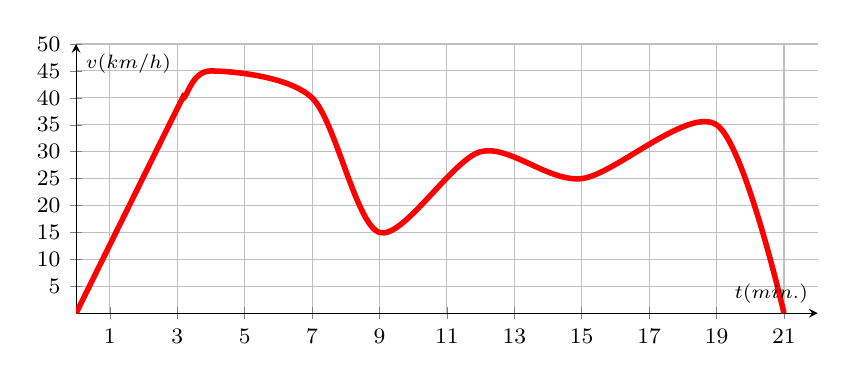
\begin{tikzpicture}[]
	\begin{axis}[width=11cm,height=5cm, axis background/.style={fill=white}, axis lines=middle, 
	grid = major,
	xlabel=$\scriptstyle t (min.)$,
	ylabel=$\scriptstyle v (km/h)$, 
	xtick={1,3,...,21},
	ytick={0,5,...,50},
	ymin = 0,
	ymax = 50,
	xmin = 0,
	xmax = 22,
	tick label style={font=\footnotesize},
	legend style={font=\normalsize,legend pos=south east},]
	\addplot[red, smooth, line width=2pt]  coordinates {(0,0) (3,38)   (3.2,40) (4, 45) (7, 40) (9,15) (12, 30)  (15, 25) (19, 35) (21, 0)};
	\end{axis}
	\end{tikzpicture}
\end{center}

\begin{tasks}
	\task Indica els intervals de creixement i decreixement.
	\task En què minuts va córrer a 10 km/h?
	\task Quina va ser la velocitat màxima i en quin minut passa? I mínima en ple trajecte?
	\task Quines altres característiques pots indicar sobre el gràfic?
\end{tasks}
\answers[cols=1]{[Creix a (0,\,4) i (9,\,12) i (15,\,19) min.; Decreix a (4,\,9) i (12,\,12) i (19,\,21) min., 1 min; 20.5 min, Màxim 45 km/h als 4 minuts i Mínima de 15 km/h als 9 min., És una funció contínua. El domini és (0,\,21) i el recorregut (0,\,45) ]}
	
\exer[2] Tenim una fotografia mida $10 \times 15$ que volem dibuixar sobre un quadre de mida $15P = 65 \times 50$. Justifica si serà possible encaixar tota la fotografia sense deformar-la. Si no és possible, explica quina part de la fotografia quedaria sense dibuixar.
\answers{No perquè $\dfrac{15}{10} \neq\dfrac{ 65}{60}$. Només podríem dibuixar 13 cm dels 15 cm de la fotografia.} 	
	
	
\exer[2]  En un triangle de costats 4 cm, 6 cm i 8 cm, calculau l'altura sobre el costat major. \textit{Ajuda:} Aplicau el teorema de Pitàgores i plantejau una equació.
\answers{$h=2,9$ cm}

\exer[2] Calcula l'àrea de la part pintada de les figures següents
\begin{tasks}(3)
	\task \includegraphics[width=0.2\textwidth, page=1]{img-12/arees}
	\task \includegraphics[width=0.2\textwidth, page=2]{img-12/arees}
	\task \includegraphics[width=0.2\textwidth, page=3]{img-12/arees}
\end{tasks}
\answers{$A=36$ cm$^2$, $A=32$ cm$^2$, $A=377$ cm$^2$}


\exer[2] Dibuixa en el teu quadern un triangle amb vèrtexs $A(1, 2)$, $B(2, 0)$ i $C(3, 4)$. Troba els vèrtexs de les figures segons les transformacions:
\begin{tasks}
	\task Una translació de vector $\vec t(3,-2)$
	\task Una simetria d'eix OX
	\task Una rotació de centre O(0,0) i angle 90$^\circ$.
	\task Una simetria que té per eix la recta que passa pels punts $P(3, 4)$ i $Q(7, 0)$.
\end{tasks}
\answers[cols=1]{[$A'(4,0)$ $B'(5,-2)$  $C'(6,2)$, $A'(1,-2)$ $B'(2,0)$ $C'(3,-4)$, $A'(-2,1)$ $B'(0,2)$ $C'(-4,3)$, $A'(5,6)$ $B'(7,5)$ $C'(3,4)$]}

\exer[2] La piràmide de Kheops és una piràmide de base quadrangular de 230 m d'aresta i 147 m d'altura. Calcula l'àrea total i el volum d'aquesta piràmide. Dóna les respostes en hm$^2$ i hm$^3$.
\answers{$A_T =13,88$ hm$^{2}$, $V=2,59$ hm$^3$}

\vspace{-1.5cm}
\exer[2]\begin{minipage}[t]{0.7\textwidth}
Troba l'àrea total d'un prisma de base hexagonal de costat 6 cm i d'altura 10 cm. Calcula també el volum del prisma.
\end{minipage}
\begin{minipage}{0.3\textwidth}
	\centering
	\vspace{1.5cm}
	\includegraphics[width=0.5\textwidth]{img-12/prisma-hexagonal}
\end{minipage}
\answers{$A_T =547,06$ cm$^{2}$, $V=935,3$ cm$^3$}	
 
 
\vspace*{-1.5cm}
\exer[2]\begin{minipage}[t]{0.7\textwidth}
	 Hem truncat un cub d'aresta 10 cm segons el pla ratllat de la figura. Calcula la superfície de la cara ratllada i el volum del cos.
\end{minipage}
\begin{minipage}{0.3\textwidth}
	\centering
	\vspace{1.5cm}
	\includegraphics[width=0.5\textwidth]{img-12/cubtruncat}
\end{minipage}
\answers{$A=50\sqrt{3}$ cm$^{2}$, $V=V_{cub} -V_{piram}=\frac{2500}{3}$ cm$^{3}$}	
	
	
	
\exer[2] Tenim 3 pilotes de tenis dins d'una caixa cilíndrica de 6,6 cm de diàmetre en la que encaixen perfectament. Calcula el volum de la part buida.
\begin{center}
	\includegraphics[width=0.35\textwidth]{img-12/tennis}
\end{center}	
\answers{$V=225.69$ cm$^3$}

\exer[2] Una piscina té forma d'ortoedre de dimensions $8\times 4 \times 2 $ m. Hem fet una lectura del pH de l'aigua de 6.8. Les recomanacions pel bany són que el pH estigui al voltant de 7.2. Per això, haurem afegir augmentador del pH del qual mostram l'etiqueta d'instruccions a la figura. Quina quantitat de producte haurem de posar per obtenir el pH desitjat?   
\begin{center}
	\includegraphics[width=0.75\textwidth]{img-12/phmas}
\end{center}	
\answers{Hem de posar 1.54 kg de pH+ per augmentar 0.4 punts.}


 \end{mylist}

	
 
	

\newpage 
\immediate\closeout\studentkeys
  
\def\currentname{Solucionari}
\fakechapter[\simbolclaubig]{ Solucions }
\addcontentsline{toc}{part}{Solucions}
\begin{multicols}{2}
	\fontsize{10.5}{12.6}\selectfont
	
 \vspace{1cm} 
 
 \needspace{5\baselineskip} 
 \heading{Solucions del Tema 1}

\vspace{0.3cm}

 \needspace{3\baselineskip} 

\hyperlink{page.9}{\textbf{\em Pàgina 9}}
\begin{enumerate}


 \needspace{2\baselineskip} 

\phantomsection
 \item[\fontfamily{phv}\selectfont\color{blue}\textbf{\ref{exer:5}. }] \label{ans:5}
 \begin{tasks}[column-sep=1em, item-indent=1.3333em](4)
	 \task $7$
	 \task $2$
	 \task $-3$
	 \task $-26$
\end{tasks}
 \end{enumerate}
\vspace{0.3cm}

 \needspace{3\baselineskip} 

\hyperlink{page.10}{\textbf{\em Pàgina 10}}
\begin{enumerate}


 \needspace{2\baselineskip} 

\phantomsection
 \item[\fontfamily{phv}\selectfont\color{blue}\textbf{\ref{exer:6}. }] \label{ans:6}
 \begin{tasks}[column-sep=1em, item-indent=1.3333em](4)
	 \task $\frac {3}{5}$
	 \task $\frac {1}{9}$
	 \task $\frac {1}{12}$
	 \task $\frac {1}{4}$
\end{tasks}
 \end{enumerate}
\begin{enumerate}


 \needspace{2\baselineskip} 

\phantomsection
 \item[\fontfamily{phv}\selectfont\color{blue}\textbf{\ref{exer:7}. }] \label{ans:7}
 \begin{tasks}[column-sep=1em, item-indent=1.3333em](4)
	 \task $1$
	 \task $\frac {11}{6}$
	 \task $\frac {17}{14}$
	 \task $\frac {7}{15}$
	 \task $\frac {31}{20}$
	 \task $-\frac {1}{8}$
	 \task $\frac {1}{4}$
	 \task $\frac {41}{24}$
\end{tasks}
 \end{enumerate}
\vspace{0.3cm}

 \needspace{3\baselineskip} 

\hyperlink{page.11}{\textbf{\em Pàgina 11}}
\begin{enumerate}


 \needspace{2\baselineskip} 

\phantomsection
 \item[\fontfamily{phv}\selectfont\color{blue}\textbf{\ref{exer:8}. }] \label{ans:8}
 \begin{tasks}[column-sep=1em, item-indent=1.3333em](3)
	 \task $\frac {2}{3}$
	 \task $8$
	 \task $\frac {1}{3}$
	 \task $\frac {1}{2}$
	 \task $\frac {1}{2}$
	 \task $1$
	 \task $\frac {5}{2}$
	 \task $2$
	 \task $-\frac {5}{6}$
	 \task $\frac {3}{2}$
	 \task $\frac {1}{3}$
	 \task $\frac {3}{5}$
\end{tasks}
 \end{enumerate}
\begin{enumerate}


 \needspace{2\baselineskip} 

\phantomsection
 \item[\fontfamily{phv}\selectfont\color{blue}\textbf{\ref{exer:13}. }] \label{ans:13}
 \begin{tasks}[column-sep=1em, item-indent=1.3333em](3)
	 \task $\frac {67}{4}$
	 \task $\frac {25}{4}$
	 \task $\frac {47}{8}$
\end{tasks}
 \end{enumerate}
\vspace{0.3cm}

 \needspace{3\baselineskip} 

\hyperlink{page.14}{\textbf{\em Pàgina 14}}
\begin{enumerate}


 \needspace{2\baselineskip} 

\phantomsection
 \item[\fontfamily{phv}\selectfont\color{blue}\textbf{\ref{exer:25}. }] \label{ans:25}
 \begin{tasks}[column-sep=1em, item-indent=1.3333em](3)
	 \task $1$
	 \task $\dfrac {20}{9}$
	 \task $\dfrac {99}{100}$
\end{tasks}
 \end{enumerate}
\vspace{0.3cm}

 \needspace{3\baselineskip} 

\hyperlink{page.19}{\textbf{\em Pàgina 19}}
\begin{enumerate}
\phantomsection
\item[\fontfamily{phv}\selectfont\color{blue}\textbf{\ref{exer:59}. }] \label{ans:59} 
10
 \end{enumerate}
\begin{enumerate}
\phantomsection
\item[\fontfamily{phv}\selectfont\color{blue}\textbf{\ref{exer:60}. }] \label{ans:60} 
$\frac {7}{8}>\frac {5}{6}>\frac {-5}{6}>\frac {-7}{8}>\frac {-5}{4}$
\phantomsection
\item[\fontfamily{phv}\selectfont\color{blue}\textbf{\ref{exer:62}. }] \label{ans:62} 
$\frac {7}{2}$


 \needspace{2\baselineskip} 

\phantomsection
 \item[\fontfamily{phv}\selectfont\color{blue}\textbf{\ref{exer:63}. }] \label{ans:63}
 \begin{tasks}[column-sep=1em, item-indent=1.3333em](2)
	 \task 180
	 \task 960 cm${}^3$
\end{tasks}


 \needspace{2\baselineskip} 

\phantomsection
 \item[\fontfamily{phv}\selectfont\color{blue}\textbf{\ref{exer:64}. }] \label{ans:64}
 \begin{tasks}[column-sep=1em, item-indent=1.3333em](1)
	 \task 9900,$E_A$=41,$E_R$=0.42\%
	 \task 9.9,$E_A$=0.045,$E_R$=0,45\% 
\end{tasks}


 \needspace{2\baselineskip} 

\phantomsection
 \item[\fontfamily{phv}\selectfont\color{blue}\textbf{\ref{exer:65}. }] \label{ans:65}
 \begin{tasks}[column-sep=1em, item-indent=1.3333em](2)
	 \task* Són exactes $\dfrac {6}{120}$ i $\dfrac {42}{150}$. $\dfrac {5}{180}$ és decimal periòdic
	 \task 10 xifres
	 \task 96 xifres
\end{tasks}
\phantomsection
\item[\fontfamily{phv}\selectfont\color{blue}\textbf{\ref{exer:66}. }] \label{ans:66} 
$\frac {89}{40}$, $\frac {2203}{990}$, $\frac {999}{1000}=0,999$


 \needspace{2\baselineskip} 

\phantomsection
 \item[\fontfamily{phv}\selectfont\color{blue}\textbf{\ref{exer:67}. }] \label{ans:67}
 \begin{tasks}[column-sep=1em, item-indent=1.3333em](2)
	 \task 4 setmanes
	 \task 506.25 cm${}^{3}$
\end{tasks}
\phantomsection
\item[\fontfamily{phv}\selectfont\color{blue}\textbf{\ref{exer:68}. }] \label{ans:68} 
Cobrava 1200 \euro {}. Ara cobra 1000 \euro {}, paga 250 \euro {} d'impostos i 300 \euro {} d'hipoteca. 
 \end{enumerate}

 \vspace{1cm} 
 
 \needspace{5\baselineskip} 
 \heading{Solucions del Tema 2}

\vspace{0.3cm}

 \needspace{3\baselineskip} 

\hyperlink{page.26}{\textbf{\em Pàgina 26}}
\begin{enumerate}


 \needspace{2\baselineskip} 

\phantomsection
 \item[\fontfamily{phv}\selectfont\color{blue}\textbf{\ref{exer:82}. }] \label{ans:82}
 \begin{tasks}[column-sep=1em, item-indent=1.3333em](2)
	 \task $2.231\cdot 10^6$
	 \task $5.678\cdot 10^{-3}$
	 \task $1.35\cdot 10^{-5}$
	 \task $3.6\cdot 10^{-4}$
\end{tasks}
 \end{enumerate}
\begin{enumerate}
\phantomsection
\item[\fontfamily{phv}\selectfont\color{blue}\textbf{\ref{exer:83}. }] \label{ans:83} 
$1.629\cdot 10^{17}$ m
\phantomsection
\item[\fontfamily{phv}\selectfont\color{blue}\textbf{\ref{exer:84}. }] \label{ans:84} 
La massa de l'isòtop C${}_{14}$ és: $6\times 1,672 \cdot 10^{-27} + 6 \times 9,11 \cdot 10^{-31}+ 8\times 1,64 \cdot 10^{-27} = 2.32\cdot 10^{-26}$ kg
 \end{enumerate}
\vspace{0.3cm}

 \needspace{3\baselineskip} 

\hyperlink{page.27}{\textbf{\em Pàgina 27}}
\begin{enumerate}
\phantomsection
\item[\fontfamily{phv}\selectfont\color{blue}\textbf{\ref{exer:86}. }] \label{ans:86} 
$50 t \cdot \frac {1\,000\,0000 \text { g}}{1 t} \cdot \frac {40\cdot 10^6 \text { bacteris}}{1 \text { g}}=4\cdot 10^{13}$ bacteris
 \end{enumerate}
\begin{enumerate}
\phantomsection
\item[\fontfamily{phv}\selectfont\color{blue}\textbf{\ref{exer:88}. }] \label{ans:88} 
$ 598 \cdot 10^{25} \text { g} \cdot \frac {50 \text { grans}}{1 \text { g}} \approx 3\cdot 10^{29}$ grans d'arena
 \end{enumerate}
\vspace{0.3cm}

 \needspace{3\baselineskip} 

\hyperlink{page.30}{\textbf{\em Pàgina 30}}
\begin{enumerate}


 \needspace{2\baselineskip} 

\phantomsection
 \item[\fontfamily{phv}\selectfont\color{blue}\textbf{\ref{exer:105}. }] \label{ans:105}
 \begin{tasks}[column-sep=1em, item-indent=1.3333em](2)
	 \task $a\cdot b\,\sqrt [4]{a^2 b}$
	 \task* $6^2 \cdot 3 \cdot 2^2 \sqrt [3]{3\cdot 6^2}$
	 \task $90\,\sqrt {45}$
\end{tasks}
 \end{enumerate}
\begin{enumerate}


 \needspace{2\baselineskip} 

\phantomsection
 \item[\fontfamily{phv}\selectfont\color{blue}\textbf{\ref{exer:106}. }] \label{ans:106}
 \begin{tasks}[column-sep=1em, item-indent=1.3333em](2)
	 \task $5^3\,\sqrt [{3}]{5}$
	 \task $3\sqrt {6}$
	 \task $\frac {2}{3}\sqrt {2}$
	 \task $\frac {x}{y^2}\sqrt {x }$
\end{tasks}
 \end{enumerate}
\vspace{0.3cm}

 \needspace{3\baselineskip} 

\hyperlink{page.32}{\textbf{\em Pàgina 32}}
\begin{enumerate}


 \needspace{2\baselineskip} 

\phantomsection
 \item[\fontfamily{phv}\selectfont\color{blue}\textbf{\ref{exer:118}. }] \label{ans:118}
 \begin{tasks}[column-sep=1em, item-indent=1.3333em](2)
	 \task $-\dfrac {1}{6}$
	 \task $144$
\end{tasks}
 \end{enumerate}
\begin{enumerate}


 \needspace{2\baselineskip} 

\phantomsection
 \item[\fontfamily{phv}\selectfont\color{blue}\textbf{\ref{exer:119}. }] \label{ans:119}
 \begin{tasks}[column-sep=1em, item-indent=1.3333em](2)
	 \task $30^4$
	 \task* $\left (-\dfrac {8}{5}\right )^7$
\end{tasks}


 \needspace{2\baselineskip} 

\phantomsection
 \item[\fontfamily{phv}\selectfont\color{blue}\textbf{\ref{exer:120}. }] \label{ans:120}
 \begin{tasks}[column-sep=1em, item-indent=1.3333em](3)
	 \task $(-2)^{15}$
	 \task $-1$
	 \task $(-5)^{4}$
\end{tasks}


 \needspace{2\baselineskip} 

\phantomsection
 \item[\fontfamily{phv}\selectfont\color{blue}\textbf{\ref{exer:121}. }] \label{ans:121}
 \begin{tasks}[column-sep=1em, item-indent=1.3333em](3)
	 \task $\dfrac {3}{5}$
	 \task $9$
	 \task $-\dfrac {125}{8}$
\end{tasks}
\phantomsection
\item[\fontfamily{phv}\selectfont\color{blue}\textbf{\ref{exer:122}. }] \label{ans:122} 
1


 \needspace{2\baselineskip} 

\phantomsection
 \item[\fontfamily{phv}\selectfont\color{blue}\textbf{\ref{exer:123}. }] \label{ans:123}
 \begin{tasks}[column-sep=1em, item-indent=1.3333em](2)
	 \task 310000000
	 \task $9.5 \cdot 10^{-9}$
\end{tasks}
\phantomsection
\item[\fontfamily{phv}\selectfont\color{blue}\textbf{\ref{exer:124}. }] \label{ans:124} 
140.75


 \needspace{2\baselineskip} 

\phantomsection
 \item[\fontfamily{phv}\selectfont\color{blue}\textbf{\ref{exer:125}. }] \label{ans:125}
 \begin{tasks}[column-sep=1em, item-indent=1.3333em](3)
	 \task $n=-125$
	 \task $n=2$
	 \task $n=-2$
\end{tasks}


 \needspace{2\baselineskip} 

\phantomsection
 \item[\fontfamily{phv}\selectfont\color{blue}\textbf{\ref{exer:126}. }] \label{ans:126}
 \begin{tasks}[column-sep=1em, item-indent=1.3333em](2)
	 \task* $\sqrt [{5}]{\left (-4\right )^{3}}$ Sí
	 \task $\sqrt {3}$ Sí
	 \task* $\sqrt [{4}]{\left (-5\right )^{3} }$ No
\end{tasks}


 \needspace{2\baselineskip} 

\phantomsection
 \item[\fontfamily{phv}\selectfont\color{blue}\textbf{\ref{exer:127}. }] \label{ans:127}
 \begin{tasks}[column-sep=1em, item-indent=1.3333em](2)
	 \task $5\sqrt [3]{5}$
	 \task $50\sqrt {10}$
\end{tasks}


 \needspace{2\baselineskip} 

\phantomsection
 \item[\fontfamily{phv}\selectfont\color{blue}\textbf{\ref{exer:128}. }] \label{ans:128}
 \begin{tasks}[column-sep=1em, item-indent=1.3333em](2)
	 \task $\frac {7}{3}\sqrt [3]{6}$
	 \task $\sqrt [30]{18}$
\end{tasks}
 \end{enumerate}

 \vspace{1cm} 
 
 \needspace{5\baselineskip} 
 \heading{Solucions del Tema 3}

\vspace{0.3cm}

 \needspace{3\baselineskip} 

\hyperlink{page.38}{\textbf{\em Pàgina 38}}
\begin{enumerate}
\phantomsection
\item[\fontfamily{phv}\selectfont\color{blue}\textbf{\ref{exer:149}. }] \label{ans:149} 
Sumen 355
 \end{enumerate}
\begin{enumerate}
\phantomsection
\item[\fontfamily{phv}\selectfont\color{blue}\textbf{\ref{exer:150}. }] \label{ans:150} 
Sumen 3825
\phantomsection
\item[\fontfamily{phv}\selectfont\color{blue}\textbf{\ref{exer:151}. }] \label{ans:151} 
98 \euro {}
 \end{enumerate}
\vspace{0.3cm}

 \needspace{3\baselineskip} 

\hyperlink{page.39}{\textbf{\em Pàgina 39}}
\begin{enumerate}
\phantomsection
\item[\fontfamily{phv}\selectfont\color{blue}\textbf{\ref{exer:157}. }] \label{ans:157} 
Raó $-2$, terme general $a_n=(-2)^n$
 \end{enumerate}
\begin{enumerate}
\phantomsection
\item[\fontfamily{phv}\selectfont\color{blue}\textbf{\ref{exer:160}. }] \label{ans:160} 
Els 15 primers termes sumen $\dfrac {163835}{16384}$
\phantomsection
\item[\fontfamily{phv}\selectfont\color{blue}\textbf{\ref{exer:161}. }] \label{ans:161} 
Els infinits termes sumen 12
 \end{enumerate}
\vspace{0.3cm}

 \needspace{3\baselineskip} 

\hyperlink{page.41}{\textbf{\em Pàgina 41}}
\begin{enumerate}


 \needspace{2\baselineskip} 

\phantomsection
 \item[\fontfamily{phv}\selectfont\color{blue}\textbf{\ref{exer:199}. }] \label{ans:199}
 \begin{tasks}[column-sep=1em, item-indent=1.3333em](2)
	 \task* $A_n = A \cdot (3/4)^{n-1}$ decreixent
	 \task* $P_n = 3L \cdot (3/2)^{n-1}$ creixent
\end{tasks}
 \end{enumerate}
\vspace{0.3cm}

 \needspace{3\baselineskip} 

\hyperlink{page.42}{\textbf{\em Pàgina 42}}
\begin{enumerate}
\phantomsection
\item[\fontfamily{phv}\selectfont\color{blue}\textbf{\ref{exer:201}. }] \label{ans:201} 
La raó és 3
 \end{enumerate}
\begin{enumerate}
\phantomsection
\item[\fontfamily{phv}\selectfont\color{blue}\textbf{\ref{exer:202}. }] \label{ans:202} 
Posició $n=335$
\phantomsection
\item[\fontfamily{phv}\selectfont\color{blue}\textbf{\ref{exer:203}. }] \label{ans:203} 
Sumen 340
\phantomsection
\item[\fontfamily{phv}\selectfont\color{blue}\textbf{\ref{exer:204}. }] \label{ans:204} 
És una progressió geomètrica. La raó és 3.
\phantomsection
\item[\fontfamily{phv}\selectfont\color{blue}\textbf{\ref{exer:205}. }] \label{ans:205} 
Progressió geomètrica $a_{n} = 2·5^{n-1}$ 
\phantomsection
\item[\fontfamily{phv}\selectfont\color{blue}\textbf{\ref{exer:206}. }] \label{ans:206} 
Sumem 2048
\phantomsection
\item[\fontfamily{phv}\selectfont\color{blue}\textbf{\ref{exer:207}. }] \label{ans:207} 
 $a_{ n} = 2n + 1$ 
\phantomsection
\item[\fontfamily{phv}\selectfont\color{blue}\textbf{\ref{exer:208}. }] \label{ans:208} 
250.000
\phantomsection
\item[\fontfamily{phv}\selectfont\color{blue}\textbf{\ref{exer:209}. }] \label{ans:209} 
192 pàgines dia 7; 381 pàgines en total
\phantomsection
\item[\fontfamily{phv}\selectfont\color{blue}\textbf{\ref{exer:210}. }] \label{ans:210} 
7299,92 \euro {}
 \end{enumerate}

 \vspace{1cm} 
 
 \needspace{5\baselineskip} 
 \heading{Solucions del Tema 4}

\vspace{0.3cm}

 \needspace{3\baselineskip} 

\hyperlink{page.48}{\textbf{\em Pàgina 48}}
\begin{enumerate}


 \needspace{2\baselineskip} 

\phantomsection
 \item[\fontfamily{phv}\selectfont\color{blue}\textbf{\ref{exer:219}. }] \label{ans:219}
 \begin{tasks}[column-sep=1em, item-indent=1.3333em](1)
	 \task* $\bar x=40.5$; $\sigma =16.5$; $CV=0.407$
	 \task* $\bar x=40.4$; $\sigma =17.11$; $CV=0.424$
	 \task* $\bar x=46.5$; $\sigma =9.74$; $CV=0.21$ \par \ggblink {https://goo.gl/JfqFSu}
\end{tasks}
 \end{enumerate}
\vspace{0.3cm}

 \needspace{3\baselineskip} 

\hyperlink{page.49}{\textbf{\em Pàgina 49}}
\begin{enumerate}
\phantomsection
\item[\fontfamily{phv}\selectfont\color{blue}\textbf{\ref{exer:220}. }] \label{ans:220} 
$M_o =1$; $\bar x=1.6$; $Var=0.84$; $\sigma =0.92$\par \ggblink {https://goo.gl/nKce19}
 \end{enumerate}
\begin{enumerate}
\phantomsection
\item[\fontfamily{phv}\selectfont\color{blue}\textbf{\ref{exer:221}. }] \label{ans:221} 
Variable quantitativa discreta;\par $\bar x=1.6078$; $\sigma =0.9717$\par \ggblink {https://goo.gl/9tu6n7}
\phantomsection
\item[\fontfamily{phv}\selectfont\color{blue}\textbf{\ref{exer:222}. }] \label{ans:222} 
$\bar x=0.95$; $M_o=1$; $M_e$ = 1; $Q_1 = 1$; $Q_3= 1$ \par \ggblink {https://goo.gl/nFytiW} 
 \end{enumerate}
\vspace{0.3cm}

 \needspace{3\baselineskip} 

\hyperlink{page.54}{\textbf{\em Pàgina 54}}
\begin{enumerate}


 \needspace{2\baselineskip} 

\phantomsection
 \item[\fontfamily{phv}\selectfont\color{blue}\textbf{\ref{exer:240}. }] \label{ans:240}
 \begin{tasks}[column-sep=1em, item-indent=1.3333em](3)
	 \task $\dfrac {58}{120}$
	 \task $\dfrac {16}{120}$
	 \task* $\dfrac {62}{120}$ i $\dfrac {1}{120}$ 
\end{tasks}
 \end{enumerate}
\vspace{0.3cm}

 \needspace{3\baselineskip} 

\hyperlink{page.55}{\textbf{\em Pàgina 55}}
\begin{enumerate}


 \needspace{2\baselineskip} 

\phantomsection
 \item[\fontfamily{phv}\selectfont\color{blue}\textbf{\ref{exer:245}. }] \label{ans:245}
 \begin{tasks}[column-sep=1em, item-indent=1.3333em](3)
	 \task $\frac {1}{2}$
	 \task $\frac {1}{2}$
	 \task $\frac {1}{2}$
	 \task* $1-\dfrac {1}{8}=\dfrac {7}{8}$
	 \task $\frac {1}{8}$
	 \task $\frac {1}{8}$
\end{tasks}
 \end{enumerate}
\begin{enumerate}


 \needspace{2\baselineskip} 

\phantomsection
 \item[\fontfamily{phv}\selectfont\color{blue}\textbf{\ref{exer:246}. }] \label{ans:246}
 \begin{tasks}[column-sep=1em, item-indent=1.3333em](3)
	 \task 0.19
	 \task 0.44
	 \task 0.56
	 \task 0.95
	 \task 0.65
	 \task 0.35
\end{tasks}
 \end{enumerate}
\vspace{0.3cm}

 \needspace{3\baselineskip} 

\hyperlink{page.56}{\textbf{\em Pàgina 56}}
\begin{enumerate}


 \needspace{2\baselineskip} 

\phantomsection
 \item[\fontfamily{phv}\selectfont\color{blue}\textbf{\ref{exer:248}. }] \label{ans:248}
 \begin{tasks}[column-sep=1em, item-indent=1.3333em](3)
	 \task $\dfrac {49}{100}$
	 \task $\dfrac {91}{100}$
	 \task $\dfrac {9}{100}$
\end{tasks}
 \end{enumerate}
\begin{enumerate}


 \needspace{2\baselineskip} 

\phantomsection
 \item[\fontfamily{phv}\selectfont\color{blue}\textbf{\ref{exer:249}. }] \label{ans:249}
 \begin{tasks}[column-sep=1em, item-indent=1.3333em](3)
	 \task $\dfrac {91}{100}$
	 \task $\dfrac {35}{38}$
	 \task $\dfrac {3}{38}$
\end{tasks}
 \end{enumerate}
\vspace{0.3cm}

 \needspace{3\baselineskip} 

\hyperlink{page.57}{\textbf{\em Pàgina 57}}
\begin{enumerate}
\phantomsection
\item[\fontfamily{phv}\selectfont\color{blue}\textbf{\ref{exer:252}. }] \label{ans:252} 
$P=0.9999$
 \end{enumerate}
\begin{enumerate}


 \needspace{2\baselineskip} 

\phantomsection
 \item[\fontfamily{phv}\selectfont\color{blue}\textbf{\ref{exer:256}. }] \label{ans:256}
 \begin{tasks}[column-sep=1em, item-indent=1.3333em](2)
	 \task $\dfrac {28}{153}$
	 \task $\dfrac {49}{153}$
	 \task $\dfrac {62}{153}$
	 \task $\dfrac {80}{153}$
\end{tasks}
 \end{enumerate}
\vspace{0.3cm}

 \needspace{3\baselineskip} 

\hyperlink{page.58}{\textbf{\em Pàgina 58}}
\begin{enumerate}
\phantomsection
\item[\fontfamily{phv}\selectfont\color{blue}\textbf{\ref{exer:259}. }] \label{ans:259} 
\textbf {--10.}: Claus de l'autoavaluació: 1b; 2c; 3c; 4b; 5d; 6a; 7a; 8b; 9d; 10c
 \end{enumerate}

 \vspace{1cm} 
 
 \needspace{5\baselineskip} 
 \heading{Solucions del Tema 5}

\vspace{0.3cm}

 \needspace{3\baselineskip} 

\hyperlink{page.66}{\textbf{\em Pàgina 66}}
\begin{enumerate}


 \needspace{2\baselineskip} 

\phantomsection
 \item[\fontfamily{phv}\selectfont\color{blue}\textbf{\ref{exer:292}. }] \label{ans:292}
 \begin{tasks}[column-sep=1em, item-indent=1.3333em](1)
	 \task $-3x^5+4x^4+2x^3$
	 \task $10x^4-8x^3+7x^2-3x$
	 \task $12\,a^3-43\,a^2+43\,a-10$
\end{tasks}
 \end{enumerate}
\vspace{0.3cm}

 \needspace{3\baselineskip} 

\hyperlink{page.67}{\textbf{\em Pàgina 67}}
\begin{enumerate}


 \needspace{2\baselineskip} 

\phantomsection
 \item[\fontfamily{phv}\selectfont\color{blue}\textbf{\ref{exer:293}. }] \label{ans:293}
 \begin{tasks}[column-sep=1em, item-indent=1.3333em](1)
	 \task $Q=3x-2$; $R=-2x+5$
	 \task $Q=-2$; $R=4x^2-x+6$
	 \task $Q=2x^2+3x$; $R=-16x+7$
	 \task $Q=3x^2-3x+4$; $R=-x+2$
	 \task $Q=x^3-3x$; $R=5x-6$
\end{tasks}
 \end{enumerate}
\begin{enumerate}


 \needspace{2\baselineskip} 

\phantomsection
 \item[\fontfamily{phv}\selectfont\color{blue}\textbf{\ref{exer:294}. }] \label{ans:294}
 \begin{tasks}[column-sep=1em, item-indent=1.3333em](1)
	 \task $Q=3x-11$; $R=38$
	 \task $Q=x^3+2x^2+4x+8$; $R=0$
	 \task $Q=x^3+x$; $R=1$
	 \task* $Q=7x^4-14x^3+24x^2-48x+103$; $R=-211$
\end{tasks}
 \end{enumerate}
\vspace{0.3cm}

 \needspace{3\baselineskip} 

\hyperlink{page.70}{\textbf{\em Pàgina 70}}
\begin{enumerate}


 \needspace{2\baselineskip} 

\phantomsection
 \item[\fontfamily{phv}\selectfont\color{blue}\textbf{\ref{exer:304}. }] \label{ans:304}
 \begin{tasks}[column-sep=1em, item-indent=1.3333em](3)
	 \task $\frac {3x+3}{x^2+x-2}$
	 \task $\frac {-4x+3}{x^2-x}$
	 \task $\frac {-3x^3+3x^2}{x^2+4x+3}$
	 \task $\frac {x^2-x-6}{x^3}$
\end{tasks}
 \end{enumerate}
\begin{enumerate}


 \needspace{2\baselineskip} 

\phantomsection
 \item[\fontfamily{phv}\selectfont\color{blue}\textbf{\ref{exer:305}. }] \label{ans:305}
 \begin{tasks}[column-sep=1em, item-indent=1.3333em](2)
	 \task $\frac {x^2+1}{x^3}$
	 \task $\frac {-x-1}{x^2-2x}$
\end{tasks}


 \needspace{2\baselineskip} 

\phantomsection
 \item[\fontfamily{phv}\selectfont\color{blue}\textbf{\ref{exer:309}. }] \label{ans:309}
 \begin{tasks}[column-sep=1em, item-indent=1.3333em](2)
	 \task $\frac {x-2}{3}$
	 \task $\frac {2(x-4)}{x+4}$
	 \task $\frac {-2}{2a+3}$
	 \task $\frac {x}{x-2}$
\end{tasks}
 \end{enumerate}
\vspace{0.3cm}

 \needspace{3\baselineskip} 

\hyperlink{page.73}{\textbf{\em Pàgina 73}}
\begin{enumerate}


 \needspace{2\baselineskip} 

\phantomsection
 \item[\fontfamily{phv}\selectfont\color{blue}\textbf{\ref{exer:326}. }] \label{ans:326}
 \begin{tasks}[column-sep=1em, item-indent=1.3333em](3)
	 \task $3x+5$
	 \task $(x+y)^2$
	 \task $\frac {2n}{3}$
\end{tasks}
 \end{enumerate}
\begin{enumerate}
\phantomsection
\item[\fontfamily{phv}\selectfont\color{blue}\textbf{\ref{exer:327}. }] \label{ans:327} 
$V=7\,x^2$
\phantomsection
\item[\fontfamily{phv}\selectfont\color{blue}\textbf{\ref{exer:328}. }] \label{ans:328} 
7


 \needspace{2\baselineskip} 

\phantomsection
 \item[\fontfamily{phv}\selectfont\color{blue}\textbf{\ref{exer:329}. }] \label{ans:329}
 \begin{tasks}[column-sep=1em, item-indent=1.3333em](3)
	 \task $15x^3$
	 \task $-\frac {5}{3}xy$
	 \task $2a^2 b$
\end{tasks}
\phantomsection
\item[\fontfamily{phv}\selectfont\color{blue}\textbf{\ref{exer:330}. }] \label{ans:330} 
Grau 4; terme independent 9; 4 termes


 \needspace{2\baselineskip} 

\phantomsection
 \item[\fontfamily{phv}\selectfont\color{blue}\textbf{\ref{exer:331}. }] \label{ans:331}
 \begin{tasks}[column-sep=1em, item-indent=1.3333em](1)
	 \task $Q=2x^2-5x+6$; $R=-2x-8$
	 \task $Q=3x^3+9x^2+22x+67$; $R=199$
\end{tasks}


 \needspace{2\baselineskip} 

\phantomsection
 \item[\fontfamily{phv}\selectfont\color{blue}\textbf{\ref{exer:332}. }] \label{ans:332}
 \begin{tasks}[column-sep=1em, item-indent=1.3333em](2)
	 \task* $\frac {4}{25}x^2 - \frac {4}{15}xy + \frac {y^2}{9}$
	 \task $x^4 - 1$
	 \task $9x^2+12x+4$
	 \task $2x^2 -5$
\end{tasks}


 \needspace{2\baselineskip} 

\phantomsection
 \item[\fontfamily{phv}\selectfont\color{blue}\textbf{\ref{exer:333}. }] \label{ans:333}
 \begin{tasks}[column-sep=1em, item-indent=1.3333em](1)
	 \task $5x^2 \cdot (1-3x+5x^2)$
	 \task* $x^2 y^2 \cdot (2 xy^3 - 3y^2 + 2 x^5 + 7xy)$
\end{tasks}


 \needspace{2\baselineskip} 

\phantomsection
 \item[\fontfamily{phv}\selectfont\color{blue}\textbf{\ref{exer:334}. }] \label{ans:334}
 \begin{tasks}[column-sep=1em, item-indent=1.3333em](2)
	 \task $x (x+1)^2$
	 \task $x^2 (x+1)(x-1)$
	 \task $3x^2 (x^2-8x+16)$
\end{tasks}
\phantomsection
\item[\fontfamily{phv}\selectfont\color{blue}\textbf{\ref{exer:335}. }] \label{ans:335} 
$\frac {2x}{x-1}$
\phantomsection
\item[\fontfamily{phv}\selectfont\color{blue}\textbf{\ref{exer:336}. }] \label{ans:336} 
$\frac {-x^2-5x+6}{2x^2}$
 \end{enumerate}

 \vspace{1cm} 
 
 \needspace{5\baselineskip} 
 \heading{Solucions del Tema 6}

\vspace{0.3cm}

 \needspace{3\baselineskip} 

\hyperlink{page.78}{\textbf{\em Pàgina 78}}
\begin{enumerate}


 \needspace{2\baselineskip} 

\phantomsection
 \item[\fontfamily{phv}\selectfont\color{blue}\textbf{\ref{exer:349}. }] \label{ans:349}
 \begin{tasks}[column-sep=1em, item-indent=1.3333em](4)
	 \task 3
	 \task 2
	 \task 2
	 \task 3
	 \task --1
	 \task 2/5
	 \task 1
	 \task 3/5
	 \task -1/2
	 \task -5
	 \task I.S.
	 \task S.S.
\end{tasks}
 \end{enumerate}
\begin{enumerate}


 \needspace{2\baselineskip} 

\phantomsection
 \item[\fontfamily{phv}\selectfont\color{blue}\textbf{\ref{exer:350}. }] \label{ans:350}
 \begin{tasks}[column-sep=1em, item-indent=1.3333em](4)
	 \task 2/3
	 \task 0
	 \task 2
	 \task 1/2
	 \task 3/4
	 \task --1
	 \task 8
	 \task 1/6
	 \task --2
	 \task 1
	 \task I.S.
	 \task S.S.
\end{tasks}


 \needspace{2\baselineskip} 

\phantomsection
 \item[\fontfamily{phv}\selectfont\color{blue}\textbf{\ref{exer:351}. }] \label{ans:351}
 \begin{tasks}[column-sep=1em, item-indent=1.3333em](4)
	 \task --1/3
	 \task --2
	 \task 2
	 \task 3
	 \task 5/7
	 \task 11
\end{tasks}
 \end{enumerate}
\vspace{0.3cm}

 \needspace{3\baselineskip} 

\hyperlink{page.79}{\textbf{\em Pàgina 79}}
\begin{enumerate}


 \needspace{2\baselineskip} 

\phantomsection
 \item[\fontfamily{phv}\selectfont\color{blue}\textbf{\ref{exer:352}. }] \label{ans:352}
 \begin{tasks}[column-sep=1em, item-indent=1.3333em](4)
	 \task 4/5
	 \task --1/3
	 \task --1/2
	 \task 5
	 \task 2
	 \task I.S.
	 \task S.S.
\end{tasks}
 \end{enumerate}
\vspace{0.3cm}

 \needspace{3\baselineskip} 

\hyperlink{page.80}{\textbf{\em Pàgina 80}}
\begin{enumerate}
\phantomsection
\item[\fontfamily{phv}\selectfont\color{blue}\textbf{\ref{exer:359}. }] \label{ans:359} 
En total 800 persones. Suspenen 424 en la primera prova i 94 en la segona.
 \end{enumerate}
\begin{enumerate}
\phantomsection
\item[\fontfamily{phv}\selectfont\color{blue}\textbf{\ref{exer:363}. }] \label{ans:363} 
cada disc 15 \euro {}; total 93 \euro {}
\phantomsection
\item[\fontfamily{phv}\selectfont\color{blue}\textbf{\ref{exer:365}. }] \label{ans:365} 
14 bé i 6 malament
\phantomsection
\item[\fontfamily{phv}\selectfont\color{blue}\textbf{\ref{exer:366}. }] \label{ans:366} 
12 monedes de 0.50 \euro {} i 8 monedes de 2 \euro {}
\phantomsection
\item[\fontfamily{phv}\selectfont\color{blue}\textbf{\ref{exer:367}. }] \label{ans:367} 
24 dromedaris i 62 camells
\phantomsection
\item[\fontfamily{phv}\selectfont\color{blue}\textbf{\ref{exer:368}. }] \label{ans:368} 
23 persones
 \end{enumerate}
\vspace{0.3cm}

 \needspace{3\baselineskip} 

\hyperlink{page.82}{\textbf{\em Pàgina 82}}
\begin{enumerate}


 \needspace{2\baselineskip} 

\phantomsection
 \item[\fontfamily{phv}\selectfont\color{blue}\textbf{\ref{exer:373}. }] \label{ans:373}
 \begin{tasks}[column-sep=1em, item-indent=1.3333em](2)
	 \task $x=0$ i $x=-2$
	 \task $x=\pm 3$
	 \task $x=\pm 5$
	 \task $x=0$ i $x=-1/2$
	 \task $x=-3/2$
	 \task $x=0$ i $x=2$
\end{tasks}
 \end{enumerate}
\vspace{0.3cm}

 \needspace{3\baselineskip} 

\hyperlink{page.84}{\textbf{\em Pàgina 84}}
\begin{enumerate}


 \needspace{2\baselineskip} 

\phantomsection
 \item[\fontfamily{phv}\selectfont\color{blue}\textbf{\ref{exer:383}. }] \label{ans:383}
 \begin{tasks}[column-sep=1em, item-indent=1.3333em](1)
	 \task $x=\pm 1$ i $x=\pm \sqrt {2}$
	 \task S.S.
	 \task $x=\pm \sqrt {6}$
\end{tasks}
 \end{enumerate}
\vspace{0.3cm}

 \needspace{3\baselineskip} 

\hyperlink{page.90}{\textbf{\em Pàgina 90}}
\begin{enumerate}
\phantomsection
\item[\fontfamily{phv}\selectfont\color{blue}\textbf{\ref{exer:427}. }] \label{ans:427} 
$x=2$ i $x=-6/5$
 \end{enumerate}
\begin{enumerate}
\phantomsection
\item[\fontfamily{phv}\selectfont\color{blue}\textbf{\ref{exer:428}. }] \label{ans:428} 
$x=13$ i $x=-12$
\phantomsection
\item[\fontfamily{phv}\selectfont\color{blue}\textbf{\ref{exer:429}. }] \label{ans:429} 
$x=5/3$ i $x=3$
\phantomsection
\item[\fontfamily{phv}\selectfont\color{blue}\textbf{\ref{exer:430}. }] \label{ans:430} 
$x=24$ i $x=8$
\phantomsection
\item[\fontfamily{phv}\selectfont\color{blue}\textbf{\ref{exer:431}. }] \label{ans:431} 
No té solució
\phantomsection
\item[\fontfamily{phv}\selectfont\color{blue}\textbf{\ref{exer:432}. }] \label{ans:432} 
Secants
\phantomsection
\item[\fontfamily{phv}\selectfont\color{blue}\textbf{\ref{exer:433}. }] \label{ans:433} 
No té solució
\phantomsection
\item[\fontfamily{phv}\selectfont\color{blue}\textbf{\ref{exer:434}. }] \label{ans:434} 
$x=2$ i $y=-1$
\phantomsection
\item[\fontfamily{phv}\selectfont\color{blue}\textbf{\ref{exer:435}. }] \label{ans:435} 
16 pollastres i 11 porcs
\phantomsection
\item[\fontfamily{phv}\selectfont\color{blue}\textbf{\ref{exer:436}. }] \label{ans:436} 
20 anys
 \end{enumerate}

 \vspace{1cm} 
 
 \needspace{5\baselineskip} 
 \heading{Solucions del Tema 7}

\vspace{0.3cm}

 \needspace{3\baselineskip} 

\hyperlink{page.100}{\textbf{\em Pàgina 100}}
\begin{enumerate}
\phantomsection
\item[\fontfamily{phv}\selectfont\color{blue}\textbf{\ref{exer:517}. }] \label{ans:517} 
160; 0.3; 90; 2000
 \end{enumerate}
\begin{enumerate}
\phantomsection
\item[\fontfamily{phv}\selectfont\color{blue}\textbf{\ref{exer:518}. }] \label{ans:518} 
1687.5 \euro {}
\phantomsection
\item[\fontfamily{phv}\selectfont\color{blue}\textbf{\ref{exer:519}. }] \label{ans:519} 
12.5 \%
\phantomsection
\item[\fontfamily{phv}\selectfont\color{blue}\textbf{\ref{exer:520}. }] \label{ans:520} 
480 botelles
\phantomsection
\item[\fontfamily{phv}\selectfont\color{blue}\textbf{\ref{exer:521}. }] \label{ans:521} 
16 t i 12.8 t
\phantomsection
\item[\fontfamily{phv}\selectfont\color{blue}\textbf{\ref{exer:522}. }] \label{ans:522} 
1:30\,000
\phantomsection
\item[\fontfamily{phv}\selectfont\color{blue}\textbf{\ref{exer:523}. }] \label{ans:523} 
5 rotllos
\phantomsection
\item[\fontfamily{phv}\selectfont\color{blue}\textbf{\ref{exer:524}. }] \label{ans:524} 
1,05\euro {}
\phantomsection
\item[\fontfamily{phv}\selectfont\color{blue}\textbf{\ref{exer:525}. }] \label{ans:525} 
64 camions
\phantomsection
\item[\fontfamily{phv}\selectfont\color{blue}\textbf{\ref{exer:526}. }] \label{ans:526} 
16329,35 \euro {}
 \end{enumerate}

 \vspace{1cm} 
 
 \needspace{5\baselineskip} 
 \heading{Solucions del Tema 8}

\vspace{0.3cm}

 \needspace{3\baselineskip} 

\hyperlink{page.111}{\textbf{\em Pàgina 111}}
\begin{enumerate}
\phantomsection
\item[\fontfamily{phv}\selectfont\color{blue}\textbf{\ref{exer:573}. }] \label{ans:573} 
\textbf {--6.} Autoavaluació: 1b; 2d; 3a; 4c; 5b; 6b
 \end{enumerate}

 \vspace{1cm} 
 
 \needspace{5\baselineskip} 
 \heading{Solucions del Tema 9}

\vspace{0.3cm}

 \needspace{3\baselineskip} 

\hyperlink{page.116}{\textbf{\em Pàgina 116}}
\begin{enumerate}


 \needspace{2\baselineskip} 

\phantomsection
 \item[\fontfamily{phv}\selectfont\color{blue}\textbf{\ref{exer:584}. }] \label{ans:584}
 \begin{tasks}[column-sep=1em, item-indent=1.3333em](1)
	 \task $x=4$ i $y=3$ cm
	 \task $x=6$ i $y=18$ cm
\end{tasks}
 \end{enumerate}
\vspace{0.3cm}

 \needspace{3\baselineskip} 

\hyperlink{page.117}{\textbf{\em Pàgina 117}}
\begin{enumerate}
\phantomsection
\item[\fontfamily{phv}\selectfont\color{blue}\textbf{\ref{exer:590}. }] \label{ans:590} 
$x=8$ cm
 \end{enumerate}
\vspace{0.3cm}

 \needspace{3\baselineskip} 

\hyperlink{page.118}{\textbf{\em Pàgina 118}}
\begin{enumerate}
\phantomsection
\item[\fontfamily{phv}\selectfont\color{blue}\textbf{\ref{exer:607}. }] \label{ans:607} 
$A=4.5$ cm$^2$, $P=15.62$ cm
 \end{enumerate}
\vspace{0.3cm}

 \needspace{3\baselineskip} 

\hyperlink{page.119}{\textbf{\em Pàgina 119}}
\begin{enumerate}
\phantomsection
\item[\fontfamily{phv}\selectfont\color{blue}\textbf{\ref{exer:621}. }] \label{ans:621} 
$A=10^2-\pi 5^2=21.46$ cm$^2$
 \end{enumerate}
\vspace{0.3cm}

 \needspace{3\baselineskip} 

\hyperlink{page.120}{\textbf{\em Pàgina 120}}
\begin{enumerate}
\phantomsection
\item[\fontfamily{phv}\selectfont\color{blue}\textbf{\ref{exer:626}. }] \label{ans:626} 
$A=\frac {9}{2}+ \frac {135}{360} \cdot \pi \cdot 18 = 25.71$ cm$^2$
 \end{enumerate}
\begin{enumerate}
\phantomsection
\item[\fontfamily{phv}\selectfont\color{blue}\textbf{\ref{exer:628}. }] \label{ans:628} 
$P=62.83$ cm i $A=222.03$ cm$^2$
 \end{enumerate}
\vspace{0.3cm}

 \needspace{3\baselineskip} 

\hyperlink{page.126}{\textbf{\em Pàgina 126}}
\begin{enumerate}
\phantomsection
\item[\fontfamily{phv}\selectfont\color{blue}\textbf{\ref{exer:692}. }] \label{ans:692} 
\textbf {--10.} Autoavaluació: 1d; 2b; 3c; 4a; 5d; 6a; 7a; 8c; 9d; 10a
 \end{enumerate}

 \vspace{1cm} 
 
 \needspace{5\baselineskip} 
 \heading{Solucions del Tema 10}

\vspace{0.3cm}

 \needspace{3\baselineskip} 

\hyperlink{page.130}{\textbf{\em Pàgina 130}}
\begin{enumerate}


 \needspace{2\baselineskip} 

\phantomsection
 \item[\fontfamily{phv}\selectfont\color{blue}\textbf{\ref{exer:716}. }] \label{ans:716}
 \begin{tasks}[column-sep=1em, item-indent=1.3333em](1)
	 \task $(-17,15)$
	 \task $(23,-7)$
	 \task $(-11,-14)$
\end{tasks}
 \end{enumerate}
\vspace{0.3cm}

 \needspace{3\baselineskip} 

\hyperlink{page.131}{\textbf{\em Pàgina 131}}
\begin{enumerate}
\phantomsection
\item[\fontfamily{phv}\selectfont\color{blue}\textbf{\ref{exer:721}. }] \label{ans:721} 
És una translació de vector $\vec t_1 + \vec t_2 = (-1,-1)$
 \end{enumerate}
\vspace{0.3cm}

 \needspace{3\baselineskip} 

\hyperlink{page.132}{\textbf{\em Pàgina 132}}
\begin{enumerate}
\phantomsection
\item[\fontfamily{phv}\selectfont\color{blue}\textbf{\ref{exer:727}. }] \label{ans:727} 
\textit {A'} (2, 4), \textit {B'} ($-$2, 3) i \textit {C'} (0, 5)
 \end{enumerate}
\begin{enumerate}
\phantomsection
\item[\fontfamily{phv}\selectfont\color{blue}\textbf{\ref{exer:730}. }] \label{ans:730} 
 Un gir de $60^\circ $ no deixa cap recta invariant. Un gir de $180^\circ $ deixa invariants les rectes que passen del centre de gir. Les rotacions de $0^\circ $ i $360^\circ $ són la identitat, deixen la figura original. 
 \end{enumerate}
\vspace{0.3cm}

 \needspace{3\baselineskip} 

\hyperlink{page.133}{\textbf{\em Pàgina 133}}
\begin{enumerate}
\phantomsection
\item[\fontfamily{phv}\selectfont\color{blue}\textbf{\ref{exer:738}. }] \label{ans:738} 
i) $A'(-3,-4)$, $B'(-5,6)$ i $C'(4,5)$;\par ii) $A'(3,4)$, $B'(5,-6)$ i $C'(-4,-5)$
 \end{enumerate}
\vspace{0.3cm}

 \needspace{3\baselineskip} 

\hyperlink{page.138}{\textbf{\em Pàgina 138}}
\begin{enumerate}
\phantomsection
\item[\fontfamily{phv}\selectfont\color{blue}\textbf{\ref{exer:768}. }] \label{ans:768} 
\textbf {--10. } Autoavaluació: 1b; 2c; 3b; 4d; 5c; 6b; 7b; 8b; 9d; 10b;
 \end{enumerate}

 \vspace{1cm} 
 
 \needspace{5\baselineskip} 
 \heading{Solucions del Tema 11}

\vspace{0.3cm}

 \needspace{3\baselineskip} 

\hyperlink{page.142}{\textbf{\em Pàgina 142}}
\begin{enumerate}
\phantomsection
\item[\fontfamily{phv}\selectfont\color{blue}\textbf{\ref{exer:787}. }] \label{ans:787} 
Teorema de Pitàgores a l'espai:\par $D=\sqrt {2^2+2^2+2^2}=3.46$ dm
 \end{enumerate}
\begin{enumerate}
\phantomsection
\item[\fontfamily{phv}\selectfont\color{blue}\textbf{\ref{exer:788}. }] \label{ans:788} 
Teorema de Pitàgores a l'espai:\par $D=\sqrt {10^2+4^2+3^2}=11.18$ m
\phantomsection
\item[\fontfamily{phv}\selectfont\color{blue}\textbf{\ref{exer:792}. }] \label{ans:792} 
$A_L=352$ cm$^2$
\phantomsection
\item[\fontfamily{phv}\selectfont\color{blue}\textbf{\ref{exer:793}. }] \label{ans:793} 
Totes les arestes mesuren $x=7.75$, l'altura d'una cara lateral $a_P=6.71$ i l'altura de la piràmide $H=5.48$ cm
 \end{enumerate}
\vspace{0.3cm}

 \needspace{3\baselineskip} 

\hyperlink{page.143}{\textbf{\em Pàgina 143}}
\begin{enumerate}
\phantomsection
\item[\fontfamily{phv}\selectfont\color{blue}\textbf{\ref{exer:796}. }] \label{ans:796} 
$A_L=4712.4$ dm$^2$
 \end{enumerate}
\begin{enumerate}


 \needspace{2\baselineskip} 

\phantomsection
 \item[\fontfamily{phv}\selectfont\color{blue}\textbf{\ref{exer:801}. }] \label{ans:801}
 \begin{tasks}[column-sep=1em, item-indent=1.3333em](2)
	 \task* $V=1000\pi =3140$ dm$^3$=litres
	 \task costarà 2400 \euro {}
\end{tasks}
 \end{enumerate}
\vspace{0.3cm}

 \needspace{3\baselineskip} 

\hyperlink{page.146}{\textbf{\em Pàgina 146}}
\begin{enumerate}
\phantomsection
\item[\fontfamily{phv}\selectfont\color{blue}\textbf{\ref{exer:839}. }] \label{ans:839} 
Apotema piràmide 4 m
 \end{enumerate}
\vspace{0.3cm}

 \needspace{3\baselineskip} 

\hyperlink{page.148}{\textbf{\em Pàgina 148}}
\begin{enumerate}


 \needspace{2\baselineskip} 

\phantomsection
 \item[\fontfamily{phv}\selectfont\color{blue}\textbf{\ref{exer:864}. }] \label{ans:864}
 \begin{tasks}[column-sep=1em, item-indent=1.3333em](1)
	 \task* $A=480$ cm$^2$ i $V=448$ cm$^3$
	 \task* $A=226.19$ cm$^2$ i $V=282.743$ cm$^3$
	 \task* $A=$depèn de l'inclinació i $V=125.66$ cm$^3$
	 \task* $A=277.24$ cm$^2$ i $V=368.61$ cm$^3$
\end{tasks}
 \end{enumerate}
\vspace{0.3cm}

 \needspace{3\baselineskip} 

\hyperlink{page.151}{\textbf{\em Pàgina 151}}
\begin{enumerate}
\phantomsection
\item[\fontfamily{phv}\selectfont\color{blue}\textbf{\ref{exer:888}. }] \label{ans:888} 
\textbf {--9.} Autoavaluació: 1c; 2a; 3d; 4b; 5a; 6d; 7b; 8a; 9c.
 \end{enumerate}

 \vspace{1cm} 
 
 \needspace{5\baselineskip} 
 \heading{Solucions del Tema 12}

\vspace{0.3cm}

 \needspace{3\baselineskip} 

\hyperlink{page.156}{\textbf{\em Pàgina 156}}
\begin{enumerate}
\phantomsection
\item[\fontfamily{phv}\selectfont\color{blue}\textbf{\ref{exer:898}. }] \label{ans:898} 
 a) $\frac {-5}{12}$;\quad b) $\frac {-3}{7}$
 \end{enumerate}
\begin{enumerate}
\phantomsection
\item[\fontfamily{phv}\selectfont\color{blue}\textbf{\ref{exer:899}. }] \label{ans:899} 
 $5^{20}$
\phantomsection
\item[\fontfamily{phv}\selectfont\color{blue}\textbf{\ref{exer:900}. }] \label{ans:900} 
a) 29 exercicis dia 15; \par b) 225 exercicis en total.
\phantomsection
\item[\fontfamily{phv}\selectfont\color{blue}\textbf{\ref{exer:901}. }] \label{ans:901} 
 a) $N=25$; $\sum f_i x_i = 41$; $\sum f_i x_i^2 =83$;\par c) $Mo=2$; $\bar x=1,64$; $\sigma =0,79$; $CV=0,48$ (48 \%).
\phantomsection
\item[\fontfamily{phv}\selectfont\color{blue}\textbf{\ref{exer:902}. }] \label{ans:902} 
 a) 0,51; b) 0,42
 \end{enumerate}
\vspace{0.3cm}

 \needspace{3\baselineskip} 

\hyperlink{page.157}{\textbf{\em Pàgina 157}}
\begin{enumerate}
\phantomsection
\item[\fontfamily{phv}\selectfont\color{blue}\textbf{\ref{exer:903}. }] \label{ans:903} 
 a) $3x^4+5x^3+2x^2-2x-4$; \par b) $3x^4+9x^3-8x^2+10x-5$; \par c) $-4x^4+4x^3+x^2-23x-3$; \par d) $4x^2+12x+9$
 \end{enumerate}
\begin{enumerate}
\phantomsection
\item[\fontfamily{phv}\selectfont\color{blue}\textbf{\ref{exer:904}. }] \label{ans:904} 
 a) $x=1,82$ i $x=-0,82$; \par b) $x=-1$ i $x=5$
\phantomsection
\item[\fontfamily{phv}\selectfont\color{blue}\textbf{\ref{exer:905}. }] \label{ans:905} 
 $x=-3$ i $y=7$
\phantomsection
\item[\fontfamily{phv}\selectfont\color{blue}\textbf{\ref{exer:906}. }] \label{ans:906} 
 Consumeixen $3000$ kWh
\phantomsection
\item[\fontfamily{phv}\selectfont\color{blue}\textbf{\ref{exer:907}. }] \label{ans:907} 
 $y=0.30 \cdot x + 100$; \quad $y=190$ €; \quad $x=65$ km
\phantomsection
\item[\fontfamily{phv}\selectfont\color{blue}\textbf{\ref{exer:908}. }] \label{ans:908} 
 Paràbola convexa en vèrtex al punt $x=5/2$, $y=17/4$
\phantomsection
\item[\fontfamily{phv}\selectfont\color{blue}\textbf{\ref{exer:909}. }] \label{ans:909} 
 $1.8585\cdots = \frac {184}{99}$ i $2.888 \cdots = \frac {26}{9}$. La mitjana és $x=\frac {235}{99}$. 
\phantomsection
\item[\fontfamily{phv}\selectfont\color{blue}\textbf{\ref{exer:910}. }] \label{ans:910} 
 947,37 \euro {} \ de sou brut
\phantomsection
\item[\fontfamily{phv}\selectfont\color{blue}\textbf{\ref{exer:911}. }] \label{ans:911} 
 a) $2,47\cdot 10^{-6}$ \quad b) $0,43943\cdots $ \quad c) 5 cm perquè $5^{3}$=125
\phantomsection
\item[\fontfamily{phv}\selectfont\color{blue}\textbf{\ref{exer:912}. }] \label{ans:912} 
 Per exemple, 17 anys = $5,36\cdot 10^{8}$ s
\phantomsection
\item[\fontfamily{phv}\selectfont\color{blue}\textbf{\ref{exer:913}. }] \label{ans:913} 
El dia 21 va nadar 115 minuts; durant els 21 dies va nadar 1365 minuts.
 \end{enumerate}
\vspace{0.3cm}

 \needspace{3\baselineskip} 

\hyperlink{page.158}{\textbf{\em Pàgina 158}}
\begin{enumerate}
\phantomsection
\item[\fontfamily{phv}\selectfont\color{blue}\textbf{\ref{exer:914}. }] \label{ans:914} 
 a) 38 hotels; c) mitjana=2.47; desv. típica=0.88; C.V. = 0.36 (36\%)
 \end{enumerate}
\begin{enumerate}
\phantomsection
\item[\fontfamily{phv}\selectfont\color{blue}\textbf{\ref{exer:915}. }] \label{ans:915} 
 a) grau 4; \quad b) $7x^{3}$; \quad c) 2 $x^{2}-4x$
\phantomsection
\item[\fontfamily{phv}\selectfont\color{blue}\textbf{\ref{exer:916}. }] \label{ans:916} 
 $P=6/11 \approx 0,54$
\phantomsection
\item[\fontfamily{phv}\selectfont\color{blue}\textbf{\ref{exer:917}. }] \label{ans:917} 
 $x=2y$; $x -8 = y+8$; \quad 3r A: $x= 32$; \quad 3r B: $y=16$.
\phantomsection
\item[\fontfamily{phv}\selectfont\color{blue}\textbf{\ref{exer:918}. }] \label{ans:918} 
 a) No té solució; \quad b) $x=-3$ i $x=3$; \par c) $x=0$ i $x=-2$; \quad d) $x=1$ i $x=-3$
\phantomsection
\item[\fontfamily{phv}\selectfont\color{blue}\textbf{\ref{exer:919}. }] \label{ans:919} 
 $x+30=\frac {x^2}{5}$; $x^2-5x-150=0$ $\rightarrow $ $x=-10$ no val; $x=15$ anys.
\phantomsection
\item[\fontfamily{phv}\selectfont\color{blue}\textbf{\ref{exer:920}. }] \label{ans:920} 
 Gastaran 672 \euro {} 
\phantomsection
\item[\fontfamily{phv}\selectfont\color{blue}\textbf{\ref{exer:921}. }] \label{ans:921} 
Ajuda: Utilitza l'equació de la funció lineal y= mx+n. Determina m i n. a) $y=-\frac {2}{3}x\ +\ 12$ ; \quad b) $\ 5=-\frac {2}{3}x\ +\ 12$ $\rightarrow $ $x=10,5$ hores
 \end{enumerate}
\vspace{0.3cm}

 \needspace{3\baselineskip} 

\hyperlink{page.159}{\textbf{\em Pàgina 159}}
\begin{enumerate}
\phantomsection
\item[\fontfamily{phv}\selectfont\color{blue}\textbf{\ref{exer:922}. }] \label{ans:922} 
 a) $y=3x+600$; \par b) $\mathrm {1230}\mathrm {\ }=3x+600$ $\rightarrow $ $x=210$ kg de taronges
 \end{enumerate}
\begin{enumerate}
\phantomsection
\item[\fontfamily{phv}\selectfont\color{blue}\textbf{\ref{exer:923}. }] \label{ans:923} 
 a) Lineal creixent; \quad b) paràbola còncava, $V(0,1)$; \quad Lineal decreixent


 \needspace{2\baselineskip} 

\phantomsection
 \item[\fontfamily{phv}\selectfont\color{blue}\textbf{\ref{exer:924}. }] \label{ans:924}
 \begin{tasks}[column-sep=1em, item-indent=1.3333em](1)
	 \task* Creix a (0,\,4) i (9,\,12) i (15,\,19) min.; Decreix a (4,\,9) i (12,\,12) i (19,\,21) min.
	 \task 1 min; 20.5 min
	 \task* Màxim 45 km/h als 4 minuts i Mínima de 15 km/h als 9 min.
	 \task* És una funció contínua. El domini és (0,\,21) i el recorregut (0,\,45) 
\end{tasks}
\phantomsection
\item[\fontfamily{phv}\selectfont\color{blue}\textbf{\ref{exer:925}. }] \label{ans:925} 
No perquè $\dfrac {15}{10} \neq \dfrac { 65}{60}$. Només podríem dibuixar 13 cm dels 15 cm de la fotografia.
\phantomsection
\item[\fontfamily{phv}\selectfont\color{blue}\textbf{\ref{exer:926}. }] \label{ans:926} 
$h=2,9$ cm
\phantomsection
\item[\fontfamily{phv}\selectfont\color{blue}\textbf{\ref{exer:927}. }] \label{ans:927} 
$A=36$ cm$^2$, $A=32$ cm$^2$, $A=377$ cm$^2$
 \end{enumerate}
\vspace{0.3cm}

 \needspace{3\baselineskip} 

\hyperlink{page.160}{\textbf{\em Pàgina 160}}
\begin{enumerate}


 \needspace{2\baselineskip} 

\phantomsection
 \item[\fontfamily{phv}\selectfont\color{blue}\textbf{\ref{exer:928}. }] \label{ans:928}
 \begin{tasks}[column-sep=1em, item-indent=1.3333em](1)
	 \task $A'(4,0)$ $B'(5,-2)$ $C'(6,2)$
	 \task* $A'(1,-2)$ $B'(2,0)$ $C'(3,-4)$
	 \task* $A'(-2,1)$ $B'(0,2)$ $C'(-4,3)$
	 \task $A'(5,6)$ $B'(7,5)$ $C'(3,4)$
\end{tasks}
 \end{enumerate}
\begin{enumerate}
\phantomsection
\item[\fontfamily{phv}\selectfont\color{blue}\textbf{\ref{exer:929}. }] \label{ans:929} 
$A_T =13,88$ hm$^{2}$, $V=2,59$ hm$^3$
\phantomsection
\item[\fontfamily{phv}\selectfont\color{blue}\textbf{\ref{exer:930}. }] \label{ans:930} 
$A_T =547,06$ cm$^{2}$, $V=935,3$ cm$^3$
\phantomsection
\item[\fontfamily{phv}\selectfont\color{blue}\textbf{\ref{exer:931}. }] \label{ans:931} 
$A=50\sqrt {3}$ cm$^{2}$, $V=V_{cub} -V_{piram}=250$ cm$^{3}$
\phantomsection
\item[\fontfamily{phv}\selectfont\color{blue}\textbf{\ref{exer:932}. }] \label{ans:932} 
$V=338,7$ cm$^3$
\phantomsection
\item[\fontfamily{phv}\selectfont\color{blue}\textbf{\ref{exer:933}. }] \label{ans:933} 
Hem de posar 1.54 kg de pH+ per augmentar 0.4 punts.
 \end{enumerate}
\end{multicols}

\end{document} 
